\documentclass[11pt]{article}
\usepackage[T1]{fontenc}
\usepackage{lmodern,amsmath,amssymb,amsthm,mathtools}
\usepackage[margin=1in]{geometry}
\setlength{\emergencystretch}{3em}
\usepackage{booktabs,longtable,array,enumitem,xcolor}
\usepackage[colorlinks=true,linkcolor=blue,urlcolor=blue]{hyperref}
% BEGIN ILLUSTRATION_20261026_C17_PACKAGES
\usepackage{tikz}
\usetikzlibrary{arrows.meta}
% END ILLUSTRATION_20261026_C17_PACKAGES
\newtheorem{theorem}{Theorem}[section]
\newtheorem{proposition}[theorem]{Proposition}
\newtheorem{lemma}[theorem]{Lemma}
\newtheorem{corollary}[theorem]{Corollary}
\theoremstyle{definition}
\newtheorem{definition}[theorem]{Definition}
\theoremstyle{remark}
\newtheorem{remark}[theorem]{Remark}
\newcommand{\R}{\mathbb R}
\newcommand{\HH}{\mathbb H}
\newcommand{\ip}[2]{\langle #1,#2\rangle}
\newcommand{\norm}[1]{\lVert #1\rVert}
\newcommand{\src}[1]{\textnormal{\textsf{[#1]}}}
\newcommand{\ph}{\varphi}
\title{Farthest vertices and a dimension bound for compact\\
hyperbolic Coxeter polytopes}
\author{CoxeterPolytopes project}
\date{25 October 2026}
\begin{document}
\maketitle
\begin{abstract}
We study a compact hyperbolic Coxeter polytope from one vertex farthest
from a fixed interior point. Its incident spherical diagram gives an
orthogonal decomposition of a single Euclidean vector of norm less than
one. Actual opposite walls, and points obtained from positive combinations
of actual walls, impose incompatible lower bounds on that vector.
The method has two branches: concave interpolation for \(A\)-chains,
and prefix interpolation followed by terminal-wall analysis for \(B\)-
and \(D\)-components. We prove that the dimension is at most \(17\).
Common geometric lemmas supply the component estimates; complete
actual-rank forest covers then reduce the proof to a small number
of whole-component configurations.
The last obstruction, a whole \(D_{18}\) diagram, is treated by a uniform
dotted-head pressure, legally funded reference vectors, the two genuine
signed fork directions, and a local calculation at an adjacent
\(A_{18}\) vertex. Arithmeticity is nowhere assumed.
\end{abstract}

\setcounter{tocdepth}{1}
\tableofcontents

\section{The theorem and the organization of its proof}
\label{sec:organization}
Our main result is the following dimension bound.
\begin{theorem}[Dimension bound]
\label{thm:main}
Every compact real hyperbolic Coxeter polytope has dimension at most \(17\).
\end{theorem}
Here compact means that every vertex is finite. The theorem concerns
arbitrary Coxeter reflection groups; there is no ground field, lattice,
integrality condition, or arithmetic hypothesis. It asserts an upper
bound, not sharpness or the existence of an example in dimension \(17\).

The central object is one vector \(x\), obtained from an original
farthest vertex \(p\). Energies of orthogonal components of its incident
diagram can be added because they are projections of this same vector.
Pressures arising from different auxiliary points cannot in general
be optimized separately and then added. Instead, we combine them in
one reference vector and retain its complete squared norm.

The case split occurs at the finite irreducible components of the
diagram at \(p\). Small components pay uniform energy debits.
A large \(A\)-component is handled in its zero-sum chain coordinates.
A large \(B\)- or \(D\)-component has a long common prefix; its terminal
nodes then require separate analysis. Section~\ref{sec:forests} records a
fresh complete cover at dimension \(18\), and the separate
higher-dimensional cover. A \emph{cover} always means necessary
possibilities, not realized examples. Section~\ref{sec:b18} explains the
whole-\(B_{18}\) terminal partition. Sections~\ref{sec:d18-setup}--%
\ref{sec:composition} give the whole-\(D_{18}\) closure.

The final composition has two parts. We exclude every dimension
at least \(19\) by its actual-rank forest cover and local consumers.
At dimension \(18\), the complete cover leaves only a whole
\(D_{18}\) diagram at the same selected farthest vertex. Neither boundary is obtained by taking a face
or deleting a node from a higher-dimensional list. We do not assume
that a face is Coxeter, or that the property under investigation is
inherited by faces.

\section{One original vector and actual geometric points}
\label{sec:geometry}
Use the hyperboloid model with Lorentz signature \((-+\cdots+)\).
Every wall has an outward unit spacelike normal \(n\), and the polytope
is given by \(\ip{r}{n}\leq0\). Distinct actual wall normals have
nonpositive products. Fix a strict interior point \(z\), choose an
actual vertex \(p\) farthest from \(z\), and write
\begin{equation}
\label{eq:original}
 z=E(p-x),\qquad E=-\ip{z}{p}>0,\qquad
 x\in p^\perp,\qquad \norm{x}^{2}=1-E^{-2}<1.
\end{equation}
The space \(p^\perp\) is Euclidean. The incident normals at \(p\) form
a positive definite spherical diagram; compact acute simplicity
implies that there are exactly \(n\) of them in dimension \(n\).
We retain these original normals and this original choice of
\(p,z,x,E\) throughout an energy argument.

The function \(r\mapsto-\ip{z}{r}\) takes its maximum on a compact
hyperbolic polytope at a vertex. Its restriction to a unit speed
geodesic has positive second derivative equal to the function itself,
so a maximum on a segment occurs at an endpoint; successively
passing to proper faces proves the assertion. Consequently
\begin{equation}
\label{eq:allpoint}
 -\ip{z}{r}\leq E\quad\text{for every actual point }r\in P.
\end{equation}
At an adjacent vertex \(q\), write \(z=E_q(q-y)\).
Equation~\eqref{eq:allpoint} gives a comparison factor \(E/E_q\),
not a claim that \(q\) is farthest.

\subsection{Positive inverse matrices and feasible projections}
\begin{lemma}[Inverse positivity]
\label{lem:inverse}
If a positive definite symmetric matrix \(B\) has nonpositive
off-diagonal entries, then \(B^{-1}\) is entrywise nonnegative.
\end{lemma}
\begin{proof}
Choose \(s\) greater than the largest eigenvalue of \(B\) and all its
diagonal entries. Then \(M=sI-B\) is entrywise nonnegative and has
spectral radius \(s-\lambda_{\min}(B)<s\). Thus
\(B^{-1}=s^{-1}\sum_{k\geq0}(M/s)^k\) is entrywise nonnegative.
\end{proof}
\begin{lemma}[An actual positive projection]
\label{lem:projection}
Let \(n_j\), \(j\in J\), be actual wall normals with positive
definite Gram matrix \(B_J\), and let \(z\) be strict interior.
Put
\[
 q_0=z-\sum_{i,j\in J}(B_J^{-1})_{ij}\ip{z}{n_j}n_i.
\]
Then \(q_0\) is future timelike, orthogonal to all selected walls,
and has negative product with every unselected actual wall.
Its normalization is a point of the original polytope.
\end{lemma}
\begin{proof}
The added coefficients are nonnegative by Lemma~\ref{lem:inverse}.
For an unselected wall every added product is nonpositive and the
original product is negative; the selected products vanish.
Moreover
\[
 q_0^2=z^2-
   (\ip{z}{n_i})_{i\in J}^{T}B_J^{-1}
   (\ip{z}{n_i})_{i\in J}<0.
\]
Since \(\ip{z}{q_0}=q_0^2<0\), it has future orientation.
All original wall inequalities survive normalization.
If fewer than \(n\) walls are selected this is a point on a face,
not an asserted full-dimensional vertex.
\end{proof}
The same sign check applies to positive combinations of actual
normals below: selected products are calculated explicitly; every
unknown original wall has nonpositive product with every summand.
A nonzero feasible future null vector would give a point of the
ideal boundary of \(P\), contradicting compactness. A positive
affine Coxeter kernel on actual walls is an obstruction after its
future sign and all remaining wall products have been checked.

\begin{lemma}[Future-point pressure]
\label{lem:pointpressure}
Suppose \(U\in p^\perp\), \(\xi=A p-U\) is future timelike
with \(\xi^2=-k<0\),
and its normalization is feasible against every actual wall.
Then the same original vector satisfies
\[
 \ip{x}{U}\geq A-\sqrt{k}.
\]
At a different actual vertex \(q\), use the decomposition
\(\xi=Aq-U\) with \(U\in q^\perp\). With all-point comparison
factor \(\kappa\), the corresponding inequality is
\(\ip{y}{U}\geq A-\kappa\sqrt{k}\).
\end{lemma}
\begin{proof}
The spatial hypothesis gives \(A=-\ip{p}{\xi}>0\).
Apply \eqref{eq:allpoint} to \(\xi/\sqrt{k}\):
\(-\ip{z}{\xi/\sqrt{k}}=E(A-\ip{x}{U})/\sqrt{k}\leq E\).
The modified comparison is the identical calculation.
\end{proof}
If \(U\ne0\), its support lies in actual orthogonal components
and \(\norm{U}^2=A^2-k\); Cauchy therefore also gives
\begin{equation}\label{eq:pointenergy}
 \norm{x_{\operatorname{supp}U}}^2
 \geq\frac{A-\sqrt{k}}{A+\sqrt{k}}.
\end{equation}
Normalize a future vector, not a spacelike correction.
For a cap \(c=A p-v\), clear a positive definite old block \(J\):
\[
 w=\sum_{i,j\in J}(B_J^{-1})_{ij}\beta_j n_i,\quad
 \beta_j=-\ip{c}{n_j}\geq0,\quad
 \eta=c+w,\quad \delta=\eta^2=1-\beta^TB_J^{-1}\beta.
\]
If \(\delta<0\), \(\eta\) is the future vector to normalize.
If \(\delta>0\), the actual finite projection instead uses
\[
 p+\frac{A}{\delta}\eta,\qquad
 \left(p+\frac{A}{\delta}\eta\right)^2=-1-\frac{A^2}{\delta}.
\]
When its selected products are nonpositive, its positive
coefficients check all unselected walls. The pressures are
\begin{equation}
\label{eq:corepressure}
 \ip{x}{v-w}\geq A-\sqrt{-\delta},\qquad
 \ip{x}{v-w}\geq
 \frac{A}{1+\sqrt{\delta/(A^2+\delta)}}.
\end{equation}
Old normals lie in \(p^\perp\), so \(v-w\) denotes the spatial
part of the corresponding displayed Lorentz vector.

\subsection{Opposite walls and common components}
Let \(B\) be the original incident Gram matrix, \(C=B^{-1}\), and
\[
 \omega_i=\sum_j C_{ij}n_j,\qquad
 d_i=C_{ii},\qquad u_i=\omega_i/\sqrt{d_i}.
\]
An actual opposite wall has normal
\[
 c=A p-v,\quad A>0,\quad
 v=\sum_i\beta_i\omega_i,\quad \beta_i=-\ip{c}{n_i}\geq0,\quad
 A^2=\beta^TC\beta-1.
\]
Strict interiority gives
\begin{equation}\label{eq:actualinterior}
 \ip{x}{v}<A.
\end{equation}
Along the original edge in direction \(-u_i\), of length \(L_i\),
the original farthest comparison gives
\begin{equation}
\label{eq:halfheight}
 \ip{x}{u_i}\geq\tanh(L_i/2).
\end{equation}
Whole-component projection energies sum to \(\norm{x}^2\).

\begin{proposition}[Reciprocal shadows; internal geometric interface]
\label{prop:shadows}
For an actual cap put \(T_i=(C\beta)_i/(A\sqrt{d_i})\).
If \(T_i>1\), it is the opposite wall of edge \(i\), and
\(\tanh L_i=1/T_i\). If it is not that opposite wall, then
\(\tanh L_i\geq T_i\). The value \(T_i=1\) is incompatible
with a finite endpoint. For distinct actual opposite walls,
\begin{equation}\label{eq:pair-shadow}
 \tanh L_i\,\tanh L_j\geq
 K_{ij},\qquad K_{ij}=C_{ij}/\sqrt{d_i d_j}.
\end{equation}
Opposite walls of orthogonal original directions cannot coincide.
\end{proposition}
\begin{proof}
The Schur identity says that
\(C-C_{\cdot i}C_{i\cdot}/d_i\) vanishes on row and column \(i\);
elsewhere it is the inverse of the retained old Gram matrix.
It is entrywise nonnegative. Let \(d=Dp-\sum_j\gamma_j\omega_j\)
be the actual opposite of edge \(i\), distinct from \(c\).
Acuteness and the Schur identity give
\[
 AD\geq\beta^TC\gamma
 \geq(C\beta)_i(C\gamma)_i/d_i.
\]
The actual endpoint equation is
\(\tanh L_i=D\sqrt{d_i}/(C\gamma)_i\), so
\(\tanh L_i\geq T_i\). If \(T_i>1\) this alternative is
impossible, forcing \(c=d\); its endpoint equation gives
\(\tanh L_i=1/T_i\).
If \(T_i=1\), the distinct alternative is impossible and the
same-wall equation would give an ideal endpoint. This is
excluded by compactness.
For the pair inequality, first use the contacts of the actual
opposite of \(i\) to get \(T_j\geq K_{ij}/\tanh L_i\);
the distinct alternative at edge \(j\) yields the assertion.

Finally suppose the same wall closes orthogonal directions
\(i,j\). Clearing every other old normal adds positive
coefficients and gives
\[
 c_F=A p-\frac{A}{r_i}u_i-\frac{A}{r_j}u_j,\qquad
 r_i=\tanh L_i,\quad r_j=\tanh L_j.
\]
Its product with the strict interior point remains negative,
so \(\ip{x}{u_i}/r_i+\ip{x}{u_j}/r_j<1\).
But \eqref{eq:halfheight} makes this sum at least
\(1+(\tau_i^2+\tau_j^2)/2>1\),
where \(\tau_i=\tanh(L_i/2)\). This contradiction proves
the orthogonal assertion.
\end{proof}
The displayed pair inequality concerns full tangents, not
half tangents.
For an opposite wall, its retained foreign component can have
at most one contact: two would make a cycle in its actual
finite replacement. A positive foreign cost is
\(q=\beta_j^2C_{jj}\geq1/4\). In a nontrivial component
\(C_{jj}\geq4/3\), so the only cost below \(1/3\) is a
simple \(3\)-contact on an \(A_1\), of cost \(1/4\).
Moreover
\begin{equation}\label{eq:foreigncost}
 q<A^2.
\end{equation}
Otherwise the actual reciprocal test would close that foreign
direction too, violating the orthogonal assertion, with the
equality case giving a null endpoint.
Set \(F(t)=2t/(1+t^2)\). For unit directions of correlation \(k\)
in a component of energy at most \(e\), positive heights satisfy
\begin{equation}\label{eq:pairupper}
 \tau_i+\tau_j\leq\sqrt{2e(1+k)},\qquad
 F(\tau_i)F(\tau_j)\leq\frac{4s}{(1+s)^2},\quad
 s=\frac{e(1+k)}2.
\end{equation}
The second inequality follows from concavity of \(\log F\) on
\((0,1)\). If its upper bound is smaller than \(K_{ij}\),
Proposition~\ref{prop:shadows} forces a common actual opposite.
Its finite-white extension or positive affine kernel then gives
additional actual pressures.

% BEGIN ILLUSTRATION_20261026_C17_BUDGET
\begin{figure}[tbp]
\centering
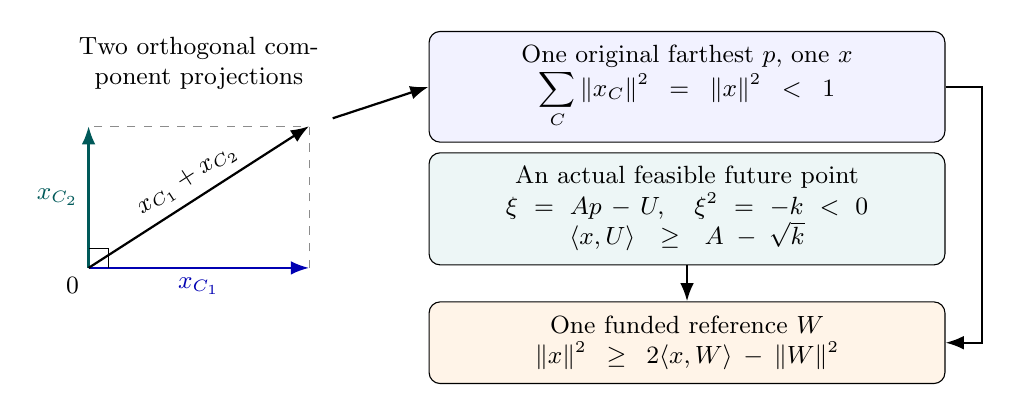
\begin{tikzpicture}[font=\small,>=Latex,
 box/.style={draw,rounded corners,align=center,text width=6.2cm,
 minimum height=.95cm,inner sep=5pt}]
 \coordinate (o) at (.4,.9);
 \coordinate (a) at (3.2,.9);
 \coordinate (b) at (.4,2.7);
 \coordinate (ab) at (3.2,2.7);
 \draw[->,thick,blue!70!black] (o)--(a)
   node[midway,below] {\(x_{C_1}\)};
 \draw[->,thick,teal!70!black] (o)--(b)
   node[midway,left] {\(x_{C_2}\)};
 \draw[->,thick] (o)--(ab)
   node[midway,above,sloped] {\(x_{C_1}+x_{C_2}\)};
 \draw[dashed,black!45] (a)--(ab)--(b);
 \draw (.65,.9)--(.65,1.15)--(.4,1.15);
 \node[below left] at (o) {\(0\)};
 \node[align=center,text width=4.1cm] at (1.8,3.5)
   {Two orthogonal component projections};
 \node[box,fill=blue!5] (budget) at (8.0,3.2)
   {One original farthest \(p\), one \(x\)\\
    \(\displaystyle\sum_C\|x_C\|^2=\|x\|^2<1\)};
 \node[box,fill=teal!7] (point) at (8.0,1.65)
   {An actual feasible future point\\
    \(\xi=Ap-U,\quad \xi^2=-k<0\)\\
    \(\langle x,U\rangle\ge A-\sqrt{k}\)};
 \node[box,fill=orange!9] (reference) at (8.0,-.05)
   {One funded reference \(W\)\\
    \(\|x\|^2\ge2\langle x,W\rangle-\|W\|^2\)};
 \draw[->,thick] (3.5,2.8)--(budget.west);
 \draw[->,thick] (point)--(reference);
 \draw[->,thick] (budget.east)--(11.75,3.2)
   --(11.75,-.05)--(reference.east);
\end{tikzpicture}
\caption{The single-vector budget and the actual-point pressure of
Lemma~\ref{lem:pointpressure}. The left panel is an abstract orthogonal
decomposition in \(p^\perp\), not a polytope realization. Whole-component
energies add; overlapping pressures are combined in one reference with
every individual coefficient debit and every cross term retained.}
\label{fig:ill20261026:c17:budget}
\end{figure}
% END ILLUSTRATION_20261026_C17_BUDGET
\section{Reference vectors, individual prices, and missing floors}
\label{sec:references}
The elementary estimate behind every certificate is
\begin{equation}
\label{eq:square}
 \norm{x}^2\geq2\ip{x}{W}-\norm{W}^2.
\end{equation}
Every term in \(\ip{x}{W}\) must be justified.
Write \(w=\sum_i b_iP_i\), \(b_i\geq0\), with actual pressures
\(\ip{x}{P_i}>a_i\), and demand \(A_w=\sum_i b_i a_i\).
For a new actual pressure \(\ip{x}{Z}\geq h\), choose
\[
 Q=Z-\sum_i t_iP_i,\qquad W=w+\mu Q.
\]
Before using pressures require \(\mu\geq0\) and check every
\(b_i-\mu t_i\geq0\).
Then
\begin{equation}
\label{eq:payment}
 \ip{x}{W}\geq A_w+\mu(h-\sum_i t_i a_i),\quad
 \norm{W}^2=\norm{w}^2+2\mu\ip{w}{Q}+\mu^2\norm{Q}^2.
\end{equation}
The available price \(b_i\) is individual to anchor \(i\).
The first inequality is strict if some strictly constrained old
anchor retains a positive coefficient, or if \(\mu>0\) and the
new pressure is strict. For multiple corrections every new weight
must be nonnegative; their combined debit at each anchor and all
mutual cross terms must be retained.

Put \(P_i=e_1+\cdots+e_i\), \(S_i=\ip{x}{P_i}\).
If selected indices satisfy \(S_i>f_i\), concave interpolation
through \((0,0)\) and the selected \((i,f_i)\) gives a reference
whose coordinates are successive slopes. Its \(P_i\) coefficients
are successive slope decreases, hence nonnegative; its demand
is its squared norm. Omitting one unknown internal floor replaces
two adjacent slopes by their average, losing half their squared
difference. For \(\sqrt t\) at \(t\geq5\), the loss is less than
\(1/3200\). Nonadjacent omissions have disjoint open intervals,
so losses add. A missing floor has coefficient zero.
References are Euclidean vectors, not asserted actual points:
actual points prove pressures, then positive coefficients combine
them in \eqref{eq:square}.

\section{Common component bounds and the precise branch point}
\label{sec:components}
\subsection{Ordinary components and exceptional actual defects}
All bounds below concern the same original projection, with
arbitrary finite spectators.
\begin{center}\small
\begin{tabular}{ll@{\qquad}ll}
\toprule
Component&Energy greater than&Component&Energy greater than\\ \midrule
ordinary nonshort \(A_1\)&\(1/10\)&ordinary \(A_2\)&\(319/2000\)\\
ordinary \(I_2(m),m\geq4\)&\(1/7\)&\(A_3\)&\(1/4\)\\
\(B_3,H_3\)&\(2/7\)&\(A_4\)&\(2/7\)\\
\(B_4,D_4,F_4\)&\(1/3\)&\(H_4\)&\(11/36\)\\
\(A_5\)&\(3/8\)&\(A_6\)&\(3/7\)\\
\(B_5,B_6\)&\(3/7\)&\(D_5,D_6\)&\(5/14,\ 3/7\)\\
\(B_7,D_7\)&\(1/2\)&\(B_8,D_8\)&\(4/7\)\\
\(E_6,E_7,E_8\)&\(9/20,\ 5/9,\ 2/3\)&&\\ \bottomrule
\end{tabular}
\end{center}
An actual isolated dotted short \(A_1\) is denoted \(I\).
A second short-wall profile \(J\) uses two old \(A_1\) factors
whose joint energy exceeds \(.34\).
The two typed rank-two exceptions, each of energy \(>.09\), are
\[
 N_7=(\text{old }A_2,\ \text{new isolated native }7),\qquad
 O_7=(\text{old }I_2(7),\ \text{new isolated native }3).
\]
A bare \(I_2(7)\) is not automatically \(O_7\).
There is at most one short \(I/J\) profile or one typed exception;
they do not coexist. Acuteness of their actual isolated walls
is essential: two on orthogonal supports would have product
\(-\sqrt{h_1h_2}\) strictly between \(-1/2\) and \(0\).
Appendix~\ref{app:ordinary} proves the endpoint estimates,
the \(J\) case and the ordinary rates.

Useful joint bounds, counting \(I\) only once, are
\begin{equation}
\label{eq:joint}
 I+A_1>1/5,\quad I+2A_1>3/10,\quad
 I+T_2>21/100,\quad I+T_3>2/7.
\end{equation}
Here \(T_j\) is ordinary irreducible of rank \(j\).
Both typed exceptions force another \(T_2\) to cost \(>1/5\).
Another \(A_1\) costs \(>1/5\) beside \(N_7\) and \(>2/15\)
beside \(O_7\). For the latter, isolated height
\(h=\tfrac14\csc^2(\pi/7)-1<1/3\) gives squared full tangent
greater than \(3/7\). Squared half tangent exceeds \(2/15\),
since \(4(2/15)/(1+2/15)^2=120/289<3/7\).
This is a real geometric argument.
The complete contact and defect proofs, including the actual-wall
height constraints behind \eqref{eq:joint}, are given in
Appendix~\ref{app:ordinary}. The uniform actual \(B/D\) floor
is proved in Appendix~\ref{app:BDfloor}.

\subsection[The A-chain branch]{The \(A\)-chain branch}
For \(A_r\), use the zero-sum subspace of \(\R^{r+1}\) with roots
\((e_i-e_{i+1})/\sqrt2\). The inverse Gram matrix is
\[
 C_{ij}=\frac{2\min(i,j)(r+1-\max(i,j))}{r+1}.
\]
A finite-white classification of actual opposite walls gives
strong dual floors except for a short list of literal helper caps.
Adjacent weak helpers are excluded using their actual mutual
product and a positive two-cap projection. Concave interpolation
uses only strong floors; helper pressures are paid at surviving
anchors. The small end variance yields stronger component bounds:
\[
\begin{array}{c|ccccc}
r&r\geq7&r\geq8&r\geq13&16&17\\ \hline
e(A_r)>&1/2&4/7&5/7&199/250&6/7
\end{array}
\qquad e(A_{18})>91/100.
\]
Later local refinements give \(e(A_{12})>13/20\) and
\(e(A_{15})>413/500\), uniformly with arbitrary spectators.
The shared actual feet, common-pair inventories, uniform
\(1/2,4/7,5/7\) bounds, and the \(N=17,18,19\) central-window
and paid-reference arguments are proved in Appendix~\ref{app:Achain}.
The newer \(A_{16}>.86\) proof in particular implies the older
\(.796\) bound without requiring its separate historical reference.
The fresh smaller-rank proofs are in Sections~\ref{app:A12}
and~\ref{app:A15}. Their full native-cosine inventories and
individual actual-helper payments are included. Later exact-\(17\)
research remains excluded.

\subsection[The common B/D prefix branch]{The common \(B/D\) prefix branch}
For \(B_r\), use long roots \((e_i-e_{i+1})/\sqrt2\), \(i<r\),
and short root \(e_r\). For \(D_r\), use the long chain and the
fork root \((e_{r-1}+e_r)/\sqrt2\). On a long initial segment,
\(\omega_i=\sqrt2P_i\), \(C_{ij}=2\min(i,j)\).
In type \(D\), \(x_1>\cdots>x_{r-1}>|x_r|\); the last
coordinate is signed and the forks are distinct actual duals.
\begin{proposition}[Generic prefix theorem]
\label{prop:prefix}
Let \(6\leq M\leq16\). Suppose an actual component is \(B_r\),
\(r\geq M+5\), or \(D_r\), \(r\geq M+6\). Put
\[
 f_i=\sqrt i-\frac{61}{100\sqrt2},\quad
 E_M=\frac{f_5^2}{5}+\sum_{i=5}^{M-1}(\sqrt{i+1}-\sqrt i)^2,
 \quad H_M=\left\lfloor\frac{M-5}{2}\right\rfloor.
\]
With arbitrary finite spectators,
\(\sum_{j=1}^{M+1}x_j^2>E_M-H_M/3200\).
\end{proposition}
\begin{proof}
Appendix~\ref{app:prefixinventory} proves that a weak site
\(5\leq i\leq M+1\) has a pure cap
\[
 v=\gamma\omega_i+\omega_1/2,\quad
 A^2=2i\gamma^2+2\gamma-\tfrac12,\quad
 101/125<\gamma<6/5,
\]
with own label \(5\), finite label at least \(7\), or dotted own
contact, and no spectator contact. Actual weak sites are
nonadjacent. This is proved at these ranks, not transferred from
a whole-component exclusion.
If \(5\) is strong, choose a strong \(K=M\) or \(M+1\).
Interpolate through actual strong knots. Each missing internal
floor loses \(<1/3200\); at \(K=M+1\) the extra increment
\((\sqrt{M+1}-\sqrt M)^2>1/(4M+2)\geq1/66\)
pays the possible extra omission.

If \(5\) is weak, the first-six-root point table in
Appendix~\ref{app:prefixinventory} gives \(x_1>.5965\), and \(6\) is strong, with
\(S_6>2.01815\). Interpolate through \((1,.5965),(6,2.01815)\)
and a later strong endpoint. The slopes decrease:
\(.5965,.28433\), then \(1/(\sqrt K+\sqrt6)<1/5\).
Its energy exceeds
\[
 L_M=.7600299945+\frac{(\sqrt M-\sqrt6)^2}{M-6},
\]
the last term being zero at \(M=6\).
Now \(E_6<.7\). The \(k=M-6\) increments from \(6\) onward lie
in \((1/8,1/5)\), so their variance is at most
\(k(1/5-1/8)^2/4\leq9/640\).
Thus \(L_M-E_M>.76-.7-9/640>0\), directly also at \(M=6\).
This proves the weak-\(5\) branch without first assuming strong \(5\).
\end{proof}
Appendix~\ref{app:prefixinventory} supplies the complete
finite-white inventory, zero-own repair, actual two-cap
nonadjacency, all four weak-\(5\) pressures and continuous
seals, with every spectator retained. Its original rank
inequalities are part of the theorem. A short-tail continuation
at an excluded rank still requires its own new local proof.

\section{Complete forest covers and their consumers}
\label{sec:forests}
\subsection[A fresh cover in exact dimension 18]{A fresh cover in exact dimension \(18\)}
Call \(A_r\), \(r\geq7\), or \(B_r,D_r\), \(r\geq9\),
dominant. Each costs \(>1/2\), so at most one is possible.
With none the ordinary rank-over-\(14\) baseline, even allowing
the unique defect, exceeds \(1\). Exactly one is therefore present.
The fresh total-rank-\(18\) necessary cover is:
\begin{center}\small
\begin{tabular}{p{.14\linewidth}p{.75\linewidth}}
\toprule
Dominant&All retained spectator alternatives\\ \midrule
\(A_{12}\)&\(I+(A_5\text{ or }D_5)\), or \(N_7/O_7+T_4\)\\
\(A_{15}\)&ordinary \(A_3\); \(T_2+A_1\); \(I+T_2\); or \(O_7+A_1\)\\
\(A_{16}\)&ordinary \(T_2\); two ordinary \(A_1\); \(I+A_1\); or \(N_7/O_7\)\\
\(A_{17}\)&one ordinary nonshort \(A_1\), or \(I\)\\
\(A_{18}\)&none\\
\(B_{16}\)&\(N_7/O_7\)\\
\(B_{17}\)&\(I\)\\
\(B_{18}\)&none\\
\(D_{16}\)&\(N_7/O_7\)\\
\(D_{17}\)&one ordinary nonshort \(A_1\), or \(I\)\\
\(D_{18}\)&none\\ \bottomrule
\end{tabular}
\end{center}
Here ordinary \(T_2=I_2(m)\), \(m\geq3\), and
\(T_4\in\{A_4,B_4,D_4,F_4,H_4\}\).
\(H_4\) and native \(5\) are not discarded by field arguments.

For completeness, the accounting steps are as follows.
\(A_7\) leaves too many ordinary ranks;
\(A_8,\ldots,A_{11}\) are excluded by \(4/7\) plus
the rank-over-\(14\) baseline.
Beside \(A_{12}\), ordinary or \(J\) rank-six spectators cost
\(>3/7\). With \(I\), \eqref{eq:joint} excludes all rank-five
partitions except \(A_5,D_5\). With a typed exception, partition
rank \(4\): two \(T_2\)'s cost \(>.4\), \(T_3+A_1\) costs
\(>1/4+2/15\), and the other reducible partitions are stronger.
Only irreducible \(T_4\) remains. For \(A_{13},A_{14}\),
the \(5/7\) bound and \eqref{eq:joint} exclude all spectators.
At \(A_{15}\), exclude \(B_3,H_3\), three ordinary \(A_1\)'s,
\(I+2A_1\), \(J+A_1\), and \(N_7+A_1\).
At \(A_{16}\), \(.796\) excludes \(J\) but retains precisely
the listed rank-two alternatives. At \(A_{17}\) retain the
remaining \(A_1\).

For \(B_r,D_r\), the \(9/14\) bound forces spectator rank
at most \(5\), hence \(r\geq13\).
Proposition~\ref{prop:prefix}, within its rank domain, gives
\[
\begin{array}{c|rrrr}
r&13&14&15&16\\ \hline
e(B_r),e(D_r)>&.7349975&.7683275&.797425&.823735.
\end{array}
\]
At \(13,14,15\), every ordinary, \(I/J\), and typed remainder
exceeds the residual budget; \(I+T_2>.21\) closes rank \(15\).
At \(16\), two ordinary \(A_1\)'s and \(I+A_1\) are excluded;
ordinary \(T_2\) and both typed defects initially remain.
The \(B_3,D_4,D_3\) layer checks in
Appendix~\ref{app:exact18layers} extend helper coverage to \(13\), giving
energy \(>.8689525\); ordinary \(T_2>1/7\) closes that case.
The fresh \(B_{17}\) layers reach a strong \(14/15\) endpoint
and energy \(>.90715\), excluding a nonshort ordinary \(A_1\).
This reuses the interpolation proof after new local coverage,
not Proposition~\ref{prop:prefix} outside its legal ranks.

The first rows close with small shared consumers:
\[
 A_{12}+I+(A_5/D_5)>13/20+5/14=141/140,\quad
 A_{12}+N_7/O_7+T_4>13/20+.09+2/7=359/350.
\]
The improved \(413/500\) bound closes every \(A_{15}\) family:
ordinary total rank three costs \(>17/70\), \(I+T_2>.21\),
and beside \(O_7+A_1\) the total exceeds \(787/750\).
Thus the older separate ordinary-rank-three consumer is unnecessary.
The other internal proof homes are:
\begin{center}\small
\begin{tabular}{lp{.69\linewidth}}
\toprule
Row&Excluding project argument\\ \midrule
\(A_{16}\)&Proposition~\ref{app:prop:A16}, ordinary and \(I+A_1\);
 Appendix~\ref{app:A16typed18}, both actual typed defects\\
\(A_{17}\)&Appendix~\ref{app:A17rankone18}, ordinary and actual \(I\)\\
whole \(A_{18}\)&Appendix~\ref{app:wholeA18}, full two-end native-gap argument\\
\(B_{16}\)&Appendix~\ref{app:BD16typed18}, both actual typed defects\\
\(B_{17}\)&Appendix~\ref{app:B17I18}, actual \(I\); local head and helper kernels\\
\(D_{16}\)&Appendix~\ref{app:BD16typed18}, both actual typed defects\\
\(D_{17}\)&Appendices~\ref{app:D17ordinary18} and~\ref{app:D17I18},
 ordinary and actual \(I\)\\
whole \(B_{18}\)&Section~\ref{sec:b18}\\
whole \(D_{18}\)&Sections~\ref{sec:d18-setup}--\ref{sec:composition}\\
\bottomrule
\end{tabular}
\end{center}
Appendix~\ref{app:exact18layers} proves the local layers used in
this cover, including the distinct signed \(D_4/D_3\) forks and the
actual \(A_{17}\) neighbor for \(B_{17}\). The table identifies the
complete proof of every retained row, including both short rank-one
cases. The independent higher-dimensional exclusions are proved in
Appendices~\ref{app:highertail}--\ref{app:exact19:wholeD19proof}.
These arguments use no field, lattice or integral dotted-product
hypothesis.

\subsection{The separate complete higher-dimensional tail}
\label{subsec:higher}
The exact-\(18\) cover does not exclude higher dimensions.
The earlier internal package establishes the separate theorem:
\begin{theorem}[Internal higher-dimensional exclusion]
\label{thm:tail}
There is no compact hyperbolic Coxeter polytope of dimension at least \(19\).
\end{theorem}
Appendix~\ref{app:highertail} proves the component caps, shared
windows and complete actual-rank exclusions from \(29\) through \(20\).
The published ceiling is used only at dimensions at least \(30\).
At dimension nineteen, Proposition~\ref{app:tail:prop:exact19cover}
leaves whole \(A_{19},B_{19},D_{19}\). Their proofs occupy
Appendices~\ref{app:exact19:wholeclassical}--\ref{app:exact19:wholeD19proof}:
the \(A\) proof splits by the three weak-end patterns; the \(B\)
proof splits by its two exceptional terminal walls; and the \(D\)
proof splits by six head types after a common centre analysis.
Each case keeps one original vector and every spectator in its cover.
Section~\ref{app:tail:completeconjunction} joins these exclusions.

The higher ranks have their own complete covers in
Appendix~\ref{app:highertail}. The short \(B_3/B_2\) and \(D_4/D_3\)
continuations are proved before the prefix estimates that consume them.
Section~\ref{app:tail:completeconjunction} combines these actual-rank
arguments with the published compact ceiling. This is a logical
conjunction of exclusions, not geometric dimension heredity.
No arithmetic theorem or field census enters that conjunction.

\section[The whole-B18 terminal partition]{The whole-\(B_{18}\) terminal partition}
\label{sec:b18}
Classify the actual opposite of old node \(17\) without assuming
a strong head. Section~\ref{app:B18inventory} leaves:
\begin{enumerate}[label=(\roman*)]
\item a pure far-three helper with finite own \(5\), finite own
 at least \(7\), or dotted own \(1<g<4/3\);
\item near-three with own \(6\);
\item no left contact, with short white label \(3,4,5,6,7,8\).
\end{enumerate}
All other isolated, left, bridge and affine/null roles are excluded
in that inventory. Sections~\ref{app:B18finitefar}--\ref{app:B18localA17}
exclude the first branch, and Section~\ref{app:B18near6} excludes
the second. In the last branch, Sections~\ref{app:B18noleft}--\ref{app:B18conclusion}
exclude distinct terminal caps and then every common-cap role.
The last common cap is treated at its actual adjacent whole-\(A_{18}\)
vertex, with comparison \(11/8\); that vertex is never assumed farthest.

Thus an original farthest whole-\(B_{18}\) vertex cannot occur.
Appendix~\ref{app:wholeB18} gives the complete finite-white inventory,
each terminal exclusion, all original-wall checks and the individual
coefficient payments. Together with the preceding row consumers,
this leaves only whole \(D_{18}\) at the selected original vertex.

\section[The last case: an actual whole-D18 vertex]{The last case: an actual whole-\(D_{18}\) vertex}
\label{sec:d18-setup}

We treat the final dotted-head case using the complete inventory
proved in Appendix~\ref{app:D18foundation}.
Keep the original \(p,z,x\) and use actual old roots
\[
 n_i=(e_i-e_{i+1})/\sqrt2\quad(1\leq i\leq17),\qquad
 n_{18}=(e_{17}+e_{18})/\sqrt2.
\]
Write
\[
 P_i=e_1+\cdots+e_i,\quad
 \Omega_i=\sqrt2P_i\ (i\leq16),\quad
 \Omega_{17}=(P_{17}-e_{18})/\sqrt2,\quad
 \Omega_{18}=(P_{17}+e_{18})/\sqrt2.
\]
In particular \(x_{18}\) is signed and
\(x_1>\cdots>x_{17}>|x_{18}|\). In this part only, set
\begin{equation}
\label{eq:d18floors}
 S_i=\ip{x}{P_i},\qquad f_i=\sqrt i-\frac{.58}{\sqrt2}.
\end{equation}
All terminating decimals in this paper denote exact rational numbers.

The head is the actual opposite wall of the long-end edge \(1\).
Section~\ref{app:D18oldhead} proves that its normal is
\[
 H=A_Hp-\eta\Omega_1,\qquad A_H^2=2\eta^2-1>0.
\]
The same section gives the complete own-contact list.
Sections~\ref{app:D18strong16} and~\ref{app:D18forkinventory} prove
the strong terminal floor \(S_{16}>f_{16}\), its funded reference
append and the complete fork-role list. The finite-head cases close
in Section~\ref{app:D18foundationcomposition}.
We treat every dotted head \(\eta>1\) without a parameter cutoff.

Appendix~\ref{app:D18foundation} proves these earlier inputs in
geometric dependency order: actual head isolation, the fresh threshold
window, strong \(16\), finite-head closure and the every-head pair
exclusions. In particular it proves the changed-threshold strong-site
statements afresh rather than inheriting them unconditionally.

\subsection{A future point valid for every dotted head}

Put \(u=\eta^{-2}\in(0,1)\), and consider
\[
 \Xi=H+n_1/\eta.
\]
This is a positive combination of two actual normals.
Its products with \(H,n_1\) are respectively \(0\) and
\(-\eta+1/\eta<0\), and \(\Xi^2=-(1-u)<0\).
Its time is \(A_H>0\). Every other actual wall has nonpositive
product with each summand. Hence its normalization is an actual
future point of the original polytope, with no unknown wall
omitted. Lemma~\ref{lem:pointpressure} gives
\begin{equation}
\label{eq:headpoint}
 \ip{x}{Z_u}\geq h(u),\qquad
 Z_u=\frac{(2-u)e_1+u e_2}{2},\quad
 h(u)=\frac{\sqrt{2-u}-\sqrt{u(1-u)}}{\sqrt2}.
\end{equation}
Indeed the spatial part of \(\Xi\), divided by \(\sqrt2\eta\),
is \(Z_u\). We will use
\[
 \sum_j(Z_u)_j=1,\qquad R(u)=\norm{Z_u}^2=1-u+u^2/2.
\]
Equation~\eqref{eq:headpoint} is a point pressure, not an
energy lower bound, and is valid on the entire open interval.

\subsection{The four original reference cases}
\label{subsec:fourrefs}

Section~\ref{app:D18freshwindow} gives the following complete
initial alternatives: strong \(5\); a weak pure far-left-three
helper at \(5\); or an isolated dotted weak \(5\) with a chosen
strong \(J=6\) or \(7\). Thus there are four reference rows.
Here is why the initial classification has this precise scope.
Left own \(4\), including own \(4\)/white \(3\), gives a positive
actual affine-\(B\) null on the cap and old chain \(5,\ldots,18\);
the extra left contact preserves the remaining wall signs.
The newly possible near-three/own-five at \(5\) is excluded by
its actual right-\(H_4\) point and independent old strong
\(11/12\), before the new references are used. Other finite-white
and isolated finite roles are strong. A historical fifth paid
row concerned a native-five head and is outside \(\eta>1\).

We emphasize the \emph{bare} references for the three nonhelper
rows. They interpolate through the strong knots, are flat on
their first \(J\) coordinates, and have endpoint sum \(f_{16}\).
Sections~\ref{app:D18rawreferences} and~\ref{app:D18strong16} give
\[
\begin{array}{c|c|c|c|c}
\text{initial case}&B_0&\text{first mean }b<
 &\text{unused }P_J\text{ price}>&J\\ \hline
\text{strong }5&.9565188&.3652&.151&5\\
\text{isolated dotted }5,\ \text{strong }6&.9373243&.3399&.1435&6\\
\text{isolated dotted }5,\ \text{strong }7&.9196357&.31938&.1366&7
\end{array}
\]
More explicitly, each reference \(w\) has
\[
 \ip{x}{w}>A_w,\quad 2A_w-\norm{w}^2>B_0,\quad
 \operatorname{supp}w\subset\{1,\ldots,16\},\quad
 \ip{w}{P_{16}}=f_{16},\quad \beta_{16}>.127.
\]
No head pressure has been paid. Their raw endpoint-\(15\)
lower bounds are \(.9403998,\allowbreak .9212053,\allowbreak .9035167\).
The legal endpoint-\(16\) append adds at least
\(.127^2-.00001=.016119\); if \(15\) is weak, its fictitious
knot is deleted before pressure. All late repairs preserve the
flat first block and its individual prices.

In the isolated-\(5\) rows there is also an unused actual pressure
\[
 U_5=P_5+\frac v2(e_6-e_5),\quad .4<v<1,\qquad
 \ip{x}{U_5}>1.8185.
\]
For
\[
 Q_H=Z_u-P_J/J,\qquad Q_5=U_5-(5/J)P_J
\]
the exact identities are
\begin{equation}
\label{eq:flatresiduals}
 \norm{Q_H}^2=R-1/J,\quad
 \ip{Q_H}{Q_5}=1-5/J,\quad
 \norm{Q_5}^2<
 \begin{cases}77/150,&J=6,\\194/175,&J=7.\end{cases}
\end{equation}
Both residuals have zero product with the bare flat reference.
The positive mutual cross in \eqref{eq:flatresiduals} will
not be discarded.

For the fourth row, the exact \emph{unheaded} weak-helper
reference interpolates from
\((1,a_0)\), \(a_0=.5455\), to \((6,f_6)\), then through
the later actual strong knots to \(16\), replacing each missing
knot by a chord. Its first six coordinates are
\begin{equation}
\label{eq:helperbare}
 w_1=a_0,\quad w_2=\cdots=w_6=b_0=(f_6-a_0)/5.
\end{equation}
The actual helper proves \(x_1>a_0\) and strong \(6\).
The unheaded reference satisfies
\[
 \ip{x}{w}>A_w,\quad L_w:=2A_w-\norm{w}^2>.987759,\quad
 \ip{w}{P_{16}}=f_{16},\quad \beta_{16}>.127.
\]
Weak \(7\), later omissions, and the late \(15\) repair do not
alter \eqref{eq:helperbare}. Again no head pressure has been paid.
Appendices~\ref{app:D18rawreferences}, \ref{app:D18strong16}
and \ref{app:D18finite78reference} supply the raw-reference increments,
omission tables, isolated-\(5\) pressure and individual coefficient
prices used here. These are internal geometric lemmas with written
proofs, not script-output assumptions.

\section{Uniform head payment and the two true fork heights}
\label{sec:uniformhead}

\subsection{The first three rows}
In the strong-\(5\) row choose \(\mu=.33\) on \(Q_H\).
Its debit \(.33/5=.066<.151\) fits the individual price.
Equations~\eqref{eq:payment}--\eqref{eq:flatresiduals} give
\[
 L_W>.9565188+.66(h-.3652)-.1089(R-1/5)
       =F(u):=.7372668+.66h(u)-.1089R(u).
\]
For isolated \(5\) with \(J=6\), use weights
\(\mu=.33,\nu=.10\) on \(Q_H,Q_5\).
The combined debit at \(J\) is \(.83/6<.1435\).
For \(J=7\) use \(\mu=.33,\nu=.11\), with debit
\(.88/7<.1366\). In each case all remaining old coefficients
are nonnegative \emph{before} the new pressures are invoked, and
\begin{align}
\label{eq:isolatedfunding}
 L_W>{}&B_0+.66(h-b)+2\nu(1.8185-5b)
       -.1089(R-1/J)\notag\\
 &-\nu^2\norm{Q_5}^2-.66\nu(1-5/J).
\end{align}
The constant terms before \(.66h-.1089R\) in the two rows are
\(22164209/30000000\) and \(51729823/70000000\), both
greater than \(.7372668\). Thus \(F\) is a common lower bound.
No optimized helper and head energies have been added.

We prove the bound uniformly on \(0<u<1\). Put
\(a=\sqrt{2-u}\), \(b=\sqrt{u(1-u)}\). Direct differentiation gives
\begin{equation}
\label{eq:hcurvature}
 h''(u)=\frac{1/(4b^3)-1/(4a^3)}{\sqrt2}
        >\frac7{4\sqrt2},
\end{equation}
because \(b\leq1/2\), \(a>1\). Hence
\(F''>.66\cdot7/(4\sqrt2)-.1089>.7\), using \(\sqrt2<1.415\).
At \(u_0=2/3\),
\[
\begin{gathered}
 h(u_0)=\sqrt{2/3}-1/3,\quad R(u_0)=5/9,\quad F(u_0)>.9956502,\\
 F'(u_0)=.2013-.0825\sqrt6,\quad |F'(u_0)|<.0008.
\end{gathered}
\]
The value bound uses
\(.81649^2=.6666559201<2/3\), and the derivative bound uses
\(2.4494<\sqrt6<2.4495\). Taylor's inequality and completion
of the square on the segment between \(u_0\) and \(u\) give
\begin{equation}
\label{eq:Fseal}
 F(u)>.9956502-\frac{.0008^2}{1.4}>.99564
 \qquad(0<u<1).
\end{equation}
No endpoint derivative or sampled minimum is used.

\subsection{The weak-helper row: two separate anchor prices}
\label{subsec:helperfunding}
The unheaded reference \eqref{eq:helperbare} has two available
prices
\begin{equation}
\label{eq:twoprices}
 \beta_1=a_0-b_0>.24672,\qquad
 \beta_6\geq b_0-(\sqrt7-\sqrt6)>.1023.
\end{equation}
Indeed \(2.0392<f_6<2.0394\), so
\(.29874<b_0<.29878\), while
\(\sqrt7-\sqrt6<2.6458-2.4494=.1964\).
An adjacent omitted knot decreases the next slope and increases
\(\beta_6\). The bounds follow from
\(2.4494<\sqrt6<2.4495\) and
\(.4101<.58/\sqrt2<.4102\), by positive squaring.

Define
\[
 Q=Z_u-(1-3u/5)e_1-(u/10)P_6.
\]
Its first coordinate is zero, its second is \(.4u\), and its
third through sixth coordinates are \(-.1u\). Therefore
\begin{equation}
\label{eq:helperresidual}
 \norm{Q}^2=u^2/5,\qquad \ip{w}{Q}=0.
\end{equation}
Choose \(\mu=.22\). First pay the \emph{separate} anchor debits
\[
 \mu(1-.6u)<.22<\beta_1,\qquad
 \mu u/10<.022<\beta_6
 \quad(0<u<1).
\]
The remaining original coefficients are nonnegative. Only then
add the positive new head pressure \(\mu Z_u\).
The terminal coefficient at \(16\) remains unused. The full
one-vector square gives
\begin{align}
\label{eq:Gdefinition}
 L_{w+\mu Q}
 &>.987759+.44[h-a_0+(3a_0/5-f_6/10)u]-.00968u^2\notag\\
 &>G(u):=.747739+.44h(u)+.0542784u-.00968u^2,
\end{align}
since \(3a_0/5-f_6/10>.12336\).
This argument rewrites a positive-coefficient pressure
decomposition before using it; it does not subtract old lower
floors from an unknown signed pressure.

We give the exact small-margin seal. By \eqref{eq:hcurvature},
\(G''>.44\cdot7/(4\sqrt2)-.01936>.5\).
At \(u_1=.642\), positive square tests give
\[
 \sqrt{1.358}>1.1653325,\qquad
 \sqrt{.229836}<.4794122,
\]
whose comparison squares are \(1.35799983555625\) and
\(.22983605750884\). The difference exceeds \(.6859203\).
Since
\[
 .4850188\cdot1.4142136=.68592018321568<.6859203,
 \qquad1.4142136^2>2,
\]
we have \(h(.642)>.4850188\), and hence
\[
 G(.642)>.99200425728.
\]
For the derivative use
\[
 .858<1/\sqrt{1.358}<.859,\quad
 .592<.284/\sqrt{.229836}<.593,\quad
 .353<1/(2\sqrt2)<.354.
\]
They follow by multiplying the positive radical brackets
\(1.1653<\sqrt{1.358}<1.1654\) and
\(.4794121<\sqrt{.229836}<.4794122\).
Thus
\[
 -.094518<h'(.642)<-.093545,\qquad
 .00026136<G'(.642)<.00068948<.0007,
\]
because \(G'=.44h'+.0542784-.01936u\).
Strong convexity on the entire interval now gives
\begin{equation}
\label{eq:Gseal}
 G(u)>.99200425728-.0007^2
       =.99200376728>.992.
\end{equation}

Combining \eqref{eq:Fseal} and \eqref{eq:Gseal}, every one of
the four original initial cases supplies a single legally
funded reference \(W\) with
\begin{equation}
\label{eq:uniformcontract}
 L_W>.992,\quad
 \operatorname{supp}W\subset\{1,\ldots,16\},\quad
 \ip{W}{P_{16}}=f_{16},\quad
 \text{unused }\beta_{16}>.127.
\end{equation}
All corrections have sum zero and support at most \(7\);
the late omissions and the original endpoint-\(16\) price survive.

\subsection{Both signed fork directions}
\label{subsec:forkheight}
Let \(\Delta=S_{16}-f_{16}\geq0\). The pressure decomposition
of \(W\) keeps its original terminal coefficient. Therefore
\(\ip{x}{W}>A_W+\beta_{16}\Delta\), and the same norm identity
gives
\begin{equation}
\label{eq:slack}
 \norm{x-W}^2<.008-.254\Delta,\qquad
 x_{17}^2+x_{18}^2<.008-.254\Delta.
\end{equation}
The two true unit fork duals are
\[
 \frac{\Omega_f}{3}
   =\frac{P_{17}\pm e_{18}}{\sqrt{18}},
 \qquad f=17,18.
\]
For either actual fork height,
\begin{align}
\label{eq:truefork}
 t_f:=\ip{x}{\Omega_f/3}
 &<\frac{f_{16}+\Delta+\sqrt{.016-.508\Delta}}{\sqrt{18}}\notag\\
 &<\frac{3.59+.1265}{\sqrt{18}}<.876.
\end{align}
The numerator decreases with \(\Delta\): its derivative is
\(1-.254/\sqrt{.016-.508\Delta}<0\) on its nonempty domain.
The endpoint is handled by continuity. The seals are
\(f_{16}<3.59\), \(\sqrt{.016}<.1265\),
\(\sqrt{18}>4.2426\), and
\(.876\cdot4.2426=3.7165176>3.7165\).
No absolute value has replaced the signed last coordinate.

For an actual fork edge with distance cosine \(C\),
\eqref{eq:halfheight} gives
\(t_f\geq\sqrt{(C-1)/(C+1)}\). Hence
\begin{equation}
\label{eq:forkcosh}
 C<\frac{1+.876^2}{1-.876^2}<7.6,
\end{equation}
since \(.876^2=.767376\) and
\(7.6\cdot.232624=1.7679424>1.767376\).
In Section~\ref{app:D18forkinventory}, every far-next-three
role has \(g\geq\cos(\pi/5)>.809\) and exact cosine
\(C=9g+1>8.281\). Equation~\eqref{eq:forkcosh} removes that
entire role, including all its previously classified native/null
own alternatives.

\section[A local A18 lemma at an adjacent actual vertex]{A local \(A_{18}\) lemma at an adjacent actual vertex}
\label{sec:localA18}
\begin{lemma}
\label{lem:localA18}
Let \(q\) be an actual vertex of a compact Coxeter
\(18\)-polytope whose whole incident diagram is \(A_{18}\).
Write \(z=E_q(q-y)\), \(\norm{y}<1\). Suppose
\[
 -\ip{z}{r}\leq\kappa E_q
 \quad\text{for every actual point }r\text{ of the original }P,
 \qquad\kappa<11/8.
\]
Then \(\ip{y}{u_{18}}>.78\) is impossible for the positive
normalized endpoint-dual direction.
\end{lemma}
The lemma is local at \(q\), which is not assumed farthest.
Appendix~\ref{app:localAinputs} supplies its local inventory; no
original \(B_{18}\) hypothesis is used.
\begin{proof}
In the zero-sum subspace of \(\R^{19}\), for \(i\leq j\),
\[
 D_i=\norm{\omega_i}^2=\frac{2i(19-i)}{19},\qquad
 C_{ij}=\frac{2i(19-j)}{19}.
\]
Call \(5\leq i\leq14\) weak if
\(\ip{y}{\omega_i}\leq\sqrt{D_i}-.87\).
The complete inventory at comparison \(11/8\), established
before any endpoint pressure, leaves only:
\begin{enumerate}[label=(\alph*)]
\item near-four, meaning own \(4\) and white \(3\) at the adjacent
 old node, in the four literal side-order-\(5/6\) orientations;
\item a pure far-end-three helper
\[
 d_i=A_iq-\gamma_i\omega_i-\omega_e/2,\quad
 e=1\text{ or }18,\quad
 \varphi/2\leq\gamma_i<17/16,
\]
 with own \(5\), finite own at least \(7\), or dotted own.
\end{enumerate}
Here \(\varphi=(1+\sqrt5)/2\).
All isolated caps are strong. The inventory includes own zero,
every finite own, parallel and unbounded dotted owns.
Every positive point checks every unknown original wall.

Some calculations locate the numerical boundary.
Every ordinary edge ratio at least \(3/2\) is strong:
with \(a=3/2,k=11/8\), the square comparison for
\(q_0=\sqrt{D_i}\in[2.7,3.1]\) is the positive polynomial
\[
 -.21q_0^3+1.1876q_0^2-1.74q_0+.7569.
\]
It is concave with endpoint values \(.583074,.519626\).
The near-four ratio of side order \(\ell\) is
\[
 \frac{1/\sqrt2+(\ell-1)/(2\ell)}
      {\sqrt{(\ell+1)/(2\ell)}}.
\]
It increases in \(\ell\) and exceeds \(3/2\) at \(\ell=7\),
since \((67+42\sqrt2)/56>9/4\). Only \(i=5,6\) with white
\(i-1\), and \(i=14,13\) with white \(i+1\), can be weak.
For pure helpers the identity
\[
 \frac{(\gamma+1/(2\ell))^2}{(\ell+1)/(2\ell)}
 -(4\gamma-2)
 =\frac{(\gamma-1-1/(2\ell))^2}{(\ell+1)/(2\ell)}\geq0
\]
gives the stated cutoff at the weakened comparison.

The local input retains genuine helper nonadjacency at this
factor. Its proof uses the following exact actual products.
For adjacent helper owns \(A,B\in[.808,1.08]\), the mutual
product \(R\) satisfies
\[
\begin{array}{c|l}
\text{same end}&R\geq1-\frac{18}{19}AB-\frac{|A-B|}{19}>-1/2\\
\text{outward}&R\geq\frac12-AB+\frac{(A-1)(B-1)}{19}>-.7\\
\text{reversed}&R\geq\frac12-AB+\frac{(A+1)(B+1)}{19}>-.7.
\end{array}
\]
The native alphabet leaves \(R=0\) in the first case and
\(R=0,-1/2\) in the others. Outward \(R=0\) contradicts
\[
 (D_i-4/5)(D_{i+1}-4/5)-C_{i,i+1}^2
 =\frac25 C_{i,i+1}-\frac{24}{25}+\frac8{95}
 \geq884/475>0.
\]
For reversed \(R=0\), set \(l=i,r=18-i\).
The exact determinant would require
\[
 4lr A^2B^2-(l+1)(r+1)(A^2+B^2)-2AB
 -(l+1)A-(r+1)B+21/4=0.
\]
Its own derivatives are positive on that rectangle.
If one own is not \(5\), it exceeds \(.9\); evaluating the
other at \(.808\), the endpoints \(l=5,13\) give
\(.9601824,1.6961824>0\), and concavity in \(l\) excludes all.
For two native-five owns the norm-two calculation in basis
\(1,\varphi\) has nonzero rational determinant coefficient
\(475\) outward and \(-361\) reversed. This uses only native
cosine algebra. Thus remaining products are \(0\) for a
common helper and \(-1/2\) for opposite helpers.

After clearing old roots, the actual two-cap Schur matrices
are \(I-t\mathbf1\mathbf1^T\), \(t=(\ell-1)/(2\ell)\), or
the matrix with diagonal
\(\delta_l,\delta_r\in(1/2,3/5]\), off-diagonal \(-1/2\).
Both are positive with positive inverse. Their positive
projections are feasible against every original wall,
including the reverse wall at \(q\).
The cap-time and weight estimates in Appendix~\ref{app:localAinputs} give
weighted mean loss less than
\[
 1/10+(11/8)(7/16)=.7015625
 \quad\text{or}\quad1/10+(11/8)(3/10)=.5125.
\]
Both are less than \(.87\), excluding adjacent weak helpers.
None of these steps uses endpoint height \(>.8\).

Now assume the new height \(\ip{y}{u_{18}}>.78\).
Each weak near-four has an actual mate, formed by releasing
its white neighbor and retaining its cap. Positive finite
Gram inversion gives an actual adjacent vertex feasible
against every wall. Its edge cosine exceeds \(11\);
for example the left mates have
\[
 C_j=\sqrt{2(i-1)/19}
 \left((20-i)/2+(19-i)/\sqrt2\right)>11,\qquad i=5,6.
\]
At comparison \(11/8\), the normalized mate height exceeds
\(7/8\). A left mate has correlation \(<.15\) with \(u_{18}\).
The sum of these heights exceeds \(1.655\), whose square
exceeds \(2.3\), while the squared norm of the sum of the
directions is \(<2.3\). This contradicts \(\norm{y}<1\).
No left near-four remains.

Some \(k=5,6\) is now strong by helper nonadjacency, with
normalized height \(>.677\).
For a right mate \(j=14,15\), the correlation formula
\[
 \rho_{ab}=\sqrt{\frac{a(19-b)}{b(19-a)}}\quad(a\leq b)
\]
gives \(\rho_{18,j}<.46,\rho_{18,k}<.161,\rho_{j,k}<.407\).
For one vector \(V=.5u_{18}+.6u_j+.4u_k\),
\[
 \ip{y}{V}>.5(.78)+.6(7/8)+.4(.677)=1.1858,\quad
 \norm{V}^2<.77+.276+.0644+.19536=1.30576.
\]
Equation~\eqref{eq:square} gives \(\norm{y}^2>1.06584\).
All near-four orientations are excluded at \(.78\).
Only nonadjacent pure weak helpers remain.

Use rational heights \(H_{19-i}=H_i\), linear on \(0\)--\(5\)
and \(14\)--\(19\), with
\[
 H_5=1.844,\ H_6=1.995,\ H_7=2.103,\ H_8=2.173,\
 H_9=H_{10}=2.207.
\]
Their positive slopes are \(.3688,.151,.108,.070,.034\),
then zero. The squares \((H_i+.87)^2\), \(5\leq i\leq9\), are
\[
 7.365796,\ 8.208225,\ 8.838729,\ 9.259849,\ 9.467929,
\]
strictly below \(140/19,156/19,168/19,176/19,180/19\).
Thus every retained positive dual is paid by a strong floor.
If \(5\) is weak use chord \(0\)--\(6\), reflect at \(14\),
and omit each internal weak knot by its neighbor chord.
After chords set \(w_i=(H_i-H_{i-1})/\sqrt2\).
The reference is zero-sum with demand \(E_0=\norm{w}^2\).

Before internal holes, the exact energies for zero, one and
two weak ends are \(.7205882,\allowbreak .70082285,\allowbreak .6810575\).
Internal curvatures are \(.043,\allowbreak .038,\allowbreak .036,\allowbreak .034\) and reflections;
even summing all eight losses gives
\[
 2(.043^2+.038^2+.036^2+.034^2)/4=.0028725<.002873.
\]
Nonadjacency makes the losses legitimate. End chords do not
change any eligible internal curvature. Hence
\begin{equation}
\label{eq:Alocalbase}
 E_0>
 \begin{cases}
 .6781845,&14\text{ weak: }m=6,\ K=13,\ H_K=1.995,\\
 .69794985,&14\text{ strong: }m=5,\ K=14,\ H_K=1.844.
 \end{cases}
\end{equation}
The surviving individual anchor prices are
\[
 \beta_{13}\geq(7H_6/6-H_7)/2=.11225,\qquad
 \beta_{14}\geq(6H_5/5-H_6)/2=.1089.
\]
Adjacent holes increase the anchor price. Omitted knots have
price zero; no missing strong \(7\) or \(18\) floor is paid.

Define
\[
 G_0=-e_{19}+\frac1m\sum_{\text{last }m}e_i,
\]
with \(19\) included. Then
\[
 \norm{G_0}^2=(m-1)/m,\quad \ip{w}{G_0}=0,\quad
 G_0=\omega_{18}/\sqrt2-\omega_K/(m\sqrt2).
\]
Use the new weight \(\mu=.6\).
The debit \(.6/(m\sqrt2)\) is \(<.071\) for \(m=6\),
\(<.085\) for \(m=5\), below the separate anchor prices.
The positive endpoint coefficient is paid by its actual height.
Here
\[
 -y_{19}>.78\sqrt{18/19}>.7591,
\]
since \(19(.7591)^2=10.94842339<18(.78)^2=10.9512\).
The last-block means are
\(H_K/(m\sqrt2)<.2352\) or \(<.261\).
The same local-\(y\) square, retaining \(\ip{w}{G_0}=0\), gives
\[
\begin{array}{ll}
m=6:&\norm{y}^2>
 .6781845+1.2(.7591-.2352)-.36(5/6)=1.0068645,\\
m=5:&\norm{y}^2>
 .69794985+1.2(.7591-.261)-.36(4/5)=1.00766985.
\end{array}
\]
Both contradict \(\norm{y}<1\), proving the lemma with the
local inventory established in Appendix~\ref{app:localAinputs}.
\end{proof}
Appendix~\ref{app:localAinputs} supplies the complete
local own/white inventory, isolated-cap point bounds,
positive mixed weights and native-five determinant
expansion used above. It uses only real geometry and
comparison \(11/8\), with no original-\(B_{18}\) premise.
The original-\(x\) energy is never added to this local-\(y\) budget.

\section{The near/far pair and the final composition}
\label{sec:composition}
\subsection{Every actual near/far fork edge is short}
For a near-three or far-three fork role, the complete finite-white
classification in Section~\ref{app:D18forkinventory} gives an
actual other endpoint \(q\)
with whole diagram \(A_{18}\). The positive reverse direction
at \(q\) is exactly its normalized new endpoint dual: \(p\)
has nonzero product with only that new incident root.
Let \(C\) be the original edge cosine,
\(\beta=\sqrt{C^2-1}/C\), and \(t=t_f<.876\).

Suppose \(C\geq5.6\). Then
\[
 E_q/E=C-\sqrt{C^2-1}\,t
       >5.6-.876(5.51)=.77324.
\]
The function increases for \(C\geq5.6\).
Here \(5.51^2=30.3601>30.36\) and
\((11/8)(.77324)>1\), so \(E/E_q<11/8\).
Also \(\beta>.9839\), because
\(31.36(1-.9839^2)=1.0016631744>1\).
The positive reverse height satisfies
\[
 \ip{y}{u_{18}}=\frac{\beta-t}{1-\beta t}>.78.
\]
Its denominator is positive and its limiting gap is
\[
 .9839-.876-.78(1-.9839\cdot.876)=.000179192>0.
\]
The original maximum supplies all-point comparison at \(q\).
Lemma~\ref{lem:localA18} excludes \(C\geq5.6\).
Every actual near/far fork edge therefore has \(C<5.6\).

\subsection{The entire near/far family}
Suppose the actual fork opposites are near and far:
\[
 c_N=Np-\gamma\Omega_f-\Omega_o/2,\qquad
 c_F=Fp-\delta\Omega_o-\Omega_1/2,
\]
with \(f,o\) the different actual forks.
Their times and exact edge cosines are
\[
 N^2=9\gamma^2+8\gamma+5/4,\quad
 F^2=9\delta^2+\delta-1/2,\quad
 C_N=\frac{18\gamma+8}{\sqrt{19}},\quad
 C_F=\frac{18\delta+1}{\sqrt{19}}.
\]
The short-edge bounds and \(\sqrt{19}<4.359\) give
\(\gamma<.912,\delta<1.301\).
Put \(U=3\gamma+4/3,V=3\delta+1/6,a^2=19/36\).
Then \(N^2=U^2-a^2,F^2=V^2-a^2\), and
\[
 (UV-a^2)^2-N^2F^2=a^2(U-V)^2\geq0,\qquad UV-a^2>0.
\]
The actual mutual magnitude consequently satisfies
\begin{align*}
 \lambda=-\ip{c_N}{c_F}
 &=NF-8\gamma\delta-\gamma/2-(9/2)\delta-1/4\\
 &\leq\delta(\gamma-1/2)-5/9\\
 &<1.301(.412)-5/9=.536012-5/9<0.
\end{align*}
This contradicts all-wall acuteness. If \(\gamma\leq1/2\)
the upper bound is already negative; the accepted own list
in fact has \(\gamma\geq\cos(\pi/4)>1/2\).
Zero, every finite, parallel and unbounded dotted mutual
are excluded at once, for all finite or dotted near/far owns.

\subsection{Exhausting the actual head and fork covers}
For a dotted head, \eqref{eq:forkcosh} removes every
far-next-three role from Section~\ref{app:D18forkinventory}.
What remains is isolated, near-three, or far-three.
Their six unordered pairs are exhausted by
\begin{center}\small
\begin{tabular}{ll}
\toprule
Actual pair&Complete excluding argument\\ \midrule
isolated/isolated&Sections~\ref{app:D18isolatedfinite} and~\ref{app:D18isolateddotted}\\
isolated/near&Section~\ref{app:D18isolatednear}\\
isolated/far&Sections~\ref{app:D18isolatedfarfinite} and~\ref{app:D18farpairexits}\\
near/near&Section~\ref{app:D18forkinventory}\\
near/far&The complete argument above\\
far/far&Section~\ref{app:D18farpairexits}\\ \bottomrule
\end{tabular}
\end{center}
Both assignments of the genuine signed forks are included.
Every pair is impossible, so no dotted head remains.

The head cover also includes own zero, finite and parallel
cases. Section~\ref{app:D18oldhead} removes own
\(0,3,4\) by time constraints and own \(6\) by a positive
affine \([6,3]\) kernel. At own \(6\) an actual null is
\(\sqrt3H+2n_1+n_2\); at parallel own it is \(H+n_1\).
The remaining finite labels \(5,7,8,9\) and every integer
label at least \(10\) are excluded by the complete conjunction in
Section~\ref{app:D18foundationcomposition}. Every dotted own has just been excluded.
Thus the whole-\(D_{18}\) diagram is impossible.

Theorem~\ref{thm:tail} excludes every dimension at least \(19\).
At exact dimension \(18\), the fresh complete cover and its
row consumers, including Section~\ref{sec:b18}, leave only
whole \(D_{18}\) at the same original farthest vertex.
The head/fork argument excludes it. Hence dimension \(18\)
is impossible, proving Theorem~\ref{thm:main}. Each step uses its
own actual-rank cover and the same original vector within a case;
no dimension heredity is used.

% BEGIN ILLUSTRATION_20261026_C17_CONJUNCTION
\begin{figure}[tbp]
\centering
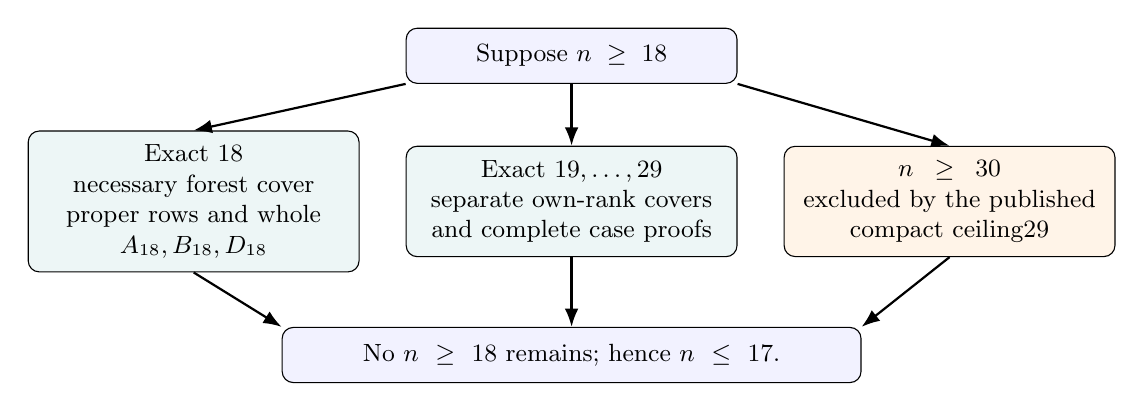
\begin{tikzpicture}[font=\small,>=Latex,
 box/.style={draw,rounded corners,align=center,text width=3.85cm,
 minimum height=1.4cm,inner sep=5pt}]
 \node[box,minimum height=.7cm,fill=blue!5] (start) at (6.7,3.85)
   {Suppose \(n\ge18\)};
 \node[box,fill=teal!7] (eighteen) at (1.9,2.0)
   {Exact \(18\)\\necessary forest cover\\proper rows and whole\\
    \(A_{18},B_{18},D_{18}\)};
 \node[box,fill=teal!7] (tail) at (6.7,2.0)
   {Exact \(19,\ldots,29\)\\separate own-rank covers\\and complete case proofs};
 \node[box,fill=orange!9] (published) at (11.5,2.0)
   {\(n\ge30\)\\excluded by the published\\compact ceiling29};
 \node[box,text width=7.0cm,minimum height=.7cm,fill=blue!5]
   (finish) at (6.7,.05)
   {No \(n\ge18\) remains; hence \(n\le17\).};
 \draw[->,thick] (start.south west)--(eighteen.north);
 \draw[->,thick] (start)--(tail);
 \draw[->,thick] (start.south east)--(published.north);
 \draw[->,thick] (eighteen.south)--(finish.north west);
 \draw[->,thick] (tail)--(finish);
 \draw[->,thick] (published.south)--(finish.north east);
\end{tikzpicture}
\caption{The complete compact conjunction. Within each case the original
farthest vertex and its vector stay fixed; a cover lists necessary forests,
not realized examples. The higher-rank proofs are independent of exact18
and use no face-inheritance or arithmetic premise. Their complete join is
Section~\ref{app:tail:completeconjunction}.}
\label{fig:ill20261026:c17:conjunction}
\end{figure}
% END ILLUSTRATION_20261026_C17_CONJUNCTION
\section{Finite algorithms and conditional verification}
\label{sec:verification}
\subsection{The mathematical finite-cover calculation}
The rank covers are finite combinatorial arguments supported
by real inequalities, not field enumerations.
For fixed total rank \(n\), the forest calculation is:
\begin{enumerate}
\item List partitions of \(n\) into ranks of spherical irreducibles.
 Retain all exceptional finite types and classical types at
 their actual ranks. Keep \(I_2(m)\) as a symbolic ordinary
 rank-two family for unbounded \(m\), distinguishing its
 exceptional actual typed profiles.
\item Mark at most one allowed \(I/J/N_7/O_7\) profile by the
 actual-wall compatibility lemma. Apply joint bounds only to
 disjoint sets of components, counting each defect once.
\item Sum proved same-vector energy bounds. Discard a forest only
 when a strict lower bound is at least \(1\). If a dominant
 rank needs a fresh local layer, retain it until that
 actual-rank lemma is established.
\item Return the retained grouped necessary cover and the
 inequality discarding every other partition.
\end{enumerate}
Termination follows from finitely many rank partitions and
finite type choices at each rank. The unbounded native
parameter is represented by inequalities proved over its
entire domain. Completeness uses spherical classification,
compact acute simplicity, complete actual-defect compatibility,
and spectator-uniform component bounds. The output is a
necessary cover; no realization follows. A program testing
only finitely many native labels would not establish it.

Local own/white calculations have a different domain.
After deleting a specified original node, classify every
finite extension of the retained spherical forest by its
actual opposite wall, including own zero, all finite owns,
parallel and dotted owns. Finite white extensions are bounded
by spherical classification. Infinite own families are closed
by analytic inequalities over complete intervals.
Termination of a finite classification does not justify
discarding a continuous branch. Completeness must include
spectator attachments, affine kernels and every original
wall for every auxiliary point.

\subsection{The distinct role of scripts}
The final continuous seals are proved by displayed rational
inequalities and calculus arguments. Ancillary scripts can check
finite arithmetic tables, but their execution records are separate
from the geometric arguments that make those tables applicable.

For a reproducibility checker attached to a finite table,
its mathematical statement must specify the exact input
domain, symbolic own parameters, exhaustive loops or recursion,
the terminating measure, exact tests and returned cover.
Its correctness proof must map every admissible geometric
case to a generated entry and each rejected entry to a
valid exclusion. The execution record then states what
that particular program returned on those inputs.
Algorithm theorem, execution claim and geometric consumer
are distinct. Historical receipts identified in the ledger
are not a new complete replay of this revision.

\subsection{The formal boundary}
A suitable Lean kernel may take as explicit parameters:
\begin{enumerate}
\item precise finite/affine classification and compact acute
 geometry statements supplied from the literature;
\item precise internal component and local-cap statements whose
 full written project proofs have been reviewed;
\item a precisely typed necessary-cover output, if exact
 enumeration is provided as a conditional premise.
\end{enumerate}
It may verify rank sums, disjoint-cover subtraction,
one-vector algebra, rational implications and the final
composition giving \(n\leq17\).
An internal geometric statement remains an internal proof
obligation when used as a parameter; it does not become
a literature theorem. Logic maps must list parameters as
well as printed axioms.

The supplementary Lean sources express selected algebraic and
discrete implications with explicit premises. Their logic maps list
the geometric, analytic, classification and finite-data statements
left outside each kernel. These conditional deductions are not a
formal construction of a hyperbolic polytope or a formalization of
every geometric lemma. Separate compilation and actual axiom-audit
records document the scope of each checked module.

\appendix

\section{Ordinary component proofs and actual defects}
\label{app:ordinary}
Throughout the proof appendices, \(F(t)=2t/(1+t^2)\) denotes
the full-/half-tangent conversion.
This appendix collects the contact calculations behind the small-component
rates. Each is an argument on an actual whole component with arbitrary
finite spectators, using Section~\ref{sec:geometry}. No field condition
is present. We use the spherical/affine classification and the standard
Lann\'er classification: a minimal indefinite Coxeter diagram with all
proper subdiagrams positive definite has at most five vertices.
A positive affine principal is already impossible by the actual null
argument in Section~\ref{sec:geometry}.

\begin{proposition}[Ordinary costs and the complete small defects]
\label{app:prop:ordinary}
All the ordinary component bounds in Section~\ref{sec:components}
hold with arbitrary finite spectators. For the moment use the weaker
bound \(B_3,H_3>1/4\); the improvement to \(2/7\) is proved immediately
below. The only exceptions to the rank-over-\(14\) small-component
baseline are one possible isolated short \(I\), its separately funded
\(J\) alternative, or one of the two typed rank-two defects.
\end{proposition}
Write \(m@j\) for actual contact \(\cos(\pi/m)\) at old node \(j\).
A missing contact is zero. For a wall put \(h=A^2\), own cost
\(q\) and full foreign cost \(Q\), so \(h=q+Q-1>0\).
The following calculations prove the proposition; their tables are
finite mathematical case analyses rather than empirical output.

\begin{lemma}[Common-wall forcing and isolation]\label{app:lem:ordinaryforcing}
Suppose the energy of a component is at most $e$. A pair for which
the right side of \eqref{eq:pairupper} is below $K_{ij}$ has one
actual opposite. If one wall closes every direction of the component,
then, with $v_i=(C\beta)_i/\sqrt{d_i}$ and
$R_e^2=4e/(1+e)^2$,
\begin{equation}\label{app:eq:commoncost}
 q-1\le h\le R_e^2\min_i v_i^2.
\end{equation}
If $h<1/4$, it has no foreign contact. In a path, a wall closing
every direction can have multiple contacts only at the two endpoints;
in a $D_4$ star it has at most one.
\end{lemma}
\begin{proof}
The first assertion is \eqref{eq:pairupper}. For a closed direction,
$\tanh L_i=A/v_i$ and $\tau_i^2\le e$, which gives
\eqref{app:eq:commoncost}. Every nonzero foreign cost is at least $1/4$
and is strictly below $h$ by \eqref{eq:foreigncost}; hence the isolation
assertion. If the old path between two contacts omits a direction
closed by the wall, deleting that direction leaves a cycle in an
actual finite replacement. This is impossible. The same argument
applies to every two contacts in a $D_4$ star. Finally, a single-contact
own cost $q=1$ gives an affine principal set, impossible even in the
presence of further spectators.
\end{proof}

\subsection{The short directions and their exact debits}

For a short $A_1$ opposite put $b=\beta^2$, $h=A^2$, and let $Q$
be its full foreign cost. Then
\[
 h=b+Q-1,\qquad h<b/3,\qquad Q<1-2b/3.
\]
Equation~\eqref{eq:foreigncost} rules out two foreign components.
With one, its cost must be the sole value below $1/3$, namely an
$A_1$ contact $3$ of cost $1/4$. Thus the only possibilities are
\[
 I:\ \hbox{isolated dotted }A_1,\quad 0<h<1/2;
 \qquad
 J:\ \hbox{dotted }A_1+A_{1,3},\quad 1/3<h<3/8.
\]
For completeness, with one foreign component,
$Q<h=b+Q-1$ forces $b>1$, and $Q<1/3$ then forces $Q=1/4$.
For $J$, the heavy edge contributes more than $A/2$ to
$x\cdot v$. The light shadow contributes at least
$A(1-\sqrt{1-1/(4h)})$; this is at least $A/2$ if $h\le1/3$.
Strict \eqref{eq:actualinterior} therefore gives the asserted lower bound.
Native acuteness excludes two short walls. Indeed their height
product is below $1/2$, so their product must be zero. Disjoint
supports give a negative product, heavy overlaps give a spatial
product above $1/2$, and a sole light/light overlap of two $J$ walls
gives $1/4$, below their height product. None is zero. A $J$ heavy
direction has $\tanh^2L>4/13$, hence energy $>9/100$; its light
direction has $\tanh^2L>2/3>16/25$, hence energy $>1/4$.
Thus $J$ funds both $A_1$ factors above their combined ordinary
baseline $2/10$. Every nonshort direction pays at least
$5-2\sqrt6>1/10$, since $\sqrt6<49/20$. We may conservatively
discard the one short direction, but only the isolated type $I$
can create an unfunded debit.

The rank-two exceptions are
\begin{equation}\label{app:eq:defects}
\begin{array}{c|c|c}
\hbox{old block / new isolated contact} & h=A^2 & \hbox{energy}\\ \hline
A_2/7 & (4/3)\cos^2(\pi/7)-1\in(0,1/12) & >9/100\\
I_2(7)/3 & (1/4)\csc^2(\pi/7)-1\in(0,1/3) & >9/100.
\end{array}
\end{equation}
Their spatial supports lie entirely in their own blocks.
Two defects in different blocks, or a defect and a short $A_1$,
would have actual wall product $-\sqrt{h_1h_2}\in(-1/2,0)$.
That interval is forbidden: distinct acute unit walls have product
$0$ or at most $-1/2$. Therefore
\begin{equation}\label{app:eq:debits}
\text{at most one short }A_1,\quad\hbox{or one rank-two defect,
but never both.}
\end{equation}
This argument is independent of every other component type.

\subsection{The two rank-two estimates}

For $A_2$, set $e_2=319/2000$ and $\sinh^2L_0=31/50$.
If both edges have length at least $L_0$, then their half-tangents
exceed $173/500$ and energy is greater than
$4\cdot173^2/(3\cdot500^2)>e_2$. A shorter edge cannot have two
positive own contacts: $3/3$ is affine, while $3/4$ or larger gives
$\sinh^2L\ge4\sqrt2/9>31/50$, increasing with either contact
and with $Q$. If only the other node is contacted, apply the same
test to that shorter contacted direction. For one contact of square
$b$, the shorter-edge condition is
\begin{equation}\label{app:eq:A2short}
 h=4b/3+Q-1<124b/243,\qquad Q<1-200b/243.
\end{equation}
Every positive foreign cost must be below $h$. A label $3$ gives
$h<1/4$, hence isolation and negative height. For a label $4$,
$h<62/243$ forces each foreign cost to be $1/4$; the only positive
possibility is $Q=1/2$, but then $h=1/6<1/4$. A label $5$ has
$Q<1/2$, hence at most one foreign component, whose cost exceeds
$h$ because its own cost $\ph^2/3$ is below one. A label $6$ is
affine. For a finite label $m\ge7$, $b>.81$ gives $Q<1/3$;
thus $Q=0$ or $Q=1/4$. The latter is possible in
\eqref{app:eq:A2short} only for $b<729/800$, namely $m=7,8,9,10$.
Indeed $\cos^2(\pi/11)>45/49>729/800$, using $\pi<22/7$.
A dotted contact has $Q<1/4$ and is isolated.

For an isolated finite contact the same wall closes the mate,
since its reciprocal ratio squared is $b/(4b-3)>1$.
For $m\ge8$ that actual mate has
$\tanh^2L\ge6\sqrt2-8>400/841$, so its energy exceeds
$4/25>e_2$. For an isolated dotted contact,
$b<243/200$ and its distinct mate has shadow
$\tanh^2L\ge b/(4b-3)>81/124>16/25$.
For a mixed $m=7,8,9,10$ contact, the mate's white cost is
$b+1/4>1$; the distinct shadow instead gives
$\tanh^2L\ge b/(4b-9/4)>11/17>16/25$.
Both give energy greater than $1/4$. Thus the only exception is
isolated new $7$ at old $A_2$.
The root $t=\cos(2\pi/7)$ of $8t^3+4t^2-4t-1$ lies in
$(623/1000,5/8)$: the polynomial changes sign there and is increasing
on $[1/2,1]$. Hence $b>1623/2000$ and its actual mate satisfies
$\tanh^2L=4-3/b>164/541>3600/11881$, proving its cost $>9/100$.

For an old $I_2(m)$, $m\ge4$, put $k=\cos(\pi/m)$ and
$d=(1-k^2)^{-1}$, so $C=d\left(\begin{smallmatrix}1&k\\k&1\end{smallmatrix}\right)$.
At energy at most $1/7$, \eqref{eq:pairupper} forces one common
opposite. Two contacts give an actual
$\cosh L\ge\cot(\pi/(2m))/\sqrt3>11/8$, with individual energy
$>3/19>1/7$. For one contact $\beta$,
\begin{equation}\label{app:eq:dihedralcut}
 q(1-7k^2/16)\le1,\qquad q=d\beta^2.
\end{equation}
Its minimum left side is $(9d+7)/64$. Since
$m\ge8$ gives $d\ge4+2\sqrt2>19/3$, only four old labels remain:
\[
\begin{array}{c|l}
m&\text{consequence of \eqref{app:eq:dihedralcut}}\\ \hline
4&\beta^2\le16/25<\cos^2(\pi/5):\ 3,4;\ h\le7/32<1/4,\ q\le1;\\
5&d>25/9:\ \text{only }3;\ h<7/32,\ q<1;\\
6&\text{only }3;\ q=1;\\
7&d>5:\ \text{only }3;\ Q<3/16.
\end{array}
\]
Isolation or the affine principal excludes the first three rows.
The last is isolated new $3$ at old $I_2(7)$, with $0<h<1/3$.
Its actual mate has $\cosh L=\cot(\pi/7)/\sqrt3>109/91$ by the
same cubic bracket; the squared comparison has positive numerator
$2652$. Thus its energy also exceeds $9/100$, completing
\eqref{app:eq:defects} and \eqref{app:eq:debits}.

\subsection{Rank three and four: one common-wall calculation}

For energy $1/4$, adjacent correlation at least $1/\sqrt3$ forces
a common opposite: the lowest cleared comparison is
$74/\sqrt3>39$. At energy $1/3$ the threshold $1/\sqrt2$ works,
since $51/\sqrt2>34$. For $A_4$ at energy $2/7$, the adjacent
correlations are $\sqrt{3/8},2/3,\sqrt{3/8}$; the forcing test is
$k^3+16k^2+36k-28>0$, whose lowest value is positive because
$291\sqrt6>704$. Direct inversion verifies the indicated
correlation thresholds for $A_3,B_3,H_3$ and $B_4,D_4,F_4$.
For $H_4$ use energy $11/36<1/3$. Thus a common wall closes all
directions in every case.

Number path bonds as $A_3:(3,3)$, $B_3:(4,3)$, $H_3:(5,3)$,
$A_4:(3,3,3)$, $B_4:(4,3,3)$, $F_4:(3,4,3)$, and
$H_4:(5,3,3)$. By Lemma~\ref{app:lem:ordinaryforcing}, multiple
contacts can only be at the endpoints. Two endpoint $3$ contacts
in $A_3,A_4$ are affine; the next minimum is $3/4$. In the other
rows below even $3/3$ is excluded. The displayed values are lower
bounds for $q-R_e^2v_j^2$, contradicting \eqref{app:eq:commoncost}:
\[
\begin{array}{c|c|c}
T&j&\text{lower bound}\\ \hline
A_3&2&177/200+9\sqrt2/100>1\\
A_4&2&(230+15\sqrt2)/243>1\\
B_3&2&(77+18\sqrt2)/100>1\\
B_4&3&15/16+\sqrt2/8>1\\
F_4&2&15/16+\sqrt2/4>1\\
H_3&2&(72\ph+95)/100>1.
\end{array}
\]
$D_4$ already has at most one contact. In $H_4$, two endpoint
contacts retain, after deleting old node $4$, a path at least
$(3,5,3)$ of determinant $(5-4\ph)/16<0$. Hence all contacts
are single.

For a single contact at $j$ let
$\sigma_j=\min_i(v_i^2/q)$. Formula \eqref{app:eq:commoncost} gives
$q\le(1-R_e^2\sigma_j)^{-1}$. The complete inverse calculation
is as follows; entries are in path order, and $D_4$ means leaf,center.
\begin{center}\small
\begin{tabular}{ccll}
\toprule
$T$&$d_j$&$\sigma_j$&upper $q$\\ \midrule
$A_3$&$3/2,2,3/2$&$1/9,1/3,1/9$&$225/209,75/59,225/209$\\
$A_4$&$8/5,12/5,12/5,8/5$&$1/16,1/6,1/6,1/16$&$162/155,243/215,243/215,162/155$\\
$B_3$&$3,4,2$&$1/3,1/2,1/3$&$75/59,25/17,75/59$\\
$D_4$&$2,4$&$1/4,1/2$&$16/13,8/5$\\
$B_4$&$4,6,4,2$&$1/4,1/3,1/2,1/4$&$16/13,4/3,8/5,16/13$\\
$F_4$&$4,12,12,4$&$1/2,2/3,2/3,1/2$&$8/5,2,2,8/5$\\ \bottomrule
\end{tabular}\end{center}
Here $R_e^2$ is respectively $16/25$, $56/81$ for $A_4$, and
$3/4$ for the $1/3$ rows. Dividing the upper $q$ by $d_j$
gives the finite native lists:
$A_3$ endpoints $3/4/5$, middle $3/4$;
$A_4$ endpoints $3/4$, inner $3$;
$B_3$ nodes $3;3;3/4$;
$D_4$ leaf $3/4$, center $3$;
$B_4$ nodes $3;\varnothing;3;3/4$;
$F_4$ endpoints $3$, inner $\varnothing$.
Each has $q\le1$. Equality is affine; in every other listed case
\eqref{app:eq:commoncost} gives $h<1/4$ (the largest needed bounds are
$16/75,7/155,28/405,3/16$). Isolation then gives $h=q-1<0$.
This proves the six crystallographic and $A$ rows.

For $H_3$, the minimum contact $\beta=1/2$ at node $1$ or $2$
gives tests at node $3$ equal to
$(199\ph+263)/500$ and $(61\ph+77)/125$, both above one.
At node $3$, $\beta\ge1/\sqrt2$ gives the test at node $1$
at least $(27\ph+118)/150>1$. Only $3@3$ remains, with
$q=(\ph+2)/4<1$ and $h\le4\ph^4/75<\ph/4$.
No spectator gives negative height; one has cost $Q>h$; two have
$Q\ge1/2$ and hence $h\ge q-1/2=\ph/4$. All are impossible.
For $H_4$, $R_e^2=1584/2209$; at $\beta=1/2$ the four tests
(contact node, test direction) are
\[
(1,4):\frac{4938\ph+3688}{2209},\quad
(2,4):\frac{7209\ph+5334}{2209},\quad
(3,1):\frac{2500\ph+2667}{2209},\quad
(4,1):\frac{625\ph+1219}{2209}.
\]
All exceed one, the last by $\ph>198/125$; larger contacts only
increase these positive tests. This proves $H_4>11/36$.

\subsection[The two intermediate A components]{The two intermediate \texorpdfstring{$A$}{A} components}

Use $C_{ij}=2\min(i,j)(N-\max(i,j))/N$, with $N=6,7$.
For $A_5$, distinct $2/3$ and $3/4$ pairs each demand a sum above
$109/100$. The vector $u_2+2u_3+u_4$ has square
$7+4\sqrt2<443/35$, and
\[
(109/50)^2-(3/8)(443/35)=209/35000>0.
\]
For $A_6$, the three pair demands are
\[
2249/2000,\qquad11547/10000,\qquad2249/2000;
\]
the vector $u_2+2u_3+2u_4+u_5$ has square
$<33781/1250$, with demand $34037/10000$ and Cauchy gap
$2181583/700000000$ at energy $3/7$.
These pair bounds follow by substitution in
$F(s/2)^2<K$. Thus a common $2/3$ occurs for $A_5$, and a common
$2/3$ or $3/4$ for $A_6$, up to reversal.

Each retained path allows one contact. The full two-contact list is
\begin{center}\small
\begin{tabular}{lll}
\toprule
Component/pair&positions&necessary finite-white labels\\ \midrule
$A_5,2/3$&$1,3$&$3/3$ or $4@1+3@3$\\
&$1,4;1,5;2,4;2,5$&both $3$\\
&$2,3$&both in $3,4,5$\\
$A_6,2/3$&$1,3$&$3/3$ or $4@1+3@3$\\
&$1,4;1,5;1,6;2,4;2,5;2,6$&both $3$\\
&$2,3$&$3,4,5$ at $2$; $3,4$ at $3$\\
$A_6,3/4$&$3,4$&both in $3,4,5$\\
&other eight left/right pairs&both $3$\\ \bottomrule
\end{tabular}\end{center}
Indeed deletion of either closed node leaves a connected finite
path or $D/E_6$ tree: a $4$ can only be terminal, and $D/E$ bonds
are all $3$. All-$3$ doubles are affine cycles. The adjacent
non-$3/3$ doubles force an actual edge of cosh at least
$(3+\sqrt2)/2>11/5$ in $A_5$; for $A_6$ the minimum formulas are
$(5+4\sqrt2)/\sqrt7$, $(4\sqrt2+6)/\sqrt{14}$, and
$(12+9\sqrt2)/\sqrt{42}$, all above $5/2$.
The $A_5$ terminal-$4$ row has $Q=0$ and cosh
$(3+\sqrt2)/2$. The $A_6$ version has white cost $9/10$, hence
$Q=0$, and is treated below. These cosh thresholds imply individual
energies above $3/8$ and $3/7$.

For single $3$ contacts the complete own costs and strict white
bounds are
\[
\begin{array}{c|c|c|c}
\text{component/pair}&j&q&Q\text{ upper}\\ \hline
A_5,2/3&1,2,3,4,5&5/12,2/3,3/4,2/3,5/12&2/3,2/3,5/8,1/2,5/8\\
A_6,2/3&1,2,3,4,5,6&3/7,5/7,6/7,6/7,5/7,3/7&2/3,2/3,3/5,2/5,2/5,3/5\\
A_6,3/4&1/6;2/5;3/4&3/7;5/7;6/7&5/8;1/2;5/8.
\end{array}
\]
End and small-$Q$ rows have $h<1/4$, or only one foreign
component with cost $Q>h$. In $A_5$ at $j=2,3$ two foreign
components would each exceed $1/3,1/4$, respectively, forcing
$Q\ge2/3$; the same gap treats $A_6,j=2$.
In the remaining $A_6,j=3,4$ rows, two foreign bonds must be $3$
since $Q<5/8$; together with the contacted old node and its two
neighbors they form affine two-fork $D_5$. This excludes all single
$3$ cases. A single internal $4$ gives the affine $(3,3,4)$ star;
an end $4$ has $Q\le1/3$ and $h<1/4$, again impossible.

A single $5$ is at a retained path end; its $H_3/H_4$ white cost
exceeds $3/4$, so $Q=0$. All cases are covered by these actual
positive replacements:
\[
\begin{array}{c|c|c|c}
\text{component/pair}&\text{contact}&\text{actual direction}&\cosh L\\ \hline
A_5,2/3&1\text{ or }5&4\text{ or }2&\ph^3/\sqrt3\\
&2&3&\ph^2\\
&3&2&\sqrt3\ph^3\\
A_6,2/3&1&4&3\ph^3/\sqrt{21}\\
&2&3&4\ph^2/\sqrt{14}\\
A_6,3/4&1\text{ or }6&4\text{ or }3&3\ph^3/\sqrt{21}\\
&3\text{ or }4&4\text{ or }3&9\ph^3/\sqrt{21}.
\end{array}
\]
The first group exceeds $11/5$, the second $5/2$, using
$\ph>8/5$, $\sqrt{21}<23/5$, $\sqrt{14}<15/4$.
No new wall is inferred: each replacement contains the already
actual $c$. Finally the $A_6$ double $4@1+3@3$ has the positive
actual future point
\[
 \xi=c+(\sqrt2-1/2)n_1+(\sqrt2-1)n_2+(\sqrt2/2)n_3,
 \qquad \xi^2=5/4-\sqrt2=-k.
\]
Its products with $c,n_1,n_3$ vanish and its product with $n_2$
is $(\sqrt2-3)/4<0$. Here $A^2=(5+4\sqrt2)/7$ and
$A^2-9k=(335-236\sqrt2)/28>0$; \eqref{eq:pointenergy} gives
energy $>(A-\sqrt k)/(A+\sqrt k)>1/2$.

\subsection[The four intermediate B components]{The four intermediate \texorpdfstring{$B$}{B} components}

Use $u_i=(e_1+\cdots+e_i)/\sqrt i$ and, for $i<r$,
$\omega_i=\sqrt2(e_1+\cdots+e_i)$, while
$\omega_r=e_1+\cdots+e_r$.
At energies $3/7,1/2,4/7$ the relevant forcing signs are
$127\sqrt{2/3}-100$, $(69\sqrt{6/7}-52)/7$, and
$(199\sqrt{6/7}-176)/7$, all positive.
Thus $B_5,B_6$ have a common $2/3$, and $B_7,B_8$ a common $6/7$.

For $B_5,B_6$, deletion $2$ retains $A_1+B_3/B_4$.
The right contact is $3@3$, with the sole $B_5$ exception $3@5$
giving $F_4$; deletion $3$ allows one left $3/4/5$.
For $3@3$, own $0$ is affine, own $3$ is a triangle, and own
$\ge4$ gives $\cosh L_3\ge2+3/\sqrt2>3$.
With no right contact the complete choices are $3/4/5$ at $1$ or
$2$: $3@2$ and either $4$ are affine; $3@1$ has
$h=Q-1/2<1/6$ and closes a forbidden foreign direction.
The two $5$ cases have $Q=0$: $5@1$ also closes $4$ with
$\cosh L_4=\ph^3>3$, and $5@2$ has
$\cosh^2L_3=2\ph^2/(2-\ph)>9$.
For the $B_5$ short-end $3@5$, finite $F_4$ forbids left $1$
and all spectators; own $0$ is affine and the other replacement
forces own $3$, giving $\cosh L_2=2+\sqrt2$.
Every branch exceeds the individual threshold $11/5$.

For the $6/7$ pair, a wall without a right contact has a single
left $3$ or endpoint $4$. Apart from far $3@1$ these give an
affine fork, double-$4$, or star. A minimal nonpositive principal
for the far branch must contain $c,7$, since deletion $7$ is
finite; their connecting path $c,1,\ldots,7$ has eight vertices.
Spectators attach through $c$ and do not shorten it. This violates
the Lann\'er order bound, excluding the branch with all spectators.
In $B_7$, let $\beta$ be the contact to the retained right $A_1$:
\[
\begin{array}{c|l|l}
\beta/\text{own }6&\text{left contacts}&\text{pressure or rejection}\\ \hline
\beta\ge\cos(\pi/5),\ \text{any}&\text{none}&\cosh L_6\ge\sqrt6\cot(\pi/5)>3\\
\beta_4,0&\text{any allowed}&\text{affine }(4,4)\\
\beta_4,>0&\text{none}&\cosh L_6\ge\sqrt{24}\\
\beta_3,>0&\text{none}&\cosh L_6\ge2+\sqrt2\\
\beta_3,0&\text{none or }1&\text{affine }F_4\\
\beta_3,0&\text{one }j=2,\ldots,5&\cosh L_6\ge1+3/\sqrt2>3.
\end{array}
\]
Here $\beta_m=\cos(\pi/m)$. The last row retains the full foreign
cost: its white residual is
$\Delta\le3/4-j(6-j)/12\le1/3$, and
$v_6\ge\sqrt{12}(j/12+1/(2\sqrt2))$.
Thus no allowed $E_7$ extension is silently removed.

In $B_8$ the retained right $B_2$ has one simple $3$ at either
end. At long end $7$, own $0/3$ is affine and own $4$ gives
$\cosh L_7\ge6+7/\sqrt2>7$.
At short end $8$, own $>0$ gives
$\cosh L_6\ge\sqrt6+\sqrt3>11/3$.
At own $0$, the left-white budget permits only $3@1$ or $3@5$:
none or $1$ gives affine $F_4$, but $3@5$ is an allowed bridge,
with $\Delta\le1/12$ and
$v_6=\sqrt{12}(5/12+1/(2\sqrt2))$.
It has $\cosh L_6\ge5+3\sqrt2>9$; it is estimated, not removed
by an incorrect $F_4$ sealing claim. These complete lists prove
the four asserted $B$ costs.

\subsection[Extended stars, D7, and the D8 closure]{Extended stars, \texorpdfstring{$D_7$}{D7}, and the \texorpdfstring{$D_8$}{D8} closure}

Let $S$ be a central $D_4$ star with an extended arm. If one wall
closes its center and three neighbors, every minimal nonpositive
principal contains $c$ and all four nodes of $S$, since deletion
of any of them is an actual finite replacement. Compactness and
the Lann\'er order bound make that principal exactly $S+c$.
Two contacts give a nonpositive proper triangle or cycle.
A sole center $3$ is affine, and a larger center contact has a
nonpositive proper star. A sole leaf contact is $3/4/5$ from its
finite proper path: $3$ gives finite $D_5$, $4$ affine, leaving
only $5$. If that leaf extends, it retains a nonpositive $(5,3,3)$
star; if another arm extends, it retains a nonpositive $(5,3,3,3)$
path. Each omits a supposedly closed $S$ direction, a contradiction.
Further negative contacts cannot repair the positive nonpositive
quadratic witness. Thus the four opposites cannot all coincide.

For $D_5,D_6$ the minimum central correlations are
$\sqrt{3/5},\sqrt{2/3}$. At energies $5/14,3/7$ the forcing
signs are $544\sqrt{3/5}-362$ and $127\sqrt{2/3}-100$, positive.
For $E_6,E_7,E_8$ the arm lengths are $(1,2,L)$ with $L=2,3,4$.
In raw norm-two coordinates the central Schur residual is
$\delta=2-[1/2+2/3+L/(L+1)]$; on an arm of length $m$, squared
central correlation is $t/(\delta+t)$, $t=m/(m+1)$.
The minima are $\sqrt3/2,\sqrt{6/7},\sqrt{15}/4$.
At energies $9/20,5/9,2/3$ even $4e/(1+e)^2$ lies below these
correlations. All four opposites would coincide, proving the five
extended-star costs.

For $D_7$ write $o=r-2$, $a=r-3$, with fork leaves $b,f$.
At energy at most $1/2$, correlation $\sqrt{4/5}$ forces a
common $o,a$. Deletion $a$ retains $A_3=b-o-f$, so its right
contact is none, middle $3$, or endpoint $3/4/5$; deletion $o$
allows one left contact. The complete surviving profiles are
\begin{equation}\label{app:eq:D7roles}
 4@a+3@o,\qquad\text{isolated }5@b,\qquad3@a+4@b,
\end{equation}
up to exchanging the fork leaves. To check the list: middle $3$
forces $4@a$ (own $0/3$ is affine); endpoint $5$ seals all white
extensions by $H_4$, and a contact at the removed $a$ leaves a
nonpositive $(3,3,3,5)$ path. Endpoint $4$ forces $3@a$, otherwise
an affine terminal-$4$ fork remains. Endpoint $3$ excludes every
left contact by cycles or retained $F_4$; a foreign $3$ is affine
$E_7$, a foreign $4$ is an affine terminal-$4$ fork, and larger
foreign bonds are nonfinite. Its isolated height is negative for
$r=7$ and it contains affine $E_8$ for $r\ge8$.
With no right contact, internal-left $3$ and endpoint $4$ are
affine; far-left $3$ needs a Lann\'er path of at least six vertices.
This accounts for all spectators as well as the removed own contact.
The first and third roles have
$\cosh L_o=a+(r-2)/\sqrt2>7$.
The isolated $5$ has
$\tanh^2L_a=1-(9-4\sqrt5)/(r-3)$; at $r=7$ its half-tangent
square is $4/\sqrt5-1>3/4$. Each role therefore contradicts
energy at most $1/2$, proving the $D_7$ cost.

For $D_8$, common $4/5$ has exactly $4@4+3@5$.
Indeed deletion $4$ permits simple $3$ at a right $D_4$ leaf,
and deletion $5$ allows one left $3$ or endpoint $4$.
Long-leaf $3$ forces $4@4$ and forbids foreign contacts by the
retained $(3,4,3,3)$ path. A fork $3$ with a left $3$ gives an
affine cycle; without a left contact it is affine $E_8$; a left
$4$ is nonpositive. With no right contact only far $3@1$ survives
the affine tests, but its path to $5$ has six vertices.
Common $5/6$ has the preceding center-neighbor list. Both common
pairs thus force an actual half-tangent square above $3/4$.
At energy at most $4/7$, their opposites are distinct.

Here is the remaining three-direction calculation. Put
$q=\sqrt{4/5}$, $k=\sqrt{5/6}$, $\lambda=(1+k)/2$,
$\alpha=k\sqrt{1-k}/2$, $e=4/7$, and
$P(t)=t/(1+\sqrt{1-t})^2$.
Write $h_i=x\cdot u_i$ and decompose
$x=aw+bv+zt_0+y$, where $w,v$ are the normalized sum and
difference of $u_5,u_6$, $u_4=qu_5+t_0/\sqrt5$, and
$y\perp w,v,t_0$. The full-tangent laws imply
\[
 h_4h_5\ge P(q),\qquad
 T:=(1+\alpha)b^2+\lambda z^2
 \le\delta:=\lambda e-P(k)<1/400.
\]
For the second inequality take the tangent line to
$4p/k-(1+p)^2$ at its first zero $p=P(k)$, with
$p=h_5h_6=\lambda a^2-(1-\lambda)b^2$.
Keeping the negative quadratic terms in $h_4h_5$ gives
\[
 h_4h_5\le q\lambda e+A_0|b|+B_0|z|
              -qkb^2-q\lambda z^2,\qquad
 A_0^2=8/105,\quad B_0^2=4/35.
\]
Weighted Cauchy bounds the linear part by $\sqrt{C_0T}$, where
$C_0=(8/105)/(1+\alpha)+(4/35)/\lambda<47/250$.
Also $qk/(1+\alpha)>.71$, $q>.71$, and $q\lambda e<.489$.
Consequently
\[
 h_4h_5<.489+\sqrt{(47/250)T}-.71T
 <101781/200000<.509<P(q),
\]
a contradiction. The rational seals are
$.8944<q<.8945$, $.9128<k<.9129$,
$.29<\sqrt{1-k}<.2953$, $.13<\alpha<.14$,
and $.95<\lambda<.95645$.
The tight $\delta$ comparison reduces to
$91280000\cdot70000-167780209\cdot38083=26300653>0$;
the last square-root comparison uses
$\sqrt{47/100000}<271/12500$.
This proves $D_8>4/7$ and completes Proposition~\ref{app:prop:ordinary}.

\subsection{The strengthened rank-three rates}
\label{app:strongrankthree}
We prove the improvement \(B_3,H_3>2/7\) used in the forest
accounting. Suppose the component energy is at most \(2/7\).
The adjacent correlations are at least \(1/\sqrt2\), so the
forcing argument above gives one actual opposite for the whole
component, with
\[
 h\leq R^2\min_i v_i^2,\qquad R^2=56/81.
\]
All foreign costs remain included in \(h=q+Q-1\).
Multiple contacts can occur only at the two path endpoints.

For \(B_3\), endpoint contacts \(u,w\) give
\[
 q-R^2v_2^2=(131u^2+106w^2+50\sqrt2uw)/81.
\]
If either label is at least \(4\), its minimum is \(13/9\)
or \(443/324\), both greater than \(1\). Larger contacts
increase the expression. At \(u=w=1/2,Q=0\), the actual
half-tangent squares in directions \(2,3\) are
\((2\sqrt2-1)/7\); increasing \(Q\) increases both lengths.
Their correlation is \(1/\sqrt2\), so the positive two-direction
cover costs at least \((10\sqrt2-12)/7>2/7\).
For one contact the diagonals are \(3,4,2\), with minimum
ratios \(v_i^2/q=1/3,1/2,1/3\). Thus the maximum own costs
are \(243/187,81/53,243/187\).
Nodes \(1,2\) admit only native \(3\), and node \(3\) only
\(3,4\), since \(243/374<\varphi^2/4\).
Every \(q=1\) case is affine; every remaining \(q<1\) case
has \(h<1/4\), forcing \(Q=0\) and \(h=q-1<0\).

For \(H_3\), the endpoint quadratic has positive coefficients;
its minimum at \(u=w=1/2\) is
\((200\varphi+287)/324>1\).
At node \(1\) or \(2\), even contact \(1/2\), tested in
direction \(3\), gives respectively
\[
 (599\varphi+823)/1620>1,\qquad
 (181\varphi+237)/405>1.
\]
At node \(3\), contact at least \(1/\sqrt2\), tested in
direction \(1\), gives \((75\varphi+374)/486>1\).
Only contact \(1/2\) remains, with
\[
 q=(\varphi+2)/4<1,\qquad h\leq14\varphi^4/243.
\]
No foreign component gives \(h<0\); exactly one is impossible
by \(Q<h\). Two or more give
\[
 h\geq q-1/2=\varphi/4>14\varphi^4/243,
\]
the final difference being \((75\varphi-112)/972>0\).
This covers all native/dotted contacts and all spectators.

\subsection[A rank-free joint payment for an isolated I]{A rank-free joint payment for an isolated \(I\)}
\label{app:Ijoint}
Let the actual isolated short wall be
\[
 c_0=\sqrt h\,p-\sqrt{1+h}\,e,\qquad0<h<1/2,
\]
with \(e\) the old unit \(I\) normal.
For an actual opposite outside \(I\), write its time as \(A\)
and its contact with \(e\) as \(\gamma\).
The finite white endpoint retains \(e\), so \(\gamma=0\)
or \(1/2\leq\gamma<1\). These opposites are distinct.
For the chosen unit dual \(u\perp e\), its spatial derivative
has square at most \(1+A^2-\gamma^2\).
If \(\gamma=0\), the native gap gives \(A^2\geq1/(4h)\);
if \(\gamma>0\), acuteness gives
\(A^2\geq(1+h)\gamma^2/h\).
Since \(\gamma^2<1\), the derivative comparison yields in
both cases
\begin{equation}\label{app:eq:Ifulltangent}
 \tanh^2L\geq\frac1{1+4h}.
\end{equation}
For the nonzero case, substitute the lower bound on \(A^2\);
the difference from \(1/(1+4h)\), after positive denominators
are cleared, has numerator \(h((5+4h)\gamma^2-1)>0\).

Let \(q\) be the actual \(I\)-edge half-tangent square.
Then \(h=4q/(1-q)^2\), \(0<q<1/5\).
If \(\theta\) is the half-tangent square of the other edge,
the increasing function \(4s/(1+s)^2\) and
\eqref{app:eq:Ifulltangent} show \(\theta>1/5-q\).
The exact cross numerator for the strict comparison is
\[
 (1-q)^2(6-5q)^2-20(1-5q)(1+14q+q^2)
 =(39q-4)^2+q^2(40-10q+25q^2)>0.
\]
Thus the same original vector satisfies
\(e_I+\ip{x}{u}^2>1/5\).
For another whole \(A_1\) this proves \(I+A_1>1/5\);
adding a second ordinary \(A_1>.1\) proves \(I+2A_1>.3\).

For the sharper \(I+T_2\) bound set \(s=\sqrt q\in(0,1/3)\)
and \(t=\sqrt{1+4h}-2\sqrt h\).
Equation~\eqref{app:eq:Ifulltangent} gives normalized height
at least \(t\) in every other actual edge direction, and
\[
 e_I\geq s^2,\qquad(1-s^2)(1-t^2)=8st.
\]
We need \(t+\tfrac32s>.767\).
At \(t_0=.767-1.5s>0\), the left-minus-right of that relation is
\[
 P(s)=.411711-3.835s+9.338289s^2-2.301s^3+2.25s^4.
\]
Putting \(v=s-.2\in(-.2,2/15)\), its coefficients are
\(.00343456,-.3038044,8.497689,-.501,2.25\).
Its cubic term is at least \(-.0668v^2\), so
\[
 P(s)>.0034-.304|v|+8.43v^2>0,
\]
as the last quadratic has negative discriminant.
The original relation decreases strictly in positive \(t\),
proving the barrier. This is a scalar real argument; no
arithmetic chapter of its source is used.

The ordinary \(T_2\) energy is greater than \(1/7\).
If \(s\geq519/2000\), \(s^2+1/7>.21\).
Below that split, \(s^2+(.767-1.5s)^2\) decreases to
\(.2100353125>.21\). Thus \(I+T_2>.21\), counting \(I\) once.

For \(I+T_3>2/7\), \(B_3,H_3\) already have the intrinsic
stronger bound. For \(A_3\), if \(h>1/5\), the actual
\(I\)-edge gives \(e_I>3/70\), and
\(3/70+1/4>2/7\).
If \(h\leq1/5\), all three other half-tangent squares are
at least \(1/5\). The normalized \(A_3\) dual Gram \(K\)
has \(K^{-1}\mathbf1>0\) and
\(\mathbf1^TK^{-1}\mathbf1=5-2\sqrt3\);
positive Cauchy gives energy at least
\((5-2\sqrt3)/5>3/10>2/7\).
The same positive-cover principle will be used below:
if \(K^{-1}\mathbf1>0\) and every height is at least
\(\sqrt\theta\), energy is at least
\(\theta\mathbf1^TK^{-1}\mathbf1\).

\subsection{Propagation from each actual typed rank-two defect}
\label{app:typedpropagation}
For \(N_7\), put \(b=\cos^2(\pi/7)<5/6\) and
\(h_N=4b/3-1<1/12\).
An opposite in another component retains the whole old
\(A_2\), so has no contact there or one contact of white
cost \(q\in[1/3,1)\).
In the contact case its spatial product with the isolated
wall has square at least \(bq/3\).
Acuteness and the bound on the chosen derivative give
\[
 A^2\geq\frac{bq}{3h_N},\qquad
 \tanh^2L\geq\frac{b}{b+6h_N}
             =\frac{b}{9b-6}>\frac59.
\]
The first ratio is minimized at \(q=1/3\); all denominators
are positive. Without contact the native gap instead gives
\(\tanh^2L\geq1/(1+4h_N)>5/9\).
Every other half-tangent square therefore exceeds \(1/5\).
In particular another \(A_1\) or irreducible \(T_2\) has
energy greater than \(1/5\).

For \(O_7\), put \(d_7=\csc^2(\pi/7)\) and
\(h_O=d_7/4-1\in(0,1/3)\).
No opposite in another component can contact the retained
old \(I_2(7)\): its minimum white cost \(d_7/4>1\) violates
positive definiteness. Its actual product with the isolated
typed wall is thus \(-\sqrt{h_O}A<0\), and the native gap gives
\begin{equation}\label{app:eq:O7height}
 A^2\geq1/(4h_O)>3/4
\end{equation}
for every opposite in the other component.
This immediately gives another \(A_1\) cost \(>2/15\)
by the full-/half-tangent comparison in the main text.

To prove another irreducible \(T_2=I_2(m)\) costs \(>1/5\),
suppose the contrary. With \(k=\cos(\pi/m)\) and
\(d=(1-k^2)^{-1}\), distinct opposites are impossible:
for \(m\geq4\), their tangent product is at most
\(F(\sqrt{1/5})^2=5/9<k\); for \(m=3\), use the pair sum
bound to get \(F(\sqrt{3/20})^2=240/529<1/2\).
There is one common actual opposite, and both actual
edge cosines are at most \(3/2\).
For own contacts \(b,g\geq0\) and entire foreign cost \(Q\),
the finite endpoint equations are
\[
\begin{gathered}
 Q+b^2<1,\quad Q+g^2<1,\quad
 h=d(b^2+2kbg+g^2)+Q-1>3/4,\\
 C_b=\frac{\sqrt d(b+kg)}{\sqrt{1-Q-g^2}},\qquad
 C_g=\frac{\sqrt d(g+kb)}{\sqrt{1-Q-b^2}}.
\end{gathered}
\]
Every nonzero own is consequently a finite native cosine.
There is at least one, and \(Q=0\) or \(Q\geq1/4\).

If only \(b=\beta>0\), the mate has
\(C_g^2=1+h/(1-Q-\beta^2)\).
The bounds \(h>3/4,C_g\leq3/2\) force
\(Q+\beta^2<2/5\), hence \(Q=0,\beta=1/2\).
Then \(h=d/4-1>3/4\) implies \(d>7>d_8\), so \(m\geq9\).
But \(d>81/\pi^2>81/10>31/4\), giving
\(C_g^2=(d-1)/3>9/4\), a contradiction.

If both contacts are positive and \(Q>0\), either their
maximum is at least \(1/\sqrt2\), giving
\(C_b^2\geq2+4\sqrt2/3>9/4\), or both are \(1/2\).
For old \(m=3\), the latter gives \(h=Q<3/4\);
for \(m\geq4\), it gives
\(C_b^2\geq(1+k)/(2(1-k))>5/2\).
If both contacts are positive and \(Q=0\), a contact of
label at least \(5\) gives \(C_b^2>3\); two \(4\)'s give
\(C_b^2=(1+k)/(1-k)\geq3\).
For \(3/4\), old \(m\geq4\) gives \(C_b\geq2\),
while old \(m=3\) gives \(h=\sqrt2/3<3/4\).
For \(3/3\), old \(m\geq5\) gives
\(C_b^2=(1+k)/(3(1-k))>3\);
old \(m=3,4\) give \(h=0,1/\sqrt2<3/4\).
This exhausts all finite labels and all foreign costs,
contradicting the common-wall low-energy branch.
Thus \(O_7+T_2\) has its other component energy \(>1/5\).


\section[The uniform actual B/D component floor]{The uniform actual \(B/D\) component floor}
\label{app:BDfloor}
The next proof supplies the \(9/14\) input used before the long-prefix
argument. Its small boundary cases refer only to the complete ordinary
contact calculations in Appendix~\ref{app:ordinary}. All displacements
remain in the indicated component, and all positive actual-root
constructions retain every original spectator wall.

\begin{proposition}[Actual $B/D$ floor]\label{app:prop:BDnine}
Every whole $B_r$ or $D_r$ component with $r\ge9$ has actual
projection energy greater than $9/14$, with arbitrary finite
spectators.
\end{proposition}

\begin{proof}
Assume energy at most $e=9/14$. In $B$ it suffices to bound the first
seven coordinates; all displacements below lie there. The normalized
directions in either type are $u_i=(e_1+\cdots+e_i)/\sqrt i$.
We first establish distinctness of $4/5,6/7$, then use those laws to
exclude all common $1/2,2/3$ profiles. This order is noncircular.

For an internal common $i/(i+1)$ with right retained rank at least
four, finite classification permits a right long-leaf $3$, or none.
The first forces own $4$: own $0/3$ is affine fork/triangle, and
any foreign contact retains the nonpositive $(3,4,3,3)$ path.
Without a right contact, internal-left $3$ and endpoint $4$ are
affine. Only far $3@1$ remains, but its path to $i+1$ has at least
six vertices, contradicting the Lann\'er bound. Right $D$-fork
contacts give affine $E_8$ or a cycle with the left contact.
Thus the sole common profile is $4@i+3@(i+1)$, $Q=0$, with
$\cosh L_{i+1}=i+(i+1)/\sqrt2>7$.
The $D_8$ right-$D_4$ and center-neighbor boundary calculations are
in Section~\ref{app:ordinary}; the center-neighbor calculation also
handles $D_9$ at $6/7$.
In $B_9$, the extra right short-end $3@9$ gives $F_4$, excluding
left and foreign white contacts. The removed own $6$ remains to check:
own $0$ is affine $F_4$, own $4$ the affine $(4,3,3)$ star, and own
$3$ gives $\cosh L_6=(1+1/\sqrt2)\sqrt{12}>11/2$ and
$\tau_6^2>9/13>e$. Consequently $4/5$ and $6/7$ are distinct.

Write $h_i=x\cdot u_i$. Distinct $6/7$ gives
$h_6h_7\ge k/(1+\sqrt{1-k})^2>9/16$, where
$k=\sqrt{6/7}>576/625$ with squared margin $21318$.
Hence $x\cdot w>3/2$ for $w=u_6+u_7$.
We record four local tests with their exact margins.

\emph{Edge $2$ with $\cosh L_2\ge1+\sqrt2$.}
Then $h_2^2\ge\sqrt2-1$. Projection of $w$ about $u_2$ has
$\rho=1/\sqrt3+\sqrt{2/7}<1.114$ and residual square
$S=29/21+4\sqrt{2/21}<2.62$.
Its Cauchy envelope $\rho t+\sqrt{S(e-t^2)}$ decreases for
$t\ge q=\sqrt{\sqrt2-1}$: its derivative condition follows from
$\rho^2e<13/16<6/5<\|w\|^2q^2$.
Since $q<.644$, $e-q^2<.23$, and $\sqrt{2.62\cdot.23}<.777$,
$x\cdot w<1.114(.644)+.777=1.494416<3/2$.
These follow by squaring, using $1.414<\sqrt2<1.4143$,
$1/\sqrt3<.578$, $\sqrt{2/7}<.535$, $\sqrt{2/21}<.309$.

\emph{Isolated $5@1$.}
Its height square is $(\ph-1)/2$ and its actual direction-$4$
shadow has $\tau_4^2=\ph-1$. For the same $w$, projection about
$u_4$ has $\rho=2(1/\sqrt6+1/\sqrt7)<787/500$ and
$S=16/21+4/\sqrt{42}<69/50$. Use
$1/\sqrt6<.409$, $1/\sqrt7<.378$, $\sqrt{42}>162/25$;
the last residual comparison has cleared margin $23$.
Since $\sqrt e<401/500$, $e-(\ph-1)<1/40$ and
$(93/500)^2>69/2000$, Cauchy gives
$x\cdot w<362087/250000<3/2$.

\emph{Isolated $5@2$.}
Its height square is $\ph$. The direction-$1$ shadow gives
$x_1>31/50$, since $F(31/50)^2<161/200<\ph/2$ with cleared
margin $6541881$. Its actual edge $3$ has
$\cosh L_3=\sqrt2\ph^2>37/10$; hence
$S_3=x_1+x_2+x_3>131/100$, using
$3\tau_3^2>81/47>(131/100)^2$, of margin $3433$.
Distinct $4/5$ gives $x\cdot w_0>57/40$, $w_0=u_4+u_5$.
Put $v=e_1+e_2+e_3$, $k_0=1/2+1/\sqrt5<237/250$, and
$x_0=(31/50,69/200,69/200,0,\ldots)$.
Then $x_0=(11/40)e_1+(69/200)v$, $x\cdot x_0>x_0^2>31/50$.
The residual $w_0-k_0v$ has square $13/20+1/\sqrt5<11/10$
and excess demand $>9/50$.
All coefficients of $x_0+(w_0-k_0v)/6$ remain positive, and its
Cauchy margin is at least
\[
 (31/50+(9/50)/6)^2-e(31/50+(11/10)/36)=3/700>0.
\]

\emph{Contacts $4@2+3@3$.}
The white $A_2$ cost is $2/3$, so $Q=0$ or $1/4$; the latter has
$\cosh L_3=4+3\sqrt2>7$. At $Q=0$, put $s=\sqrt2$.
The actual floors satisfy
$\tau_2^2=(1+2s)/7$, $\tau_3^2=(2s-1)/3$,
$\tau_2\tau_3=1/\sqrt3$.
Their positive equality vector has $E_0=(6s-4)/7>.6407$.
The positive old-$A_2$ correction of $c$ is an actual future point
of square $-s/3$, giving pure displacement
\[
 U=\frac{2+s}{2}e_1+\frac{1+s}{3}(e_2+e_3+e_4),\qquad
 x\cdot U\ge A-\sqrt{s/3},\quad A^2=(5+4s)/2.
\]
Its projection coefficients on $u_2,u_3$ are
$\rho_2=(2s+1)/6$, $\rho_3=(1+s)/\sqrt3$;
its residual square is $(7+4s)/12<1.055$, with excess demand
$\Delta>.06$.
Indeed $1.4142<s<1.4143$ gives $A>2.3083$,
$\sqrt{s/3}<.6867$, $\tau_2\in(.7395,.7396)$,
$\tau_3\in(.7806,.7808)$, $\rho_2<.6381$, $\rho_3<1.394$,
and excess $>.06122604$.
The old positive coefficients exceed $.3,.52$; subtracting
$(\rho_2,\rho_3)/16$ removes less than $.04,.088$.
The corrected dual therefore has Cauchy margin at least
\[
 (.6407+.06/16)^2-e(.6407+1.055/256)
       =8825113/11200000000>0.
\]
This is an actual-point constraint, not an edge-only assertion.

Now exhaust common $1/2$. Deletion $1$ retains right rank at least
eight, so the right contact is none or long-leaf $3@2$.
The latter forces own $\gamma\ge1/\sqrt2$ (own $0/3$ is affine),
and $\cosh L_2=(1+\gamma)/\sqrt{1-\gamma^2-Q}\ge1+\sqrt2$,
already excluded. Without a right contact,
$A^2=2\gamma^2+Q-1>0$ and $\gamma^2+Q<1$.
Own $0$ has zero derivative; own $3$ has height below $1/4$ and
forces a foreign closure; own $4/6$ is affine.
Own $5$ with $Q>0$ has $\cosh L_2\ge\ph^2>1+\sqrt2$;
at $Q=0$ use the isolated-$5$ test. Finite $m\ge7$ forces $Q=0$;
$m\ge8$ uses the edge-$2$ test, leaving only isolated $7$.

For common $2/3$, deletion $2$ retains right $B/D$ rank at least
seven; deletion $3$ allows one left $3/4/5$ at $1$ or $2$.
A right long $3@3$ forces own $3/4/5$: own $0$ is affine, own $3$
a triangle, own $4$ is the tested $4+3$ profile, and own $5$ has
$Q=0$, $\cosh L_3=(2+5\ph)/\sqrt2>7$.
Without a right contact the full left list is
$3@1,4@1,5@1,3@2,4@2,5@2$.
The first has $A^2=Q-1/2<1/6$ and forces foreign closure;
$4@1,3@2,4@2$ are respectively affine terminal-$4$, two-fork,
and $(4,3,3)$ star. The $5$ cases have $Q=0$ by white cost
$\ph^2/3>3/4$ and were tested above.
For $D_9$ one extra right-fork $3$ gives retained $D_7+c=E_8$.
It excludes old-$1$ and foreign contacts, but the removed own $2$
must still be checked: own $0/3/4$ gives affine $E_8$/cycle/star,
and own $5$ retains nonpositive $(3,5,3)$. At higher rank the fork
attachment already contains affine $E_8$. No finite branch is omitted.

For the final isolated $7@1$, put $t=\cos(2\pi/7)$,
$g=\cos(\pi/7)$, and
\[
 \xi=c+g^{-1}n_1+(1-t)g^{-1}n_2
     =\sqrt t\,p-\frac V{\sqrt{1+t}},\qquad
 V=t(e_1+e_2)+(1-t)e_3.
\]
It has $\xi\cdot c=\xi\cdot n_1=0$,
$\xi\cdot n_2=(1/2-t)/g<0$ and
$\xi^2=-(1-t)(2t-1)/(1+t)<0$.
All coefficients and its time coefficient are positive, proving
actual feasibility and future orientation. Thus
$x\cdot V\ge\sqrt{t(1+t)}-\sqrt{(1-t)(2t-1)}$.
The increasing cubic $8t^3+4t^2-4t-1$ gives $.6234<t<.6235$,
with endpoint values $-.000926392768,.000105223$.
Hence the first radical is $>1.0059$, the second $<.305$,
and $.95<\|V\|<.9588<.959$, so $x\cdot\widehat V>.73$.
The projection of $w$ onto $\widehat V$ is
$\rho=(1/\sqrt6+1/\sqrt7)(1+t)/\|V\|\in(1.3,1.35)$,
and residual square is $<11/5$.
The Cauchy envelope decreases above $.73$, since
$\rho^2e<6561/5600<3(.73)^2<\|w\|^2(.73)^2$.
It gives $x\cdot w<1.35(.73)+.492=591/400<3/2$;
the final squared radical margin is $277/1750000$.
Thus $1/2,2/3,6/7$ all have distinct actual opposites.

Their exact pair sums are
\[
 x\cdot(u_1+u_2)>1.091,\quad
 x\cdot(u_2+u_3)>1.265,\quad
 x\cdot(u_6+u_7)>1.512.
\]
Set $W=.1(u_1+u_2)+.055(u_2+u_3)+.305(u_6+u_7)$. Direct positive
Gram estimates give
\[
\begin{gathered}
 x\cdot W>.639835,\qquad W^2<.636435825,\\
 .639835^2-\frac9{14}(.636435825)
 =\frac{70423123}{280000000000}>0.
\end{gathered}
\]
To verify the pair sums, use $F(a)F(b)\le F((a+b)/2)^2$.
The correlation lower bounds
\[
7071/10000,\qquad81649/100000,\qquad9258/10000
\]
have squared margins $959,\allowbreak322397,\allowbreak26052$ below the exact values.
At sums $m/1000$, $m=1091,\allowbreak1265,\allowbreak1512$, the cleared differences
\[
p(4000000+m^2)^2-16dm^2\,1000000
\]
are respectively
\[
40828209713231,\qquad358399613480625,\qquad52443946917888.
\]
The six upper Gram entries of the three pair vectors are
$3.415,3.633,3.852,3.102,1.899,2.474$, obtained by positive
squaring of their prefix correlations. Their expansion is the stated
bound on $W^2$. This contradicts Cauchy and proves the proposition.
\end{proof}

\section[Coupled actual pressures in an A-chain]{Coupled actual pressures in an \(A\)-chain}\label{app:Achain}

The crucial feature of this section is that a foot at one end is
tested against \emph{actual} opposites at the other end. A collection
of separate edge estimates would lose that coupling.

\begin{theorem}[Uniform actual \(A\) pressure]\label{app:thm:Ahalf}
With arbitrary finite spectators,
\[
 \|x_{A_r}\|^2>\frac12\qquad(r\ge7).
\]
\end{theorem}

We first prove the uniform step for rank at least eight, then give the
rank-seven base in Subsection~\ref{app:A7base}. Put \(N=r+1\), and realize
\[
 n_i=(e_i-e_{i+1})/\sqrt2,\quad
 C_{ij}=\frac{2\min(i,j)(N-\max(i,j))}{N},\quad
 h_i=x_A\cdot u_i .
\]
The root space is the sum-zero subspace of \(\R^N\). All its
inequalities below use the actual projection \(x_A\).

\subsection{A forcing window and the complete common-pair inventory}

Suppose first that \(N\ge9\) and \(\|x_A\|^2\le1/2\). Consider the
four pairs \(1/2,3/4,(r-3)/(r-2),(r-1)/r\).
If their respective opposites are distinct, the outer pair sums
exceed \(1\), and the inner sums exceed \(19/16\). These follow
from \eqref{eq:pair-shadow}, concavity of \(\log F\), and the minimum
correlations \(\sqrt{3/7}\), \(\sqrt{3/5}\) at \(N=8\).
For the inner comparison,
\[
 F(19/32)^2=\frac{1478656}{1918225}
 <\frac{387}{500}<\sqrt{3/5}.
\]
For the outer one, \(F(1/2)^2=16/25<\sqrt{3/7}\).
Set
\[
 L=2u_1+2u_2+u_3+u_4,\qquad
 R=2u_r+2u_{r-1}+u_{r-2}+u_{r-3}.
\]
The correlations on the left increase to \(\sqrt{i/j}\), whence
\[
 L^2,R^2<
 12+6\sqrt2+4/\sqrt3+4\sqrt{2/3}+\sqrt3<28.
\]
The last bound follows, for example, by the positive rational
upper bound \(2351/84\). For \(a=(2,2,1,1)\), direct coordinates give
\[
 L\cdot R=\left(\sum_{i=1}^4a_i\sqrt{\frac{i}{N-i}}\right)^2.
\]
This decreases in \(N\); at \(N=9\) its square root is
\(\sqrt2+2\sqrt{2/7}+2/\sqrt5<17/5\).
Thus \((L+R)^2<80\), whereas distinctness of all four pairs gives
\(x_A\cdot(L+R)>51/8\). The Cauchy gap is \(41/64>0\).
After reversing the numbering, a common pair is therefore \(1/2\)
or \(3/4\). This is a relabeling, not a symmetry assumption on \(P\).

Here is the finite inventory used for the target in
Theorem~\ref{app:thm:Ahalf}. It is useful to state it before making any
energy-dependent discard. Write \(Q\) for the total spectator cost.
Every retained finite diagram is a forest, so there is at most one
contact on each retained own path. The foreign costs satisfy
\eqref{eq:foreigncost}, are at least \(1/4\), and have the gap
\((1/4,1/3)\).

For a common \(3/4\) opposite, its own contact positions are in
\(\{1,2,3\}\) and \(\{4,\ldots,r\}\). A double profile away from
positions \(3,4\) survives one deletion as a connected rank-\(r\)
finite diagram. Its two new bonds must be \(3\): a weighted bond
would be internal in a \(B\) path, and \(D,E_8\) are simply laced.
The two \(3\)'s instead give an affine cycle in the full diagram.
This also covers the rank-eight \(E_8\) boundary.
At positions \(3,4\), the labels are
\[
 p\in\{3,4,5\},\qquad q\in\{3,4\}.
\]
The pair \(3,3\) is affine. The two smallest remaining assignments
have actual endpoint cosines
\begin{equation}\label{app:eq:Acentral}
 \sqrt{\frac3{2N}}\bigl(N-3+\sqrt2(N-4)\bigr),\qquad
 (3\sqrt2+4)\sqrt{\frac{N-4}{2N}},
\end{equation}
both greater than \(3\) at \(N=9\) and increasing thereafter.
Increasing a contact or \(Q\) strengthens the appropriate endpoint.

A single \(3\) at positions \(3,\ldots,r-2\) contains an affine
\(E_8\) tree with arms \(1,2,5\), or an affine \(E_7\) tree with
arms \(1,3,3\), obtained by truncation if needed. The other
single-\(3\) possibilities satisfy
\[
\begin{array}{c|c|c}
 \text{position}&Q\text{ bound}&A^2\\ \hline
 1&Q<5/8&Q-(N+1)/(2N)<1/8\\
 2&Q<1/2&Q-2/N\\
 r-1&Q<2/(N-3)&Q-2/N\\
 r&Q<1/2+1/(2(N-3))&
          Q-(N+1)/(2N)<3/(2N(N-3)).
\end{array}
\]
The end heights are below \(1/4\); the middle rows allow at most
one foreign component and its cost exceeds \(A^2\). All contradict
\eqref{eq:foreigncost}. A single \(4\) is an affine \(3,3,4\) star
internally; at either end its white condition gives \(Q<1/4\),
so \(Q=0\) and its height is negative. A single \(5\) can occur
only at \(1\) or \(3\), has \(Q=0\) from its \(H_4\) cost
\(3\ph^2/8>3/4\), and at \(3\) closes direction \(4\) with
\begin{equation}\label{app:eq:Aiso5central}
 \cosh L_4=3\ph^3\sqrt{(N-4)/N}.
\end{equation}
At \(1\) it gives foot F below. A zero own contact cannot close
an own edge. This completes the common \(3/4\) list.

For a common \(1/2\) opposite there is possibly a contact at \(1\)
and at most one on \(2,\ldots,r\). For double positions \(1,j\),
\(j\ge3\), deletion \(2\) gives a full connected finite path or
branch. A branch has only \(3\)'s; a path can have a \(4\) only
at its terminal bond \(1-c\), with \(j=3\) or \(r\). All \(3\)'s
give an affine cycle. The profile \(4@1+3@r\) contains the affine
\(F_4\) path \(2,1,c,r,r-1\). The remaining \(4@1+3@3\) has
\(Q<1/(2(r-1))\), hence \(Q=0\), and gives foot H.
Adjacent contacts \(1,2\) have an arbitrary finite native first
label and second label \(3\) or \(4\); \(3,3\) is affine.

For single \(3\), the same internal affine exclusions apply.
At \(1,r,r-1\), respectively, the bounds are
\[
 Q<3/4,\quad Q<1/2+1/(2r),\quad Q<2/r.
\]
The first two give height below \(1/4\), and the last leaves no
foreign cost and negative height. At \(2\),
\(Q<1/2+1/(2r)\) allows at most two foreign components.
One exceeds \(A^2=Q-2/N\). With two, both contacts are \(3\);
\(c,n_2,n_1,n_3\) and their two foreign neighbors give the exact
affine two-fork diagram. A single \(4\) is affine internally;
at \(1\), \(Q<1/2\) allows at most one cost greater than
\(A^2=Q-1/N\); at \(r\), \(Q<1/r\) leaves negative height.
A single label at least \(5\) is possible only at \(1\).
Label \(6\) gives the affine \(3,6\) path. Labels at least \(7\)
have \(Q<1-\beta_1^2<1/4\), hence \(Q=0\).
Label \(5\) with \(Q=0\) gives F; with \(Q>0\) it remains in L.
Thus the remaining end profiles are
\[
 \mathrm L:\ \text{adjacent, not }(3,3);
 \ \text{isolated native }\ge7;
 \ \text{isolated }5\text{ with }Q>0,
 \qquad \mathrm H,\mathrm F .
\]
No foreign branch has been suppressed by assuming a full star finite.

\subsection{Three feasible feet prove the half bound}

For H and F take the following positive actual combinations:
\[
\begin{array}{c|c|c}
 &\xi&k=-\xi^2\\ \hline
 \mathrm H&
 c+(\sqrt2-\tfrac12)n_1+(\sqrt2-1)n_2+
                         \tfrac{\sqrt2}2n_3&
 \sqrt2-\tfrac54\\
 \mathrm F&
 c+\displaystyle\sum_{j=1}^4((j+1)\ph-2j)n_j&
 34\ph-55 .
\end{array}
\]
For H the products with \(c,n_1,n_3\) vanish and the \(n_2\)
product is \((\sqrt2-3)/4<0\). For F the products with
\(c,n_1,n_2,n_3\) vanish and the \(n_4\) product is \(3\ph-5<0\).
Every other actual inequality follows from positivity. Both have
\(Q=0\), future coefficient \(A>0\), and pure \(A\)-spatial part,
with
\[
 A_{\mathrm H}^2=\frac32+\sqrt2-\frac{11/2+3\sqrt2}{N},
 \qquad
 A_{\mathrm F}^2=\frac{\ph^2(N-1)}{2N}-1.
\]
At \(N=9\),
\[
 A_{\mathrm H}^2-9k_{\mathrm H}
   =\frac{437-300\sqrt2}{36}>0,\qquad
 A_{\mathrm F}^2-9k_{\mathrm F}
   =\frac{50(89-55\ph)}9>0.
\]
The time norms increase with \(N\). Equation~\eqref{eq:pointenergy}
therefore excludes these profiles under energy at most \(1/2\).
The central doubles and \eqref{app:eq:Aiso5central} already have
\(\cosh L>3\), so are excluded by \eqref{eq:halfheight}.

For L, first clear all foreign components positively to obtain
\(c_F=A p-v_A\), \(c_F^2=1-Q\). Put
\[
 b=\beta_1,\ d=\beta_2,\ B=b+2d,\quad
 h=\frac43(b^2+bd+d^2)+Q-1,\quad z_0=h/B^2,
\]
\[
 \lambda_1=(4b+2d)/3-h/B,\qquad
 \lambda_2=2B/3-2h/B,\qquad
 \xi=c_F+\lambda_1n_1+\lambda_2n_2=A p-U .
\]
The endpoint condition gives
\[
 B\lambda_1=2bd+1-Q>0,\quad
 B\lambda_2=2(1-b^2-Q)>0,
\]
and direct multiplication gives
\[
 \xi\cdot c=\xi\cdot n_1=\xi\cdot S=0,\quad
 \xi\cdot n_2=-3h/(2B)<0,\quad
 k=-\xi^2=B^2(z_0-3z_0^2).
\]
Here \(S\) denotes all cleared spectator roots. The complete L
range is
\begin{equation}\label{app:eq:Ldomain}
 \frac8{81}<z_0<\frac13.
\end{equation}
Indeed adjacent contacts with one label at least \(4\) give
\(z_0>1/10\); isolated labels at least \(7\) have \(b>9/10\),
so \(z_0=4/3-b^{-2}>8/81\); isolated \(5\) with \(Q\ge1/4\)
gives \(z_0\ge3\ph-14/3>2/15\).
The upper bound is precisely \(1-b^2-Q>0\).
Thus \(\xi\) is actual, future timelike and has no foreign spatial part.

For \(a_N=2/3-2/N\), its full vector data are
\begin{equation}\label{app:eq:Lvector}
 A^2=B^2(a_N+z_0),\quad
 U^2=B^2(a_N+3z_0^2),\quad
 U_{\rm raw}=\frac B{\sqrt2}(2/3+z_0,2/3+z_0,2/3-2z_0,0,\ldots,0).
\end{equation}
Subtracting \(\sqrt2 B/N\) from every coordinate centers the raw
vector. Its normalized actual demand
\(g=(A-\sqrt k)/\sqrt{U^2}\) satisfies \(g^2>9/20\).
At \(a_N=4/9\) the equivalent quadratic is
\(2523z_0^2-720z_0+484/9>0\), of negative discriminant
\(-72976/3\); increasing \(N\) strengthens it.

Let \(W=u_{r-1}+u_r\). Direct coordinates give
\begin{equation}\label{app:eq:rho}
 \rho=\frac{U\cdot W}{\sqrt{U^2}}
 =\frac{2/\sqrt{N(N-2)}+\sqrt{2/(N(N-1))}}
        {\sqrt{a_N+3z_0^2}} .
\end{equation}
The numerator decreases and denominator increases with \(N\).
At \(N=9,z_0>8/81\), its squared upper seal is
\(48114/129500<3721/10000\), so \(\rho<.61\).
If the far opposites are distinct, \(x_A\cdot W>1\).
Perpendicular Cauchy instead gives
\[
 x_A\cdot W<\frac{.61}{\sqrt2}
              +\sqrt{(1/2-9/20)4}<.89<1.
\]
If they are common, their inventory supplies another L foot:
H and F have already been excluded. Normal reversal changes
the raw sum from \(\sqrt2 B\) to \(-\sqrt2 B'\).
The disjoint raw supports therefore give the \emph{positive}
centered product
\[
 U\cdot U'=2BB'/N,\qquad
 \operatorname{corr}(U,U')<\frac{2/N}{a_N}
                 =\frac3{N-3}\le\frac12.
\]
The two actual demands force energy greater than
\(4(9/20)/3=3/5\). This proves the half bound.


\subsection{The rank-seven base}\label{app:A7base}

Set $N=8$ and suppose $\|x_A\|^2\le1/2$. The correlations of
pairs $1/2,6/7$ are $\sqrt{3/7}$ and those of $3/4,4/5$ are
$\sqrt{3/5}$. The pair-sum calibrations already proved therefore
apply. If all four pairs have distinct opposites, put
\[
 w=2u_1+2u_2+u_3+2u_4+u_5+2u_6+2u_7.
\]
Then $x_A\cdot w>51/8$, whereas direct Gram summation gives
\begin{align*}
 w^2={}&\frac{64}7+\frac{32}3+\frac{16}5+4
 \\
 &+\frac{64}{\sqrt{21}}+\frac{64}{\sqrt{105}}
 +\frac{16}{\sqrt7}+\frac{64}{3\sqrt5}\\
 &+\frac{16}{\sqrt3}+8\sqrt{3/5}<\frac{1208}{15}.
\end{align*}
The first four terms sum to less than 28, and the last six are
respectively less than $14$, $32/5$, $32/5$, $10$, $28/3$, $32/5$; each comparison
follows by squaring positive rational bounds. Cauchy is impossible
since
\[
(51/8)^2-(1208/15)/2=359/960>0.
\]
Reversing the numbering
if necessary, a common pair is $1/2$ or $3/4$.

\paragraph{The central pair.}
For a common $3/4$ opposite there is at most one contact on
each of the paths $1,2,3$ and $4,5,6,7$. Native bonds have labels
$3,4,5$: a larger label with a retained old bond is not finite.
For two contacts outside positions $3,4$, the following finite
white tests exhaust the position pairs:
\[
\begin{array}{c|l}
 (1,4),(1,7),(2,4),(2,7),(3,5),(3,7)&
       \text{a rank-seven path after deleting }3\text{ or }4\\
 (1,5),(1,6),(2,5),(2,6)&D_7\text{ or }E_7\text{ after deleting }3\\
 (3,6)&D_7\text{ after deleting }4 .
\end{array}
\]
Both new bonds must be 3 in these rows; their cycle in the full
diagram is affine. At positions $3,4$, the $3,3$ pair is affine;
every other assignment gives an endpoint cosine greater than 3,
already for the minimal $3,4$ and $4,3$ assignments in
\eqref{app:eq:Acentral} at $N=8$. It therefore forces energy greater
than $1/2$.

For a single 3-contact, the complete own costs and sufficient
white bounds are
\[
\begin{array}{c|rrrrrrr}
 j&1&2&3&4&5&6&7\\\hline
 \beta^t C\beta&7/16&3/4&15/16&1&15/16&3/4&7/16\\
 Q<&5/8&1/2&5/8&3/5&2/5&2/5&3/5 .
\end{array}
\]
Here $A^2=\beta^t C\beta+Q-1$. One foreign component is
impossible by $q<A^2$ in~\eqref{eq:foreigncost}. Every row except
$j=3,4$ allows at most one, or has $A^2<1/4$. In rows $3,4$,
two foreign components must both start with a 3-contact; the
new wall, the contacted old node, its two old neighbors and the
two foreign neighbors give the exact affine two-fork $D_5$
diagram. The case $Q=0$ has nonpositive height.

A single 4 is an affine $3,3,4$ star internally. At an end
$Q<1/4$, so $Q=0$ and the height is negative. A single 5 is
possible only at positions 1 or 3, and its retained $H_4$ cost
$3\ph^2/8>3/4$ forces $Q=0$. Position 3 gives direction-four
cosine greater than 3. Position 1 gives foot F above. At $N=8$
its time norm satisfies
\[
 A_F^2=(7\ph-9)/16,\qquad
 A_F^2-9k_F=(7911-4889\ph)/16>0.
\]
For example $\ph<16181/10000$, proved by positive squaring,
gives $7911-4889\ph>1091/10000$. Thus the actual-point
inequality~\eqref{eq:pointenergy} excludes this last row.
The central common-pair case is complete.

\paragraph{The end pair.}
For common $1/2$, a double profile has positions $1,j$.
For $j=2$ its second label is 3 or 4 and its first label is any
finite native label. At $j=3,7$ the labels are $3$ at $j$ and
$3$ or $4$ at 1. At $j=4,6$, deletion 2 gives $E_7$ and
both labels are 3. At $j=5$, deletion 2 already contains affine
$E_6$. Two 3-labels always give an affine cycle. The
$4@1+3@7$ row contains the affine $F_4$ path
$2,1,c,7,6$; the $4@1+3@3$ row has $Q=0$ and is foot H.
The displayed H formula gives
$A_H^2-9k_H=(193-134\sqrt2)/16>0$ at $N=8$.

For a single 3, the own costs are the same seven entries above,
while the sufficient $Q$ bounds at positions $1,\ldots,7$ are
\[
 3/4,\quad4/7,\quad2/7,\quad1/7,\quad1/7,\quad2/7,\quad4/7.
\]
All except position 2 have $A^2<1/4$. At position 2, one foreign
component contradicts $q<A^2$; with two, each exceeds $1/4$,
so each is at least $1/3$, contrary to $Q<4/7$. A single 4 is
affine internally. At 1, $Q<1/2$ permits at most one foreign
component, whose cost exceeds $A^2=Q-1/8$; at 7, $Q<1/7$
leaves none and gives negative height.

A single label at least 5 is possible only at 1. Label 6
contains the affine $3,6$ path. A label at least 7 forces
$Q<1-\beta_1^2<1/4$, hence $Q=0$. Label 5 with $Q=0$ was
excluded by F. Thus the only remaining profiles are exactly L:
adjacent contacts other than $3,3$, isolated label at least 7
with $Q=0$, or isolated 5 with $Q>0$.

\paragraph{The far-end comparison.}
The positive spectator clearing and actual L-foot formulas
\eqref{app:eq:Ldomain}--\eqref{app:eq:Lvector} remain valid at $N=8$,
now with $a_N=5/12$. The lower bound $z_0>8/81$ follows as
before: adjacent contacts give $z_0>1/10$, an isolated label
at least 7 has $\beta_1>9/10$, and isolated 5 with $Q>0$
has $z_0\ge3\ph-14/3>2/15$. For the label-seven bound,
$8t^3-4t^2-4t+1$ is $-1/125$ at $9/10$ and strictly
increasing from $\sqrt3/2$ to 1.

The actual demand now satisfies $g^2>11/25$: equivalently
$A^2/k>324/49$, whose cleared difference is
\[
 972z_0^2-275z_0+245/12>0.
\]
Its discriminant is $-3755$. With $W=u_6+u_7$, direct
coordinates give
\[
 0<\rho^2=
 \frac{5/42+1/(2\sqrt{21})}{5/12+3z_0^2}
 <\frac{603612}{1170300}<\frac{324}{625},
 \qquad W^2=2+2\sqrt{3/7}<10/3.
\]
Here the numerator is less than $23/100$ and
$z_0^2>64/6561$ gives the stated rational seal. If the far
opposites are distinct, their pair law gives $x_A\cdot W>1$.
Perpendicular Cauchy instead gives
\[
 x_A\cdot W<\frac{18}{25\sqrt2}
       +\sqrt{(1/2-11/25)10/3}
 =\frac{18}{25\sqrt2}+\frac1{\sqrt5}<\frac{24}{25}.
\]
If they are common, the reversed end inventory supplies another
L foot. Normal reversal is $e_j\mapsto-e_{9-j}$, so its raw
sum is $-\sqrt2B'$ on the disjoint final three coordinates.
Consequently $U\cdot U'=BB'/4>0$, and their normalized
correlation is less than $3/5$. The sum of these two normalized
directions has square less than $16/5$ and actual scalar product
greater than $2\sqrt{11/25}$. Cauchy forces
\[
 \|x_A\|^2>\frac{44/25}{16/5}=\frac{11}{20}>\frac12.
\]
Both far-end alternatives are impossible. This proves the
rank-seven base and completes Theorem~\ref{app:thm:Ahalf}.


\subsection[The paired-end Gram and the uniform 4/7 bound]{The paired-end Gram and the uniform \(4/7\) bound}
\label{app:Afour}
\begin{proposition}
Every actual \(A_r\) component, \(r\geq8\), has energy
greater than \(4/7\), with arbitrary finite spectators.
\end{proposition}
\begin{proof}
Put \(N=r+1\geq9\) and suppose energy is at most \(4/7\).
For distinct outer \(1/2\) pairs and inner \(3/4\) pairs,
the height sums exceed \(41/40\) and \(1219/1000\),
and likewise at the opposite end. At \(N=9\) the
correlations are \(\sqrt7/4,\sqrt{5/8}\); the exact tests are
\[
\begin{aligned}
 F(41/80)^2&=\frac{43033600}{65302561}<33/50<\sqrt7/4,\\
 F(1219/2000)^2&=\frac{23775376000000}{30095768093521}
 <79/100<\sqrt{5/8}.
\end{aligned}
\]
The cross-product margins are \(3304513,28079388159\).
The correlations increase with \(N\).
For \(M_i=u_i+u_{N-i}\), \(1\leq i\leq j\leq4\),
\[
 \ip{M_i}{M_j}=2N\sqrt{\frac{i}{j(N-i)(N-j)}}.
\]
Its logarithmic derivative is
\(1/N-1/(2(N-i))-1/(2(N-j))<0\).
Thus every paired-end Gram entry decreases with \(N\).
For \(W=2M_1+2M_2+M_3+M_4\),
\[
 W_9^2=\frac{1116}{35}+\frac{60}{\sqrt7}
       +\frac{36}{\sqrt{10}}+\frac{72}{\sqrt{70}}
 <\frac{747}{10}.
\]
The last three terms are \(<227/10,57/5,87/10\);
these imply the sharper \(2614/35<747/10\).
If all four selected pairs were distinct, then
\[
 \ip{x_A}{W}>3269/500,\qquad
 (3269/500)^2-(4/7)(747/10)=104527/1750000>0,
\]
contradicting Cauchy. Reversing the numbering, a common
\(1/2\) or \(3/4\) therefore occurs.

Use the complete common-pair inventory above before its
half-energy discards. At \(4/7\), the individual edge
cutoff is \(C=11/3\). The two minimal central-double
cosines in \eqref{app:eq:Acentral} exceed \(11/3\)
already at \(N=9\), and increase thereafter.
The single central \(5\) cosine in
\eqref{app:eq:Aiso5central} also exceeds \(11/3\).
The remaining left profiles are precisely L, H, F.
The same finite-white, affine and full-spectator checks
apply; no earlier small-target exclusion of H/F is used.

For \(\xi=A p-U\), write
\(g^2=(A-\sqrt k)/(A+\sqrt k)\) and \(d=U^2/B^2\),
where \(\sqrt2B>0\) is its raw coordinate sum.
At \(N=9\) the exact shared feet satisfy
\[
\begin{array}{c|c|c|c}
\text{type}&g^2>&d>&
 \rho=\ip{U/\norm U}{u_{r-1}+u_r}<\\ \hline
\mathrm L&9/20&4/9&.61\\
\mathrm H&53/100&1/3&3/4\\
\mathrm F&11/20&2/9&9/10.
\end{array}
\]
For L, its formulas and negative-discriminant seal above
prove the first two entries. The correlation numerator
has square
\[
 (2/\sqrt{63}+1/6)^2
 =23/252+2/(3\sqrt{63})<22/125,
\]
giving \(\rho^2<48114/129500<3721/10000\).
For H, \(A^2=(8+6\sqrt2)/9>9/5\),
\(k=\sqrt2-5/4<1/6\), so \(A^2/k>54/5>23409/2209\).
Also
\[
 d=\frac{77-12\sqrt2}{9(11+6\sqrt2)}>1/3
\]
by \(22>15\sqrt2\). For F,
\(A^2=(4\varphi-5)/9>184/1125\),
\(k=34\varphi-55<167/12500\); their ratio exceeds
\(961/81\), with integer margin \(5752125\).
Its density \(d>2/9\) is equivalent to
\(979>605\varphi\). These seals follow from
\(809/500<\varphi<40451/25000<16181/10000\),
proved by positive squaring.
The correlation bounds then follow from
\((22/125)/(1/3)<9/16\) and
\((22/125)/(2/9)<81/100\).
At fixed native/foreign parameters, \(A^2,d,g^2\)
increase with \(N\), while \(k,B\) stay fixed.

Let \(W_f=u_{r-1}+u_r\). Its square is
\(<2+\sqrt2<7/2\). For every foot,
\[
 \rho=\frac{2/\sqrt{N(N-2)}+
                 \sqrt{2/(N(N-1))}}{\sqrt d}.
\]
For \(N\geq10\), L has the improved \(\rho<8/15\):
the numerator square is at most \(5/36\) at \(10\),
and \(d>7/15+64/2187>49/100\);
thus \(\rho^2<125/441<64/225\).
If the far pair is distinct, its demand is \(>41/40\).
Perpendicular Cauchy, with \(v=\ip{x_A}{U/\norm U}\),
gives
\[
 \ip{x_A}{W_f}\leq
 \rho v+\sqrt{(4/7-v^2)(W_f^2-\rho^2)}.
\]
For L this decreases with \(v\) above its demand floor
and increases with \(\rho\) up to its bound; the sign
condition is \(v^2W_f^2>(4/7)\rho^2\).
At \(N\geq10\) it is
\[
 <(8/15)\sqrt{9/20}+\sqrt{17/40}
 <9/25+33/50=51/50<41/40.
\]
At \(N=9\), use \(\rho<.61,W_f^2<10/3\) instead:
the two terms are \(<.41,.6\), the latter square
being \(1510229/4200000<9/25\).
For H and F, without derivative estimates, use
\(v<\sqrt{4/7}<19/25\) and their pressure floors.
For \(N\geq10\) the bounds are
\(.57+\sqrt{29/200}<.97\) and
\(.7+\sqrt{3/40}<.98\).
At \(N=9\) they improve to \(.95,.97\).
Every far-distinct case is impossible.

If the far pair is common, it supplies a right L/H/F
foot. Normal reversal gives negative raw sum
\(-\sqrt2B'\). Except F/F at \(N=9\), their raw
supports are disjoint and
\[
 \ip{U}{U'}=2BB'/N,\qquad
 \operatorname{corr}(U,U')=\frac{2}{N\sqrt{dd'}}.
\]
The following complete positive-sum Cauchy seals hold
at \(N=9\), and improve thereafter:
\[
\begin{array}{c|c|c|c}
\text{pair}&\rho<&\text{sum demand}>&\text{energy}>\\ \hline
L/L&1/2&2\sqrt{9/20}&3/5\\
L/H&3/5&139/100&19321/32000\\
L/F&5/7&141/100&139167/240000\\
H/H&2/3&36/25&3888/6250\\
H/F&5/6&73/50&15987/27500.
\end{array}
\]
Every last entry exceeds \(4/7\).
For F/F, at any \(N\geq9\) the two actual isolated
end-five walls have exact product
\[
 1-\varphi^2/2+\varphi^2/N\in(-1/2,0).
\]
The lower inequality uses \(\varphi^2<3\);
the upper follows at \(N=9\) from \(\varphi>8/5\)
and strengthens with \(N\).
This violates the native gap without an unsupported
overlap formula. All cases are excluded.
\end{proof}

\subsection[A fourth actual foot and the rank-13 threshold]{A fourth actual foot and the rank-\(13\) threshold}
\label{app:Afivesevenths}
\begin{proposition}
Every actual \(A_r\) component, \(r\geq13\), has energy
greater than \(5/7\), with arbitrary finite spectators.
\end{proposition}
\begin{proof}
Put \(N=r+1\geq14\) and suppose the energy is at most \(5/7\).
The outer and inner selected correlations increase with \(N\).
At \(N=14\) the exact pair calibrations are
\[
 F(263/500)^2=(263000/319169)^2
  <6791/10000<\sqrt{6/13},
\]
\[
 F(641/1000)^2=(1282000/1410881)^2
  <8257/10000<\sqrt{15/22}.
\]
Thus distinct outer and inner pairs have sum demands
\(>263/250\) and \(>641/500\).
For \(M_i=u_i+u_{N-i}\), the paired Gram identity above
decreases entrywise with \(N\).
At \(14\), \(W=M_1+M_2+2M_3+2M_4\) has diagonal
contribution \(55489/2145<25.869\). Its six off-diagonal
contributions, in order \(12,13,14,23,24,34\), are
\[
 \frac{28}{\sqrt{78}},\
 \frac{112}{\sqrt{429}},\
 \frac{56}{\sqrt{130}},\
 \frac{112}{\sqrt{198}},\
 \frac{28}{\sqrt{15}},\
 112\sqrt{3/110},
\]
respectively less than
\(3.171,5.408,4.912,7.960,7.230,18.497\).
Hence \(W^2<73.047<1461/20\) at every \(N\geq14\).
Four distinct pairs would give
\[
 \ip{x_A}{W}>904/125,\qquad
 (904/125)^2-(5/7)(1461/20)=53923/437500>0.
\]
A common left \(1/2\) or \(3/4\) follows after relabeling.

Recheck the full common-pair inventory at the new
individual cutoff \(C=6\). A central double with second
label at least \(4\) has the first cosine in
\eqref{app:eq:Acentral}, greater than
\(.3(11+14)>6\) at \(N=14\).
The \(5/3\) central double and isolated central \(5\)
have cosines
\[
 (3\varphi+4)\varphi^2\sqrt{(N-4)/N},
 \qquad3\varphi^3\sqrt{(N-4)/N},
\]
both \(>6\) at \(14\), using
\(\sqrt{5/7}>4/5,\varphi>8/5,\varphi^2>13/5,\varphi^3>4\).
They increase with \(N\).
The central \(4/3\) case must now be retained.
Its foreign cost is zero and its actual positive foot is
\[
 \mathrm C:\quad\xi=c+n_3+(2-\sqrt2)n_4,\qquad k=3\sqrt2-4.
\]
Products on \(c,n_3\) vanish; the \(n_4\) product is
\(1-\sqrt2<0\), and all unknown wall products follow
from positivity. The time is positive, with
\[
 A_C^2=4+3\sqrt2-\frac{17+12\sqrt2}{N},\quad
 U_C^2=8-\frac{17+12\sqrt2}{N},\quad B_C=3\sqrt2/2+2.
\]
The complete surviving profiles are L,H,F,C.
All L spectators are cleared in their entirety.

For L, at \(N=14\), \(a_N=11/21\) and
\(8/81<z_0<1/3\). Its bound \(g_L^2>12/25\)
is equivalent to
\[
 4107z_0^2-1200z_0+1859/21>0,
\]
whose discriminant is \(-99884/7\).
Also \(d_L>11/21+64/2187>11/20\), with
last positive comparison \(26880>24057\).
The other exact data at \(14\), with \(s=\sqrt2\), are
\[
\begin{array}{c|c|c|c|c}
 &A_{14}^2&k&B^2&d_{14}\\ \hline
H&(31+22s)/28&s-5/4&(11+6s)/4&
 (66-6s)/(7(11+6s))\\
F&(13\varphi-15)/28&34\varphi-55&(\varphi+1)/4&
 (1525-939\varphi)/(7(\varphi+1))\\
C&(39+30s)/14&3s-4&(17+12s)/2&
 (95-12s)/(7(17+12s)).
\end{array}
\]
For H, \(A^2>11/5,k<33/200\), so \(A^2/k>40/3\).
For F, \(A^2>21/100,k<167/12500\), so
\(A^2/k>2625/167\). For C, \(A^2>5,k<1/4\).
All exceed \(961/81\), proving \(g^2>11/20\).
The density bounds \(d>.3\) reduce to
\(143>62s,\ 15229>9411\varphi,\ 593>372s\).
Use \(s<3/2\) and
\(\varphi<40451/25000\); the cancellation-sensitive
middle comparison has integer margin \(40639\).
All these demands and densities increase with \(N\).

If either far selected pair is common, its reflected
inventory supplies a right L/H/F/C foot.
The raw supports, each of length at most \(5\), are
disjoint. Normal reversal gives positive correlation
\(\rho=2/(N\sqrt{dd'})\).
The complete sum-direction tests are
\[
\begin{array}{c|c|c}
\text{pair type}&\rho<&\text{energy}>\\ \hline
L/L&13/50&16/21\\
L/\text{non-L}&9/25&20449/27200\\
\text{non-L}/\text{non-L}&10/21&231/310.
\end{array}
\]
For the middle row,
\(\rho^2<200/1617<(9/25)^2\) and the demand sum
is \(>\sqrt{12/25}+\sqrt{11/20}>1.43\).
Every energy exceeds \(5/7\).

Otherwise both far selected pairs are distinct.
Their weighted demand is
\[
 \ip{x_A}{R}>452/125,\quad
 R=u_{N-1}+u_{N-2}+2u_{N-3}+2u_{N-4}.
\]
Direct within-end Gram bounds give \(10<J=R^2<29\).
For a left foot,
\[
 \rho=\ip{U/\norm U}{R}=\frac{K_N}{\sqrt d},
\]
\[
 K_N=2\sqrt{\frac8{N(N-4)}}+
 2\sqrt{\frac6{N(N-3)}}+
 \sqrt{\frac4{N(N-2)}}+\sqrt{\frac2{N(N-1)}}.
\]
Its terms decrease with \(N\); at \(14\) they are
\(<.479,.395,.155,.105\), so \(K_N<1.134<8/7\).
Thus \(\rho<31/20\) for L and \(<21/10\) otherwise.
The square seals are
\(1280/539<(31/20)^2,\ 640/147<(21/10)^2\).
Perpendicular Cauchy gives
\[
 \ip{x_A}{R}\leq
 \rho v+\sqrt{(5/7-v^2)(J-\rho^2)},\qquad
 v=\ip{x_A}{U/\norm U}.
\]
On the admissible rectangle it decreases with \(v\)
above its pressure floor and increases with \(\rho\)
below its bound, since \(v^2J>(5/7)\rho^2\).
This holds already with \(J>10\).
Increasing \(J\) to \(29\) is safe.
For L the resulting bound is
\[
 (31/20)\sqrt{12/25}+\sqrt{436199/70000}
 <217/200+5/2=717/200.
\]
For every other foot it is
\[
 (21/10)\sqrt{11/20}+\sqrt{56557/14000}
 <63/40+201/100=717/200.
\]
Both are \(<452/125\), contradicting the far demand.
This exhausts all actual profiles and proves the
nonarithmetic component theorem.
\end{proof}

\subsection[One central-window lemma for N=17,18,19]{One central-window lemma for \(N=17,18,19\)}
\label{app:Acentralwindow}
The next lemma separates the geometric inventory from the
reference chosen for a particular rank.
\begin{lemma}
Let \(N\in\{17,18,19\}\), and let an actual \(A_{N-1}\)
component have the original farthest-vector projection \(x_A\).
On \(5\leq i\leq N-5\), call \(i\) weak when
\(\ip{x_A}{\omega_i}\leq\sqrt{D_i}-.61\).
Before any contrary energy bound, every weak opposite is:
\[
\begin{array}{ll}
\text{near-four:}&v=\omega_i/\sqrt2+\omega_{i-1}/2,\
 i=5,6,\text{ or a reflected role};\\
\text{pure helper:}&v=\gamma\omega_i+\omega_e/2,\
 e=1,N-1,\quad Q=0,\\
 &\gamma\geq\varphi/2,\quad\gamma<17/16,\
 \text{own }5,\ \text{finite }\geq7,\text{ or dotted}.
\end{array}
\]
Literal weak helpers are nonadjacent, with all spectators
retained. If the energy is at most \(.86\), \(6/7\), or
\(.91\), respectively for \(N=17,18,19\), no near-four
role remains either.
\end{lemma}
\begin{proof}
Both retained old paths have rank at least \(4\).
The complete finite-white list is: none; a simple \(3\)
at an end or an admissible \(D/E\) position; an endpoint
\(4\); or two simple end \(3\)'s, one on each path.
An \(H/F\) completion has insufficient rank, and a joined
completion has rank \(N-1>8\). Finite classification forces
the ordinary \(A\)-path bridge. An additional branch there
cannot be finite. This classification is applied to the
actual endpoint, with the entire spectator forest.

For zero own, internal \(3/4\) and double-white roles
give affine stars or cycles. A far \(3\) has time square
\(<1/(2m)\), \(m\geq5\); a next-to-far \(3\) has
\(Q<2/m\) and time square less than its positive foreign
cost. Either forces an orthogonal closure. End \(4\)
has \(Q<1/m\leq1/5\), hence no spectator and negative
time square. Thus own contact is positive.

For an isolated own, clear all spectators as in the
prefix proof, using the sharper \(A\)-finite pressure
\[
 h_i>\sqrt{D_i-1}-\sqrt{u-1}\quad(u>1),\qquad
 h_i>\sqrt{D_i-u}-\sqrt{u(1-u)}\quad(0<u<1).
\]
At \(u=1\) there is an actual feasible null.
Here \(D_i\geq120/17\), and
\[
 a_i=\frac1{\sqrt{D_i}+\sqrt{D_i-1}}<.1955.
\]
Indeed the denominator exceeds \(2.656+2.461=5.117\)
and \(5.117\cdot391>2000\).
For \(u<1\) the loss is
\(<(.1955+1.019)/2=.60725<.61\).
For foreign \(u>1\), \(u-1\leq(2-\varphi)^2\),
so the loss is \(<.1955+2-\varphi<.5775\).
For pure finite owns at least \(8\), singleton loss is
\(<.1955+\tan(\pi/8)<.1955+.4145=.61\),
since \((2829/2000)^2>2\).
Own \(5\) has its actual \(H_4\) loss
\(<25/76+5/24<.61\); own \(7\) has its actual
\(A_2\)-core loss \(<2000/8181+9/25<.61\).
The latter uses
\(\sqrt{D_i}>53/20,\sqrt{D_i-100/81}>12/5\).
Own \(3,4,6\) and parallel retain their affine/null
principals. Thus every isolated cap is strong.

The strength ratio \(T(q)\) increases here, and
\[
 q\leq\sqrt{19/2}<25/8,\qquad
 T(25/8)=3/2-1441/430050<3/2.
\]
The residual table of the preceding finite-white
classification gives ordinary ratios \(>761/500\):
near simple-\(3\)/own at least \(5\) gives at least
\((101/125+2/5)/\sqrt{3/5}\), \(D\)-position gives
\((101/125+1/5)/\sqrt{2/5}\), and \(E\), end-\(4\)
and two-white rows are stronger. Smaller owns have
the same affine principals. Foreign far helpers have
ratio \(>227/(25\sqrt{35})>761/500\);
foreign near-four has ratio square \(>121/35\).
Consequently every weak cap has \(Q=0\).
The near-four ratio increases with side order \(m\),
and at \(m=7\) has square
\((67+42\sqrt2)/56>9/4\).
Thus only side orders \(5,6\) remain.
For a pure helper the residual identity
\[
 \frac{(\gamma+1/(2m))^2}{(m+1)/(2m)}-(4\gamma-2)
 =\frac{(\gamma-1-1/(2m))^2}{(m+1)/(2m)}
\]
and \(T<3/2\) give \(\gamma<17/16\).

For adjacent literal helpers, the general-\(N\)
AM--GM product bounds in the common-pair calculation
leave mutual \(0\) for the same helper end, and
\(0,-1/2\) for opposite ends. Outward mutual \(0\)
is excluded by the positive projected determinant
\[
 (D_i-4/5)(D_{i+1}-4/5)-C_{i,i+1}^2
 =\tfrac25C_{i,i+1}-24/25+8/(5N)>0.
\]
For reversed mutual \(0\), put \(l=i,s=N-i-1\).
The required determinant is
\[
 P=4lsA^2B^2-(l+1)(s+1)(A^2+B^2)-2AB
 -(l+1)A-(s+1)B+(N+2)/4=0.
\]
Its own derivatives are positive on \([.8,1.08]\),
and it is concave in \(l\), \(5\leq l\leq N-6\).
At \(N=17\), both owns at least \(7\) give
\(P(.9,.9)\geq14.632>0\). One \(5\) and one own at
least \(8\) give, at \((.809,.923)\) or its reverse,
minimum \(1.53076164678>0\).
These endpoint values increase for \(N=18,19\):
at \(l=5\) the coefficient of \(N\) is
\(20A^2B^2-6(A^2+B^2)-B+1/4>0\)
at both comparison pairs and their reversals.
If owns are \(5,7\), the determinant is a polynomial
of degree at most \(2\) in \(\cos(\pi/7)\) over
\(\mathbb Q(\sqrt5)\), with nonzero linear coefficient.
But \(2\cos(\pi/7)\) has irreducible polynomial
\(t^3-t^2-2t+1\), and degree \(3\) over
\(\mathbb Q(\sqrt5)\). Thus it cannot vanish.

For two native-five helpers, use raw norm-two duals
\(C_{ij}=\min(i,j)-ij/N\) and
\(v_i=\varphi\omega_i+\omega_e\).
Same-end adjacent difference square is
\(\varphi^2(N-1)/N<4\), forcing positive wall product.
For opposite ends, with orientation \(\epsilon=\pm1\),
\[
 \norm{v_i-v_{i+1}}^2=
 \varphi^2(N-1)/N+2(N-2)/N-4\epsilon\varphi/N<6.
\]
The raw native gap forces mutual \(0\).
For \(H_i=v_i^2-2\), \(S=v_i\cdot v_{i+1}\),
the rational coefficient of
 \(N^2(H_iH_{i+1}-S^2)\) in basis \(1,\varphi\)
is \(N(N+6)\) outward and \(-N^2\) reversed.
It cannot vanish. Hence opposite helpers have
mutual exactly \(-1/2\) whenever they survive.

The retained two-cap matrices are the common-helper
\(I-t\mathbf1\mathbf1^T\), or the opposite-helper
matrix with diagonal in \((1/2,3/5]\), cross \(-1/2\).
 They have positive inverses. Positive actual projection
 retains the entire old spectator block.
 Put \(\lambda=H^{-1}(A_i,A_j)^T>0\),
 \(\mathcal D=A_i\lambda_i+A_j\lambda_j\) and
 \(Z=W_i\omega_i+W_j\omega_j\).
 For a common left helper,
 \(W_i=\lambda_i\gamma_i+(\lambda_i+\lambda_j)/(2i)\),
 \(W_j=\lambda_j\gamma_j\); reflect for a common right helper.
 Outward helpers give
 \(W_i=\lambda_i(\gamma_i+1/(2i))\),
 \(W_j=\lambda_j(\gamma_j+1/(2(N-j)))\).
 Reversed helpers give
 \(W_i=\lambda_i\gamma_i+\lambda_j/(2i)\),
 \(W_j=\lambda_j\gamma_j+\lambda_i/(2(N-j))\).
 Thus \(W=W_i+W_j>.8L\), \(L=\lambda_i+\lambda_j\).
 All cap times exceed \(2\): the smallest time square is
 \(>(16/25)(120/17)+(4/5)(10/17)+8/17-1
 =379/85>4\).
 For a common helper the same explicit inverse as in
 the prefix proof gives \(\sqrt{1+\mathcal D}/W<7/16\).
 For opposite helpers,
 \(5/6<\lambda_i/\lambda_j<6/5\), and
 \[
 \mathcal D/L^2\leq3/55,\quad
 A_i+A_j\leq L/10,\quad L>40.
 \]
 The first inequality follows by maximizing
 \((.6(t^2+1)-t)/(t+1)^2\) on \([5/6,6/5]\).
 Consequently
 \(\sqrt{1+\mathcal D}/W
 <\sqrt{15/176+1/1024}<3/10\).
The spatial rationalization loss is \(<W/10\):
use \(\sqrt{120/17}>2.65\),
\(\sqrt{110/17}>2.54\).
The weighted mean losses are thus \(<43/80\)
or \(<2/5\), both \(<.61\). Adjacent weak helpers
are impossible independently of an energy target.

A near-four has an actual positive finite mate
with cosine \(>7\), hence normalized height \(>.86\).
At the opposite end there is another mate, or a
strong anchor of normalized height \(>.77\).
The correlations are bounded respectively by
\(<.5,<.44,<.41\) at \(N=17,18,19\).
They follow by substituting mate index at most
\(5\) and anchor index at least \(N-6\) in
\(\sqrt{j(N-k)/(k(N-j))}\).
At the three contrary energies, Cauchy would give
\[
 1.63^2<.86(3),\quad
 1.63^2<(6/7)(2.88),\quad
 1.63^2<.91(2.82),
\]
each false. The reflected roles satisfy the same
bounds. This removes all near-fours.
\end{proof}

\subsection{Shared actual endpoint cores and three reference tables}
\label{app:Aendpointcores}
For a weak end \(i=5\) with helper \(e=1,N-1\), let \(j\)
be the old neighbor of the helper end. All three old
selected roles are present in each \(N=17,18,19\).
Set \(v=\gamma\omega_5+\omega_e/2\). The actual
time squares are
\begin{equation}\label{app:eq:Aendtimes}
 A_{\mathrm{far}}^2=
 \frac{10(N-5)\gamma^2+10\gamma-(N+1)/2}{N},\qquad
 A_{\mathrm{near}}^2=A_{\mathrm{far}}^2+
                        \frac{2(N-10)}N\gamma.
\end{equation}
These follow directly from the actual dual Gram.
Reflected weak ends have the reflected formula.

There are three positive actual constructions:
\[
\begin{array}{c|c|c}
\text{own}&\text{old correction }b_c&\text{residual}\\ \hline
5&\gamma n_5+(2/3)n_e+(1/3)n_j&
 \delta=2/3-\gamma^2>0\\
\text{finite }\geq7&\gamma n_5+2(1-\gamma^2)n_e&
 -k,\ k=(1-\gamma^2)(4\gamma^2-3)>0\\
\text{dotted}&n_5/\gamma&-k,\ k=1-\gamma^{-2}>0.
\end{array}
\]
For own \(5\), \(\eta=c+b_c\) is spacelike and the
actual future finite point is
\(p+(A/\delta)\eta\), of square \(-1-A^2/\delta\).
It is orthogonal to all four selected roots, while
all other wall products are nonpositive.
For finite owns at least \(7\), put \(d=1-\gamma^2\).
The core \(\xi=c+b_c\) has products zero with \(c,n_5\)
and \(-1/2+2d<0\) with \(n_e\).
The dotted core has products zero with \(c\) and
\(-\gamma+\gamma^{-1}<0\) with \(n_5\).
All time coefficients are \(A>0\). Positivity checks
every other actual wall, including the other helper,
every spectator and all unknown walls.
Thus, for \(U=v-b_c\), the actual point pressures give
\begin{equation}\label{app:eq:Acorepressure}
 \ip{x_A}{U}>A-\sqrt{\delta}\quad(\text{own }5),
 \qquad
 \ip{x_A}{U}\geq A-\sqrt{k}\quad(\text{other rows}).
\end{equation}
Dropping the positive old-normal products yields
the same lower bounds for \(\ip{x_A}{v}\).

The rational concave references needed below have
linear end segments, reflection \(H_{N-i}=H_i\),
and the following central heights:
\[
\begin{array}{c|rrrrrr}
N&H_5&H_6&H_7&H_8&H_9&H_{10}\\ \hline
17&2.046&2.176&2.259&2.300&2.300&\\
18&2.077&2.218&2.314&2.371&2.389&\\
19&2.104&2.255&2.363&2.433&2.467&2.467.
\end{array}
\]
Only the independent entries before reflection are used.
Positive square tests \((H_i+.61)^2<D_i\) pay every
retained strong floor. If \(5\) is weak use its chord
to \(6\); reflect at the other end; omit every
internal weak knot by its neighbor chord.
Nonadjacency proves that all losses add.
The complete zero/one/two-weak-end tables are
\[
\begin{array}{c|c|c|c}
N&\text{number of weak ends}&\text{initial energy}&
 \text{maximum internal loss}\\ \hline
17&0&.8626932&3(.047^2/4)=.00165675\\
17&1&.8302129333\ldots&.00165675\\
17&2&.7977326666\ldots&2(.042^2/4)=.000882\\
18&0&.8954558&.002025\\
18&1&.8640827333\ldots&.00151875\\
18&2&H_6^2/6+.012789&3(.039^2/4)\\
19&0&.9258842&4(.043^2/4)=.001849\\
19&1&.8955541833\ldots&.001849\\
19&2&.8652241666\ldots&3(.038^2/4)=.001083.
\end{array}
\]
The repeating decimals abbreviate exact rational
sums of squared rational slopes.
These tables are complete: after zero/one/two end
chords, the eligible internal weak intervals and
nonadjacent cardinalities give the indicated
maximal counts. Each loss is one quarter of the
squared second difference. End chords preserve
the neighboring strong anchor; an adjacent omission
can only increase its available individual price.
Every omitted knot still has price zero.

\begin{proposition}[The \(N=17\) paid reference]
\label{app:prop:A16}
An actual \(A_{16}\) component has energy \(>43/50\)
with arbitrary finite spectators.
\end{proposition}
\begin{proof}
Assume contrary \(e\leq.86\). The central-window
lemma removes near-fours. Use the \(N=17\) table.
Zero weak ends already give \(e\geq.86103645\).
For two weak ends the reference is flat on both
six-coordinate end blocks, has energy
\(E\geq1195276/1500000\), and separate anchor capacities
\[
 \beta_6,\beta_{11}\geq
 (7H_6/6-H_7)/2=839/6000.
\]
For one weak end the block lengths are \(6,5\),
\(E>.8285\), and
\(\beta_6\geq839/6000,\beta_{12}\geq349/2500\).

For a left weak helper, project its core displacement
\(U\) onto vectors constant on each end block.
In the six/six case,
\[
 \Pi U=(5\gamma/6)\omega_6+\omega_{11}/12
       \quad(\text{far}),\qquad
 \Pi U=(5\gamma/6+1/12)\omega_6
       \quad(\text{near}).
\]
All old-root corrections have mean zero in their
own block. Thus \(Y=U-\Pi U\) sums to zero on each
block, \(\ip{w}{Y}=0\), and its square is
\[
\begin{array}{c|c}
\text{own}&\norm{Y}^2\text{ in the far orientation}\\ \hline
5&(2/3)\gamma^2+1/12\\
\text{finite }\geq7&4\gamma^4-(16/3)\gamma^2+29/12\\
\text{dotted}&(5/3)\gamma^2-19/12+\gamma^{-2}.
\end{array}
\]
The near orientation adds \(\gamma/3\).
These identities follow by expanding the actual
\(N=17\) Gram and
\[
 b_c^2-2\ip{v}{b_c}
 =k_c^2+l_c^2+m_c^2-l_cm_c-2\gamma k_c-l_c,
\]
where \(b_c=k_cn_5+l_cn_e+m_cn_j\).
The finite polynomial increases for \(\gamma^2>.81\)
and is \(<13/12\). The dotted one increases for
\(1<\gamma^2<289/256\) and is
\(<229/768+256/289<148/125\), with cleared margin \(271\).
Consequently every orientation has
\(\norm{Y}^2<148/125+17/48<8/5\).

The projection demand is \(H_6(5\gamma/6+1/12)\).
Let \(\Delta\) be the actual core demand minus this
quantity. For native \(5\), the fresh time bound
\(A_{\mathrm{far}}>2.136\) and radical \(<.111\)
give
\[
 \Delta>2.136-.111-H_6(91/120)>.327.
\]
For finite owns at least \(7\), use
\(A_{\mathrm{far}}(.9)>2.391,\sqrt k\leq1/4\);
for dotted, use \(A_{\mathrm{far}}(1)>2.667\)
and radical \(<.338\). They give, respectively,
\[
 \Delta>2.391-.25-5H_6/6=983/3000>.327,
 \quad
 \Delta>2.667-.338-11H_6/12>.327.
\]
These bounds subtract fixed radical caps from an increasing
time-minus-linear envelope; they do not assert that the actual
deficit, with its varying radical, increases. Indeed
\(A_{\mathrm{far}}-H_6(5\gamma/6+1/12)\) increases because
\[
 (A_{\mathrm{far}}')^2-120/17
       =1105/(289A_{\mathrm{far}}^2)>0,\qquad
 \sqrt{120/17}>5H_6/6.
\]
Subtract the uniform cap \(1/4\) from that envelope starting
at \(\gamma=.9\), or the uniform cap \(.338\) starting at
\(\gamma=1\), respectively. The near time is larger with
the same cap and reference pairing. This proves the displayed
lower bounds on all finite/dotted intervals and both orientations.

For one weak end, the far projection instead uses
\((5\gamma/6)\omega_6+\omega_{12}/10\).
Its residual square decreases by \(1/60\), and its
deficit decreases by exactly
\(H_5/10-H_6/12=349/15000\).
Hence \(\norm Y^2<8/5,\Delta>.303\).

Use weight \(\mu=.1\), paying each original anchor
before adding its actual core pressure. One near
foot spends at most \(31/320\) at \(6\); a far foot
spends less there and \(1/100\) at \(12\).
For two ends the combined debit at each \(6/11\)
is at most
\[
 .1(5(17/16)/6+1/6)=101/960<839/6000.
\]
All surviving original coefficients are nonnegative.
With \(W=w+\mu\sum Y\), one original-vector square gives
\[
 e\geq E+2\mu\sum\Delta-\mu^2\norm{\sum Y}^2.
\]
For one weak end the gain exceeds
\(.2(.303)-.01(8/5)=.0446\), giving \(e>.8731\).
For two ends retain the full cross by
\(\norm{Y_L+Y_R}^2\leq2\norm{Y_L}^2+2\norm{Y_R}^2<32/5\).
The gain exceeds
\(.2(2\cdot.327)-.01(32/5)=167/2500\),
and
\[
 e>1195276/1500000+167/2500
   =1295476/1500000>.86.
\]
All three cases contradict the contrary bound.
\end{proof}

\subsection[Raw helper-end pressures at N=18,19]{Raw helper-end pressures at \(N=18,19\)}
\label{app:Arawends}
For weak \(5\), put \(z=x_1\) for helper \(1\) and
\(z=-x_N\) for helper \(N-1\). Then
\(\ip{x_A}{v}=\gamma h_5+z/\sqrt2\).
The shared actual cores give deficits
\(>.313\) at \(N=18\) and \(>.306\) at \(N=19\).
Here are the complete seals.
The weak floors are \(h_5<2.078\) and \(h_5<2.105\).
For native \(5\), radical is \(<.111\), own \(<.81\),
and times are \(>2.155,>2.17\); the deficits
exceed \(.36082,.35395\).
For finite owns at least \(7\), the core radical
has square \(k=(1-\gamma^2)(4\gamma^2-3)\leq1/16\):
\[
\begin{array}{c|c|c|c|c|c}
\text{own}&\gamma\text{ bracket}&\sqrt k<&
 A_{18,\rm far}>&A_{19,\rm far}>&
 \text{deficit at }18;\ 19\\ \hline
7&(.9009,.901)&.2158&2.4154&2.434&
 .327322;\ .321595\\
8&(.9238,.9239)&.2464&2.4795&2.499&
 .3132358;\ .3077905\\
\geq9&\gamma>.93&1/4&2.497&2.517&
 .31446;\ .30935.
\end{array}
\]
The native-seven polynomial
\(8\gamma^3-4\gamma^2-4\gamma+1\) increases
above \(\sqrt3/2\); its signs at \(.9009,.901\)
have numerators \(-569738168,257608\) and
denominators \(10^{12},10^9\).
Native eight is \(\sqrt{2+\sqrt2}/2\).
The residual polynomial increases on both brackets;
substitution of upper endpoints gives the radical
bounds. The tight eight comparison is
\(14640879\cdot41436484<607129600000000\).
Times come from \eqref{app:eq:Aendtimes} at the
lower endpoints. Every finite label at least \(9\)
has \(\gamma>.93\), by monotonicity and
\(8(.93)^3-6(.93)-1<0\).
The functions \(A_{\rm far}-2.078\gamma\) or
\(A_{\rm far}-2.105\gamma\) increase, since
\(A_{\rm far}'>\sqrt{D_5}\).
Thus the last row covers every finite label.

For dotted \(1<\gamma<17/16\), retain the exact
floor \(h_5\leq\sqrt{D_5}-.61\).
At \(18\),
\[
 A_{\rm far}-\sqrt{D_5}\gamma=
 \frac{(5/9)\gamma-19/36}
      {A_{\rm far}+\sqrt{D_5}\gamma}>1/216.
\]
Its numerator is \(>1/36\), denominator \(<6\).
At \(19\) the same difference is positive.
The function \(.61\gamma-\sqrt{1-\gamma^{-2}}\)
decreases throughout the interval: its radical
derivative exceeds \(1\).
Using \(\sqrt{33}/17<.338\), its endpoint lower
bound is \(>.310125\), and adding \(1/216\)
at \(18\) gives \(>.313\).
Consequently
\[
 z>.442\quad(N=18),\qquad z>.432\quad(N=19).
\]
A near helper at \(19\) has the same radical and
time larger by
\[
 A_{\rm near}-A_{\rm far}>
 \frac{(18/19)(.8)}7>.108,
\]
using \(A_{\rm far}<3,A_{\rm near}<4\).
Its deficit is \(>.414\), so \(z>.58\).


\begin{proposition}[The last two ordinary \(A\)-rates]
\label{app:prop:A17A18}
With arbitrary finite spectators,
\(e(A_{17})>6/7\) and \(e(A_{18})>91/100\).
\end{proposition}
\begin{proof}
At \(N=18\), assume \(e\leq6/7\).
The central-window lemma removes near-fours.
The reference table excludes zero and one weak end:
the retained energies are \(.8934308\) and
\(>.8625639833\ldots\).
With two weak ends, the reference is flat on both
six-coordinate end blocks, of signed mean \(b\)
with \(1/4<b<.262\), and
\[
 E\geq H_6^2/6+.012789-3(.039^2/4)
      =9978827/12000000.
\]
One actual weak helper supplies endpoint \(z>.442\)
at either end. Change that signed endpoint of the
reference to \(.442\) and its other five block
coordinates to \((6b-.442)/5\).
The block sum is preserved; its last coordinate
is \(>.2116>.096\), above the next coordinate.
All new positive duals are paid by the old
strong floors and this actual endpoint pressure.
The single reference's energy gain is
\[
 (6/5)(.442-b)^2>(6/5)(.442-.262)^2=.03888.
\]
Hence
\[
 e>9978827/12000000+.03888
   =10445387/12000000>6/7.
\]
Only one helper is used; either orientation works.

At \(N=19\), assume \(e\leq.91\); no near-four
remains. The reference table gives
\[
 E_0\geq.9240352,\quad E_1>.8937,\quad E_2>.86414.
\]
A strong end is a length-five block with
\(.29<b_0<.298\); a weak end is a length-six block
with \(1/4<b_1<.266\).
Changing a signed endpoint to \(z_0>b\)
raises energy exactly \(m(z_0-b)^2/(m-1)\),
preserving the block sum.
For \(m=5,z_0=.432\), the other coordinates
exceed \(.2545\), above \(.151/\sqrt2\);
for \(m=6,z_0\leq.58\), they exceed \(.184\),
above \(.108/\sqrt2\).
Neighbor omissions only decrease the next
coordinate. Opposite end blocks are disjoint.

Zero weak ends already exceed \(.91\).
With one weak end and a near helper,
\[
 e>.8937+(6/5)(.58-.266)^2=1.0120152.
\]
Otherwise its helper is the opposite strong end:
\[
 e>.8937+(5/4)(.432-.298)^2=.916145.
\]
With two weak ends, any near helper gives
\(.86414+(6/5)(.58-.266)^2=.9824552\).
If both helpers are far, they use distinct
opposite endpoints. Paying both in the disjoint
length-six blocks gives
\[
 e>.86414+2(6/5)(.432-.266)^2=.9302744.
\]
These exhaust the end patterns and orientations,
always on one modified reference for the same \(x_A\).
\end{proof}


\section[The local A18 inventory at comparison 11/8]{The local \(A_{18}\) inventory at comparison \(11/8\)}
\label{app:localAinputs}
This appendix supplies the earlier geometric body used in
Lemma~\ref{lem:localA18}; it does not use that lemma's
endpoint pressure or its original \(B_{18}\) application.
We work at the actual whole-\(A_{18}\) vertex \(q\)
with the same strict interior point and comparison
\(-\ip{z}{r}\leq\kappa E_q\), \(\kappa<11/8\).

\subsection{All zero-own and isolated boundaries}
On \(5\leq i\leq14\), deletion leaves path orders
\(\ell=i,r=19-i\), both at least \(5\).
The complete one-node finite-white list is none;
one simple \(3\) at an end, a \(D\) position or an
admissible \(E\) position; one terminal \(4\);
or two simple end \(3\)'s joining the two paths.
Two contacts in one path make a nonfinite cycle.
A joined completion has rank \(18\), hence is
classical with only new simple end bonds.
There are no foreign components at this vertex.

At zero own, a global endpoint \(3\), next-to-end
\(3\), or endpoint \(4\) has time square
\(9/19-1,17/19-1,18/19-1<0\), respectively.
Other simple-\(3\) placements retain affine
\(E_8\) arms \(1,2,5\) or \(E_7\) arms \(1,3,3\).
Internal \(4\) gives the \(4/3/3\) star; two
simple white contacts close an all-three cycle.
No contact gives zero derivative and time square \(-1\).
The affine kernels are positive: for \(E_7\)
take center \(4\) and arms \(2;(3,2,1);(3,2,1)\);
for \(E_8\), center \(6\), arms
\(3;(4,2);(5,4,3,2,1)\).
For a \(4/3/3\) star, take center \(\sqrt2\),
doubled leaf \(1\), simple leaves \(1/\sqrt2\);
all-three cycles have coefficients \(1\).
Positive cap time makes every such null nonzero
future, and all unknown original wall products
are nonpositive. Compactness excludes them.

Isolated own \(3\) retains the affine \(E_7\)
star with the cap as short arm; own \(4\) has
the \(4/3/3\) star; own \(6\) the \(6/3\) chain,
with kernel \((\gamma,1,1/2)\); parallel own
has null \(c+n_i\).
White \(3\)/own \(3\) closes an all-three cycle.
Far white \(4\)/own \(3\) retains the \(E_7\)
star and far white \(4\)/own \(4\) the doubled
star. For pure helpers own \(3,4,6\) or parallel
retains respectively the path cycle, doubled
star, \(6/3\) chain or \(c+n_i\).
Additional unselected contacts preserve all
wall signs in these actual null arguments.

For isolated positive own put \(\tau=\gamma^{-2}\).
For \(0<\tau<1\), the actual positive core
\(c+\gamma\tau n_i\) gives
\[
 h_i>\sqrt{D_i-\tau}
           -\kappa\sqrt{\tau(1-\tau)}.
\]
At \(\tau=1\) it is a feasible null.
For \(\tau>1\), positive finite projection on
\(c,n_i\) gives the exact pressure
\[
 h_i\geq
 \sqrt{\frac{D_i-1}{D_i-\tau}}\,
       \bigl(\sqrt{D_i-1}-\kappa\sqrt{\tau-1}\bigr).
\]
The future point, not its spacelike correction,
is normalized. Every unknown wall is checked
by the positive selected-root coefficients.
Here \(D_i\geq140/19\),
\(a_i=(\sqrt{D_i}+\sqrt{D_i-1})^{-1}<5/26<.193\).
For \(0<\tau<1\), the loss is
\[
 <a_i\tau+\kappa\sqrt{\tau(1-\tau)}
 <(.193+1.389)/2=.791<.87.
\]
The radical seal is \(.193^2+(11/8)^2<1.389^2\).
For finite owns at least \(8\), the positive-bracket
finite formula has loss
\(<5/26+(11/8)(.415)<.764\).

Native \(5\) uses its positive \(H_4\) projection,
old coefficients \(\gamma(3/2,1,1/2)\),
residual \(\delta_5=(7-3\sqrt5)/16<1/36\),
and cap time square \(>3.7\).
The finite-point radical factor
\(\sqrt{1+\delta_5/A^2}<1.01\) gives loss
\[
 <25/76+(11/8)\frac{1.01}{6(.8)}<.619.
\]
Native \(7\) uses the actual negative core
\(c+(4\gamma/3)n_i+(2\gamma/3)n_{\rm neighbor}\),
whose loss is
\[
 <10000/41877+(11/8)(9/25)<.735.
\]
Use \(.9<\cos(\pi/7)<10/11\), verified
by its increasing cubic, and
\(\sqrt{D_i-100/81}>2.47\).
Thus every isolated finite or dotted cap is
strong at loss \(.87\) and comparison \(11/8\).

\subsection{Every nonisolated ratio and the surviving helpers}
The ordinary ratio threshold \(3/2\) at this
comparison is proved in Lemma~\ref{lem:localA18}
by its explicit concave polynomial.
For one white \(3\) at side position \(t\)
in a path of order \(\ell\),
\[
 R=\frac{\gamma+t/(2\ell)}
          {\sqrt{1-t(\ell-t)/(2\ell)}}.
\]
Near \(3\), after the own-\(3\) cycle, has ratio
\(>(.808+2/5)/\sqrt{3/5}>3/2\),
except the own-\(4\) near-four role.
At \(D\) positions \(t=2,\ell-2\), after the
own-\(4\) star, ratio is
\[
 \geq\frac{\gamma+1/\ell}{\sqrt{2/\ell}}
 >\frac{.808+1/5}{\sqrt{2/5}}>3/2.
\]
The lower expression increases for \(\ell\geq5\).
At the allowed \(E\) positions \(\ell=6,7,8\),
denominator is at most \(1/2\) and own \(>.8\).
Near endpoint \(4\) exceeds \(3/2\) even at
own \(3\). Far endpoint \(4\) has own \(3,4\)
nulls, and otherwise ratio
\(\geq\gamma\sqrt\ell>3/2\).
Two-white-\(3\) has ratio at least
\(\gamma\sqrt{D_i}+1/\sqrt{D_i}>3/2\)
already at \(\gamma=1/2\).
All larger finite and dotted owns strengthen
these tests. This exhausts the finite-white table.

Only near-four with side order \(5,6\), or
pure far helpers, remain weak. The near-four
and pure-helper formulas, the order-\(7\) seal,
and the entire helper cutoff \(\gamma<17/16\)
are derived in the main proof.
This completes its own/white inventory without
a farthest hypothesis at \(q\).

\subsection{Native-five determinant and positive mixed weights}
For two adjacent native-five helpers use raw
norm-two duals \(C_{ij}=\min(i,j)-ij/N\).
Put \(H_i=v_i^2-2,S=v_i\cdot v_j,U=H_i-S,V=H_j-S\)
and \(P=i(N-i-1)+1\), with \(j=i+1\).
For outward helpers, the exact expansions are
\[
 NS=P+(P+N-2)\varphi,\quad
 NU=(i-N-2)+(N-i+1)\varphi,\quad
 NV=-i-3+(i+2)\varphi.
\]
For reversed helpers they are
\[
 NS=P+(P+N)\varphi,\quad
 NU=(i-N-2)+(3i-N-1)\varphi,\quad
 NV=-i-3+(2N-3i-4)\varphi.
\]
Since \(H_iH_j-S^2=S(U+V)+UV\), substituting
\(\varphi^2=\varphi+1\) gives rational coefficients
\(N(N+6)\) and \(-N^2\), respectively.
At \(N=19\) these are \(475,-361\), both nonzero.
The raw difference-square argument in the
central-window lemma forces mutual zero first,
so neither determinant can satisfy that zero
mutual. No arithmetic criterion is used.

For the surviving mixed pairs, use the explicit
positive Schur matrices, coefficients
\(\lambda=H^{-1}(A_i,A_j)^T\), and all four
orientation formulas for \(W_i,\allowbreak W_j\) in the
central-window lemma. They are purely geometric,
so remain valid at comparison \(\kappa\).
Cap times still exceed \(2\); hence
\(\sqrt{1+\mathcal D}/W<7/16\) for a common
helper and \(<3/10\) for opposite helpers.
With \(N=19\), \(\sqrt{D_i}>2.7\) and
\(\sqrt{C_{i,i+1}}>2.6\).
Rationalizing \(E_c-\norm Z\), as in the
prefix proof, bounds the spatial loss by \(W/10\).
The actual mixed-point pressure now is
\[
 \ip{y}{Z}\geq
  1+\mathcal D-\kappa\sqrt{1+\mathcal D}.
\]
Thus its weighted mean loss is \(<.7015625\)
or \(<.5125\), respectively.
Both are less than \(.87\), proving the
required nonadjacency against every original wall.
Together with the new endpoint/mate/reference
argument already written, this completes all
earlier local inputs of Lemma~\ref{lem:localA18}.


\subsection[The fresh N=16 inventory and A15>.826]{The fresh \(N=16\) inventory and \(A_{15}>.826\)}
\label{app:A15}
\begin{proposition}
With arbitrary finite spectators, an actual \(A_{15}\)
component has energy greater than \(413/500\).
\end{proposition}
\begin{proof}
Use the exact interval \(5\leq i\leq11\), loss \(.61\),
and \(55/8\leq D_i\leq8\).
The finite-white list is the two-path list already
proved: each retained path has rank at least \(4\),
and a joined completion has rank \(15>8\).
The zero-own affine and foreign-shadow repairs need
only side order at least \(5\), so give precisely
the same exhaustive cases at this rank.

For isolated caps, put
\(a=(\sqrt D+\sqrt{D-1})^{-1}<1/5\).
The cleared \(0<u<1\) loss is
\(<(.2+\sqrt{1.04})/2<.61\).
For foreign \(u>1\) it is
\(<.2+2-\varphi<.582\).
For pure finite labels at least \(8\), use the
exact singleton pressure
\[
 T=r\sqrt{\frac{r-s}{r+s}},\quad
 r=\sqrt{q^2-1},\quad
 s=\tan(\pi/m)\leq\sqrt2-1<.415.
\]
Its loss \(q-T\) decreases with \(q\) and increases
with \(s\). For the first monotonicity, the
positive derivative comparison reduces to
\[
 (1-s^2)r^4+2sr^3+(2s^4-s^2)r^2-2s^3r+s^4
 \geq r^4/4>0
\]
on \(r\geq1,0\leq s\leq1/2\).
At \(q_0=\sqrt{55/8}<2.623\),
\(2.423<r_0=\sqrt{47/8}<2.425\), and
\[
 T^2>(47/8)(2.008/2.84)=11797/2840>(2.03)^2.
\]
The loss is \(<.593<.61\).
Own \(5\) has its positive \(H_4\) loss
\(<25/76+5/24\); own \(7\) has
\(<10000/40257+9/25<.61\).
Own \(3,4,6\), parallel and the \(u=1\)
case have their actual affine/null exclusions.
Thus all isolated caps are strong.
The ordinary white ratios exceed \(3/2>T(q)\)
using only side order at least \(5\).
The complete weak list is near-four at \(5,6\)
or its reflection, and pure helpers
\(\gamma\omega_i+\omega_e/2\),
\(e=1,15,\ Q=0,\ \varphi/2\leq\gamma<17/16\).
All positive-foreign roles are strong.

For adjacent helpers, the same actual-product
bounds leave mutual \(0\) for a common helper
and \(0,-1/2\) otherwise.
Outward zero contradicts
\[
 (D_i-4/5)(D_{i+1}-4/5)-C_{i,i+1}^2
 =(2/5)C_{i,i+1}-24/25+1/10\geq41/25>0.
\]
For reversed zero, the polynomial of the
central-window proof has \(l+s=15\) and
constant \(9/2\). It increases in each own
on \([.8,1.08]\) and is concave in \(l\).
At its endpoint \(l=5\) or \(10\), both
owns at least \(7\) give \(P(.9,.9)=11.88>0\).
One \(5\) and an own at least \(8\) give
the exact minimum
\(P(.809,.923)=.0907947698>0\);
the reflected endpoint is larger by
\(5(.923-.809)\).
Two native-five helpers are impossible by
the raw determinant proof, valid for \(N\geq15\).
Native \(5/7\) is impossible by the same
nonzero quadratic over \(\mathbb Q(\sqrt5)\)
versus cubic degree argument. No field
restriction is imposed on any other wall.
The surviving opposite-helper mutual is
therefore \(-1/2\).
The positive mixed Schur point appends all
spectators; its times satisfy
\(A_i^2>699/160>4\).
The explicit inverse weights give the same
mean losses \(<43/80\) or \(<2/5\).
The spatial term is \(<W/10\), since
\(\sqrt{55/8}>2.6,\sqrt{25/4}=2.5\).
Helpers are consequently nonadjacent before
any energy target is used.

Assume now \(e\leq413/500\).
A near-four's actual mate has demand \(>.86\).
At the other end, a mate or a strong \(10/11\)
has demand \(>.76\); their correlation is at most
\(\sqrt{3/11}<11/20\).
Cauchy would give
\(1.62^2<(413/500)(31/10)=2.5606\),
whereas \(1.62^2=2.6244\).
Thus all weak sites are pure helpers.

Use reflected rational heights
\[
 H_5=H_{11}=a=2.012,\quad
 H_6=H_{10}=C=2.128,\quad
 H_7=H_9=2.196,\quad H_8=2.218
\]
and linear ends.
Flatten an outer weak end to its strong
neighbor; omit all internal weak knots
by chords. The exact complete bounds are
\[
\begin{array}{c|c|c}
\text{weak ends}&\text{maximum internal loss}&E>\\ \hline
0&3(.048^2/4)=.001728&.8264648\\
1&2(.048^2/4)=.001152&.7928637333\ldots\\
2&2(.046^2/4)=.001058&1138171/1500000.
\end{array}
\]
Every positive dual uses an actual strong
floor. For one weak end the block lengths
are \(6,5\), with separate prices
\(\beta_6\geq43/300,\beta_{11}\geq179/1250\).
For two weak ends they are \(6,6\), and
\(\beta_6,\beta_{10}\geq43/300\).
Adjacent omissions increase these capacities.

Use the same three actual endpoint-core
constructions of
Section~\ref{app:Aendpointcores}, now with
the freshly computed times
\[
 A_{\rm far}^2=(220\gamma^2+20\gamma-17)/32,\quad
 A_{\rm near}^2=A_{\rm far}^2+3\gamma/4.
\]
In the six/six reference, the core's block
projection is
\((5\gamma/6)\omega_6+\omega_{10}/12\)
far, and
\((5\gamma/6+1/12)\omega_6\) near.
Fresh substitution of the \(N=16\) dual Gram
gives exactly the three residual polynomials
in the \(N=17\) payment proof, with the
same near addition \(\gamma/3\).
This is the fixed-block variance identity,
not an imported different-rank energy bound.
Thus \(Y=U-\Pi U\) is orthogonal to the
reference and \(\norm Y^2<8/5\).

Let \(\Delta\) be the core demand minus
\(C(5\gamma/6+1/12)\).
All orientations and own intervals have
\(\Delta>1/3\). Indeed
\((A_{\rm far}')^2-55/8=15/(4A_{\rm far}^2)>0\).
At native \(5\), use time \(>2.11\),
radical \(<.111\), projection \(<C(91/120)\);
the deficit is \(>5779/15000\).
For finite owns at least \(7\), use
\(A_{\rm far}(.9)=\sqrt{28/5}>2.366\)
and radical \(\leq1/4\), giving \(>257/750\).
For dotted owns, use
\(A_{\rm far}(1)=\sqrt{223/32}>2.639\)
and radical \(<.338\), giving \(>1051/3000\).
Monotonicity of \(A_{\rm far}\) minus its
linear projection makes these full-interval
bounds; near times are larger.
In the six/five case, a far projection
uses \(\omega_{11}/10\) instead.
Its variance decreases \(1/60\), and
its deficit decreases
\(a/10-C/12=179/7500\).
Hence \(\Delta>2321/7500>.309\).

Pay \(\mu=.1\) before using each core pressure.
One foot costs at most \(31/320<43/300\)
at the weak-side strong anchor and, if far,
\(1/100<179/1250\) at the opposite anchor.
For two feet, the combined cost at each
\(6/10\) is at most \(101/960<43/300\).
Thus \(W=(w-\mu\sum\Pi U)+\mu\sum U\)
has a nonnegative old strong-floor part and
the actual core pressures, giving
\[
 e\geq E+2\mu\sum\Delta-\mu^2\norm{\sum Y}^2.
\]
One weak end gains \(>.0458\), hence
\(e>.7928+.0458=.8386\).
For two ends retain the full cross through
\(\norm{Y_L+Y_R}^2<32/5\).
The gain exceeds \(26/375\), so
\[
 e>1138171/1500000+26/375
   =1242171/1500000=.828114>413/500.
\]
Zero weak ends already exceed the target.
This proves the component theorem.

Every ordinary rank-three forest costs
\(>17/70\), so this new component rate
also excludes its ordinary spectators directly.
The other retained spectators \(I+T_2\)
and \(O_7+A_1\) cost \(>.21\) and
\(>.09+2/15\); each sum likewise exceeds \(1\).
A separate historical ordinary-rank-three
consumer is therefore unnecessary.
\end{proof}


\subsection[The fresh N=13 component and its native-cosine split]{The fresh \(N=13\) component and its native-cosine split}
\label{app:A12}
\begin{proposition}
With arbitrary finite spectators, an actual \(A_{12}\)
component has energy greater than \(13/20\).
\end{proposition}
\begin{proof}
Use \(N=13\), the exact window \(5\leq i\leq8\),
loss \(.65\), and \(80/13\leq D_i\leq84/13\).
The same complete two-path finite-white classification
applies at these actual ranks: each path has rank
at least \(4\), a joined extension has rank \(12>8\),
and its only connected finite completion is the
ordinary path. The zero-own repairs are unchanged:
internal \(3/4\) and two-white roles have affine
principals; endpoint \(3\) or next-to-end \(3\)
has time square below its positive foreign cost,
forcing an orthogonal closure; endpoint \(4\)
has \(Q<1/5\), hence negative time square.
Every own contact is positive.

The strength ratio now satisfies, for the entire
window,
\[
 T(q)=20/13-\frac{q-.65}{q(2q-.65)}
 <T(3)=5809/4173<7/5.
\]
Near simple \(3\), \(D/E\) positions and endpoint
\(4\) have the same larger ordinary residual ratios
as before. Even the near-four exception has minimum
\((1/\sqrt2+2/5)/\sqrt{3/5}>7/5\), so it is strong.
Far white \(4\)/own \(3\) retains affine \(F_4\).
Two-white-\(3\) has ratio at least
\(q/2+1/q>7/5\) at positive own; zero own is affine.
Positive foreign cost strengthens these tests;
the exceptional foreign far/helper ratios remain
\(>761/500\) or have square \(>121/35\).

For isolated owns put
\(a_0=(\sqrt D+\sqrt{D-1})^{-1}<.212\).
The actual cleared \(0<u<1\) pressure has loss
\(<(.212+1.023)/2=.6175\);
foreign \(u>1\) has loss \(<.212+.383=.595\).
Pure finite owns at least \(8\) have loss
\(<.212+\tan(\pi/8)<.627\).
The native-five \(H_4\) point has loss
\(<125/352+5/24=595/1056<.57\).
Native seven's \(A_2\) core has loss
\(<.264+\sqrt{13/120}<.601\),
using \(.9<\gamma<.902\) and
\(\gamma^{-2}>49/40\).
Own \(3,4,6\), parallel and \(u=1\) have their
actual affine/null exclusions.
All spectators are cleared positively and every
unknown wall is checked as in the shared proofs.
Thus the complete weak list is pure
\[
 v=\gamma\omega_i+\omega_e/2,\quad e=1,12,\quad Q=0.
\]
The identity \(\sigma^2/\delta\geq4\gamma-2\)
and \(T<7/5\) force
\(\varphi/2\leq\gamma<.99<1\).
Only own \(5\) or finite own at least \(7\)
remains; dotted owns have been excluded by the
actual edge inequality.

We prove fresh nonadjacency, without importing a
larger-rank determinant. For adjacent owns \(A,B\),
the same-helper product satisfies
\[
 R\geq1-AB+(AB-|A-B|)/13>1-.99^2>0,
\]
contradicting acuteness. Both opposite-helper
AM--GM bounds are \(>-1/2\), so native gap forces
mutual \(R=0\).
For outward helpers, the retained parameters obey
\(\eta<1/(2\gamma^2)<25/32<4/5\), whereas
\[
 (D_i-.8)(D_{i+1}-.8)-C_{i,i+1}^2
 =(2/5)C_{i,i+1}-24/25+8/65
 \geq428/325>0.
\]
This makes zero mutual impossible by the actual
time/spatial determinant identity.

For reversed helpers put \(l=i,s=12-i\);
\(l+s=12,\ ls=35\) or \(36\).
The exact time and spatial formulas are
\[
 A_c^2=\frac{2l(s+1)A^2+2lA-7}{13},\quad
 B_c^2=\frac{2(l+1)sB^2+2sB-7}{13},
\]
\[
 S=\frac{2lsAB+(s+1)A+(l+1)B+1/2}{13},\qquad
 A_c^2B_c^2-S^2=P/13,
\]
\[
 P=4lsA^2B^2-(l+1)(s+1)(A^2+B^2)-2AB
 -(l+1)A-(s+1)B+15/4.
\]
Zero mutual requires \(P=0\).
The polynomial increases in either variable on
\([.8,17/16]\): its derivative bracket is at
least \(1.56ls-13\geq41.6\).
If neither own is \(5\), \(A,B>.9\), and the
minimum \(P(.9,.9)\) at \(ls=35\) is \(3.624>0\).
If both are \(5\), direct reduction gives
\(P=((ls-56)\varphi-13)/4<0\), also nonzero.

It remains \(A=\varphi/2\), \(B=\cos(\pi/m)\),
\(m\geq7\), including its reversed placement.
As a polynomial in \(B\), \(P\) has leading
coefficient \(a=ls\varphi-13\ne0\) and linear
coefficient \(b=-\varphi-s-1\ne0\).
If it vanished, \(B\) would have degree at most
\(2\) over \(\mathbb Q(\varphi)\), hence degree
at most \(4\) over \(\mathbb Q\).
The real cyclotomic degree formula gives
\(\phi(2m)\leq8\).
Its complete even list with \(2m\geq14\) is
\(14,16,18,20,24,30\).
Indeed prime divisors can only be \(2,3,5,7\);
the totient product bounds leave exactly these
even integers. Thus
\(m=7,8,9,10,12,15\).
For \(7,9\), the native cubic degree remains
\(3\) over the quadratic \(\mathbb Q(\varphi)\).
For \(8\), the quartic real cyclotomic field
has unique quadratic subfield \(\mathbb Q(\sqrt2)\):
its generator \(\cos(\pi/8)\) has a cyclic
order-four conjugation, whose square fixes
\(\sqrt2\).
For \(12\), the field is
\(\mathbb Q(\sqrt2,\sqrt3)\), with quadratic
subfields \(\sqrt2,\sqrt3,\sqrt6\).
Neither contains \(\sqrt5\); both native
degrees remain \(4\) after adjoining \(\varphi\).
For \(10\), \(B^2=(\varphi+2)/4\) has
nonsquare rational norm \(5/16\); its minimal
quadratic has zero linear coefficient, unlike \(P\).
For \(15\), the minimal quadratic is
\[
 4B^2-2(\varphi-1)B-(\varphi+1),
\]
whose discriminant squareclass \(3(2+\varphi)\)
has nonsquare rational norm \(45\).
Proportionality to \(P\) would require
\[
 2b+a(\varphi-1)=ls+11-2s-15\varphi=0,
\]
impossible. All native cases are excluded.
This is algebra of literal finite cosines,
not an arithmeticity restriction on the polytope.
Weak sites are consequently nonadjacent.

Use heights
\(H_5=H_8=a=1.830,\ H_6=H_7=b=1.891\),
linear ends and reflection.
Their strong-floor tests are
\(2.480^2<80/13,\ 2.541^2<84/13\).
Flatten a weak outer end and omit internal weak
knots by neighbor chords. The complete reference
bounds are
\[
\begin{array}{c|c|c}
\text{weak outer sites }5,8&
 \text{internal omissions}&E\geq\\ \hline
0&\text{at most one, loss } .061^2/4&
2690283/4000000\\
1&\text{at most one, same loss}&1901431/3000000\\
2&6,7\text{ both strong}&3575881/6000000.
\end{array}
\]
Zero outer weak sites already gives \(e>.65\).
For one outer weak site, orient it to \(5\).
The block lengths are \(6,5\), with prices
\(\beta_6\geq b/12,\ \beta_8\geq.1525\).
For two outer weak sites they are \(6,6\),
with \(\beta_6=\beta_7=b/12\).
Neighbor omissions only increase capacities;
no weak floor is charged.

Choose one actual weak outer helper.
Use the finite-five or finite-at-least-seven
actual core in Section~\ref{app:Aendpointcores};
their selected roots are still present at
\(N=13\), with all-wall signs and future
orientations unchanged.
The freshly computed times are
\[
 A_{\rm far}^2=(80\gamma^2+10\gamma-7)/13,\qquad
 A_{\rm near}^2=A_{\rm far}^2+6\gamma/13.
\]
Project its displacement onto the constant
end blocks. In the six/six reference,
\[
 \Pi U=(5\gamma/6)\omega_6+\omega_7/12
 \quad\text{far},\qquad
 \Pi U=(5\gamma/6+1/12)\omega_6
 \quad\text{near}.
\]
For six/five, replace the far \(\omega_7/12\)
by \(\omega_8/10\).
The residual \(Y=U-\Pi U\) has zero mean in
each block and \(\ip{w}{Y}=0\).
Fresh block variance gives
\[
 \norm{Y}^2=(2/3)\gamma^2+1/12\quad(5),\qquad
 4\gamma^4-(16/3)\gamma^2+29/12
                 \quad(\text{finite }\geq7),
\]
with near addition \(\gamma/3\).
A six/five far residual decreases \(1/60\).
Thus every case has \(\norm Y^2<17/12<8/5\).
Both reference pairings obey
\[
 \ip{w}{\Pi U}\leq b(5\gamma/6)+a/10.
\]
For native five, \(A_{\rm far}>2.027\),
radical \(<.111\), pairing \(<1.459425<1.46\),
so its deficit exceeds \(.456\).
For finite owns at least seven,
\(A_{\rm far}(.9)^2=334/65>2.266^2\);
the pairing envelope at \(\gamma=.9\) is \(1.60125\).
The envelope \(A_{\rm far}-(5b/6)\gamma-a/10\) increases because
\[
 (A_{\rm far}')^2-80/13=585/(169A_{\rm far}^2)>0,
 \qquad \sqrt{80/13}>5b/6.
\]
Subtracting the uniform radical cap \(1/4\) gives
deficit \(>2.266-.25-1.60125=.41475\) throughout this
finite-own interval. Monotonicity of the actual radical-dependent
deficit is not required.
Near times are larger and pairings smaller.
Uniformly \(\Delta>.4\).
In particular the far-native-five pairing is
bounded by \(1.46\), not the false value \(1.438\).

Pay \(\mu=.1\) for this one helper.
A far foot spends \(<.0825\) at \(\omega_6\)
and at most \(.01\) at the opposite strong
anchor; a near foot spends \(<.090834\)
at \(\omega_6\).
They fit \(b/12>.15758\) and \(.1525\)
separately before pressure is used.
The single vector \(W=w+.1Y\) gives
\[
 e>E+2(.1)(.4)-(.1)^2(8/5)=E+.064.
\]
Even the worst reference yields
\[
 e>3575881/6000000+8/125
  =3959881/6000000
  =13/20+59881/6000000.
\]
All weak sets, orientations and native labels
are exhausted, with one original-vector budget.
\end{proof}


\section{The actual long-prefix inventory and its point pressures}
\label{app:prefixinventory}
We supply the geometric input of Proposition~\ref{prop:prefix}.
Its exact domain is \(6\leq M\leq16\), \(B_r\) with
\(r\geq M+5\), or \(D_r\) with \(r\geq M+6\).
For \(5\leq i\leq M+1\), deletion of old \(i\) leaves a
left \(A_{i-1}\) of rank at least \(4\), and a right
\(B_s\), \(s\geq4\), or \(D_s\), \(s\geq5\).
All roots used at \(5\) and its neighbors are actual long
roots. No short-tail exclusion is imported.
Write \(D_i=2i,q_i=\sqrt{2i}\) and
\(h_i=\ip{x}{\omega_i}=\sqrt2S_i\).

\subsection{The strong-ratio test}
An edge is strong if
\[
 \frac{\cosh L_i}{q_i}>T(q_i),\qquad
 T(q)=\frac{1+(1-.61/q)^2}{q(1-(1-.61/q)^2)}
 =\frac{100}{61}-\frac{q-.61}{q(2q-.61)}.
\]
Its half-tangent then exceeds \(1-.61/q_i\).
In particular \(T(q)<100/61\).
For the small left layers, clearing positive denominators
gives \(T(q)<38/25\) on \([5/2,10/3]\), and
\(T(q)<8/5\) on \([3,4]\). The resulting quadratics
are concave and positive at both endpoints.

\subsection{Clearing all spectators from an isolated own}
For an isolated own \(\gamma\), retain all contacted spectator
blocks, with spatial sum \(v_S\) and full cost \(Q\). Put
\[
 c=A p-\gamma\omega_i-v_S,\quad
 u=(1-Q)/\gamma^2>0,\quad A^2=\gamma^2(D_i-u).
\]
If \(u<1\), the positive actual-normal combination
\[
 \xi=c+v_S+\frac{1-Q}{\gamma}n_i
\]
has products zero on \(c,S\), product
\(\gamma(u-1)<0\) on \(n_i\), square
\(-\gamma^2u(1-u)\), and time \(A>0\).
Inverse positivity expands \(v_S\) in actual spectator
normals with nonnegative coefficients. Every unknown
wall product is nonpositive. Its actual point gives
\[
 h_i>\sqrt{D_i-u}-\sqrt{u(1-u)}.
\]
At \(u=1\) it is a nonzero feasible future null.
For \(u>1\), the positive finite projection on
\(S+n_i+c\), with residual \(\gamma^2(u-1)\), gives
\[
 h_i>\sqrt{D_i-u}-\sqrt{u-1}.
\]
Own \(3,4,6\) retain an affine fork, the \(4/3/3\)
star, or the \(6/3\) path; a parallel own has null
\(c+n_i\). Thus \(\gamma\geq\varphi/2\).
If \(Q>0\), \(u\leq3/\varphi^2=6-3\varphi<7/6\).
For \(u>1\) the loss is \(<1/5+2/5<.61\).
For \(u<1\) it is at most
\[
 u/6+\sqrt{u(1-u)}
 \leq(1+\sqrt{37})/12<3/5.
\]
Every foreign isolated cap is strong.

At \(Q=0\), isolated own \(5\) has an actual
\(H_4\) correction on three consecutive old nodes,
with \(\delta_5=(7-3\sqrt5)/16<1/36\).
Concavity bounds its corrected spatial product by
\(\gamma h_i\); its loss is \(<25/76+5/24<.61\).
Own \(7\) has the negative \(A_2\) core, of loss
\(<400/1701+9/25<.61\), using \(.9<\gamma<10/11\).
Finite own at least \(8\) has singleton pressure
\(h_i>\sqrt{D_i-1}-\tan(\pi/m)\), of loss
\(<4/21+5/12<.61\).
For dotted own use \(c+n_i/\gamma\) and \(u=\gamma^{-2}\).
Each correction is positive in actual roots.
No projected mirror is declared native.

\subsection{The complete finite-white lists}
A left \(A_{i-1}\) permits one contact: endpoint \(3\),
endpoint \(4\), next-to-end \(3\), or an admissible
\(E_6,E_7,E_8\) position \(3\).
Their Schur residuals are
\[
 (i+1)/(2i),\quad1/i,\quad2/i,\quad1/4,\ 1/7,\ 1/16.
\]
For a simple contact at position \(j\) from the far end,
\(\sigma=\gamma+j/(2i)\); for endpoint \(4\),
\(\sigma=\gamma+j/(\sqrt2i)\).
The actual edge ratio is \(\sigma/\sqrt{\delta-Q}\).
The right list is
\[
\begin{array}{c|l}
B_s,\ s\geq4&\text{long-leaf }3\\
D_s,\ s\geq5&\text{long-leaf }3;
 \text{ fork }3\text{ only for }s=5,6,7.
\end{array}
\]
Two contacts to a retained component create a nonfinite cycle.
A white bridge joining left and right has rank \(r>8\);
classification forces finite type \(B\) or \(D\), with simple
endpoint attachments. A further branch at its internal new
node is not finite. Exceptional fork pieces are retained
with their full allowed foreign costs.

Zero own needs a separate test. Internal simple/doubled left
contacts, right long contacts and full bridges retain affine
forks, stars or cycles. Right \(D\)-fork contact retains
affine \(E_8\). For the separate far-\(3\) case,
\[
 A^2=Q-\tfrac12<1/(2i)\leq1/10.
\]
Any foreign contact has derivative square at least \(1/4>A^2\),
forcing an orthogonal closure; at \(Q=0\) time square is
negative. Zero own has therefore not been omitted.

For positive own, the complete direct-strength check uses
the displayed residuals. Near simple-\(3\) has
\(\delta\leq3/5,\sigma\geq\gamma+2/5\);
next-to-end has \(\delta=2/i,\sigma\geq\gamma+1/i\);
\(E\)-rows have \(\delta\leq1/4\).
For \(\gamma>101/125\), near simple-\(3\) exceeds
\(100/61\) from \(i=8\), and next-to-end from \(i=7\).
At \(i=5,6,7\), the smaller interval tests for \(T\)
give the same conclusion. Own \(3,4,6\) are affine
except near-\(4\)/white-\(3\), whose \(B\) cosine
\((i-1)+i/\sqrt2\) is already strong for \(i\geq5\).
In \(D\), own \(4\) without right contact is affine on
the actual right fork. White \(4\) is stronger, except
far white \(4\)/own \(3\), with affine \(3,4,3,3\) path.

Right long \(3\) has
\(\delta=1/2-Q,\sigma=\gamma+1/2\).
Own \(0,3\) is affine; the next contact has ratio
at least \(1+1/\sqrt2>100/61\).
For right fork \(3\) in \(D_s\), \(s=5,6,7\),
\[
 \delta=1-s/8-Q,\qquad \sigma=\gamma+1/4.
\]
Own \(0,3,4,6\) retains affine \(E_8\), a cycle,
the \(3,3,4,3\) path, or the \(6,3\) path.
The next own gives ratio
\((\cos(\pi/5)+1/4)/\sqrt{3/8}>1.72>100/61\).
All finite foreign extensions of the \(E_6,E_7,E_8\)
piece remain included through \(Q\).
A full bridge has residual at most \(1/(2i)\),
numerator at least \(\gamma+1/2+1/(2i)\);
positive own is strong, and zero own gives an affine cycle.

A far simple-\(3\) cap with \(Q>0\) has
\[
 \cosh L_i=\frac{2i\gamma+1}{\sqrt{i+1-2iQ}},\quad
 \cosh L_i/q_i>R_0(i)
 :=\frac{(809/500)i+1}{\sqrt{i(i+2)}}.
\]
Both \(R_0(i)\) and \(T(\sqrt{2i})\) increase;
the first derivative has sign \((309/500)i-1>0\).
The exact intervals cover \(5\leq i\leq17\):
\[
\begin{array}{c|c|c|c}
i&q_i\text{ upper}&R_0(i)\text{ lower}&T(q_i)\text{ upper}\\ \hline
5\text{--}8&4&1.536&1.530\\
9\text{--}12&5&1.563&1.550\\
13\text{--}29&7.62&1.577&1.577.
\end{array}
\]
The squared lower margins are \(.052740,\allowbreak .321913,\allowbreak .546001\).
The upper comparisons follow by multiplying the numerator/
denominator pairs
\((27.4921,18.0316),\allowbreak (44.2721,28.6395)\),
\((107.2045,68.003166)\).
Every foreign far cap is strong.

Consequently every weak cap has exactly
\begin{equation}\label{app:eq:pureprefix}
 v=\gamma\omega_i+\omega_1/2,\quad
 A^2=2i\gamma^2+2\gamma-\tfrac12,\quad Q=0,\quad
 101/125<\gamma<6/5.
\end{equation}
Its own is \(5\), finite at least \(7\), or dotted.
For the upper cutoff,
\(\sigma^2/\delta\geq4\gamma-2\), with difference
numerator \([2i(\gamma-1)-1]^2\).
At \(\gamma=6/5\) this is
\(14/5>(100/61)^2\).

\subsection{Nonadjacency from one actual mixed point}
For adjacent weak owns \(a,b\), direct weighted AM--GM gives
\[
 \ip{c_i}{c_{i+1}}\geq
 \tfrac12-ab+\tfrac14(a/b+b/a)
 \geq1-ab>-11/25>-1/2.
\]
The actual product must be zero. Clearing all old roots
except \(i,i+1\) gives the two-cap Schur matrix
\[
 H=I-t\mathbf1\mathbf1^T,\qquad t=(i-1)/(2i)>0.
\]
It is positive with positive inverse. Put
\(\lambda=H^{-1}(A_i,A_{i+1})^T>0\) and
\(\mathcal D=A_i\lambda_i+A_{i+1}\lambda_{i+1}\).
The actual positive projection has displacement
\(Z=W_i\omega_i+W_{i+1}\omega_{i+1}\), with
\[
 W_i=\lambda_i a+(\lambda_i+\lambda_{i+1})/(2i),
 \quad W_{i+1}=\lambda_{i+1}b,\quad
 Z^2=\mathcal D(1+\mathcal D).
\]
Since \(Q=0\), all spectator blocks remain unchanged
positive orthogonal blocks; positivity checks every
unselected original wall.
Write \(W=W_i+W_{i+1}\), \(A_+=A_i+A_{i+1}>4\).
Then
\[
 \lambda_i+\lambda_{i+1}=iA_+,\quad
 \mathcal D=[iA_+^2+(A_i-A_{i+1})^2]/2,\quad
 W>(4/5)iA_+.
\]
It follows that
\[
 \frac{1+\mathcal D}{W^2}
 <\frac{(i+1)/2+1/16}{(16/25)i^2}
 \leq49/256,
\]
the last expression decreasing from \(i=5\).
For \(E_c=W_i\sqrt{2i}+W_{i+1}\sqrt{2i+2}\),
\[
 E_c-\norm Z=
 \frac{2W_iW_{i+1}(\sqrt{2i(2i+2)}-2i)}
      {E_c+\norm Z}<W/(4\sqrt{10}).
\]
The actual point gives
\(\ip{x}{Z}\geq1+\mathcal D-\sqrt{1+\mathcal D}\),
and \(\norm Z<1+\mathcal D\).
The weighted mean loss is therefore less than
\(7/16+1/(4\sqrt{10})<.61\), contradicting weakness
at both sites. This proves nonadjacency before using
any component-energy contradiction.

\subsection{The four actual weak-five pressures}
At \(i=5\), put \(A^2=10\gamma^2+2\gamma-1/2\) and
\(H(A,\delta)=A/(1+\sqrt{\delta/(A^2+\delta)})\).
The actual point pressures \(\ip{x}{U}\geq T\) are
\[
\begin{array}{c|l|l}
\text{own}&U&T\\ \hline
5&\gamma(\omega_4+\omega_6)/2+\omega_3/6
 &H(A,2/3-\gamma^2)\\
7,8&\gamma(\omega_4+\omega_6)/2+\omega_2/4
 &A-\sqrt{\gamma^2-3/4}\\
\text{finite }\geq9&\gamma(\omega_4+\omega_6)/2+\omega_1/2
 &H(A,1-\gamma^2)\\
\text{dotted}&(\gamma-\gamma^{-1})\omega_5+
 (\omega_4+\omega_6)/(2\gamma)+\omega_1/2
 &A-\sqrt{1-\gamma^{-2}}.
\end{array}
\]
The selected old sets are \(\{5,1,2\},\{5,1\},\{5\}\),
and the dotted pair. In the first three cases clear
those roots with their positive inverse coefficients.
For the dotted pair use \(c+n_5/\gamma\).
The selected products are zero or nonpositive and
time is positive. All unknown actual-wall products
are nonpositive by positivity; \(Q=0\) leaves pure
component displacement. Finite points are normalized
as in \eqref{eq:corepressure}, not as spacelike corrections.

Concavity gives
\(\ip{x}{\omega_4+\omega_6}\leq2\ip{x}{\omega_5}\),
\(\ip{x}{\omega_2}\leq2\ip{x}{\omega_1}\),
\(\ip{x}{\omega_3}\leq3\ip{x}{\omega_1}\).
Weak \(5\) therefore implies
\[
 x_1>\sqrt2\{T-\gamma(\sqrt{10}-.61)\}>.5965.
\]
For own \(5,7,8\), the lower bounds exceed
\(.8,.7,.65\), using
\(.809<\cos(\pi/5)<.81\),
\(.9<\cos(\pi/7)<.902\),
\(.923<\cos(\pi/8)<.9239\).
For finite owns at least \(9\), the deficit increases
from \(\gamma=.939\):
\(A'>\sqrt{10},H_A>9/10,H_\delta<0\).
At that endpoint
\(A>3.1929,\sqrt{A^2+\delta}>3.211,\sqrt\delta<.344\);
thus \(H>2.88\), giving the lower bound \(>.65\).
For \(1<\gamma<6/5\), the dotted deficit decreases:
\(A'<13/4\), the radical derivative exceeds \(1\),
and \(\sqrt{10}-.61>5/2\).
Its endpoint lower bound is
\[
 \sqrt2\{\sqrt{163/10}-\sqrt{11}/6
                -(6/5)(\sqrt{10}-.61)\}>.5965.
\]
Positive square tests
\(\sqrt{163/10}>4.03732,\sqrt{11}/6<.552771\),
\(\sqrt{10}<3.162278,\sqrt2>1.41421\)
prove it. Together with nonadjacency this supplies
both initial branches of Proposition~\ref{prop:prefix}
without assuming strong \(5\).

\section[Fresh exact-18 classical layers]{Fresh exact-\(18\) classical layers}
\label{app:exact18layers}
This appendix supplies the short layers used in the
fresh rank-\(18\) cover, at their actual ranks rather
than by shifting a larger whole-component theorem.
All prices and energies concern the original vector.

\subsection{A local reference payment}
The long-prefix inventory already reaches \(12\)
in \(B_{16}\), and \(11\) in \(D_{16}\).
Any actual strong endpoint \(K\) supplies the
interpolation proof, in either initial-\(5\) branch.
Its endpoint sum is at most
\(f_K=\sqrt K-.61/\sqrt2\).
Its individual terminal coefficient is \(>1/7\)
for \(K=8,\ldots,12\), and \(>7/50\) for \(K=13\).
The ordinary coefficient is at least
\(\sqrt K-\sqrt{K-1}\); omitting the preceding
knot increases it. The weak-\(5\) reference
ends with slope \(1/(\sqrt K+\sqrt6)>1/7\).
The exact conservative data are
\[
\begin{array}{c|rrrrrr}
K&8&9&10&11&12&13\\ \hline
q_K>&.7683275&.797425&.823735&.8472225&.8689525&.88864\\
f_K<&2.398&2.570&2.732&2.886&3.034&3.175.
\end{array}
\]
Here \(q_K\) is the certified effective reference
energy; the entries follow by adding the positive
rational increment floors and permitted omission
losses in the prefix proof.

For \(K=8,\ldots,12\), if an actual point/core gives
\(\ip{x}{V}\geq G\),
\(V\) equals \(1\) on the first \(K\) coordinates,
and \(V^2\leq R\), pay \(\mu=1/7\) at that
individual terminal price. The residual \(V-P_K\)
has zero product with the reference and square
at most \(R-K\). One square gives
\begin{equation}\label{app:eq:localpayment}
 e_{\rm classical}>
 q_K+2(G-f_K)/7-(R-K)/49.
\end{equation}
The weak-\(5\) interpolation has higher energy
and no larger endpoint. No extra overlapping
first-coordinate gain is added to it.
At \(K=13\) use only a nonnegative weight \(\mu\)
within its actual individual capacity \(\beta_K\); the corresponding
formula is
\[
 e_{\rm classical}>
 q_K+2\mu(G-f_K)-\mu^2(R-K),\qquad 0\leq\mu\leq\beta_K.
\]
The other strong reference anchors retain positive coefficients,
which supplies strictness. The \(K=13\) data above are used in
the later \(B_{17}\) extension with its separately funded new
slope \(<.39/3=.13<7/50\), not with weight \(1/7\).

\subsection[B16 with ordinary T2]{\(B_{16}\) with ordinary \(T_2\)}
At \(i=13\), deletion retains \(A_{12}+B_3\).
The right finite extensions are long \(3\) or
short \(3\), the latter giving \(F_4\).
Long \(3\) has
\(\sigma=\gamma+1/2,\delta=1/2-Q\);
own \(0,3\) is affine and larger owns are
directly strong.
Short \(3\) has
\(\sigma=\gamma+1/(2\sqrt2),\delta=1/4-Q\).
At zero own, the actual path
\(c,n_{16},n_{15},n_{14},n_{13}\) has affine
labels \(3,4,3,3\).
Positive own has ratio at least
\(1+1/\sqrt2\).
The \(F_4\) white block has no finite foreign
arm. No middle or doubled extra attachment
to \(B_3\) is finite.
The full \(B_{16}\) bridge has internal \(c\)
and is foreign-sealed; own zero is the cycle,
and positive owns have the direct strong ratio.
All left and isolated tests retain their
already proved actual matrices and full spectator.
Thus pure-helper coverage reaches \(13\).
The interpolation proof now gives
\(e(B_{16})>.8689525\), using the actual long
neighbor \(14\). Adding ordinary \(T_2>1/7\)
contradicts the norm. This is a fresh local
extension, not an out-of-domain application
of Proposition~\ref{prop:prefix}.

\subsection[D16 with ordinary T2]{\(D_{16}\) with ordinary \(T_2\)}
At \(i=12\), the right white \(D_4\) has
three simple-\(3\) leaf extensions: long leaf
\(13\), and the distinct signed forks \(15,16\).
Long \(13\) has
\(\sigma=\gamma+1/2,\delta=1/2-Q\);
its zero-own two-fork affine tree and own-\(3\)
triangle leave only directly strong cases.
A fork \(3\) has
\(\sigma=\gamma+1/4,\delta=1/2-Q\).
Own \(0,3,4,6\) gives respectively affine
\(E_8\) arms \(5,2,1\), the five-cycle,
the \(4/3/3\) star, or the \(6/3\) path;
parallel gives \(c+n_{12}\).
All remaining \(Q>0\) cases have ratio \(>2.1\);
pure finite owns at least \(7\) or dotted have
ratio \(>1.15\sqrt2>25/16\).
Only \(Q=0\), own \(5\)/fork-\(3\) remains.
Full bridges have residual \(1/24\);
zero own is a cycle and positive owns are
strong. Their internal new node cannot
take a finite foreign branch.

For own \(5\), put \(\gamma=\varphi/2\) and
\(\alpha^2=\varphi+5/8>56/25\).
The actual left \(H_4\) correction is
\(\gamma(3n_{12}/2+n_{11}+n_{10}/2)\),
with residual \(\delta_5=(5-3\varphi)/8\).
The finite future point is the positive
projection, not this spacelike correction.
Its pure scaled displacement is flat
through \(9\), with
\[
 A^2=12\alpha^2-\tfrac12,\quad
 R<12,\quad
 G>\sqrt{12-25/112}-.091>3.34.
\]
The radical bound is
\(\sqrt{\delta_5}/\alpha<.091\).
It is feasible against both actual forks,
the entire ordinary \(T_2\) and every unknown
wall by positive actual-root coefficients.
Choose a strong \(K=8\) or \(9\).
Equation~\eqref{app:eq:localpayment}, plus \(1/7\),
gives totals greater than
\[
 .7683275+2(3.34-2.398)/7-4/49+1/7>1.098,
\]
or
\[
 .797425+2(3.34-2.570)/7-3/49+1/7>1.098.
\]
Thus helper coverage reaches \(12\) before
considering the next layer.

At \(i=13\), the right \(D_3=A_3\) list is
middle \(3\), end \(3\), end \(4\), end \(5\).
Middle \(3\) has the affine four-leaf star
at zero own, the triangle at own \(3\),
and direct strength otherwise.
End \(4\) at zero own has the actual null
\[
 \sqrt2c+2n_f+2n_{14}+n_{13}+n_h,
\]
where \(h\) is the other actual fork.
Positive owns are directly strong.
End \(5\) is the sealed finite \(H_4\)
white block, of ratio \(>2.99\) even at
zero own.
The only full bridges are middle-\(3\)/full
\(D_{16}\), and end-\(3\)/full \(A_{16}\),
with residuals \(1/26\) and \(1/8+1/26\).
Zero own gives a cycle; positive owns are
strong. At rank \(16>8\), their internal
node cannot take another finite branch.

For no-left end-\(3\),
\(\sigma=\gamma+1/4,\delta=5/8-Q\).
The zero-own, own \(3,4,6\) and parallel
principals are the same \(E_8\), four-cycle,
doubled star, \(6/3\) path and null.
Positive foreign cases are strong, and
\(\gamma\geq1\) has ratio
\(\geq\sqrt{5/2}>25/16\).
The actual strength threshold obeys
\(T(\sqrt{26})<T(6)<25/16\).
Only \(Q=0\), own \(5\) or finite own
at least \(7\), remains.
Own \(5\) has its left \(H_4\) point,
now flat through \(10\), with
\[
 R<13,\qquad
 G>\sqrt{13-125/448}-.091>3.47.
\]
For finite \(.9<\gamma<1\), use both
actual negative \(A_2\) cores, corrections
\(\gamma(4n_{13}/3+2n_{\rm side}/3)\)
for sides \(12,14\), and average their
spatial pressures. With
\(\alpha=\sqrt2(\gamma+1/4)\),
\(d=4\gamma^2/3-1>0\), direct products give
\[
 A^2=13\alpha^2-5/8,\quad
 Y^2=A^2+1-14\gamma^2/9<13\alpha^2,\quad
 \ip{x}{Y}\geq A-\sqrt d.
\]
The average is flat through \(11\).
Both original cores satisfy every wall,
including both forks and all spectators.
Uniformly
\(G>\sqrt{13-125/529}-1/3>3.23,\ R<13\).
Choose strong \(K=9\) or \(10\);
even this weaker \(G\), with ordinary
\(T_2\), gives totals \(>1.047\) in
\eqref{app:eq:localpayment}.
All extra \(D_3\) roles are excluded.
Coverage reaches \(13\), so interpolation
gives \(e(D_{16})>.8689525\), again
contradicting its ordinary \(T_2\).
No typed defect is charged as ordinary.

\subsection[B17 with a nonshort A1]{\(B_{17}\) with a nonshort \(A_1\)}
The generic inventory reaches \(13\).
At \(14\), the preceding complete \(B_3\)
layer reaches \(14\), with the actual
old long and short roots retained.
Choose strong \(K=12\) or \(13\).
At the right \(B_2\) layer \(15\), the
extra short \(3\) has its affine \(F_4\)
path at zero own; own \(4,6\) gives
a doubled star or \(6/3\) path;
parallel gives a feasible null.
Every own \(\gamma\geq\cos(\pi/5)\)
is strong. Positive foreign cost makes
own \(3\) strong as well.
Bridges are internal and foreign-sealed.
The sole extra weak case is therefore
\[
 Q=0,\qquad c=A p-(\omega_{15}+\omega_{17})/2.
\]
Releasing old \(16\) and retaining this
actual \(c\) gives finite \(A_{17}\):
old \(A_{15}\), \(c\), and the true
short old \(17\) form its chain.
Positive inversion gives its actual
future endpoint, feasible against released
\(16\) and every other original wall.
Its exact cosine and prefix consequence are
\[
 C_{16}=(16+15\sqrt2)/\sqrt{18}>8.7,\quad
 S_{16}^2>16(77/97)>(3.56)^2.
\]
Append \(S_{16}>3.56\) to the strong
\(K=12/13\) reference, skipping \(14,15\).
New slopes \(<.53/4,.39/3\) fit the
individual capacities \(>1/7,>7/50\).
The weak-five endpoint differs from
\(f_K\) by less than \(.00001\), so the
same strict junction bounds apply.
The two totals, including nonshort \(A_1>.1\),
exceed
\[
 .8689525+.526^2/4+.1>1.038,\qquad
 .88864+.385^2/3+.1>1.038.
\]
Thus this case is impossible.
Pure-helper coverage reaches \(15\);
interpolation gives \(e(B_{17})>.90715\),
whose addition to \(.1\) again contradicts \(1\).
Actual \(I\) has not been assigned a
nonshort debit, so \(B_{17}+I\) remains
for its separate consumer.


% Same general compact paper family; no standalone manuscript or compilation.
% Complete endpoint transcription from the accepted whole-A18 source chain.
% Source reviewed by another author and the coordinating author, 24--25 October.

\section[The whole-A18 endpoint argument]{The whole-\(A_{18}\) endpoint argument}
\label{app:wholeA18}
Here the entire diagram at the original farthest vertex is
\(A_{18}\), with no spectators. Fix that vertex \(p\) and the
original strict interior point \(z\), and write
\[
 p^2=-1,\qquad z=E(p-x),\qquad E>0,\quad x\perp p,
 \quad \norm{x}^2<1.
\]
The spatial space is the zero-sum subspace of \(\mathbb R^{19}\).
Its unit incident normals and duals satisfy
\[
 n_i=(e_i-e_{i+1})/\sqrt2,\qquad
 \ip{\omega_i}{\omega_j}
   =\frac{2\min(i,j)(19-\max(i,j))}{19},\qquad
 D_0=\omega_1^2=\omega_{18}^2=36/19.
\]
Interiority gives \(x_1>\cdots>x_{19}\).
Let the actual endpoint opposites be the walls terminating the
edges obtained by releasing \(n_1\) and \(n_{18}\).
Compactness makes these endpoints finite. For each opposite \(c\),
its positive time is \(A=-\ip p c>0\).
We retain every original wall throughout. Reversing the coordinate
formulas gives their right-end versions; no chamber symmetry or
arithmeticity is assumed. Distinctness of the two opposites, when
their mutual native gap is used, will follow from their actual contacts.

\subsection{The reference under the full norm bound}
The \(N=19\) central inventory and helper nonadjacency
above precede any contrary energy assumption.
Its near-four roles can also be excluded under
only \(\norm x<1\), using their sharper actual mates.
For a left near-four at \(i=5,6\), release \(j=i-1\).
The positive replacement has diagram
\(B_{20-i}+A_{i-2}\) and cosine
\[
 C_j=\sqrt{2(i-1)/19}
     \bigl((20-i)/2+(19-i)/\sqrt2\bigr)>11.
\]
Its normalized height exceeds \(\sqrt{5/6}>.91\).
At the other end a mate or a strong \(13/14\)
has demand \(>209/270>.774\).
Their correlation is at most
\(\sqrt{15/91}<.41\).
Cauchy contradicts \(1.684^2=2.835856>2.82\).
Thus all central weak sites are nonadjacent pure
helpers already under the full norm bound.

Use the same \(N=19\) rational heights and chord
omissions. If \(k\) is the number of weak end
sites \(5,14\), one reference \(w\) has energy
\[
 E_0\geq.9240352,\qquad E_1>.8937,\qquad E_2>.86414.
\]
Its left and right block lengths \(m\) are \(5\)
or \(6\), with signed means
\[
 b_5=H_5/(5\sqrt2)\in(.29,.298),\qquad
 b_6=H_6/(6\sqrt2)\in(.25,.266).
\]
The separate boundary dual prices satisfy
\[
 a_5\geq(.4208-.151)/2=.1349,\qquad
 a_6\geq(451/1200-.108)/2>.1339.
\]
Every omission is included and can only increase
the adjacent available price.

For an actual endpoint pressure \(\ip{x}{V}\geq K\),
subtract \(B=\sum b_i\omega_i\), with \(b_i\geq0\) supported
on the retained boundary duals, so that \(Y=V-B\) has zero mean
on each end block. Write \(w=\sum a_i\omega_i\), with \(a_i\geq0\).
Every retained height satisfies \(\ip x{\omega_i}\geq H_i
=\ip w{\omega_i}\), and \(\ip wY=0\).
For \(\mu\geq0\), the individual conditions \(\mu b_i\leq a_i\)
give
\[
 \ip x{w+\mu Y}
 =\sum_i(a_i-\mu b_i)\ip x{\omega_i}+\mu\ip xV
 \geq w^2+\mu(K-\ip wB).
\]
Applying \(\norm{x-(w+\mu Y)}^2\geq0\) therefore gives the
reference energy plus the gain
\[
 2\mu(K-\ip{w}{B})-\mu^2Y^2.
\]
Opposite-block residuals have zero cross.
For a coordinate pressure \(x_{\rm end}\geq t\),
the legally optimized reference gain is
\(m(t-b_m)^2/(m-1)\).
For all thresholds used below, the debit is
less than \(.061\), below each separate price.
If either coordinate were \(\geq.603\), the
three energy bounds plus this gain would exceed
\(1\); the tight case is
\[
 .86414+(6/5)(.603-.266)^2=1.0004228.
\]
Therefore \(x_1,\allowbreak -x_{19}<.603\).
The genuine endpoint-edge inequality and
\(.603^2<90/247=(18/19)(5/13)\) imply
\begin{equation}\label{app:eq:A18shortends}
 C_L,C_R<9/4.
\end{equation}
This bounds actual edge cosines, not cap owns.

\subsection{Complete local isolated-endpoint gains}
An isolated left endpoint has
\(c=A p-g\omega_1,\ A^2=D_0g^2-1>0\).
Own zero, \(3,4\) has nonpositive time; own
\(6\) and parallel have the positive actual
nulls \(\sqrt3c+2n_1+n_2\) and \(c+n_1\).
The full remaining list is finite \(5\), finite
\(7\), finite at least \(8\), or dotted.
For a pressure normalized to raw coordinate
sum \(\sqrt2\), subtract \(\omega_m/m\);
the residual is zero-sum on the relevant block.
Every price below is paid before applying its
actual pressure. The resulting complete gain
table is
\[
\begin{array}{c|c|c|c}
\text{own}&\mu&\text{gain on }m=5>&
 \text{gain on }m=6>\\ \hline
5&.6&.02904&.059\\
7&.4&.05152&.07677\\
\text{finite }\geq8&1/4&.0471&157/2400\\
\text{dotted}&1/4&.06&4699/60000.
\end{array}
\]
We prove every row, including continuous dotted
owns and the unbounded finite-label tail.

For dotted \(g>1\), put \(u=g^{-2}\in(0,1)\).
The actual positive core \(c+n_1/g\) gives
\[
 V=\omega_1-un_1,\quad
 K(u)=\sqrt{D_0-u}-\sqrt{u(1-u)},\quad
 Y^2=2-2/m-2u+u^2.
\]
It has square \(u-1<0\), positive time,
zero cap product and negative old-\(1\)
product; positivity checks every unknown wall.
At \(\mu=1/4\) the gain is
\[
 G_m(u)=\tfrac12(K(u)-H_m/m)
        -(2-2/m-2u+u^2)/16.
\]
Its shift is exactly
\(G_6-G_5=1099/60000\).
To prove \(G_5>.06\) uniformly, it suffices that
\[
 K(u)>.7408-u/4+u^2/8.
\]
The upper bound
\(\sqrt{u(1-u)}\leq1/2-(u-1/2)^2\)
follows by positive squaring, with residual
\((u-1/2)^4\).
Use lower radical values \(1.376,1.1809,1.0699,.9459\)
at \(u=0,1/2,3/4,1\); their squares are
\(1.893376,1.39452481,1.14468601,.89472681\),
strictly below \(D_0-u\).
Concavity places \(\sqrt{D_0-u}\) above the
successive chords. The three resulting
strict quadratic lower bounds are
\[
\begin{array}{c|l}
{}[0,1/2]&.3852-1.1402u+(7/8)u^2\\
{}[1/2,3/4]&
(7/8)(u-597/875)^2+8357/1750000\\
{}[3/4,1]&.4511-1.246u+(7/8)u^2.
\end{array}
\]
The first decreases to \(677/20000>0\);
the last increases from \(703/80000>0\).
This proves the entire dotted row.

For finite \(g<1\), put \(u=g^{-2}\), \(d=D_0-1=17/19\).
The actual finite projection onto \(c,n_1\)
gives
\[
 V=\omega_1-n_1,\quad
 K_f=\frac{d-\sqrt{d(u-1)}}{\sqrt{D_0-u}},\quad
 Y^2=1-2/m.
\]
Writing \(s=\sqrt{u-1}\),
\(K_f^2=d(\sqrt d-s)/(\sqrt d+s)\), increasing
with \(g\).
For every native own at least \(8\),
\(s\leq\sqrt2-1<.414214\).
Using \(.8947<d<.8948,\sqrt d>.9459\),
\[
 (d-.59^2)\sqrt d>.51702894,\qquad
 (d+.59^2)s<.5148265806.
\]
Hence \(K_f>.59\). Quarter-payment gives
\(G_{f,5}>.0471\) and
\(G_{f,6}>.0471+1099/60000=157/2400\).

For native \(5\), let \(u=6-2\sqrt5\) and
\(b=D_0-3/2=15/38\).
Its actual \(H_4\) correction
\(\eta=c+g(3n_1/2+n_2+n_3/2)\)
has square \(\delta=1-3g^2/2>0\).
Use the actual finite point
\(p+(A/\delta)\eta\), not \(\eta\).
The pressure is
\[
 V=\omega_4/4,\qquad
 K_5=\frac{b-\sqrt{b(u-3/2)}}{\sqrt{D_0-u}},
 \qquad Y^2=1/2-2/m.
\]
For \(s=\sqrt{u-3/2}<.167\),
\(.3947<b<.3948,\sqrt b>.6282\) give
\[
 (b-.475^2)\sqrt b>.106212915,\qquad
 (b+.475^2)s<.103610975.
\]
Thus \(K_5>.475\).
The payment \(.6/m\leq.12\) fits each
boundary coefficient and gives
\[
 G_{5,5}>1.2(.475-.4208)-.36(.1)=.02904,\qquad
 G_{5,6}>1.2(.475-451/1200)-.36/6=.059.
\]

For native \(7\),
\(.900968<g<.900969\) and \(1.231<u=g^{-2}<1.232\).
The positive actual core
\(c+g^{-1}n_1+2(g^{-1}-g)n_2\), divided by \(g\),
gives
\[
 V=\omega_1-un_1-2(u-1)n_2,\quad
 K_7=\sqrt{D_0-u}-\sqrt{7u-3u^2-4},
\]
\[
 Y^2=6-8u+3u^2-2/m.
\]
Its selected products are zero on \(c,n_1\),
negative on \(n_2,n_3\), and nonpositive on
every unknown wall; time is positive.
On the stated interval,
\(D_0-u>.814^2\) and
\(0<7u-3u^2-4<.070917<.2664^2\), so \(K_7>.545\).
The residual bounds are \(Y_5^2<.299\),
\(Y_6^2<.366\).
Payment \(.4/m\leq.08\) gives gains
\[
 .8(.545-.4208)-.16(.299)=.05152,\qquad
 .8(.545-451/1200)-.16(.366)>.07677.
\]
This proves the table and all its actual-wall
and individual-price hypotheses.
\subsection{The complete two-finite endpoint exclusion}
\label{app:A18finitepair}
Suppose both isolated endpoint owns are finite.
For \(D=36/19,e=2/19\), their actual mutual
magnitude is
\[
 M(g,h)=\sqrt{Dg^2-1}\sqrt{Dh^2-1}-egh.
\]
It increases strictly in each own for
\(g,h\geq g_5=\cos(\pi/5)\).
For example the derivative sign follows by
squaring positive terms from
\(g/\sqrt{Dg^2-1}>1/\sqrt D\) and
\((D^2-e^2)h^2>D\), since
\(D^2-e^2=68/19\) and \(g_5^2>9/17\).

If either own is \(5\), monotonicity gives
\[
 0<\frac{17\sqrt5-25}{76}=M(g_5,g_5)
 \leq M(g_5,h)<M(g_5,1)
 <\sqrt{(9\sqrt5-11)/38}<1/2.
\]
That is forbidden for distinct actual walls.
Thus both own labels \(m,n\) are at least \(7\).
Relabel so \(m\leq n\). Now \(M>0\) already
at \(m=n=7\), while
\(M<M(1,1)=15/19<\cos(\pi/5)\).
The full mutual alphabet therefore leaves
exactly native \(3\) or native \(4\).
Put
\[
 H(g,h)=272g^2h^2-144(g^2+h^2)-8gh+57,
\]
\[
 F_S(g,h)=136g^2h^2-72(g^2+h^2)+19-4Sgh.
\]
They have the signs of \(M-1/2\) and
\(M-1/\sqrt2\), respectively, with
\(S=\sqrt2\). This follows by the
difference of squares against \(egh\)
plus the target; the other factor is
positive. Both increase in each argument
on \([.9,1]^2\), for \(1.4\leq S\leq1.5\),
and \(F_S\) decreases with \(S\).

For mutual \(3\), \(m\geq8\) gives
\[
 M(g_8,g_8)=(17\sqrt2-4)/38>1/2.
\]
At \(m=7\) the exact rational native
enclosures below give
\[
 M(g_7,g_8)<1/2<M(g_7,g_9).
\]
At the upper \(7/8\) pair the bounds
\(u<.8117452,v<.8535543,\ u+v>1.6652993\),
\(uv<.692869,gh>.832387\) yield
\(H<-10018272/10^7<0\).
At the lower \(7/9\) pair,
\(u>.8117433,v>.8830210,\ u+v<1.6947645\),
\(uv>.716786,gh<.846633\) yield
\(H>1146640/10^6>0\).
Thus no integer \(n\geq m\) gives mutual \(3\).

For mutual \(4\), if \(m\leq10\), increase
\(g\) to the upper \(g_{10}^+=.951057\)
and \(h\) to \(1\). Since
\((g_{10}^+)^2<.9045095\) and
\(4(1.414213)g_{10}^+>5.37997\),
\[
 F_{\sqrt2}(g,h)
 \leq F_{1.414213}(g_{10}^+,1)<-.491362<0.
\]
If \(m\geq15\), monotonicity gives
\[
 M\geq(34/19)\cos^2(\pi/15)-1>1/\sqrt2.
\]
Use \(\cos(\pi/15)>10783/11025\),
from \(\cos x>1-x^2/2,\pi<22/7\), and
\(\sqrt2<99/70\). The rational remaining
margin is
\[
 (34/19)(10783/11025)^2-1-99/140
   =1498515515/323324662500>0.
\]
Only \(m=11,12,13,14\) remain.
Their complete consecutive-integer gaps are
\[
\begin{array}{c|c|c}
m&\text{last }n\text{ below target}&
 \text{first }n\text{ above target}\\ \hline
11&31&32\\12&20&21\\13&16&17\\14&15&16.
\end{array}
\]

Here is full rational arithmetic for these gaps.
For \(g=g_m,S=\sqrt2\), set
\[
 A=136g^2-72,\quad B=4Sg,\quad
 C=64g^2-53-B,\quad T=2A-B.
\]
At \(h=1-\delta\),
\(F_S(g,h)=C-T\delta+A\delta^2\).
The native enclosures give
\[
\begin{array}{c|cc|cc}
m&g^2\text{ lower}&g^2\text{ upper}&
 B\text{ lower}&B\text{ upper}\\ \hline
11&.9206248&.9206269&5.42770&5.42773\\
12&.9330110&.9330131&5.46409&5.46412\\
13&.9427264&.9427284&5.49246&5.49249\\
14&.9504826&.9504847&5.51501&5.51504.
\end{array}
\]
Thus the following looser bounds hold:
\[
\begin{array}{c|cc|cc|c}
m&C_-&C_+&T_-&T_+&A_+\\ \hline
11&.49225&.49243&100.981&100.984&53.2053\\
12&1.24858&1.24875&104.314&104.317&54.8898\\
13&1.84199&1.84216&106.928&106.931&56.2111\\
14&2.31584&2.31602&109.016&109.018&57.2660.
\end{array}
\]
For last-below \(n\), use its upper cosine
and \(S=1.414213\).
The \(\delta\) numerators over \(10^6\) are
\(5130,\allowbreak 12311,\allowbreak 19214,\allowbreak 21852\);
upper numerators of \(A\delta^2\) are
\(1401,\allowbreak 8400,\allowbreak 20800,\allowbreak 27374\), also over \(10^6\).
The exact resulting upper numerators over
\(10^9\) are
\[
 -24201530,\ -27059654,\ -191554592,\ -38823632.
\]
For first-above \(n\), use its lower cosine
and \(S=1.414214\).
The \(\delta\) numerators are
\(4816,\allowbreak 11170,\allowbreak 17027,\allowbreak 19215\);
dropping the positive quadratic term gives
lower numerators over \(10^9\)
\[
 5911056,\ 83359110,\ 21275863,\ 221059130.
\]
All signs are strict.
Monotonicity in \(g,h\) proves every integer
\(n\geq m\) lies on one side of the stated
gap, so mutual \(4\) is impossible as well.
This proves the two-finite exclusion.

\subsection{The finite rational angle certificate}
\label{app:A18anglecertificate}
For completeness, the only native enclosures
used in the preceding finite calculation are:
\[
\begin{array}{c|r|r@{\qquad}c|r|r}
j&10^6g_j^-&10^6g_j^+&
j&10^6g_j^-&10^6g_j^+\\ \hline
7&900968&900969&8&923879&923880\\
9&939692&939693&10&951056&951057\\
11&959492&959493&12&965925&965926\\
13&970941&970942&14&974927&974928\\
15&978147&978148&16&980785&980786\\
17&982973&982974&20&987688&987689\\
21&988830&988831&31&994869&994870\\
32&995184&995185&&&
\end{array}
\]
These are exact rational inequalities, not
floating-point evaluations.
Machin's identity
\(\pi=16\arctan(1/5)-4\arctan(1/239)\)
follows by the tangent addition formula
and its first-quadrant sign.
For
\[
 A_s=\sum_{r=0}^s\frac{(-1)^r}{(2r+1)5^{2r+1}},
 \qquad
 B_s=\sum_{r=0}^s\frac{(-1)^r}{(2r+1)239^{2r+1}},
\]
alternating remainders and rational
cross multiplication give
\[
 31415926/10^7<16A_5-4B_2<\pi
 <16A_6-4B_1<31415927/10^7.
\]
For \(0<x<.45\), the alternating cosine
Taylor sums give \(C_{10}(x)<\cos x<C_8(x)\).
Put \(a_j=10^7j,p_-=31415926,p_+=31415927\), and
\[
\begin{split}
Q_{10}(a,p)={}&3628800a^{10}-1814400p^2a^8
 +151200p^4a^6-5040p^6a^4\\
 &+90p^8a^2-p^{10},\qquad Q_8=Q_{10}+p^{10}.
\end{split}
\]
For every displayed row with integers \(L_j,U_j\),
the finite exact certificate is
\[
 10^6Q_{10}(a_j,p_+)-3628800L_ja_j^{10}>0,
\]
\[
 3628800U_ja_j^{10}-10^6Q_8(a_j,p_-)>0.
\]
There are exactly thirty integer inequalities;
their positivity is obtained by direct
integer multiplication of the specified
finite expressions.
The alternating remainder signs and cosine
monotonicity then prove all fifteen rows.
This is a terminating exact verification
recipe with a complete stated output;
no execution of a checker is claimed by
this manuscript transcription.
The historical unused cyclotomic fallback
is not an input.
Finally \(1.414213<\sqrt2<1.414214\)
follows by squaring those two rationals.

\subsection{The complete both-isolated endpoint conclusion}
The local isolated gains, with their separate
prices and disjoint residual supports, exclude
two dotted endpoints:
the three reference-plus-gain lower bounds are
\[
 .9240352+2(.06)>1,\quad
 .8937+.06+4699/60000>1,\quad
 .86414+2(4699/60000)>1.
\]
For one finite and one dotted endpoint, the
full four-pattern totals are
\[
\begin{array}{c|c|c|c|c}
\text{finite own}&5/5&6/5&5/6&6/6\\ \hline
\geq8&1.0311352&>1.01911666&>1.01911666&>1.00787333\\
5&1.0130752&1.0127&>1.00105666&>1.00145666\\
7&1.0355552&>1.03047&>1.02353666&>1.01922666.
\end{array}
\]
In the middle two columns the block order
is finite/dotted. The gains add within
one square because their residuals occupy
opposite zero-sum blocks.
Together with the two-finite theorem,
these exhaust every isolated endpoint own.
Thus both actual endpoint opposites cannot
be isolated.

\subsection{The complete actual endpoint inventory}
\label{app:A18endpointinventory}
We now classify an endpoint opposite before using its own contact.
Release \(n_1\). The other endpoint is finite, so the actual Gram on
\(c,n_2,\ldots,n_{18}\) is positive definite. The retained diagram is
the connected \(A_{17}\) path. A one-node finite enlargement is either
disconnected or of type \(A,B,D\): exceptional spherical types have
rank less than eighteen. Thus the new node is isolated, or has one
simple bond to an end or a next-to-end node, or one bond of label four
to an end. Two white contacts would create a cycle and cannot occur
in a finite diagram. This gives the six nonisolated placements below,
without imposing a condition on an arbitrary face.

Write a nonisolated opposite as
\[
 c=A p-g\omega_1-\eta\omega_j,\qquad g=-\ip c{n_1}\geq0,
\]
where \(\eta=1/2\) for a simple white bond and \(\eta=1/\sqrt2\)
for a white bond of label four. Put \(C_{1j}=\ip{\omega_1}{\omega_j}\)
and \(D_j=\omega_j^2\). The actual norm and retained projection give
\[
 A^2=D_0g^2+2g\eta C_{1j}+\eta^2D_j-1,\qquad
 \delta_{\rm white}
 =1-\frac{2\eta^2(j-1)(19-j)}{18}>0.
\]
The edge cosine is
\[
 C=\frac{D_0g+\eta C_{1j}}{\sqrt{D_0\delta_{\rm white}}}.
\]
For a simple end bond the retained projection cost is \(17/36\)
and the residual is \(19/36\); they must not be interchanged.
The next-to-end and label-four residuals are \(1/9\) and \(1/18\).
Substituting in the displayed formula and using
\eqref{app:eq:A18shortends} yields
\[
\begin{array}{c|c|l}
\text{white contact}&C&\text{consequence}\\ \hline
j=2,\ 3&(36g+17)/19&g<103/144:\ \text{own }0,3,4\\
j=3,\ 3&(36g+16)/(2\sqrt{19})&g<.101:\ \text{own }0\\
j=17,\ 3&(36g+2)/(2\sqrt{19})&g<.49:\ \text{own }0\\
j=18,\ 3&(36g+1)/19&g<167/144<7/6\\
j=2,\ 4&(36g+17\sqrt2)/\sqrt{38}&C\geq17/\sqrt{19}>9/4\\
j=18,\ 4&(36g+\sqrt2)/\sqrt{38}&g<.35:\ \text{own }0 .
\end{array}
\]
The numerical cuts follow by positive squaring from
\(\sqrt{19}<4.36,\sqrt{38}<6.165,\sqrt2>1.414\).
A positive own is at least \(1/2\); finite owns are
\(\cos(\pi/m)\), while parallel and dotted owns are respectively
one and greater than one.

For near simple-three with own zero, \(A^2=-2/19\); own three has
the actual positive null sum \(c+n_1+n_2\). For the next-to-near
simple-three with own zero, the actual affine \(E_8\) principal
has center \(n_3\), arms
\[
 (c),\qquad(n_2,n_1),\qquad(n_4,n_5,n_6,n_7,n_8),
\]
and positive kernel coefficients
\[
 6;\qquad3;\qquad4,2;\qquad5,4,3,2,1.
\]
Each row of its unit Gram annihilates this vector. For the
next-to-far simple-three and far label-four with own zero,
\(A^2=-2/19\) and \(-1/19\), respectively.

For far simple-three, own zero and own three have
\(A^2=-10/19\) and zero. Own four has the actual affine path
\[
 (n_{17},n_{18},c,n_1,n_2),\qquad
 \text{bonds }(3,3,4,3),
\]
with positive kernel \((1,2,3,2\sqrt2,\sqrt2)\).
Own six has the null sum \(\sqrt3c+2n_1+n_2\);
parallel has \(c+n_1\). The same nulls exclude isolated
own six and parallel, while isolated owns zero, three and four
have negative time square.

Every positive null combination just used contains its actual
opposite with a positive coefficient. Its time is consequently
positive, so it is a nonzero future null vector. Against any
unselected original wall its product is nonpositive by acuteness;
against its selected walls the kernel equations give zero.
It therefore determines an ideal point of the whole chamber,
contradicting compactness. This checks all original walls,
including those absent from the selected diagram.

The complete surviving list at either end is therefore:
\[
 \begin{array}{ll}
 \text{near:}&\text{simple-three at the neighboring node, own four};\\
 \text{far:}&\text{simple-three at the opposite end, own five,
                finite own at least seven, or dotted};\\
 \text{isolated:}&\text{own five, own seven,
                finite own at least eight, or dotted}.
 \end{array}
\]
In every far case \(g<167/144<7/6\).
The two copies of this classification concern the actual endpoint
walls of the original vertex.

\subsection{Removing the near endpoint and the two-far possibility}
\label{app:A18nearfar}
The remaining near role has
\[
 C=(18\sqrt2+17)/19,\qquad
 x_{\rm end}^2\geq
 \frac{18}{19}\frac{18\sqrt2-2}{18\sqrt2+36}>.601^2.
\]
After clearing positive denominators, the last inequality is
\(200.469258\sqrt2-283.061484>0\); its lower bound at
\(\sqrt2>1.4142\) is \(.4421406636\).
Thus \(x_{\rm end}>.601\).
A strong end gives coordinate gain
\((5/4)(.601-.298)^2=.11476125\);
a weak end gives gain greater than
\((6/5)(.601-.266)^2=.13467\).
Either removes the zero-weak or one-weak reference pattern:
even the smaller one-weak total is
\(.8937+.11476125>1\).

Only two weak ends could remain. A far opposite at the other end
has \(g\geq1/\sqrt2\), a weaker bound than its actual surviving
own list. Its edge inequality gives \(x_{\rm other}>.394\).
The cleared comparison is
\[
 270.909288\sqrt2-382.98968>0;
\]
at \(1.4142\) the margin is \(.1302350896\).
Its weak-block gain is therefore greater than
\((6/5)(.394-.266)^2=.0196608\).
An isolated opposite gives weak gain greater than \(.059\)
by the complete local table; another near opposite gives the
larger near gain. These opposite residuals have disjoint support,
zero cross, and separately paid nonnegative coefficients.
The weakest combined total is
\[
 .86414+.13467+.0196608=1.0184708>1.
\]
Thus no near role survives, on either orientation.

Suppose next that both endpoints are far, and write
\[
 c=A p-g\omega_1-\omega_{18}/2,\qquad
 d=B p-h\omega_{18}-\omega_1/2.
\]
Their time squares are
\[
 A^2=(36g^2+2g-10)/19,\qquad
 B^2=(36h^2+2h-10)/19 .
\]
For \(0<g<7/6\),
\[
 \frac85g^2-A^2
   =\frac{50-10g-28g^2}{95}>\frac2{855}>0,
\]
because the numerator decreases up to \(7/6\).
The same holds for \(h\). Their spatial product satisfies
\[
 \frac{2gh+18g+18h+1/2}{19}
 >\frac{18(g+h)}{19}
 >\frac{216gh}{133}
 >\frac85gh>AB.
\]
Here \(1/g+1/h>12/7\) and \(1080>1064\).
The two caps are distinct: coincidence of their old contact rows
would force \(g=h=1/2\), for which both time squares vanish.
Their positive mutual product contradicts actual acuteness.

The preceding both-isolated theorem and the endpoint inventory
now leave exactly one far endpoint and one isolated endpoint.
Reflect the coordinate formulas if necessary so the far cap is
on the left. An isolated own five is impossible for every far own.
Indeed, with \(u_5=6-2\sqrt5\),
\[
 D_0-u_5=2\sqrt5-78/19<178/475<3/8,\qquad
 A^2<\frac85(7/6)^2=98/45.
\]
Thus \(A^2(D_0-u_5)<49/60<(18/19)^2\).
For an isolated right cap of own \(\sigma\), its time is
\(\sigma\sqrt{D_0-u_5}\), whereas the spatial product divided
by \(\sigma\) is \((18+2g)/19>18/19\).
The actual cap product would be positive. The supports show
these caps are distinct, so this too contradicts acuteness.

\subsection{Uniform removal of the far finite and dotted tail}
\label{app:A18fartail}
A far own at least seven or a dotted own has \(g>.9\).
Its actual length consequently gives
\[
 C>(167/95),\qquad
 x_{\rm far}^2>648/2489>.510^2.
\]
The last positive rational margin is
\(648-2489(.2601)=.6111\).
The legal coordinate gains on the strong and weak blocks are
\[
 G_{\rm far,5}>.05618,\qquad
 G_{\rm far,6}>.0714432.
\]
The other endpoint is isolated with own seven, finite own at least
eight, or dotted. The minimum over the entire local table is
\[
 G_{\rm iso,5}>.0471,\qquad G_{\rm iso,6}>157/2400 .
\]
In particular the weak minimum must not be replaced by the larger
own-seven estimate. The two individually funded residuals belong
to opposite blocks, so their gains add in one square. All four
possibilities give
\[
\begin{array}{c|l}
(m_{\rm far},m_{\rm iso})&
 \text{strict lower bound for }\norm{x}^2\\ \hline
(5,5)&.9240352+.05618+.0471=1.0273152\\
(6,5)&.8937+.0714432+.0471=1.0122432\\
(5,6)&.8937+.05618+157/2400>1.01529666\\
(6,6)&.86414+.0714432+157/2400>1.00099986 .
\end{array}
\]
This removes all these far owns, including arbitrary finite
labels and the continuous dotted interval.

\subsection{The last mutual gap and an actual orthogonal projection}
\label{app:A18jointpoint}
Only far own five remains. Set
\[
\begin{gathered}
 \phi=(1+\sqrt5)/2,\quad g=\phi/2,\\
 A^2=(10\phi-1)/19,\quad L=(18+\phi)/19,\\
 \delta=1-3g^2/2=(5-3\phi)/8>0.
\end{gathered}
\]
Substitution in \(t^2-t-1\) gives \(1.618<\phi<1.619\).
Write the isolated right cap as
\(d=A_Ip-\sigma\omega_{18}\), with \(u=\sigma^{-2}\).
If it were finite, \(u>1\) and
\[
 A^2(D_0-u)<.8(.9)=.72<1<L^2 .
\]
Its mutual product with the far cap would be positive.
Thus \(\sigma>1\) is dotted and \(0<u<1\).
The actual isolated edge has \(C_{\rm iso}=\sqrt{D_0}\sigma<9/4\),
so \(u>64/171\).

The two caps are distinct because the far cap has a positive old
contact at \(n_1\) and the isolated right cap has none.
Their actual mutual product is
\[
 \ip cd=\frac{L-A\sqrt{D_0-u}}{\sqrt u}\leq0.
\]
Since \(A<.9,L>1,D_0-u<260/171<25/16\), and
\(\sqrt u>3/5\), this product is strictly greater than \(-5/24\).
The native alphabet for distinct actual walls has no value in
\((-1/2,0)\). Therefore
\begin{equation}\label{app:eq:A18mutualzero}
 \ip cd=0,\qquad
 AA_I=\sigma L,\qquad
 u=D_0-\frac{L^2}{A^2}
   =\frac{323\phi-361}{19(10\phi-1)}.
\end{equation}
Orthogonality is proved here before it is used.
The rational function has derivative with positive numerator
\(62453\). At \(1.618,1.619\) its values are
\(80807/144210\) and \(161937/288610\).
The positive comparisons
\[
 25(80807)-14(144210)=1235,\qquad
 281(288610)-500(161937)=130910
\]
give
\begin{equation}\label{app:eq:A18uinterval}
 .560<u<.562 .
\end{equation}
These are geometric identities; no integrality or field restriction
is being inferred from them.

Consider the positive actual correction
\[
 \eta=c+g(3n_1/2+n_2+n_3/2)
      =A p-g\omega_4/4-\omega_{18}/2 .
\]
Direct products give
\[
 \ip\eta{n_1}=\ip\eta{n_2}=\ip\eta{n_3}=0,\qquad
 \eta^2=\ip\eta c=\delta>0.
\]
Thus \(\eta\) is spacelike. The actual \(H_4\) block
\(c,n_1,n_2,n_3\) is positive definite, its Schur complement being
\(\delta\). Equation \eqref{app:eq:A18mutualzero} and the right
cap's isolation make \(d\) orthogonal to this block.

The required chamber point is the projection
\[
 q_0=p+(A/\delta)\eta+A_Id,\qquad
 H=A^2/\delta+A_I^2,\qquad
 q_0^2=\ip p{q_0}=-1-H .
\]
It has zero product with every selected wall. Every correction
coefficient on an actual normal is positive; against every
unselected original wall, acuteness and \(\ip p a\leq0\)
therefore give \(\ip{q_0}a\leq0\). This includes \(n_{18}\)
and all unknown facets. Also \(\ip p{q_0}<0\), so \(q_0\) is
future timelike. Its normalization is a point of the whole
chamber. The spacelike vector \(\eta\) itself was never used
as a chamber point.

Put
\[
 a=\phi^{-1}+\frac{\delta L}{A^2gu}>0,\qquad
 V=\omega_4/4+a\omega_{18},\qquad
 U=A^2+\delta D_0/u .
\]
Using \(AA_I=\sigma L\), the point has the full decomposition
\[
 q_0=(1+H)p-(Ag/\delta)V,\qquad
 \delta(1+H)=U.
\]
Compare its normalization with the same original farthest vertex:
\[
 -\ip z{q_0/\sqrt{1+H}}\leq-\ip zp=E .
\]
Substitution of \(z=E(p-x)\) gives the actual pressure
\begin{equation}\label{app:eq:A18jointpressure}
 \ip xV\geq K,\qquad
 K=\frac{\delta(1+H-\sqrt{1+H})}{Ag}
   =\frac{U-\sqrt{\delta U}}{Ag}.
\end{equation}
No auxiliary point has been declared farthest.

All subsequent estimates have positive denominators. The enclosure
of \(\phi\) and \eqref{app:eq:A18uinterval} give
\[
\begin{gathered}
 .7989<A^2<.7995,\qquad .0178<\delta<.0183,\\
 .809<g<.8095,\quad A<.895,\quad L<1.033 .
\end{gathered}
\]
For the lower estimate retain \(D_0=36/19\) exactly:
\[
 \frac{\delta D_0}{u}
  >\frac{.0178(36/19)}{.562}
   =\frac{3204}{53390}>.06 ,
\]
where \(50(3204)-3(53390)=30>0\).
The upper bound is \(\delta D_0/u<.0625\), by positive
cross multiplication. Consequently
\[
 .8589<U<.862,\quad
 \sqrt{\delta U}<.126,\quad
 Ag<.7245025,\quad
 K>\frac{.7329}{.7245025}>1.01 .
\]
For the radical comparison,
\(.0183(.862)=.0157746<.126^2\), and
\(1.01(.7245025)=.731747525<.7329\).
Finally,
\[
 \delta L<.0189039
 <.06(.7989)(.809)(.560)=.02171601936 .
\]
Since \(\phi^{-1}<.619\), this proves \(0<a<.679<.68\).

\subsection{One final funded vector for every end pattern}
\label{app:A18lastpayment}
For the pressure \eqref{app:eq:A18jointpressure}, subtract
\[
 B=\omega_{m_L}/m_L+a\omega_{19-m_R}/m_R,\qquad Y=V-B.
\]
The left residual is \(\omega_4/4-\omega_{m_L}/m_L\);
the right is \(a\) times the reflected
\(\omega_1-\omega_{m_R}/m_R\).
They are supported on the first \(m_L\) and last \(m_R\)
coordinates, have zero sum on each block, and have zero cross.
Their full squared norm is exactly
\[
 Y^2=\frac12-\frac2{m_L}
          +a^2\left(2-\frac2{m_R}\right).
\]
In particular the nonzero cross between the original endpoint
duals has disappeared only after the proper block subtractions.

Use the single nonnegative weight \(\mu=.4\).
It costs \(.4/m_L\leq.08\) at the left anchor and
\(.4a/m_R<.0544\) at the right, each below its own available
coefficient \(.1349\) or \(>.1339\).
The all-hole reference and the individual-price hypotheses of
the completed-square rule are therefore satisfied simultaneously.
Write
\(\ell_5=H_5/5=.4208\) and
\(\ell_6=H_6/6=451/1200\).
The gain is strictly greater than
\[
 .8(1.01-\ell_{m_L}-.68\ell_{m_R})
 -.16\left[\frac12-\frac2{m_L}
             +.68^2\left(2-\frac2{m_R}\right)\right].
\]
Replacing \(a\) by its upper bound lowers the linear deficit
and increases the norm penalty. The four rational budgets are
\[
\begin{array}{c|c|c}
(m_L,m_R)&\text{gain lower bound}&
 \text{strict lower bound for }\norm{x}^2\\ \hline
(5,5)&.1080704&1.0321056\\
(6,5)&>.13337706&>1.02707706\\
(5,6)&.1276&>1.0213\\
(6,6)&>.15290666&>1.01704666 .
\end{array}
\]
For example the last bracket equals \(703/750\) and its
linear deficit is \(.3786\); the unrounded gain is
\(.8(.3786)-.16(703/750)\).
Every pattern contradicts \(\norm{x}^2<1\).
One original vector, one reference and one set of individually
available coefficients were used throughout.

\begin{proposition}\label{app:prop:wholeA18}
An actual original farthest vertex of a compact hyperbolic Coxeter
polytope in dimension eighteen cannot have entire incident diagram
\(A_{18}\).
\end{proposition}
\begin{proof}
The finite-white inventory leaves only near, far or isolated
endpoint opposites. The near role is impossible on either side.
Both isolated endpoints are excluded by their complete local and
finite-pair arguments; both far endpoints violate acuteness.
Thus precisely one endpoint is far and the other isolated.
The uniform coordinate/local-gain argument removes every far
own at least seven and every dotted far own. In the remaining
far-own-five case, every finite isolated opposite violates
acuteness. The dotted isolated opposite has mutual product zero
by the actual native gap, and the actual \(H_4+A_1\) point gives
the final simultaneous-payment contradiction above.
These alternatives exhaust the actual endpoint walls, without
arithmeticity, a finite-label cutoff, arbitrary-face heredity,
or a rank decrement.
\end{proof}

\section[Terminal walls in a whole B18 diagram]{Terminal walls in a whole \(B_{18}\) diagram}
\label{app:wholeB18}
Fix the original strict interior unit point \(z\) and an original
farthest vertex \(p\), and assume that the entire incident diagram
is \(B_{18}\). Normalize the actual old normals by
\[
 n_i=(e_i-e_{i+1})/\sqrt2\quad(1\leq i\leq17),\qquad n_{18}=e_{18}.
\]
Write
\[
 p^2=-1,\qquad z=E(p-x),\qquad E>0,\quad x\perp p,\quad
 x_1>\cdots>x_{18}>0,\quad \norm x^2<1.
\]
For \(P_i=e_1+\cdots+e_i\), put
\[
 S_i=\ip x{P_i},\qquad f_i=\sqrt i-.58/\sqrt2,\qquad
 d_K=\sqrt K-\sqrt{K-1}.
\]
The actual duals are \(\omega_i=\sqrt2P_i\) for \(i\leq17\)
and \(\omega_{18}=P_{18}\). In particular
\(\ip{\omega_i}{\omega_j}=2\min(i,j)\) for \(i,j\leq17\).
An index is strong when \(S_i>f_i\); equality belongs to the weak case.
There are no old spectator directions. All subsequent references
in the original frame concern this one vector \(x\).

We shall prove that these hypotheses are impossible. The proof first
constructs unconditional terminal sum bounds, then classifies the actual
seventeenth opposite. Its far-helper, near-six and short-contact branches
are treated by shared actual-point and neighboring-comparison arguments.
No bound on an arithmetic field occurs.

We use the actual positive projection and future-point pressure lemmas
already proved in the main text. Their hypotheses will be checked for
each point below. A positive correction on actual old normals leaves
every unknown wall inequality nonpositive by acuteness. A spacelike
corrected normal is used only inside its positive finite projection;
it is never normalized as a chamber point.

\subsection{The early window and actual head pressures}
\label{app:B18bulk}
Deleting \(i\), \(5\leq i\leq14\), retains
\(A_{i-1}+B_{18-i}\), with both ranks at least four.
The finite one-node list consists of isolation; one left end bond
of label three or four; a left \(D\) or permitted \(E\) position;
one right long-end simple bond; or an end-to-end bridge.
Two contacts on one retained component create a cycle. A joined
rank-eighteen diagram is classical; exceptional types add no case.
The right \(B_3\) at \(i=15\) additionally allows its short-end
simple bond, and the right \(B_2\) at \(i=16\) allows either end.
These last roles will be checked separately.

For an actual edge with \(C=\cosh L=qR\), \(q=\sqrt{2i}\),
clearing the positive denominators of its directional pressure
shows that
\[
 R>T(q):=\frac{50}{29}
    -\frac{q-29/50}{q(2q-29/50)}
 \quad\Longrightarrow\quad S_i>f_i.
\]
The function increases for \(q\geq\sqrt{10}\), and substitution gives
\[
 T(q)<83/50\ (q<7),\qquad
 T(q)<801/500\ (q<15/4),\qquad
 T(q)<159/100\ (q<16/5).
\]
The finite-white Schur calculations have the following complete
non-helper bounds; \(\phi=(1+\sqrt5)/2\).
\[
\begin{array}{c|l}
\text{role}&\text{lower bound for }R\\ \hline
\text{left near three, own at least five}
 &[i(\phi+1)-1]/\sqrt{2i(i+1)}\\
D\text{ position}&(i\phi/2+1)/\sqrt{2i}\\
E\text{ position}&2\phi/2+3/8\\
\text{right long three, positive remaining own}
 &1+1/\sqrt2\\
\text{right }B_3\text{ short three, positive own}
 &1+1/\sqrt2\\
\text{end-to-end bridge}&(i+1)/\sqrt{2i}.
\end{array}
\]
The near-three bound increases with \(i\). At \(i=6\) it is
\((6\phi+5)/\sqrt{84}>801/500\), which covers \(6,7\);
at \(i=8\) it exceeds \(83/50\), covering larger \(i\).
At \(i=5\), every own at least seven gives \(R>5/3\).
For the \(D\) row, \(i=5\) gives \(R>159/100\), and
\(i\geq6\) gives \(R\geq2927/1750>83/50\).
An \(E\) position has \(i\leq8\) and retained residual at most
\(1/4\). The bridge residual is \(1/(2i)\); its numerator is
at least \((i+1)/(2i)\), proving the displayed lower bound,
including own zero. Left label-four roles have the affine
small-own alternative or the larger direct edge bounds:
near own three has \(C=(i-1)+i/\sqrt2\).
The positive-null and impossible-time boundaries in the common
prefix inventory apply to the actual retained blocks at these
ranks. For the right long-three own-zero boundary one can also
see the kernel directly: use coefficient one on the cap and
old \(i\), two on old \(i+1,\ldots,17\), and \(\sqrt2\) on
old short \(18\). Every selected product vanishes.

An isolated finite cap has the actual finite/core pressures used
in the earlier component lemmas. At own five its loss is less than
\(25/76+5/24<.58\); own seven has loss
\(1000/4779+9/25<.57\); the remaining finite interval has its
largest loss at \(i=5\), own eight:
\(\sqrt{10}+\sqrt2-4<.578\).
For an isolated dotted cap put \(u=g^{-2}\). Its positive
reciprocal core gives
\[
 \ip x{\omega_i}>\sqrt{2i-u}-\sqrt{u(1-u)}.
\]
For \(i\geq6\) the loss is at most
\[
 a_i u+\sqrt{u(1-u)},\qquad
 a_i=\frac1{\sqrt{2i}+\sqrt{2i-1}}<37/250,
\]
whose maximum is less than \(.5795\), since
\(\sqrt{1+(37/250)^2}<1011/1000\).
Thus only an isolated dotted cap at \(5\) may remain weak.

There is one early near-three exception, own five at \(5\).
For \(g=\phi/2\), the actual cap has displacement
\(v=g\omega_5+\omega_4/2\). On the right actual \(H_4\), correct by
\[
 w=g(3n_5/2+n_6+n_7/2),\qquad
 \delta=(5-3\phi)/8>0.
\]
The corrected normal is spacelike and its finite projection is
actual; the extra old \(4\) product is negative, and all unknown
wall signs follow by positivity. Its pure spatial displacement is
\[
 Y=(1/2+3g/4)\omega_4+(g/4)\omega_8,\qquad
 A^2=(7+13\phi)/2,\quad Y^2=(33+49\phi)/8.
\]
The finite-point pressure gives
\[
 \ip xY>18/5,\qquad Y^2<281/20,\qquad
 \sum Y_j<43/5.
\]
Independently, the earlier rank-valid \(.61\) prefix lemma supplies
a strong \(K=11\) or \(12\). Its old floors exceed \(72/25\)
or \(303/100\). The vector \(Y+(3/4)P_K\) therefore has
squared demand exceeding squared norm by \(.0401\) or
\(.78625625\), respectively, a contradiction.
This use of the earlier lemma concerns \(B_{18}\geq B_{16}\)
and precedes any new \(.58\) or strong-five conclusion.

The two extra \(B_2\) roles at \(16\) deserve separate treatment.
For short-three/own-five put \(g=\phi/2\) and
\(\alpha=\sqrt2g+1/2\). The left actual \(H_4\), on the cap and
old \(16,15,14\), has residual \((5-3\phi)/8\), time square
\(16\alpha^2-1/2\), and normalized spatial displacement constant
through \(13\), of norm less than \(4\). Since \(\alpha>1.643\),
its pressure exceeds \(3.976-.083=3.893>3.89\).
The earlier, independently available strong \(K=11,12\) references
have energies \(>.8472225,>.8689525\), sums \(<2.886,<3.034\),
and terminal capacities \(>1/7\). Their roots and actual points
lie through \(14\). Paying \(1/7\) at that terminal anchor gives
\[
 .8472225+2(3.89-2.886)/7-5/49>1.0320,
 \qquad
 .8689525+2(3.89-3.034)/7-4/49>1.0318.
\]
For short-three/own-three the same cap has displacement
\(v=(\omega_{16}+\omega_{18})/2\). Deleting actual short \(18\)
instead gives a positive full \(D_{18}\) projection. Its sum and
time square are \(9+8\sqrt2\) and \(23/2+8\sqrt2\); the squared
sum minus eighteen times the time square is \(2\). Thus its actual
short-edge cosine is \(8+9\sqrt2/2>14\), whence \(S_{18}>3.949\).
The unspent early \(K=14,15\) references, of effective energies
\(>.9231,>.94006\), have terminal capacities \(>1/9\).
Paying \(1/9\) toward \(P_{18}\) gives respectively
\[
 .9231+2(3.949-3.332)/9-4/81>1.0108,
 \quad .94006+2(3.949-3.463)/9-3/81>1.0110.
\]
The \(H_4\) construction is a positive finite projection; the second
point is the positive projection onto the displayed full finite Gram.
All original unselected wall products are therefore nonpositive.
Neither new point is asserted farthest. These arguments use the
early references before the new \(B_2\) conclusion, so they introduce
no circularity.

Consequently every weak ordinary site is a pure far helper
\[
 c_i=A_i p-g\sqrt2P_i-e_1/\sqrt2,\qquad
 A_i^2=2ig^2+2g-\tfrac12,\qquad
 \phi/2\leq g<6/5,
\]
apart from the isolated dotted \(5\).
The upper cutoff follows from
\(R^2\geq4g-2\geq14/5>(83/50)^2\) at \(g\geq6/5\).

For adjacent pure helpers the exact time/dual calculation gives
\[
 \ip{c_i}{c_{i+1}}
 \geq \frac12-g_i g_{i+1}
           +\frac14(g_i/g_{i+1}+g_{i+1}/g_i)
 \geq1-g_i g_{i+1}>-11/25.
\]
Their actual native gap forces orthogonality. The positive two-cap
replacement, with every other old wall retained, has positive
inverse Schur matrix; its weighted loss is less than
\(7/16+1/(4\sqrt{10})<.58\).
Thus both sites cannot be weak. This uses their actual new
parameter range, rather than inclusion in an older weak class.
In particular some \(K=14\) or \(15\) is strong.

The same actual helper feet give \(x_1>.5455\) at a weak
helper \(5\). For an isolated dotted weak \(5\), its reciprocal
core gives
\[
 U'=P_5+(u/2)(e_6-e_5),\qquad
 \ip x{U'}>T'>1.8185,\qquad .4<u<1.
\]
Indeed the loss is bounded by
\(a u+\sqrt{u(1-u)}\), \(a=\sqrt{10}-3<13/80\);
for \(u\leq.4\) it is less than \(.565<.58\), and globally
it is less than \(.588\).
The pressure bound follows from
\(\sqrt{10}>3.162,\sqrt2<99/70\).
These are actual point pressures, not assigned floors at weak nodes.

\subsection{Raw references, head isolation and the uniform paid prefix}
\label{app:B18references}
A reference \(w\) has support through a strong \(K\), sum \(f_K\),
actual pressure \(\ip xw>A_w\), and effective energy
\(L=2A_w-w^2\). Point insertion need not leave \(L=w^2\).
For a new actual pressure \(\ip xV\geq G\), weight \(\mu\geq0\),
and \(Y=V-P_K\), the completed-square rule is
\[
 \norm x^2>L+2\mu(G-f_K-\ip wY)-\mu^2Y^2,
 \qquad \mu\leq\beta_K .
\]
The inequality is strict when the old strong reference retains
a positive coefficient. Every use below checks its individual prices.

Let \(d_i=\sqrt{i+1}-\sqrt i\).
The first-five energy exceeds \(.6668157\), and rational lower
numerators for \(10^7d_i^2\), \(i=5,\ldots,16\), are
\[
 455488,385186,333704,294372,263340,238230,
 217494,200080,185248,172465,161332,151549.
\]
For a direct verification, put \(a=4i+2\) and use
\(d_i^2(a-d_i^2)=1\), whence
\(d_i^2>(a^2-1)/(a(a^2-2))\).
Thus the unomitted energies satisfy
\[
 E_{14}>.9241299,\quad E_{15}>.9413764,\quad
 E_{16}>.9575096,\quad E_{17}>.9726645.
\]
A missing knot \(j\geq6\) loses less than
\(1/[32(j-1)^3]\); nonadjacency makes these losses disjoint.
Their total is less than
\((1/32)\int_4^\infty t^{-3}\,dt=1/1024\).
Each terminal capacity is at least \(d_K\).

Before any head payment, the three initial-five cases give the
following full contracts:
\[
\begin{array}{c|cc|c}
\text{case at five}&L_{14}>&L_{15}>&w_1<\\ \hline
\text{strong}&.9231&.9403998&.3652\\
\text{pure helper}&.95255&.96895&.5455\\
\text{isolated dotted weak}&.9291&.9455&.377 .
\end{array}
\]
In the strong case interpolate through all actual strong floors,
skipping every weak knot. The first mean is \(f_5/5<.3652\).
For a helper, interpolate through \((1,.5455),(6,f_6),(K,f_K)\).
Its first-six energy exceeds
\(.5455^2+(f_6-.5455)^2/5>.74385\);
the tails to \(14,15\) exceed \(.2087,.2251\).
All slopes are positive decreasing.

For isolated dotted weak \(5\), choose strong \(J=6\) or \(7\)
and a reference constant first \(J\), then straight to \(K\).
Insert \(\mu[U'-(5/J)P_J]\), with \(\mu=.21,.2\).
The residual squares are bounded by
\[
 5-u+u^2/2-25/J<77/150,\ 194/175
\]
and the deficits exceed \(.119,.221\).
Its individual \(P_J\) prices are \(.175,1/7\),
below the capacities \(>.1783,>.1628\) already at \(K=14\).
The gains exceed \(.027342,.044057\).
The bare first-\(J\) energies exceed \(.69312,.7139\);
the tails to \(14\) exceed \(.2087,.1715\) and to \(15\)
exceed \(.2251,.18825\).
The full first coordinates are less than
\[
 .3399+.21(1-5/6)=.3749,\qquad
 .31938+.2(1-5/7)<.377.
\]
This uses the straight reference for these prices. A curved
reference with a smaller \(P_6\) capacity is not substituted.

The actual long-head opposite is isolated. Deleting old \(1\)
retains \(B_{17}\); its finite enlargement is isolation or a
simple bond to its long endpoint \(2\). In the latter case
\[
 v=g\omega_1+\omega_2/2,\qquad A^2=2g^2+2g,\qquad C_1=2g+1.
\]
Own zero has zero time; own three is an actual affine triangle.
Every other own gives \(x_1>\sqrt{\sqrt2-1}>.643\).
If \(5\) is strong, replace the first-five mean \(<.3652\)
by this pressure, gaining
\((5/4)(.643-.3652)^2>.0964\) over \(L_{14}>.9231\).
If \(5\) is weak, choose strong \(J=6,7\) and interpolate
through \(1,J,K\); the first energies exceed \(.8034,.8361\)
and the tails exceed \(.2087,.1715\).
Each case exceeds one, including isolated dotted weak \(5\).
Therefore a head has time \(A_H^2=2g_H^2-1\).
Owns zero, three, four have impossible time; six and parallel
have the positive actual \(6/3\) and parallel nulls.
Only own five, finite own at least seven, and dotted own remain.

For later reference, every non-five head has a point pressure
\(\ip xZ\geq h\), with \(\sum Z_j=1\) and the following
full local data:
\[
\begin{array}{c|c|c|c}
\text{own}&Z&h&R=Z^2\\ \hline
\text{finite }\geq7&
 (1-u/2)(e_1+e_2)+(u-1)e_3&
 [\sqrt{2-u}-\sqrt{7u-4-3u^2}]/\sqrt2&
 3-4u+3u^2/2\\
\text{dotted}&(1-u/2)e_1+(u/2)e_2&
 [\sqrt{2-u}-\sqrt{u(1-u)}]/\sqrt2&
 1-u+u^2/2 .
\end{array}
\]
Here \(u=g_H^{-2}\); the first row has
\(1<u\leq\cos(\pi/7)^{-2}\), the second \(0<u<1\).
Their actual positive cores are
\(c_H+g_H^{-1}n_1+2(g_H^{-1}-g_H)n_2\)
and \(c_H+g_H^{-1}n_1\), respectively.
Their cap product is zero, the stated old-root products are
nonpositive and all unknown signs follow termwise.
They are future, giving these pure spatial pressures.
Both obey
\begin{equation}\label{app:eq:B18headF}
 .8h-.16R>.2893.
\end{equation}
For native seven, \(.9009<g_H<.901\) gives \(h>.4315,R<.349\),
and the left side exceeds \(.28936\).
For finite labels at least eight, \(1<u<1.172\).
Writing \(D=(u-1)(4-3u)\), the derivative is
\[
 \frac{.8}{\sqrt2}\left(-\frac1{2\sqrt{2-u}}
                 -\frac{7-6u}{2\sqrt D}\right)+.64-.48u.
\]
It is negative on \((1,7/6]\); on \([7/6,1.172)\),
\(\sqrt D>.284\), its positive term is \(<.032\)
and its other terms total less than \(-.20\).
At own eight \(h>.4388,R<.373\), giving \(>.29136\).
For dotted \(u\), the two chords
\(\sqrt{2-u}\geq1.4142-.379u\) on \([0,1/2]\) and
\(\sqrt{2-u}\geq1.4494-.4494u\) on \([1/2,1]\)
give, respectively,
\[
 .8h-.16R>
 .63987152-.0944u-.5657\sqrt{u(1-u)}>.30587152,
\]
\[
 .8h-.16R>
 .69978064-.2142u-.5657\sqrt{u(1-u)}>.29023064.
\]
Use
\(bu+c\sqrt{u(1-u)}\leq(b+\sqrt{b^2+c^2})/2\),
with radical bounds \(.5736,.6049\).
This proves the entire finite and unbounded dotted head seal.

\subsection{One uniform paid prefix, without a terminal premise}
\label{app:B18paidprefix}
If the head has own five, its actual unit normal is
\[
 c_H=A_Hp-(\phi/\sqrt2)e_1,\qquad A_H^2=(\phi-1)/2.
\]
A weak pure helper at \(i=5,6,7\) would have mutual magnitude
\[
 M_i(g)=A_H\sqrt{2ig^2+2g-\tfrac12}
             -\frac\phi2(2g+1).
\]
This increases in \(g,i\) on the allowed range and
\(M_7(6/5)<0\), since the positive squared comparison has
difference \((814\phi-1392)/100<0\).
An isolated dotted weak \(5\) has own \(h<2\), by its edge
pressure and \(f_5^2<7/2\). Its increasing mutual magnitude
\[
 A_H\sqrt{10h^2-1}-\phi h
\]
lies strictly between zero and \(1/4\) for \(1<h<2\):
the endpoint squared comparisons are
\((7\phi-11)/2>0\) and \(377/16-(29/2)\phi>0\).
Both cases contradict actual acuteness or the native gap.
Thus a native-five head makes \(5,6,7\) strong independently
of any terminal hypothesis.

The head's actual finite \(H_4\) projection gives
\[
 \ip x{P_4/4}\geq h_0,\qquad
 h_0^2=(\phi-1)/4,\qquad h_0>.39307.
\]
At strong \(K=14,15\) the curved reference, omitting every
nonadjacent internal weak knot, has energies
\[
 w_{14}^2>.924016575,\qquad w_{15}^2>.94125107.
\]
Indeed the complete raw energies above lose at most
\((.0112^2+.008^2+.0061^2)/2=.000113325\)
for \(K=14\), and \(<.00012533\) for \(K=15\);
these bounds include every permitted hole.
The \(P_5\) capacity is \(>.151\).
Pay weight \(.56\) on \(P_4/4-P_5/5\), costing \(.112\).
Its square is \(1/20\), it is orthogonal to the raw reference,
and the single-square gain exceeds
\[
 1.12(.39307-.3652)-.56^2/20=.0155344.
\]
Hence this initial/head case gives
\[
 L_{14}>.939550975,\qquad L_{15}>.95678547.
\]

All other initial/head cases give larger uniform energies.
For a non-five head and strong \(5\), pay \(.4(Z-P_5/5)\).
Its price is \(.08<.151\), and
\eqref{app:eq:B18headF} gives gain
\(.2893-.8(.3652)+.032>.02914\).
For a weak helper \(5\), the raw contracts above already
give \(L_{14}>.95255,L_{15}>.96895\), with no further head graft.

For isolated dotted weak \(5\), choose strong \(J=6,7\) and
a curved reference to \(K\), constant first \(J\).
Its first mean, individual capacity, and the square of
\(Y_5=U'-(5/J)P_J\) obey
\[
\begin{array}{c|ccc}
J&m<&\beta_J>&Y_5^2<\\ \hline
6&.3399&.1435&77/150\\
7&.31938&.1366&194/175 .
\end{array}
\]
The raw first-\(J\) energies exceed \(.69317,.71400\);
the complete tails to \(14\) exceed \(.2117654,.1732468\)
after omission losses \(<.000267,.000181\).
Thus the raw energies exceed \(.9046684,.8870658\).
At \(15\), the additional increment is \(>.0172465\).
Let \(Y_H=Z-P_J/J\). The full cross is
\(\ip{Y_H}{Y_5}=1-5/J\), while
\(\ip w{Y_H}=\ip w{Y_5}=0\).
The one vector \(w+.4Y_H+.09Y_5\) spends \(.85/J\),
below each displayed capacity. Its entire gain is
\[
 (.8h-.16R)-.8m+.16/J
 +.18(T'-5m)-.0081Y_5^2-.072(1-5/J).
\]
It exceeds \(.04930,.06699\), respectively. The resulting
\(K=14\) energies exceed \(.9539684,.9540558\), and the
\(K=15\) energies exceed \(.9712149,.9713023\).
The earlier \(.21/.2\) insertion is not also charged.

In every case, therefore, there is one paid reference \(V\),
supported through a strong \(K=14\) or \(15\), with sum \(f_K\),
unspent terminal capacity \(\beta_K\geq d_K\), and
\begin{equation}\label{app:eq:B18uniformprefix}
 2A_V-V^2>L_K,\qquad
 L_{14}=.939550975,\quad L_{15}=.95678547 .
\end{equation}
All corrections have zero sum and support through seven.
Their individual nonnegative coefficients were checked before
the terminal pressure is used.

We shall also need the following independent implication:
if \(17\) is strong, the head has own five.
For a non-five head and strong \(5\), the curved reference to
\(17\) has energy \(>.97133\), and its head gain \(>.02914\)
already exceeds one. If \(5\) is a helper, the full curved
reference gains \(>.74385-.7126=.03125\) in its first six
coordinates, yielding
\(E_{17}+.03125-1/1024>1.0029\).
If \(5\) is isolated dotted, the analogous curved references
to \(17\) have energies \(>.9530,.9354\); the joint
head/isolated-five gains just proved exceed \(.04930,.06699\).
Again the totals exceed one. Thus every non-five head is
incompatible with strong \(17\). This argument precedes any
classification of its terminal opposite.

\subsection{Unconditional terminal sums and isolated opposites}
\label{app:B18sumcutoffs}
For \(N=16,17,18\), let \(Y=P_N-P_K\).
It has support after \(K\), square \(N-K\), and zero product
with the entire corrected reference in
\eqref{app:eq:B18uniformprefix}.
Paying the nonnegative weight \(d_K\leq\beta_K\) shows that
\(S_N\geq G\) would imply
\[
 \norm x^2>L_K+2d_K(G-f_K)-(N-K)d_K^2.
\]
The rational root bounds
\[
\begin{gathered}
3.60555<\sqrt{13}<3.60556,\quad
3.74165<\sqrt{14}<3.74166,\\
3.87298<\sqrt{15}<3.87299
\end{gathered}
\]
give
\(.1361<d_{14}<.1362,\ .1313<d_{15}<.1314\).
Every bound follows by positive squares and
\(d_K=1/(\sqrt K+\sqrt{K-1})\).

For \(S_{17}\geq3.760\), the extra terms are bounded below by
\[
 2(.1361)(.428)-3(.1362)^2=.06085028,\qquad
 2(.1313)(.297)-2(.1314)^2=.04346028.
\]
Their totals exceed \(1.000401255,\allowbreak 1.00024575\).
For \(S_{18}\geq3.830\), the increments are
\(.06135384,\allowbreak .04457632\), giving totals
\(>1.000904815,\allowbreak >1.00136179\).
Thus
\begin{equation}\label{app:eq:B18sumbounds}
 S_{17}<3.760,\qquad S_{18}<3.830,\qquad
 C_{17}<10.879,\quad C_{18}<9.81 .
\end{equation}
The edge cosines use the actual directions
\(P_N/\sqrt N\):
\(C_N<(N+G_N^2)/(N-G_N^2)\).
The two fractions are
\(31.1376/2.8624<10.879\) and
\(32.6689/3.3311<9.81\).
These are simultaneous consequences for the same \(x\),
not energies added from different references.

An entirely isolated \(17\)-opposite has
\[
 c=A p-\sqrt2gP_{17},\qquad A^2=34g^2-1>0.
\]
Own zero has negative time. Own three, four, six and parallel
have positive actual null combinations, respectively,
\[
 c+n_{16}+2n_{17}+\sqrt2n_{18},\qquad
 c+\sqrt2n_{17}+n_{18},\qquad
 g c+n_{17}+n_{16}/2,\qquad c+n_{17}.
\]
Selected products vanish, cap time is positive, and all
unselected wall products are nonpositive. Compactness forbids them.
For own five, correct on the actual \(H_4\) by
\(g(3n_{17}/2+n_{16}+n_{15}/2)\), with positive residual
\(\delta=(5-3\phi)/8\). The actual finite projection gives
pressure on \(V=P_{14}+\tfrac34(e_{15}+\cdots+e_{18})\)
strictly greater than \((A-\sqrt\delta)/(\sqrt2g)\).
Ordering implies \(\ip xV\leq S_{17}\).
Since \(A^2=(17\phi+15)/2\), the rational bounds
\(A>4.61,\sqrt\delta<.136,\sqrt2g<1.145\) give
\(S_{17}>(4.61-.136)/1.145>31/8\).
Every finite own at least seven has the positive core
\(c+g^{-1}n_{17}+2(1-g^2)g^{-1}n_{16}\).
Its norm is \(-(1-g^2)(4g^2-3)/g^2\), selected cap/own
products vanish, and the other selected product is negative.
All unknown wall signs follow from positive actual coefficients.
With \(u=g^{-2}\in(1,4/3)\), divide its displacement by
\(\sqrt2g\). Its coordinates are one through fifteen,
\(2-u\) at sixteen, and \(u/2\) at seventeen and eighteen.
Its product with \(x\) is at most \(S_{17}\) by ordering.
The actual pressure is at least
\(\sqrt{17-u/2}-\sqrt{(7u-4-3u^2)/2}\).
The first radical exceeds \(4.04\) and the second is at most
\(1/\sqrt{24}<.2042\); hence \(S_{17}>34/9\).
All these finite cases contradict the same prefix rule:
the gains at \(G=34/9\) exceed \(.065,.047\).

For every dotted \(g>1\), put \(u=g^{-2}\).
The actual future reciprocal core \(c+n_{17}/g\)
has norm \(-(1-u)\). Its displacement is
\(U=\sqrt2gP_{17}-n_{17}/g\).
For \(r=17-K\), choose
\[
 Y=U-\sqrt2gP_K,\qquad
 \nu=d_K/(\sqrt2g),\qquad
 Y^2=2r/u-2+u.
\]
The residual is supported after \(K\), so is orthogonal
to the entire already paid reference. Its price is
\(\nu\sqrt2g=d_K\), allowing equality at the terminal.
The gain is exactly
\[
 G_K(u)=\sqrt2d_K\!
 \left[\sqrt{34-u}-\sqrt{2K}+.58-\sqrt{u(1-u)}\right]
 -d_K^2(r-u+u^2/2).
\]
The chord \(\sqrt{34-u}\geq\sqrt{34}-.0864u\) follows from
\(\sqrt{34}>5.8309,\sqrt{33}>5.7445\).
The circle square gives
\(\sqrt{u(1-u)}\leq1/4+u-u^2\).
Using \(\sqrt{28}<5.2916,\sqrt{30}<5.4773\),
the bracket exceeds \(u^2-1.0864u+.8693\) or
\(u^2-1.0864u+.6836\), both positive.
Also \(\sqrt2d_{14}>.19247,\sqrt2d_{15}>.18568\).
Use the upper \(d_K\) only in the negative constant and
the lower \(d_K\) in \(d_K^2(u-u^2/2)\).
This gives
\[
\begin{split}
G_{14}(u)&>.183208395u^2-.190576198u+.111662851,\\
G_{15}(u)&>.177060155u^2-.184483062u+.092398928.
\end{split}
\]
For \(F=au^2-bu+c\), the identity
\(4a(F-\tau)=(2au-b)^2+4a(c-\tau)-b^2\)
has positive last constants
\[
 \frac{808151227201376}{10^{18}}\quad(\tau=.061),\qquad
 \frac{244086609159516}{10^{18}}\quad(\tau=.044).
\]
Thus the full dotted interval gives gains \(>.061,>.044\),
and totals \(>1.000550975,>1.00078547\).
No isolated \(17\)-opposite survives.


\subsection{An exhaustive terminal inventory}
\label{app:B18inventory}
Deleting old \(17\) retains actual \(A_{16}\) on
\(n_1,\ldots,n_{16}\) and independent short \(A_1\) on \(n_{18}\).
The actual finite opposite extends this whole white Gram positively.
A one-node finite enlargement of \(A_{16}\) is \(A_{17},B_{17}\)
or \(D_{17}\); exceptional types have insufficient rank.
Thus the complete white list is
\[
\begin{array}{c|l}
\text{left contact}&\text{short contact}\\ \hline
\text{none}&\text{none or one finite label }m\geq3\\
3\text{ at }j=1,16&\text{none, }3,\text{ or }4\\
4\text{ at }j=1,16&\text{none}\\
3\text{ at }j=2,15&\text{none}.
\end{array}
\]
Two left contacts create a cycle. Joining the short root to a
left-three endpoint gives \(A_{18}\) or \(B_{18}\); joining it
to a left-four or a next-node branch is not finite.
White parallel/dotted contacts are impossible at this finite endpoint.
Own contacts still range over zero, every finite label, parallel
and dotted.

Write a cap as
\[
 c=A p-g\omega_{17}-\eta\omega_j-\delta\omega_{18},
\quad
 \sigma=g+\eta j/17+\delta/\sqrt2,\quad
 \Delta=1-\frac{2\eta^2j(17-j)}{17}-\delta^2>0.
\]
Absent contacts have coefficient zero.
Direct retained-block elimination gives
\[
 A^2=34\sigma^2-\Delta,\qquad
 C_{17}=\sqrt{34}\,\sigma/\sqrt\Delta.
\]
There is no residual cross between the actual left and short blocks.
Own parallel is excluded everywhere by the actual positive null
\(c+n_{17}\). Isolation was excluded above.

For left-four alone, the far and near lengths are
\(17\sqrt2g+1\) and \(17\sqrt2g+16\).
Far own zero has zero time; every positive far own gives length
greater than thirteen, while the near length is already at least
sixteen. For left next-three, the lengths are \(17g+1\) at \(j=2\)
and \(17g+15/2\) at \(j=15\). Far own zero has zero time;
far own three is the actual simple cycle
\(c,n_2,\ldots,n_{17}\). Every larger positive far own exceeds
thirteen. Near positive own gives length at least sixteen;
near own zero has the affine positive kernel with coefficients
one on \(c,n_{14}\), two on \(n_{15},n_{16},n_{17}\),
and \(\sqrt2\) on \(n_{18}\).

Left-three plus short-four has
\(\Delta=1/34\) and \(C_{17}=34g+j+17\geq18\).
Left-three plus short-three has \(\Delta=19/68\).
Own three closes a simple cycle; every larger positive own has
\(g\geq1/\sqrt2,\sigma>1\) and length greater than eleven.
At own zero, the far bridge contains the actual affine path
\((n_{15},n_{16},n_{17},n_{18},c)\), with positive kernel
\((1,2,3,2\sqrt2,\sqrt2)\).
For the near bridge, \(v=(\omega_{16}+\omega_{18})/2\).
Deleting actual short \(18\) gives positive finite \(D_{18}\).
Positive projection checks the released wall and every unknown
wall, so this is the actual short-edge endpoint. Its exact data are
\[
 A^2=23/2+8\sqrt2,\quad \sum v_i=9+8\sqrt2,\quad
 (\sum v_i)^2-18A^2=2,\quad
 C_{18}=8+9\sqrt2/2>14,
\]
contradicting \eqref{app:eq:B18sumbounds}.

For pure far-three at \(j=1\), own zero has negative time,
own three gives its old simple cycle, own four has null
\(c+\sqrt2n_{17}+n_{18}\), and own six has null
\(g c+n_{17}+n_{16}/2\). Parallel was already null.
The remaining owns are five, finite at least seven, or dotted, with
\[
 C_{17}=\frac{\sqrt2}{3}(17g+1/2),\qquad g<4/3.
\]
At \(g\geq4/3\) this would be at least
\(139\sqrt2/18>10.9\).
For pure near-three at \(j=16\),
\(C_{17}=\sqrt2(17g+8)/3\).
Own zero has the positive kernel with coefficients one on
\(c,n_{15}\), two on \(n_{16},n_{17}\), and \(\sqrt2\) on \(n_{18}\).
Own three gives a triangle; four and parallel have the nulls above.
Owns at least seven or dotted have \(g>.9\) and length
\(>10.98362\). Only owns five and six need remain.

Near own five is impossible independently of any head.
For \(g=\phi/2\), the positive actual right-\(B_2\) core is
\[
 \xi=c+2gn_{17}+\sqrt2gn_{18}
     =A p-\sqrt2(g+1/2)P_{16},
\quad A^2=(49\phi+31)/2,\quad \xi^2=1-2g^2<0.
\]
Its cap product is this same negative square and its selected
old products vanish. All other original wall products are
nonpositive; positive time makes it future. The pressure gives
\[
 S_{16}>
 \frac{A-\sqrt{2g^2-1}}{\sqrt2(g+1/2)}>3.7.
\]
Indeed \(A>7.42,\sqrt{2g^2-1}<.556\) and
\(\sqrt2(g+1/2)<1.852\), while
\(7.42-.556>3.7(1.852)\).
The uniform prefix rule gives increments
\(.06306872,.04497024\), contradicting its norm budget.
For near own six, \(g=\sqrt3/2\) gives \(C_{17}>10.5\), hence
\(S_{17}^2>17(19/23)>f_{17}^2\).
Thus this surviving role has strong \(17\) and the isolated
native-five head already proved above.

Finally suppose there is no left contact and
\(\delta=\cos(\pi/m)\) is the short-white magnitude.
The length bound implies
\[
 \frac{g+\delta/\sqrt2}{\sqrt{1-\delta^2}}<1.866 .
\]
For \(m\geq9\), \(\pi^2<10\) and
\(\cos t>1-t^2/2\) give \(\delta>76/81>15/16\);
even at \(g=0\) the ratio square exceeds
\(225/62>1.866^2\). The entire conservative own list is
\[
\begin{array}{c|l}
m&\text{own }g\\ \hline
3&0,\text{ every finite positive own, or }1<g<1.264\\
4&\text{finite own }3,4,5\\
5&0\text{ or finite own }3\\
6,7,8&0 .
\end{array}
\]
For short three,
\(g<1.866(.8665)-.3533<1.264\).
Short four gives \(g<.82\); its own zero has positive null
\(c+n_{17}+\sqrt2n_{18}\).
Short five gives \(g<.53\) from
\(\delta>.809,\sqrt{1-\delta^2}<.588,\delta/\sqrt2>.571\).
For short at least six, \(g<.933-.6<1/2\).
Every null above is a positive actual-root combination with
positive cap time, zero selected products and nonpositive product
against every remaining original wall. It is therefore a nonzero
feasible future ray, forbidden by compactness.

This proves the exhaustive partition into a far-three helper,
near-three/own-six, or the displayed no-left short-contact family.

\subsection{Finite far-helper owns from raw, unspent references}
\label{app:B18finitefar}
The far cap is
\[
 c=A p-\sqrt2gP_{17}-e_1/\sqrt2,\qquad
 A^2=34g^2+2g-\tfrac12.
\]
Use the three raw contracts of Section~\ref{app:B18references},
before any head graft. Their terminal prices are at least
\(d_K\), and their full first coordinates are bounded there.
Pay \(\mu_{14}=.136,\mu_{15}=.1313\) for a new pressure
\(\ip xV>G\), with \(Y=V-P_K\).
The full square retains \(\ip wY\); no absent \(P_{14}\)
coefficient is borrowed when the actual strong knot is \(15\).

For own five, the actual \(H_4\) correction
\[
 \eta=c+(3g/2)n_{17}+gn_{16}+(g/2)n_{15}=A p-U
\]
has positive square \(\delta=(5-3\phi)/8\).
Use the actual finite point \(p+(A/\delta)\eta\).
Its selected products vanish, its correction coefficients are
positive and every unselected original wall remains nonpositive.
Its pressure exceeds \(A-\sqrt\delta\).
For \(b=1/(2g)=1/\phi<.619\), the vector \(V=U/(\sqrt2g)\)
has coordinates \(1+b\) at one, one through fourteen, and
\(3/4\) at fifteen through eighteen. Its pressure exceeds \(4.10\):
\[
 A^2=(19\phi+16)/2,\quad
 A>4.834,\quad \sqrt\delta<.136,\quad \sqrt2g<1.145.
\]
The complete residual data are
\[
\begin{array}{c|cc}
K&Y^2<&\ip wY\\ \hline
14&2.634&bw_1\\
15&2.134&bw_1-w_{15}/4 .
\end{array}
\]
Use \(w_{15}>.1313\) and the actual raw row's \(L,w_1\).
The resulting exact strict norm lower bounds are
\[
\begin{array}{c|cc}
\text{initial five}&K=14&K=15\\ \hline
\text{strong}&1.0217895424&1.02014330566\\
\text{helper}&1.020882792&1.01938584884\\
\text{isolated dotted weak}&1.0258028&1.02332542274 .
\end{array}
\]
For example the first column is obtained from
\(L+.272(4.10-3.332-.619w_1)-.018496(2.634)\).
Every row is the same original square with its entire first-coordinate
cross retained.

For every finite own at least seven, put \(u=g^{-2}\in(1,4/3)\).
The positive actual core
\[
 \xi=c+g^{-1}n_{17}+2(g^{-1}-g)n_{16}=A p-U
\]
has norm \(-(u-1)(4-3u)/u\), zero cap/own products
and negative \(n_{16}\) product. Its unknown wall signs and
future sheet follow from positive actual coefficients and \(A>0\).
For \(b=1/(2g)\in(.5,.556)\), \(V=U/(\sqrt2g)\)
has coordinates
\[
 1+b,\quad 1\ (2,\ldots,15),\quad 2-u,\quad u/2,\ u/2 .
\]
Its pressure is
\[
 G=\sqrt{17+2b-b^2}-\sqrt{(7u-4-3u^2)/2}
   >\sqrt{71/4}-1/\sqrt{24}>4.0088 .
\]
The residuals satisfy \(Y_{15}^2<7/4,\ Y_{14}^2<11/4\);
both full crosses are \(bw_1\).
Indeed
\(Y_{15}^2=4-15u/4+3u^2/2\), whose difference from \(7/4\)
is \((3/2)(u-1)(u-3/2)<0\).
The three initial-five rows give
\[
\begin{array}{c|cc}
 &K=14&K=15\\ \hline
\text{strong}&1.0010956736&1.00023617738\\
\text{helper}&1.003278544&1.0024615677\\
\text{isolated dotted weak}&1.005311136&1.0036135113 .
\end{array}
\]
The tight entry uses precisely
\[
 .9403998+.2626(4.0088-3.463-.556(.3652))
       -.01723969(7/4)=1.00023617738.
\]
The weaker energy \(.94006\) or a terminal weight \(.13\)
would not justify it. All finite far-helper owns are excluded
without a head or short-opposite assumption.

\subsection{A single table for every actual short opposite}
\label{app:B18shorttable}
Deleting actual \(18\) retains \(A_{17}\).
The finite one-node classification gives precisely isolation, an
endpoint bond three or four at \(j=1,17\), or a next-to-end bond
three at \(j=2,16\). A second contact creates a cycle; the other
branching trees and exceptional diagrams have insufficient rank.
For the actual short opposite \(d=Bp-v\), write
\(\delta=-\ip d{n_{18}}\geq0\). At this stage its own contact
can be zero, any finite label, parallel, or dotted. The complete data are
\[
\begin{array}{c|c|c|c}
\text{white role}&v&B^2&C_{18}\\ \hline
\text{isolated}&\delta P_{18}&18\delta^2-1&3\sqrt2\delta\\
\text{end three }j&\delta P_{18}+P_j/\sqrt2&
18\delta^2+\sqrt2j\delta+j/2-1&
(18\sqrt2\delta+j)/\sqrt{19}\\
\text{end four }j&\delta P_{18}+P_j&
18\delta^2+2j\delta+j-1&18\delta+j\\
\text{next three }j&\delta P_{18}+P_j/\sqrt2&
18\delta^2+\sqrt2j\delta+j/2-1&9\sqrt2\delta+j/2 .
\end{array}
\]
For example the old short residual is \(1/18\), and clearing a
white three or four leaves residual
\(1-j(18-j)/36\) or \(1-j(18-j)/18\), respectively.
The edge formula gives the last column; thus the table includes
the actual short normalization.

The unconditional bound \(C_{18}<9.81\) removes near end-four
and every positive-own far end-four. The latter has \(B=0\)
at own zero. Near next-three has \(C_{18}=9\sqrt2\delta+8\),
so a positive own is already too long; at own zero its null is
\[
 d+n_{15}+2n_{16}+2n_{17}+\sqrt2n_{18}.
\]
Far next-three has \(B=0\) at own zero and \(\delta<.7\)
by length, so its only possible positive native own is three.
Its null is
\[
 \sqrt2d+2\sqrt2n_{18}+3n_{17}+2n_{16}+n_{15}.
\]
All coefficients are positive, the cap time is positive,
selected products vanish and every other original-wall product
is nonpositive termwise. These are forbidden future feasible nulls.

We shall apply the remaining three rows twice. In both applications
the selected seventeenth cap clears positively to
\[
 \bar c=Ap-(Q/17)P_{17},\quad
 a=A^2,\quad Q^2=17a+9,\quad \bar c^2=r=9/17,\quad a<63.
\]
For near end-three the actual mutual magnitude is
\(\lambda=AB-Q(\delta+1/\sqrt2)\geq0\).
The length bound gives \(\delta<1.1\), whereas
\[
 aB^2-Q^2(\delta+1/\sqrt2)^2
 =(a-9)\delta^2-9\sqrt2\delta-a-\tfrac92
 <.21a-15.39<0.
\]
This contradicts acuteness, including own zero and every allowed
dotted value. Only far end-three and isolation remain.

\subsection{Dotted far helpers: the complete mutual split}
\label{app:B18dottedfar}
Let
\[
 c=Ap-\sqrt2gP_{17}-e_1/\sqrt2,\quad
 1<g<4/3,\quad a=34g^2+2g-\tfrac12,\quad
 Q=(34g+1)/\sqrt2 .
\]
Here \(71/2<a<1127/18\), and the positive actual correction is
\(\bar c=c+\sum_{i=1}^{16}(17-i)n_i/17\).
Put \(G_{17}=3.760,\ G_{18}=3.830\), and
\[
 t=Q/A=\sqrt{17+9/a},\quad K=A\sqrt{18}-Q,\quad
 H=A-G_{17}Q/17,\quad
 J_0=(t-G_{18})/K.
\]
Then \(4.14<t<4.18,\ K,H,J_0>0\), and
\begin{equation}\label{eq:B18quadraticframe}
 4HJ_0>1,\qquad H+J_0y^2-y>0\quad(y\in\mathbb R).
\end{equation}
Indeed the first inequality is equivalent to positivity of
\(F(t)=4(t-3.83)(1-94t/425)+t-\sqrt{18}\).
Replace \(\sqrt{18}\) by its strict upper bound \(4.243\).
The new polynomial has value \(3333/2125000>0\) at \(4.14\);
its difference from that value is
\[
 (t-4.14)\{5-(376/425)(t+4.14-3.83)\}>0,
\]
since the brace exceeds \(10919/10625\). The second inequality
is the completed square
\((2J_0y-1)^2+4HJ_0-1>0\).

We also record a useful full-projection test.
Suppose an inverse-positive full actual projection has ray
\((1+T)p-LP_{17}-Me_{18}\), with \(T>200\) and \(L>M>0\).
Write \(k=M/L\). Its norm and the original farthest comparison give
\[
 S_{17}+kx_{18}\geq
 \sqrt{17+k^2}\frac{\sqrt T}{\sqrt{1+T}+1}
 >\sqrt{221/15}>3.83.
\]
For the strict bound use \(\sqrt{1+T}>14\), so the squared
last ratio is \(>13/15\). The left side is
\((1-k)S_{17}+kS_{18}<3.83\), a contradiction.
The existence, future sheet and unknown-wall signs of this point
follow from its full positive actual projection.

First suppose that the short opposite is far end-three:
\[
 d=Bp-\delta P_{18}-e_1/\sqrt2,\qquad
 B^2=18\delta^2+\sqrt2\delta-\tfrac12 .
\]
Own zero has negative time. Own three has the affine \(F_4\)
null above, and owns four, six and parallel have respectively
\[
 d+\sqrt2n_{18}+n_{17},\qquad
 d+(\sqrt3/2)n_{18}+n_1/2,\qquad d+n_{18}.
\]
These positive actual nulls remain feasible against every original wall.
For every remaining own put \(\lambda=-\ip cd\geq0\) and
\(v_0=1/(17\sqrt2)\). Positive clearing gives
\[
 \bar d=Bp-(\delta+v_0)P_{17}-\delta e_{18},\quad
 \bar d^2=r,\quad
 \rho=-\ip{\bar c}{\bar d}=\lambda+8/17
       =AB-Q(\delta+v_0).
\]
The offset here is \(8/17\). If \(\lambda>0\), the actual native
gap gives \(\lambda\geq1/2\), hence \(\rho>r\).
The positive actual core \(\Xi=\bar c+(\rho/r)\bar d\)
has square \(r-\rho^2/r<0\), positive time, zero \(d\) product,
negative \(c\) product, and zero old \(A_{16}\) products.
All other products are nonpositive by acuteness.
Its pressure and the two original sum bounds would require
\[
 H+(\rho/r)J-\sqrt{\rho^2/r-r}\leq0,\qquad
 J=B-G_{17}v_0-G_{18}\delta .
\]
But \(J=\rho/A+(t-G_{18})\delta+(t-G_{17})v_0
>(t-G_{18})\delta\).
Positive squaring gives \(B<\sqrt{18}\delta+1/6\), and
\[
 36(g+1/34)^2-a
 =2g^2+2g/17+\tfrac12+9/289>0 .
\]
As \(Qv_0=g+1/34\), this implies \(\rho<K\delta\)
and \(J>J_0\rho\).
With \(y=\sqrt{\rho^2/r-r}\), the required gap exceeds
\(H+J_0(y^2+r)-y>0\) by \eqref{eq:B18quadraticframe}.

If \(\lambda=0\), the cleared two-cap Gram has diagonal \(9/17\),
cross \(-8/17\), and inverse
\(\left(\begin{smallmatrix}9&8\\8&9\end{smallmatrix}\right)\).
Its positive projection has
\[
\begin{gathered}
 \alpha=9A+8B,\quad \chi=8A+9B,\\
 T=9a+16AB+9B^2>319.5,\\
 L=\alpha Q/17+\chi(\delta+v_0)>M=\chi\delta>0 .
\end{gathered}
\]
The full-projection test excludes it. This handles every far-three
short own and every unbounded actual mutual range.

Now let \(d=Bp-\delta P_{18}\) be isolated.
Acuteness \(AB-Q\delta\geq0\) implies
\(\delta^2\geq a/(a-9)>1\), so its own is derived to be dotted.
Put \(\lambda=AB-Q\delta\).
The cleared Gram is
\(\left(\begin{smallmatrix}r&-\lambda\\-\lambda&1\end{smallmatrix}\right)\).
At \(\lambda^2=r\), \(\bar c+\lambda d\) is a forbidden positive
future feasible null. For \(\lambda^2>r\) the same core is negative.
Writing \(J=B-G_{18}\delta\), acuteness and \(B<\sqrt{18}\delta\)
give \(J>(t-G_{18})\delta,\ \lambda<K\delta\).
Its required pressure gap is
\(H+\lambda J-\sqrt{\lambda^2-r}\), contradicted by
\eqref{eq:B18quadraticframe}.
If \(0<\lambda^2<r\), native separation gives \(\lambda\geq1/2\).
The positive full projection has
\[
 T=\frac{a+2\lambda AB+rB^2}{r-\lambda^2}
 >\frac{68.5}{19/68}=\frac{4658}{19}>200 ,
\]
using \(B^2>17,\ AB>24\).
Its coefficients
\(\alpha=(A+\lambda B)/(r-\lambda^2)\),
\(\chi=(\lambda A+rB)/(r-\lambda^2)\)
are positive, with \(L=\alpha Q/17+\chi\delta>M=\chi\delta>0\).
The full-projection test excludes this entire interval too.
Only \(\lambda=0\) remains.

\subsection{The orthogonal neighbor and its quantitative comparison}
\label{app:B18A17comparison}
For that last mutual value,
\[
 \delta^2=\frac a{a-9},\quad B=\frac Q{\sqrt{a-9}},\quad w=9/a,\quad
 q=\frac{p-(A/Q)(P_{17}+we_{18})}{\sqrt D},\qquad
 D=\frac{9(a-9)}{aQ^2}.
\]
The positive actual projection has full forest
\(A_{17}(c,n_1,\ldots,n_{16})+I(d)\).
The other endpoint retaining its whole \(A_{17}\) is the positive
finite projection on \(A_{16}+c+n_{18}\). These endpoints are distinct
because \(\ip d{n_{18}}=-\delta<-1\).
Consequently \(n_{18}\) is the actual opposite of \(d\), orthogonal
to the entire new \(A_{17}\), with
\[
 h_I=\delta^2-1=\frac9{a-9}<18/53<1/2.
\]
All these are full-dimensional points satisfying every original wall;
no face heredity is used.

Write the same original \(z=E_q(q-y-\eta d)\), where \(y\)
is in the \(A_{17}\) space. We prove the following three bounds,
separately for old \(17\) strong and weak:
\begin{equation}\label{eq:B18A17interface}
 E/E_q<1.061,\qquad \eta^2>.1164,\qquad
 \text{a signed \(A_{17}\) endpoint coordinate of \(y\) exceeds } .51 .
\end{equation}
Every actual chamber point, including each auxiliary point used below,
is then compared at \(q\) with factor \(<1.061\), because its height
relative to the original \(z\) is at most \(E\).
The point \(q\) is never made farthest.

Suppose first that \(S_{17}>f_{17}=s\), so the earlier head argument
gives the actual isolated native-five head and strong \(5,6,7\).
The original reference through strong \(17\), with all internal
weak knots omitted, has energy \(>.97253117\),
first-five mean \(b<.3652\), fifth capacity \(>.151\), and
terminal capacity \(b_0=\sqrt{17}-4\in(.1231,.1232)\).
The actual head foot is \(Z_0=P_4/4\), with pressure
\(h_0>.39307\). Put \(Y_0=Z_0-P_5/5\), so \(Y_0^2=1/20\).
Paying \(.56\) costs \(.112<.151\) and gains \(>.0155344\).
The paid effective energy is \(L>.988\). Retaining the terminal
surplus in this same square gives
\[
 2b_0(S_{17}-s)+x_{18}^2<.012,\qquad
 S_{18}<s+.012/(2b_0)+b_0/2<3.82335 .
\]

We next show \(g>1.12\). For \(1<g\leq1.12\) the reciprocal core
\(c+n_{17}/g\) has pressure \(A-\sqrt{1-g^{-2}}\).
Its residual after payment from \(P_{17}\) and \(P_5\) has square
\(.4+g^{-2}\), and cross \(1/(20\sqrt2)\) with \(Y_0\).
The pressure-minus-reference deficit is
\[
 D_H=A-\sqrt{1-g^{-2}}-g(\sqrt{34}-.58)
       -(\sqrt{10}/10-.058)+b_0/(g\sqrt2).
\]
It decreases on this interval: \(A'^2=34+18/a<5.875^2\);
the radical derivative exceeds \(1.5\), and
\(\sqrt{34}-.58>5.25\), so \(D_H'<-.875\).
At \(g=1.1\) use \(A>6.5452,\ \sqrt{1-g^{-2}}<.4166\),
the third term \(<5.7761\), and the last term \(>.079\);
at \(1.12\) use \(6.66255,.45035,5.88112,.07767\).
Also \(\sqrt{10}/10-.058<.258228\).
Thus \(D_H>.173\) on \((1,1.1]\), and \(>.150\) on
\([1.1,1.12]\).
With residual coefficient \(\nu=.075,.077\) respectively, the
full gain over \(L\) is
\[
 2\nu D_H-\nu^2(.4+g^{-2})-.56\nu/(10\sqrt2)
 >.015075,\quad >.0127780815 .
\]
Both contradict \(L>.988\). The individual terminal price
\(\nu\sqrt2g<.1231\) fits \(b_0\), while
\(.112+\nu/(5\sqrt2)<.123<.151\) fits the fifth anchor.
Hence \(a>44.3896\), and \(k=9/a<.20276\).

Suppose \(E_q/E\leq20/21\).
The explicit \(q\) formula gives
\[
 S_{17}+kx_{18}\geq
 R(k):=\sqrt{17+k}-(20/21)\sqrt{k(1-k)}>3.764 .
\]
Indeed \(R\) decreases on \(0<k<.20276\): its positive derivative
term is \(<.122\) and the magnitude of the negative term is
\(>(20/21).594\). At the upper endpoint use
\(\sqrt{17.20276}>4.1476,\allowbreak \ \sqrt{.20276(1-.20276)}<.4021\).
The independent strong \(K=11,\allowbreak 12\) references through strong \(5,\allowbreak 6,\allowbreak 7\),
after every permitted hole, have raw energies
\(>.86375298,\allowbreak >.88550238\), terminal capacities \(>.1543,\allowbreak >.1474\),
and fifth capacity \(>.151\).
After the same \(.56\) head payment, pay \(.14\) from that terminal
toward \(P_{17}+ke_{18}\).
Its residual is orthogonal to the head residual and to the reference,
of square \(17+k^2-K\), with \(k^2<.0412\). Since
\(f_{11}<2.907,\allowbreak \ f_{12}<3.055\), the full original squares give
\[
\begin{split}
 .86375298+.0155344+.28(3.764-2.907)-.0196(6.0412)
 &=1.00083986,\\
 .88550238+.0155344+.28(3.764-3.055)-.0196(5.0412)
 &=1.00074926 .
\end{split}
\]
Thus \(E_q/E>20/21\), so \(E/E_q<1.05\).
Moreover \(a<64,\ \delta>8/\sqrt{55}>1.078,\ Q/A>4.14\) imply
\[
 \eta=(E/E_q)\delta(Q/A-S_{18})
 >1.078(4.14-3.82335)>.3413,\qquad \eta^2>.1164 .
\]
The known actual \(q\)-edge releasing \(c\) retains \(A_{16}+d\);
its other endpoint is \(A_{16}+n_{17}+d\). Clearing that block
leaves residuals \(9/17\) and cross \(-g-1/34\), so its cosine is
\(C'=(34g+1)/18>977/450>2.17\).
The signed endpoint coordinate is therefore greater than
\[
 \sqrt{17/18}\frac{2.17-1.05}{\sqrt{2.17^2-1}}
 >.9718(1.12)/1.926>.56 .
\]
This proves \eqref{eq:B18A17interface} in the strong case.

If old \(17\) is weak, \(S_{17}\leq f_{17}<3.713\), and
\[
 E_q/E=\frac{\sqrt{17+w}-S_{17}-wx_{18}}{\sqrt{w(1-w)}}.
\]
The two original bounds give \(S_{17}+wx_{18}<3.713+.117w\).
If \(g\geq1.1\), then \(w\leq25/119<.211\).
On this range \(\sqrt{17+w}>4.123+.12w\), since
\(\sqrt{17+w}+\sqrt{17}<25/3\), while
\(\sqrt{w(1-w)}<.408\). The displayed ratio exceeds
\((.410+.003w)/.408>1\), contrary to \(E_q\leq E\).
Thus \(1<g<1.1\) and \(25/119<w<18/71\).
The same chord holds, \(w>.21\), and the denominator is
\(<\sqrt{954}/71<.4351\).
Consequently
\[
 E_q/E>.41063/.4351>.943,\qquad E/E_q<1000/943<1.061.
\]
Here \(\delta^2>119/94>81/64\) and
\(\sqrt{17+w}>4.1485\), so
\(\eta>(9/8)(4.1485-3.830)=.3583125\), hence \(\eta^2>.128\).
Finally \(C'>35/18>1.94\), and its endpoint coordinate exceeds
\[
 .9718(1.94-1.061)/1.663>.51 .
\]
All three conclusions of \eqref{eq:B18A17interface} follow.

\subsection[One local A17+I contradiction for both height branches]{One local \(A_{17}+I\) contradiction for both height branches}
\label{app:B18localA17}
We prove the common consumer of \eqref{eq:B18A17interface}.
The hypotheses are an actual whole \(A_{17}+I\) vertex \(q\),
comparison factor \(\kappa<1.061\), a known isolated actual \(I\)
opposite with parameter \(h_I<1/2\), and
\[
 \norm y^2+\eta^2<1,\qquad \eta^2>.1164,\qquad
 \text{one signed endpoint coordinate of \(y\) is }>.51 .
\]
We use the finite-white geometry proved in
Appendices~\ref{app:Acentralwindow} and~\ref{app:Aendpointcores},
not their farthest-vertex energy conclusions.
Here are the geometry and the changed numerical comparisons explicitly.

Realize \(A_{17}\) in the zero-sum subspace of \(\mathbb R^{18}\).
For its unit roots \(m_i\) and duals \(\Omega_i\),
\[
 D_i=i(18-i)/9,\quad C_{ij}=i(18-j)/9\ (i\leq j),\quad
 h_i=\ip y{\Omega_i},\quad
 e_A=\tfrac12\sum_{i=0}^{17}(h_{i+1}-h_i)^2 .
\]
The sequence \(h\) is strictly concave.
A site \(5\leq i\leq13\) is weak if \(h_i\leq\sqrt{D_i}-.65\).
Deleting such \(i\) retains two paths of ranks at least four and
the entire actual \(I\). The finite one-node list is isolation;
one simple bond at an end, \(D\) or permitted \(E\) position;
an end-four; or two end-threes, one on each path.
A joined component has rank seventeen and is classical.
The retained foreign \(I\) cost \(Q_I\) is less than one and,
if nonzero, at least \(1/4\).

Own zero is removed geometrically before any comparison:
internal-three roles have affine arms \(1,2,5\) or \(1,3,3\);
internal-four gives the \(4,3,3\) star; two whites give an affine
cycle. A cap without an \(A\) contact cannot close the edge.
End-four requires \(Q_I<1/m\leq1/5\), hence \(Q_I=0\) and
negative time square. In the remaining end-three/node-two cases
the full old-component norms give \(A_0^2<Q_I\).
The known actual \(I\) opposite is
\(\sqrt{h_I}q-\sqrt{1+h_I}d\); acuteness would require
\(A_0\sqrt{h_I}\geq\sqrt{Q_I}\sqrt{1+h_I}\), impossible.
These are the zero-own calculations of
Appendix~\ref{app:Acentralwindow}, with this actual opposite
replacing its farthest-only orthogonal-opposite step.

For a white coefficient vector \(b\), all remaining length data
are computed by
\[
 \Delta=1-b^\mathsf TG_{\rm retained}^{-1}b-Q_I,\qquad
 \sigma=\gamma+
  \ip{\Omega_i}{\sum_{j\ne i}b_j\Omega_j}/D_i,\qquad
 C=\sqrt{D_i}\,\sigma/\sqrt\Delta .
\]
The finite-tree calculation in that appendix gives ratio at least
\(3/2\) for near-three/own at least five, \(D/E\), end-four and
two-white rows, after their actual affine small-own boundaries.
Positive foreign cost increases this ratio.
Foreign far-three has ratio \(>227/(25\sqrt{35})>3/2\);
foreign near-four has squared ratio \(>121/35\).
A near-four with side order at least eight has ratio \(>761/500\),
and side order seven has ratio \(>3/2\).
For a pure helper with side order \(m\),
\[
 \sigma=\gamma+1/(2m),\quad \Delta=(m+1)/(2m),\quad
 \sigma^2/\Delta-(4\gamma-2)
 =(\gamma-1-1/(2m))^2/\Delta\geq0 .
\]
In particular \(\gamma\geq17/16\) also gives ratio at least \(3/2\).

These geometric bounds are sufficient under the new comparison.
For \(u=\sqrt{D_i}\in(\sqrt{65}/3,3]\), the positive-square test at
\(C=3u/2\) is
\[
 (3u/2-1.061)^2-(1-.65/u)^2(9u^2/4-1)
 =F(u)=1.175096-.258u-1.3/u+.4225/u^2>0 .
\]
Indeed \(F(3)>.0147\), and
\[
 F(u)-F(3)=(3-u)
 \{.258-1.3/(3u)+.4225(3+u)/(9u^2)\}\geq0,
\]
as \(u>8/3\). The actual directional floor
\((C-\kappa)/\sqrt{C^2-1}\) increases here because \(\kappa C>1\).
Every listed ordinary role is therefore strong.

For isolated \(A\) contacts, after positive clearing of the whole
\(I\), set \(U=(1-Q_I)/\gamma^2\);
\(A_0^2=\gamma^2(D_i-U)\).
For \(0<U<1\) the positive reciprocal core gives
\[
 h_i>\sqrt{D_i-U}-1.061\sqrt{U(1-U)}.
\]
Its loss is less than
\(.194U+1.061\sqrt{U(1-U)}
 <(.194+1.079)/2=.6365<.65\).
For \(U>1\) the positive finite projection gives loss
\(<.194+1.061\sqrt{U-1}\).
For foreign \(Q_I>0\), \(U-1\leq5-3\phi<(5/12)^2\);
for pure finite own at least eight, the same bound follows from
\(\tan(\pi/8)<5/12\). The loss is \(<.637\).
The \(U=1\) core is a positive future feasible null.
Pure own-five uses the actual \(H_4\) finite point:
its old loss is \(<25/76+5/24\), and replacing comparison one by
\(1.061\) adds
\[
 .061\sqrt{\delta_5}\sqrt{1+\delta_5/A_0^2}/\gamma<.016,
 \quad \delta_5=(7-3\sqrt5)/16<1/36,\quad
 \gamma>.8,\quad A_0^2>3.6 .
\]
Its total loss is \(<.554\).
Pure seven has old loss \(<2500/10368+.36\) and added loss
\(<.061(.36)=.02196\), hence total \(<.624\).
Own three, four, six and parallel have the actual nulls proved in
the same appendix. Thus no isolated or foreign role remains weak.

The provisional weak list is exactly pure near-four at \(5,6\)
or reflection, or a pure far helper with
\[
 v=\gamma\Omega_i+\Omega_e/2,\quad e=1\text{ or }17,\quad
 \phi/2\leq\gamma<17/16,\quad Q_I=0 .
\]
This cutoff concerns only weak helpers.
Their nonadjacency is the original-vector calculation of
Appendix~\ref{app:Acentralwindow}. To specify its complete domain,
for adjacent sites and owns \(\alpha,\beta\in(.809,1.08)\)
the common/outward/reversed products have lower bounds
\[
 1-1.08^2,\qquad
 \tfrac12-\alpha\beta+(\alpha-1)(\beta-1)/18,\qquad
 \tfrac12-\alpha\beta+(\alpha+1)(\beta+1)/18 .
\]
Native gaps leave common mutual zero or opposite mutual zero/simple.
The reversed zero case has numerator
\[
 18F=4\ell s\alpha^2\beta^2-(\ell+1)(s+1)(\alpha^2+\beta^2)
       -2\alpha\beta-(\ell+1)\alpha-(s+1)\beta+5,
 \quad \ell+s=17,\quad\ell,s\geq5 .
\]
It increases in both owns on the permitted range. Unless both are
five, one is at least seven and exceeds \(.9005\);
concavity in \(\ell\) reduces to endpoints, whose smaller value is
\(.05526706486>0\) at \((.809,.9005)\).
The both-five case is the actual distance-one determinant obstruction
proved there, on its declared \(N\geq15\) domain.
The outward zero case has determinant at least \(404/225>0\).
The resulting mixed projection is positive with positive inverse;
adding the entire old \(I\) block leaves it positive.
Its actual future finite point is feasible against every original wall.
The complete inverse calculation bounds the weighted loss by
\(\kappa(7/16)+1/10<.5641875\) for a common helper and
\(\kappa(3/10)+1/10<.4183\) for opposite helpers.
Both are less than \(.65\), proving nonadjacency before near-four
has been removed.

A near-four has an actual mate at \(j=4,5\), obtained by the full
positive \(A_{j-1}+B_{18-j}+I\) projection.
Its geometric cosine exceeds ten, so its new demand exceeds
\((10-1.061)/\sqrt{99}\), giving \(h_4>2.24\) or \(h_5>2.41\).
At the other end there is a mate or a strong \(12\) or \(13\)
by nonadjacency, with demand \(>2.178\) or \(>2.037\).
Disjoint end-segment Cauchy has worst case
\[
 e_A>\tfrac12(2.41^2/5+2.178^2/6)=.976117>.8836,
\]
contrary to \(\eta^2>.1164\). The other placements are stronger.
Every remaining weak site is therefore a nonadjacent pure helper.

Here is the entire reference, including every allowed internal hole.
Take symmetric heights
\[
 H_5=2.077,\ H_6=2.218,\ H_7=2.314,\ H_8=2.371,\ H_9=2.389,
 \qquad H_{18-i}=H_i ,
\]
linear from zero to \(5\), and scale them by \(\rho_0=.98\).
Positive squares \((\rho_0H_i+.65)^2<D_i\) put them below the
strong floors. Their positive successive slopes before scaling are
\(.4154,.141,.096,.057,.018\).
Flatten the first block through \(6\) if \(5\) is weak and
reflect if \(13\) is weak; replace each remaining weak knot by
its neighbor chord. Deleting \(j\) costs
\((H_{j-1}-2H_j+H_{j+1})^2/4\) in reference energy.
Nonadjacency makes these edge pairs disjoint. The following bounds
cover all hole sets without enumerating subsets:
\[
\begin{array}{c|c|c|c|c}
\text{weak ends}&\text{unscaled initial energy}&
 \text{holes}&\text{loss per hole}&\text{scaled energy}\\ \hline
0&.8954558&\leq4&\leq.00050625&>.858\\
1&.8640827333\ldots&\leq3&\leq.00050625&>.8284\\
2&.8327096666\ldots&\leq3&\leq.00038025&>.7986 .
\end{array}
\]
The initial values are exactly, with
\(a=2.077,\ b=2.218,\ T=.096^2+.057^2+.018^2\),
\[
 a^2/5+(b-a)^2+T,\quad
 \tfrac12\{b^2/6+a^2/5+(b-a)^2+2T\},\quad b^2/6+T .
\]
The available individual end-anchor capacities are at least
\(\rho_0(821/6000)\) on a six-block or
\(\rho_0(343/2500)\) on a five-block, both \(>.134\).
The signed block means satisfy \(b_5<.28812,\allowbreak \ b_6<.98(.2614)\).
Every remaining positive coefficient is on an actual strong site;
no weak floor or \(I\) energy is in these references.

For completeness we now give the feet, deficits and all mutual
residual terms needed to use these capacities.
At a weak end let \(m_i,m_e,m_j\) be its actual own, far-helper
and helper-neighbor roots. Write
\(U=v-k_0m_i-\ell m_e-mm_j\). The complete own dispatch is
\[
\begin{array}{c|c|c|c}
\text{own}&(k_0,\ell,m)&\text{corrected square}&
 \text{pressure with comparison one}\\ \hline
5&(\gamma,2/3,1/3)&\delta=2/3-\gamma^2>0&
 >A-\sqrt\delta\\
\text{finite }\geq7&(\gamma,2(1-\gamma^2),0)&
 -(1-\gamma^2)(4\gamma^2-3)&
 A-\sqrt{(1-\gamma^2)(4\gamma^2-3)}\\
\text{dotted}&(1/\gamma,0,0)&-(1-\gamma^{-2})&
 A-\sqrt{1-\gamma^{-2}} .
\end{array}
\]
In the first row the point is
\(q+(A/\delta)(b+k_0m_i+\ell m_e+mm_j)\);
the spacelike corrected normal itself is not a point.
The other rows are future negative cores with zero cap product,
nonpositive selected old products and all unknown products
nonpositive termwise. Time coefficients are positive.
All displacements are pure \(A_{17}\).

For a far orientation the time is
\(A_0(\gamma)^2=(65/9)\gamma^2+(5/9)\gamma-19/36\);
near adds \(8\gamma/9\).
On two six-blocks the projections are
\[
 \Pi U=(5\gamma/6)\Omega_6+\Omega_{12}/12\quad\text{(far)},\qquad
 \Pi U=(5\gamma/6+1/12)\Omega_6\quad\text{(near)} .
\]
Let \(Y=U-\Pi U\). Its sum is zero separately on each end block,
so \(\ip wY=0\) after every internal hole.
The far residual squares are exactly
\[
 Q_5=\tfrac23\gamma^2+\tfrac1{12},\quad
 Q_f=4\gamma^4-\tfrac{16}3\gamma^2+\tfrac{29}{12},\quad
 Q_d=\tfrac53\gamma^2-\tfrac{19}{12}+\gamma^{-2};
\]
near adds \(\gamma/3\).
Every finite far square is \(<13/12\), and every dotted far square
is \(<148/125\).

We give rational seals for the pressure deficit against the unscaled
pairing \(2.218(5\gamma/6+1/12)\).
For owns five, seven, eight and at least nine the respective lower bounds
are
\[
{\setlength{\arraycolsep}{4pt}
\begin{array}{c|c|c|c}
\text{own}&\text{own bracket}&\text{time/radical bounds}&
 \text{deficit lower bound}\\ \hline
5&\gamma<.81&A_0>2.155,\ \sqrt\delta<.111&
 2.155-.111-2.218(91/120)>.362\\
7&.9009<\gamma<.901&A_0>2.4154,\ R<.2158&
 2.4154-.2158-2.218(1001/1200)>.3494\\
8&.9238<\gamma<.9239&A_0>2.4795,\ R<.2464&
 2.4795-.2464-2.218(.85325)>.34059\\
\geq9&\gamma>.93&A_0(.93)>2.497,\ R\leq1/4&
 2.497-.25-2.218(103/120)>.3432 .
\end{array}}
\]
All root bounds are positive-square comparisons, using
\(\phi\), the native-seven cubic \(8u^3-4u^2-4u+1\), and
\(\gamma_8^2=(2+\sqrt2)/4\).
For the last row the derivative applies to the lower envelope
\(A_0-\tfrac14-2.218(5\gamma/6+1/12)\):
\(A_0'>\sqrt{65}/3>5(2.218)/6\).
It is not a monotonicity claim for the actual varying-radical deficit.
Thus the finite deficit is \(>.3405\).
For dotted owns split the whole interval \((1,17/16)\) at
\(1.03,837/800,1687/1600\).
The increasing function \(A_0-2.218(5\gamma/6+1/12)\) has
derivative \(>.839\).
Time lower bounds at the first three left endpoints are
\(2.692,2.775,2.82\); radical upper bounds for the four intervals
are \(.24,.295,.317,.338\).
The fourth lower function value is the third plus
\(.839(13/1600)\).
The resulting four deficits exceed
\(.4188,.3913,.3843,.37016\).
This covers the entire dotted range, with deficit \(>.37\);
near times are larger.

Changing comparison from one to \(1.061\) costs \(<.0071\)
for five, at most \(.01525\) for finite at least seven, and
\(<.0207\) for dotted. Indeed the relevant extra terms are
\(.061\sqrt\delta\sqrt{1+\delta/A^2}\),
\(.061/4\), and \(.061(.338)\); for five
\(A>2,\sqrt\delta<.115,\delta<.013\).
Scaling the reference down gains at least
\(.02(2.218)(.7575)=.0336027\).
Thus every six/six deficit is, before rounding, strictly greater than
\[
 .3405-.01525+.0336027=.3588527>.358 .
\]
For one weak end, on six/five blocks the exact far projection is
\[
 \Pi U=(5\gamma/6)\Omega_6+\Omega_{13}/10 .
\]
Relative to six/six, the pairing increases by
\(\rho_0(343/15000)=.022409333\ldots\)
and the residual square decreases by \(1/60\).
The new far deficit is therefore strictly greater than
\[
 .3588527-.98(343/15000)=.336443366\ldots>.336 .
\]
Near is unchanged. In particular the opposite price here is
\(\mu/10\), not \(\mu/12\).

For two feet we retain their entire cross.
Within each length-six block decompose the own and helper residuals as
\[
 a(\gamma,k_0)=\frac{\gamma\sqrt2}{6}(P_5-5e_6)-k_0m_5,\qquad
 b(\ell,m)=\frac{e_1-P_6/6}{\sqrt2}-\ell m_1-mm_2 .
\]
Direct products give
\[
 a^2=5\gamma^2/3+k_0^2-2\gamma k_0,\quad
 b^2=5/12+\ell^2+m^2-\ell m-\ell\leq5/12,\quad
 \ip{a_i}{b_j}=\gamma_i/6 .
\]
For equal orientations,
\(\norm{Y_L+Y_R}^2=Q_{f,L}+Q_{f,R}+(\gamma_L+\gamma_R)/3\).
For mixed orientation it is
\(Q_{f,L}+Q_{f,R}+2\ip{b_L}{b_R}+2\gamma_{\rm near}/3\),
where \(\ip{b_L}{b_R}\leq5/12\).
Thus the equal/mixed bounds are \(17/6,11/3\) for two finite
owns, and \(3.077,3.91\) when a dotted own is present.
These bounds include unequal parameters and both mixed orientations.

If both ends are weak, pay \(\mu=.1\) on each foot.
The total individual anchor prices are bounded by
\(31/320,101/960,17/192\), all \(<.106<.134\).
For one weak end, pay \(\mu=.13\).
The near price is at most \(.13(31/32)<.126\), with
residual square \(<1.539\).
For far, the own-anchor price is at most \(.13(85/96)<.116\),
the separate opposite price is \(.13/10=.013\),
and its residual square is \(<1751/1500<1.168\).
Each fits its own available anchor; a bound on total price alone
would not suffice.

In all cases the payment is one completed square.
If the reference energy is \(E_0\), the residuals are \(Y_j\),
and each projection has been paid from nonnegative individual
strong-site coefficients, then
\[
 \ip y{w+\mu\sum_jY_j}\geq E_0+\mu\sum_j\Delta_j,\qquad
 \norm{w+\mu\sum_jY_j}^2=E_0+\mu^2\norm{\sum_jY_j}^2 .
\]
For two weak ends, adding the one \(I\) coordinate gives
\[
 e_A+\eta^2>
 .7986+.2(.358+.358)-.01(3.91)+.1164=1.0191.
\]
For one weak end the gain is \(>.067\):
\(.26(.358)-.0169(1.539)=.0670709\) near, and
\(.26(.336)-.0169(1.168)=.0676208\) far.
Thus \(e_A+\eta^2>.8284+.067+.1164=1.0118\).

If neither end is weak, use the known actual signed endpoint
coordinate \(>.51\) from \eqref{eq:B18A17interface}.
On its five-block the mean \(b_5\) satisfies \(.28<b_5<.28812\).
Adding \(\lambda(e_{\rm end}-P_5/5)\), with
\(\lambda=5(.51-b_5)/4\), spends only
\((.51-b_5)/(4\sqrt2)<.042<.134\) at that anchor.
It gains \((5/4)(.51-b_5)^2>.061538418\).
Consequently \(e_A+\eta^2>.858+.061538418+.1164>1\).
All weak-end counts are exhausted. The \(I\) energy was counted once
and every comparison used the same original farthest vertex.
This excludes the final orthogonal branch and hence every dotted
far-helper seventeenth cap.

\subsection{Near-three/own-six: no short opposite survives}
\label{app:B18near6}
The other left-contact terminal role has
\[
 g=\sqrt3/2,\quad
 c=Ap-\sqrt2gP_{17}-P_{16}/\sqrt2,\quad
 a=65/2+16\sqrt3,\quad Q=\sqrt2(17g+8),\quad Q^2=17a+9 .
\]
The inventory made old \(17\) strong, so there is the actual
isolated native-five head
\(c_H=A_Hp-(\phi/\sqrt2)e_1\), with
\(A_H^2=(\phi-1)/2\).
Use the common short table in Appendix~\ref{app:B18shorttable}.
It already excludes end-four, next-three and near end-three.
Far end-three has the same owns zero, three, four, six and parallel
nulls as before.

For any remaining finite far-three short own,
\(\phi/2\leq\delta<1\), its actual mutual magnitude with the head is
\[
 M_H(\delta)=A_H\sqrt{18\delta^2+\sqrt2\delta-\tfrac12}
             -\phi\delta/\sqrt2-\phi/2 .
\]
It increases strictly: the derivative of its first radical exceeds
\(\sqrt{18}\), and \(\sqrt{18}A_H>\phi/\sqrt2\).
At \(\delta=.8\), positive squares give time product \(>1.937\)
and spatial product \(<1.725\), so \(M_H>.212\).
At \(1\) the corresponding bounds are \(<2.419\) and
\(>1.9530878\), hence \(M_H<.4659122<1/2\).
Every finite remaining own has \(\delta>.8\), so
\(0<M_H<1/2\) contradicts the actual native gap.
The caps are distinct by their original contact sets.
Thus a far-three short opposite must have dotted own \(\delta>1\).

The following constants are deliberately coarse:
\[
\begin{gathered}
 60.212<a<60.2136,\quad 7.759<A<7.76,\\
 32.13<Q<32.14,\quad .1494<w:=9/a<.1495,\\
 Q/A>4.141,\quad H:=A-G_{17}Q/17>.65,\\
 0<K:=A\sqrt{18}-Q<.8 .
\end{gathered}
\]
They follow by positive squares from \(1.732<\sqrt3<1.7321\);
for the last bound use
\((Q+.8)^2-18a=1.6Q+9.64-a>0\).
Positive actual clearing now uses the opposite inverse column:
\[
 \bar c=c+\sum_{i=1}^{16}(i/17)n_i
       =Ap-(Q/17)P_{17},\qquad \bar c^2=r=9/17 .
\]
This leaves the true short normal untouched.

We shall repeatedly use one quadratic seal.
For \(s>0,\rho>0,\rho^2>rs\), let
\(y_0=\sqrt{\rho^2/s-r}\).
If \(\rho<.8\delta\) and \(J>.31\delta\), then
\begin{equation}\label{eq:B18near6seal}
 H+(\rho/s)J-y_0
 >\frac{13}{20}+\frac{31}{80s}\rho^2-y_0
 =\frac{31}{80}(y_0-40/31)^2+\frac{8853}{42160}>0 .
\end{equation}

For an isolated short opposite \(d=Bp-\delta P_{18}\), put
\(\lambda=AB-Q\delta\geq0\).
Acuteness gives \(\delta^2\geq a/(a-9)>1\), so own is dotted.
The cleared Gram is
\(\left(\begin{smallmatrix}r&-\lambda\\-\lambda&1\end{smallmatrix}\right)\).
At \(\lambda^2=r\), \(\bar c+\lambda d\) is a positive
future all-wall feasible null.
For \(\lambda^2<r\), including \(\lambda=0\), the full positive
projection gives an actual finite point whose equations imply
\[
 k=w+\frac{Q\lambda}{a\delta}\geq w,\qquad k^2<w,\qquad
 S_{17}+kx_{18}\geq Q/A-\sqrt{w-k^2}.
\]
The two original sum bounds bound the left side by \(3.760+.07k\).
For \(k\geq w\), rationalization gives
\[
 \sqrt{w-w^2}-\sqrt{w-k^2}
 \geq\sqrt w\,(k-w)>.07(k-w)\quad(k>w).
\]
Hence the gap is minimized at \(k=w\). There it exceeds
\(4.141-.357-3.760-.07(.15)=.0135\), since
\(w-w^2<.1495-.1495^2<.357^2\).
Every subcritical mutual is impossible.
For \(\lambda^2>r\) the positive actual negative core is
\(\bar c+\lambda d\); its square is \(r-\lambda^2\),
selected products are \(r-\lambda^2,0\), its time is positive,
and all unknown signs hold termwise.
Its required pressure gap is
\(H+\lambda(B-G_{18}\delta)-\sqrt{\lambda^2-r}\).
Acuteness gives \(B/\delta\geq Q/A>4.141\), hence
\(J=B-G_{18}\delta>.31\delta\);
also \(\lambda<K\delta<.8\delta\).
Equation~\eqref{eq:B18near6seal} with \(s=1,\rho=\lambda\)
contradicts it on the entire supercritical range.

Finally consider dotted far-three short:
\(d=Bp-\delta P_{18}-e_1/\sqrt2\), \(\delta>1\).
Its mutual magnitude is
\(\lambda=AB-Q\delta-(g+1/2)\).
It is strictly positive on this whole range.
Its derivative is positive by the square comparison
\[
 18(a-9)\delta^2+\sqrt2(a-9)\delta+9a+\tfrac92>0 ,
\]
and at \(\delta=1\) the time/spatial square gap is
\(25/4+15g-\sqrt2(1+g)>16.50395\).
Clear \(d\) by the far inverse column to obtain
\[
 \bar d=Bp-(\delta+v_0)P_{17}-\delta e_{18},\quad
 \bar d^2=r,\quad
 \rho=-\ip{\bar c}{\bar d}=\lambda+1/34,\quad
 v_0=1/(17\sqrt2).
\]
The offset is now \(1/34\), not \(8/17\).
If \(\lambda=1/2\), then \(\rho=r\) and
\(\bar c+\bar d\) is a forbidden positive future feasible null.
The actual native gap then forces \(\lambda\geq1/\sqrt2\)
and \(\rho>r\).
Use \(\Xi=\bar c+(\rho/r)\bar d\).
It has square \(r-\rho^2/r<0\), positive time,
selected products that same negative square and zero, and zero
old \(A_{16}\) products. Every unselected original sign holds
termwise. The necessary same-\(p\) gap is
\[
 H+(\rho/r)J-\sqrt{\rho^2/r-r},\qquad
 J=B-G_{17}v_0-G_{18}\delta .
\]
The actual identity \(\rho=AB-Q(\delta+v_0)\) implies
\(J>.31\delta\). Moreover \(B<\sqrt{18}\delta+1/6\) and
\(Qv_0=g+8/17>A/6\), so \(\rho<K\delta<.8\delta\).
Equation~\eqref{eq:B18near6seal} with \(s=r\) excludes the
entire remaining range, including arbitrarily large dotted mutuals.
Thus no short opposite survives near-three/own-six.

\subsection[A central A16 lemma with a rank-two spectator]{A central \(A_{16}\) lemma with a rank-two spectator}
\label{app:B18localA16}
The no-left terminal roles will lead to three types of actual
\(A_{16}+I_2(m)\) neighbors. We prove one local lemma with the
precise three comparison regimes:
\[
\begin{array}{c|c|c}
\text{spectator}&\text{comparison factor }\kappa&
 \text{conclusion on the same local \(A_{16}\) projection}\\ \hline
 I_2(3)&\kappa<67/50&e_A>1/2\\
 I_2(m),\ m\geq4&\kappa<3/2&e_A>7/16\\
 I_2(5)&\kappa<157/100&e_A>15/32 .
\end{array}
\]
Let the actual vertex be \(q\), write \(z=E_q(q-y)\), and suppose
every original chamber point has height at most \(\kappa E_q\).
Only the actual opposite \(b\) in central direction \(8\) is needed.
In zero-sum \(\mathbb R^{17}\),
\[
 \Omega_i=\sqrt2(P_i-iP_{17}/17),\quad
 D_i=2i(17-i)/17,\quad C_{ij}=2i(17-j)/17\ (i\leq j).
\]
Put \(D=D_8=144/17\), so \(2.91<\sqrt D<3\) and
\(\sqrt{D-1}>2.73\).
Write \(b=Hq-v_A-v_S\), own \(\gamma=-\ip b{m_8}\geq0\),
and whole-spectator cost \(Q=\norm{v_S}^2<1\).

The complete foreign alphabet follows from the retained dihedral
inverse. Two contacts make a nonpositive triangle.
For one finite contact \(\epsilon\) the cost is
\(\epsilon^2/\sin^2(\pi/m)\), and finiteness requires
\(\cos^2(\pi/m)+\epsilon^2<1\). Thus
\[
\begin{array}{c|c}
m& Q\\ \hline
3&0,\ 1/3,\ 2/3,\ \phi^2/3\\
4&0,\ 1/2\\
5&0,\ (\phi+2)/5\\
\geq6&0 .
\end{array}
\]
In particular the genuine \(H_3\) cost for \(m=5\) is
\((\phi+2)/5=(5+\sqrt5)/10>7/10\).
The whole block is cleared by its positive inverse on actual roots.

Deleting \(8\) retains \(A_7\) and \(A_8\).
The complete finite-white overlist is one three at
\(j=1,\allowbreak 2,\allowbreak 3,\allowbreak 5,\allowbreak 6,\allowbreak 7,\allowbreak 9,\allowbreak 10,\allowbreak 15,\allowbreak 16\);
one four at \(j=1,\allowbreak 7,\allowbreak 9,\allowbreak 16\);
or two end-threes, one from \(1,\allowbreak 7\) and one from \(9,\allowbreak 16\);
isolation is also allowed.
The left \(3,\allowbreak 5\) positions are the \(E_8\) additions,
\(2,\allowbreak 6,\allowbreak 10,\allowbreak 15\) are \(D\) additions. Two contacts on one path
make a cycle. A joined rank-sixteen tree is classical and has
no new internal four. The exceptional finite classification gives
no other extension of either retained full path.
Every nonempty white cost is at least \(7/16\).
Thus its retained Schur remainder is at most \(9/16\);
for \(m=5\) any white contact forces \(Q=0\).

Here is the complete own-zero boundary.
For an endpoint-three the time square is \(Q-9/17\), but
retention requires \(Q<9/16\). The displayed alphabets allow only
\(0,1/3,1/2\) under that bound, all too small.
For next-to-end three the retained remainder is at most \(1/4\),
hence \(Q=0\) and time square \(-2/17\).
For endpoint-four it is at most \(1/8\), hence \(Q=0\)
and time square \(-1/17\).
Every other internal-three has a positive affine principal:
\(E_8\) with arms \(1,2,5\) at global \(3,14\), or
\(E_7\) with arms \(1,3,3\) at \(4,\ldots,13\).
Their kernel coefficients are respectively center \(6\), arms
\(3;\ 4,2;\ 5,4,3,2,1\), and center \(4\), arms
\(2;\ 3,2,1;\ 3,2,1\).
Interior-four gives the \(4,3,3\) star with center \(\sqrt2\),
four-leaf \(1\), simple leaves \(1/\sqrt2\).
Two whites give an all-three cycle with coefficients one.
With no white contact the time square is \(Q-1<0\).
Every null is a positive actual combination, with positive cap
time, selected products zero and every other original product
nonpositive. Compactness excludes all of them.

For positive own, an own-three together with white-three closes an
actual all-three cycle through \(8\). For a pure far-three helper,
own-four gives the \(4,3,3\) star at \(8\), own-six gives the null
\(\gamma b+m_8+m_7/2\), and parallel gives \(b+m_8\).
The same own nulls will be used in isolated cases below.
The remaining ordinary edge ratios are obtained from the exact formula
\[
 R=\frac{C_8}{\sqrt D}
 =\frac{\gamma+\beta C_{8j}/D}
 {\sqrt{1-\beta^2(D_j-C_{8j}^2/D)-Q}}.
\]
For two whites add both numerator terms; their retained cross is zero.
We list bounds for every ordinary position, leaving only isolation
and pure far-three as separate cases:
\[
\begin{array}{c|c|c}
\text{white position}&\text{numerator lower bound}&
 \begin{gathered}\text{denominator upper bound}\\
 \text{before foreign cost}\end{gathered}\\ \hline
\text{near three left/right}&.7+7/16,\ .7+4/9&3/4,\ \sqrt5/3\\
D\text{ left/right}&.7+1/8,\ .7+1/9&1/2,\ \sqrt2/3\\
E\text{ left}&.7+3/16&1/4\\
\text{four left/right}&.5+1/(8\sqrt2),\
 .5+1/(9\sqrt2)&1/\sqrt8,\ 1/3\\
\text{two threes}&.5+17/144&\sqrt{17}/12 .
\end{array}
\]
Smaller owns in these rows are the actual cycle/affine boundaries
already disposed of. For a far-three with \(Q>0\), the
\(m=3\) alphabet gives \(Q\geq1/3\); the residual is smaller
than \(.56^2\) and the numerator exceeds \(.864\).
For \(m\geq4\), positive \(Q\geq1/2\) makes this bound stronger.
Thus in the first two comparison regimes every ordinary row has
\(R>3/2\), and \(C_8>4.36\).
The directional floor is then
\[
 (C_8-\kappa)/\sqrt{C_8^2-1}>
 \begin{cases}(4.36-1.34)/4.244>.71,\\
 (4.36-1.5)/4.244>.67 .
 \end{cases}
\]
Its square exceeds \(1/2\) or \(7/16\), respectively.

For the third regime, white contact already forces \(Q=0\).
One near-three/own-four needs an actual mate, rather than an
incorrect null shortcut.
If \(v_A=\Omega_8/\sqrt2+\Omega_7/2\), delete actual \(7\);
the full finite Gram is \(A_6+B_{10}+I_2(5)\).
For \(\Omega_9/2\) instead, delete \(9\) and obtain
\(B_9+A_7+I_2(5)\).
Their positive actual projections are feasible against every original
wall. The exact edge data are
\[
\begin{array}{c|c|c}
j&\sigma_j&\Delta_j\\ \hline
7&1/2+9/(10\sqrt2)&1/10\\
9&1/2+8/(9\sqrt2)&1/9 .
\end{array}
\]
As \(\sqrt{D_j}>14/5,\ \sigma_j>9/8,\ \sqrt{\Delta_j}\leq1/3\),
their cosines exceed \(189/20>9\).
The new demand is \(>(9-1.57)/\sqrt{80}>.82\), more than sufficient.
An own-four with no neighboring single-three has the star null;
two-white or white-four roles use their ordinary bounds.
Every remaining white-three has own at least five, \(>.809\).
The same ratio formula gives:
near-three \(>(\phi/2+7/16)/(3/4)>1.662\);
\(D>(.809+1/9)/(.5)>1.84\);
\(E>(.809+3/16)/(.25)\);
far-four at least \(\sqrt2+1/4>1.664\) on the left and
\(3/2+1/(3\sqrt2)>1.7\) on the right;
two whites \(>(.7+17/144)/.344>2\).
Thus all these rows have \(R>1.66,\ C_8>4.83\), and demand
\[
 (C_8-1.57)/\sqrt{C_8^2-1}>
 (4.83-1.57)/4.726>11/16 .
\]
Its square is \(121/256>15/32\).

It remains to cover isolated \(A\) contacts, retaining every permitted
foreign cost. Put \(\tau=(1-Q)/\gamma^2\); then
\(H^2=\gamma^2(D-\tau)\).
Own three, four, six and parallel have the positive actual nulls
already listed, with own-three using the \(E_7\) star at \(8\).
For \(0<\tau<1\), positive clearing of the whole spectator gives
\[
 \Xi=b+w_S+\gamma\tau m_8,\quad
 U=\gamma(\Omega_8-\tau m_8),\quad
 \Xi^2=-\gamma^2\tau(1-\tau),\quad U^2<H^2 .
\]
It has zero cap/foreign products, negative own product, positive time
and every unknown sign termwise.
The comparison gives \(\ip{y_A}U\geq H-\kappa\gamma
\sqrt{\tau(1-\tau)}\).
If \(e_A\leq1/2\), Cauchy instead forces
\[
 (H-\ip{y_A}U)/\gamma
 >(1-1/\sqrt2)\sqrt{D-\tau}
 >.2928(2.73)=.799344>\kappa/2 ,
\]
a contradiction for every \(\kappa\leq1.57\).
Thus this whole continuous interval gives the stronger \(e_A>1/2\)
in all regimes. The boundary \(\tau=1\) is an actual null.

For \(\tau>1\) use the actual positive finite point
\[
 q_0=q+\frac{H}{\gamma^2(\tau-1)}(b+w_S+\gamma m_8).
\]
Its selected products vanish, its norm and \(q\) product are
\(-1-H^2/[\gamma^2(\tau-1)]\), and every unknown wall sign
holds by positive actual coefficients.
Normalization gives exactly
\[
 h_8\geq\sqrt{\frac{D-1}{D-\tau}}\,
          \{\sqrt{D-1}-\kappa\sqrt{\tau-1}\}.
\]
For \(Q>0\), the native gap gives
\(\tau-1\leq5-3\phi<(5/12)^2\).
For pure finite own at least eight use the sharper
\(\sqrt{\tau-1}\leq\tan(\pi/8)<.415\).
In the first regime the absolute loss in dual height satisfies
\[
 \sqrt D-h_8<.18+1.34(.415)=.7361<.74 .
\]
Since \(\sqrt D>2.91\), normalization gives
\[
 h_8/\sqrt D>1-.74/2.91>.74,
\]
and hence energy \(>.5476>1/2\);
the same bound covers the foreign case with its
\(\sqrt{5-3\phi}<.383<.415\).
In the second, \(h_8>2.73-1.5(.415)=2.1075\), whose normalized
value is \(>2/3\), giving energy \(>4/9>7/16\).
In the third \(h_8>2.73-1.57(.415)=2.07845>2.07\),
giving normalized value \(>.69\) and energy \(>.4761>15/32\).

Pure own-five has the actual \(H_4\) correction
\(\gamma(3m_8/2+m_7+m_6/2)\), with
\(\delta_5=(7-3\sqrt5)/16<1/36,\ H^2>4,\gamma>.8\).
Its actual finite point yields
\[
 h_8>\sqrt{D-\gamma^{-2}}-
       \kappa\sqrt{\delta_5}\sqrt{1+\delta_5/H^2}/\gamma .
\]
For \(\kappa\leq1.34\) its loss is
\(<25/76+1.34(1.004)/(6(.8))<.611<.74\),
so energy \(>.5476\).
For \(1.5\), the first radical is \(>2.5\) and the last square
root \(<1.01\), giving \(h_8>699/320\), enough for \(4/9\).
For \(1.57\), the first radical is \(>2.62\), the loss
\(<15857/48000\), and \(h_8>2.07\).
Pure seven has the actual core
\(b+(4\gamma/3)m_8+(2\gamma/3)m_7\), whose norm and cap
product are \(1-4\gamma^2/3<0\), with old products zero.
The cubic \(8u^3-4u^2-4u+1\) is increasing on \([.89,1]\);
its signs at \(.9,10/11\) give \(.9<\gamma<10/11\).
Thus \(\gamma^{-2}<100/81\) and
\(\sqrt{4/3-\gamma^{-2}}<9/25\). The pressure is
\[
 h_8>\sqrt{D-\gamma^{-2}}-\kappa\sqrt{4/3-\gamma^{-2}}.
\]
For the three regimes use respectively loss \(<.25+1.34(.36)<.74\),
first radical \(>2.6\), or first radical \(>2.68\).
The latter gives \(h_8>2.1148>2.07\).
All required isolated bounds follow.

Finally consider every pure far-end-three helper, including its
unbounded dotted range:
\[
 v_A=\gamma\Omega_8+\Omega_e/2,\quad e=1,16,\qquad
 H^2=D\gamma^2+C_{8e}\gamma-9/17>D\gamma^2,\quad
 C_{8e}\geq16/17,\quad \gamma>.8 .
\]
Own three, four, six and parallel have the actual cycle/star/chain
nulls above. For five, the actual correction
\(\gamma m_8+(2/3)m_e+(1/3)m_j\), where \(j=2,15\),
has residual \(\delta=2/3-\gamma^2\in(0,1/36)\).
The positive finite point gives
\(\ip{y_A}U>H-\kappa\sqrt\delta\sqrt{1+\delta/H^2}\),
with \(U^2=H^2+\delta\).
Even at \(\kappa=1.57\) the loss is \(<15857/60000<2/7\);
as \(H>2\), \(U^2<(10/9)H^2\), this gives
\(e_A>162/245>1/2\).
For finite owns at least seven let \(d_0=1-\gamma^2\in(0,.19)\).
The core \(b+\gamma m_8+2d_0m_e\) has square
\(-d_0(1-4d_0)\), zero cap/own products,
and helper product \(-1/2+2d_0<0\).
Its radical is at most \(1/4\), while \(H>2.5\);
the demand is \(>H-157/400>.84H\), giving \(e_A>441/625>1/2\).
For dotted \(\gamma>1\), the reciprocal core \(b+m_8/\gamma\)
has square \(-(1-\gamma^{-2})\).
Its radical divided by \(\gamma\) is at most \(1/2\).
As \(H>\gamma\sqrt D\), the demand/norm ratio is
\(>1-1.57/(2\sqrt D)>.73\), giving \(e_A>.5329>1/2\).
All cores have positive actual coefficients and time; all selected
products were checked, and all other original-wall products
are nonpositive termwise.
This finishes the three-regime local lemma without a new farthest
choice, a helper cutoff on arbitrary caps, or an omitted foreign cost.

\subsection{No-left caps: actual-neighbor recognition and all common cases}
\label{app:B18noleft}
The remaining seventeenth opposite has the form
\[
 c=Ap-\sqrt2gP_{17}-\delta P_{18},\qquad
 \delta=\cos(\pi/m),\quad 3\leq m\leq8,
\]
with the own table in Appendix~\ref{app:B18inventory}, and
\[
 A^2=34g^2+34\sqrt2g\delta+18\delta^2-1 .
\]
First distinguish actual common and distinct caps.
The full Gram on old \(A_{17}\) and \(c\) has Schur residual
\(1-17g^2/9\). If \(g=0,1/2,1/\sqrt2\), this is positive;
its positive full projection is the actual old short-edge endpoint.
The actual seventeenth opposite is therefore also the actual short
opposite, by uniqueness of the old edge endpoint.
For \(g=1/\sqrt2\) the reciprocal short cosine is
\(18\delta+17>9.81\), excluding these common-own-four roles.
For \(g\geq\phi/2\) the residual is negative, so the cap cannot
also close the short edge. This is the complete distinction for
the own values left by the table; no native product is applied to
a wall paired with itself.

At \(g=0,\allowbreak m=3\), the actual affine \(F_4\) path
\(n_{15},\allowbreak n_{16},\allowbreak n_{17},\allowbreak n_{18},\allowbreak c\) has positive kernel
\((1,2,3,2\sqrt2,\sqrt2)\), already excluded.
For \(g=\phi/2,\allowbreak m=4\), positive clearing of the whole old
\(A_{17}\) gives the actual negative core
\[
 \Xi=Ap-sP_{18},\quad
 A^2=(51\phi+33)/2,\quad s=\sqrt2(18+17\phi)/36,\quad
 \Xi^2=-(17\phi-19)/36 .
\]
Its selected old products vanish, its cap product is its negative
square, its time is positive, and every other original sign holds
termwise. Its pressure implies
\[
 S_{18}>\{A-\sqrt{(17\phi-19)/36}\}/s>3.97,
\]
using \(A>7.599\), radical \(<.487\), \(s<1.79\).
This contradicts the unconditional sum bound.
Thus the only distinct-cap family has \(m=3\) and
\(\phi/2\leq g<1.264\).

For each of these remaining families let \(q\) be the actual
seventeenth endpoint. Its complete actual forest is
\(A_{16}(n_1,\ldots,n_{16})+I_2(m)(c,n_{18})\).
The cap and short root have their original finite mutual
\(-\cos(\pi/m)\); the full Gram is positive.
Its full positive actual projection checks every unknown wall.
Put
\[
 C=\cosh d(p,q),\quad s=\sqrt{C^2-1},\quad
 t=S_{17}/\sqrt{17},\quad
 q=Cp-sP_{17}/\sqrt{17},\quad E_q/E=C-st .
\]
The reverse unit tangent belongs wholly to the dihedral component.
Its pressure is
\begin{equation}\label{eq:B18reverse}
 \frac{\beta-t}{1-\beta t},\qquad \beta=s/C .
\end{equation}
It increases in \(\beta\) and decreases in \(t\).
Thus the reverse-direction energy and the \(A_{16}\) energy
from Appendix~\ref{app:B18localA16} are orthogonal projections
of the same local vector.

For the distinct family \(m=3,g\geq\phi/2\),
\[
 C=\sqrt{136/3}\{g+1/(2\sqrt2)\}>7.82,\qquad t<.912.
\]
The function \(C-.912\sqrt{C^2-1}\) increases here, so
\[
 E_q/E>7.82-.912(7.756)=.746528>50/67 .
\]
Also \(\beta>.9917\), and \eqref{eq:B18reverse} is \(>.83\).
The local \(A_{16}+I_2(3)\) lemma gives \(e_A>1/2\), while
the actual dihedral projection has energy \(>.6889\).
Their sum exceeds one, excluding every distinct cap.

Of the seven common cases left by the own table, five are
\(g=0,m=6,7,8\) or \(g=1/2,m=4,5\).
Their exact forward cosine is
\[
 C=\sqrt{34}\,\frac{g+\delta/\sqrt2}{\sqrt{1-\delta^2}} .
\]
For \(g=0,m\geq6\), \(C\geq\sqrt{51}>7.1\);
for \(g=1/2,m\geq4\), \(C\geq\sqrt{68}\).
Again \(t<.912\), hence
\[
 E_q/E>7.1-.912(7.03)=.68864>2/3 .
\]
Now \(\beta>.99\), so the reverse pressure is
\(>(.99-.912)/(1-.99(.912))>.8\).
The second local regime gives \(e_A>7/16\); the dihedral
projection costs \(>.64\). Their sum is \(>431/400>1\).
This excludes all five common cases.

For the sixth case, \(g=0,m=5\), we first improve the original
comparison without adding a spent head energy.
The actual cap is \(c=Ap-(\phi/2)P_{18}\), with
\(A^2=(9\phi+7)/2\).
If old \(17\) were strong the actual head would be native five.
The distinct head and cap would then have mutual magnitude
\[
 M=\sqrt{7\phi+2}/2-(\phi+1)/(2\sqrt2).
\]
Rational squares from \(1.618<\phi<1.6181\) and
\(1.4142<\sqrt2<1.4143\) give \(.899<M<.900\).
But this lies strictly between the native-six and native-seven
values, a forbidden actual mutual.
Therefore \(S_{17}\leq f_{17}\), and \(t<.901\).
For its actual \(A_{16}+I_2(5)\) neighbor,
\[
\begin{gathered}
 C^2=\frac{17(\phi+1)}{3-\phi}>32.2>5.67^2,\quad \beta>.984,\\
 E_q/E>5.67-.901(5.582)=.640618>100/157 .
\end{gathered}
\]
The reverse pressure is
\(>(.984-.901)/(1-.984(.901))>.73\).
The third local regime gives \(e_A>15/32\), while the
orthogonal dihedral energy is \(>.5329\).
The sum exceeds \(20033/20000>1\).
The head gap was used solely to establish old weakness; no
head payment was added to this neighboring energy.

The final common case is \(g=1/2,m=3\).
Here \(c=Ap-P_{17}/\sqrt2-P_{18}/2\), with
\(A^2=12+(17/2)\sqrt2\).
The full positive old-\(A_{17}\)-plus-\(c\) projection is the
actual short endpoint \(q\), and its whole incident diagram is
\(A_{18}\), not the \(A_{16}+A_2\) diagram of the other endpoint.
Its Schur residual is \(19/36\), and
\[
 C=\frac{17+9\sqrt2}{\sqrt{19}},\quad
 C^2=(451+306\sqrt2)/19>6.82^2,\quad
 t=S_{18}/\sqrt{18}<.903 .
\]
Consequently
\[
 E_q/E>6.82-.903(6.747)=.727459>8/11 .
\]
The reverse unit tangent is the positive normalized dual for the
new \(A_{18}\) endpoint \(c\). With \(\beta>.989\),
its pressure is
\[
 \ip{y}{u_{18}}
 >\frac{.989-.903}{1-.989(.903)}>.8>.78 .
\]
Every original chamber point has height at most \(E<(11/8)E_q\).
The exact hypotheses of Lemma~\ref{lem:localA18} therefore hold
at this actual whole-\(A_{18}\) vertex.
That lemma is local and does not require \(q\) farthest.
It excludes this last common case. Its endpoint threshold concerns
the normalized dual direction; it is not a threshold on a raw
signed coordinate. All original wall signs here come from the
full positive finite projection.

\subsection{The terminal composition}
\label{app:B18conclusion}
The exhaustive seventeenth inventory has three disjoint branches.
A far-left-three helper has finite own five or at least seven,
or dotted own \(1<g<4/3\).
Appendix~\ref{app:B18finitefar} excludes every finite own, and
Appendices~\ref{app:B18dottedfar}--\ref{app:B18localA17}
exclude every dotted own, every actual short-white profile
and every zero/native/parallel/unbounded dotted mutual.
The near-left-three branch has exactly own six and is excluded
by Appendix~\ref{app:B18near6}.
The no-left/short-contact branch is exhausted by the distinct/common
recognition and the seven common cases above.
Every other white role and every isolated seventeenth opposite
was removed before this split.
It follows that an original farthest whole-\(B_{18}\) vertex
cannot occur.

All arguments are geometric. Literal finite/affine classification,
compact acute simplicity, inverse positivity and the actual unit-wall
angle alphabet are the external mathematical inputs.
The finite tables here are explicit rational/algebraic inequalities,
not new enumeration outputs or runtime receipts.
The one original farthest vector is retained throughout each original
reference argument. A neighboring vector is introduced only with its
derived comparison factor, and all its orthogonal energies are taken
at that same actual neighbor.
The whole-\(D_{18}\) case and the independent higher-dimensional
exclusions are proved in the remaining parts of the article.






% REVIEWED EARLIER WHOLE-D18 APPENDIX, integrated 25 October 2026.
% Complete scoped transcription with independent and root source review.
\section[The earlier whole-D18 geometry]{The earlier whole-\(D_{18}\) geometry}
\label{app:D18foundation}
This appendix supplies the head, prefix and fork inputs used before
the final dotted-head argument in the main text. We keep its geometric
steps in dependency order. In particular an old loss \(.61\) is used
only to establish head isolation; the later loss \(.58\) is proved
afresh before it is used.

Fix the original interior point and farthest vertex
\[
 z=E(p-x),\quad p^2=-1,\quad x\perp p,\quad \norm x<1.
\]
The entire incident diagram is \(D_{18}\), with actual unit normals
\[
 n_i=(e_i-e_{i+1})/\sqrt2\ (1\leq i\leq17),\qquad
 n_{18}=(e_{17}+e_{18})/\sqrt2 .
\]
For \(P_i=\sum_{j\leq i}e_j\), the duals are
\[
 \Omega_i=\sqrt2P_i\ (i\leq16),\quad
 \Omega_{17}=(P_{17}-e_{18})/\sqrt2,\quad
 \Omega_{18}=(P_{17}+e_{18})/\sqrt2.
\]
Thus \(x_1>\cdots>x_{17}>|x_{18}|\); the last coordinate is signed.
The fork duals have squares nine and mutual product eight, and
\(\ip{\Omega_i}{\Omega_f}=i\) for \(i\leq16\), \(f=17,18\).
All original reference arguments concern this one \(x\).

We use the main actual-point and payment lemmas.
A positive correction on actual normals retains every unknown original
wall sign by acuteness. Every core below has positive time; its negative
or null norm selects the future sheet. A spacelike corrected root is
used only through its positive finite projected point.
Every coefficient payment is made at its individual reference anchor
before its pressure is used. A zero-sum residual need not be orthogonal
to the reference; the general completed square retains that full cross.

\subsection{An initial window and actual head isolation}
\label{app:D18oldhead}
Put \(f_i^{\,o}=\sqrt i-.61/\sqrt2\).
The generic prefix proof in Appendix~\ref{app:prefixinventory}
applies through \(13\), with its actual \(M_{12}\) rank condition.
It gives a complete own/white list there and nonadjacent weak sites;
a weak cap is
\[
 c=Ap-\gamma\Omega_i-\Omega_1/2,\quad
 A^2=2i\gamma^2+2\gamma-\tfrac12,\quad
 \phi/2\leq\gamma<6/5,
\]
with own five, finite at least seven or dotted.
In particular a strong \(K=10,11\) exists before either new tail.
There are no spectators.

Deleting old \(1\) retains the full \(D_{17}\).
Finite classification leaves an isolated opposite
\(H=A_Hp-\eta\Omega_1\), \(A_H^2=2\eta^2-1\),
or one additional simple bond at old \(2\),
with \(A_H^2=2\eta^2+2\eta\).
A second contact makes a cycle; any other branch or four gives a
nonfinite principal at this rank.
In the isolated row owns zero, three and four have nonpositive time;
six has its actual \(6,3\) affine chain, and parallel has \(H+n_1\).
In the nonisolated row own zero has zero time and own three an
all-three triangle. Every remaining own is at least \(1/\sqrt2\),
and its actual edge has cosine \(2\eta+1\), so \(x_1>.643\).

We first extend the old-loss window through \(14,15\).
Deleting these retains \(A_{13}+D_4\) and \(A_{14}+D_3\).
There is at most one contact on each connected retained piece.
A connected full completion has rank eighteen, so is classical;
an exceptional finite diagram adds no bridge.
The target ratio is
\[
 T_o(q)=100/61-(q-.61)/[q(2q-.61)]<1.56
 \qquad(q=\sqrt{28},\sqrt{30}).
\]
Isolation and left-only contacts use the same Schur formulas as the
generic prefix. At isolated own five the left \(H_4\) finite point
has loss \(<.147+.174\); every finite own at least seven has loss
\[
 \frac{1.232}{\sqrt{28}+\sqrt{28-1.232}}+1/\sqrt{12}<.408;
\]
dotted loss is \(<.096+.5\).
The actual zero/small-own nulls are the double-fork affine \(D\)
chain, the four/simple star, the \(6,3\) chain and the parallel pair.
For a left-only own zero, far-three has negative time, next-far-three
and far-four have zero time; near-three/next-near-three give the
affine two-fork \(D\) principal and near-four gives affine \(B\).
Positive own-three with a left-three closes the intervening cycle.
All surviving left-only ratios other than the far helper exceed
\(1.59\), \(2\), or \(\sqrt{14}/2\).
These leave exactly the displayed pure helper.

The complete new right-hand data are
\[
\begin{array}{c|c|c}
i,\text{right contact}&\sigma&\Delta\\ \hline
14,\text{long leaf three}&\gamma+1/2&1/2\\
14,\text{either fork three}&\gamma+1/4&1/2\\
15,\text{middle three}&\gamma+1/2&1/2\\
15,\text{end three}&\gamma+1/4&5/8\\
15,\text{end four}&\gamma+1/(2\sqrt2)&1/4 .
\end{array}
\]
At \(15\) an end-five \(H_4\) is also allowed, with ratio \(>2.99\)
already at own zero.
The long/middle-three roles have own-zero double-fork affine
principals and own-three triangles; all remaining owns give ratio
at least \(1+1/\sqrt2\).
The fork/end-three roles have own-zero affine \(E_8\), own-three
cycles, own-four stars, own-six chains and the parallel null.
Their only extra old-loss cases are own five at either index and
finite own at least seven at \(15\).
The end-four own-zero kernel has coefficients
\((\sqrt2,2,2,1,1)\) along its actual cap, contacted fork,
center, other fork and old \(15\).
Bridges are only left-end-three joined to a \(D_4\) leaf, or
to the middle/end of \(D_3\), with residuals
\(1/28,1/30,19/120\). Own zero closes an actual cycle;
every positive own gives ratio \(>1.96\).
This exhausts the finite list, including both forks.

We exclude the extra right cases without assuming head isolation.
If old \(5\) is strong, a strong \(K=10,11\) reference has
energies \(>.823735,>.8472225\), sums \(<2.732,<2.886\),
terminal capacity \(>1/7\), and fifth capacity \(>.146\).
Every possible actual head supplies a separately funded pure gain
\(>.0135\): isolated five by its \(H_4\) point, finite at least seven
by \(H+n_1/\eta+2(\eta^{-1}-\eta)n_2\), dotted by \(H+n_1/\eta\),
and nonisolated by \(x_1>.643\).
The exact scalar seals for these rank-free points are proved in
Appendix~\ref{app:Aendpointcores} and the head calculation below;
their fifth prices are at most \(.1\), with zero sum on the first five.
If old \(5\) is weak, the actual weak-five point and strong \(6\)
give instead bare first-six energies \(>.8870,>.9104\),
with no additional head gain.
For a pure tail vector \(V\), equal to one through \(K\), with
\(\ip xV>G,\ V^2<R\), a legal \(1/7\) payment gives
\[
 \norm x^2>L_K+2(G-f_K^{\,o})/7-(R-K)/49.
\]
The extra head gain is included only in the already-strong-five row.

At own five set \(\alpha=\sqrt2(\phi/2+1/4)\);
\(\alpha^2=\phi+5/8>56/25\).
The positive actual left-\(H_4\) correction is
\((\phi/2)(3n_i/2+n_{i-1}+n_{i-2}/2)\);
its residual is \((5-3\phi)/8\).
The projected point has normalized displacement flat through \(i-3\).
It gives \(G>3.62,R=14\) at \(14\), and \(G>3.74,R=15\)
at \(15\). The least strong-five totals exceed \(1.009\),
and the bare weak-five totals are larger.
For every finite own at least seven at \(15\), put \(u=\gamma^{-2}\).
Use both actual positive cores
\[
 c+\gamma^{-1}n_{15}+2(\gamma^{-1}-\gamma)n_{14},
 \qquad
 c+\gamma^{-1}n_{15}+2(\gamma^{-1}-\gamma)n_{16}.
\]
Their square is \(-d,\ d=7-3u-4/u\), and their correction
cross is \(2-u\).
Averaging their spatial displacements gives
\(Y^2=A^2-3+u+2/u<A^2\).
Here \(.9<\gamma<1\), \(d\leq7-4\sqrt3<.0718\),
\(\alpha^2>2.645\), and
\(A^2=15\alpha^2-5/8\).
Thus \(Y/\alpha\) is flat through \(13\), with
\(G>3.677,R=15\).
The two strong-five totals exceed \(1.00519,1.00508\);
the bare weak-five totals exceed \(1.054\).
All coefficients are positive and selected products nonpositive,
so these are actual all-wall points or cores.

For adjacent hypothetical weak helpers with owns \(a,b<6/5\),
the actual product is at least
\(\tfrac12-ab+(a/b+b/a)/4\geq1-ab>-11/25\).
The native gap forces orthogonality.
Clearing the retained left path gives
\(I-t\mathbf1\mathbf1^{\mathsf T}\), \(t=(i-1)/(2i)\),
positive with positive inverse.
The two-helper mixed-point calculation of
Appendix~\ref{app:prefixinventory} uses only this matrix, times \(>2\)
and owns \(>4/5\); its weighted loss is
\(<7/16+1/(4\sqrt{10})<.61\).
The retained right block at \(14,15\) is actual \(D_3\).
Hence helpers are nonadjacent through \(15\).

We next prove old \(5\) strong; no head isolation is yet used.
If it is weak, \(6\) is strong and its actual point gives
\(x_1>.5965\). A finite weak-five own gives the stronger \(x_1>.65\);
its reference through \(1,6\) and a strong \(K=14,15\) has energy
\(>1.00845\), so the own must be dotted, \(1<a<6/5\).
With \(a_0=.5965\), the reference through \(1,6\), then every actual
strong knot, has initial energy \(>.7600299945\),
capacities \(P_1>.312168,\ P_6>.08806\), and terminal
\(P_{14}>.1361\).
All omitted weak knots are nonadjacent. Their complete worst debit is
\[
 [(.013586)^2+(.009296)^2+(.006871)^2+(.005344)^2]/2
 <.000174 .
\]
The underlying squared increments satisfy
\(\sum_{j=6}^{13}(\sqrt{j+1}-\sqrt j)^2>.2117655\)
and the next one \(>.0172465\), giving raw energies
\[
 q_{14}>.97162,\qquad q_{15}>.988867.
\]
These bounds follow directly by rational upper square bounds for
\(\sqrt{42},\ldots,\sqrt{210}\), or the increment identity
\(d_j^2=2j+1-2\sqrt{j(j+1)}\).
At \(a_0=.65\) the initial energy is \(>.7968668845\),
which proves the finite-own exclusion above.

For the actual full dotted weak-five foot put
\[
 U_5=\sqrt2aP_5-a^{-1}n_5+\Omega_1/2,\qquad
 T_5=\sqrt{10a^2+2a-\tfrac12}-\sqrt{1-a^{-2}}.
\]
Its pressure-minus-THIS-reference deficit is \(>.1203\).
To check the whole interval, the time derivative is \(<3.245\),
the coefficient of \(a\) in \(\ip w{U_5}\) is \(>2.4519\),
and the radical derivative is \(>1\), so the deficit decreases.
At \(a=6/5\) use time \(>4.03732\), radical \(<.552771\)
and \(\ip w{P_5}<1.733828\), giving \(>.120355\).
Pay \(\mu=.07,\ r=.088\), and
\(q=\mu(\sqrt2a+1/\sqrt2)-r\in(0,.081)\) at the separate
\(P_1,P_6\) anchors.
For \(Y_5=\mu U_5-qP_1-rP_6\),
\[
 Y_5^2=.0392a^2+.0049a^{-2}-.04928\sqrt2a+.02892<.005141 .
\]
Convexity reduces this bound to the two endpoints.
The general completed square, retaining its full reference cross,
gains \(>.011701\). If \(15\) is strong this already gives
\(\norm x^2>1.000568\).

If \(15\) is weak, \(14\) is strong and its pure helper
has time \(A_{15}^2=30g^2+2g-1/2\).
For finite own at least nine, the actual positive finite pair point
has spatial foot
\(g(\Omega_{14}+\Omega_{16})/2+\Omega_1/2\).
For all \(g>\cos(\pi/9)>.939\) its deficit exceeds
\[
 4.9529-.939(4.68151)-.42179=.13517211 .
\]
Indeed at \(.939\), the exact time and pair normalization give
\(H>4.9529\); the deficit increases since
\(H'>\sqrt{30}/1.066>5.13\).
Its tail residual has square \(<1\).
Paying \(.0962\) costs \(<.136049\) at \(P_{14}\) and
\(<.069\) at \(P_1\), no \(P_6\); its tail is orthogonal to \(Y_5\).
Its gain \(>.016752673964\), together with the previous one,
gives \(\norm x^2>1.00007367\).
For dotted \(15\), weakness forces \(1<g<10/9\);
the positive reciprocal core has tail square \(<1.28\) and
deficit \(>.16613\). Its \(.086\) payment fits the same two
anchors, has no \(P_6\) price and gains \(>.0191\).
The entire finite and dotted tails are covered by these derivative
and endpoint bounds, not by a finite sample.

For owns five, seven and eight do NOT insert the weak-five foot.
Their own tail points suffice on raw \(q_{14}\):
\[
\begin{array}{c|c|c}
\text{own}&\text{actual correction}&\text{deficit lower bound}\\ \hline
5&g n_{15}+(2/3)n_1+(1/3)n_2&.3776769\\
7&g n_{15}+n_1/2&.28605949\\
8&g n_{15}+n_1/2&.232552911 .
\end{array}
\]
The first row is the actual \(H_4\) finite point; the other two
are negative cores.
Their spatial feet are
\(g(\Omega_{14}+\Omega_{16})/2+\Omega_3/6\)
or \(g(\Omega_{14}+\Omega_{16})/2+\Omega_2/4\).
The native brackets \(.809<g_5<.81\),
\(.9009<g_7<.901\), \(.9238<g_8<.9239\),
time/radical pairs \(4.5554/.111,\ 5.0646/.249,\ 5.1913/.322\)
and \(\ip w{\Omega_3/6}<.2747,\ip w{\Omega_2/4}<.3115\)
give the table by direct subtraction.
The residual squares are \(<1\), including the initial variances
\(1/15,1/10\). Payment \(.09\) costs \(<.118\) at \(P_{14}\)
and \(<.009\) at \(P_6\), and gains \(>.0337\).
No weak-five foot is present, so there is no duplicate initial debit.
Thus old \(5\) is strong in every case.

A strong \(K=14,15\) now has the ordinary old-loss reference
energy \(>.90715\), first-five mean \(<.361\) and
fifth capacity \(>.146\).
A nonisolated head would give \(x_1>.643\), and its legal five-block
coordinate graft gains \(>(5/4)(.643-.361)^2>.0994\),
contradicting the norm budget.
The head is therefore ACTUALLY isolated, with own five,
finite at least seven, or dotted. This conclusion did not use any
later \(.58\) statement or center/fork hypothesis.

\subsection[The fresh .58 window, with the two changed tail rows]{The fresh \(.58\) window, with the two changed tail rows}
\label{app:D18freshwindow}
From now on put \(f_i=\sqrt i-.58/\sqrt2\).
The head isolation just proved remains valid; old \(.61\)-strength
is not silently called new strength.
At \(5\leq i\leq13\), deleting \(i\) retains
\(A_{i-1}+D_{18-i}\).
The complete white list is isolation; a left endpoint/\(D/E\)
three or end-four; right long-three or permitted fork-three;
or the full endpoint \(D_{18}\) bridge.
Every left-only own-four has an ACTUAL affine \(B\) principal:
coefficients \(\sqrt2\) on its cap, \(2\) on the old chain
\(i,\ldots,16\), and \(1\) on both forks.
Any extra left contact preserves all outside signs.
It is a forbidden positive future null, not a role declared strong
by an inadequate edge ratio.

The new ratio threshold is
\[
 T(q)=50/29-(q-.58)/[q(2q-.58)].
\]
It is increasing, with \(T<83/50\) for \(q<7\),
\(T<801/500\) for \(q<15/4\), and \(T<159/100\) for \(q<16/5\).
For near-three/own-five the ratio
\([i(\phi+1)-1]/\sqrt{2i(i+1)}\) increases with \(i\),
exceeds \(801/500\) at six and \(83/50\) at eight.
At five every own at least seven is stronger.
\(D\)-position ratio is at least \((i\phi/2+1)/\sqrt{2i}\),
already \(>159/100\) at five and \(>2927/1750\) from six.
\(E\), end-four, long-three and bridge rows are larger.
Right-fork-three at retained \(D_5,D_6,D_7\) has residual
at most \(3/8\) and numerator \(>\gamma+1/4\);
surviving \(\gamma\geq\phi/2\) gives ratio \(>83/50\).
The actual affine/time small-own boundaries are unchanged.

The new near-three/own-five at old five is absolutely impossible:
its actual right-\(H_4\) point has displacement \(Y\), with
\(\ip xY>18/5,\ Y^2<281/20,\ \sum Y_j<43/5\).
The independently rank-valid OLD strong \(11,12\) references
precede this new window.
Cauchy for \(Y+(3/4)P_K\) gives strict gaps
\(.0401,.78625625\).
Isolated five/seven/eight-or-larger have losses \(<.58\),
including the exact singleton maximum
\(\sqrt{10}+\sqrt2-4<.578\).
For isolated dotted \(i\geq6\), reciprocal-core loss is
\(<a_iu+\sqrt{u(1-u)}\), with \(a_i<37/250\);
its circle bound is \(<.5795\).
Only isolated dotted five remains in addition to the pure helper,
whose weak own range is again \(\phi/2\leq\gamma<6/5\).
The cutoff follows from \(R^2\geq4\gamma-2\);
it is not a cutoff on arbitrary fork opposites.

At fourteen/fifteen retain the COMPLETE white table above.
Now \(T(\sqrt{30})<1.64\).
Isolation, ordinary left-only rows, bridges, long/middle-three,
end-four and end-five are still strong by their displayed exact ratios.
Own-four is removed by the actual affine principal, not that comparison.
The previously excluded own-five and finite-end-three cases remain
absolute contradictions, independent of the numerical threshold.
The two genuinely new weak candidates are:
\[
 \begin{array}{c|c}
 14,\text{fork-three}&\gamma=\cos(\pi/7)\\
 15,\text{end-three}&1<\gamma<1.05 .
 \end{array}
\]
The second cutoff is
\(1.64\sqrt{5/8}-1/4<1.05\).
No formerly strong dotted interval has been discarded without rechecking.

Bulk nonadjacency supplies a strong \(K=11,12\) independently
of these two candidates. In the strong-five branch the raw energies
are \(>.8626,>.8843\), fifth capacity \(>.151\), and
terminal capacity \(>1/7\).
Every isolated head gives a pure separate gain \(>.0155\):
five has \(P_4/4\) pressure \(>.39307\) and \(.56\) payment,
with gain \(>.0155344\);
other heads have actual sum-one foot \(Z\), with
\(.8h-.16Z^2>.2893\), and \(.4\) payment at fifth price \(.08\),
gaining \(>.02914\).
In the weak-helper-five branch \(x_1>.5455\) and strong six
give initial energy \(>.74385\), stronger than the following
bare weak-five bounds.
For isolated dotted weak five put
\[
 U'=P_5+(u/2)(e_6-e_5),\quad .4<u<1,\quad \ip x{U'}>1.8185.
\]
Choose strong \(J=6,7\). Its zero-sum residual has norm at most
\(77/150,194/175\) and deficits \(>.119,>.221\).
For these EARLY references pay \(.19\) at \(J=6\) and \(.2\)
at \(J=7\). The first debit \(19/120\) fits \(>.15834\);
the old \(.21\) debit would not fit at \(K=11\).
The two actual gains exceed \(.02668,.04405\).
First-\(J\) energies \(>.69312,>.7139\) and exact straight tails
\((\sqrt K-\sqrt J)^2/(K-J)\) give, in every weak-five branch,
\[
 q_{11}>.8697,\qquad q_{12}>.8912 .
\]
No additional head gain is charged in those rows.

For the native-seven fourteen candidate use both actual side cores,
on side \(13\) or \(15\), as above.
Let \(u=\gamma^{-2}\), \(\alpha=\sqrt2(\gamma+1/4)\).
The complete rational seal is
\[
 1.2318<u<1.2322,\quad
 2.64914162<\alpha^2<2.649602,\quad
 d=7-3u-4/u<.05736<.2395^2 .
\]
Averaging the displacements with the FULL correction cross gives
\(Y^2=A^2-3+u+2/u\).
As \(A/\alpha>3.7163\), \(\sqrt d/\alpha<.1472\), and
\(3.5-u-2/u>.6438>.24\alpha^2\), the normalized foot is flat
through twelve, with \(G>3.569,\ R<13.76\).
The \(1/7\) tail payment gives bare weak-five totals
\(>1.0025,>1.0021\); strong-five plus its separate head gain
gives \(>1.0109,>1.0107\).

For the dotted fifteen candidate use the positive actual core
\(c+\gamma n_{15}\), with norm and cap product \(1-\gamma^2<0\),
own product zero, positive time and all other original signs termwise.
Here \(\alpha=\sqrt2(\gamma+1/4)\), \(A^2=15\alpha^2-5/8\).
Its normalized displacement is flat through fourteen and satisfies
\[
 A/\alpha>\sqrt{14.8}>3.847,\quad
 \sqrt{\gamma^2-1}/\alpha<.182,\quad R<15 .
\]
Thus \(G>3.665\), throughout \(1<\gamma<1.05\).
The same legal payments give bare totals \(>1.0046,>1.0042\)
or strong-five-plus-head totals \(>1.0130,>1.0128\).
Both candidates are impossible.
The fresh window through fifteen and helper nonadjacency are proved.

Consequently some \(K=14,15\) is strong.
The all-hole references now give effective energies
\(>.9231,>.94006\), sums \(f_K\), and terminal capacity \(>1/8\)
in all initial cases. The weak-five isolated point may now use
the later legal \(.21,.2\) payments; they are not added to the
earlier versions in the same norm budget.
For either genuine fork put \(V=P_{17}\pm e_{18}\), \(V^2=18\).
If its actual cosine were at least twelve, its pressure would exceed
\(3.902\); a \(1/8\) terminal payment gives
\[
 .9231+(3.902-3.332)/4-4/64=1.0031,\qquad
 .94006+(3.902-3.463)/4-3/64=1.002935.
\]
Thus BOTH actual fork cosines are less than twelve, without assuming
strong five, strong center sixteen or a sign for \(x_{18}\).

\subsection{The exact center-sixteen inventory}
\label{app:D18centerinventory}
Deleting actual \(16\) retains \(A_{15}\) and BOTH orthogonal
fork normals. Write an actual center opposite as
\[
 c=Ap-g\Omega_{16}-\eta\Omega_j-\delta\Omega_{17}
      -\epsilon\Omega_{18},
\]
omitting absent terms. Finite classification at the actual endpoint gives
exactly the following white possibilities:
\[
\begin{array}{c|c}
 \text{left contact}&\text{fork contacts}\\ \hline
 \text{none}&\text{none; one arbitrary finite label; or }(3,3),(3,4),(3,5)\\
 \text{endpoint three at }1,15&
 \text{none; one three/four; or both threes}\\
 \text{next-three at }2,14&\text{none}\\
 \text{endpoint four at }1,15&\text{none}.
\end{array}
\]
Two left contacts make a cycle. A fork added to a next-three
position has excessive arms \(1,2,13\); an internal four is not a
long finite classical tree. The full two-path join has rank eighteen,
beyond every exceptional type. The three-node fork list explicitly
retains \(H_3\), with labels \(3,5\). Thus no field restriction has
silently removed a white possibility.

The exact retained Gram gives
\[
 q_L=2\eta^2j(16-j)/16,\quad
 \Delta=1-q_L-\delta^2-\epsilon^2>0,\quad
 \sigma=g+\eta j/16+(\delta+\epsilon)/2,
\]
and \(A^2=32\sigma^2-\Delta\),
\(C_{16}=\sqrt{32}\sigma/\sqrt\Delta\).
The fresh target satisfies \(T(\sqrt{32})<1.641\), by positive
multiplication using \(5.656<\sqrt{32}<5.657\).

An isolated center has owns zero/three/four/six/parallel excluded
by time, the four-leaf-three star, the four/simple star, the \(6,3\)
chain and \(c+n_{16}\).
The left-\(H_4\) point at five gives
\(\ip x{\Omega_{16}}>\sqrt{32-g^{-2}}-.2>5.27\).
Finite owns at least seven have loss \(<.12+1/\sqrt{12}<.409\);
dotted owns have loss
\(<.09u+\sqrt{u(1-u)}<.5475\).
Thus every isolated center is strong.
For left-only own zero, the far-three time is negative, far-next-three
and far-four have zero time; the near-three/next-three affine \(D\)
and near-four affine \(B\) kernels use both actual forks.
Positive own three closes an all-three cycle, four gives the
four/simple star at \(16\), six the \(6,3\) chain and parallel a null.
All surviving endpoint-four, next-three and near-three ratios exceed
\(1.641\). The only no-fork weak role is
\[
 c=Ap-\sqrt2gP_{16}-e_1/\sqrt2,\quad
 a=A^2=32g^2+2g-\tfrac12,\quad
 \text{own five, finite }\geq7\text{ or dotted},\quad g<6/5 .
\]

Every left/fork bridge is strong or affine.
Endpoint-three plus one fork-three has residual \(9/32\);
own zero closes the long cycle, own three a triangle, and remaining
\(g\geq1/\sqrt2\) gives ratio \(>1.8\).
Endpoint-three plus one fork-four has residual \(1/32\)
and even its smallest own-zero ratio exceeds two.
Both fork-threes with the left contact have the same residual
and smallest numerator \(17/32\).
With no left contact, the pair \(3,3\) has own-zero four-cycle,
own-three triangle and all remaining ratios \(>1.7\).
The pair \(3,5\) already has own-zero ratio
\(\phi^3/2=\phi+1/2>2.1\).
The pair \(3,4\) has positive-own ratio \(>2.2\);
at own zero its actual reciprocal fork endpoint is the full \(B_{18}\)
positive projection, with cosine \(8+9\sqrt2/2>12\), impossible.

For exactly one fork with finite contact \(b\), own-three with
fork-three is affine. With fork-four/five its actual reciprocal
fork endpoint is \(D_{18}\), of cosine \(8+9b>12\).
Higher white labels give a direct ratio \(>1.8\).
Own four, six and parallel have the same actual star/chain/null,
using the UNCONTACTED fork in the star.
For \(g\geq\phi/2\), every fork label at least four has ratio at least
\(\phi/\sqrt2+1/2>23/14>1.641\).
For fork-three/own-five the actual left-\(H_4\) finite point gives
a normalized foot flat through thirteen, with \(G>3.85,R<16\).
The independent strong \(K=11,12\) references have energies
\(>.8626,>.8843\) and prices \(>1/7\), so the two legal norm
bounds exceed \(1.0299,1.0298\).
Thus the only positive-own nonpure weak role is single-fork-three,
with finite own at least seven or dotted and \(g<47/40\).
The cutoff follows from \(1.641\sqrt3/2-1/4<47/40\).

At own zero, single-fork-three/four/six have the actual \(E_8\),
four/simple and \(6,3\) nulls. Single-fork-five uses the actual
\(H_4\) on \(c,f,16,o\), with positive correction
\(b(3n_f/2+n_{16}+n_o/2)\).
Its spatial displacement is exactly \((b/\sqrt2)P_{15}\).
The finite point gives
\[
 S_{15}>\sqrt{2+8\phi}-(\sqrt5-2)>3.628 .
\]
This makes fifteen strong; upgrading its actual floor in the reference
gives
\[
 \norm x^2>.95678+2(.1313)(.165)+.165^2/15>1 .
\]
For every remaining single-fork own-zero cap, the fork length below
twelve leaves only finite white labels seven through ten.
Consequently the COMPLETE weak-center list is:
\[
 \begin{array}{c|c}
 \text{pure far-three}&\text{finite five/at least seven, or dotted}\\
 \text{one fork, own zero}&\text{white label }7,8,9,10\\
 \text{one fork-three, positive own}&\text{finite }\geq7
                         \text{ or dotted }1<g<47/40 .
 \end{array}
\]
Every boundary was dispatched before this necessary list was formed.

\subsection{Raw references, legal omissions and the center ellipse}
\label{app:D18rawreferences}
We give the reference construction independently of any selected
weak-center hypothesis. Whenever fifteen is strong, interpolate through
actual strong knots, omitting every weak knot by its neighbor chord.
Use the exact increment lower numerators, at denominator \(10^7\),
for \(d_i^2=(\sqrt{i+1}-\sqrt i)^2\), \(i=5,\ldots,16\):
\[
455488,385186,333704,294372,263340,238230,
217494,200080,185248,172465,161332,151549 .
\]
They follow from \(d_i^2(a-d_i^2)=1\), \(a=4i+2\), and
\(d_i^2>(a^2-1)/[a(a^2-2)]\).
Together with the initial energy \(>.6668157\), they give
\(E_{14}>.9241299,\ E_{15}>.9413764\).
The sum of all possible nonadjacent omission costs is \(<1/1024\).
With a native-five head, its actual first-seven relations force
five, six and seven strong; the sharper complete debit is
\[
 [(.0112)^2+(.008)^2+(.0061)^2+(.0049)^2]/2 ,
\]
giving \(>.94125107\).
These are squared-slope formulas for every allowed hole set,
not a numerical sample of selected weak sets.

The actual native-five head \(H_4\) foot is \(P_4/4\), with
pressure \(>.39307\), square \(1/4\).
Its \(.56\) zero-sum correction has fifth debit \(.112<.151\)
and gain \(>.0155344\).
For any other isolated head, its rank-free actual sum-one foot
has \(.8h-.16R>.2893\), and \(.4\) correction gives
gain \(>.02914\), at fifth debit \(.08<.151\).
Their complete scalar proof is the head-foot proof in
Appendix~\ref{app:B18references}; it concerns the identical actual
first three/four long roots and is independent of the terminal type.
When integrated, that shared proof belongs immediately after the generic
prefix's four weak-five pressures, rather than being repeated in both
classical terminal appendices.

The full endpoint-fifteen contracts are
\[
\begin{array}{c|c|c}
\text{initial/head case}&L_{15}\text{ lower}&\text{initial price}\\ \hline
\text{strong five, native-five head}&.95678547&.112\text{ at }P_5\\
\text{strong five, other head}&.96953&.08\text{ at }P_5\\
\text{weak helper five}&.97164&\text{actual }(1,6)\text{ reference}\\
\text{isolated dotted five, strong six}&.96525&.4/6\text{ at }P_6\\
\text{isolated dotted five, strong seven}&.96016&.4/7\text{ at }P_7 .
\end{array}
\]
The weak-helper row uses \(x_1>.5455\), initial energy \(>.74385\),
and strong six; its improvement over \(E_6<.7126\) is \(>.03125\).
For the isolated dotted rows, the BARE curved energies are
\(>.9212053,>.9035167\), first means \(<.3399,<.31938\),
and capacities \(>.1435,>.1366\).
They use only the head foot, gaining \(>.0440466,>.0566531\).
The isolated-five point \(U'\) is not also paid in these rows.
The native-five head is incompatible with weak isolated dotted five
by its actual local mutual in \((0,1/4)\).

Under the additional assumption that sixteen is weak and fifteen strong,
put
\[
 d=4-\sqrt{15}\in(.1270,.1271),\quad
 \Delta=S_{15}-f_{15}\geq0,\quad U=f_{16}-S_{16}\geq0 .
\]
The common reference has effective energy \(>.95678\)
and terminal capacity \(\beta\geq\sqrt{15}-\sqrt{14}>d\).
Retaining that unspent surplus in ONE square gives
\[
 2\beta\Delta+x_{16}^2+x_{17}^2+x_{18}^2<.04322,\quad
 x_{16}=d-U-\Delta .
\]
Hence
\[
 x_{17}^2+x_{18}^2<.04322-d^2+2dU-U^2 .
\]
For either signed \(t=x_{17}\pm x_{18}\), ordering gives
\(0<t<2d<.2541\), while a direct quadratic comparison gives
\(t<.233+1.1U\):
the difference of squares has constant \(>.000107\),
linear coefficient \(>.0042\), quadratic coefficient \(3.21\).
Thus, for \(P>0,z_0\geq0,z_0\leq10P\),
\begin{equation}\label{eq:D18centerellipse}
 PS_{16}+z_0(S_{16}+t)
 \leq f_{16}P+(f_{16}+.233)z_0 .
\end{equation}
This is a consequence of one funded original reference, not a new
independently optimized terminal energy.

\subsection{Pure weak centers: one cleared Gram and its full scalar dispatch}
\label{app:D18purecenter}
Suppose the center is weak and its cap is the pure far-three helper.
Own three/four/six/parallel were excluded in the inventory.
If fifteen were also weak, its actual cap is another pure helper.
The actual product is \(>1-gh>-11/25\), hence zero by the native gap.
Clearing actual \(A_{14}\) gives the positive two-cap Gram
\(\left(\begin{smallmatrix}8/15&-7/15\\-7/15&8/15\end{smallmatrix}\right)\);
both original forks remain orthogonal positive blocks.
The actual mixed-point loss is \(<7/16+1/(4\sqrt{10})<.58\),
contradicting both weak floors. Thus fifteen is strong and
\eqref{eq:D18centerellipse} is available.

Put
\[
\begin{gathered}
 a=32g^2+2g-\tfrac12,\quad k=16g+\tfrac12,\\
 P=k/(8\sqrt2),\quad r=17/32,\\
 \bar c=c+\sum_{i=1}^{15}(16-i)n_i/16=Ap-PP_{16}.
\end{gathered}
\]
Then \(\bar c^2=r\) and \(k^2=8a+17/4\).
A finite own has \(.8<g<1\).
A dotted weak own has \(1<g<7/6\): the exact center cosine
is \((32g+1)/\sqrt{17}\), and at \(7/6\) its ratio already
exceeds \(821/500>T(\sqrt{32})\).
Set \(H=A-f_{16}P,\ K=3A-k\).
All intervals below have \(H,K>0\).

The seven actual fork white profiles and their lengths can be derived
before center strength is known.
For either assignment \(\{f,o\}=\{17,18\}\),
\(d=Bp-v\), own \(\delta=-\ip d{n_f}\geq0\), they are
\[
\begin{array}{c|c|c|c}
 &v&B^2&C_f\\ \hline
I&\delta\Omega_f&9\delta^2-1&3\delta\\
N&\delta\Omega_f+\Omega_o/2&9\delta^2+8\delta+5/4&(18\delta+8)/\sqrt{19}\\
N_4&\delta\Omega_f+\Omega_o/\sqrt2&9\delta^2+8\sqrt2\delta+7/2&9\sqrt2\delta+8\\
N_2&\delta\Omega_f+\Omega_{16}/2&9\delta^2+16\delta+7&9\delta+8\\
F&\delta\Omega_f+\Omega_1/2&9\delta^2+\delta-1/2&(18\delta+1)/\sqrt{19}\\
F_4&\delta\Omega_f+\Omega_1/\sqrt2&9\delta^2+\sqrt2\delta&9\sqrt2\delta+1\\
F_2&\delta\Omega_f+\Omega_2/2&9\delta^2+2\delta&9\delta+1 .
\end{array}
\]
Indeed deleting \(f\) leaves the full actual \(A_{17}\) path;
its one-node finite list is isolation, either-end three/four,
or either next-to-end three.
For a white \(\beta\Omega_j\), set
\(L=\ip{\Omega_f}{\Omega_j},J=\Omega_j^2\).
The edge formula is
\[
 C_f=(9\delta+\beta L)/(3\sqrt{\Delta_f}),\quad
 \Delta_f=1-\beta^2(J-L^2/9),
\]
and \((L,J)=(8,9),(16,32),(1,2),(2,4)\) gives the table.
Both signs are actual, with \(C_f<12\).
All own labels are initially retained.

Near-four forces \(\delta<1/2\), hence \(\delta=0\);
its acuteness square is \(-a/2-17/8<0\).
Near-next-three has \(\delta<4/9\) and square difference
\((\delta+1)[a(\delta-1)-(17/4)(\delta+1)]<0\).
Both are impossible.
For the other profiles clear only positive actual retained roots:
\[
\begin{array}{c|c|c|c}
 &v_0&s=\bar d^2&\rho=-\ip{\bar c}{\bar d}\\ \hline
I&0&1&\lambda\\
N&1/2&3/4&\lambda\\
F&1/16&17/32&\lambda+15/32\\
F_4&\sqrt2/16&1/16&\lambda+15/(16\sqrt2)\\
F_2&1/8&1/8&\lambda+7/16 .
\end{array}
\]
Here \(\lambda=-\ip cd\geq0\) is the ACTUAL mutual magnitude,
and
\(\bar d=Bp-[(\delta+v_0)P_{16}
+\delta(e_{17}\pm e_{18})]/\sqrt2\).
For \(N\), add \(n_o/2\).
For the far rows add the positive \(A_{15}\) inverse column.
The other fork is retained when cleared.
No projected normal is called an actual facet.

If \(\rho^2=rs\), \(\bar c+(\rho/s)\bar d\) is a forbidden
positive future feasible null.
If \(\rho^2>rs\), it is a negative core with square
\(r-\rho^2/s\), time \(A+\rho B/s>0\), selected products
that negative square and zero, and zero retained old products.
Every unknown wall is nonpositive termwise.
With \(t=x_{17}\pm x_{18}\), its pressure is contradicted when
\begin{equation}\label{eq:D18puregap}
 D=H+\frac{\rho}{s}
 \{B-v_0f_{16}/\sqrt2-(f_{16}+.233)\delta/\sqrt2\}
       -\sqrt{\rho^2/s-r}>0 ,
\end{equation}
provided \(z_0\leq10P_0\), where
\(P_0=P+\rho v_0/(s\sqrt2),\
z_0=\rho\delta/(s\sqrt2)\).
This funding condition precedes every use of the ellipse.

If \(\rho^2<rs\), use the positive actual finite projection
\[
 q_0=p+\alpha\bar c+\chi\bar d=(1+T)p-V,\quad
 \alpha=(sA+\rho B)/(rs-\rho^2),\
 \chi=(\rho A+rB)/(rs-\rho^2),\quad T=A\alpha+B\chi .
\]
All coefficients are positive, its norm is \(-(1+T)\), and its
normalization satisfies every original wall.
Its exact spatial direction and the SAME original maximum give
the subcritical estimates below. Both zero mutual and singular
boundaries are kept.

Here are the complete finite-own scalar constants.
They follow by positive squares, \(A'^2-32=17/a\), and
\(H'>.58\).
\[
\begin{array}{c|c|c}
g\text{ interval}&H\text{ lower}&K\text{ upper}\\ \hline
(.8,.85]&.4252&.695\\
{}[.85,.9]&.4542&.752\\
{}[.9,.95]&.4832&.809\\
{}[.95,1)&.5122&.864 .
\end{array}
\]
Also \(A/K>20/3\) throughout.
For dotted owns the corresponding complete table is
\[
\begin{array}{c|c|c|c}
g\text{ interval}&H\text{ lower}&K\text{ upper}&A/K\text{ lower}\\ \hline
(1,1.05]&.55235&.920&6.5\\
{}[1.05,1.1]&.58135&.974&6.5\\
{}[1.1,9/8]&.61035&1&6.5\\
{}[9/8,1.15]&.62485&1.028&6.46\\
{}[1.15,7/6)&.63935&1.05&6.4 .
\end{array}
\]
At a right endpoint the asserted \(K\) upper is proved by
\((k+K_{\rm upper})^2-9a\geq0\).
The five dotted gaps are
\(.0484,.037476,0,.045184,769/3600\);
the four finite gaps are
\(.012025,.005104,.027081,.008496\).
\(K\) increases, so these endpoint checks cover the intervals.
For \(A/K\), square \(k/A\), using \(k^2/a=8+17/(4a)\).
These are finite rational certificates for continuous ranges,
not sampled bounds.

For isolation, acuteness forces
\(\delta^2\geq a/(a-17/4)>1\).
Positive subcritical mutuals are exactly \(1/2,1/\sqrt2\).
Put \(\zeta=17/(4a)\) and
\(j=\zeta+k\lambda/(a\delta)\).
The finite projection gives
\[
 S_{16}+jt\geq\sqrt{16+2\zeta}-\sqrt{2(\zeta-j^2)},\quad j^2<\zeta .
\]
For finite \(g\), put
\(F(\delta,g)=A\sqrt{9\delta^2-1}-k\delta\).
It increases in both variables for \(\delta>1\).
At \(g=.8,\delta=8/5\), its positive-square comparison with
\(\lambda=1/2\) has gap \(3137/2500>0\).
Thus the solution \(\delta_0\) for \(\lambda=1/2\) satisfies
\(\delta_0<8/5\).
For fixed \(g\), the ratio
\(\lambda/\delta=A\sqrt{9-\delta^{-2}}-k\)
increases with \(\delta\), and the solution \(\delta\)
increases with \(\lambda\).
Consequently BOTH subcritical mutuals satisfy
\(\lambda/\delta>5/16\), and hence
\(j-\zeta>(5/16)(k/a)\).
The four finite-\(g\) strips therefore have
\[
\begin{array}{c|c|c|c}
 &\zeta\text{ upper}&j-\zeta\text{ lower}&S_{16}\text{ lower}\\ \hline
1&.197&.180&3.611265\\
2&.175&.170&3.612025\\
3&.157&.161&3.61531\\
4&.141&.153&3.62223 .
\end{array}
\]
To reproduce each certificate, use \(t<.255\),
\(\sqrt{16+2\zeta}>4+\zeta/5\);
the resulting expression increases with \(j\) and decreases with
\(\zeta\) on that strip.
The four upper radicals are \(.332,.335,.335,.331\),
whose squared radicands are
\(.109742,.11195,.111752,.109128\).
For dotted \(g\), the same monotonicity gives
\(\delta<8/5,\ k/a>.41,\ \zeta<.127,\ j>\zeta+.128\);
the same rationalized test gives \(S_{16}>3.608275\).
All contradict weak \(S_{16}<3.59\).

For isolated supercritical mutuals use
\[
 3\delta-.172/\delta<B<3\delta-1/(6\delta),\quad
 \lambda<K\delta-A/(6\delta),\quad
 (f_{16}+.233)/\sqrt2<2.7033.
\]
Then \eqref{eq:D18puregap} exceeds
\[
 H+(.2967/K)\lambda^2+
 \{.2967A/(6K)-.172\}\lambda/\delta-\sqrt{\lambda^2-r}.
\]
For finite \(g\), the actual \(C_f<12\) gives \(\delta<4\)
and ensures the ellipse price; \(\lambda/\delta>.4\)
by the increasing positive-square test at \((g,\delta)=(.8,2)\).
Completing one square gives lower gaps
\(>.1292,.0931,.0593,.0295\) on the four strips.
For dotted \(g\), first take \(\lambda\leq4\).
Monotonicity gives \(\delta<5\), so
\(z_0<20/\sqrt2<10P\).
The ratio lower bounds \(.45,.55,.6,.7\), respectively on
\[
 (\lambda,g)>(\sqrt r,1),(1,1),(1.2,1),(1.4,1.15),
\]
follow by contradiction from
\[
 \lambda^2\leq \frac{t^2a}{9a-(k+t)^2}<\Lambda^2 .
\]
The last comparison reduces to the increasing quadratic
\(9a-(k+t)^2-(t^2/\Lambda^2)a>0\).
Its lower-bound signs are \(>.7586/r,>.6637,.715,1.89\).
With these ratios and the dotted strips, one square yields positive
lower gaps \(>.0156,.0046,.0075,.0004,.0058\).
The omitted small-\(\lambda\) portions are decreasing up to
\(1,1.2,1.4\); at those endpoints their gaps exceed
\(.26,.28,.153,.059\).
For \(\lambda\geq4\) no refined ellipse is needed:
\(t<2d<.2541\), \(K<1.081\), and the coarse core gap exceeds
\[
 .55235-.172(1.081)+.2599\lambda^2-\lambda>.52 .
\]
Thus every positive isolated mutual is excluded, including the entire
unbounded dotted alphabet. Only \(\lambda=0\) remains.

For near-three, acuteness is
\[
 Q(\delta,a)=(a-17/4)\delta^2-(17/4)\delta-3a/4-17/16\geq0 .
\]
Finite \(g\) gives \(\delta>1\), dotted \(g\) gives
\(\delta>39/40\); the latter follows from
\(Q(39/40,817/18)=-2693/19200<0\).
The actual edge gives \(\delta<23/9<3\).
The only positive subcritical mutual is \(1/2\).
Its full actual finite projection has \(T>300,j<1/2\) in
\(V=K_0(P_{16}+j(e_{17}\pm e_{18}))\);
hence the original maximum gives \(S_{16}+jt>3.76\).
For finite \(g\), use \(\delta<2,\ B/A<2,\ j<160/333\),
and \(T\)'s positive numerator \(>300(19/128)\).
For dotted \(g\), the sharper
\(13/10<\delta<3/2,\ B/A<1,\ j<1/3,\ T>8664/19\)
follows by the exact tests
\(A B-k(\delta+1/2)=1/2\) at \((g,\delta)=(1,3/2)\)
and below \(1/2\) at \((7/6,13/10)\).
Both contradict \(S_{16}+jt<3.59+.255/2=3.7175\).

Every supercritical near-three core is funded since
\(z_0-10P_0=(4\lambda/(3\sqrt2))(\delta-5)-10P<0\).
With \(J=k/2-4A/3\),
\[
 B>3\delta+4/3-19/(216\delta),\quad
 \lambda<K\delta-J,\quad J/K=A/(6K)-1/2 .
\]
In the finite strips the gap exceeds
\(.3238+(989/2160)\lambda^2+.3271\lambda
-\sqrt{4\lambda^2/3-r}\);
in the dotted strips it exceeds
\(.4292+(989/2625)\lambda^2+.3095\lambda
-\sqrt{4\lambda^2/3-r}\).
For \(\lambda\geq1\), completion of one square gives respectively
positive gaps \(>.1052,>.00406\).
Below one the displayed lower functions decrease and at one are
\(>.2127,>.2194\).
Thus near-three also forces mutual zero.
Its unique positive \(Q\)-root lies in \((1,3/2)\) for finite
\(g\), or \((39/40,33/32)\) for dotted \(g\).
Set \(\zeta=17/(4a)<.2\) or \(<.13\).
An isolated/near pair then has positive actual product
\(\delta_I[1/2-\zeta(\delta+1/2)]\);
two near caps have product
\(\delta-\zeta(\delta+1/2)^2>0\).
Two isolated caps have actual mutual
\(17/(4a-17)\in(0,1/4)\).
All caps are distinct by their original fork contacts.
Hence at least one fork must have a far profile.

For completeness here is the entire far-profile scalar certificate.
The exact positive-root sandwiches are
\[
\begin{array}{c|c|c}
 &M&M^2-B^2\\ \hline
F_2&3\delta+1/3&1/9\\
F_4&3\delta+\sqrt2/6&1/18\\
F&3\delta+1/6&19/36 .
\end{array}
\]
Always \(B<M\) and
\(B>M-E_1/\delta\), with
\(E_1=1/54,1/108,19/216\), respectively.
Both \(F_2,F_4\) are automatically supercritical, even at mutual zero.
The actual length gives
\(\delta<11/9<10(1/8)\) for \(F_2\), and
\(\delta<11/(9\sqrt2)<10(\sqrt2/16)\) for \(F_4\);
thus every such ellipse price fits.
Substitution in \eqref{eq:D18puregap} gives
\[
\begin{array}{c|c|c}
 &g<1&g>1\\ \hline
F_2&
 .2972+(989/360)\rho^2+.4906\rho-\sqrt{8\rho^2-r}&
 .3967+(1978/875)\rho^2+.4642\rho-\sqrt{8\rho^2-r}\\
F_4&
 .2972+(989/180)\rho^2+.6941\rho-\sqrt{16\rho^2-r}&
 .3967+(3956/875)\rho^2+.6568\rho-\sqrt{16\rho^2-r}.
\end{array}
\]
For positive mutual use \(\rho\geq15/16\) in \(F_2\);
for zero use exactly \(\rho=7/16\), whose radical is one.
For \(F_4\), \(\rho\geq15/(16\sqrt2)>5/8\).
The identity
\(c\rho^2-\sqrt{m\rho^2-r}\geq cr/m-m/(4c)\)
gives gaps \(>.0376,>.1852\) in the finite case and
\(>.032475,>.07256\) in the dotted case.
It retains every finite, parallel and dotted mutual.

For far-three with positive mutual \(\rho\geq31/32\).
The upper root gives \(\rho<K\delta\), and the actual
\(\delta<3\) funds \(z_0\leq10P_0\).
Positive-square monotonicity forces \(\delta>1\);
then the improved upper
\(B<3\delta+1/6-1/(12\delta)\) gives
\[
 D>H+c\rho^2+L\rho+C_1\rho/\delta-\sqrt{\rho^2/r-r},
 \qquad c=.2967/(rK).
\]
In finite strips, \(L>.0577,C_1>.1446,\rho/\delta>.48\);
in dotted strips \(L>.0546,C_1>.1322,\rho/\delta>.6\).
For the last ratio the exact monotone test at
\((g,\delta)=(1,155/96)\) has square gap \(37199/12288\).
For the finite ratio the corresponding test at \((.8,2)\)
has gap \(23399/102400\).
One square leaves respectively
\[
 H+.157621875/K-K/1.1868+.1252>.0047
\]
and, on the five dotted strips, gaps
\(>.0805,.0545,.0574,.0440,.0368\) with \(.1321\)
in place of \(.1252\).
Thus every positive mutual fails.

At zero far-three mutual the Schur determinant is \(1/16\).
The full actual \(A_{15}+n_o+c+d\) positive projection has
\[
 \alpha=(17A+15B)/2,\quad \chi=(15A+17B)/2,\quad
 T=[17(a+B^2)+30AB]/2 .
\]
Monotonicity of \(AB-k\delta-g-1/2\) gives
\(\delta<3/2,\ B/A<1\).
The spatial tail ratio is
\[
 j=\frac{(\chi/\alpha)\delta}
          {k/8+(\chi/\alpha)(\delta+1/16)}<1/2 .
\]
Its \(T>300\) for finite \(g\), \(T>1733/4\) for dotted \(g\).
The actual point therefore demands \(S_{16}+jt>3.76\)
against the same upper \(3.7175\).
This removes zero mutual too.

Every actual fork profile has now been covered under a weak PURE
center: near-four/next-three are impossible; isolated/near profiles
must be orthogonal and cannot form a pair; some far profile is
necessary, but every far profile fails.
All scalar interval checks above use explicitly displayed root
sandwiches, monotonicities and completed squares on complete ranges.
They do not posit a maximum native label or assume arithmeticity.
The pure weak-center branch is excluded.

\subsection{Nonpure centers and their actual neighbors}
\label{app:D18nonpurecenter}
Only the two nonpure weak roles from the complete inventory remain.
The own-zero/single-fork labels seven through ten will be excluded
directly at their actual neighbors; their older head-specific
refinements and separate strong-fifteen bootstrap are unnecessary.

First take single-fork-three with finite own \(.9<g<1\).
We do need fifteen strong for this branch.
If fifteen were weak, its actual pure helper has parameter
\(\phi/2\leq h<6/5\). Put \(y=h+1/30,\ t=g+1/4\);
the actual times satisfy
\[
 A_h^2=30y^2-8/15,\qquad A_c^2=32t^2-3/4,
 \qquad M=-\ip cd=A_hA_c-30yt .
\]
This retains the full fork contact.
It increases in both \(y,t\): positive derivative squaring gives
\[
 y^2A_c^2-t^2A_h^2=y^2(2t^2-3/4)+(8/15)t^2>0,
\]
and
\(1024t^2A_h^2-900y^2A_c^2
=t^2(1920y^2-8192/15)+675y^2>0\).
At the lower corner \(h=.8,g=.9\) the time/spatial square
gap is \(17.3085>0\); at \(h=6/5,g=47/40\) the comparison
with \(M=11/10\) has gap \(2861/8000>0\).
Thus the entire actual range has \(0<M<11/10\).
Native values leave \(M=1/2\) or \(M\geq1/\sqrt2\).

Positive clearing of \(A_{14}\) and the contacted actual fork gives
\[
 \bar d=A_hp-\sqrt2yP_{15},\quad \bar d^2=8/15,\qquad
 \bar c=A_cp-\sqrt2tP_{16},\quad \bar c^2=3/4,\quad
 \ip{\bar c}{\bar d}=-M .
\]
The other fork remains a positive retained unit block.
Both weak floors give deficits
\(D_h=A_h-\sqrt2y f_{15}>.43\),
\(D_c=A_c-\sqrt2t f_{16}>.60\).
At \(M=1/2\), the full positive actual projection has coefficients
\(43<\alpha<65,\ 37<\chi<56\), parameter \(T<959\);
its pressure would require
\(\alpha D_h+\chi D_c\leq\sqrt{1+T}-1<31\),
whereas the left side exceeds \(40.69\).
For \(M\geq1/\sqrt2\), the positive core
\(\bar d+(4M/3)\bar c\) has negative square
\(8/15-4M^2/3\).
Its pressure gap exceeds
\(.43+.8M-\sqrt{4M^2/3-8/15}\).
This decreases on the range and at \(11/10\) is \(>.27\).
All original wall signs hold by actual positive coefficients.
Thus fifteen is strong.

Use the one ending-fifteen reference of
Appendix~\ref{app:D18rawreferences}, with \(L>.95678\) and
unpaid terminal coefficient \(>.1313\).
For finite \(g\) the actual positive core is
\(c+n_{16}/g+n_{15}/(2g)\), of norm
\(-[1-3/(4g^2)]\).
Its cap/old-fifteen products vanish, its old-sixteen product is
negative, both fork products are negative, and time is positive.
With \(\alpha=\sqrt2(g+1/4)\), its normalized displacement \(V\)
has
\[
\begin{gathered}
 V_j=1\ (j\leq14),\quad V_{15}=V_{16}=1-a,\\
 V_{17}=2a+b,\quad V_{18}=\pm b,\\
 a=\frac1{4g(g+1/4)},\quad b=\frac1{4(g+1/4)} .
\end{gathered}
\]
The full residual square is
\(1-2a+6a^2+4ab+2b^2<1.174\).
Its reference cross is \(-aw_{15}\), and its
pressure-minus-reference deficit is \(>.24441\):
use \(A_c/\alpha>3.964\),
\(\sqrt{1-3/(4g^2)}/\alpha<.28285\),
\(a>.2,\ w_{15}>.1313,\ f_{15}<3.463\).
A legal \(.13\) terminal payment therefore gives
\[
 \norm x^2>.95678+.26(.24441)-.0169(1.174)>1.000486.
\]
No absent \(P_{14}\) capacity or omitted negative cross is used.
This removes every finite own in the nonpure positive-own branch.

For dotted single-fork-three, \(g>1\), the actual center endpoint
has full forest \(A_{15}+A_2+A_1\).
For own zero and white \(\delta=\cos(\pi/m)\), \(7\leq m\leq10\),
the actual endpoint has \(A_{15}+I_2(m)+A_1\).
In both cases the positive original incident dual is \(P_{16}/4\):
\[
 q=Cp-\sqrt{C^2-1}P_{16}/4,\quad
 t=S_{16}/4<449/500,\quad E_q/E=C-\sqrt{C^2-1}\,t .
\]
These are actual full finite projections, so every unknown original
wall is satisfied. The reverse positive unit dual
\(u=(Cq-p)/\sqrt{C^2-1}\) lies in the dihedral block and satisfies
\[
 \ip yu=\frac{\beta-t}{1-\beta t},\qquad
 \beta=\sqrt{C^2-1}/C,\quad z=E_q(q-y).
\]
The point \(q\) is never asserted farthest; every original chamber
point is compared there with factor \(E/E_q\).

For dotted single-fork-three,
\(C=\sqrt{32}(g+1/4)/\sqrt{3/4}\), so
\(C^2>200/3>(204/25)^2\).
The increasing function \(C-(449/500)\sqrt{C^2-1}\) gives
\[
 E_q/E>4431/5000>7/8,\quad E/E_q<8/7,\quad
 \ip yu>5875/6824>43/50 .
\]
For own-zero/single-fork label seven through ten,
\[
 C=\frac{\sqrt8\,\delta}{\sqrt{1-\delta^2}},\quad
 C^2>648/19>(29/5)^2 ,
\]
as \(\delta>.9\). Hence
\[
 E_q/E>117/175>2/3,\quad E/E_q<3/2,\quad
 \ip yu>2900/3849>3/4 .
\]
The radical upper at \(29/5\) is \(40/7\);
the bounds \(\beta>197/200\) or \(124/125\) give the stated
reverse fractions by positive rational multiplication.
These two neighbor cases will use the following local facts.

\subsection[The two required central A15 facts]{The two required central \(A_{15}\) facts}
\label{app:D18localA15}
Use zero-sum \(\mathbb R^{16}\), with
\[
 \omega_i=\sqrt2(P_i-iP_{16}/16),\quad
 D_i=i(16-i)/8,\quad C_{ij}=i(16-j)/8\ (i\leq j),\quad D_8=8 .
\]
At any actual \(A_{15}+A_2+A_1\) vertex, the actual central
edge has \(C_8>9/4\), without a farthest assumption.
At an actual \(A_{15}+I_2(m)+A_1\) vertex, \(7\leq m\leq10\),
with comparison at most \(3/2\), the \(A_{15}\) energy exceeds
\(7/16\). We prove both statements from the actual central opposite.

Write it \(d=Hq-v_A-v_S\), own \(\gamma\geq0\),
whole foreign cost \(Q=\norm{v_S}^2<1\).
Deleting eight leaves two \(A_7\) paths.
The finite white list is one three at
\(1,2,3,5,6,7\) or reflection; one four at \(1,7\)
or reflection; or one three on each path.
The third-from-end three is \(E_8\); the middle fourth position
is affine \(E_7\). No white five extends a full \(A_7\), and
a rank-fifteen join is classical with both new bonds simple.
The exact edge data are
\[
 \sigma=\gamma+
 \sum_{j<8}\beta_jj/8+\sum_{j>8}\beta_j(16-j)/8,\quad
 \Delta=1-Q-\sum_{j<8}\beta_j^2j(8-j)/4
             -\sum_{j>8}\beta_j^2(16-j)(j-8)/4 ,
\]
with \(H^2=8\sigma^2-\Delta,\ C_8=\sqrt8\sigma/\sqrt\Delta\).

We first remove own zero directly, without a foreign-shadow rule.
Two white paths close an actual affine cycle.
Single three at global \(3,13\) gives affine \(E_8\)
with arms \(1,2,5\); at \(4,\ldots,12\) use \(E_7\)
with arms \(1,3,3\).
White four at \(7,9\) has the four/simple star.
At endpoint four \(\Delta>0\) requires \(Q<1/8\),
so \(Q=0\) and \(H^2=-1/16\);
at next-three \(Q<1/4\) forces \(Q=0,H^2=-1/8\).
At endpoint three the retained bound is \(Q<9/16\),
but \(H^2=Q-17/32\).
In \(A_2+A_1\), the possible foreign contributions under that
bound are \(0,1/3,1/4,1/2\); simultaneous contact costs
at least \(1/3+1/4=7/12>9/16\).
Thus \(Q\leq1/2\), impossible.
For the high dihedral block, ANY positive contact costs
\[
 [4(1-\delta^2)]^{-1}>25/19>1 ,
\]
so there is no such contact at all. The remaining \(A_1\)
again gives only \(Q=0,1/4,1/2\) under the retained bound.
With no \(A\) contact the time is negative and its derivative
along that edge is zero.
Every affine kernel has positive actual coefficients and cap time,
selected products zero, all unknown products nonpositive;
it is a forbidden future feasible null.

For the first local statement, \(\gamma\geq\phi/2\) directly
gives \(C_8\geq\sqrt2\phi>9/4\).
Own four has a four/simple star at eight unless a white contact
hits \(7\) or \(9\); then
\(\sigma\geq1/\sqrt2+7/16,\Delta\leq9/16\), giving \(C_8>4\).
Own three has the actual \(E_7\) star at eight unless it contacts
one of the two three-node arms.
The remaining allowed contacts have
\((\sigma,\Delta)\geq/\leq
(13/16,1/16),(7/8,1/4),(15/16,9/16)\);
the weakest cosine is \(5\sqrt2/2>9/4\).
This proves the full central-edge statement.

For the high-dihedral second statement, all foreign cost is in
the remaining actual \(A_1\).
Own-three plus any white-three closes a cycle.
Pure far-three own-four/six/parallel have the actual star,
\(\gamma d+m_8+m_7/2\), and \(d+m_8\) nulls.
The remaining ordinary ratios satisfy
\[
\begin{array}{c|c|c}
\text{role}&\sigma\text{ lower}&\Delta\text{ upper before }Q\\ \hline
\text{near three}&.7+7/16&9/16\\
D\text{ three}&.7+1/8&1/4\\
E\text{ three}&.7+3/16&1/16\\
\text{white four}&1/2+1/(8\sqrt2)&1/8\\
\text{two threes}&1/2+1/8&1/8\\
\text{far three},Q>0&.8+1/16&5/16 .
\end{array}
\]
All exceed \(3/2\). Their actual edge demand is therefore
\(>(3\sqrt2-3/2)/\sqrt{17}>53/80\), giving energy
\(>2809/6400>7/16\).
Extra foreign cost only increases this demand.

For isolated \(A\) roles, own three/four/six/parallel have the
\(E_7\), star, chain and pair nulls.
Put \(\tau=(1-Q)/\gamma^2,\ H^2=\gamma^2(8-\tau)\).
For \(0<\tau<1\) the positive actual core
\(d+w_S+\gamma\tau m_8\) has spatial part
\(U=\gamma(\omega_8-\tau m_8)\), norm
\(-\gamma^2\tau(1-\tau)\), and \(U^2<H^2\).
If \(e_A\leq7/16\), Cauchy forces pressure loss divided by
\(\gamma\) greater than
\((1-\sqrt7/4)\sqrt{8-\tau}>5/6\),
against comparison loss at most \(3/4\).
At \(\tau=1\) it is a forbidden null.
For \(\tau>1\), the actual positive finite point gives
\[
 h_8\geq\sqrt{\frac7{8-\tau}}\,
              \{\sqrt7-\kappa\sqrt{\tau-1}\}.
\]
Foreign \(\sqrt{\tau-1}\leq2-\phi<.382\);
pure finite owns at least eight have
\(\sqrt{\tau-1}\leq\tan(\pi/8)<.415\).
The bracket is positive, and
\(h_8>13/5-(3/2)(.415)=791/400\), whose normalized value
is \(>2/3\), giving energy \(>4/9>7/16\).
Pure five uses the actual \(H_4\) finite point, with
\(\delta_5=(7-3\sqrt5)/16<1/36,\ H^2>4,\gamma>.8\):
\[
 h_8>\sqrt{8-\gamma^{-2}}
 -\kappa\sqrt{\delta_5}\sqrt{1+\delta_5/H^2}/\gamma
 >699/320 .
\]
Pure seven uses \(d+(4\gamma/3)m_8+(2\gamma/3)m_7\);
the native cubic brackets \(.9<\gamma<10/11\) give
\[
 h_8>\sqrt{8-\gamma^{-2}}
 -\kappa\sqrt{4/3-\gamma^{-2}}>103/50 .
\]
Both again give normalized height \(>2/3\).

For every pure far-three helper, without an upper own cutoff,
\[
 H^2=8\gamma^2+\gamma-17/32>8\gamma^2,\qquad \gamma>.8 .
\]
Five uses the actual correction
\(\gamma m_8+(2/3)m_e+(1/3)m_j\), residual
\(\delta=2/3-\gamma^2\in(0,1/36)\);
its finite point has \(U^2=H^2+\delta<(10/9)H^2\)
and pressure \(>H-.2525>(6/7)H\), giving energy \(>162/245\).
Finite owns at least seven use
\(d+\gamma m_8+2(1-\gamma^2)m_e\), negative square
\(-(1-\gamma^2)(4\gamma^2-3)\), radical at most \(1/4\).
Since \(H>2.5\), energy exceeds \(289/400\).
Dotted owns use \(d+m_8/\gamma\); its radical divided by
\(\gamma\) is at most \(1/2\), so the pressure ratio is
\(>1-3/(4\sqrt8)>2/3\), giving energy \(>4/9\).
All selected products and positive time are as displayed;
unknown wall signs hold termwise. This completes both local facts.

Return to the original actual neighbor.
In the dotted single-fork-three case, \(C_8>9/4\) and factor
\(<8/7\) give central normalized height
\(>31/(7\sqrt{65})\), hence \(e_{A_{15}}>961/3185\).
The orthogonal reverse \(A_2\) energy exceeds \(1849/2500\),
and their sum is
\(1+65813/1592500>1\).
In the own-zero/high-dihedral case, the second local fact gives
\(e_{A_{15}}>7/16\), while the reverse dihedral costs \(>9/16\).
The remaining actual \(A_1\) is nonnegative in each SAME neighbor
vector and is never charged twice.
Both weak-center families are excluded.

\subsection{Strong sixteen and the legal terminal append}
\label{app:D18strong16}
The complete center inventory, the entire pure-center exclusion,
and the finite/dotted single-fork-three and own-zero/high-dihedral
arguments cover every possible weak center.
Therefore \(S_{16}>f_{16}\) unconditionally.
No statement about strength of either fork was used.

Reassemble each endpoint-fifteen reference through actual strong sixteen,
then OMIT weak fifteen before applying any pressure.
Appending contributes \((4-\sqrt{15})^2\);
omitting fifteen costs
\((2\sqrt{15}-\sqrt{14}-4)^2/2<.00001\).
Since \(4-\sqrt{15}>.127\), the net gain is \(>.016119\).
The initial zero-sum corrections are supported through seven, so
their individual prices and full crosses are unchanged.
The endpoint-fifteen omission debit may conservatively be retained
in addition to this new debit; no fictitious floor is ever used.
The worst paid ending-sixteen effective energy is
\[
 L_{16}>.95678547+.127^2-.00001=.97290447>.9729 .
\]
The other four rows exceed
\(.985649,.987759,.981369,.976279\).
The unpaid \(P_{16}\) coefficient is its true last slope:
\(d_{15}\) if fifteen is strong or \((d_{14}+d_{15})/2\)
if fifteen is weak. It exceeds \(.127\) in every case.
All three late slopes are at least \(d_{15}\).

For either actual fork \(V=P_{17}\pm e_{18}\), the residual
\(V-P_{16}\) has square two and zero reference/initial cross.
If its actual cosine were at least ten, pressure would exceed
\(3.837\). A legal \(.12<\beta_{16}\) payment gives
\[
 \norm x^2>.9729+.24(3.837-3.59)-.0144(2)
 =1.00338>1 .
\]
Thus BOTH genuine fork cosines are less than ten for every head
and every original initial-five case.
The subsequent main-text uniform dotted-head argument strengthens
these data; it is not needed to prove them.

\subsection{The genuine fork inventory and the all-head near-pair bound}
\label{app:D18forkinventory}
Return to the seven actual fork profiles in
Appendix~\ref{app:D18purecenter}, now with \(C_f<10\).
For isolated or far-helper own three, an actual affine \(E_8\)
kernel has coefficients \(2\) on its cap, \(4\) on \(f\),
\(6\) on center \(16\), \(3\) on \(o\), and
\(5,4,3,2,1\) along \(15,\ldots,11\).
Own four has kernel \((\sqrt2,2,2,1,1)\)
on its cap, \(f,16,15,o\); own six has its \(6,3\) chain.
An extra far helper lies outside these principals.
All have positive cap time and all unknown wall signs termwise.
Parallel gives \(d+n_f\).
For near-three, own zero is isolated own three at the other fork;
own three is the actual four-cycle, own six the same chain.
Near-four now forces own zero and is the isolated own-four null
at the other fork; near-next-three likewise forces own zero and
is the four-leaf-three center star.
Far-four has no positive time at zero, and its only possible
positive own under length ten is three, already excluded.
These dispose of ALL formerly allowed near-four/next-three/far-four
values, not merely their finite members.

Isolated own five is exactly the actual \(H_4\) point already
computed in Appendix~\ref{app:D18centerinventory}.
Its displacement gives \(S_{15}>3.628\), hence fifteen is strong.
With terminal capacity \(>.1313\), the one-reference gain
\(2(.1313)(.165)+.165^2/15\) contradicts \(L_{15}>.95678\).
That point's computation did not use weak center sixteen.
The complete remainder is therefore
\[
\begin{array}{c|c}
I&\text{finite own }\geq7\text{ or dotted},\quad g<10/3\\
N&\text{own four/five, finite }\geq7\text{ or dotted},\
 g<(10\sqrt{19}-8)/18\\
F&\text{own five, finite }\geq7\text{ or dotted},\
 g<(10\sqrt{19}-1)/18\\
F_2&\text{own five or finite }\geq7,\quad g<1 .
\end{array}
\]
These are necessary roles, not examples.

The original ending-sixteen reference retains its terminal surplus.
For \(\Delta=S_{16}-f_{16}>0\),
\[
 \norm{x-w}^2<.0271-.254\Delta .
\]
Since \(w_{17}=w_{18}=0\), each genuine
\(t=x_{17}\pm x_{18}\) has \(t^2<.0542-.508\Delta\).
The square comparison
\((.233-\Delta)^2-(.0542-.508\Delta)
=.000089+.042\Delta+\Delta^2>0\)
gives
\[
 S_{17}+x_{18}<3.823,\qquad S_{17}-x_{18}<3.823.
\]
At cosine \(241/25=9.64\) the true fork demand has square
\(1944/133>3.823^2\); hence both fork cosines are \(<9.64\).

For a near-three or far-three fork cap, its actual other endpoint is
whole \(A_{18}\). Its original normalized dual height is
\(t<3.823/\sqrt{18}<.903\).
If its cosine \(C\geq6.82\), then
\[
 E_q/E>6.82-.903(6.747)=.727459>8/11,
 \qquad \ip y{u_{\rm reverse}}>.8 .
\]
The reverse positive dual is the new \(A_{18}\) endpoint dual.
Lemma~\ref{lem:localA18} applies at that actual \(q\), with factor
\(<11/8\) and endpoint height \(>.78\), and gives a contradiction.
That lemma is independent of the original head and never assumes
\(q\) farthest. Therefore
\[
 C_N,C_F<6.82,\qquad g_N<1.21,\qquad g_F<1.6 .
\]
These bounds follow from actual all-wall finite endpoints and
the same original maximum, not a whole-\(A_{18}\) farthest theorem.

Two near-three caps are impossible for EVERY head.
Write their owns \(g,h<1.21<3/2\) and times
\(A_g^2=9g^2+8g+5/4\).
Their spatial product is
\(K=8gh+(9/2)(g+h)+2\).
For \(P=gh,S=g+h\),
\[
 A_g^2A_h^2-K^2
 =17P^2-9(g^2+h^2)-(17/2)P-8S-39/16
 \leq(47/4)P-8S-39/16<0 ,
\]
because \(P<9/4,\ g^2+h^2\geq2P,\ P<3S/4,\ S<3\).
Their actual product is positive, violating acuteness.
They are distinct: coincidence would force \(g=h=1/2\),
whose actual cycle was already excluded.
This proof retains both fork signs and unequal owns.

\subsection{Finite heads at least nine, from their exact bare references}
\label{app:D18finiteheadslarge}
For a non-native-five head, the three BARE ending-sixteen references
are
\[
\begin{array}{c|c|c|c|c}
 &B&b\text{ upper}&P_J\text{ capacity}&J\\ \hline
\text{strong five}&.9565188&.3652&>.151&5\\
\text{isolated five, strong six}&.9373243&.3399&>.1435&6\\
\text{isolated five, strong seven}&.9196357&.31938&>.1366&7 .
\end{array}
\]
They are constructed by the same \(.016119\) append/omission
from bare fifteen energies
\(.9403998,\allowbreak .9212053,\allowbreak .9035167\).
No head or isolated-five pressure has yet been paid in these rows.
They remain flat first \(J\), have sum \(f_{16}\) and unspent
terminal price \(>.127\).

For an isolated finite head let \(u=\eta^{-2}\in(1,4/3)\).
The positive actual core
\[
 H+\eta u n_1+2\eta(u-1)n_2
\]
has square \(-\eta^2(7u-4-3u^2)\), zero head/first-root products,
negative second-root product, positive time and all unknown signs.
Its pressure is \(\ip xZ\geq h\), with
\[
\begin{aligned}
 Z&=(1-u/2)(e_1+e_2)+(u-1)e_3,\\
 h&=[\sqrt{2-u}-\sqrt{7u-4-3u^2}]/\sqrt2,\\
 R&=Z^2=3-4u+3u^2/2,\qquad \sum Z_j=1 .
\end{aligned}
\]

If the native head label is at least ten, then
\(1<u\leq2-(2/5)\sqrt5<1.11\).
On this WHOLE interval \(F(u)=.8h-.16R\) decreases:
\((7u-4-3u^2)'>0\) and
\(F'<-.4/\sqrt2+.16<0\).
At \(1.11\), positive square bounds give
\(\sqrt{.89}>.94339,\sqrt{.0737}<.27149\);
thus \(h>.4748,\ R=.40815\), and \(F>.314536\).
Pay \(.4(Z-P_J/J)\) from the individual \(P_J\) anchor.
The general original square gives \(B+F-.8b+.16/J\),
which in the three rows exceeds
\(1.0108948,1.00660696,1.00152484\).
No old head lower gain has been subtracted from a paid lower bound.

In the fourth, weak-helper-five case the existing unheaded reference
has energy \(>.987759\), \(w_1=.5455\), \(w_2=w_3<.299\).
The exact head cross is
\[
\begin{gathered}
 \ip wY< M(u)=(1.091-.2465u)/\sqrt2,\quad Y=\sqrt2Z,\\
 Q=Y-(\sqrt2/16)P_{16},\quad Q^2=T(u)=47/8-8u+3u^2 .
\end{gathered}
\]
Pay \(\mu\sqrt2/16<.018\) at the genuinely unspent terminal,
retaining this full cross. The norm lower bound is
\(.987759+2\mu(f-M)-\mu^2T\), \(f=\sqrt{2-u}-\sqrt{7u-4-3u^2}\).
All three functions decrease on the required interval.
Bounding \(f\) at the RIGHT and \(M,T\) at the LEFT endpoint gives
\[
\begin{array}{c|c|c|c|c|c}
u\text{ interval}&f>&M<&T\leq&\mu&\text{norm lower}\\ \hline
(1,1.05]&.7684&.5972&.875&.2&1.021239\\
{}[1.05,1.08]&.7125&.5885&.7825&.15&1.00735275\\
{}[1.08,1.1]&.6840&.5833&.7342&.14&1.00156468\\
{}[1.1,1.105]&.6778&.5798&.705&.14&1.001381\\
{}[1.105,1.11]&.6719&.5789&.698075&.13&1.0001415325 .
\end{array}
\]
The square brackets for the two radicals at the successive right
endpoints are, in order,
\[
\begin{gathered}
(.9746,.2062),\quad(.9591,.2466),\quad(.9486,.2646),\\
(.9460,.2682),\quad(.94339,.27149).
\end{gathered}
\]
These prove every \(f\) entry; \(M\) uses \(\sqrt2>1.4142\)
and \(T\) is exact substitution.
The table is a complete interval certificate, not a sampled search.
All finite labels at least ten are excluded.

For native nine use its actual cubic:
\(8\eta^3-6\eta-1=0\) and
\(.93969<\eta<.9397\).
Exact products give \(1.1324<u<1.1325\).
Now
\(\sqrt{2-u}>.93139,\sqrt{7u-4-3u^2}<.28255\),
so \(h>.4587,\ R<.394\).
The strong-five bare row paid by \(.4\) gives
\(.9565188+.8(.4587-.3652)-.16(.394-.2)=1.0002788\).
For isolated-five rows set
\[
 Q_H=Z-P_J/J,\quad Q_5=U'-(5/J)P_J,\quad
 \ip{Q_H}{Q_5}=1-5/J .
\]
Their squares are \(R-1/J\) and at most \(77/150,194/175\).
Pay \(\mu=.4,\nu=.09,.1\), respectively.
The COMBINED anchor debits are \(.85/6<.1435,\ .9/7<.1366\).
The full one-vector energy bound
\[
 B+.8(h-b)+2\nu(1.8185-5b)
  -.16(R-1/J)-\nu^2Q_5^2-.8\nu(1-5/J)
\]
exceeds \(1.00125296,1.00128598\).
The positive mutual cross is explicitly subtracted.

A weak pure helper five cannot coexist with the native-nine head.
Its own is \(g=\phi/2\) or \(.9<g<1.2\), and its actual head
mutual is
\(\lambda=A_H\sqrt{10g^2+2g-1/2}-\eta(2g+1)\).
On the latter entire interval it increases, since the radical
derivative exceeds \(\sqrt{10}\) and \(A_H\sqrt{10}>2\eta\).
Native-nine brackets give
\(\lambda(.9)>.049875>0,\ \lambda(1.2)<.340629<1/2\),
a forbidden native gap.
At \(g=\phi/2\), direct positive squares give
\(\lambda<.8755(2.769)-.9396(2.618)<-.0356\),
contrary to acuteness.
All four original initial cases fail, excluding native nine.
The remaining finite heads are five, seven and eight.

\subsection{The all-head face envelope and an isolated-own cutoff}
\label{app:D18faceenvelope}
The paid ending-sixteen reference also controls EVERY asymmetric old
\(A_{16}\)-face direction. For \(|v|\leq1\), pay \(.127\)
at its unspent terminal toward \(Z=P_{17}+ve_{18}\).
The residual has square \(1+v^2\) and zero reference cross.
If \(\ip xZ\geq3.761+.0635v^2\), its original square exceeds
\[
 .9729+.254(.171)-.016129=1.000205
\]
because \(.254(.0635)=.016129\).
Thus
\begin{equation}\label{eq:D18faceenvelope}
 \ip x{P_{17}+ve_{18}}<3.761+.0635v^2,\qquad
 \frac{\ip x{P_{17}+ve_{18}}}{\sqrt{17+v^2}}<.9124 .
\end{equation}
For the second inequality the quotient of the upper bound decreases
with \(v^2\); its derivative numerator is
\(-1.602+.0635v^2<0\), and \(3.761^2<17(.9124)^2\).
The two old fork inequalities force the displacement direction of
ANY actual point on old \(A_{16}\) to have this form.
The original all-point maximum therefore gives cosine \(<10.94\)
for every such point.

Every isolated actual fork own \(g\) is less than \(15/8\).
Indeed its actual original fork endpoint is whole \(A_{17}+A_1\),
with cosine \(C=3g\), the new \(A_1\) being the cap itself.
At \(v=\pm1\), \eqref{eq:D18faceenvelope} gives original normalized
height \(<.90145\).
If \(g\geq15/8\), the actual endpoint \(q\) has
\[
 E_q/E>45/8-.90145(5.5355)=.635023525>5/8,\qquad
 E/E_q<8/5 .
\]
The reverse unit is exactly its whole \(A_1\) normal and has
height
\[
 >\frac{.984-.90145}{1-.984(.90145)}>.73.
\]
We prove the required local contradiction, rather than transporting
an original-farthest \(A_{17}\) theorem.

At an actual \(A_{17}+A_1\) vertex with factor \(<8/5\),
inspect central node eight in zero-sum \(\mathbb R^{18}\).
Here \(D=80/9,\ 2.98<\sqrt D<3,\sqrt{D-1}>2.8\).
Its retained paths are \(A_7,A_9\), with the finite white list
of Appendix~\ref{app:Acentralwindow}; explicitly single-three
positions \(1,2,3,5,6,7,9,10,16,17\), terminal fours
\(1,7,9,17\), two endpoint-threes or isolation.
The foreign whole \(A_1\) cost is \(Q=0\) or native \(Q\geq1/4\),
with \(Q<1\).
At own zero the endpoint-three time is \(Q-19/36\) with
\(Q<9/16\), allowing only \(0,1/4,1/2\), all impossible.
Next-three and endpoint-four require \(Q<1/4,Q<1/8\),
hence zero and negative time. Other zero-own positions have the
actual \(E_8/E_7\), four/simple or cycle nulls.
All are positive future actual combinations, feasible against
every unselected original wall.

For positive owns, ordinary white rows except native-five
single-white-three have actual cosine \(>5\).
The near-three residual is at most \(9/16\), with numerator
\(>.9+7/16\); \(D/E\) residual at most \(1/4\), numerator
\(>.9+1/20\); foreign far-three residual at most \(5/16\)
and the same numerator. A near-four with foreign cost satisfies
this latter bound. A pure near-four uses its ACTUAL mate at seven
or nine, of cosines
\((77+70\sqrt2)/(6\sqrt7)>10\) or \(9/2+4\sqrt2>10\).
White-four own-three at a far end has the affine \(F_4\) path;
near own-three/four has cosine \(>6\) by its ratio.
Two whites have residual at most \(9/80\), giving cosine \(>5\).
Own three/four/six/parallel at the other positions have their actual
cycle/star/chain/null boundary, with helper contacts outside
the selected principal. Hence every ordinary row has component energy
\[
 e_A>(5-8/5)^2/24=289/600>12/25 .
\]

For isolated own \(\gamma\), clear the whole foreign root and put
\(\tau=(1-Q)/\gamma^2\).
The same actual reciprocal core and positive finite point as in
Appendix~\ref{app:D18localA15} give
\[
 h_8>\sqrt{D-\tau}-\kappa\sqrt{\tau(1-\tau)}
 \quad(0<\tau<1),
\]
or
\[
 h_8\geq\sqrt{\frac{D-1}{D-\tau}}
 \{\sqrt{D-1}-\kappa\sqrt{\tau-1}\}\quad(\tau>1).
\]
The first case contradicts \(e_A\leq12/25\):
Cauchy would require loss \(>.3(2.8)=.84\), but the core costs
at most \(\kappa/2<.8\).
The null boundary is forbidden.
In the finite-point case, foreign radical \(<.4\) gives
\(h_8>2.16\); pure finite own at least eight has radical \(<.415\),
giving \(h_8>2.136\). Both normalized squares exceed \(12/25\).
Pure five uses the actual \(H_4\) finite projection,
\(\sqrt{\delta_5}<.1352,\gamma>.8,H/\gamma>2.7\),
and gives \(h_8>2.4296\).
Pure seven uses the actual two-root negative core, native
\(.9<\gamma<10/11\), and gives
\(h_8>2.76-(8/5)(.36)=2.184\).
Every selected product and future sign is the same direct actual-root
calculation already given; no native projection is assumed.

Pure far-three owns at least seven have the UNEQUAL exact times
\[
 H_1^2=D\gamma^2+(10/9)\gamma-19/36,\quad
 H_{17}^2=D\gamma^2+(8/9)\gamma-19/36 .
\]
Both exceed \(D\gamma^2\) for \(\gamma>.9\).
The finite core has radical at most \(1/4\) and \(H>8/3\),
giving normalized pressure \(>.85\).
The dotted core has radical divided by \(\gamma\) at most \(1/2\),
giving pressure ratio \(>1-\kappa/(2\sqrt D)>.7\).
Again energy exceeds \(12/25\).

The remaining native-five single-white-three row is paid jointly
with the known actual \(A_1\) reverse pressure.
Choose the \(H_4\) arm on the side AWAY from the helper.
Its positive finite point has full displacement \(U\), including
the foreign component, and residual \(\delta_5<.01825\).
The smaller cross \(C_{8j}\geq8/9\) gives \(H>2.45\).
Therefore the normalized point pressure exceeds
\(1-(8/5)(.1352)/2.45>.9\).
The actual foreign coefficient is \(<3/4\), so its correlation
with the unit \(A_1\) is \(<1/3\).
For the ONE vector
\[
 W=(387/800)u+(591/800)U/\norm U
\]
the positive pressures \(>.73,>.9\) give
\(\ip yW>1.0180125,\ W^2<1.0180125\);
hence \(\norm y^2>1\).
All other rows give the orthogonal sum
\(e_A+e_{A_1}>.48+.73^2>1\).
This proves the complete local contradiction and the original cutoff
\(g<15/8\), including every head and both signed fork choices.

\subsection{Two standalone local lemmas for a positive two-dual reverse}
\label{app:D18twodual}
The distant fork-pair exits below require a reverse direction which
can involve TWO positive duals. It cannot be replaced by a large
single endpoint coordinate.
We prove the two precise local lemmas here.

First let the whole actual forest be \(A_{17}+A_1\), comparison
\(\kappa<1.262\), and let
\[
 u=a e+b\omega_{17},\quad a,b>0,\quad
 a^2+(17/9)b^2=1,\qquad \ip yu>.8564 ,
\]
where \(e\) is the whole \(A_1\) unit.
Call only sites eight and nine weak if
\(h_i\leq\sqrt{D_i}-.8\).
If either is strong, its normalized dual has height \(>.73\)
and correlation with \(u\) less than \(1/4\)
(the exact bounds are \(\sqrt{8/(17\cdot10)},1/\sqrt{17}\)).
The single vector \(.75u+.55v_i\) has pressure \(>1.039\)
and square \(<1.07125\), giving norm \(>1.00675\).
Both sites must be weak.

Their finite-white list is the same full \(N=18\) list,
with all four retained side orders at least eight.
Thus zero-own endpoint-three has time \(Q-19/36\),
with native \(Q<9/16\) allowing only \(0,1/4,1/2\);
next-three has strict \(Q<2/m\leq1/4\);
endpoint-four has \(Q<1/8\).
They all have negative time, and every other zero-own role is
the actual positive affine kernel already displayed.
Using site seven instead would lose that strict side-order bound.

For positive ordinary ratios \(R\geq3/2\), the correct
comparison at the weaker \(\kappa=1.27\) and loss \(.8\)
reduces to the polynomial
\[
 -.21q^3+1.1729q^2-1.6q+.64>0
 \qquad(2.7\leq q\leq3.1).
\]
It is concave and its endpoint values are \(.737011,.695459\).
Near-four side orders at least eight also have ratio \(>3/2\).
Foreign exceptional helpers have ratio
\(>227/(25\sqrt{35})\), so cannot be weak.
Every isolated actual cap is strong by the same positive points;
their complete conservative losses at factor \(1.27\) are
\[
\begin{array}{c|c}
\text{dotted}&<(.193+1.285)/2=.739\\
\text{finite }\geq8&<5/26+1.27(.415)<.720\\
5\text{ finite point}&<25/76+1.27(1.01)/(6(.8))<.597\\
7\text{ negative core}&<10000/41877+1.27(.36)<.697\\
Q>0,\tau>1&<.193+1.27(.4)=.701 .
\end{array}
\]
These follow from the displayed \(\tau\) formulas, with
\(.193^2+1.27^2<1.285^2\);
the null boundary is unchanged.
Thus both weak sites must be pure far helpers with
\(\phi/2\leq\gamma<17/16\).
Their complete common/outward/reversed actual-product calculation
and positive two-cap Schur matrices were proved in
Appendix~\ref{app:Acentralwindow}, before its comparison.
In particular the reversed numerator has minimum
\(2763353243/50000000000>0\), unless both owns are five,
when its separate geometric distance-one obstruction applies.
The actual two-cap point has weighted mean loss
\[
 <.1+1.262(7/16)=.652125
 \quad\text{or}\quad <.1+1.262(3/10)=.4786,
\]
both \(<.8\).
Its entire actual \(A_1\) block is retained and every original wall
satisfied. This contradicts the two weak sites and proves the first
standalone two-dual lemma.

For the second, let the whole actual forest be \(A_{18}\), comparison
\(\kappa<1.27\), and
\[
 u=a\Omega_{18}+b\Omega_{17},\quad a,b>0,\quad
 \norm u=1,\quad L=a+2b\leq\sqrt{19/17}<1.058,\quad
 \ip yu>.85 .
\]
The inequality for \(L\) is Cauchy in the genuine \(N=19\)
inverse end block.
The complete own/white/null geometry in
Appendix~\ref{app:localAinputs} is independent of its later
single-endpoint consumer.
At sites five through fourteen, the same finite ratio polynomial
and isolated point losses just displayed are \(<.8\).
Hence possible weak roles are near-four at five/six or reflection,
or pure far helpers with \(\phi/2\leq\gamma<17/16\).
For two adjacent PURE far helpers, the actual two-cap comparison
gives weighted losses \(<.655625,\allowbreak .481\), both below \(.8\).
Thus pure helpers are nonadjacent. This statement does not yet
include any near-four role.

A near-four actual mate has cosine \(>11\), hence normalized
height \(>7/8\). Its reverse correlation is
\(L\sqrt{2j/[19(19-j)]}\).
Left mates \(j=4,5\) have correlation \(<.206\) and their
two-direction sum contradicts the norm budget.
Every left near-four is therefore excluded first.
For a right mate \(j=14,15\), if both left sites five and six
were weak, both would now be pure helpers, contradicting their
nonadjacency. Hence some left \(k=5,6\) is strong, with height \(>.703\).
The three full correlations are \(<.666,.234,.407\).
The ONE vector \(.5u+.6u_j+.4u_k\) has pressure \(>1.2312\),
square \(<1.45856\), and gives norm \(>1.00384\).
Thus every weak site is a nonadjacent pure helper.

Take symmetric rational heights \(H_{19-i}=H_i\), linear on both ends,
\[
 H_5=1.914,\ H_6=2.065,\ H_7=2.173,\ H_8=2.243,\
 H_9=H_{10}=2.277 .
\]
Their positive square tests \((H_i+.8)^2<D_i\) are the
earlier \(.87\)-window tests, with heights shifted by \(.07\).
Flatten a weak first/last block through six, and omit every remaining
weak knot by its chord.
The complete nonadjacent omission debit is
\(2(.043^2+.038^2+.036^2+.034^2)/4=.0028725\).
If fourteen is weak, the relevant last block has length
\(m=6,K=13,H_K=2.065\), energy \(E_0>.72555\) and
anchor \(>.11808\).
If fourteen is strong, \(m=5,K=14,H_K=1.914\),
energy \(E_0>.74793\), anchor \(.1159\).
The initial energy formulas are ordinary squared slope sums;
the worst two-weak-end value before omission is
\(2.065^2/6+.01772=.7284241666\ldots\);
the one-weak-end value is \(.7508121833\ldots\).
Stronger opposite-end patterns only increase these bounds.

Retain the exact reverse residual
\[
 G=u-(L/m)\Omega_K,\qquad
 \ip wG=0,\qquad G^2=1-2KL^2/(19m).
\]
Payment \(\mu=1/2\) spends only \(L/(2m)<.08817,.1058\)
at the appropriate actual strong anchor, fitting its own capacity.
One completed square gives
\[
 \norm y^2>E_0+.85-(H_K/m)L-1/4+KL^2/(38m).
\]
The gain decreases up to \(L=1.058\), where it is
\(>.299695\) or \(>.277477\).
Thus the norm exceeds \(1.025245\) or \(1.025407\).
The negative term in \(G^2\) and every individual coefficient
are retained. This proves the second standalone lemma.

\subsection{The local comparison with two orthogonal spectators}
\label{app:D18localtwoA1}

We shall need a comparison at a weaker factor than the dihedral
comparison in Appendix~\ref{app:B18localA16}.  At an actual
\(A_{16}+2A_1\) vertex \(q\), suppose that every chamber point is
compared with the original maximum at factor
\(\kappa\le33/20\).  If \(u\) is a unit vector in the whole
two-\(A_1\) plane, then
\[
                     \ip yu>.738
\tag{D2A1}\label{eq:D2A1}
\]
is impossible.  Both spectator coordinates are retained in this
statement.

Here are the complete local details.  In zero-sum \(\mathbb R^{17}\)
put
\[
 \omega_i=\sqrt2(P_i-iP_{17}/17),\quad
 D_i=2i(17-i)/17,\quad C_{ij}=2i(17-j)/17\quad(i\le j).
\]
Thus \(D=D_8=144/17\), \(2.91<\sqrt D<3\) and
\(\sqrt{D-1}>2.73\).
Write the actual opposite to eight as
\(d=Hq-v_A-v_S\), with own \(\gamma\), and
\(v_S=\beta_1a_1+\beta_2a_2\).
The \(a_j\) are the two actual orthogonal unit roots.
Their full cost is \(Q=\beta_1^2+\beta_2^2<1\).
Each nonzero \(\beta_j\) is a finite native cosine, at least \(1/2\).
Clearing spectators uses the positive actual sum
\(w_S=\beta_1a_1+\beta_2a_2\).

Deleting eight leaves \(A_7+A_8\).
Its complete one-node finite extensions are one 3 at
\(1,\allowbreak 2,\allowbreak 3,\allowbreak 5,\allowbreak 6,\allowbreak 7,\allowbreak 9,\allowbreak 10,\allowbreak 15,\allowbreak 16\), one 4 at
\(1,\allowbreak 7,\allowbreak 9,\allowbreak 16\), or one endpoint 3 in each path.
A second contact within either path makes a cycle; the exceptional
extensions supply exactly the displayed \(E_8\) positions.
For own zero at a global end 3,
\(H^2=Q-9/17\) whereas positivity requires \(Q<9/16\).
The entire native two-spectator alphabet below \(9/16\) is
\(Q=0,\allowbreak 1/4,\allowbreak 1/2\), so the time is negative.
The next-3 and end-4 remainders are \(1/4,\allowbreak 1/8\);
they force \(Q=0\) and again negative time.
Isolation gives \(H^2=Q-1<0\).
All other own-zero roles have the actual affine \(E_8/E_7\),
\(4/3/3\) star or all-3 cycle.
For positive own, isolated \(3,\allowbreak 4,\allowbreak 6\), a single-white own 3,
the non-near single-white own 4, and own 6 have the corresponding
star, cycle or chain null.  The near-own-4 roles at seven and nine
are retained.  Parallel gives \(d+n_8\).
Every null is a positive sum of actual normals, has positive time
through \(d\), and is nonpositive against all omitted walls,
including both spectators.

For a single white 3 in a side of order \(l=8\) or \(9\),
at distance \(t\) from its remote end, the exact ratio is
\[
 {\frac{C_8}{\sqrt D}}
 ={\frac{\gamma+t/(2l)}{
       \sqrt{1-t(l-t)/(2l)-Q}}}.
\]
For white 4 replace \(t/(2l)\) by \(t/(\sqrt2l)\) and
\(t(l-t)/(2l)\) by \(t(l-t)/l\).
A two-end join adds the two costs.
Reserve native-5 single-white-3 for the paired argument below.
Every other surviving single-white own is \(>.9\), except the
retained near-own-4.
The following lower squares all exceed \(25\):
\[
\begin{array}{c|c}
\text{role}& C_8^2\text{ lower bound}\\ \hline
\text{near 3}&11449/425\\
\text{other non-far D/E 3}&51984/1700\\
\text{left far 3 with }Q>0&853776/34000\\
\text{right far 3 with }Q>0&118336/4675\\
\text{near-own-4 with }Q>0&1192464/34000 .
\end{array}
\]
In the two far rows \(Q\ge1/4\), with the unequal residuals
\(5/16,11/36\) and numerators \(77/80,43/45\).
For near-own-4 at \(Q=0\), the same actual opposite is the
seven- or nine-edge mate, with finite forests
\(A_6+B_{10}+2A_1\) or \(B_9+A_7+2A_1\) and lengths
\[
 (70+63\sqrt2)/\sqrt{238}>9,\qquad
 (18+16\sqrt2)/\sqrt{17}>9.
\]
These are positive projections, so all omitted wall signs are
checked termwise.
The mate's own normalized height is
\(>(9-1.65)/\sqrt{80}>.8\).
To obtain the central height as well, use concavity of the actual
\(A_{16}\) heights \(h_i=\ip{y_A}{\omega_i}\), with \(h_0=h_{17}=0\):
\(h_8\ge(9/10)h_7\) or \(h_8\ge(8/9)h_9\), respectively.
Since \(D_7=140/17\) and \(D_8=D_9=144/17\), this gives
\[
 {\frac{h_8}{\sqrt{D_8}}}>
 .8\min\{(9/10)\sqrt{140/144},\,8/9\}>.68 .
\]
White 4 forces \(Q=0\); its far-own-3 has the affine \(F_4\)
path, while the near-own-3 and every own at least 4 have \(C_8>5\).
The two-end-3 join has residual \(17/144=1/D\) and
\(C_8\ge89/17>5\).
Consequently all these ordinary roles have
\[
 {\frac{\ip{y_A}{\omega_8}}{\sqrt D}}
 >{\frac{5-1.65}{\sqrt{24}}}>.68,\qquad e_A>.4624>.46.
\]

For isolated contact put \(\tau=(1-Q)/\gamma^2\).
For \(0<\tau<1\), the actual core
\[
 \Xi=d+w_S+\gamma\tau n_8,\qquad
 U=\gamma(\omega_8-\tau n_8)
\]
has square \(-\gamma^2\tau(1-\tau)\), positive time,
zero selected products except a negative \(n_8\) product,
and all omitted products nonpositive.
If \(e_A\le.46\), its pressure would exceed
\((1-.68)\sqrt{D-\tau}>.8736\), whereas comparison bounds
it by \(\kappa/2\le.825\).
At \(\tau=1\) it is a forbidden future null.
For \(\tau>1\) the positive finite projection
\[
 q+{\frac{H}{\gamma^2(\tau-1)}}
          (d+w_S+\gamma n_8)
\]
gives
\[
 \ip{y_A}{\omega_8}\ge
 \sqrt{(D-1)/(D-\tau)}
       \bigl(\sqrt{D-1}-\kappa\sqrt{\tau-1}\bigr).
\]
For \(Q>0\), the radical is at most \(2-\phi<.4\);
for \(Q=0\) and finite own at least 8 it is at most
\(\sqrt2-1<.415\).  The resulting heights are
\(>2.07\) and \(>2.04525\), respectively, and their normalized
values exceed \(.68\).
Pure isolated 5 uses the positive H4 correction
\(\gamma(3n_8/2+n_7+n_6/2)\), residual
\(\delta_5=(5-3\phi)/8<.01825\);
since \(H>2\), its normalized pressure exceeds
\(1-1.65(.1352)/2>.88\).
Pure isolated 7 uses \(d+(4\gamma/3)n_8+(2\gamma/3)n_7\).
The cubic \(8a^3-4a^2-4a+1\) gives
\(.9<a<10/11\), hence \(H/\gamma>13/5\) and the
core radical divided by \(\gamma\) is \(<9/25\).
Its pressure exceeds \(1003/1300>.68\).

For a pure far-3 helper at either end the exact unequal times are
\[
 H^2=D\gamma^2+C_{8e}\gamma-9/17>D\gamma^2,\qquad
 C_{8e}\in\{18/17,16/17\}.
\]
For finite own at least 7, with \(\delta=1-\gamma^2<.19\),
the core \(d+\gamma n_8+2\delta n_e\) has radical at most \(1/4\),
\(H>2.6\) and pressure \(>.84\).
For dotted own use \(d+n_8/\gamma\); its radical divided by
\(\gamma\) is at most \(1/2\), giving pressure
\(>1-1.65/(2\sqrt D)>83/116\).
All these cores are positive actual sums and check every wall.

The only exception to \(e_A>.46\) is native-5 single-white-3.
Choose the H4 correction on the side opposite its helper, and retain
the full \(U=v_A+v_S-w_5\), rather than calling it pure \(A\).
Its actual projected point gives
\[
 \ip y{U/\norm U}>
 1-{\frac{1.65(.1352)}{ H}}>.9,
 \qquad H^2\ge(44\phi+27)/17>2.4^2 .
\]
The full white remainder gives \(Q<9/16\), and hence
\(\lvert\ip u{U/\norm U}\rvert<.75/2.4<1/3\).
One vector
\[
 W=.49275u+.73575\,U/\norm U
\]
has \(\ip yW>1.0258245\) and \(W^2<1.0258245\).
Thus \(\norm y^2\ge2\ip yW-W^2>1\).
For every other role,
\(e_A+e_{2A_1}>.46+.738^2=1.004644\).
This proves the local statement without adding overlapping energies.

\subsection{Isolated pairs: finite and orthogonal mutual products}
\label{app:D18isolatedfinite}

Write the two actual isolated caps as
\[
 c=Ap-g\Omega_f,\quad d=Bp-h\Omega_o,\qquad
 A^2=9g^2-1,\quad B^2=9h^2-1,
\]
and \(\lambda=-\ip cd=AB-8gh\ge0\).
The identity
\[
 (9gh-1)^2-A^2B^2=9(g-h)^2
\]
gives \(\lambda\le gh-1\); all square roots here are positive.
If \(0<\lambda<1\), it is a native finite cosine, at least \(1/2\).
The positive projection onto \(c,d\) gives an actual
\(A_{16}+I_2(m)\) vertex with
\[
 C^2={\frac{17g^2h^2}{1-\lambda^2}}
 \ge {\frac{17(1+\lambda)}{1-\lambda}}\ge51.
\]
Its displacement is a positive multiple of
\(P_{17}+ve_{18}\), \(|v|<1\).
Every released root, the head and every unknown wall has
nonpositive product termwise with the projection.
The original envelope therefore gives
\[
 \kappa<{\frac{3}{2}},\qquad
 \ip yu>{\frac{.99-.9124}{1-.99(.9124)}}>.8
\]
in the entire new \(I_2(m)\) plane; the original maximum is
unchanged.  The local \(A_{16}\) comparison in
Appendix~\ref{app:B18localA16} gives \(e_A>7/16\) for \(m\ge4\).

For completeness the missing spectator \(m=3\) introduces no
uncontrolled contact.  Its full inverse matrix is
\(\left(\begin{smallmatrix}4/3&2/3\\2/3&4/3\end{smallmatrix}\right)\).
Two positive contacts cost at least one, and a single contact gives
exactly
\[
                  Q=0,\quad1/3,\quad2/3,\quad\phi^2/3 .
\]
The A-contact list is exactly that of
Appendix~\ref{app:D18localtwoA1}.
At own-zero end-3 the only \(Q<9/16\) are zero and \(1/3\),
both below \(9/17\); the next-3 and end-4 rows force zero.
All other own-zero and small-own nulls are the same actual principals.
Every positive foreign cost is at least \(1/3>1/4\).
Consequently every ordinary ratio, isolated-core estimate,
pure-helper estimate and paired H4 estimate in that appendix
remains valid with the positive clearing supplied by the
\(A_2\) inverse, at the smaller factor \(3/2\).
In particular the ordinary and isolated energies exceed \(.46\);
in the native-5 exception the full foreign correlation with the
unit reverse direction remains \(<\sqrt Q/H<1/3\),
and its same single-vector proof applies since the reverse height
exceeds \(.8>.738\).
Thus either one square already contradicts the norm bound, or
\(e_A+e_{I_2}>7/16+.64>1\).
This closes all positive finite mutuals.
For \(\lambda=1\), \(c+d\) is a nonzero feasible future null.

We next exclude \(\lambda=0\), with no symmetry assumption.
The exact relation
\[
 (17a-9)b=9a-1,\qquad a=g^2,\quad b=h^2
\]
shows that exactly one own is finite and one dotted: two finite
owns give \(\lambda<0\), and two dotted owns give \(\lambda>0\).
Name the finite one \(g=\cos(\pi/m)\), \(m\ge7\), so \(a<1<b\).
The actual finite set \(n_1,\ldots,n_{15},n_f,c,d\) has
forest \(A_{15}+I_2(m)+A_1\).
Its positive projection is
\[
 q_0=p+{\frac{A}{1-a}}c+{\frac{gA}{1-a}}n_f+Bd,\qquad
 C^2={\frac{8ab}{1-a}}.
\]
Its released products are strictly negative, all unknown products
are nonpositive, and \(q_0^2=\ip p{q_0}=-C^2\).
Write
\[
 q_0=C^2p-KV,\quad V=P_{16}+\alpha(e_{17}-\sigma e_{18}),
 \quad \alpha={\frac{8(1-a)}{9a-1}}\in(0,1).
\]
The full original reference has
\(\ip wV=f_{16}<3.5899\).
Paying its unspent \(.127\) at the residual \(V-P_{16}\),
whose square is \(2\alpha^2\) and cross with \(w\) is zero,
proves
\[
 {\frac{\ip xV}{\sqrt{16+2\alpha^2}}}
 <{\frac{3.6967+.127\alpha^2}{\sqrt{16+2\alpha^2}}}<.9242.
\]
Indeed a violation would give
\(.9729+.254(3.6967-3.5899)>1\);
the \(\alpha^2\) terms cancel exactly.
The displayed envelope decreases with \(\alpha^2\).

The native-7 cubic gives \(.9009<g<.901\).
The increasing function
\[
 C^2={\frac{9a-1}{1-a}}
          +9{\frac{9a-1}{17a-9}}
\]
then exceeds \(45.2944>6.73^2\), and \(\alpha>.238\).
The envelope improves to \(.9228\).
For \(m\ge8\), \(a>(.8535)\), the same function gives
\(C^2>56.49>7.5^2\).
The exact comparisons are respectively
\[
 \begin{array}{c|c|c}
 &E_q/E&\ip yu\\ \hline
 m=7&>.58848916>10/17&
       >(.9888-.9228)/(1-.9888(.9228))>.75\\
 m\ge8&>.6294972>10/17&
       >(.99-.9242)/(1-.99(.9242))>.75 .
 \end{array}
\]
Here \(u=(Cq-p)/\sqrt{C^2-1}\) belongs to the entire
\(I_2(m)+A_1\) space.  Thus \(\kappa<17/10\) and
its energy exceeds \(9/16\).

We give the local \(A_{15}\) argument at this exact factor.
In its zero-sum \(\mathbb R^{16}\) frame, \(D_8=8\).
A finite-white contact to \(I_2(m\ge7)\) costs at least
\(1/(4\sin^2(\pi/m))>25/19>1\), so none is possible.
The full foreign vector lies in the retained \(A_1\), with cost
\(Q=\beta^2\), each positive cost at least \(1/4\).
Deleting eight leaves \(A_7+A_7\), with single-3 positions
\(1,2,3,5,6,7,9,10,11,13,14,15\), endpoint 4,
or one endpoint 3 in each path.
For own zero, the end-3 time is \(Q-17/32\) with
\(Q<9/16\), so \(Q=0,1/4,1/2\) gives negative time.
Next-3 and end-4 force zero with times \(-1/8,-1/16\).
The remaining own-zero and small-own roles have the same actual
affine stars, chains and cycles as the central inventories above.
Keep near-own-4 and native-5 single-white-3.

For positive single-white-3 other than native 5, the own is \(>.9\).
The residual/numerator bounds are
\[
 \begin{array}{c|c|c}
 \text{near 3}&9/16&.9+7/16\\
 \text{D position}&1/4&.9+1/8\\
 \text{E position}&1/16&.9+3/16\\
 \text{far 3, }Q>0&5/16&.9+1/16 .
 \end{array}
\]
The first three give \(C_8>5\), and the last
\(C_8^2>5929/250>4.86^2\).
At factor \(1.7\) the latter normalized height exceeds
\(3.16/4.757>.663\), whose square exceeds \(7/16\).
Near-own-4 with foreign cost is stronger.
Without foreign cost its actual seven/nine mate has length
\(\sqrt{63/8}(3/2+4\sqrt2/3)>9\).
White 4 forces \(Q=0\); the far-own-3 affine \(F_4\) null is
excluded, while the retained near-own-3 and every own at least 4
have \(C_8>6\).
The two-end-3 join has \(C_8\ge8\gamma+1\ge5\).

For isolated contact, \(\tau=(1-Q)/\gamma^2\) gives the same
actual core \(d+w_S+\gamma\tau n_8\).
If \(0<\tau<1\), energy at most \(7/16\) would force its
pressure \(>\sqrt7-7/4>17/20\), against
\(\kappa/2<17/20\).  The boundary is an actual null.
For \(\tau>1\), positive projection gives
\[
 h_8\ge\sqrt{7/(8-\tau)}
               \bigl(\sqrt7-\kappa\sqrt{\tau-1}\bigr).
\]
For \(Q>0\), \(\tau<75/64\); for pure finite own at least 8,
\(\sqrt{\tau-1}<.415\).
Thus \(h_8>1.8945>17/9\), giving normalized height \(>2/3\).
Pure isolated 5 and 7 use the actual H4 point and the
\((4\gamma/3,2\gamma/3)\) core: their heights exceed
\(2\) and \(1.988>17/9\).
Pure far-3 has \(H^2=8\gamma^2+\gamma-17/32>8\gamma^2\).
For finite own at least 7 the
\(d+\gamma n_8+2(1-\gamma^2)n_e\) core has radical
at most \(1/4\), \(H>2.5\), and unit pressure \(>.83\).
For dotted own \(d+n_8/\gamma\) gives pressure
\(>1-1.7/(2\sqrt8)>39/56\).
Both ends and every unbounded interval are included.

Finally native-5 single-white-3 uses the opposite-side H4 point,
retaining its full foreign component \(U\).
Here \(H^2\ge(5/2)\phi+47/32>11/2\),
\(\delta_5<.01825\), so its unit pressure is
\(>1-1.7(.1352)/2.34>.9\).
Its absolute correlation with the reverse \(u\) is
\(<.75/2.34<1/3\).
One vector
\((81/160)u+(117/160)U/\norm U\)
has pressure and square bounded on opposite sides of \(1.0378125\);
hence \(\norm y^2>1\).
All other roles have \(e_A>7/16\), and the orthogonal
reverse-space energy is \(>9/16\).
This excludes the orthogonal pair.  Every local point above is
a positive actual projection or core; the wall checks include
the old head and all unknown walls.

\subsection{The complete dotted isolated pair}
\label{app:D18isolateddotted}

Only \(\lambda>1\) remains for two isolated caps.
Put \(P=gh\).  The inequality \(\lambda\le P-1\)
gives \(P>2\); the individual cutoff \(g,h<15/8\)
then gives \(g,h>16/15\), so both owns are dotted.
There is no need to use the older auxiliary four-thirds gap.
Assume \(g\ge h\).
The actual feet
\[
 q_c={\frac{d+\lambda c}{\sqrt{\lambda^2-1}}},\qquad
 q_d={\frac{c+\lambda d}{\sqrt{\lambda^2-1}}}
\]
are future and feasible: the selected product is zero, the other
is negative, and every omitted wall is checked termwise.
Their squared coshes satisfy
\[
 C_c^2=9g^2+{\frac{17P^2}{\lambda^2-1}},\qquad
 C_d^2=9h^2+{\frac{17P^2}{\lambda^2-1}}.
\]
Thus
\[
 C_c^2\ge9P+{\frac{17P}{ P-2}}
 >{\frac{441225}{6208}}>71.
\]
The last expression decreases on \(2<P<225/64\), so the strict
individual cutoffs justify its endpoint evaluation.

Retain the actual edge \(A_{16}+c\) obtained by releasing the other
fork at the \(A_{17}+A_1\) neighbour of \(c\).
The perpendicular foot of \(p\) is
\((p+Ac)/(3g)\), with zero product against that released fork.
The chosen \(q_c\) has negative product against it.
In the retained Lorentz plane this signed product is a positive
multiple of \(-\sinh t\); hence \(q_c\) is on the forward ray.
Compactness supplies the next actual endpoint \(R\), at least as
far from \(p\).  The old \(A_{16}\) envelope gives \(C_R<10.94<11\).
For every such endpoint,
\[
 \sqrt{71}<C_R<11,\quad
 \kappa<1.262,\quad \ip yu>.8564 ,
\tag{DIIdot}\label{eq:DIIdot}
\]
where \(u=(C_RR-p)/\sqrt{C_R^2-1}\).
For the two latter bounds use \(t<.9124\), the increasing function
\(C-.9124\sqrt{C^2-1}\), and
\(C_R^2>441225/6208\), which gives
\(\sqrt{1-C_R^{-2}}>.99294\) since
\((1-.99294^2)(441225/6208)>1\).
For example
\((.99294-.9124)-.8564(1-.99294(.9124))>.00000282\).
All comparisons retain the same original maximum.

The complete finite one-node extensions of the retained \(A_{16}\)
are \(A_{16}+I_2(m)\), including \(m=2\);
\(A_{17}+A_1,B_{17}+A_1,D_{17}+A_1\);
and whole \(A_{18},B_{18}\), in their allowed end orientations.
This is the complete finite classification, not a list of likely
endpoint types.  The new wall \(e=Tp-v\) is distinct from old
walls: the released fork vanished at the starting endpoint only,
and the other old fork has a dotted product with \(c\).
Thus \(T>0\) and every original contact of \(e\) belongs to
\(0,\cos(\pi/m),1,(1,\infty)\).

If \(e\) is orthogonal to \(A_{16}\), the reverse lies in the whole
rank-two plane.  For \(m\ge4\) the local \(A_{16}\) lemma in
Appendix~\ref{app:B18localA16}, and for \(m=3\) its extension
above, give energy \(>7/16\); the reverse energy
\(>.8564^2\) gives a contradiction.
For \(m=2\), Appendix~\ref{app:D18localtwoA1} applies directly.
For whole \(B_{18}\), the inverse diagonal at \(c\) is 18, so
\(C_R^2\ge1+18A^2>121\), impossible.

Here are the remaining \(B/D\) germs without a purity assumption.
Put \(x=-\ip e{n_f}\), \(y=-\ip e{n_o}\).
For \(B_{17}+A_1\), \(T^2<120/17\).
The near white 4 already gives \(T^2\ge15\).
For the far white 4,
\[
 T^2=\sqrt2(x+y)+9(x^2+y^2)+16xy,\qquad
 {\frac{T^2}{ g^2}}=-\tfrac12+\sqrt2y+17y^2 .
\]
If both contacts are positive then \(T^2\ge8.5+\sqrt2\).
If \(y=0\) the second expression is negative.
If \(x=0\), its denominator exceeds the first expression, forcing
\(g^2<1\), again impossible.
For \(D_{17}+A_1\), \(T^2<240/17\).
At the near white 3,
\[
 T^2=13/2+15(x+y)+9(x^2+y^2)+16xy .
\]
One positive contact forces \(T^2\ge65/4\); if both vanish,
the actual affine \(D_5\) vector with coefficients \(1,1,2,2,1,1\)
on \(e,n_{14},n_{15},n_{16},n_f,n_o\) is a forbidden future null.
At the far white 3,
\[
 T^2=2(x+y)+9(x^2+y^2)+16xy,\qquad
 {\frac{T^2}{ g^2}}=-1+2y+17y^2 .
\]
The zero-contact cases fail as above.
If a positive contact is at least \(1/\sqrt2\), then
\(T^2\ge31/4+5\sqrt2>240/17\).
The only remaining pair is \(x=y=1/2\), whose actual
\(e,n_f,n_{16},n_o\) all-3 cycle gives a feasible null.

The final \(A_{17}+A_1\) and whole-\(A_{18}\) germs have
\[
 u={\frac{T\Omega'_e+A\Omega'_c}{\sqrt{C_R^2-1}}},
\]
with both coefficients positive.
These are exactly the two standalone local statements of
Appendix~\ref{app:D18twodual}, at the factors and pressure
in~\eqref{eq:DIIdot}.
Thus all actual endpoints are impossible, completing the
isolated/isolated exclusion over every head.

\subsection{The complete isolated/near-three pair}
\label{app:D18isolatednear}

Let
\[
 c=Ap-g\Omega_f,\quad
 d=Bp-h\Omega_o-\Omega_f/2,\quad
 A^2=9g^2-1,\quad B^2=9h^2+8h+5/4 .
\]
They are distinct actual walls by their different fork contacts.
Write \(\lambda=-\ip cd\ge0\).
For a positive finite mutual,
\[
 17g^2h^2-9(g^2+h^2)-16\lambda gh
       -8h-9\lambda g-5/4-\lambda^2=0.
\]
Consequently \(gh>(18+16\lambda)/17>3/2\).
The positive pair projection onto \(c,d\), retaining old \(A_{16}\),
is an actual \(A_{16}+I_2(m)\) vertex and has exactly
\[
                  C^2={\frac{17g^2h^2}{1-\lambda^2}}>51.
\]
Its displacement is a positive fork-dual combination.
The same envelope gives \(\kappa<3/2\), reverse pressure \(>.8\);
the complete dihedral local comparison above excludes it.
At \(\lambda=1\), \(c+d\) is an actual future null.

Suppose next that \(\lambda>1\).
The positive core
\[
 \Xi=d+c/\lambda,\quad k=\sqrt{1-\lambda^{-2}}
\]
has square \(-k^2\), zero \(d\) product and negative \(c\)
product; all other wall products are nonpositive.
Its time is \(B+A/\lambda>0\).
Put
\[
 D=g/\lambda+h+1/2,\quad
 v=\sigma(g/\lambda+1/2-h)/D,\quad w=k/D.
\]
Comparison at the genuine point \(\Xi/k\) gives
\[
 \ip x{P_{17}+ve_{18}}
 \ge\sqrt{17+v^2+2w^2}-\sqrt2w .
\tag{DINcore}\label{eq:DINcore}
\]
We verify the entire continuous bound \(w<1/4\).
Put \(z=1/g^2\), \(H=h+1/2\), and
\(j=\lambda/g=\sqrt{9-z}B-8h-9/2>0\).
Then
\[
 w^2={\frac{j^2-z}{(1+jH)^2}},\quad
 \partial_j={\frac{2(j+Hz)}{(1+jH)^3}}>0,\quad
 \partial_z=-{\frac{1}{(1+jH)^2}}<0 .
\]
Replace \(g<15/8\) by \(15/8\) to increase this value.
The original \(C_{\rm near}<10\) gives \(h<2\).
Concavity \(B''=-19/(4B^3)<0\) and its tangent at 2 give
\[
 B(h)\le(44h+37/2)/\sqrt{213},\qquad
 j<.901h-.757=:J(h),
\]
using \(\sqrt{1961/47925}<.20229\).
Since the endpoint \(j>8/15\), this forces \(7/5<h<2\).
For \(P=1+J(h)(h+1/2)\) define
\[
 K=P^2-16J(h)^2+1024/225 .
\]
Now \(K'=2PP'-32(.901)J\) and
\(K'''=12(.901)P'>0\), so \(K'\) is convex.
Its values at \(7/5,2\) are negative:
use \(P<2,P'<2.22,J>.5\) at the first end,
and \(P<3.62,P'<3.3,J>1.04\) at the second.
Thus \(K\) decreases, and
\(K(2)=185569/1440000>0\).
This proves \(w^2<1/16\), with no native-label sampling.
The right side of~\eqref{eq:DINcore} decreases with \(w\),
and after subtracting \(.0635v^2\) it increases with \(v^2\).
Since \(\sqrt{137/8}>4.138\), \(\sqrt2/4<.354\), it exceeds
\[
                3.784+.0635v^2,
\]
contradicting the original envelope
\(3.761+.0635v^2\).

It remains to treat \(\lambda=0\).
The exact equation is
\[
 g^2={\frac{9h^2+8h+5/4}{17h^2-9}}.
\]
Near own 4 gives a negative denominator.
For own 5 it gives
\((25\phi+14)/(17\phi-19)>225/64\), contrary to \(g<15/8\).
Thus \(h>.9\).
Since \(c,d\) are orthogonal and orthogonal to old \(A_{16}\),
the positive projection
\[
 q_0=p+Ac+Bd,\qquad C^2=1+A^2+B^2=17g^2h^2
\]
is an actual \(A_{16}+2A_1\) vertex.
Every released and unknown wall is nonpositive.
For all \(h>.9\), \(C^2>37\):
after clearing the positive denominator, the difference is
\[
 f(h)=153h^4+136h^3-(2431/4)h^2+333.
\]
Here \(f''>1000\), \(f(1.1)=2.6458\), \(f'(1.1)=-28.798\),
so
\(f(h)\ge2.6458-28.798(h-1.1)+500(h-1.1)^2
>2.23108\).
The displacement again has direction \(P_{17}+ve_{18}\).
Using \(\sqrt{36/37}>.9863\) and \(\sqrt{37}>6.0827\)
gives
\[
 E_q/E>.6083>20/33,\qquad
 \ip yu>{\frac{.9863-.9124}{1-.9863(.9124)}}>.738 .
\]
The whole two-\(A_1\) direction is
\(u=(Ac+Bd)/\sqrt{A^2+B^2}\).
Appendix~\ref{app:D18localtwoA1} excludes this exact comparison.
Finite, parallel, dotted and orthogonal mutuals have now all been
covered for isolated/near-three pairs.

\subsection{Isolated/far-three: every nondotted mutual}
\label{app:D18isolatedfarfinite}

For an isolated cap and a far-three cap write
\[
 c=Ap-g\Omega_f,\quad
 d=Fp-h\Omega_o-\Omega_1/2,\quad
 A^2=9g^2-1,\quad F^2=9h^2+h-\tfrac12 .
\]
They are distinct actual walls.  Here \(g>.9\), and \(h\) is
native 5, finite at least 7, or dotted.
Put \(\lambda=-\ip cd\ge0\), \(s_0=\sqrt{19}/6\).
The positive square identity, with
\(X=3g,Y=3h+1/6\), is
\[
 (XY-s_0)^2-(X^2-1)(Y^2-s_0^2)=(s_0X-Y)^2 .
\]
It gives the useful full-domain inequality
\[
                       gh\ge\lambda+s_0,\qquad
                       .726<s_0<.727.
\tag{DIFproduct}\label{eq:DIFproduct}
\]
At \(\lambda=0\), direct squaring gives
\[
 g^2={\frac{9h^2+h-1/2}{17h^2+h-19/4}}.
\]
This function decreases: its derivative numerator is
\(-8h^2-(137/2)h-17/4\).
For \(h>.9\) it gives \(g^2<769/992<.81\).
For the remaining own \(h=\phi/2\) it gives
\((11\phi+7)/(19\phi-2)\), strictly between \(.86,.8649\).
Thus \(g\) lies strictly between native labels eight and nine,
and is \(<1\), so cannot be dotted.  This excludes mutual zero.

We retain an additional simultaneous coordinate bound only as a
constraint on the same \(x\):
\[
                            S_2<1.04 .
\tag{DIFS2}\label{eq:DIFS2}
\]
Indeed \(S_{16}>3.589\), and if \(S_2\ge1.04\), Cauchy on
the first two and next fourteen coordinates gives
\(\norm x^2>1.04^2/2+2.549^2/14>1\).
The right side increases for \(S_2\ge1.04\);
also \(S_2\le\sqrt2<S_{16}\).
No extra component energy has been added to a paid reference.

Clear \(d\) from old \(A_{16}\) by its positive endpoint dual:
\[
 \bar d=d+\omega_1^{A_{16}}/2
       =Fp-(h+1/34)\Omega_o-\Omega_f/34,\qquad
 \bar d^2=r=9/17,\quad \ip c{\bar d}=-\lambda.
\]
For \(\lambda=1/\sqrt2\), the positive pair inverse, of determinant
\(r-\lambda^2=1/34\), gives an actual whole-\(B_{18}\) point,
with
\[
                          C=g(34h+1)/\sqrt2>12 .
\]
Its direction is a positive combination of the fork duals;
the original envelope gives \(E_q/E>.0876C>1.0512\),
contrary to the original maximum.

For \(\lambda=\phi/2\), clear only \(n_1\):
\(d_1=d+n_1/2\) has square \(3/4\).
The positive projection on \(c,d,n_1\) has coefficients
\[
 a={\frac{(3/4)A+\lambda F}{\Delta}},\quad
 b={\frac{F+\lambda A}{\Delta}},\quad
 \Delta=(2-\phi)/4,
\]
and
\(C^2=1+[(3/4)A^2+2\lambda AF+F^2]/\Delta>441\).
For this last bound, \(AF>13.089\),
\(\sqrt{3/4}>.866\), \(\lambda>.809\), \(\Delta<.0955\).
Its full displacement, including the head coordinate, is
\[
 {\frac{D}{\sqrt2}}
   (P_{17}+ve_{18}+\epsilon P_2),\quad
 D=ag+bh,\quad |v|<1,\quad \epsilon=b/(2D)<5/22.
\]
The last inequality follows from \(a/b>\lambda\) and
\(h+\lambda g>2.2\).
Using~\eqref{eq:DIFS2} conservatively as \(S_2<1.1\),
the normalized pressure is at most
\[
 {\frac{3.761+.0635s+1.1\epsilon
       }{\sqrt{17+s+4\epsilon+2\epsilon^2}}},\qquad s=v^2.
\]
On \(0\le s\le1\), \(0\le\epsilon\le5/22\), it decreases
in \(s\) and increases in \(\epsilon\).
For the derivative signs use numerator \(<4.08\),
denominator square \(<19.1\), and
\(.127(19.1)-3.761<0\),
\(18.7-4.08(2.46)>0\).
Its maximum is \(<4.011/\sqrt{18}<.95\).
Thus \(E_q/E>.05C>1.05\), again impossible.
All projected points have positive actual coefficients and check
the selected products, positive time and every omitted wall.

For \(\lambda=\sqrt3/2\), the actual sum
\(d+n_1/2+\lambda c\) is a nonzero feasible future null.
For \(\lambda=1\), use \(c+d\).
For every remaining finite mutual \(.9<\lambda<1\), use
\[
 \Xi=d+n_1/2+\lambda c,\quad
 \Xi^2=3/4-\lambda^2=-k^2<0 .
\]
Its \(c,n_1\) products are zero and its \(d\) product is negative;
all other products are nonpositive.
With \(D=h+\lambda g\), \(t=1/D\),
\(v=\sigma(\lambda g-h)/D\), comparison gives
\[
 \ip x{P_{17}+ve_{18}+(t/2)P_2}
 \ge\sqrt{17+v^2+2t+(2\lambda^2-1)t^2}
                         -\sqrt{2\lambda^2-3/2}\,t .
\]
The upper bound is
\(3.761+.0635v^2+.52t\).
By~\eqref{eq:DIFproduct},
\(t\le t_0=[2\sqrt{Q}]^{-1}<5/12\), where
\(Q=\lambda(\lambda+s_0)\).
After subtracting \(.0635v^2+.52t\), the lower bound increases
with \(v^2\) and decreases with \(t\):
its first derivative is \(>1/9-.0635\), and its radical
\(t\)-derivative is at most \(17/48\), whereas the subtracted
coefficient exceeds \(.86\).
Set \(v^2=0,t=t_0\).
The radical square
\[
 B_0=17+1/\sqrt Q+(2\lambda^2-1)/(4Q)
\]
decreases on \([.9,1]\), while
\[
 O={\frac{\sqrt{2\lambda^2-3/2}+.52}{2\sqrt Q}}
\]
increases.
For the first derivative the numerator is
\(2s_0\lambda^2+2\lambda+s_0
 -2(2\lambda+s_0)\sqrt Q\);
its positive part is at most \(4.181\), and the subtracted
part exceeds \(6.0624\).
For the second derivative sign the numerator is
\(2s_0\lambda^2+3\lambda+3s_0/2
 -.52\sqrt{2\lambda^2-3/2}(2\lambda+s_0)\);
its positive part is at least \(4.96512\), and its subtracted
part is below \(1.004\).
At \(\lambda=1\), \(t_0<.3807\), and direct positive squares give
\[
 \sqrt{B_0}-O>
 4.2315-1.2272(.3807)=3.76430496>3.761 .
\]
This excludes the entire finite tail, including all labels at least
seven, without extending the inequality to dotted mutuals.

Finally suppose \(\lambda=1/2\).
Positive projection on old \(A_{16},c,d\) has determinant
\(19/68\) and gives an actual whole \(A_{18}\) vertex with
\[
 C={\frac{g(34h+1)}{\sqrt{19}}}>19/2 .
\]
The strict bound follows from
\(gh\ge1/2+\sqrt{19}/6\).
The displacement has positive fork-dual coefficients; hence
\[
 E_q/E>9.5-.9124(9.448)=.8796448>7/8,\quad
 \kappa<8/7,\quad
 \ip yu>{\frac{.9944-.9124}{1-.9944(.9124)}}>.884 .
\]
In the chain \(n_{16},\ldots,n_1,d,c\), the reverse is exactly
\[
             u=(A\Omega'_{18}+F\Omega'_{17})/
                         \sqrt{C^2-1}.
\]
Both coefficients are positive.
The standalone local \(A_{18}\) statement of
Appendix~\ref{app:D18twodual} applies at the weaker requirements
\(\kappa<1.27,\ip yu>.85\).
Thus every nondotted mutual of an isolated/far-three pair is excluded.

\subsection{Far-three pairs and the remaining isolated/far-three pairs}
\label{app:D18farpairexits}

This argument is uniform over every head.
For far-three/far-three caps put
\[
 c_f=F(g)p-g\Omega_f-\Omega_1/2,\quad
 c_o=F(h)p-h\Omega_o-\Omega_1/2,\quad
 F(t)^2=9t^2+t-\tfrac12 ,
\]
where each own is native 5, finite at least 7, or dotted,
and each is below \(1.6\).
Their mutual magnitude is
\[
 \lambda=F(g)F(h)-8gh-(g+h)/2-1/2 .
\]
Clear both off the actual old \(A_{16}\):
\[
 b_f=F(g)p-(g+1/34)\Omega_f-\Omega_o/34,\quad
 b_o=F(h)p-(h+1/34)\Omega_o-\Omega_f/34 .
\]
These are positive old-root corrections, with
\(b_f^2=b_o^2=r=9/17\) and
\(\ip{b_f}{b_o}=-(\lambda+8/17)\).
If \(\lambda=0\), their Schur inverse is
\(\left(\begin{smallmatrix}9&8\\8&9\end{smallmatrix}\right)\).
Positive projection gives an actual whole-\(D_{18}\) vertex with
\[
 C^2=1+9(F(g)^2+F(h)^2)+16F(g)F(h)>205,
\]
contrary to the all-point old-\(A_{16}\) bound \(C<10.94\).
For \(\lambda=1/2\) use the actual future affine-\(A_2\) null
\(c_f+c_o+n_1\); for \(\lambda=1\), use \(c_f+c_o\).
Thus any remainder has \(\lambda\ge1/\sqrt2\).
The elementary positive Lorentz square, applied to
\(3g+1/6,3h+1/6\) with residual \(19/36\), gives
\(\lambda\le gh-1\).
If either own were finite, \(gh<1.6\) would give
\(\lambda<.6\).  Both owns are therefore dotted.

Set \(\mu=\lambda+8/17>r\).
The positive actual sums
\[
 \Xi_f=r b_o+\mu b_f,\qquad \Xi_o=r b_f+\mu b_o
\]
have square \(-r(\mu^2-r^2)\), positive time, zero products
with old \(A_{16}\) and the respective selected cap,
negative product with the other cap, and all other products
nonpositive termwise.
Since \(F(t)>3t\), their normalized feet satisfy
\[
 \max(C_f^2,C_o^2)>
 {\frac{17(\lambda+1)^2}{\lambda-1/17}}\ge72.
\tag{DFFfoot}\label{eq:DFFfoot}
\]
For the last inequality, put \(a=\lambda-1/17\) and use
\(a+36/17+(18/17)^2/a\ge72/17\).
The preceding inequality retains unequal owns through
\(F(g)+F(h)>3(g+h)\ge6\sqrt{gh}\ge6\sqrt{\lambda+1}\).

For the dotted remainder of an isolated/far-three pair,
write \(c=Ap-g\Omega_f\), \(d=F(h)p-h\Omega_o-\Omega_1/2\).
Now \(\lambda>1\), \(g<G=15/8\), and
\(\lambda\le gh-s_0\), \(s_0=\sqrt{19}/6\).
In particular \(h>(1+s_0)/G>.92\), including possible finite owns.
With
\[
 b=F(h)p-(h+1/34)\Omega_o-\Omega_f/34,\quad b^2=r,\quad
 \ip cb=-\lambda,
\]
the positive actual foot from \(rc+\lambda b\) has
\[
 C_Q^2=1+{\frac{F(h)^2}{ r}}
           +{\frac{17g^2(h+1/34)^2}{\lambda^2-r}}.
\]
This is feasible against all walls; its selected \(b\) product
vanishes and its \(c\) product is negative.
We prove a lower bound on the whole domain \(h>.92\),
rather than assuming \(h>1\).
Replace \(\lambda\) by \(gh-s_0\) to decrease the bound.
The ratio \(g^2/[(gh-s_0)^2-r]\) decreases with \(g\),
because \(s_0^2-r=-1/612\); replace \(g\) by \(G\).
Put \(c_0=2s_0/G\), \(b_0=c_0+1/17\).
Then \(.774<c_0<.776<h\), \(b_0>.832\).
Polynomial division and the strict negative residual give
\[
 \begin{split}
 C_Q^2&>17\{h^2+h/9+1+b_0/(h-c_0)\}+1/18\\
 &>17\{(25/9)c_0-7/9+2\sqrt{25b_0/9}\}\\
 &>17(2.15-7/9+3.04)=67507/900>75.
 \end{split}
\tag{DIFfoot}\label{eq:DIFfoot}
\]
The middle step uses \(h^2\ge(8/3)h-16/9\) and
AM--GM in \(h-c_0>0\).
The endpoint seals are \(25(.774)/9=2.15\) and
\(25(.832)/9=104/45>1.52^2\).

We now justify passage from either foot to an actual endpoint.
Choose the cap \(d\) owning the larger foot in
\eqref{eq:DFFfoot}, or the far cap in~\eqref{eq:DIFfoot}.
Its positive original-edge neighbour is whole \(A_{18}\).
Release the other old fork there, retaining the actual white
\(A_{17}\) path \(d,n_1,\ldots,n_{16}\).
The perpendicular foot of \(p\) on this line is the normalization of
\(p+(F/r)b\).
Its product with the released old fork is negative with magnitude
less than \(1/(34\sqrt r)\).
The selected far/far foot has magnitude
\[
 {\frac{rk+(r+\mu)/34}{\sqrt{r(\mu^2-r^2)}}}
                  >{\frac{1}{34\sqrt r}},
\]
where \(k>0\) is the other cap own.
The isolated/far foot has magnitude
\[
 {\frac{rg+\lambda/34}{\sqrt{r(\lambda^2-r)}}}
                  >{\frac{1}{34\sqrt r}}.
\]
The released root projects to a spacelike normal in the retained
Lorentz plane, and its signed product is proportional to
\(-\sinh t\) on the forward ray.
Thus the selected foot is after the perpendicular foot.
The next actual endpoint \(R\) is at or beyond it, and distance
from \(p\) increases there.  Consequently
\[
 \sqrt{72}<C_R<10.94,\qquad
 \kappa<1.262,\qquad\ip yu>.8564.
\tag{DFexit}\label{eq:DFexit}
\]
The latter comparisons use the same original envelope and maximum.
No intrinsic Coxeter structure of an arbitrary face is assumed.

The complete finite extensions of the retained white \(A_{17}\)
are \(A_{17}+A_1\), \(A_{18},B_{18}\) at either endpoint,
and \(D_{18}\) at either next-to-end node: seven oriented germs.
Exceptional finite types have rank at most eight, and two contacts
to this path make a cycle.
Write the new wall \(e=Tp-v\), with full original fork contacts
\(a=-\ip e{n_f}\), \(b=-\ip e{n_o}\).
The complete germs are
\[
\begin{array}{c|c|c}
\text{germ}&v&\ip ed\\ \hline
A_{17}+A_1&a\Omega_f+b\Omega_o&0\\
A_{18}\text{ at }d&a\Omega_f+b\Omega_o&-1/2\\
B_{18}\text{ at }d&a\Omega_f+b\Omega_o&-1/\sqrt2\\
A_{18}\text{ at }n_{16}&a\Omega_f+b\Omega_o+\Omega_{16}/2&0\\
B_{18}\text{ at }n_{16}&a\Omega_f+b\Omega_o+\Omega_{16}/\sqrt2&0\\
D_{18}\text{ at }n_1&a\Omega_f+b\Omega_o+\Omega_1/2&0\\
D_{18}\text{ at }n_{15}&a\Omega_f+b\Omega_o+\Omega_{15}/2&0 .
\end{array}
\]
Every \(a,b\) belongs to the full actual alphabet
\(0,\cos(\pi/m),1,(1,\infty)\).
The new \(e\) is distinct from every old \(p\)-wall.
The released old fork has its only zero at the starting endpoint;
the other old fork joins both ends of the retained path,
making a nonpositive cycle even when the far own is finite.
Nor is \(e\) the other original cap: its corrected two-cap
determinant is negative.
Thus \(T>0\), and the actual original opposite at either fork is
distinct from \(e\).

Inverse positivity at \(R\) gives
\[
 B_{18}: T^2<7,\qquad D_{18}:T^2<14.
\]
Acuteness against each distinct original fork opposite gives both
original shadow inequalities
\((\ip v{\Omega_f})/(3T)<1\) and its reflection.
For \(v=a\Omega_f+b\Omega_o+\beta\Omega_j\), their exact form is
\[
 (\ip v{\Omega_f})^2-9T^2
   =9-17b^2-2\beta jb+\beta^2j(j-18)<0 .
\tag{DFshadow}\label{eq:DFshadow}
\]
No opposite-only finite-white restriction has been imposed on \(e\).

For \(B_{18}\) at \(n_{16}\), \(T^2\ge15>7\).
For \(B_{18}\) at \(d\), both contacts exceed
\(3/\sqrt{17}>1/\sqrt2\), so the native jump gives
\(a,b\ge\phi/2>.8\), hence \(T^2>20.76\).
For \(D_{18}\) at \(n_1\),
\eqref{eq:DFshadow} gives \(a,b>1/2\), therefore both at least
\(1/\sqrt2\), and \(T^2\ge16.5+\sqrt2>14\).
For \(D_{18}\) at \(n_{15}\),
\[
 T^2=9(a^2+b^2)+16ab+15(a+b)+13/2 .
\]
A positive contact gives \(T^2\ge16.25\).
With both zero the positive actual sum
\(e+n_{14}+2n_{15}+2n_{16}+n_f+n_o\)
is a feasible future affine-\(D_5\) null.

For \(A_{18}\) at \(n_{16}\), the shadow is
\((1+b)(1-17b)<0\), and its reflection; both contacts are
at least \(1/2\).
The value \(1/2\) gives the actual affine-\(A_2\) null.
Both values \(1/\sqrt2\) give the affine \(4\)--\(4\) null
\(\sqrt2e+n_f+n_o\).
Thus \(a,b\ge1/\sqrt2\), at least one strictly larger, and
\[
 T^2=9(a^2+b^2)+16ab+16(a+b)+7.
\]
The two nonzero original time coordinates at this actual
whole \(A_{18}\) give the ONE full inverse identity
\[
 C_R^2=1+{\frac{36}{19}}(T^2+F^2)+{\frac{4}{19}}TF .
\tag{DFA18cross}\label{eq:DFA18cross}
\]
The cross is retained; no separate cap energy is added.

In both families \(h>.92\), so \(F^2>8\).
If one contact is at least native 6 and the other native 4,
then \(T^2>53.212437\); if both are at least native 5,
then \(T^2>55.140354\).
These use only \(\cos(\pi/6)>.866\), \(1/\sqrt2>.707\).
In either case \(TF>20.63\) and~\eqref{eq:DFA18cross}
gives \(C_R^2>121.3246>119.6836\), impossible.
The only remaining assignments are
\(\{a,b\}=\{\phi/2,1/\sqrt2\}\), in both orders.
If \(h\ge1\), then \(F^2\ge9.5\), \(T^2>50.796378\),
\(TF>21.96\), and the same identity gives
\(C_R^2>119.8689>119.6836\).
This closes every far/far case.

For the remaining finite far own \(.92<h<1\) in isolated/far,
actual incidence \(\ip ed=0\) is exactly
\[
 f(h)=TF(h)-(9a+8b+8)h-(a+b+1)/2=0.
\]
The shadow gives \(3T>9a+8b+8\), and \(F'>3\), so \(f\)
increases strictly.
Put \(K=9a+8b+8,L=(a+b+1)/2\).
At \(h=1\),
\[
 4\{(K+L)^2-(19/2)T^2\}
   =19a^2-53b^2+38ab+38a-30b+23.
\]
For the two remaining assignments, rational enclosures
\(.809<\phi/2<.81\), \(.707<1/\sqrt2<.708\) make this
respectively \(>40.171733\) and \(>22.027294\).
Both squared quantities are positive, so \(f(1)<0\).
Hence \(f(h)<0\) throughout \(h<1\), contradicting incidence.

The last germs \(A_{17}+A_1\) and \(A_{18}\) at \(d\) have
\[
 u=(T\Omega'_e+F\Omega'_d)/\sqrt{C_R^2-1},
\]
with both coefficients positive and no old-\(A_{16}\) component.
Appendix~\ref{app:D18twodual} excludes both at the exact
factor and height in~\eqref{eq:DFexit}.
All seven actual endpoint germs have been covered.
Thus far-three/far-three is impossible over every head;
together with Appendix~\ref{app:D18isolatedfarfinite},
so is the whole isolated/far-three family.
Every null and projected point used only positive actual normals
and checked all original walls.

\subsection{The complete native-five head}
\label{app:D18nativefive}

Assume the actual isolated head is
\(H=A_Hp-(\phi/2)\Omega_1\), where
\(A_H^2=(\phi-1)/2\).
Use \(1.618<\phi<1.61804\) and
\(.5558<A_H<.5559\) when the sharper upper bound is needed.
All cap comparisons below are with distinct actual walls.
The algebraic use of native cosines is elementary: it imposes
no arithmeticity, field of definition or integrality on the polytope.

For an isolated fork,
\[
 M(g)=A_H\sqrt{9g^2-1}-(\phi/2)g
\]
increases, because its derivative exceeds \(3A_H-\phi/2>0\).
For every remaining finite own, \(.9<g<1\),
\(.66574582<M(g)<.763924<\phi/2\); hence the only possible
native value is \(1/\sqrt2\).
But \(\cos(\pi/9)<.94\), \(\cos(\pi/10)>.951\), and
\[
 M(.94)<.705712<1/\sqrt2,\qquad
 M(.951)>.71513525>1/\sqrt2 .
\]
No finite own lies between labels nine and ten.
The entire finite-own range is excluded.
For dotted owns the same function gives
\(M(1)>.76275\), \(M(1.02)<.782772<\phi/2\),
so \(g>1.02\).

For far-three, put
\(M(g)=A_H\sqrt{9g^2+g-1/2}-(\phi/2)(g+1)\).
Its derivative is positive.
Four times the difference of its two positive squared terms is
\[
                  (17\phi-19)g^2-4g-2\phi .
\]
At native 5 it equals \(-(\phi+2)/4<0\), contradicting acuteness.
For finite owns at least seven it is positive already at \(.9\)
and increases, whereas \(M(g)<M(1)<.096148<1/2\).
These owns also fail.
Dotted far owns satisfy \(g>1.4\), since
\(M(1.4)<.452536<1/2\).
For far-next-three the analogous squared difference is
\[
             (17\phi-19)g^2+(2\phi-6)g-\phi-1.
\]
It is positive at \(g=\phi/2\) and increasing thereafter,
but \(M(g)<M(1)<.226252<1/2\).
Only finite owns were left in this role, so far-next-three is
entirely excluded under this head.

Near-three own 4 and 5 require an exact native-cosine check.
Write \(M=T-b\), where
\(T=A_H\sqrt{9g^2+8g+5/4}\),
\(b=\phi(g+1/2)/2\).
For \(g=1/\sqrt2\), \(.89035<M<.90928\), so it would be
a finite cosine.  In the totally real biquadratic field
\(\mathbb Q(\phi,\sqrt2)\),
\[
 T^2={\frac{(\phi-1)(23+16\sqrt2)}{8}},\qquad
 b={\frac{\phi(\sqrt2+1)}{4}}.
\]
The embedding \(\phi\mapsto1-\phi\) fixing \(\sqrt2\)
makes \(T^2\) negative.
If \(M\) were a finite cosine, \(T=M+b\) would lie in a
compositum of totally real cyclotomic fields, impossible.
For \(g=\phi/2\),
\[
 T^2=(11+14\phi)/8,\quad b=(2\phi+1)/4,\quad
 T^2-b^2=(17+20\phi)/16>0,\quad
 (b+1)^2-T^2=(7-4\phi)/16>0 .
\]
Thus \(0<M<1\).
The norm of \(T^2\) from \(\mathbb Q(\phi)\) is \(79/64\),
not a rational square.  The extension has the embedding
\(T\mapsto-T\), which sends \(M\) to \(-T-b<-1\).
Every conjugate of a finite cosine lies in \([-1,1]\), a
contradiction.
The remaining near owns are therefore \(>.9\).
Their head products are \(>1.0721886\) and increase; this dotted
mutual range is retained, not misclassified as a finite cosine.

It remains to close near/far pairs for this head.
Every far own is between \(1.4\) and \(1.6\).
Its increasing head product satisfies
\[
 M(1)>.0948756>0,\quad M(1.6)<.6282926<1/\sqrt2,
\]
so it must equal \(1/2\).
Since \(M(1.45)<.4961522\) and \(M(1.46)>.5041674\),
\[
                              1.45<h<1.46 .
\]
For a near own \(g\in(.9,1.21)\) define
\[
 N(g)=\sqrt{9g^2+8g+5/4},\quad F(h)=\sqrt{9h^2+h-1/2},\quad
 \lambda=N(g)F(h)-8gh-g/2-9h/2-1/4 .
\]
On the entire rectangle,
\(N',F'>3\), \(N''=-19/(4N^3)\),
\(F''=-19/(4F^3)\), and
\(\partial_g\partial_h\lambda=N'F'-8>1\).
The minimum derivatives are bounded by
\[
 \partial_g\lambda>3.032(4.457)-12.1=1.413624,\quad
 \partial_h\lambda>3.967(3.038)-11.7=.351746 .
\]
Thus corner bounds apply to every parameter:
\[
 .015919=3.967(4.457)-17.665
       <\lambda<
 4.91(4.489)-21.5578=.48319 .
\]
This is a forbidden native interval.
The native-five head now has only the three individual fork roles
isolated, near-three, far-three.
Their six unordered pair types are covered:
isolated/isolated, isolated/near and isolated/far by
Appendices~\ref{app:D18isolatedfinite}--\ref{app:D18farpairexits};
near/near by Appendix~\ref{app:D18forkinventory};
far/far by Appendix~\ref{app:D18farpairexits};
and near/far by the present rectangle.
This proves the full native-five-head exclusion, without the
unused older native-five isolated/far continuation.

\subsection{Finite heads seven and eight: one paid reference}
\label{app:D18finite78reference}

For either head put \(\eta=\cos(\pi/h)\), \(h=7,8\),
\(u=\eta^{-2}\in(1,4/3)\).
The actual positive core
\[
 \Xi=H+\eta u n_1+2\eta(u-1)n_2,\qquad
 \Xi^2=-\eta^2d(u),\quad d(u)=(u-1)(4-3u)>0
\]
has zero \(H,n_1\) products, negative \(n_2\) product,
positive time and all other products nonpositive.
Its spatial pressure, after division by \(\sqrt2\eta\), is
\[
 \ip xZ\ge h_0={\frac{\sqrt{2-u}-\sqrt{d(u)}}{\sqrt2}},\quad
 \sum Z_i=1,\quad
 \operatorname{supp}Z\subset\{1,2,3\},\quad
 Z^2=R=3-4u+\tfrac32u^2 .
\]
For head seven the cubic brackets give
\(1.2318<u<1.2322\).
The difference of radicals increases on that interval:
\((6u-7)^2(2-u)>.116>d(u)\).
At the left end,
\(\sqrt{.7682}>.87646\), \(\sqrt{.07060628}<.26572\).
For head eight use
\(u=4-2\sqrt2\), \(d=34\sqrt2-48\), \(R=23-16\sqrt2\)
and \(1.4142135<\sqrt2<1.4142136\).
These give the rigorous full-domain bounds
\[
 \begin{array}{c|cc}
 h&h_0\text{ lower}&R\text{ upper}\\ \hline
 7&.4318&.3489\\
 8&.43955&.37259 .
 \end{array}
\]

Use the bare references before any head or isolated-five payment:
\[
\begin{array}{c|c|c|c|c}
\text{initial case}&B_0&b\text{ upper}&P_J\text{ capacity}&J\\ \hline
5\text{ strong}&.9565188&.3652&>.151&5\\
5\text{ isolated weak},6\text{ strong}&.9373243&.3399&>.1435&6\\
5\text{ isolated weak},7\text{ strong}&.9196357&.31938&>.1366&7 .
\end{array}
\]
These are the raw references already constructed, including the
legal strong-sixteen append and every omission before pressure.
Their support is at most sixteen,
\(\ip w{P_{16}}=f_{16}\), and their unspent terminal coefficient
exceeds \(.127\).

In the first row pay \(.4\) at \(Z-P_5/5\).
The debit \(.08\) fits, and the one-square lower bound is
\[
 B_0+.8(h_0-b)-.16(R-1/5).
\]
For isolated weak five retain its actual previously unused pressure
\(\ip x{U'}>1.8185\).
Set
\[
 Q_H=Z-P_J/J,\quad Q_5=U'-(5/J)P_J,\quad
 \ip{Q_H}{Q_5}=1-5/J .
\]
Their squares are \(R-1/J\) and at most
\(77/150\) or \(194/175\).
Pay \(.4Q_H+\nu Q_5\), with \(\nu=.09,.1\).
The COMBINED anchor costs are
\(.85/6<.1435\), \(.9/7<.1366\);
both are checked before either pressure is inserted.
The full lower bound, including the positive cross, is
\[
 B_0+.8(h_0-b)+2\nu(1.8185-5b)
 -.16(R-1/J)-\nu^2Q_5^2-.8\nu(1-5/J).
\]
The resulting exact rational lower bounds are
\[
 \begin{array}{c|ccc}
 h&5\text{ strong}&J=6&J=7\\ \hline
 7&.9859748&.98694896&.98698198\\
 8&.9883844&.98935856&.98939158 .
 \end{array}
\]
The fourth initial case, weak-helper five, already has
\(L>.987759\), and receives no extra head payment.
Thus every initial case supplies ONE reference \(W\) with
\[
 L_W>.9859,\quad
 \ip W{P_{16}}=f_{16},\quad
 \operatorname{supp}W\subset[1,16],\quad \beta_{16}>.127.
\]

Put \(\Delta=S_{16}-f_{16}\ge0\).
All new payments were at indices at most seven; the terminal
price remains unspent.  Hence
\[
 \norm{x-W}^2<.0141-.254\Delta,\qquad
 \Delta<.0556 .
\]
The squared projection of \(x\) onto the complement of old \(A_{15}\)
is bounded by
\[
 {\frac{S_{16}^2}{16}}+x_{17}^2+x_{18}^2
 <{\frac{(3.59+\Delta)^2}{16}}+.0141-.254\Delta
 \le .83062756<.9114^2 .
\]
The quadratic increases throughout \(0\le\Delta\le.0556\),
which justifies its endpoint substitution.
For ANY actual point on old \(A_{15}\), original maximality
therefore gives
\[
              C<{\frac{1+.9114^2}{1-.9114^2}}<10.81 .
\tag{DFiniteface}\label{eq:DFiniteface}
\]
This is an all-point distance cap on the original face, with both
signed last coordinates retained.

\subsection{Finite heads seven and eight: the complete fork dispatch}
\label{app:D18finite78forks}

Write \(\eta_h=\cos(\pi/h)\),
\(A_h=\sqrt{2\eta_h^2-1}\).
The exact brackets, from the native-seven cubic and the
eight half-angle formula, are
\[
 \begin{array}{c|cc}
 h&\eta_h&A_h\\ \hline
 7&(.9009,.901)&(.7894,.7897)\\
 8&(.9238,.9239)&(.8408,.8410).
 \end{array}
\tag{DFheadbrackets}\label{eq:DFheadbrackets}
\]
For far-next-three the actual time is \(B(g)=\sqrt{9g^2+2g}\).
The terminal bound gives \(9g+1<9.64\), hence \(g<.96\).
The complete finite list is therefore
\[
                         m=5,7,8,9,10,11 .
\]
Indeed own zero has zero time; own \(3,4,6\) have the actual
affine principals already displayed, parallel has \(c+n_f\),
and dotted violates the length bound.
Also \(\cos(\pi/12)=(\sqrt6+\sqrt2)/4>.96575\).

The head/far-next mutual is
\[
               M_h(g)=A_h B(g)-\eta_h(g+1).
\]
Since \(B'>3\) and \(3A_h-\eta_h>0\), it increases.
The entire six-label list is covered by the following consecutive
native gaps:
\[
\begin{array}{c|c|c|c}
h&\text{own labels}&M_h\text{ lower}&M_h\text{ upper}\\ \hline
7&5,7,8&.5325965&.70481042\\
7&9,10,11&.7260396&.77649556\\
8&5&.63199495&.6340268\\
8&7&.78086418&.78208658\\
8&8,9,10&.81780615&.8629634\\
8&11&.87450304&.87783466 .
\end{array}
\]
These intervals are respectively inside
\((1/2,1/\sqrt2)\), \((1/\sqrt2,\phi/2)\),
\((1/2,1/\sqrt2)\), \((1/\sqrt2,\phi/2)\),
\((\phi/2,\sqrt3/2)\), and
\((\sqrt3/2,\cos(\pi/7))\).
Here are explicit inputs for every row, so the table is a finite
rational certificate rather than sampled labels:
\[
\begin{array}{c|c}
g&B(g)\text{ bound}\\ \hline
g_5&(2.740,2.741)\\
g_7&(3.0176,3.0180)\\
g_8&(3.0867,3.0872)\\
g_9&>3.134\\
g_{10}&<3.1692\\
g_{11}&>3.1938\\
g<.96&<3.196 .
\end{array}
\]
Use \(1.618<\phi<1.619\),
\(.9396<g_9<.94\), \(.9510<g_{10}<.9511\),
\(.9593<g_{11}<.96\).
The ninth-own cubic \(8t^3-6t-1\) has signs
\(-.001406950912,.004672\) at \(.9396,.94\).
The tenth-own identity is \(g_{10}^2=(5+\sqrt5)/8\).
For eleven,
\(\pi/11<2/7\) and the decreasing alternating lower polynomial give
\[
 g_{11}>1-2/49+2/7203-4/5294205>.9593.
\]
The displayed \(B\) bounds follow by substituting the appropriate
rational endpoints into \(9g^2+2g\) and squaring.
For example the first head-seven lower bound is
\(.7894(2.740)-.901(1.8095)=.5325965\);
its first upper bound is
\(.7897(3.0872)-.9009(1.9238)=.70481042\).
For the second block use the lower ninth-own and upper \(.96\)
endpoint.  The four head-eight rows use respectively
the fifth, seventh, eighth/tenth and eleventh endpoints.
Thus all actual far-next-three caps are excluded for both heads.

For far-three use \(F(g)=\sqrt{9g^2+g-1/2}\) and the increasing
mutual
\[
                 M_h(g)=A_hF(g)-\eta_h(g+1).
\]
Native 5 gives
\[
 M_7(g_5)\in(.33508862,.33701975),\qquad
 M_8(g_5)\in(.42162679,.4233563),
\]
both forbidden.
The bounds \(F(g_5)\in(2.4898,2.4905)\) follow from
\(F(g_5)^2=(11\phi+7)/4\).
For head seven,
\[
 0<M_7(g_7)<.47984433<1/2,\quad
 M_7(g_8)>.51383002>1/2,\quad
 M_7(1)<.6328451<1/\sqrt2 .
\]
Monotonicity rejects label seven and every finite label at least eight.
For head eight,
\(.57755874<M_8(g)<.745203<\phi/2\) throughout finite
owns at least seven, leaving only \(1/\sqrt2\).
But
\[
 M_8(g_{14})<.7027251<1/\sqrt2,\qquad
 M_8(g_{15})>.707213408>.7072>1/\sqrt2 .
\]
The half-angle identity gives \(g_{14}=\sqrt{(1+g_7)/2}
\in(.9749,.97494)\).
The exact formula
\(g_{15}=(\sqrt5-1+\sqrt{30+6\sqrt5})/8\)
gives \(g_{15}\in(.97814,.97816)\).
The time bounds are \(F(g_{14})<3.00492\),
\(F(g_{15})>3.01479\).
Use \(2.23606<\sqrt5<2.23607\) and
\(6.58910<\sqrt{30+6\sqrt5}<6.58912\);
their positive squares give all enclosures.
No finite label lies between fourteen and fifteen.
Thus every far-three own for either head is dotted,
\[
                              1<g<1.6 .
\]

Only near/far remains: all other unordered pair types are already
excluded over every head.
Put
\[
 \lambda=N(g)F(h)-8gh-g/2-9h/2-1/4,\quad
 1/\sqrt2\le g<1.21,\quad1<h<1.6 .
\]
It increases in both variables on this WHOLE rectangle.
Indeed \(N',F'>3\), both are decreasing, and the mixed
derivative is \(>1\).
At the worst extremes,
\[
 \partial_g\lambda>3.032(3.082)-8.5=.844624,\quad
 \partial_h\lambda>3.377(3.032)-10.1576=.081464 .
\]
The top corner gives
\(\lambda<4.91(4.914)-23.543=.58474<1/\sqrt2\).
Thus the actual mutual is zero or \(1/2\).

For \(1/2\), \(g\le1\) would imply
\(\lambda<4.273(4.914)-20.75=.247522\), impossible.
Hence \(g>1\), \(N>4.272,F>3.082\).
Positive projection on old \(A_{16}\) and the two actual caps
has Schur matrix
\(\left(\begin{smallmatrix}1&-1/2\\-1/2&9/17\end{smallmatrix}\right)\)
of determinant \(19/68\).
It is an actual whole-\(A_{18}\) vertex, with
\[
 C^2=1+(36N^2+68NF+68F^2)/19>10.8^2.
\]
The projection's two original fork coefficients are positive.
Using \(S_{17}\pm x_{18}<3.823\), its normalized pressure is
less than \(3.823/\sqrt{17}<.928\).
Thus
\[
\begin{gathered}
 \rho=E_q/E>C-.928\sqrt{C^2-1}>.072C+.464/C>.82,\\
 \kappa<50/41<1.22,\quad\ip yu>1-1.22/10.8>.887 .
\end{gathered}
\]
The reverse is the positive combination
\((N\Omega'_{18}+F\Omega'_{17})/\sqrt{C^2-1}\).
Appendix~\ref{app:D18twodual} excludes it.

Suppose finally that \(\lambda=0\).
Near owns 4 and 5 would give
\(\lambda<3.693(4.914)-18.223=-.075598\),
contrary to acuteness.
For finite near own \(g=\cos(\pi/m)\), \(m\ge7\),
retain old \(A_{15},n_f\), the near cap and the far cap.
Clearing their positive old-root coefficients gives diagonal
Schur matrix \(\operatorname{diag}(1-g^2,17/32)\).
The resulting actual vertex is whole \(A_{16}+I_2(m)\), with
\[
                C^2=1+{\frac{N^2}{1-g^2}}+{\frac{32F^2}{17}}.
\]
For \(m=7\), monotonicity and
\(\lambda(.901,1.35)<3.9705(4.154)-16.5063=-.012843\)
force \(h>1.35\).  Thus \(N^2/(1-g^2)>83.65\),
\(32F^2/17>32.47\), and \(C^2>117.12>10.82^2\).
For every \(m\ge8\), the corresponding bounds are
\(N^2/(1-g^2)>111.3\), \(32F^2/17>17.88\),
so \(C^2>130.18>11.4^2\).
Both contradict~\eqref{eq:DFiniteface}.

For dotted near own, the actual head/far native gaps force
\(h>1.03\):
\[
 \begin{array}{c|cc}
 &M_h(1)\text{ lower}&M_h(1.03)\text{ upper}\\ \hline
 \text{head }7&.6309308&.67823359\\
 \text{head }8&.7435456&.7946087 .
 \end{array}
\]
They are forbidden intervals between successive native cosines.
At the corner \((1.08,1.03)\),
\(\lambda>4.515(3.1746)-14.3242=.009119\);
therefore orthogonality forces \(1<g<1.08\).
The positive actual core \(c_N+gn_f\), square \(1-g^2<0\),
is a genuine point on all old \(A_{15}\), with
\[
 C^2={\frac{N^2}{ g^2-1}}>
 {\frac{20.3876}{.1664}}>122.5>10.81^2 .
\]
The ratio decreases for \(g>1\), since its derivative numerator
is \(-8g^2-(41/2)g-8<0\).
This contradicts~\eqref{eq:DFiniteface}.
Every own of near/far is now excluded, and hence both finite
heads seven and eight are impossible.

\subsection{How these foundations enter the final argument}
\label{app:D18foundationcomposition}

The head-isolation argument leaves an actual isolated head with
finite own 5, finite own at least 7, parallel, or dotted.
The parallel case has its actual positive future null.
Appendix~\ref{app:D18finiteheadslarge} excludes finite heads
at least nine; Appendix~\ref{app:D18nativefive} excludes five;
Appendices~\ref{app:D18finite78reference} and
\ref{app:D18finite78forks} exclude seven and eight.
These proofs cover every initial-five reference case with the
individual original prices and every omission retained.

For a dotted head, the present appendix supplies precisely the
earlier pair exclusions: isolated/isolated, isolated/near-three,
isolated/far-three, far-three/far-three, near-three/near-three.
The near/far pair and the remaining far-next-three role in that
head regime are handled by the separate final uniform dotted-head
argument in the main revision.
That argument uses the original actual head point and its four
paid references, both individual weak-helper anchor prices, the
fresh local whole-\(A_{18}\) endpoint lemma and its actual length
comparison.  It is not reproduced here.
In particular no conclusion of that final argument was used in
the present all-head pair proofs or in the standalone two-dual
lemmas.  The selected dependency graph is acyclic.

All component energies concern the single \(x\) at the original
farthest \(p\), or the single explicitly named \(y\) at an actual
neighbour with factor derived from that same original maximum.
Every projected point, future null and edge foot has its selected
products and all omitted original walls checked.
Finite inventories used here are the ordinary finite Coxeter
classification with their displayed rank and contact restrictions;
the rational interval tables are explicit finite inequalities,
not execution receipts.  No field restriction, arbitrary-face
arithmeticity, exact-seventeen frontier census or new dimension
research enters this appendix.

% WORKING SAME-FAMILY APPENDIX, 25 October 2026.
% Current batch: complete A16 + actual typed-seven consumer only.
% Source: compact18_a16_actual_typed_seven_endpoint_defect_coupling_exclusion_candidate_20261022.md.
% No scientific import, enumeration, test, Lean or TeX job.
\section{The other exact-dimension-eighteen consumers}
\label{app:otherexact18}
The necessary forest cover is proved before any row is excluded.
This appendix supplies its component-specific consumers, using the same
original farthest vertex throughout.  A typed exception includes its
actual isolated opposite wall; a bare old seven bond is insufficient.

\subsection[A16 with either actual typed-seven defect]{\(A_{16}\) with either actual typed-seven defect}
\label{app:A16typed18}
Suppose the entire incident forest is \(A_{16}+Z\), where
\(Z=N_7\) means old \(A_2\) with its new isolated seven opposite,
and \(Z=O_7\) means old \(I_2(7)\) with its new isolated three
opposite.  There is no arithmeticity hypothesis.

Use zero-sum \(\mathbb R^{17}\), with actual unit normals and duals
\[
\begin{gathered}
 n_i=(e_i-e_{i+1})/\sqrt2,\quad
 \Omega_i=\sqrt2(P_i-iP_{17}/17),\\
 D_i=2i(17-i)/17,\quad C_{ij}=2i(17-j)/17\quad(i\le j).
\end{gathered}
\]
Write the original interior point as \(z=E(p-x-y)\), with
\(x\) in this \(A_{16}\) space and \(y\) in the orthogonal
rank-two space.  The previously proved typed-defect floor gives
\[
 e_A+e_Z=\norm x^2+\norm y^2<1,\qquad e_Z>.09,
 \qquad e_A<.91.                                      \tag{T1}
\]
All auxiliary points below are compared with this original maximum.

Put \(\phi=(1+\sqrt5)/2\), \(\theta=2\cos(2\pi/7)\),
\(g_7=\cos(\pi/7)\), and
\[
 h_N=(\theta-1)/3,\qquad h_O=(\theta-1)/(2-\theta),
 \qquad k=1/h_O=\theta^2+2\theta-1.
\]
The actual isolated defect wall has time \(\sqrt{h_Z}\) and
spatial support only in \(Z\).  In the \(N_7\) case it is
\(c_Z=\sqrt{h_N}p-g_7\omega_a^Z\), for an old \(A_2\) dual.
The cubic \(f(t)=t^3+t^2-2t-1\), increasing on \([1.24,1.25]\),
has signs
\[
 f(1.2469)=-410632291/10^{12}<0,\qquad
 f(1.247)=105223/10^9>0.
\]
Consequently
\[
 1.2469<\theta<1.247,\quad 0<h_N<1/12,\qquad
 3.0485<k<3.0491<61/20.                              \tag{T2}
\]
The identity \((\theta-1)k=2-\theta\) follows by the same cubic.
These are real native-angle facts, not field restrictions on the polytope.

\subsubsection{The central window at its actual energy budget}
Call \(5\le i\le12\) weak if
\(h_i=\ip{x}{\Omega_i}\le\sqrt{D_i}-.61\).
The target-independent inventory and helper nonadjacency in
Appendix~\ref{app:Acentralwindow} leave only pure far helpers or
near-four roles at \(5,6\) and their reflections.
Its older energy-dependent near-four conclusion is not used at the
larger budget \(.91\).

A left near-four has
\(v=\Omega_i/\sqrt2+\Omega_{i-1}/2\), \(i=5,6\).
The same actual wall is the opposite in direction \(j=i-1\).
Keeping the other original roots and all of \(Z\), positive finite
projection gives its actual endpoint, with
\[
 \Delta_j=1/(17-j),\qquad
 C_j=\sqrt{2j/17}\{(17-j)/2+(16-j)/\sqrt2\}.
\]
For \(j=4,5\), their squares are respectively greater than
\(177608/1700\) and \(187690/1700\), both greater than \(100\).
Thus the normalized mate height exceeds \(\sqrt{9/11}>.9\).
At the opposite end, either a second mate has height \(>.9\), or
nonadjacency supplies a strong \(11/12\) direction of height \(>.77\).
Their correlation is at most \(\sqrt{5/22}<1/2\).
Cauchy would give
\[
 1.67^2<e_A(2+2\rho)<3(.91)=2.73,
\]
whereas \(1.67^2=2.7889\).  Both orientations are impossible.
Every remaining weak site is therefore a nonadjacent pure helper.

Use the shared rational reference of Appendix~\ref{app:Aendpointcores}:
\[
 H_5=2.046,\ H_6=2.176,\ H_7=2.259,\ H_8=H_9=2.300,
 \qquad H_{17-i}=H_i.
\]
The ends are linear.  A weak end is flattened through six; every
other weak knot is removed by its neighboring chord before pressure.
The resulting positive-dual reference \(w\) has all coefficients at
actual strong floors and obeys
\[
\begin{array}{c|c}
 \text{number of weak ends among }5,12&E=\norm w^2\text{ lower}\\ \hline
 0&.86103645\\
 1&>.8285\\
 2&E_{\min}=1195276/1500000 .
\end{array}                                                   \tag{T3}
\]
The last rows include every permitted internal omission.
A weak end block has length \(L=6\), mean
\(b=H_6/(6\sqrt2)<.257\); a strong end block has \(L=5\),
mean \(b=H_5/(5\sqrt2)<.29\).  In both cases \(b>.25\),
the next coordinate is \(<.1\), and the individual strong-anchor
capacities are at least \(839/6000\) and \(349/2500\), respectively.

If an original signed endpoint coordinate were at least \(.565\),
replace its block by \(.565,r,\ldots,r\), keeping the block sum.
Here \(r=(Lb-.565)/(L-1)\) is greater than \(.17125\) or
\(.187\), so every surviving coefficient stays nonnegative.
The exact variance gain is \(L(.565-b)^2/(L-1)\).
For a weak end, its total with \(e_Z\) exceeds
\[
 E_{\min}+.09+(6/5)(.565-.257)^2>1.00068746.
\]
For a strong end it exceeds
\(.8285+.09+(5/4)(.565-.29)^2=1.01303125\).
Hence both signed endpoint coordinates are \(<.565\).
The actual edge condition in either direction is
\[
 x_{\rm end}\ge\sqrt{16/17}\sqrt{(C-1)/(C+1)}.
\]
At \(C=41/20\) its square is \(336/1037>.565^2\), with
positive cleared numerator \(198547\) over \(41480000\).
Therefore BOTH actual endpoint cosines satisfy
\[
                         C<41/20.                         \tag{T4}
\]
This is one reference contradiction per endpoint, not addition of
two independently optimized lower energies.

\subsubsection{The complete endpoint and foreign-contact list}
Release old \(1\), retaining the full old \(A_{15}\) and \(Z\).
Its actual opposite is isolated within \(A_{16}\), or has a single
three at \(j=2,3,15,16\), or a single four at \(j=2,16\).
Two contacts make a cycle; exceptional finite types have insufficient rank.
An old \(A_2\) admits at most one new contact, with complete costs
\[
                  Q=1/3,\quad2/3,\quad\phi^2/3.
\]
An old \(I_2(7)\) admits none, since even its smallest contact costs
\(1/[4\sin^2(\pi/7)]>1\).
When there is also an \(A_{15}\) contact, only an endpoint-three
with old \(A_2\) cost \(Q=1/3\) remains finite: the full chain
is \(A_{18}\).  A foreign arm at a \(D\) position has excessive
arms; a four or five becomes an internal multiple bond in the long path.

Write \(c=Ap-g\Omega_1-\beta\Omega_j-v_Z\), where
\(\beta=1/2\) or \(1/\sqrt2\).  For \(Q=0\), the exact data are
\[
\begin{array}{c|rrrr}
 \text{white three at }j&2&3&15&16\\ \hline
 C&(32g+15)/17&(16g+7)/\sqrt{17}&
   (16g+1)/\sqrt{17}&(32g+1)/17
\end{array}
\]
and white fours at \(2,16\) give
\((16g+15/\sqrt2)/\sqrt{17/2}\) and
\((16g+1/\sqrt2)/\sqrt{17/2}\).
The residuals are \(17/32,1/8,1/16\), for endpoint three,
\(D\)-position three and endpoint four.  The one mixed
endpoint-three multiplies its pure cosine by \(\sqrt{51/19}>8/5\).

At \(j=3\), own zero has the actual affine-\(E_8\) null
\[
 2n_1+4n_2+6n_3+5n_4+4n_5+3n_6+2n_7+n_8+3c;
\]
every positive own has \(C\ge15/\sqrt{17}>41/20\).
At \(j=15\), own zero has time square \(-2/17\), own three
has the null \(c+n_1+\cdots+n_{15}\), and owns at least four
violate (T4).  White four at \(2\) violates (T4) even at own zero;
at \(16\), own zero has time square \(-1/17\), and every
positive own violates (T4).

For pure white three at \(2\), own zero has time square \(-2/17\),
own three has the actual triangle null, and every own at least four
violates (T4).  The mixed version retains that triangle; its own-zero
null is the actual affine \(E_7\) combination
\[
 2n_1+4n_2+3n_3+2n_4+n_5+3c+2z_1+z_2,
 \qquad \ip c{z_1}=\ip{z_1}{z_2}=-1/2.
\]
Mixed white three at \(16\) has own-zero time square \(-10/51\),
the own-three all-three cycle, and for own at least four has
\(C>(8/5)(32(.7)+1)/17=936/425>41/20\).
A parallel own always has the null \(c+n_1\).
Every displayed null has positive cap time and nonpositive product
against every omitted wall.  A positive finite projection likewise
checks all unselected walls termwise.

The only remaining nonisolated endpoint is consequently PURE far three:
\[
 c=Ap-g\Omega_1-\Omega_{16}/2,\quad
 A^2=(32g^2+2g-9)/17,
 \quad 0<g<677/640<53/50,\quad A^2<7/4.              \tag{T5}
\]
Own zero has negative time, own three has zero time, and reflection
gives the other end.  Finite and dotted own values remain present.

\subsubsection{Using the actual defect wall}
For \(N_7\), a pure endpoint wall is distinct from \(c_Z\) and
has actual product \(-A\sqrt{h_N}\) with it.  The native gap
forces \(A^2h_N\ge1/4\), so \(A^2>3\), excluding (T5).
An isolated-within-A endpoint instead has
\[
 A^2=Dg^2+Q-1,\quad C^2=Dg^2/(1-Q),\quad
 D=32/17,\quad u=(1-Q)/g^2=D/C^2.
\]
Own zero has negative time, since the full white cost satisfies \(Q<1\).
At \(Q=0\), the same gap gives \(u<D/4<1\).
At \(Q>0\), a contact \(\beta\) to the old \(A_2\) gives
\(Q=4\beta^2/3\) and actual defect cross
\(q=4g_7\beta/3\) or \(2g_7\beta/3\).
Acuteness, including orthogonality, gives
\[
 A^2\ge q^2/h_N\ge Q(2+\theta)/[4(\theta-1)]>13Q/4.
\]
Since \(Q\ge1/3\),
\(C^2>[1+(9/4)Q]/(1-Q)\ge21/8>D\), so again \(0<u<1\).
This covers every foreign orientation and finite or dotted own.

For \(O_7\) all endpoints are pure.  Set \(M=4A^2/k\).
It is four times the square of an ACTUAL negative two-wall product.
Its positive values therefore begin
\(1,2,\phi^2,3,2+\theta\), followed by larger finite values,
parallel \(4\) or dotted values greater than four.
For the far helper, own four gives \(M<1\); finite owns at least
five give \(1<M<2\).  In the dotted case, (T5) gives
\(1<M<7/3<\phi^2\), so the only possibility is \(M=2\).
It forces
\[
 A^2=k/2,\quad 32g^2+2g-9=17k/2,\quad
 1.013<g<1.014,\quad1.2346<A<1.235.                 \tag{T6}
\]
These brackets follow by positive substitution using (T2).

Two far helpers would have this same \(g\).  They are distinct because
their own \(g>1\) differs from the other-end helper coefficient \(1/2\).
Their spatial
product \((2g^2+32g+1/2)/17>69/34\) exceeds their time product
\(A^2=k/2<61/40\).  This violates acuteness.  Thus a far helper
would face an isolated endpoint.
If that isolated endpoint had finite own \(\delta\le1\), then
\(0<M_\delta=4(D\delta^2-1)/k<20/17<2\), so it must equal one.
For labels at most twelve,
\(4(D\delta^2-1)\le(32\sqrt3-4)/17<3.0485<k\).
For labels at least thirteen, \(\delta>.97\) gives
\(4(D\delta^2-1)>3.0844>k\).  No finite label works; own zero
has negative time and parallel is the actual null pair.
The other endpoint is therefore dotted, with \(\delta>1\) and
\(\sqrt D\delta<41/20\).

Put \(B=(2g+16)/17\in(1.06,1.0605)\).
Their actual mutual magnitude
\[
 m(\delta)=A\sqrt{D\delta^2-1}-B\delta
\]
increases on \(\delta\ge1\), because its derivative exceeds
\(1.2346(1.37)-1.0605>0\).
It is positive at one, and its endpoint upper is
\(1.235(1.79)-1.06(1.49)=.63125<.7\).
The native gap thus forces \(m=1/2\).
At \(1.35\) it is \(<.4956\), while at \(1.358\) it is
\(>.5006322\); hence \(1.35<\delta<1.358\).
But its own ACTUAL defect-wall product now has
\[
 3<M_\delta<(1.313)(2.472)=3.245736<2+\theta,
\]
the forbidden native-six/native-seven gap.  This excludes the last
far helper.  Both \(O_7\) endpoints are isolated and dotted.

\subsubsection{One simultaneous endpoint payment}
For either isolated \(N_7\) endpoint clear its full foreign vector
with its positive old-\(A_2\) inverse.  For \(O_7\), put \(Q=0\).
Each end has its OWN parameter \(u\in(0,1)\), and the actual core
\[
 \eta=c+v_Z+gu n_1
 =g\{\sqrt{D-u}\,p-Z(u)\},\qquad Z(u)=\Omega_1-u n_1
\]
has square \(-g^2u(1-u)\), positive time, zero selected cap and
foreign products, and negative \(n_1\) product.  All other walls,
including the opposite endpoint and the defect wall, are nonpositive
termwise.  Its actual normalization gives
\[
 \ip x{Z(u)}\ge h(u)=\sqrt{D-u}-\sqrt{u(1-u)}.
\]
At a length-\(L\) block put \(Y=Z-\Omega_L/L\), with the
reflected signed expression at the right end.  Then
\[
 \ip wY=0,\quad \ip{Y_l}{Y_r}=0,\quad
 \ip wZ=H_L/L\le.4092,\quad
 Y^2=2-2/L-2u+u^2\le5/3-2u+u^2.
\]
The residuals have zero sum and disjoint first/last block supports.
Pay \(\mu=.32\) separately at BOTH surviving strong anchors:
\(\mu/L\le.064\) is below both capacities in (T3).
All old coefficients remain nonnegative before either pressure is used.
For \(W=w+.32(Y_l+Y_r)\), one original-vector square yields
\[
 e_A>E+G(u_l)+G(u_r),\quad
 G(u)=.64(h(u)-.4092)-.1024(5/3-2u+u^2).            \tag{T7}
\]
The spectator energy has not been added to either gain.

For completeness the following finite scalar certificate covers every
independent \(0\le u\le1\).  Write
\[
 G_0=.64(h(u)-.4112)-.1024(8/5-2u+u^2),\qquad
 G=G_0-208/37500.
\]
Positive square tests for \(\sqrt{D-u}\) at \(0,1/2,3/4,1\)
give lower bounds \(1.3719,1.1757,1.0641,.9393\).
Use the root chords and \(u^2\le(l+r)u-lr\) on each interval:
\[
\begin{array}{c|c|c|c|c}
{}[l,r]&\text{root chord}&K&a&\sqrt{a^2+.64^2}\text{ upper}\\ \hline
{}[0,1/2]&1.3719-.3924u&.451008&.097536&.6475\\
{}[1/2,3/4]&1.3989-.4464u&.506688&.208896&.6733\\
{}[3/4,1]&1.4385-.4992u&.570432&.293888&.7043
\end{array}
\]
Here \(G_0>K-au-.64\sqrt{u(1-u)}\).
The four root squares are
\[
\begin{gathered}
1.88210961,\quad1.38227049,\\
1.13230881,\quad .88228449,
\end{gathered}
\]
each below \(32/17,47/34,77/68,15/17\), respectively.
The three upper-radical square gaps are
\[
\begin{gathered}
.000142978704,\quad .000095351184,\\
.000068333456,
\end{gathered}
\]
and all are positive. Finally,
\[
 au+.64\sqrt{u(1-u)}\le\frac{a+\sqrt{a^2+.64^2}}2,
\]
so the three lower bounds for \(G_0\) are
\(.07849,.06559,.071338\). Thus, uniformly,
\[
               G>.06559-208/37500=18013/300000>.06.
\]
Combining (T1), (T3) and (T7) now gives
\[
 e_A+e_Z>E_{\min}+.12+.09>1.00685066>1,
\]
a contradiction.  The two end parameters were independent, all actual
walls were retained, and the rank-two energy was counted once.
This excludes BOTH actual typed-seven alternatives beside \(A_{16}\).

Together with the already proved uniform \(A_{16}>.86\) and the
ordinary/joint spectator bounds, this closes its entire exact-eighteen
row: ordinary \(T_2\), two ordinary \(A_1\)'s and \(I+A_1\)
are excluded by those earlier bounds, and the two typed cases by the
argument here.  It does not assert an arbitrary-spectator
\(A_{16}>.91\) theorem.

% SAME-FAMILY WORKING FRAGMENT, 25 October 2026. Root-owned.
\subsection[The two rank-one spectators beside A17]{The two rank-one spectators beside \(A_{17}\)}
\label{app:A17rankone18}
We now exclude the two genuinely different rank-one alternatives.
An ordinary \(A_1\) has energy greater than \(.1\); an actual isolated
short \(I\) need not. The latter supplies a wall and additional actual
edge pressures instead. Throughout this subsection the entire incident
forest is \(A_{17}+A_1\), at the original farthest vertex \(p\).
Write \(z=E(p-x-ye)\), where \(e\) is its unit rank-one normal,
\(x\) belongs to zero-sum \(\mathbb R^{18}\), and
\(\norm x^2+y^2<1\). Set
\[
 \Omega_i=\sqrt2(P_i-iP_{18}/18),\quad
 D_i=i(18-i)/9,\quad C_{ij}=i(18-j)/9\quad(i\le j).
\]
There is no arithmetic hypothesis.

\subsubsection{Common geometry and the unscaled references}
Call \(5\le i\le13\) weak when
\(\ip x{\Omega_i}\le\sqrt{D_i}-.61\).
The target-independent inventory of Appendix~\ref{app:Acentralwindow}
leaves near-four roles at \(5,6\) or their reflections, and pure helpers
\[
 c=Ap-g\Omega_i-\Omega_a/2,\quad a=1\text{ or }17,
 \quad\phi/2\le g<17/16,
\]
with own five, finite at least seven, or dotted. All foreign and own-zero
roles have their dispositions in that inventory. Pure helpers are
nonadjacent before near-four caps are removed. The cutoff \(17/16\)
concerns these weak helpers only, never arbitrary endpoint caps.

We remove near-four caps without any contrary component-energy target.
For a left cap its same-wall mate is the actual edge endpoint at
\(j=4\) or \(5\). Its full positive finite projection retains
\(A_{j-1}+B_{18-j}+A_1\), with
\[
 \delta=1/(18-j),\quad
 \sigma=1/2+(17-j)/((18-j)\sqrt2),\quad
 C_{\rm mate}=\sigma\sqrt{(18-j)D_j}>10.
\]
Indeed \(\sigma>1.14\) and the last root is at least \(28/3\).
Farthest comparison gives height square greater than \(9D_j/11\),
so the heights at four and five exceed \(2.25\) and \(2.43\).
At the opposite end there is a mate or a strong twelve/thirteen:
otherwise two adjacent weak pure helpers would remain. Their heights
exceed \(2.218\) and \(2.077\). Disjoint end-segment Cauchy has
worst case
\[
 \norm x^2>\tfrac12(2.43^2/5+2.218^2/6)
                  =1.000450333\ldots>1.
\]
The other placements and two mates give larger bounds. Reflection
excludes the right near-four. Thus every remaining weak site is a
nonadjacent pure helper, at the correct original comparison factor one.

Use the unscaled \(N=18\) reference of
Appendix~\ref{app:Aendpointcores}, with
\[
 H_5=H_{13}=2.077,\ H_6=H_{12}=C=2.218,
 \ H_7=H_{11}=2.314,\ H_8=H_{10}=2.371,\ H_9=2.389.
\]
Flatten a weak end through six and delete every other weak knot by
its neighboring chord. Its positive strong-site coefficients give
\(\ip xw\ge E=\norm w^2\). The complete omission table is
\[
\begin{array}{c|c|c}
\text{weak ends }5,13&E\text{ lower bound}&\text{end blocks}\\\hline
0&E_0=.8934308&5/5\\
1&E_1>.86256&6/5\\
2&E_2=9978827/12000000&6/6.
\end{array}
\]
Each six-block anchor has capacity at least \(821/6000\), and each
five-block anchor at least \(343/2500\), after every internal omission.
Their signed coordinate means satisfy \(b_6<.2614\), \(b_5<.294\).

We use only the explicit comparison-one core and block algebra printed
in Appendices~\ref{app:Aendpointcores} and~\ref{app:B18localA17},
not the latter subsection's neighbouring-vertex conclusion or its
\(1.061\) comparison hypothesis. To specify this reuse, a weak-end
foot has \(U=v-k n_i-\ell n_a-m n_j\), with corrections
\[
 (k,\ell,m)=(g,2/3,1/3),\quad
 (g,2(1-g^2),0),\quad(1/g,0,0)
\]
for own five, finite at least seven and dotted, respectively.
The first uses its actual finite \(H_4\) projected point; the other
two are future negative cores. Their positive original-root
coefficients check every omitted wall, including \(e\) and its
opposite. Their pressures \(\ip xU\ge H\) have far time
\(A_0^2=(65/9)g^2+(5/9)g-19/36\); near adds \(8g/9\).
On two six-blocks the projections are
\[
 \Pi U=(5g/6)\Omega_6+\Omega_{12}/12\quad(\text{far}),\qquad
 \Pi U=(5g/6+1/12)\Omega_6\quad(\text{near}).
\]
The residual \(Y=U-\Pi U\) has zero sum separately on both end
blocks and \(\ip wY=0\). Its far squares are
\[
 Q_5=2g^2/3+1/12,\quad
 Q_f=4g^4-16g^2/3+29/12,\quad
 Q_d=5g^2/3-19/12+g^{-2};
\]
near adds \(g/3\). The full scalar seals proved there give the
six/six deficit \(\Delta=H-C(5g/6+1/12)>.3405\) for finite
owns and \(>.37\) for every \(1<g<17/16\).
For a far six/five foot its deficit decreases by \(343/15000\)
and its square by \(1/60\); near is unchanged.

For clarity, the finite-at-least-nine derivative in that seal is a
derivative of the lower surrogate
\[
 \overline\Delta=A_0-1/4-C(5g/6+1/12)-343/15000,
\]
not of the varying-radical deficit. It satisfies
\(\overline\Delta'>.839\), \(Q_f'\le16/3\).
At \(g=.93\), \(\overline\Delta>.32035\) and the adjusted
square is \(.77940804\). Thus a far finite foot at weight
\(.145\) gains more than \(.076\); five/seven/eight give
the respective deficit/square pairs
\((.33915,.505),(.32655,.74),(.3177248,.763)\), which give
the same strict bound directly. A far dotted foot at weight \(.13\)
gains more than
\[
 .26(5207/15000)-.0169(1751/1500)
           =1057901/15000000>.0705267.
\]

The full two-foot crosses are also coordinate identities. In one
six-block write
\[
 a=(g\sqrt2/6)(P_5-5e_6)-k n_5,\qquad
 b=(e_1-P_6/6)/\sqrt2-\ell n_1-m n_2.
\]
Then \(a^2=5g^2/3+k^2-2gk\),
\(b^2=5/12+\ell^2+m^2-\ell m-\ell\le5/12\), and
\(\ip{a_i}{b_j}=g_i/6\). Equal orientations have total square
\(Q_{f,L}+Q_{f,R}+(g_L+g_R)/3\); mixed orientations have
\(Q_{f,L}+Q_{f,R}+2\ip{b_L}{b_R}+2g_{\rm near}/3\).
Hence the equal/mixed bounds are \(17/6,11/3\) for two finite
owns and \(3.077,3.91\) if a dotted own occurs. Unequal
parameters and both mixed orientations are included.

Every use below pays \(\mu\Pi U\) from its individual anchors
before using the actual pressure. For \(W=w+\mu\sum Y\), one
completed square therefore gives
\[
 \norm x^2\ge E+2\mu\sum\Delta-\mu^2\norm{\textstyle\sum Y}^2.
\]
No independently optimized component estimates are added.

\subsubsection{An ordinary rank-one spectator}
Suppose first that \(\norm x^2\le.9\). With one weak end,
weight \(.1\) fits both anchor capacities and gives gain
\(>.2(.317)-.01(8/5)=.0474\); hence
\(\norm x^2>.90996\). With two weak ends, both individual
prices are at most \(101/960<821/6000\). The full mixed square
is less than \(32/5\), giving gain
\(>.4(.34)-.01(32/5)=.072\), and total \(>.90356\).
Only zero weak ends remain.

Both five-block means are \(b<.294\). If one signed endpoint
coordinate were at least \(.4\), replace that block by
\(.4,r,r,r,r\), with \(r=(5b-.4)/4>.2625\).
The next coordinate is less than \(.1\), so all surviving
coefficients remain nonnegative. The block-sum-preserving gain is
\((5/4)(.4-b)^2>.014045\), contradicting
\(E_0+.014045>.9\). Thus both signed endpoint coordinates
are less than \(.4\), and both actual endpoint cosines are less
than \(3/2\): otherwise their squared coordinate demands are
at least \(17/90>.16\). This temporary graft gain is not reused.

For any endpoint wall \(c=Ap-v_A-\beta e\), the actual reciprocal
shadow and distinct orthogonal-opposite lemma give \(A>\beta\),
including exclusion of the boundary shadow one. Thus
\(\norm{v_A}^2>1\). Finite classification after deleting old one
leaves isolation, a three at \(j=2,3,16,17\), or a four at
\(j=2,17\). For \(v_A=g\Omega_1+\delta\Omega_j\), their
zero-foreign cosines, in that order, are
\[
\begin{gathered}
 (34g+16)/18,\quad(34g+15)/(2\sqrt{18}),\\
 (34g+2)/(2\sqrt{18}),\quad(34g+1)/18,\\
 (34g+16\sqrt2)/6,\quad(34g+\sqrt2)/6.
\end{gathered}
\]
Foreign cost only increases the actual cosine. Own-zero cases violate
\(\norm{v_A}^2>1\) or have the actual affine \(E_8\) null at
three-at-three. Own three at two has its triangle null. The remaining
native substitutions and \(C<3/2\) leave only pure far-three at
seventeen, with own four. Indeed its \(1/\sqrt2\le g<13/17\)
allows only four; a foreign \(\beta^2\ge1/4\) multiplies its
cosine square by at least \(36/19\), giving \(>64/19>9/4\).
Two such opposite pure caps are distinct and have product
\(8\sqrt2/9-1/3>0\). At least one endpoint is therefore isolated
within \(A_{17}\), with foreign contact still allowed.

Put \(D=17/9\), \(Q=\beta^2\), \(u=(1-Q)/g^2\).
The inequality \(Dg^2>1\) removes own zero, three and four;
six and parallel have actual feasible nulls. Also \(C<3/2\)
gives \(u>68/81>.83\). The following complete point constructions
give a pure \(A\) displacement \(Z=\zeta-P_{18}/18\),
\(\sum\zeta=1\), \(\ip xZ\ge t_0\), \(R=\norm\zeta^2\).

For pure five use the finite \(H_4\) point from
\(c+(3g/2)n_1+gn_2+(g/2)n_3\), with
\(\delta=1-3g^2/2>0\). Here \(\zeta=(1/4,1/4,1/4,1/4)\),
\(R=1/4\), and
\(t_0=AL/(\sqrt2g(L+\sqrt\delta))>.33\), where
\(L^2=7g^2/18\), \(A>.486,L>.504,\sqrt\delta<.136\).
For pure finite at least seven use
\(c+g^{-1}n_1+2(g^{-1}-g)n_2\). Its selected products are
zero, zero, and \((3-4g^2)/(2g)<0\), and
\[
 \zeta=(1-u/2,1-u/2,u-1),\quad R=3-4u+3u^2/2,
 \quad t_0={\frac{\sqrt{D-u}-\sqrt{7u-4-3u^2}}{\sqrt2}}.
\]
Seven has \(1.23<u<1.233\), \(R<.35,t_0>.38\).
Finite at least eight has \(1<u<1.1716\), \(R\le.5,t_0>.39\);
the two radicals are respectively \(>.8469\) and \(<.28868\).

For any \(Q\) with \(0<u<1\), clear the entire foreign contact
in \(c+\beta e+((1-Q)/g)n_1\). Its square is
\(-g^2u(1-u)\), its cap/foreign products are zero and its own
product is negative. Its positive time and original coefficients
check every other wall. It gives
\[
 \zeta=(1-u/2,u/2),\quad R=1-u+u^2/2,\quad
 t_0={\frac{\sqrt{D-u}-\sqrt{u(1-u)}}{\sqrt2}}>.4,
 \quad R<.515.
\]
The last bounds use \(u>.83\), radicals \(>.9428\), \(<.376\).
The boundary \(u=1\) is an actual future null.
For \(Q>0,u>1\), the native alphabet forces own five,
foreign three and \(Q=1/4\). Its positive finite correction
\(c+gn_1+e/2\) has square \(\delta=3/4-g^2>0\).
Its actual projected point gives \(R=1/2\) and \(t_0>.42\),
using \(A>.697,L>.762,\sqrt\delta<.31\),
\(L^2=8g^2/9\). These are points, not native projected normals.

At the isolated end project \(Z\) onto \(\Omega_5/(5\sqrt2)\).
Weight \(1/2\) costs less than \(.071<343/2500\), and the
residual has square \(R-1/5\), orthogonal to the reference.
Its gain is greater than \(t_0-.294-(R-1/5)/4\).
For the five rows just listed these strict gains exceed
\(.0235,.0485,.021,.02725,.051\). Each is greater than
\(.9-E_0=.0065692\). This closes the zero-weak-end branch.
We have proved \(\norm x^2>.9\) for the entire rank-one forest.
An ordinary spectator has \(y^2>.1\), giving the contradiction.

\subsubsection{The actual isolated short spectator}
Now let its actual wall be
\(c_I=\sqrt h\,p-\sqrt{1+h}\,e\), \(0<h<1/2\).
Appendix~\ref{app:Ijoint} proves, on this same original vector,
\[
 y\ge s,\quad x_1,-x_{18}\ge a_I=\sqrt{17/18}\,t,
 \quad t+\tfrac32s>.767.
\]
Put \(k=\sqrt{17/18}\), \(D_0=.7453706\). Since \(k>.9718\),
\(a_I+(3k/2)s>D_0\). Weighted Cauchy therefore gives, for
\(c>0,B<D_0\),
\begin{equation}\label{eq:A17Igraft}
 s^2+c(a_I-B)_+^2>{\frac{(D_0-B)^2}{17/8+1/c}}.
\end{equation}
It counts the spectator energy once. An endpoint graft on a block
of length \(L\), from its current coordinate \(B\) toward \(a_I\),
gains \(L(a_I-B)_+^2/(L-1)\) and costs
\((a_I-B)_+/((L-1)\sqrt2)\) at that individual anchor.
It may be capped at a smaller coordinate when necessary. Its full
cross with previously paid helper residuals is included in \(B\).

For two weak ends pay \(.1\) to each foot. Equal orientations
spend at most \(31/320\) at either anchor and have both endpoint
coordinates at most \(.3454\). Mixed orientations spend at most
\(101/960\) and \(17/192\); the unloaded coordinate is at most
\(.2865\). If \(a_I\le.6\), the respective additional graft
prices are at most \(.2546/(5\sqrt2)\) and
\(.3135/(5\sqrt2)\). These fit their separate remaining capacities
\(821/6000-31/320\) and \(821/6000-17/192\).
Equation~\eqref{eq:A17Igraft} gives gains \(>.0629\) for
\(c=12/5,B=.3454\), and \(>.0711\) for
\(c=6/5,B=.2865\). If \(a_I>.6\), cap those grafts at
\(.6\); their gains alone exceed \(.155,.117\).
For two finite owns the base totals exceed
\(E_2+.1362-.01(17/6)>.9394355\) and
\(E_2+.1362-.01(11/3)>.9311022\). A dotted own raises the
deficit sum above \(.7105\) and gives larger totals. The appropriate
graft therefore makes each full total greater than one.

For one weak end orient it to five. A near finite helper at weight
\(.145\) spends less than \(.145(11/12)<821/6000\), has square
\(<17/12\) and gain \(>.06895\). A near dotted helper at
\(.14\) spends less than \(.14(31/32)\), has square \(<1.539\)
and gain \(>.0734\). In each case the other five-block is unloaded.
Its full graft is legal for \(a_I<.972\), since
\((.972-.294)/(4\sqrt2)<.12<343/2500\).
Equation~\eqref{eq:A17Igraft}, \(c=5/4,B=.294\), gives
graft plus spectator \(>.0696\). Thus even the smaller total
is \(>.86256+.06895+.0696>1.0011\).

A far finite helper at weight \(.145\) has gain \(>.076\).
Its own price leaves more than \(.016\), and its opposite price
leaves at least \(.1227\),
and its endpoint coordinates are at most \(.2956,.3761\).
The weak graft is legal up to increment \(.113\); the other
graft is legal throughout \(a_I<.972\). If \(a_I\le.4086\),
the weak graft and \eqref{eq:A17Igraft} give \(>.0683\),
with \(c=6/5,B=.2956\). Above that split cap the weak gain
at \((6/5)(.113)^2=.0153228\), and use the strong graft
with spectator \(>.0466\), \(c=5/4,B=.3761\).
Both give an extra \(>.0619\) and total \(>1.00046\).

A far dotted helper at weight \(.13\) has gain \(>.0705267\),
leaves at least \(1043/48000\) and \(.1242\) at the two anchors,
and has endpoint coordinates at most \(.294,.3676\).
The weak graft is legal up to increment \(.1535\).
Below \(a_I=.4475\), its graft plus spectator is \(>.0688\),
with \(c=6/5,B=.294\). Above this split its capped gain is
\((6/5)(.1535)^2=.0282747\); the opposite graft with spectator
is \(>.0487\), with \(c=5/4,B=.3676\).
Both totals exceed one. Reflection covers the other weak end.

Finally suppose neither end is weak. One full five-block graft with
the spectator gives \(>.0696\). If the other actual endpoint
cosine were at least \(8/5\), its signed coordinate would exceed
\(7/15\), since \(17/78>(7/15)^2\). The disjoint grafts give
\[
 \norm x^2+y^2>E_0+.0696+(5/4)(7/15-.294)^2>1.000298.
\]
Thus both endpoint cosines are less than \(8/5\). The complete
foreign-safe list already proved above leaves only isolation or pure
far-three with own four/five: now \(g<139/170\), and a foreign
contact would still give \(C^2>64/19>(8/5)^2\).
Two such far caps are distinct; their spatial product exceeds
\(17(g_L+g_R)/18>1.32\), while each time square
\((68g^2+4g-19)/36<.81\). Their actual product is positive.
At least one endpoint is isolated within \(A_{17}\).

For that isolated endpoint pure five is impossible: its time square
\((17\phi-19)/36<.237\) makes its strictly negative product with
\(c_I\) smaller in magnitude than \(1/2\). The foreign
five/three row with \(u>1\) is also impossible, since acuteness
would require \(h(Dg^2-1)\ge1/4\), whereas
\(h<1/2,Dg^2-1<.237\). All other rows use the same actual cores
as above, without the ordinary branch's temporary endpoint bound.
Pure seven gives gain \(>.0485\). For finite at least eight,
split \(1<u<1.1716\) at \(1.1\): the bounds
\((R,t_0)\le(.5,\text{ lower } .4407)\) and
\((.415,\text{ lower } .3945)\) give gains \(>.0717,.04675\).

For every \(0<u<1\) the cleared-core gain is \(>.06\).
Here are complete continuous seals, so no sampled parameter is used.
Lower chords for \(\sqrt{D-u}\) are
\(1.3743-.3916u,1.4012-.4454u,1.4402-.4974u\)
on \([0,1/2],[1/2,3/4],[3/4,1]\); positive endpoint squares
prove them. Upper chords for \(R\) are
\(1-.75u,.8125-.375u,.625-.125u\).
With \(.7071<1/\sqrt2<.7072\), the gain is bounded below by
\[
\begin{array}{c|c}
{}[0,1/2]&.47776753-.0895u-.7072\sqrt{u(1-u)}\\
{}[1/2,3/4]&.54366352-.2212u-.7072\sqrt{u(1-u)}\\
{}[3/4,1]&.61811542-.3205u-.7072\sqrt{u(1-u)}.
\end{array}
\]
The inequality \(au+b\sqrt{u(1-u)}\le(a+\sqrt{a^2+b^2})/2\),
with radical upper bounds \(.713,.7411,.7765\), gives respectively
\(>.0765,.0625,.0696\). Thus every surviving isolated endpoint
supplies gain \(>.0467\), paid at its own anchor by weight \(1/2\).
At the opposite end the independent full graft plus the one spectator
energy gives \(>.0696\). Their residuals have disjoint support.
One square yields
\[
 \norm x^2+y^2>E_0+.0467+.0696=1.0097308>1.
\]
This excludes the actual isolated short spectator as well. All original
foreign contacts, own parameters and wall signs have been retained;
the same original farthest vector and separate anchor prices are used
throughout. Both rank-one alternatives beside \(A_{17}\) are now closed.

\subsection[Typed defects beside B16 and D16]{Typed defects beside \(B_{16}\) and \(D_{16}\)}
\label{app:BD16typed18}
These cases share the long-prefix and head geometry. They separate at
the final short layer: \(B_{16}\) has a genuine short normal and a
reciprocal endpoint, while \(D_{16}\) has two signed forks and a
centre calculation. We prove their common input once.

Use the actual unit roots \(n_i=(e_i-e_{i+1})/\sqrt2\) along
the long chain. For \(B_{16}\), \(n_{16}=e_{16}\),
\(\Omega_i=\sqrt2P_i\) for \(i\le15\), and
\(\Omega_{16}=P_{16}\). For \(D_{16}\),
\[
 n_{16}=(e_{15}+e_{16})/\sqrt2,\quad
 \Omega_i=\sqrt2P_i\ (i\le14),\quad
 \Omega_{15,16}=(P_{15}\mp e_{16})/\sqrt2.
\]
The last \(D\) coordinate is signed. Write the one original vector
as \(z=E(p-x-y)\), with the classical and rank-two projections
\(x,y\). The actual typed defect gives \(\norm y^2>.09\) and
\(\norm x^2+\norm y^2<1\).

Put \(c_7=\cos(\pi/7)\), \(s_7=c_7^2\).
The actual isolated defect wall \(d=A_Tp-v_T\) has
\[
\begin{array}{c|c|c}
&v_T&t_T=A_T^2\\\hline
N_7&c_7\omega_j^{A_2}&4s_7/3-1\\
O_7&\omega_j^{I_2(7)}/2&1/[4(1-s_7)]-1.
\end{array}
\]
The native-seven cubic gives \(.9009<c_7<.901\), hence
\(0<t_N<1/12\), \(.327<t_O<.342\).
Every classical opposite retains the whole old rank-two component.
An old \(I_2(7)\) accepts no contact: already a single three
has determinant \(1-s_7-1/4<0\). An old \(A_2\) accepts at
most one contact, with label three, four or five and whole cost
\(Q=1/3,2/3,\phi^2/3\). All these cases remain; no field
restriction removes the last one.

\subsubsection{Fresh tails, then strong five}
Set \(f_i=\sqrt i-.61/\sqrt2\). Appendix~\ref{app:prefixinventory}
reaches twelve in \(B_{16}\) and eleven in \(D_{16}\), leaving
only nonadjacent pure far-three helpers. We reuse the actual local
matrices and points in Appendix~\ref{app:exact18layers}, before
its ordinary-spectator consumer. Their proofs retain all spectators.
The positive foreign costs here are at least \(1/3\), so none
weakens a test that required only \(Q\ge1/4\).

In \(B\), the fresh \(A_{12}+B_3\) layer at thirteen has
exactly the long-three and short-three finite extensions printed
there. The latter is the sealed \(F_4\) white block; own zero
has its actual affine \(3,4,3,3\) path. The full long bridge
has residual \(1/26\); its minimum numerator, even at own zero,
is \(1/26+1/2\). No short-end bridge gives a finite long path.
Thus strong-or-pure-helper coverage reaches thirteen.

In \(D\), the fresh \(D_4\) layer at twelve retains its long
leaf, both distinct fork leaves, bridges and all foreign costs.
The only extra own-five/fork-three row has its actual finite
\(H_4\) point, flat through nine, with \(G>3.34,R<12\).
The local payment formula with \(K=8,9\) and the typed cost gives
\[
\begin{split}
 .7683275+.09+2(3.34-2.398)/7-4/49&>1.0458,\\
 .797425+.09+2(3.34-2.570)/7-3/49&>1.0457.
\end{split}
\]
The \(D_3\) layer at thirteen keeps middle-three and end-three,
four and five, including the middle/full-\(D_{16}\) bridge.
The own-five point has \(G>3.47,R<13\). For every remaining
finite own \(.9<g<1\), average the two actual \(A_2\) cores
whose corrections are \(g(4n_{13}/3+2n_{12}/3)\) and
\(g(4n_{13}/3+2n_{14}/3)\). Both satisfy every original wall.
With \(\alpha=\sqrt2(g+1/4)\), \(a=4g^2/3-1\), they give
\[
 A^2=13\alpha^2-5/8,\quad R<13,\quad
 G=(A-\sqrt a)/\alpha>13/4.
\]
Indeed its derivative has numerator
\((5/8)/A-(g/3+1)/\sqrt a<0\), and at one its value is
\(8\sqrt5/5-2\sqrt6/15>13/4\), using
\(\sqrt5>559/250,\sqrt6<49/20\).
Choosing actual strong \(K=9\) or \(10\) gives
\[
\begin{gathered}
 .797425+.09+2(3.25-2.570)/7-4/49>1.000078,\\
 .823735+.09+2(3.25-2.732)/7-3/49>1.000510.
\end{gathered}
\]
This sharper comparison is needed for the typed spectator; the weaker
ordinary-case \(3.23\) estimate is not substituted. Coverage reaches
thirteen in both types. Helper packing extends because its actual
mixed-point proof uses the same inverse \(2\min(i,j)\) and positive
retained right blocks. It does not require those right blocks to have
the generic bulk ranks.

Some twelve/thirteen is strong. If five were weak, the actual
weak-five point gives \(x_1>.5965,S_6>2.01815\). The legal
interpolation through one, six and that strong end has energy at least
\[
 .7600299945+(\sqrt{12}-\sqrt6)^2/6
             =3.7600299945-2\sqrt2>.93.
\]
Adding only \(\norm y^2>.09\) is impossible. Thus five is strong,
before choosing a head or final centre. The ordinary references of
Appendix~\ref{app:exact18layers} now apply with every internal helper
omitted: \(q_{12}>.8689525,q_{13}>.88864\). Their first five
coordinates are \(b=f_5/5<.361\), with individual \(P_5\)
coefficient \(>.146\).

\subsubsection{A common head argument without arithmeticity}
Deleting long node one retains \(B_{15}\) or \(D_{15}\).
Finite classification allows only isolation or a simple three at
its long endpoint two. The latter has
\[
 c=Ap-g\Omega_1-\Omega_2/2-v_Z,\quad
 A^2=2g^2+2g+Q,\quad C_1=(2g+1)/\sqrt{1-2Q}.
\]
At own zero, zero foreign cost has zero time; positive foreign cost
has future null \(c+\Omega_2/2=\sqrt Qp-v_Z\).
The actual positive expansions of \(\Omega_2/2\) are
\(n_1+2(n_2+\cdots+n_{15})+\sqrt2n_{16}\) in \(B\), and
\(n_1+2(n_2+\cdots+n_{14})+n_{15}+n_{16}\) in \(D\).
Own three has its triangle. All other positive owns force
\(C_1\ge1+\sqrt2\) and \(x_1>.64\).
Graft the first five-block to \(.64,(5b-.64)/4,\ldots\).
Its other coordinates exceed \(.29\), above the next slope;
its \(P_5\) debit is less than \(.07<.146\). Its gain
\(>(5/4)(.279)^2>.0973\) makes
\(q_{12}+.0973+.09>1\). The head must be isolated within
the classical component, with foreign contacts still present.

Write \(c_H=Ap-g\Omega_1-v_Z\), \(A^2=2g^2+Q-1\).
For a finite pure \(N_7\) head its actual product with \(d\)
lies strictly between \(-1/2\) and zero. For a finite pure
\(O_7\) head its magnitude is less than \(\sqrt{.342}<1/\sqrt2\),
so it must equal \(1/2\). This forces
\[
 g^2=(1+1/(4t_O))/2,\quad148/171<g^2<577/654,
 \quad .93<g<.9394.
\]
But \(\cos(\pi/8)<.925\) and \(\cos(\pi/9)>.9395\),
the latter by \(8s^3-6s-1\). No finite native own lies there.

For a finite mixed \(N_7\) head the product is
\(q-A\sqrt{t_N}\), with
\(q=4\beta c_7/3\) or \(2\beta c_7/3\).
At \(\beta\ge1/\sqrt2\), \(q>.42\) but
\(A\sqrt{t_N}<\sqrt{2/12}<.409\). At \(\beta=1/2\)
the same-root value \(q>.6\) is also impossible. The other-root
product exceeds \(-1/2\) and must vanish. It gives
\(g^2=(3s_7-2)/(8s_7-6)=(1+1/(4t_O))/2\), the same gap.
Parallel has its actual future null. Every finite head is excluded.

For dotted mixed heads, \(Q\ge2/3\) forces \(C_1^2>6\)
and hence \(x_1>.64\). At \(Q=1/3\), same-root acuteness
gives \(A^2>108/25\) and \(C_1^2>187/25\).
In the other orientation
\[
 A^2t_N-q^2>(4/3)t_N-s_7/9=(5s_7-4)/3>0.
\]
The actual negative product therefore has magnitude at least \(1/2\),
so \(A\sqrt{t_N}>.8\), \(A^2>192/25\), \(C_1^2>313/25\).
Again \(x_1>.64\). Only a pure dotted head remains.

For it put \(u=g^{-2}\in(0,1)\). The actual positive core
\(c_H+g^{-1}n_1\) has square \(-(1-u)\), zero cap product,
negative own product, positive time and every omitted wall nonpositive.
It gives
\[
 \ip xZ\ge{\frac{\sqrt{2-u}-\sqrt{u(1-u)}}{\sqrt2}},
 \quad Z=(1-u/2)e_1+(u/2)e_2.
\]
Pay weight \(\sqrt2/5\) on \(Z-P_5/5\), costing
\(\sqrt2/25<.057\) at the individual anchor. The residual
is zero-sum on the first five coordinates and orthogonal to the
reference. Its completed-square gain is
\[
 \eta=.4(\sqrt{2-u}-\sqrt{u(1-u)}-\sqrt2b)
                  -.04(1.6-2u+u^2)>.03624.
\]
For the full interval, \(\sqrt2b<.5106\). On the two halves use
lower root chords \(1.4142-.379u,1.4494-.4494u\) and upper
chords \(u^2\le u/2,1.5u-.5\). The lower gains become
\(.29744-.0916u-.4\sqrt{u(1-u)}\) and
\(.33152-.15976u-.4\sqrt{u(1-u)}\).
The circle inequality with radical upper bounds \(.4104,.4308\)
gives \(>.04644,>.03624\). This one paid head can be combined
with any later residual vanishing on the first five coordinates.

\subsubsection[The B16 last-long layer]{The \(B_{16}\) last-long layer}
Delete fourteen, retaining the actual \(B_2\) on long fifteen
and short sixteen. A finite contact to it is a three at either end.
For long fifteen the Schur data are \(\sigma=g+1/2\),
\(\Delta=1/2-Q\). Own zero has null
\(c+n_{14}+2n_{15}+\sqrt2n_{16}\); own three has its triangle;
every other positive own is strong.
For short sixteen the data are \(\sigma=g+1/(2\sqrt2)\),
\(\Delta=1/2-Q\). Own zero has the actual affine \(F_4\)
kernel \((\sqrt2,2\sqrt2,3,2,1)\) on
\(c,n_{16},n_{15},n_{14},n_{13}\). Own four has null
\(\sqrt2c+n_{13}+2n_{14}+n_{15}\), six has
\(\sqrt3c+2n_{14}+n_{13}\), and parallel has \(c+n_{14}\).
Every remaining own at least five has ratio
\(\phi/\sqrt2+1/2>47/30>25/16\). Positive foreign
\(Q\ge1/3\) makes own three strong too.

All four left/right endpoint-three bridges are finite \(B_{16}\),
with residual \(1/28\) and \(Q=0\). Their minimum numerator,
including own zero and the short-right bridge, gives ratio
\[
 \sqrt{28}(1/28+1/(2\sqrt2))>27/14>25/16.
\]
Thus these own-zero bridges are directly estimated, not dismissed
by an invalid all-three cycle. Left-only and isolated cases use
their actual long-neighbour points through fifteen. The sole extra
weak nonhelper is consequently
\(c=Ap-(\Omega_{14}+\Omega_{16})/2\), with no foreign part.

For this wall put \(a=(1+\sqrt2)/2\). Its spatial part is
\(aP_{14}+(e_{15}+e_{16})/2\), and \(A^2=10+7\sqrt2\).
Release old fifteen instead. The retained chain
old one through fourteen, then \(c\), then the actual short sixteen
is finite \(A_{16}\), all bonds three. Positive finite projection
gives an actual future endpoint with the omitted old fifteen strict:
its products with the positive old-fourteen and short-sixteen terms
are negative. Every other wall is nonpositive termwise, and the full
rank-two block is retained. In the old edge direction
\(P_{15}/\sqrt{15}\) its data are
\[
 b_{15}={\frac{15+14\sqrt2}{2\sqrt{15}}},\quad
 b_{15}^2-A^2=17/60,\quad
 C_{15}={\frac{15+14\sqrt2}{\sqrt{17}}}>42/5.
\]
Therefore \(S_{15}>\sqrt{555/47}>3.43\) on the original vector.
Append this floor to an actual strong twelve/thirteen reference,
skipping intermediate unavailable floors. The slopes are
\(a_K=(3.43-f_K)/(15-K)\). For legality use
\(f_{12}>3.03,f_{13}>3.17\): then
\(a_{12}<.4/3<1/7\), \(a_{13}<.26/2<7/50\).
For energy use the opposite bounds
\(f_{12}<3.034,f_{13}<3.175\), gaining
\(>.396^2/3\) or \(>.255^2/2\).
The first five block and its head price are unchanged. One square
with the head and the one spectator gives totals
\(>1.0474645\) and \(>1.0473925\), respectively.
This disposes of the extra cap and extends helper coverage through
fourteen. Its actual mixed-point packing makes thirteen or fourteen
strong. Their energies exceed \(.88864\) and
\(.9084-4/3200=.90715\). The same head gain and spectator
then give at least \(.88864+.03624+.09>1\).
Thus the entire typed \(B_{16}\) row is impossible.

\subsubsection[The D16 centre and the point where cases split]{The \(D_{16}\) centre and the point where cases split}
Delete centre fourteen, retaining \(A_{13}\), both actual fork
\(A_1\)'s and the full rank-two component. For own \(g\), left
contact \(\beta\) at \(j\), and fork contacts \(\delta,\epsilon\),
the exact data are
\[
 \Delta=1-Q-q_L-\delta^2-\epsilon^2>0,\quad
 \sigma=g+\beta j/14+(\delta+\epsilon)/2,\quad
 q_L=\beta^2j(14-j)/7,\quad C_{14}=\sqrt{28}\sigma/\sqrt\Delta.
\]
The sufficient strong ratio is less than \(25/16\).
The complete white list is: no left contact; left three at
\(1,2,12,13\) or left four at \(1,13\); left endpoint-three
plus one fork three/four or both forks three. Without a left
contact the two-fork pairs are \((3,3),(3,4),(3,5)\), up to
exchange; a single fork has any finite label. Full long bridges
are foreign-sealed. A permitted extra old-\(A_2\) arm is retained
when its full white Gram is positive.

The left-only and isolated roles have their fresh \(D_i=28\)
clearings. The isolated \(0<u<1\) loss is
\(<(.096+1.005)/2=.5505\). For \(Q>0,u>1\),
\(u\le8/(3\phi^2)<1.019\). Hence
\(\sqrt{28}-\sqrt{28-u}<.1\) and \(\sqrt{u-1}<.138\),
so the full loss is \(<.238\). These follow from
\(\phi>1.618,\sqrt{28}>5.29,\sqrt{28-1.019}>5.19\) and
\(.138^2>.019\). At \(u=1\) is the actual null. Pure five/seven/at-least-eight have respective
loss bounds \(25/160+5/24\), \(10/81+\sqrt{13/120}\),
and \(.511\). The left four, near-three and D-position tests
are stronger than \(25/16\). A positive foreign cost makes
far-left three strong by its actual full-foreign clearing. A pure
far-left helper at fourteen would make thirteen strong and give
\(q_{13}+.03624+.09>1\). No field argument enters these tests.

Left-three/fork-three bridges have residual \(2/7\), numerator
\(\ge g+2/7\); own zero/three have their cycles and owns at
least four are strong. Left-three/fork-four or two-fork bridges
have residual at most \(1/28\) and are directly strong including
own zero. Actual simple zero-own cycles, where present, are retained. No finite foreign arm fits.
For one fork-three, positive owns three/four/six/parallel have
the actual cycle, weighted-star, \(6,3\), or pair-null tests.
With \(Q\ge1/3\), all remaining owns are strong because
\[
 \Delta\le5/12,\quad \sigma\ge\phi/2+1/4,\quad
 \sigma^2/\Delta\ge3(8\phi+5)/20>625/256.
\]
Single fork at least four with own at least five is stronger.
Own-three/fork-four or five is retained below; foreign cost makes
it strong, and larger forks are directly strong. Own-zero/fork-three
has the affine \(E_8\) arms \(5,2,1\), fork-four has null
\(\sqrt2c+2n_f+2n_{14}+n_{13}+n_h\), and fork-six its
\(6,3\) null. Fork-five permits \(Q=0,1/3\); fork at least
seven forces \(Q=0\). For two forks own three has its triangle,
owns at least four are strong, and own-zero/\((3,3)\) is the
affine square. This leaves exactly the rows below.

Every remaining row gives a pure \(D\) pressure \(\ip xV\ge G\),
flat one on the first eleven coordinates. Choose actual strong
\(K=10\), or eleven if ten is weak. The terminal price \(1/7\)
and head price lie at different anchors; their residuals have
zero full cross because the centre residual vanishes on the
first \(K\) coordinates. The one-vector total is
\begin{equation}\label{eq:D16typedcentre}
 \norm x^2+\norm y^2>
 q_K+.03624+.09+2(G-f_K)/7-(R-K)/49.
\end{equation}

For positive own and single fork-three, \(Q=0\), put
\(\alpha=\sqrt2(g+1/4)\), \(A^2=14\alpha^2-3/4\).
Own five has its positive finite \(H_4\) point from
\(g(3n_{14}/2+n_{13}+n_{12}/2)\), giving \(G>3.60,R<14\).
For finite at least seven or dotted, weakness forces \(g<9/8\).
Use the actual core \(c+g(4n_{14}/3+2n_{13}/3)\), of square
\(-a\), \(a=4g^2/3-1\). Its old selected products vanish,
its cap product is \(-a\), both fork products are negative,
and every other wall is nonpositive termwise. Its displacement
has
\[
 R=14+(1/4-4g^2/3)/\alpha^2<14,\quad
 G=(A-\sqrt a)/\alpha>
 {\frac{2(\sqrt{835}-\sqrt{11})}{11\sqrt2}}>3.28.
\]
The same derivative as above, now with \(3/4\), is negative,
so the endpoint \(9/8\) covers the entire weak interval.

For own zero and fork-five, \(Q=0\), project the actual \(H_4\)
on \(c,n_f,n_{14},n_{13}\). Its correction is
\(\delta(3n_f/2+n_{14}+n_{13}/2)\), \(\delta=\phi/2\).
Dividing its displacement by \(\delta/\sqrt2\) gives
\[
 V=P_{12}+(e_{13}+e_{14}+e_{15}\pm e_{16})/2,\quad
 R=13,\quad G>\sqrt{8\phi}-\sqrt{13-8\phi}>3.36.
\]
For the genuine \(N_7\) foreign-three row \(Q=1/3\), clear
the entire old \(A_2\) by its positive inverse combination \(v_Z\).
The finite point from \(c+v_Z+\delta n_f\), with
\(\Delta=2/3-\delta^2>0\), has displacement
\(\delta P_{14}/\sqrt2\). Since
\(A>2.137,\sqrt\Delta<.111,\delta<.81\), it gives
\(\ip x{P_{14}}>3.5\), so \(G>3.5,R=14\).
No foreign coordinate or second spectator energy is used.

For own zero and single fork at least seven, \(Q=0\), use
\(c+\delta^{-1}n_f+2(\delta^{-1}-\delta)n_{14}\).
Its cap/fork products vanish, its centre and other-fork products
are negative and its time is positive. With
\(z_0=\delta^{-2}\in(1,100/81)\) its data are
\[
 V=(1^{13},3-2z_0,z_0-1,\ \pm(1-z_0)),\quad
 G=\sqrt{16-2z_0}-\sqrt{-8+14z_0-6z_0^2},\quad
 R=24-16z_0+6z_0^2.
\]
The full interval has \(14G-R>32.51\). Indeed, for
\(z=z_0-7/6\), use
\(\sqrt{16-2z_0}>4.011-.27z_0\) and
\(\sqrt{1/6-6z^2}\le1/\sqrt6-3\sqrt6z^2\).
Endpoint squares and \(1.78^2<.036(96.8748)\) give
\(14G-R>32.528-1.78z+96.8748z^2>32.51\).

Own-three/fork-four or five has, after releasing that fork,
the actual positive finite \(D_{16}\) replacement and fork
cosine \(7+8\delta>12\). Own-zero/\((3,4)\) has the finite
\(B_{16}\) replacement, releasing the three-contacted fork,
with cosine \(7+4\sqrt2>12\). Positive inversion checks the
omitted fork as well as every other wall, so these are actual
endpoints. Both give
\(\ip x{P_{15}\pm e_{16}}>\sqrt{176/13}>3.67\), \(R=16\).
Finally own-zero/\((3,5)\) uses the actual finite \(H_3\)
projection on the cap and both forks. Its displacement is
\(\alpha P_{14}\), \(\alpha=(1+\phi)/(2\sqrt2)\), and
\[
 A^2=3+11\phi/2,\quad \Delta=(2-\phi)/4,\quad
 G={\frac{14+21\phi-\phi\sqrt7}{4A\alpha}}>3.4,\quad R=14.
\]
The last strict comparison follows from
\(1.618<\phi<1.619,\sqrt7<2.646,A<3.451,\alpha<.927\):
its numerator exceeds \(43.696772\), whereas
\(3.4(4\cdot3.451\cdot.927)=43.5074472\).
Every finite projection uses its positive actual-root inverse,
has future time and retains all omitted original wall inequalities.

The smallest constant pressure, \(G>3.28,R<14\), makes
\eqref{eq:D16typedcentre} greater than \(1.0249\) at ten and
\(1.0248\) at eleven. The rows \((3.36,13),(3.5,14),
(3.67,16),(3.4,14)\) give larger margins. The continuous row
instead uses \((14G-R-14f_K+K)/49\), giving
\(>.949975+(32.51-38.248+10)/49>1.0369\), or
\(>.9734625+(32.51-40.404+11)/49>1.0368\).
Thus centre fourteen is strong. The ending-fourteen reference has
energy \(>.9084-4/3200=.90715\), retaining every permitted
internal hole. The same paid head and one typed spectator give
\(.90715+.03624+.09=1.03339>1\).
This excludes the typed \(D_{16}\) row as well. The entire
argument uses one original farthest vector, true short/fork normals,
individual prices and no arithmeticity or face inheritance.

\subsection{Rank-one spectators beside the rank-seventeen classical factors}
\label{app:rank17classical18}
The ordinary rank-one case and the actual isolated-short case use
different information. We first treat the ordinary \(D_{17}\)
alternative without imposing a shape on its rank-one opposite.

\subsubsection[D17 with an ordinary nonshort A1]{\(D_{17}\) with an ordinary nonshort \(A_1\)}
\label{app:D17ordinary18}
Use the actual unit \(D_{17}\) roots, centre fifteen and forks
sixteen/seventeen. The long duals are \(\Omega_i=\sqrt2P_i\),
\(i\le15\); the fork duals are
\((P_{16}\mp e_{17})/\sqrt2\). The last coordinate is signed.
For the original decomposition \(z=E(p-x-ye)\), ordinary rank
one gives \(y^2>.1\), and hence \(\norm x^2<.9\).
Every classical cap retains this old \(e\), with full foreign
cost \(Q=\beta^2<1\), either zero or at least \(1/4\).

The valid bulk parameter is \(M=11\), so helper coverage first
reaches twelve, with an actual strong eleven/twelve. If five were
weak, its actual point supplies \(x_1>.5965,S_6>2.01815\).
The positive reference through one, six and that strong endpoint
has energy
\[
 >.7600299945+(\sqrt{11}-\sqrt6)^2/5>.9104024765.
\]
Its slopes decrease; the endpoint is below its actual strong floor.
This contradicts \(\norm x^2<.9\). Five is strong before any
new tail or head argument.

Here are the fresh tail matrices, to specify precisely which local
arguments of Appendix~\ref{app:exact18layers} are reused. At
thirteen/fourteen deletion retains \(A_{12}+D_4\) and
\(A_{13}+D_3\). In the actual \(D_4\), long-fourteen contact
three has \((\Delta,\sigma)=(1/2-Q,g+1/2)\); either fork-three
has \((1/2-Q,g+1/4)\). In the actual \(D_3\), middle-three,
end-three, end-four and end-five have respectively
\[
 (1/2-Q,g+1/2),\quad(5/8-Q,g+1/4),\quad
 (1/4-Q,g+1/(2\sqrt2)),\quad
 (1-3\phi^2/8,g+\phi/4).
\]
The sufficient strong ratio is \(<T(6)<25/16\).
These are the same finite local matrices, not a whole-component
theorem with its rank changed. Left-only and isolated caps use
their long-root clearings at \(D_i=2i\): every isolated foreign
case is strong, the pure five/seven/at-least-eight/dotted points
have their \(.61\) loss bounds, and a positive foreign far-three
is strong. Own-zero and owns three/four/six/parallel have the
actual affine/null or reciprocal-shadow dispositions of that
inventory, retaining every foreign cost. Both fork choices remain.

For completeness the right lists leave only these nondirect rows.
At thirteen, a fork-three with \(Q=0\) and own five survives;
all positive foreign cases have ratio \(>2.1\), and finite at
least seven or dotted has ratio \(>1.15\sqrt2\).
At fourteen, middle-three is direct. End-four at own zero has
kernel \((\sqrt2,2,2,1,1)\) on the cap, contacted fork,
centre, other fork and old fourteen; all positive owns are direct.
The sealed end-five \(H_4\) white block has ratio \(>2.99\)
even at own zero. End-three has its own-zero \(E_8\), own-three
cycle, own-four star, own-six path and parallel null. Positive
foreign cost is direct; \(Q=0,g\ge1\) has ratio at least
\(\sqrt{5/2}\). Thus only pure own five and finite at least
seven remain there.

Full bridges use simple-three left endpoints only. The
\(D_4\)/middle-\(D_3\) bridge has residual \(1/(2i)\)
and numerator at least \(g+1/4+1/(2i)\). The end-three bridge
at fourteen has residual \(1/8+1/28=9/56\) and numerator
at least \(g+1/4+1/28\). Their own-zero principals are actual
all-three cycles, and every positive own is directly strong.
A foreign arm at the internal bridge cannot be finite. No
exceptional finite type has the required rank. The surviving weak
rows are therefore pure far-left helpers and the explicit right
exceptions just listed.

The right own-five exception at \(i=13,14\) uses its actual
left \(H_4\) projected point with correction
\(g(3n_i/2+n_{i-1}+n_{i-2}/2)\), \(g=\phi/2\).
With \(\alpha=\sqrt2(g+1/4)\),
\[
 A^2=i\alpha^2-\kappa,\quad
 \kappa=1/2\ (13),\ 5/8\ (14),\quad
 G>\sqrt{i-\kappa/\alpha^2}-.091,
 \quad R<i.
\]
The normalized displacement is flat through \(i-3\). The finite
point has positive time and all original wall signs, including the
two forks and old rank-one component. Positive squares give
\(G>3.48\) and \(G>3.61\). For thirteen choose actual strong
nine/ten; the local one-square formula and the one ordinary charge
give totals \(>1.0757,>1.0762\). Coverage thus reaches thirteen.

For every remaining finite \(.9<g<1\) at fourteen, average the
two actual \(A_2\) cores with corrections
\(g(4n_{14}/3+2n_{13}/3)\) and
\(g(4n_{14}/3+2n_{15}/3)\). Both satisfy every wall inequality.
Their correction cross \(8g^2/9\) is retained in the average.
With \(a=4g^2/3-1\), its data are
\[
 A^2=14\alpha^2-5/8,\quad R<14,\quad
 G=(A-\sqrt a)/\alpha>
 \sqrt{69/5}-2\sqrt6/15>3.388.
\]
The derivative numerator \((5/8)/A-(g/3+1)/\sqrt a\) is
negative on the full interval, proving the endpoint bound. At
actual strong ten/eleven the local payment at its individual
\(1/7\) coefficient, plus \(y^2>.1\), gives totals
\(>1.0295,>1.0294\). No dotted parameter is missing: it was
directly strong. Coverage reaches fourteen with only pure helpers.

Their nonadjacency extends by the actual two-cap calculation:
adjacent helper products exceed \(1-ab>-11/25>-1/2\), so
the native gap forces orthogonality. The retained cap Schur matrix
is \(I-t\mathbf1\mathbf1^T\), \(t=(i-1)/(2i)\), with
positive inverse. The unchanged prefix replacement gives weighted
loss \(<7/16+1/(4\sqrt{10})<.61\), contradicting two weak
floors. Retained right blocks remain positive; no larger-rank
prefix hypothesis is invoked.
There is therefore a strong thirteen/fourteen reference with
energy \(q>.88864\), first-five mean \(b<.361\) and individual
\(P_5\) coefficient \(>.146\). This gives only the safe
\(q_{13}\) floor; it does not assert strong fourteen or a
\(q_{14}\) floor.

Delete long one. The full retained \(D_{16}\) permits only
isolation or a three at its long endpoint two. The latter has
\(A^2=2g^2+2g+Q\), \(C_1=(2g+1)/\sqrt{1-2Q}\).
Own zero has zero time or its positive full-D null; own three
has its triangle. Every other own gives \(x_1>.643\).
Its legal first-five graft has gain
\((5/4)(.643-b)^2>.0994\), already contradictory.

For an isolated-within-D head,
\(c=Ap-g\Omega_1-\beta e\), \(A^2=2g^2+Q-1\).
The actual foreign shadow and original-farthest orthogonal-opposite
obstruction give \(A>\beta\), so \(2g^2>1\).
Owns zero/three/four are impossible; six and parallel have actual
future nulls. All remaining own and foreign cases have one of the
following actual pure-D pressures. A normalized displacement
\(Z\), supported in the first five coordinates with sum one,
has \(\ip xZ\ge H\), \(R=\norm Z^2\); weight \(\mu\)
costs \(\mu/5\) and gains
\(2\mu(H-b)-\mu^2(R-1/5)\) in this one reference.

Pure five uses the finite \(H_4\) correction
\(g(3n_1/2+n_2+n_3/2)\). It gives \(Z=P_4/4\), \(R=1/4\),
\(H^2=1/(4\phi)>2/13>.392^2\). Weight \(.4\) gives
gain \(>.0168\). Pure finite at least seven uses
\(c+g^{-1}n_1+2(g^{-1}-g)n_2\), and, for
\(u=g^{-2}\in(1,1.232)\),
\[
 Z=(1-u/2)(e_1+e_2)+(u-1)e_3,\quad
 H={\frac{\sqrt{2-u}-\sqrt{7u-3u^2-4}}{\sqrt2}},\quad
 R=3-4u+3u^2/2.
\]
The complete interval seals for weight \(1/2\) are
\[
\begin{array}{c|c|c|c}
u& H\text{ lower}&R\text{ upper}&\text{gain lower}\\\hline
{}[1,1.1]&.6708-.1871&.5&.0477\\
{}[1.1,1.2]&.63245-.204125&.415&.013575\\
{}[1.2,1.232]&.6196-.2&.36&.0186.
\end{array}
\]
They follow by positive squaring and the quadratic radical maximum
\(1/24\). The native-seven cubic gives the upper \(1.232\)
uniformly for all finite labels at least seven.

For dotted or foreign-cleared \(0<u=(1-Q)/g^2<1\), the positive
core \(c+\beta e+gu n_1\) gives exactly the \(Z,H\)
pressure in the common dotted-head calculation of
Appendix~\ref{app:BD16typed18}. Its scalar proof uses only this
pressure, \(b<.361\) and the individual first-five capacity.
It therefore gives the same legal gain \(>.03624\) here at
weight \(\sqrt2/5\); no typed-defect hypothesis or conclusion
is used. All original walls are retained by the positive core.
At \(u=1\) is a nonzero feasible future null.
For \(Q>0,u>1\), the native alphabet forces own five and
foreign three only. Its actual finite \(H_3\) projection on
\(c,n_1,e\) gives \(Z=P_2/2\), \(R=1/2\),
\(H^2=1/(2\sqrt5)>2/9>.47^2\). Weight \(1/2\) gives
gain \(>.034\). Every foreign finite label and the full dotted
own interval is thus included.

Each price is at most \(.1<.146\). Every selected finite point
is an actual positive projection; every negative core has future
time and nonpositive product with all original walls. All head
cases give a legal gain greater than \(.0135\). Hence
\[
 \norm x^2+y^2>.88864+.0135+.1=1.00214>1.
\]
This closes precisely the ordinary \(D_{17}\) rank-one case.
Tail elimination contradictions have not been added to the final
reference, and no short-\(I\) energy or arithmeticity is assumed.

\subsection[B17 with an actual isolated short spectator]{\(B_{17}\) with an actual isolated short spectator}
\label{app:B17I18}
We separate the local payment lemmas from the short-tail classification.
This makes the order of the argument explicit: the local lemmas first
dispose of the exceptional \(B_2\) cap, and only afterwards do we prove
the unconditional strong-five bootstrap. None of the local lemmas assumes
that bootstrap or an already strong terminal wall.

Throughout, \(P_i=e_1+\cdots+e_i\),
\(f_i=\sqrt i-.61/\sqrt2\), and \(\phi=(1+\sqrt5)/2\).
The original vector is \(z=E(p-x-ye)\), with
\(\norm x^2+y^2<1\). The actual isolated \(I\)-wall is
\[
 c_I=\sqrt h\,p-\sqrt{1+h}\,e,\qquad 0<h<1/2.
\]
Put
\[
 s^2={\frac{\sqrt{1+h}-1}{\sqrt{1+h}+1}},\qquad
 t=\sqrt{1+4h}-2\sqrt h,\qquad h(r)={\frac{4r}{(1-r)^2}}.
\]
Appendix~\ref{app:Ijoint} proves \(y\ge s\), and height at least
\(t\) in every other actual unit dual direction. At a classical long
end with \(\Omega_1=\sqrt2e_1\), this says \(x_1\ge t\).
In particular
\[
 0<s<1/3,\qquad (1-s^2)(1-t^2)=8st,\qquad h=h(s^2).
\]
These facts concern actual walls and the same original vector.
The local lemmas below require only their stated long-root, point and
reference hypotheses; a \(B\) short root is not among those hypotheses.
Where the initial roots are used, they are the actual long roots
\(n_j=(e_j-e_{j+1})/\sqrt2\), \(j=1,2,3\), with actual
long duals \(\Omega_1=\sqrt2P_1,\Omega_2=\sqrt2P_2\).

\begin{lemma}[The additional real \(I\)-barrier]
\label{lem:I923-real-barrier}
The actual parameters satisfy \(t+\tfrac52s>.923\).
\end{lemma}
\begin{proof}
The test value \(t_0=.923-2.5s\) is positive. Substitution in the
left-minus-right of the relation gives
\[
 P(s)=.148071-2.769s+13.601929s^2-4.615s^3+6.25s^4.
\]
For \(v=s-.1\in(-.1,7/30)\), its coefficients are
\(.00320029,-.1620642,12.592429,-2.115,6.25\).
Since \(-2.115v^3\ge-.4935v^2\),
\[
 P(s)>.0032-.163|v|+12v^2>0.
\]
The last discriminant is \(.026569-.1536<0\). The original
expression decreases strictly with positive \(t\), proving the claim.
This is separate from the earlier \(.767\)-barrier.
\end{proof}

\subsubsection{Local paid squares, with every initial cross retained}
Call \(W_0\) a paid classical vector if its demand \(D_0\) has already
been obtained from nonnegative actual-pressure coefficients. Its effective
lower energy is \(\mathcal E_0=2D_0-\norm{W_0}^2\).
At a retained anchor \(P_m\), let the actual demand be \(a_m\);
any debit below is made from its remaining individual coefficient.
No \(I\)-energy is included in \(\mathcal E_0\).

\begin{lemma}[A paid head square at an arbitrary initial anchor]
\label{lem:I-head-paid-square}
Suppose an actual pure classical pressure is
\(\ip xZ\ge H\), with \(Z\) supported in the first \(m\) coordinates
and \(\ip Z{P_m}=1\). Write \(R=Z^2\) and
\[
 B_Z=\ip{W_0}Z+{\frac{a_m-\ip{W_0}{P_m}}{ m}}.
\]
For \(\nu\ge0\), with debit \(\nu/m\) available at \(P_m\), the
same square improves \(\mathcal E_0\) by
\[
 2\nu(H-B_Z)-\nu^2(R-1/m).
\]
\end{lemma}
\begin{proof}
Use \(W_0+\nu(Z-P_m/m)\), after removing \(\nu/m\) from the
anchor coefficient. Its residual square is \(R-1/m\); expanding its
full cross with \(W_0\) gives the formula. In particular this formula
does not assume a weak-five \(P_1/P_6\) reference is flat.
\end{proof}

\begin{lemma}[A joint point and the \(I\)-height on a paid reference]
\label{lem:I-joint-paid-reference}
Suppose the actual pressures are \(a x_1+v y\ge F\), \(y\ge s_0\),
with \(a>0,v\ge0\). Put
\[
 B_0=(W_0)_1+{\frac{a_m-\ip{W_0}{P_m}}{ m}}.
\]
For \(\eta,\tau\ge0\), write \(k=\eta a\), \(\ell=\eta v+\tau\),
and require the individual anchor debit \(k/m\) to be available.
The vector
\(W_0+k(e_1-P_m/m)+\ell e\) improves \(\mathcal E_0\) by
\[
 2\eta(F-aB_0)+2\tau s_0-(1-1/m)k^2-\ell^2.
\]
If \(\ell=s_0\), put \(X=(F-vs_0)/a\). The improvement becomes
\[
 s_0^2+2k(X-B_0)-(1-1/m)k^2,
 \qquad \tau=s_0-kv/a\ge0.
\]
\end{lemma}
\begin{proof}
Remove \(k/m\) at the original anchor before using the two new
pressures. Expand the square, retaining
\(\ip{W_0}{e_1-P_m/m}\). The old vector has no \(e\)-component.
This proves both identities and keeps the nonnegative multiplier and
individual-price conditions visible, also when \(k\) is capped.
\end{proof}

\begin{lemma}[A capped initial graft at a weak-five reference]
\label{lem:I-capped-initial-graft}
Let \(a_0=.5965\). Suppose \(W_0\) is already paid, its first
coordinate is \(a_0\), and \(\ip{W_0}{P_6}\) equals its retained
\(P_6\) demand. If the remaining \(P_6\) price is at least \(1/60\),
then
\[
 \lambda=\min\{(6/5)(t-a_0)_+,.1\}
\]
gives, using \(e_1-P_6/6\) and the single unused \(I\)-height,
an improvement
\[
 s^2+2\lambda(t-a_0)-(5/6)\lambda^2>.015.
\]
\end{lemma}
\begin{proof}
The full old-reference cross changes the baseline to \(a_0\);
it is not zero in general. In the uncapped branch, weighted Cauchy
and Lemma~\ref{lem:I923-real-barrier} give
\[
 s^2+(6/5)(t-a_0)_+^2>
 {\frac{(.923-.5965)^2}{25/4+5/6}}>.015.
\]
In the capped branch \(t>a_0+1/12\). The relation makes \(t\)
decrease with \(s\), and
\[
 t(.1)={\frac{\sqrt{11401}-40}{99}}<67/99<a_0+1/12.
\]
Thus \(s<.1\). The \(.923\)-barrier then gives
\[
 s^2+.2(t-a_0)-1/120>
 (s-.25)^2-83/15000>.0169666.
\]
The debit is at most \(1/60\). These are one paid square and one
\(I\)-height, not two independent initial-coordinate gains.
\end{proof}

A flat-five reference below means a nonnegative actual-anchor reference
\(w\), with demand \(\norm w^2=q\), first five entries
\(b=f_5/5<.361\), and remaining \(P_5\) coefficient \(>.146\).
The anchor demand there is \(f_5=5b\). Extra terminal anchors are allowed.
Every local gain below preserves their nonnegative coefficients.
A head means the actual opposite of the old long node one.

\begin{lemma}[The foreign-cleared head scalar]
\label{lem:I-cleared-head-flat-gain}
On a flat-five reference, suppose an actual pure pressure has
\[
 Z=(1-u/2)e_1+(u/2)e_2,\quad
 H={\frac{\sqrt{2-u}-\sqrt{u(1-u)}}{\sqrt2}},\quad
 R=1-u+u^2/2,\qquad 0<u<1.
\]
Weight \(\nu=.36\), costing \(.072\) at \(P_5\), gives gain \(>.04\).
\end{lemma}
\begin{proof}
Use Lemma~\ref{lem:I-head-paid-square}. Put
\(.5091<.36\sqrt2<.5092\). Lower chords for \(\sqrt{2-u}\)
and upper chords for \(R\), on the three successive intervals, are
\[
\begin{array}{c|c|c}
{}[0,.5]&1.4142-.379u&1-.75u\\
{}[.5,.75]&1.4381-.4268u&.8125-.375u\\
{}[.75,1]&1.4721-.4721u&.625-.125u.
\end{array}
\]
Their endpoint squares and concavity/convexity prove the bounds.
After \(b<.361\), the gains exceed
\[
\begin{array}{c|c}
.35636922-.0958u-.5092\sqrt{u(1-u)}&.04936922\\
.39283671-.16873u-.5092\sqrt{u(1-u)}&.04022171\\
.43444611-.2242u-.5092\sqrt{u(1-u)}&.04414611.
\end{array}
\]
The right column follows from
\(pu+c\sqrt{u(1-u)}\le(p+\sqrt{p^2+c^2})/2\),
using upper radical seals \(.5182,.5365,.5564\).
\end{proof}

\begin{lemma}[Finite heads on a flat-five reference]
\label{lem:I-finite-head-flat-reference}
Suppose the retained classical long-end diagram has only an isolated
head or a simple-three extension at old node two. On any flat-five
reference, a nonisolated head gives gain \(>.0994\).
For a pure finite isolated head the head gain alone is \(>.0186\),
and its gain including the single \(I\)-height is \(>.0933875\).
For a positive foreign finite head the combined gain is \(>.0957\).
Consequently \(q\ge.90715\) excludes every nonisolated or finite
isolated head beside actual \(I\), without a terminal-strength hypothesis.
\end{lemma}
\begin{proof}
For the nonisolated head,
\[
 A^2=2g^2+2g+Q,\qquad C_1={\frac{2g+1}{\sqrt{1-2Q}}}.
\]
Own zero has zero time or the positive null
\(c+\Omega_2/2=\sqrt Qp-\beta e\);
the dual has its actual positive old-root expansion.
Own three has the triangle and parallel the pair null.
Every other own gives \(x_1>.643\). Replacing the first five entries
by \(.643,(5b-.643)/4,\ldots\) is legal: its debit
\((.643-b)/4\) fits the individual \(P_5\) coefficient, and its
gain exceeds \((5/4)(.282)^2>.0994\).

For an isolated finite head
\(c=Ap-g\sqrt2e_1-\beta e\), \(g<1\), put \(Q=\beta^2\).
The distinct actual \(I\)-wall gives
\(\lambda=\sqrt h A-\sqrt{1+h}\beta\ge0\).
At \(\beta=0\), \(0<\lambda<1/\sqrt2\), so \(\lambda=1/2\).
At \(\beta>0\),
\[
 \lambda<\sqrt{(1+\beta^2)/2}-\beta\sqrt{3/2}
 \le(\sqrt{10}-\sqrt6)/4<1/2.
\]
The middle upper bound decreases with \(\beta\ge1/2\), and its
bound before substitution increases with \(h<1/2\); hence \(\lambda=0\).
Squaring gives \(\beta^2=h(2g^2-1)<1/2\), so \(\beta=1/2\).
Both cases consequently have
\[
 h(2g^2-1)=1/4,\qquad h>1/4.
\]
Own zero/three/four is impossible, five gives \(h=\phi/2>1/2\),
six gives \(h=1/2\), and parallel has \(c+n_1\).
Thus a finite isolated own has label at least seven.

If \(\beta>0\), \(u=(1-Q)/g^2<1\). The actual positive core
\[
 c+\beta e+gu n_1
\]
has products zero on \(c,e\), product \(g(u-1)<0\) on \(n_1\),
square \(-g^2u(1-u)\), and positive time. It yields exactly the
pure pressure of Lemma~\ref{lem:I-cleared-head-flat-gain}.
The \(I\)-height costs \(>.0557\), by \(h>1/4\), so the gain
including \(I\) is \(>.0957\).

If \(\beta=0\), put \(u=g^{-2}\in(1,1.232)\). The actual core
\[
 c+g^{-1}n_1+2(g^{-1}-g)n_2
\]
has zero cap/first-root products, negative second/third-root products
and positive time. Its pure data are
\[
 Z=(1-u/2)(e_1+e_2)+(u-1)e_3,\quad
 H=\sqrt{1-u/2}-\sqrt{(7u-3u^2-4)/2},\quad
 R=3-4u+3u^2/2.
\]
The native-seven cubic gives \(g>.90096\), and
\(1.232(.90096)^2>1\). Weight \(1/2\) gives
\[
\begin{array}{c|c|c|c}
u&\text{head gain lower}&h\text{ lower}&I\text{ energy lower}\\ \hline
{}[1,1.1]&.0477&1/4&.0557\\
{}[1.1,1.15]&.033025&11/36&.066\\
{}[1.15,1.2]&.0213875&23/68&.072\\
{}[1.2,1.232]&.0186&3/8&.079 .
\end{array}
\]
The first radicals are bounded below by
\(.6708,\allowbreak .6519,\allowbreak .63245,\allowbreak .6196\), the second above by
\(.1871,\allowbreak .204125,\allowbreak .204125,\allowbreak .2\), and \(R\) above by
\(.5,\allowbreak .415,\allowbreak .38375,\allowbreak .36\). Positive squaring proves these;
the second radicand has maximum \(1/24\) and \(R\) decreases.
Use \(h=u/[4(2-u)]\) and \(h(r)\) for the \(I\)-column.
Every combined gain is \(>.0933875>1-.90715\).
Every head pressure has positive actual-root coefficients, and all
unselected original walls retain nonpositive products.
\end{proof}

\begin{lemma}[An actual joint point for every pure dotted mutual]
\label{lem:I-pure-dotted-joint-point}
For an actual pure dotted head \(c=Ap-g\sqrt2e_1\), put
\[
\begin{aligned}
 u&=g^{-2}\in(0,1),& h_0&=\frac{u}{4(2-u)},\\
 a&=\sqrt{1-u/2},& v_0&=\sqrt{u/(8-3u)},\\
 d&=\sqrt{1-a^2-v_0^2},& F&=1-d,\qquad s_0=s(h_0).
\end{aligned}
\]
For \(u\ge1/5\), every actual \(h\ge h_0\) gives a feasible
future point \((p-ae_1-v_0e)/d\). Consequently
\[
 a x_1+v_0y\ge F,\quad y\ge s_0,\qquad
 X={\frac{F-v_0s_0}{ a}}
 =\sqrt{{\frac{1-\sqrt{3u/8}}{1+\sqrt{3u/8}}}}.
\]
\end{lemma}
\begin{proof}
The actual mutual product is \(-A\sqrt h<0\), hence
\(h\ge1/(4A^2)=h_0\). Put \(v=\sqrt{h/(1+h)}\);
then \(v\ge v_0\), \(v<1/\sqrt3\).
The denominator \(D=u/2-v_0v\) is positive because
\(3u(8-3u)\ge111/25>4\) on this interval. For
\[
 T=1/D,\quad \rho={\frac{Ta}{\sqrt2g}}>0,\quad
 \sigma={\frac{Tv_0}{\sqrt{1+h}}}>0
\]
direct substitution gives
\[
 p+\rho c+\sigma c_I=T(p-ae_1-v_0e).
\]
Its \(c\)-product is zero and its \(c_I\)-product is
\(T\sqrt{1+h}(v_0-v)\le0\). Old wall products are nonpositive
by duality; all other actual walls are nonpositive termwise.
Its time is positive and \(d^2>0\). Thus the normalized point is
actual even if the actual \(c,c_I\) Gram is not positive.
The identities \(v_0s_0=1-\sqrt{1-v_0^2}\) and
\(d/\sqrt{1-v_0^2}=\sqrt{3u/8}\) give \(X\).
It decreases with \(u\), whereas \(s_0^2\) increases.
The comparison \(X>r\) at \(u=U\) is the positive rational test
\[
 8(1-r^2)^2-3U(1+r^2)^2>0.
\]
\end{proof}

\begin{lemma}[The foreign dotted-head parabola]
\label{lem:I-foreign-head-parabola}
For a dotted head with \(Q=\beta^2>0\), set \(v=(1-Q)/g^2\).
Then \(0<v<3/4\), and
\[
 h\ge h_{\min}(v):={\frac{v}{6-4v}}.
\]
The actual foreign-cleared core gives the pure pressure
\[
 Z=(1-v/2)e_1+(v/2)e_2,\quad
 H(v)=\sqrt{1-v/2}-\sqrt{v(1-v)/2},\quad
 R(v)=1-v+v^2/2.
\]
For \(F(v)=.8H(v)-.16R(v)\), \(\zeta=v-2/3\),
\[
 F(v)\ge C_0+A_1\zeta+.448\zeta^2,\quad
 C_0>.2976415,\quad0<A_1<.008385,\quad F(v)>.2976.
\]
Also \(y^2>.08625v-.014375\) for \(v\le.6\), and
\(y^2>.0385\) for \(v\ge.6\).
\end{lemma}
\begin{proof}
Acuteness with \(c_I\) gives \(h(2g^2-1)\ge Q\); hence
\[
 h\ge{\frac{Qv}{2(1-Q)-v}}\ge{\frac{v}{6-4v}}.
\]
The second expression increases with \(Q\ge1/4\).
The core \(c+\beta e+((1-Q)/g)n_1\) has zero cap/old-\(I\)
products, negative \(n_1\)-product, square \(-g^2v(1-v)\)
and positive time. It clears the foreign coordinate before producing
the displayed pure pressure; every other wall is nonpositive.

Put \(r=\sqrt6\) and \(\ell=r/3-r\zeta/8-.09\zeta^2\).
On this interval \(\ell\ge7r/24-.04>0\).
The exact identity
\[
 1-v/2-\ell^2
 =\zeta^2(3r/50-3/32-(9r/400)\zeta-.0081\zeta^2)
\]
has nonnegative right side, since the bracket is at least
\(.045r-.09735>0\). Further,
\((\sqrt{v(1-v)/2}-1/3)^2\ge0\) gives
\[
 H(v)\ge(r-1)/3+(2-r)\zeta/8+.66\zeta^2.
\]
Thus \(C_0=4(r-1)/15-4/45\) and
\(A_1=19/75-r/10\). Use
\(2.449489<r<2.449490\) and
\(.008385^2<1.792(.2976415-.2976)\).

For \(v\le.6\), \(h_{\min}\le1/6\), and
\(.23(2.081)^2<1\) gives \(s(h_{\min})^2>.23h_{\min}\).
The exact tangent inequality is
\[
 {\frac{v}{6-4v}}-\left({\frac{3v}{8}}-{\frac{1}{16}}\right)
 ={\frac{3(2v-1)^2}{8(6-4v)}}\ge0.
\]
For \(v\ge.6\), \(h_{\min}\ge1/6\), whose \(I\)-energy is
\(>.0385\), again checked using \(h(r)\).
\end{proof}

\begin{lemma}[The head on any sufficiently strong flat-five reference]
\label{lem:I-head-flat-reference}
Assume the actual long-end whitelist of
Lemma~\ref{lem:I-finite-head-flat-reference}.
On any flat-five reference every actual head gives a legal gain,
including \(I\) once, greater than \(.07665\).
In particular \(q\ge.9240775\) excludes all heads.
No actual strong-fifteen condition is required.
\end{lemma}
\begin{proof}
Finite and nonisolated heads are covered by
Lemma~\ref{lem:I-finite-head-flat-reference}. For a pure dotted head
with \(u\le.2\), its actual core \(c+g^{-1}n_1\) gives the
pressure \(Z,H,R\) of Lemma~\ref{lem:I-cleared-head-flat-gain}.
Here \(H>.6658,R\le1\). Weight \(.3\), with price \(.06\),
gives gain \(.6(.6658-.361)-.09(.8)=.11088\).

For pure \(.2\le u\le.5\), use weight \(\eta=.33\) of the
joint point alone. In Lemma~\ref{lem:I-pure-dotted-joint-point},
\[
 F>.5839,\quad a<.949,\quad (4/5)a^2+v_0^2<.748.
\]
The first bound follows at \(u=.5\), since \(d^2\) increases;
the last follows at \(u=.2\), since that expression decreases.
The gain is
\[
 .66(.5839-.949\cdot.361)-.1089(.748)=.07780806.
\]
Its individual price is \(<.066\); no \(I\)-energy is added again.

For \(.5\le u\le.8\), use
Lemma~\ref{lem:I-joint-paid-reference} with \(m=5,B=.361\),
\(k=5(X-B)/4\), \(\ell=s_0\). The unused \(I\) multiplier
is nonnegative because \(X-B<.269<.4a\) and \(s_0/v_0\ge1/2\).
Its price is \(<.06725\). Positive rational tests give
\[
\begin{array}{c|c|c|c}
u&s_0^2\text{ lower}&X\text{ lower}&\text{gain lower}\\ \hline
{}[.5,.6]&.0200&.597&.08962\\
{}[.6,.7]&.0254&.567&.078445\\
{}[.7,.75]&.0315&.553&.07758\\
{}[.75,.775]&.0349&.547&.078145\\
{}[.775,.8]&.0366&.540&.07665125.
\end{array}
\]
Use the right endpoints for \(X\), and left endpoints in \(h(r)\)
for \(s_0^2\); for the last two these have \(h_0=3/20,31/196\).
For \(.8\le u<1\), the actual pure core gives \(H>.491,R\le.52\).
Indeed \(H\) increases there and \(R\) decreases. A half-payment
gains \(>.05\), and \(h_0\ge1/6\) contributes \(>.0385\).

For a positive foreign dotted contact use
Lemma~\ref{lem:I-foreign-head-parabola} at weight \(.4\).
The head gain is \(>F-.2568\), at price \(.08\).
For \(v\le.6\), adding the \(I\)-height gives
\[
 >.0839665+(A_1+.08625)\zeta+.448\zeta^2>.0789665,
\]
using \((.09464)^2<1.792(.005)\).
For \(v\ge.6\) the gain is \(>.2976-.2568+.0385=.0793\).
All prices fit the single available \(P_5\) coefficient, and every
parameter branch gives more than the stated \(.07665\).
\end{proof}

\subsubsection{A conditional actual-helper packet at long index fifteen}
\begin{lemma}[Actual helper pressures and the retained fifteen packet]
\label{lem:I-helper15-pressure-packet}
Suppose an actual pure far-three opposite at a long index \(i\ge5\)
has
\[
 c_i=A_i p-\gamma\sqrt2P_i-\Omega_1/2,\qquad
 A_i^2=2i\gamma^2+2\gamma-1/2,
\]
where \(\sqrt2P_i\) is the actual old long dual,
\(n_i=(e_i-e_{i+1})/\sqrt2\), and the old initial roots
\(n_1,n_2\) are actual. Its own is assumed to be five, finite at
least seven, or dotted; the invoking local classification must establish
that list. Write \(H_k=P_k/(k\sqrt2)\).
The following are actual pure pressures \(\ip xU\ge T\):
\[
\begin{array}{c|c|c}
\text{own}&U&T\\ \hline
5&\gamma(\sqrt2P_i-n_i)+H_3&H(A_i,2/3-\gamma^2)\\
7,8&\gamma(\sqrt2P_i-n_i)+H_2&A_i-\sqrt{\gamma^2-3/4}\\
\text{finite }\ge9&\gamma(\sqrt2P_i-n_i)+H_1&H(A_i,1-\gamma^2)\\
\text{dotted}&\gamma\sqrt2P_i-\gamma^{-1}n_i+H_1&A_i-\sqrt{1-\gamma^{-2}},
\end{array}
\]
where \(H(A,d)=A/(1+\sqrt{d/(A^2+d)})\).

In particular suppose \(i=15\) is weak, and the legal reference \(w\)
ends at strong fourteen, is flat-five with \(q>.90715\), and has
individual \(P_{14}\) coefficient \(>.1361\).
Put \(\alpha=\sqrt2\gamma\) and
\[
 \Pi U=\alpha P_{14}+P_5/(5\sqrt2),\quad
 Y=U-\Pi U,\quad \Delta=T-\alpha f_{14}-b/\sqrt2.
\]
Then \(w.Y=0\), and the following complete table is valid:
\[
\begin{array}{c|c|c|c|c}
\text{own}&\Delta\text{ lower}&Y^2\text{ upper}&\mu&
 2\mu\Delta-\mu^2Y^2\text{ lower}\\ \hline
5&.39558&.724&.09&.06534\\
7&.340518&.963&.09&.05349294\\
8&.2873002&1.005&.09&.043573536\\
\text{finite }\ge9&.299602&1.4&.09&.04258836\\
\text{dotted}&.3307&1.68&.08&.04216 .
\end{array}
\]
Thus \(W_0=w+\mu Y\) has effective energy \(>q+.0421\).
Its debits are \(<.1273\) at \(P_{14}\) and \(<.01273\) at \(P_5\).
Its initial coordinate is
\[
 (W_0)_1=b+{\frac{\mu(1/k-1/5)}{\sqrt2}}<.412.
\]
This lemma does not assume a \(B\) short normal or that \(P_{16}\)
is an actual long dual.
\end{lemma}
\begin{proof}
For own five clear old \(n_i,n_1,n_2\), with positive correction
\(\gamma n_i+2n_1/3+n_2/3\); the actual finite block is \(H_4\).
Its residual is \(2/3-\gamma^2>0\), so use the finite projected
point, not the corrected spacelike root. For owns seven/eight clear
\(\gamma n_i+n_1/2\); its residual is \(3/4-\gamma^2<0\).
For finite owns at least nine clear \(\gamma n_i\), and for dotted
owns use \(c_i+n_i/\gamma\). Selected products are zero or negative,
time is positive, and all other actual walls are nonpositive termwise.
These include the old \(I\), its opposite, any long head and either
classical tail. The displayed \(U\)'s follow by subtraction in the
original Euclidean coordinates.

At fifteen the initial residual is
\(H_k-P_5/(5\sqrt2)\); the remaining residual has support only in
fifteen/sixteen. It is orthogonal to every retained reference anchor.
For finite owns,
\[
 Y^2=\gamma^2+1/(2k)-1/10;
\]
for dotted owns it is \(2\gamma^2-1.6+\gamma^{-2}\).
Use \(\sqrt{28}-.61<4.682\), \(b/\sqrt2<.256\).
For finite five/seven/eight, the respective
\((A_i\text{ lower},\text{radical upper},\gamma\text{ upper})\)
are
\[
 (4.555,.111,.81),\quad(5.064,.249,.901),\quad
 (5.191,.322,.9239).
\]
Their positive squares give the first three deficits.
For finite \(\gamma\ge.939\), the deficit increases:
\(H_A>.99\), \(A_i'>\sqrt{30}\), \(H_d<0\), and
\(d=1-\gamma^2\) decreases. At \(.939\),
\[
 A_i>5.275,\quad\sqrt{A_i^2+d}>5.286,\quad\sqrt d<.344,
 \quad H>4.952,
\]
giving \(\Delta>.299602\).

For dotted fifteen, weakness implies \(\gamma<10/9\):
at \(10/9\) its squared edge ratio is
\(10609/4320>(39/25)^2\), whereas \(T(\sqrt{30})<39/25\).
The deficit decreases on this interval, since
\(A_i'<5.6\), the radical derivative is \(>1\), and
\(\sqrt{28}-.61>4.681\). At \(10/9\),
\(A_i^2=2093/54>6.225^2\) and the radical is \(<.436\);
thus \(\Delta>.3307777\). The norm is \(<1.68\).
All entries and prices now follow by rational multiplication.
The largest initial coordinate occurs for \(k=1,\mu=.09\),
and is below \(.361+.09(.8)/\sqrt2<.412\).
\end{proof}

\begin{lemma}[A retained helper, a dotted head and actual \(I\)]
\label{lem:I-helper15-head-coupling}
Assume the actual helper and reference hypotheses of
Lemma~\ref{lem:I-helper15-pressure-packet}, with \(f_{14}<3.31034\),
and an actual isolated-within-classical dotted head. For a pure head
with \(u\ge.2\), a single paid square gives helper gain \(>.0421\)
and joint head/\(I\) gain \(>.0515\). For a positive foreign head
the corresponding gains are \(>.0421\) and \(>.0521\).
For a pure head with \(u\le.2\), the standalone gain \(>.11088\)
on \(w\) suffices without paying the helper.
In particular each case contradicts the original norm budget.
\end{lemma}
\begin{proof}
For a pure head with \(u\ge.2\), take \(B=.412\) above the actual
initial coordinate \(B_0\). In
Lemma~\ref{lem:I-joint-paid-reference}, use \(m=5\),
\(k=5(X-B)/4\), \(\ell=s_0\). Since the helper residual has
zero sum on the first five entries, its full cross changes the
baseline to precisely \(B_0\); it is not orthogonal to a head.
The multipliers are nonnegative: on \([.2,.4]\),
\(X<.756,a>\sqrt{.8}\), and on \([.4,1]\),
\(X<.665,a>1/\sqrt2\). Thus \(X-B<.4a\), while
\(s_0/v_0\ge1/2\). The total \(P_5\) price is
\(<.086+.01273<.146\), and the separate \(P_{14}\) price fits.
The complete continuous table is
\[
\begin{array}{c|c|c|c}
u&s_0^2\text{ lower}&X\text{ lower}&
 s_0^2+(5/4)(X-.412)^2\text{ lower}\\ \hline
{}[.2,.5]&0&.629&.05886125\\
{}[.5,.6]&.0200&.597&.06278125\\
{}[.6,.7]&.0254&.567&.05543125\\
{}[.7,.8]&.0315&.540&.05198\\
{}[.8,.9]&.0385&.514&.051505\\
{}[.9,1]&.0464&.490&.054005 .
\end{array}
\]
The \(X\)-tests are those of
Lemma~\ref{lem:I-pure-dotted-joint-point}; the \(I\)-tests use
the left endpoints \(h_0=1/12,\allowbreak 3/28,\allowbreak 7/52,\allowbreak 1/6,\allowbreak 9/44\).
For example the first \(X\)-test has positive numerator
\(.0002777057265\). This proves gain \(>.0515\) on all the
displayed intervals. Small \(u\) uses the standalone actual core
already proved in Lemma~\ref{lem:I-head-flat-reference}.

For a foreign head put \(v=(1-Q)/g^2\), and use its cleared
pressure at weight \(\nu=.4\). The initial helper products with
\(Z-P_5/5\), for \(k=3,2,1\), are respectively
\[
 {\frac{2/15}{\sqrt2}},\quad {\frac{3/10}{\sqrt2}},\quad
 {\frac{.8-v/2}{\sqrt2}}.
\]
The last is largest on \(0<v<.75\). Hence the complete adverse
cross is at most \((.072/\sqrt2)(.8-v/2)\).
Using \(1/\sqrt2<.7072\), the head gain is
\[
 >F(v)-.29753472+.0254592v.
\]
For \(v\le.6\), adding the single \(I\)-height and the parabola gives
\[
 >.06020458+(A_1+.1117092)\zeta+.448\zeta^2
 >.05215458,
\]
since \(.1201^2<1.792(.00805)\).
For \(v\ge.6\) the gain is \(>.0538408\).
The combined \(P_5\) price is \(<.09273\); the \(P_{14}\) price
is unchanged. No \(I\)-energy was included in the pure cleared
pressure or the helper gain. The full totals exceed
\[
 .90715+.0421+.0515=1.00075,\qquad
 .90715+.0421+.0521=1.00135 .
\]
\end{proof}

\subsubsection[The fresh B17 tail and its exceptional actual mate]{The fresh \(B_{17}\) tail and its exceptional actual mate}
We now impose the entire \(B_{17}+I\) forest, with actual unit roots
\(n_i=(e_i-e_{i+1})/\sqrt2\), \(i\le16\), and genuine short
root \(n_{17}=e_{17}\). Thus
\(\Omega_i=\sqrt2P_i\) through sixteen and \(\Omega_{17}=P_{17}\).
All classical opposites retain the old \(I\).
The valid bulk parameter is \(M=12\), giving pure-helper coverage
through thirteen and the actual mixed-point nonadjacency.

At fourteen deletion retains \(A_{13}+B_3\).
Its only right finite extensions are long-three at fifteen and
short-three at seventeen, the latter the sealed \(F_4\).
Their \((\Delta,\sigma)\) are
\((1/2-Q,\gamma+1/2)\) and
\((1/4-Q,\gamma+1/(2\sqrt2))\).
Own zero has the actual affine star or \(3,4,3,3\) path;
own three on the long side is a triangle, and all other positive
cases are directly strong. Full bridges attach by three at left
endpoints and the long right endpoint, are finite \(B_{17}\) and
foreign-sealed. A short-end full bridge would put the old four
internally in a long path. Left/isolated/foreign cases retain the
complete long-root inventory of Appendix~\ref{app:prefixinventory}.
Consequently coverage and nonadjacency reach fourteen, before
assuming that five is strong.

At fifteen the retained right block is the actual \(B_2\) on
long sixteen and short seventeen. A finite new contact is three
at either end only. The data are
\[
 (\Delta,\sigma)=(1/2-Q,\gamma+1/2),\quad
 (1/2-Q,\gamma+1/(2\sqrt2)).
\]
The long case has its own-zero star and own-three triangle.
In the short case, own zero has the affine \(F_4\) kernel
\((\sqrt2,2\sqrt2,3,2,1)\) on \(c,n_{17},n_{16},n_{15},n_{14}\).
Own four has \(\sqrt2c+n_{14}+2n_{15}+n_{16}\),
own six has \(\sqrt3c+2n_{15}+n_{14}\), and parallel has
\(c+n_{15}\). For long own zero use
\(c+n_{15}+2n_{16}+\sqrt2n_{17}\).
Direct products give zero selected products, positive cap time
and nonpositive products with every remaining original wall.
Every other own at least five is strong. Positive foreign
\(Q\ge1/4\) makes the short own-three case strong too.
All four left/right endpoint bridges are retained, with residual
\(1/30\); their minimum ratio, including own zero, is
\[
 \sqrt{30}\bigl(1/30+1/(2\sqrt2)\bigr)>100/61.
\]
The full bridges are foreign-sealed. The sole additional weak cap is
\[
 c=Ap-(\Omega_{15}+\Omega_{17})/2,\qquad Q=0.
\]

Release old sixteen and keep this same actual cap. The retained
path old one through fifteen, then \(c\), then the actual short
seventeen is finite \(A_{17}\), all bonds three. Positive finite
projection is future and satisfies every original wall. Omitted
sixteen is strict, because it has negative product with the positive
old-fifteen and short-seventeen terms. This is the actual other
endpoint of old edge sixteen. Its exact data give
\[
 C_{16}={\frac{16+15\sqrt2}{\sqrt{18}}},\qquad
 S_{16}\ge4\sqrt{{\frac{C_{16}-1}{ C_{16}+1}}}
 =G:={\frac{8+12\sqrt2}{7}},\quad
 3.56722<G<3.5673<f_{16}.
\]
In particular this floor is not called strong sixteen.

\begin{figure}[ht]
\centering
\setlength{\unitlength}{1mm}
\begin{picture}(106,34)
\put(4,25){\makebox(0,0){\(\cdots\)}}
\put(12,25){\circle*{1.4}}
\put(12,25){\line(1,0){26}}
\put(38,25){\circle*{1.4}}
{\color{gray}\put(38,25){\line(1,0){26}}
\put(64,25){\circle{2.4}}
\put(64,25){\line(1,0){26}}
\put(77,29){\makebox(0,0){\(4\)}}
}
\put(90,25){\circle*{1.4}}
\put(38,25){\line(2,-1){26}}
\put(64,12){\circle*{1.4}}
\put(64,12){\line(2,1){26}}
\put(12,31){\makebox(0,0){\(n_{14}\)}}
\put(38,31){\makebox(0,0){\(n_{15}\)}}
\put(64,31){\makebox(0,0){\(n_{16}\)}}
\put(90,31){\makebox(0,0){\(n_{17}\)}}
\put(64,6){\makebox(0,0){\(c\)}}
\end{picture}
\caption{The exceptional cap replaces old sixteen. The solid path
through \(n_{15},c,n_{17}\) has only simple bonds. The grey old edges
are released; the old four bond is not changed into an invented root.}
\label{fig:B17Iactualmate}
\end{figure}

If five is weak, the actual first-six pressure gives
\(x_1>a_0=.5965,S_6>2.01815\).
The reference through one, six and the actual floor \(G\) at sixteen
has decreasing slopes and energy
\[
 >.7600299945+(3.5672-2.01815)^2/10
 =.99998558475.
\]
Its \(P_6\) coefficient exceeds \(.28433-.154915>1/60\).
Lemma~\ref{lem:I-capped-initial-graft} therefore gives a contradiction.
This uses no head reduction or later strong-five conclusion.

If five is strong, take the already available strong thirteen/fourteen
reference and append the straight chord to \(G\). Its slopes
\(<.132,<.129\) fit the individual terminal coefficients.
The new energy is respectively
\[
 >.88864+.39299^2/3>.9401,\qquad
 >.90715+.25688^2/2>.9401.
\]
For the energy bounds use \(f_{13}<3.17423,f_{14}<3.31034\).
For the slope test instead use \(f_{13}>3.1741,f_{14}>3.3102\)
and \(G<3.5673\), all given by positive squaring.
The first five block and its full \(P_5\) coefficient are unchanged.
Deleting the long head leaves actual \(B_{16}\), whose finite
one-node extension is only isolation or simple-three at long two.
Thus Lemma~\ref{lem:I-head-flat-reference} applies to this stronger
reference, independently of any strong-fifteen assertion.
This contradicts the original norm and excludes the exceptional cap
in both initial branches.

\subsubsection{Unconditional strong five from two retained actual helpers}
Coverage through fifteen now consists only of nonadjacent pure helpers.
If five is weak with finite own, the actual first-six table gives
\(x_1>.65\). With strong six and an actual strong fourteen/fifteen,
positive interpolation gives
\[
 .65^2+(2.01815-.65)^2/5+1.2921^2/8
 =1.00555718575>1.
\]
Thus a weak-five own would be dotted, \(1<a<6/5\).
If fifteen is strong, the first-six/strong-fifteen interpolation has
energy \(>.985\); its \(P_6\) capacity exceeds \(1/60\).
The capped initial graft adds \(>.015\), again impossible.
It remains that both five and fifteen are weak, so fourteen is strong.

Let \(w\) interpolate through \((1,a_0),(6,f_6)\) and every
actual strong knot through fourteen. Put \(b_1=(f_6-a_0)/5\);
then \(.28433<b_1<.284332\). The rational increment floors give
\[
 \norm w^2>.9703299945,\quad
 b_{P_1}>.312168,\quad b_{P_6}>.08806,\quad b_{P_{14}}>.1361.
\]
For example \(b_{P_6}>b_1-(\sqrt7-\sqrt6)\), and there are
at most four nonadjacent omissions among seven through thirteen.

Retain the complete actual dotted-five foot
\[
 U_5=\sqrt2aP_5-a^{-1}n_5+\Omega_1/2,\quad
 T_5=\sqrt{10a^2+2a-1/2}-\sqrt{1-a^{-2}}.
\]
Its projection onto the initial reference span is \(mP_6+lP_1\), where
\[
 m=4\sqrt2a/5<1.35766,\qquad
 l=\sqrt2a/5+1/\sqrt2<1.04652.
\]
The residual \(Y_5\) is orthogonal to \(w,P_1,P_6\), and
\[
 Y_5^2=8a^2/5-2+a^{-2}<1,\qquad T_5-\ip w{U_5}>.1203.
\]
Indeed \(\ip w{P_5}=a_0+4b_1<1.733828\). The deficit
decreases with \(a\): the time derivative is \(<13/4\),
the radical derivative is \(>1\), and
\(\sqrt2\ip w{P_5}>2.4519\).
At \(a=6/5\), use
\(A>4.03732,\sqrt{11}/6<.552771,\sqrt2<1.414214\).
Weight \(\mu_5=.05\) consequently gives gain \(>.00953\),
with debits \(<.067883\) at \(P_6\) and \(<.052326\) at \(P_1\).

For the complete weak-fifteen packet, project its initial \(H_k\)
onto \(P_1,P_6\). The projection of \(U_{15}\) is
\[
 \alpha P_{14}+l_kP_1+m_kP_6,\qquad
\begin{array}{c|cc}
k&l_k&m_k\\ \hline
3&\sqrt2/10&\sqrt2/15\\
2&\sqrt2/5&\sqrt2/20\\
1&1/\sqrt2&0 .
\end{array}
\]
The residual \(Y_{15}\) is orthogonal to all original reference
anchors. Here \(\ip w{H_3}<.275,\ip w{H_2}<.312,
\ip w{H_1}<.422\). The proof of
Lemma~\ref{lem:I-helper15-pressure-packet}, with these initial
demands in place of \(b/\sqrt2\), gives
\[
\begin{array}{c|c|c|c|c}
\text{own fifteen}&T_{15}-\ip w{U_{15}}\text{ lower}&
Y_{15}^2\text{ upper}&\mu_{15}&\text{gain lower}\\ \hline
5&.37658&.824&.09&.06111\\
7,8&.2313&1.105&.09&.0326835\\
\text{finite }\ge9&.1336&1&.09&.015948\\
\text{dotted}&.1647&1.28&.08&.01816 .
\end{array}
\]
All points remain actual; the table uses the pure-helper fifteen
classification established before this bootstrap.

The full mixed crosses are
\[
 \ip{Y_5}{Y_{15}}=
 \begin{cases}2a/15&k=3,\\a/10&k=2,\\0&k=1.\end{cases}
\]
Their adverse square terms are at most \(.00144,.00108,0\).
The first two rows already exceed \(1.0395,1.0114\), without
any \(I\)-energy. Their combined \(P_6\) debit is
\(<.067883+.008486<.08806\).

For the last two rows, both residuals are orthogonal to
\(e_1-P_6/6\). The already paid vector still has first coordinate
\(a_0\) and \(P_6\) demand \(f_6\), so apply
Lemma~\ref{lem:I-capped-initial-graft}.
The total \(P_6\) debit is
\(<.067883+1/60<.08455<.08806\); the \(P_{14}\) debit
is \(<.1273\), and \(P_1\) debits are \(<.117<.312168\).
The full original-reference/graft cross is retained in that lemma.
One square, with \(I\) once, therefore exceeds
\[
 .9703299945+.00953+.015948+.015=1.0108079945,
\]
or
\[
 .9703299945+.00953+.01816+.015=1.0130199945.
\]
Every weak-five case is impossible. Five is now unconditionally strong.

\subsubsection{The final composition}
Take a strong fourteen/fifteen reference. It has \(q>.90715\),
first-five mean \(b\), and individual \(P_5\) coefficient \(>.146\).
The actual \(B_{16}\) long-head whitelist, and
Lemma~\ref{lem:I-finite-head-flat-reference}, exclude all finite
or nonisolated heads. The remaining actual head is isolated-within-\(B\)
and dotted, retaining every finite contact with old \(I\).

If fifteen is strong, its reference has \(q>.9240775\), so
Lemma~\ref{lem:I-head-flat-reference} excludes every such head.
If fifteen is weak, fourteen is strong and its actual cap is a pure
helper, so Lemma~\ref{lem:I-helper15-head-coupling} applies.
Its small-parameter branch uses only the standalone actual head point;
its other branches retain the full initial helper/head cross and
the single \(I\)-height. They give the stated strict norm contradictions.
This excludes the entire \(B_{17}+\)actual-\(I\) row.

All local points were positive combinations or positive finite
projections of original walls, with every selected sign and future
orientation checked before use. The original farthest vector is never
replaced. No arbitrary face is declared Coxeter, no disconnected root
scale or arithmeticity is imposed, no actual mate floor is promoted to
strong sixteen, and no earlier elimination energy is added again.

\subsection[D17 with an actual short rank-one factor]{\(D_{17}\) with an actual short rank-one factor}
\label{app:D17I18}
Keep the actual roots and signed fork coordinates of
Appendix~\ref{app:D17ordinary18}. The original vector is
\(z=E(p-x-ye)\), with \(\norm x^2+y^2<1\). Its actual isolated
rank-one opposite is
\[
 c_I=\sqrt h\,p-\sqrt{1+h}\,e,\quad0<h<1/2,\qquad
 s^2={\frac{\sqrt{1+h}-1}{\sqrt{1+h}+1}}.
\]
We have \(y\ge s\), \(x_1\ge t\), where
\[
 t={\frac{\sqrt{1+14s^2+s^4}-4s}{1-s^2}},\qquad t+2.5s>.923
\]
by Lemma~\ref{lem:I923-real-barrier}. The same \(y\) coordinate
is counted once; the ordinary debit \(y^2>.1\) is unavailable.

Deleting the head retains actual \(D_{16}\). Its complete extension
list is isolation or simple three at long leaf two. The local nulls,
points and native-gap arguments from the preceding subsection retain
old \(I\) and both forks. Thus Lemmas~\ref{lem:I-finite-head-flat-reference}
and~\ref{lem:I-head-flat-reference} apply on any legally funded
reference constant first five, with mean \(<.361\) and individual
\(P_5\) coefficient \(>.146\). Their head-plus-\(I\) gain is
\(>.07665\), supported in first five plus \(I\), without assuming
strong five or any \(B\)-terminal conclusion. Finite isolated heads
have \(h>1/4\), \(y^2>.0557\); pure owns five/six are impossible.

\paragraph{Fresh tails before strong five.}
The rank-valid \(M=11\) inventory covers five through twelve, with
only nonadjacent pure far helpers weak. There is a strong index in
each of \(9/10,10/11,11/12\). The geometric \(D_4/D_3\) lists
from Appendix~\ref{app:D17ordinary18} precede its ordinary energy
debit. Their only extra weak rows are pure own-five/fork-three at
thirteen and pure own-five or finite-own-at-least-seven/end-three
at fourteen. Both forks and every foreign contact were retained;
dotted end-three owns were directly strong.

The actual left-\(H_4\) finite points are flat through \(i-3\),
have norm \(<i\) and demands \(>3.48,3.61\) at \(i=13,14\).
If five is strong, their preceding one-square totals before an
ordinary debit are \(>.9757\); adding \(>.07665\) excludes them.
If five is weak, the actual pressures \(x_1>.5965,S_6>2.01815\)
give the stronger bare totals \(>1.039,1.056\) on the positive
\(P_1,P_6,P_K\) references. No head gain is needed in that branch.

For every remaining \(.9<g<1\) end-three own, average the two
actual \(A_2\) cores, retaining their full cross \(8g^2/9\).
The demand is \(>3.388\), norm \(<14\), flat through twelve.
In the strong-five branch pay \(.16/.15\) at actual strong ten/eleven,
below the individual terminal prices. With
\(q_{10}>.823735,q_{11}>.8472225\), the bare totals are
\[
\begin{gathered}
 .823735+.32(3.388-2.732)-.0256(4)=.931255,\\
 .8472225+.30(3.388-2.886)-.0225(3)=.9303225.
\end{gathered}
\]
Adding the local head gain closes both. In the weak-five branch the
reference norms are \(>.8870,.9104\); the capped initial-\(I\)
graft, Lemma~\ref{lem:I-capped-initial-graft}, adds \(>.015\).
Its support first six plus \(I\) is disjoint from the tail residual.
Its \(P_6\) price is available, and the totals exceed
\(1.00952,1.0085\). This removes the tails before any later floor.
The pure-helper two-cap calculation extends nonadjacency through
fourteen: the actual inverse is \(2\min(i,j)\) and both retained
fork blocks remain positive. Its unchanged loss is
\(<7/16+1/(4\sqrt{10})<.61\). Thus thirteen or fourteen is strong.

\paragraph{Retained weak-five and weak-fourteen feet.}
Suppose five weak. For a justified \(x_1>a_0\), interpolate through
one, six and actual strong knots up to \(K=13,14\), omitting weak
ones. Put \(b_1=(f_6-a_0)/5\), \(C(a_0)=a_0^2+5b_1^2\).
The increment sums \(>.19304,.21155\), minus at most three/four
losses each \(<1/3200\), give
\(q_{13}>C+.1921025,q_{14}>C+.2103\). The needed capacities are
\[
\begin{array}{c|c|c|c|c}
a_0&C>&q_{13}>&P_1\text{ coefficient}>&P_6\text{ coefficient}>\\\hline
.5965&.7600299945&.9521324945&.312168&.08806\\
.643&.7916565045&.9837590045&.367968&.07876\\
.65&.7968668845&.9889693845&.376368&.07736
\end{array}
\]
Terminal thirteen/fourteen coefficients are \(>.14144,.1361\).
We never assign a terminal coefficient to an internal knot.

If fourteen is weak, its pure far-helper time is
\(A_{14}^2=28g^2+2g-1/2\). The finite/dotted feet use actual long
roots thirteen/fourteen/fifteen and the initial local roots.
After projection on \(P_1,P_6,P_{13}\), their initial pieces
\(H_3,H_2,H_1\) have respective \(P_1,P_6\) coefficients
\[
 (\sqrt2/10,\sqrt2/15),\quad
 (\sqrt2/5,\sqrt2/20),\quad(1/\sqrt2,0).
\]
The residual norm bounds for own five, seven/eight, finite at least
nine, and dotted are \(.824,\allowbreak 1.105,\allowbreak 1,\allowbreak 1.28\). Only the last two
residuals are confined to fourteen/fifteen; initial crosses in the
other rows must be retained. The actual time/radical bounds are
\[
\begin{array}{c|c|c}
\text{own}&A_{14}>&\text{radical}<\\\hline
5&4.4095&.111\\7&4.9017&.249\\8&5.0242&.322
\end{array}
\]
For finite own at least nine the deficit increases with \(g\ge.939\).
At that endpoint \(A>5.1055\), the other time radical \(>5.116\)
and subtracted radical \(<.344\) give demand \(>4.7838\).
Dotted weakness implies \(g<10/9\): the squared ratio there is
\(83521/34020>(39/25)^2\), above the exact target, which is
\(<39/25\). The deficit decreases on this whole interval, since
\(A'<5.4\) and the radical derivative exceeds one. At \(10/9\),
\(A^2=5879/162>6.023^2\), radical \(<.436\), so demand \(>5.587\).
We use \(\sqrt{26}-.61<4.4891\) throughout.

Every finite-own weak-five foot gives \(x_1>.65\). Fourteen strong
then gives \(q_{14}(.65)>1\). Otherwise the weak-fourteen gains
are \(>.06160,.04163,.03203\) for owns five/seven/eight. For finite
at least nine the deficit is
\(>4.7838-.939(4.4891)-.460=.1085351\), and weight \(.09\)
gives gain \(>.011436318\), total \(>1.0004057\). The dotted
deficit \(>.1391\) gives \(>.01467\). Their prices fit the table.
Hence weak five is dotted, \(1<a<6/5\). Retain its full point
\[
 U_5=\sqrt2aP_5-a^{-1}n_5+\Omega_1/2,\quad
 T_5=\sqrt{10a^2+2a-1/2}-\sqrt{1-a^{-2}}.
\]
Its projection is \(mP_6+lP_1\), with
\(m=4\sqrt2a/5<1.35766,l=\sqrt2a/5+1/\sqrt2<1.04652\).
The residual has
\[
 Y_5^2=8a^2/5-2+a^{-2}<1,\quad Y_5\cdot P_1=Y_5\cdot P_6=0,
 \quad(Y_5)_2<.339412.
\]
On the \(.5965\) reference, its deficit \(>.1203\), at weight
\(.05\), gives gain \(>.00953\) and \(P_1/P_6\) debits
\(<.052326/.067883\).

A nonisolated head forces \(x_1>.643\). If fourteen strong,
\(q_{14}(.643)>1\). If weak, on \(q_{13}(.643)\) the retained
five foot gives \(>.00466\), while the fourteen finite-at-least-nine
and dotted gains are \(>.0126789498,.01557\), with zero cross.
For owns five/seven/eight the full cross losses \(.00144,.00108\)
leave gains \(>.06034,.04091,.03131\). Combined \(P_6\) price
is \(<.076369<.07876\), so all contradict one. A finite isolated
head instead has \(y^2>.0557\), already too much beside
\(q_{13}(.5965)\). Only isolated dotted heads remain under weak five.

On the \(.5965\) reference the full weak-fourteen accounting is
\[
\begin{array}{c|c|c|c}
\text{own}&\text{deficit lower}&\text{weight}&\text{net gain}>\\\hline
5&.387329&.09&.06160482\\7&.2960209&.09&.043253262\\
8&.24272051&.09&.0336591918\\
\ge9\text{ finite}&.1465351&.099&.0192\\
\text{dotted}&.1771&.09&.02151
\end{array}
\]
Here \(Y_5\cdot Y_{14}=2a/15,a/10,0\) for five, seven/eight,
and the last two rows. The first two totals already exceed one.
For own eight add an initial-\(I\) graft capped at \(.08\).
Its unclipped gain is \(>.015\) by weighted Cauchy. If clipped,
\(t>.5965+1/15\); since \(t(.11)<.65\), we have \(s<.11\) and
\[
 s^2+.16(t-.5965)-(5/6)(.08)^2
 >(s-.2)^2+.00690666>.015.
\]
Its residual is orthogonal to both feet because \(P_1,P_6\) are
retained. The full \(P_6\) price \(<.087582<.08806\) includes
the extra \(.013334\). Thus weak fourteen leaves only the last two
rows, each with gain \(>.0192\), \(P_1\) price \(<.070004\),
\(P_{13}\) price \(<.141422\), no \(P_6\) price and a residual
supported only on fourteen/fifteen.

\paragraph{Dotted heads on the retained weak-five reference.}
For a pure dotted head put \(u=g^{-2}\), \(h_0=u/[4(2-u)]\),
\(s_0=s(h_0)\). The actual native gap gives \(h\ge h_0\). The
joint point of Lemma~\ref{lem:I-pure-dotted-joint-point} supplies
\[
 ax_1+v_0y\ge F=1-d,\quad a^2=1-u/2,\quad
 v_0^2={\frac{u}{8-3u}},\quad d^2=u/2-v_0^2.
\]
Besides its stated all-\(h\) domain \(u\ge.2\), it is valid for
\(.1\le u\le.2,h\le.2\). Indeed \(u(8-3u)\ge.77>2/3\)
and \(h/(1+h)\le1/6\), so
\(D_0=u/2-v_0\sqrt{h/(1+h)}>0\). The actual construction is
\[
 p+\rho c+\sigma c_I=D_0^{-1}(p-ae_1-v_0e),\quad
 \rho={\frac{a}{ D_0\sqrt2g}}>0,\quad
 \sigma={\frac{v_0}{ D_0\sqrt{1+h}}}>0.
\]
The cap product is zero, the \(c_I\) product has sign
\(v_0-\sqrt{h/(1+h)}\le0\), old \(n_1,e\) products are negative
and every unknown-wall product is negative. Both actual D forks
therefore remain satisfied, for every mutual head/\(I\) label.

Put \(X=(F-v_0s_0)/a\). Simplification gives
\[
 X=\sqrt{{\frac{1-\sqrt{3u/8}}{1+\sqrt{3u/8}}}},\quad
 (1-X^2)(1+s_0^2)=4\sqrt3s_0X,\qquad X+2s_0>.91.
\]
For completeness, \(0<s_0<\sqrt5-2<.237\). At
\(X_0=.91-2s_0>0\), the left-minus-right expression is greater than
\(.1719-2.66467s_0+10.0283s_0^2+3.64s_0^3-4s_0^4\).
Writing \(w=s_0-.13\), this is exactly
\(.00182581+.092084w+11.0423w^2+1.56w^3-4w^4\), bounded below
by \(.00182581-.092084|w|+10.7719w^2>0\). The discriminant
is negative. The original expression decreases strictly with
positive \(X<1\), proving the full barrier without sampling.

Let \(W_0\) be the reference plus \(.05Y_5\) and any remaining
fourteen foot. Its first coordinate is still \(a_0=.5965\), and
the feet are orthogonal to \(P_1,P_6\). Set
\(\delta=\min((X-a_0)_+,.1)\), \(\kappa=6\delta/5\).
The joint paid-reference lemma uses nonnegative multipliers
\(\eta=\kappa/a\), \(\tau=s_0-\eta v_0\) and gives gain
\[
 s_0^2+2\kappa(X-a_0)-(5/6)\kappa^2.
\]
Here \(s_0/v_0>1/2\), \(a\ge1/\sqrt2\), \(\kappa\le.12\)
ensure \(\tau\ge0\). The \(P_6\) price \(\le.02\) makes the
full cost \(<.087883<.08806\); the other prices still fit.
If unclipped, the barrier and weighted Cauchy give gain
\(>(.91-.5965)^2/(4+5/6)>.02033425\). If clipped,
\(X>.6965>X(1/3)\) gives \(s_0<.111\); the gain exceeds
\((s_0-.24)^2+.00564>.022281\).
For \(u\le.1\), the actual head edge gives \(x_1>.7745\),
and an initial graft without an \(I\) charge gains \(>.03072\).
For \(.1\le u\le.2,h>.2\), \(I\) alone costs \(>.0455\).
Thus all pure dotted parameters are covered. The least totals are
\[
\begin{gathered}
 .9703299945+.00953+.02033425>1.0001942,\\
 .9521324945+.00953+.0192+.02033425>1.0011967.
\end{gathered}
\]

For a positive foreign contact put \(Q=\beta^2\ge1/4\),
\(v=(1-Q)/g^2\in(0,.75)\). Actual acuteness gives
\(h\ge Qv/[2(1-Q)-v]\ge v/(6-4v)\). The positive core
\(c+\beta e+((1-Q)/g)n_1\) clears the whole old \(I\), with
\[
 x\cdot Z\ge H(v)=\sqrt{1-v/2}-\sqrt{v(1-v)/2},\quad
 Z=(1-v/2)e_1+(v/2)e_2.
\]
Its projection is \((1-3v/5)P_1+(v/10)P_6\), residual norm
\(v^2/5\). The full retained initial cross is
\(W_0\cdot Z\le.5965-.14759v\): use
\(b_1<.284332,.05(Y_5)_2<.016971\). The remaining fourteen
foot has zero cross. Pay \(\nu=.18\) for \(v\le.2\),
\(.21\) for \(.2\le v\le.4\), and nothing thereafter. The gain is
\(2\nu[H-.5965+.14759v]-\nu^2v^2/5\). Adding \(I\) once gives
\[
\begin{array}{c|c|c|c}
v\text{ interval}&H>&I\text{ energy}>&\text{total gain}>\\\hline
(0,.2]&.6658&0&.0246888\\{}[.2,.25]&.6292&0&.02557275\\
{}[.25,.3]&.5979&.0121&.02739115\\{}[.3,.35]&.5709&.01515&.02191389\\
{}[.35,.375]&.5590&.0182&.0229054175\\
{}[.375,.4]&.5480&.0200&.021464225\\
{}[.4,.75)&\text{unused}&.0217&.0217
\end{array}
\]
Positive squares at right endpoints and monotonicity on \((0,.5)\)
prove the \(H\) bounds. The left endpoints in the lower bound for
\(h\) give the \(I\) bounds. The largest full \(P_1\) price is
\(<.052326+.070004+.1848=.30713<.312168\); the \(P_6\) price is
\(<.067883+.0084<.08806\). The terminal price is unchanged.
The uniform gain \(>.0214\) contradicts one in both fourteen
branches. Every weak-five head is excluded. Five is therefore strong.

The pure-helper coverage through fourteen is now available. If centre
fifteen were strong, its reference would have \(q_{15}>.9240775\),
first-five mean \(<.361\) and \(P_5\) coefficient \(>.146\).
The local head-plus-\(I\) gain would give \(>1.0007275\).
Thus centre fifteen is weak.

\paragraph{The complete centre-fifteen list.}
Deleting fifteen retains actual \(A_{14}+2A_1+I\). Its cap has form
\[
 c=Ap-g\Omega_{15}-\eta\Omega_j-\delta\Omega_{16}
                       -\epsilon\Omega_{17}-\beta e.
\]
There is at most one left contact. Put \(Q=\beta^2\); the exact data are
\[
 q_L=2\eta^2j(15-j)/15,\quad
 \Delta=1-q_L-\delta^2-\epsilon^2-Q>0,\quad
 \sigma=g+\eta j/15+(\delta+\epsilon)/2,\quad
 C_{15}=\sqrt{30}\sigma/\sqrt\Delta.
\]
The sufficient strong ratio is \(<T(11/2)<1.554\).
With no left contact, finite classification permits isolation, one
arbitrary finite fork label, or pairs \((3,3),(3,4),(3,5)\).
Without forks the left possibilities are endpoint three/four at
one/fourteen or next-to-end three at two/thirteen. With forks only
left endpoint-three with one fork-three/four or both forks-three
is finite. Two left contacts make a cycle; other branches or internal
multiple bonds are absent from the full finite classification at this rank.
Positive \(I\) contacts in a single-fork row are precisely
\((m,I)=(3,3),(3,4),(3,5),(4,3),(5,3)\); with two forks only
\((3,3,I3)\) is possible. Left endpoint-three may carry \(I3/I4\),
and endpoint-three/fork-three may carry \(I3\); other left bridges
are sealed. We retain the whole foreign alphabet.

For isolation, own zero has negative time; three/four/six/parallel
have the actual star/path/null principals. On \(0<u<1\), the cleared
core has pressure \(\sqrt{30-u}-\sqrt{u(1-u)}\), loss \(<.6\).
At \(u=1\) it is a forbidden feasible future null. On \(u>1\),
the actual finite projection gives \(\sqrt{29}-\sqrt{u-1}\).
Foreign cost forces \(u<75/64\); pure native at least seven has
\(u<100/81\), with losses \(<.515,.6\). Pure own five uses the
actual left-\(H_4\) projection, whose demand is
\(>5.3/1.04>\sqrt{30}-.61\). Every isolated centre is strong.

For left-only own zero, far-three needs \(1/2<Q<8/15\), containing
no native foreign cost. Far-next-three and far-four have zero time
at \(Q=0\); their admissible nonzero costs are too large. The near
three/next-three/four rows have actual affine \(D_5,D_6,B_4\)
principals. With a simple-three left contact, own three has its
actual all-three cycle. At the far endpoint-three, own four/six
and parallel have their actual star/path/null dispositions.
Every other positive near/next/end-four row is directly strong.
In particular, an end-four contact at either end has ratio at least
\(\sqrt{15}/2+1/\sqrt{30}>2.11\), even at own three.
A positive-foreign far-three has ratio
\(>(.809+1/30)/\sqrt{17/60}>1.57\).
For left plus fork-three, \(\Delta\le17/60\): own zero/three has
a cycle/triangle; larger owns are strong. With fork-four or both
forks-three, \(\Delta\le1/30\) and strength holds even at own zero.
Only the pure far helper can remain among left rows.

For own zero with one fork, fork labels three/four/six have the
actual affine \(E_8,B_4\) and \(6,3\) principals. For finite
fork cosine \(b\ge\cos(\pi/7)>.9\), whiteness forces \(Q=0\).
Set \(u=b^{-2}\in(1,100/81)\). The actual positive future core
\(c+b^{-1}n_f+2(b^{-1}-b)n_{15}\), divided by \(b/\sqrt2\),
has signed displacement \((1^{14},3-2u,u-1,\pm(1-u))\), with
\[
 G=\sqrt{17-2u}-\sqrt{-8+14u-6u^2},\quad R=25-16u+6u^2.
\]
Both fork signs are retained. Complete interval bounds are
\[
\begin{array}{c|c|c}
u&G>&R\le\\\hline
{}[1,1.1]&3.472&15\\{}[1.1,1.15]&3.4277&14.66\\
{}[1.15,1.2]&3.41265&14.535\\{}[1.2,100/81]&3.4119&14.44
\end{array}
\]
Use the maximum second radical \(1/\sqrt6\), positive squares and
decreasing \(R\). Pay \(.14/.13\) at actual terminal thirteen/
fourteen, with residual norm \(\le R-K\). Adding \(>.07665\)
makes all eight totals exceed \(1.00135\).

For fork five put \(b=\phi/2\), \(\alpha=b/\sqrt2\),
\(\delta_5=1-3b^2/2\). The actual finite \(H_4\) consists of cap,
contacted fork, centre and other fork. Its positive correction is
\(b(3n_f/2+n_{15}+n_{\rm other}/2)\). The corrected vector is
spacelike; the point is the normalized positive finite projection
of \(p\). Its pure displacement is \(\alpha P_{14}\).
For \(Q=0\), demand \(>3.49\), norm14, and the local head gain
close both references. The genuinely permitted \(Q=1/4\) retains
\(I\) in this same point:
\[
 x\cdot P_{14}+dy\ge G>3.61,\qquad
 d=1/(2\alpha)<.875,\quad d^2<.765,
 \quad G={\frac{\sqrt{5+6\phi}}{1+\sqrt{(13-8\phi)/(18-2\phi)}}}.
\]
At \(K=13,14\), weights \(.14,.13\) give bare mixed gains
\(>.0874216,.0649831\). Every dotted/foreign head has pure gain
\(>.04\), and a nonisolated head has \(>.0994\), already enough.
A pure finite head has pure gain \(>.0186\) and \(s>.236\).
Append only the shifted \(I\) gain \((s-\mu d)^2\), exceeding
\(.1135^2,.12225^2\). This replaces the existing coefficient
\(\mu d\) by \(s\), using a nonnegative additional multiplier;
it does not add a second \(y^2\). The least totals exceed
\(1.00754385,1.0056781625\). Head and pure tail residuals are
orthogonal, and the displayed mixed norm includes the \(I\) coordinate.

For positive own with one fork, own-three/fork-three is an affine
triangle. Own-three/fork-at-least-six, or fork four/five with foreign
contact, is directly strong. With fork four/five and \(Q=0\), the
same cap gives the actual opposite of the contacted fork. The positive
finite \(D_{17}\) replacement is future feasible against every
original wall; the omitted fork is strict. Its actual cosh is
\(15/2+(17/2)b>13\). Thus the signed direction
\(P_{16}\pm e_{17}\), of norm17, has demand
\(>\sqrt{102/7}>3.817\). Either funded reference and the local
head gain close it. Own four/six/parallel have the actual star/path/
null principals. For larger owns, every fork label at least four is
directly strong.

Only fork-three remains. Own five with \(Q\ge1/2\) is strong.
At \(Q=0,1/4\), use the actual left-\(H_4\) point, or respectively
the cleared future core
\[
 c+g(3n_{15}/2+n_{14}+n_{13}/2)+e/2,\qquad g=\phi/2.
\]
It gives a pure displacement flat through twelve, norm \(<15\),
demand \(>3.52\). Weights \(.15/.14\) at actual strong eleven/
twelve, plus \(>.07665\), give totals \(>1.0240725,1.0229116\).
For every larger finite/dotted own, foreign contact is directly strong,
as is \(g\ge6/5\). On the full remaining \(Q=0,.9<g<6/5\)
interval use the actual core
\[
 \xi=c+g^{-1}n_{15}+(2g)^{-1}n_{14},\quad
 k=1-3/(4g^2)>0,\quad \alpha=\sqrt2(g+1/4).
\]
Its cap and fourteen products vanish; its fifteen and both fork
products are negative. Its square is \(-k\), time positive, and
every unknown-wall product is nonpositive by positive actual-wall
coefficients. With \(A^2=15\alpha^2-3/4\),
\(A/\alpha>3.836\), \(k/\alpha^2\le575/5046<.34^2\), the demand
is \(G>3.496>3.49\), full norm \(<15\), flat through thirteen.
The quotient derivative reduces to \(2g^3-3g-3/8<0\) throughout.
At thirteen pay \(.14\), residual norm \(<2\). At fourteen the
fourteenth coordinate is \(1-a\),
\(a=[4g(g+1/4)]^{-1}<1/4\). Its projection is
\((1-a/14)P_{14}\), reference pairing \(\le f_{14}\), residual
norm \(<1+2a<1.5\). Weight \(.13\) is affordable at that actual
terminal; the least total is \(>1.0051616\). No internal terminal
coefficient is assumed.

For two forks the finite pairs are \((3,3),(3,4),(3,5)\).
Own three has a triangle; owns at least four are directly strong.
Own-zero pair-three-three has the actual affine square, including its
foreign case. The other pairs are foreign-sealed. Pair-three-four
gives an actual reciprocal finite \(B_{17}\) endpoint, with
cosh \(15/2+(17/4)\sqrt2>13\), hence the same signed demand above.
Pair-three-five uses the actual finite \(H_3\) correction
\(n_{f_1}/2+(\phi/2)n_{f_2}\). Its pure displacement is
\(\alpha P_{15}\), \(\alpha=(1+\phi)/(2\sqrt2)\), and the
positive finite residual satisfies \(q=\delta_H/\alpha^2=2\phi^{-6}<1/8\).
Its pressure
\(\sqrt{15-q}/[1+\sqrt{q/15}]>3.53\), norm15, closes either
funded reference with the local head gain. This exhausts the list.

\paragraph{The final pure helper and the actual-wall interface.}
The weak centre must therefore be the pure far-three helper at fifteen,
\(A^2=30g^2+2g-1/2\). Nonadjacency with fourteen follows from the
same actual prefix Schur calculation, retaining both positive fork
blocks. Hence fourteen is strong, \(q_{14}>.90715\). Nonisolated
and finite isolated heads already contradict this reference by their
local gains. For dotted heads use
Lemma~\ref{lem:I-helper15-head-coupling}, checking its local geometric
interface as follows.

Its finite/dotted helper vectors are
\(g\sqrt2P_{15}-gn_{15}+H_k\) and
\(g\sqrt2P_{15}-g^{-1}n_{15}+H_1\). They use only actual long
\(n_{15},n_1,n_2\); \(P_{16}\) in their coordinates is a spatial
sum, not a nonexistent long D dual. Both actual D forks have
nonpositive product with every positive correction. Their Gram data,
fresh times, initial crosses and individual \(P_5/P_{14}\) prices
are literally those of the local kernel, without requiring a B short
normal or a sign for \(x_{17}\).

For pure dotted head \(u\le.2\), the kernel bypasses the tail payment
and gives gain \(>.11088\). For \(.2\le u<1\), its net tail gain
is \(>.0421\), including the whole initial residual, and its
head-plus-\(I\) gain is \(>.0515\). Every positive foreign head
contact instead gives \(>.0521\), with the adverse initial cross
and the one \(I\) cost included. The least original total is
\[
                   .90715+.0421+.0515=1.00075>1.
\]
The \(P_5\) debits \(<.09873,.09273\) fit \(>.146\), and
\(P_{14}\) debit \(<.1273\) fits \(>.1361\). Every actual centre,
head, finite foreign label and own range is covered on the same
original vector. This excludes \(D_{17}+I\) in dimension eighteen,
without arithmeticity or an ordinary rank-one debit.

% SAME-FAMILY SOURCE DRAFT. Author: audit_finite57_algorithms, 25 October 2026.
% Higher-dimensional tail; currently coherent component-cap writing batch.
% No workers/imports/enumeration/tests/Lean/TeX jobs. Canonical editions unchanged.
\section{The independent higher-dimensional tail}
\label{app:highertail}
The exact-eighteen argument is separate from the exclusion of higher
ranks. We start this second argument at the published ceiling twenty-nine.
Every remaining dimension is handled by its actual finite forest; no
Coxeter structure is inherited by an arbitrary face. The common geometry,
ordinary and typed costs, actual $A$-chain pressures and generic prefix
are the lemmas already proved above. Here we supply the additional
large-component caps and then join the finite forest cases.

The argument separates at a useful point. An $A$ cap is proved by a
central curve and a plateau transfer. A $B/D$ cap is proved by a long
prefix and the genuinely different short tails. These two geometric
arguments apply to whole components with arbitrary finite spectators.
They reunite only in the finite rank and energy accounting. The
statements below do not replace an actual component by a convenient
abstract completion: every added cap is already an actual wall.

\subsection{Common large-component caps}
\begin{proposition}[Large-component caps]\label{app:tail:prop:caps}
At a farthest vertex, with arbitrary finite spectators, the following
components are impossible:
\[
 A_r\ (21\le r\le29),\qquad B_r\ (23\le r\le29),\qquad
 D_r\ (24\le r\le29).
\]
\end{proposition}

We give their finite continuation and energy proofs below. All references to old directions concern the
chosen farthest vertex, and all added walls are already actual.

\subsection{Clearing spectators and the finite continuation list}
\label{app:tail:sec:capinventory}

Put $c_0=61/100$. For a long index, write $D_i=\omega_i^2$,
$q_i=\sqrt{D_i}$ and $h_i=x\cdot\omega_i$, and call it weak if
$h_i\le q_i-c_0$. An actual edge with
\[
 \frac{\cosh L_i}{q_i}>T(q_i),\qquad
 T(q)=\frac{1+(1-c_0/q)^2}{q[1-(1-c_0/q)^2]}
      =\frac1{c_0}-\frac{q-c_0}{q(2q-c_0)},
\]
is strong. We use $T(q)<100/61$ and, on $5/2\le q\le31/8$,
$T(q)<761/500$. For the latter, clearing denominators gives the
positive concave quadratic
$-715800q^2+3268319q-1860500$; check its two endpoints.

First consider an isolated own contact $\gamma$ with full foreign
cost $Q$. Write $v=\gamma\omega_i+v_S$,
$u=(1-Q)/\gamma^2>0$, so $A^2=\gamma^2(D_i-u)$.
If $u<1$, the positive actual combination
\[
 \xi=c+v_S+\frac{1-Q}{\gamma}n_i
\]
has products zero with $c,S$, product $\gamma(u-1)<0$ with $n_i$,
and square $-\gamma^2u(1-u)$. It is future and feasible, giving
the pure component pressure
\begin{equation}\label{app:tail:eq:clearforeign}
 h_i>\sqrt{D_i-u}-\sqrt{u(1-u)}.
\end{equation}
At $u=1$ the same nonzero feasible vector is null, impossible.
For $u>1$, the actual positive set $S+n_i+c$ has residual
$\gamma^2(u-1)$; the finite-projection formula in \eqref{eq:corepressure} and $x\cdot n_i>0$ give
\begin{equation}\label{app:tail:eq:clearfinite}
 h_i>\sqrt{D_i-u}-\sqrt{u-1}.
\end{equation}
In $A$ the sharper form is $h_i>\sqrt{D_i-1}-\sqrt{u-1}$:
with $B=\sqrt{D_i-1}$, $t=\sqrt{u-1}$ the exact finite pressure
is $\sqrt{B^2-t^2}/(1+t/B)>B-t$.
No normalized projected mirror is asserted native.

The own labels $3,4,6$ and parallel contact are excluded by the
local affine fork/star, $(6,3)$ path, and null sum. Thus
$\gamma\ge\ph/2$. If $Q>0$, $u\le3/\ph^2=6-3\ph<7/6$.
For $A$, $D_i\ge85/11$, $q_i>11/4$, and
$\sqrt{D_i-1}>5/2$. Formula \eqref{app:tail:eq:clearfinite} has loss
$<4/21+5/12=17/28<c_0$, since
$u-1\le5-3\ph<73/500<(5/12)^2$.
Formula \eqref{app:tail:eq:clearforeign} has loss at most
$2/21+\sqrt{457}/42<127/210<c_0$.
For $B/D$, $D_i\ge10$; the respective losses are
$<1/5+2/5$ and
$u/6+\sqrt{u(1-u)}\le(1+\sqrt{37})/12<3/5$.
Thus every foreign isolated cap is strong.

At $Q=0$ the isolated estimates are also strong, uniformly for
$D_i\ge85/11$. For own $5$, the actual old $H_4$ segment has
$\delta_5=(7-3\sqrt5)/16<1/36$ and, by concavity of the old
heights, pressure at most $\gamma h_i$ after its correction.
Its loss is $<25/76+5/24<c_0$; here
$q_i+\sqrt{D_i-25/16}>19/4$ and $\gamma>4/5$.
For own $7$, the adjacent negative $A_2$ core gives loss
$<400/1701+9/25<c_0$, using $.9<\gamma<10/11$.
For finite own $m\ge8$, the old singleton projection gives
$h_i>\sqrt{D_i-1}-\tan(\pi/m)$ and loss
$<4/21+5/12<c_0$.
For dotted own contact, $c+n_i/\gamma$ gives
\eqref{app:tail:eq:clearforeign} with $u=\gamma^{-2}$, and the same
$127/210$ bound. One left $H_4$ segment suffices: its displacement
is $\gamma(3\omega_{i+1}/4+\omega_{i-3}/4)$ and concavity
bounds its scalar product by $\gamma h_i$.

Here is the complete finite continuation table at a central release.
A retained left path $A_{i-1}$ admits endpoint $3$, endpoint $4$,
next-to-end $3$, or an admissible $E_6,E_7,E_8$ position $3$.
Their Schur residuals are
\begin{equation}\label{app:tail:eq:leftresiduals}
 (i+1)/(2i),\quad1/i,\quad2/i,\quad1/4,1/7,1/16.
\end{equation}
For a left $3$ at position $j$ from the far end,
$\sigma=\gamma+j/(2i)$; for endpoint $4$,
$\sigma=\gamma+j/(\sqrt2 i)$. In each case
$\cosh L_i=q_i\sigma/\sqrt{\delta-Q}$.
The complete right table is
\[
\begin{array}{c|l}
\text{retained right part}&\text{finite attachment}\\ \hline
B_s,\ s\ge4&\text{long-leaf }3\\
B_3&\text{long-leaf }3\text{ or short-leaf }3\ (F_4)\\
B_2&3\text{ at either end}\\
D_s,\ s\ge5&\text{long-leaf }3;\ \text{fork }3\text{ only for }s=5,6,7\\
D_4&3\text{ at any leaf}\\
D_3=A_3&\text{middle }3,\ \text{end }3,4,5 .
\end{array}
\]
Two contacts to a retained component create a cycle. A completion
joining both long retained pieces has connected rank at least $21$,
so finite classification forces the corresponding simple endpoint
$A/B/D$ bridge. An additional foreign branch at its internal new
node is not finite. The exceptional fork extensions in the table
are retained and estimated; an $E_7$ piece is not declared sealed
merely because it is exceptional.

Zero own contact needs a separate check. Internal $3$, internal $4$,
right long $3$, and two-piece bridges give the usual affine fork,
star or cycle; a right $D$-fork contact gives affine $E_8$.
A zero-own far $3@1$ in $B/D$ satisfies
$A^2=Q-1/2<1/(2i)\le1/10$; any foreign component then has
derivative square at least $1/4>A^2$, contradicting
Proposition~\ref{prop:shadows}. With $Q=0$ its height is negative.
For $A$, a zero-own far $3$ has height $<1/(2m)$, a next-to-end
$3$ has $Q<2/m\le2/5$ and height $Q-2/N<Q$, and an endpoint
$4$ has $Q<1/m\le1/5$ and negative height. A positive $Q$ in
the first two cases again forces an orthogonal closure. Interior
$A$ contacts retain affine $E_8$ arms $(1,2,5)$ or $E_7$ arms
$(1,3,3)$. This proves positivity of the own contact without
assuming the whole star has no spectators.

For completeness, all other near-position estimates follow directly
from \eqref{app:tail:eq:leftresiduals}. Own $3/4/6$ is affine except the
near $4$/simple-$3$ role. For own $\gamma>101/125$, near simple
$3$ has $\delta\le3/5$, $\sigma\ge\gamma+2/5$;
the next-to-end row has $\delta=2/i$, $\sigma\ge\gamma+1/i$;
the $E$ rows have $\delta\le1/4$.
For $B/D$, the first row exceeds $100/61$ from $i=8$ onward,
and the next-to-end row from $i=7$ onward. At $i=5$ use
$T(q)<38/25$ on $[5/2,10/3]$, and at $i=6,7$ use
$T(q)<8/5$ on $[3,4]$; these are positive concave quadratics
after clearing denominators. White $4$ is stronger, except far
$4$/own $3$, which retains affine $(3,4,3,3)$.
The allowed $B$ near $4$/own $3$ has
$\cosh L_i=(i-1)+i/\sqrt2$ and is strong for $i\ge5$;
in $D$ an own $4$ with no right contact is already affine on the
entire retained right fork. The $A$ near-$4$ role is kept below.

If a nonisolated far $3$ packet has $Q>0$, the actual data in $B/D$ are
\[
 \cosh L_i=\frac{2i\gamma+1}{\sqrt{i+1-2iQ}},\quad
 \frac{\cosh L_i}{q_i}>R_0(i)
 :=\frac{(809/500)i+1}{\sqrt{i(i+2)}}.
\]
$R_0$ increases for $i\ge5$, with derivative sign
$(309/500)i-1$; $T$ also increases for $q\ge\sqrt{10}$.
The three exact comparison rows are
\[
\begin{array}{c|c|c|c}
i&q\text{ upper}&R_0(i)\text{ lower}&T(q)\text{ upper}\\ \hline
5\text{--}8&4&1.536&1.530\\
9\text{--}12&5&1.563&1.550\\
13\text{--}29&7.62&1.577&1.577.
\end{array}
\]
The lower squared margins are $.052740,.321913,.546001$;
the $(T\text{ numerator},T\text{ denominator})$ pairs are
$(27.4921,18.0316)$, $(44.2721,28.6395)$,
$(107.2045,68.003166)$, proving each upper comparison by
multiplication. In $A$, a helper-side parameter $m\ge5$ instead
gives ratio $>(2fm+1)/\sqrt{m(m+2)}\ge227/(25\sqrt{35})>
761/500$, $f=101/125$; the derivative sign is
$(2f-1)m-1>0$, with final squared margin $342365$.
The foreign near-$4$ role has ratio squared $>121/35$.
Thus every remaining weak packet has $Q=0$.

\subsection[The A21 certificate and its plateau transfer]{The \texorpdfstring{$A_{21}$}{A21} certificate and its plateau transfer}
\label{app:tail:sec:Acap}

Put $N=r+1\in[22,30]$. Then
$D_i=2i(N-i)/N$, $C_{ij}=2i(N-j)/N$ for $i<j$, and
$\|x_A\|^2=\frac12\sum_{i=0}^{N-1}(h_{i+1}-h_i)^2$,
with $h_0=h_N=0$ strictly concave.
For $5\le i\le N-5$, $85/11\le D_i\le15$.
The preceding inventory leaves a near-$4$/simple-$3$ packet or
\begin{equation}\label{app:tail:eq:Aweakpacket}
 v_i=\gamma_i\omega_i+\omega_{e_i}/2,\quad
 e_i\in\{1,N-1\},\quad Q=0,\quad
 f:=101/125<\gamma_i<g:=27/25,\quad A_i>2.
\end{equation}
Allowed own contacts are $5$, finite $m\ge7$, or dotted.
The dotted upper bound follows because at $\gamma=g$,
$\sigma^2/\delta\ge4g-2=58/25>(761/500)^2$;
the difference numerator is $[2m(g-1)-1]^2$.
The near-$4$ edge ratio increases with $m$ and at $m=8$ is
$2\sqrt2/3+7/12>761/500$, so $m\ge8$ is strong.
At $m=7$, $N=22,23$ use
$D_7\le224/23<(25/8)^2$ and $T(q)<3/2$ on $[3,25/8]$,
whose cleared quadratic is $-3400q^2+13237q-7442>0$.
Every weak near-$4$ therefore has a mate at index at most $5$
for $N=22,23$, at most $6$ otherwise, or the reversal.
That mate is actual by its positive $B$ replacement. Its data are
$\delta=1/j$ and
$\cosh L_j=(1/2+(j-1)/(j\sqrt2))\sqrt{jD_j}$.
By reversal take $6\le j\le N-4$; then
$jD_j\ge72(N-6)/N\ge216/5$ and the coefficient is $>13/12$.
Thus $\cosh^2L_j>507/10>49$, giving normalized height
$>\sqrt3/2>43/50$.

We next exclude adjacent weak literal packets. Write $j=i+1$,
$A=\gamma_i$, $B=\gamma_j$, and $R=c_i\cdot c_j$.
Weighted AM--GM of their time coefficients gives
\[
\begin{aligned}
\text{same helper}:\quad R&\ge-AB(1-1/N)\ \pm(A-B)/N\\
 &\qquad +(N-1)/(2N)+(N+1)(A/B+B/A)/(4N),\\
\text{outward helpers}:\quad R&\ge1/2-AB+(A-1)(B-1)/N,\\
\text{reversed helpers}:\quad R&\ge1/2-AB+(A+1)(B+1)/N.
\end{aligned}
\]
The first is $>1-g^2>-1/2$; the others are
$>1/2-g^2-(1-f)(g-1)/22>-7/10>-1/\sqrt2$.
Hence the native gap gives $R=0$ for one helper and
$R\in\{0,-1/2\}$ for opposite helpers.
For outward helpers, $R=0$ is impossible because
$\eta_\ell=\delta_\ell/\sigma_\ell^2<4/5$ and
\[
 (D_i-4/5)(D_j-4/5)-C_{ij}^2
       =(2/5)C_{ij}-24/25+8/(5N)>0.
\]
For reversed helpers, put $l=i$, $s=N-j$, $l+s=N-1$.
The same determinant, multiplied by $N$, is
\[
 4lsA^2B^2-(l+1)(s+1)(A^2+B^2)-2AB
 -(l+1)A-(s+1)B+(N+2)/4.
\]
It increases in $A,B\ge4/5$: the derivative uses
$4lsB^2-(l+1)(s+1)\ge(39/25)ls-N>0$.
If either contact is at least $.9$, concavity in $l$ reduces the
minimum to $l=5$ or $s=5$; at $(4/5,9/10)$ it is at least
$(509N-9974)/500\ge306/125>0$.
The last possibility has both contacts $\ph/2$.
In raw norm-two coordinates their difference squared is
$\ph^2(N-1)/N<4$ for the same helper, so their wall product is
positive. For opposite helpers, $R=0$ would have rational coefficient
$N(N+6)$ or $-N^2$ in the expansion of
$N^2[(v_i\cdot v_j)^2-A_i^2A_j^2]$, according to orientation.
Neither vanishes. This proves $R=-1/2$ for opposite helpers.

The retained two-cap Schur matrix is
$H=I-t\mathbf1\mathbf1^T$, $t=(l-1)/(2l)$, for one helper;
for opposite helpers it has diagonal residuals
$\delta_l,\delta_s\in(1/2,3/5]$ and off-diagonal $-1/2$.
It is positive with positive inverse. Put
$\lambda=H^{-1}(A_i,A_j)^T>0$ and
$\mathcal D=A_i\lambda_i+A_j\lambda_j$.
Its actual mixed point has positive displacement
$Z=W_i\omega_i+W_j\omega_j$, and
\[
 Z^2=\mathcal D(1+\mathcal D),\qquad
 x\cdot Z\ge1+\mathcal D-\sqrt{1+\mathcal D}.
\]
For one helper, $W>(4/5)l(A_i+A_j)$ and
$\mathcal D=[l(A_i+A_j)^2+(A_i-A_j)^2]/2$;
thus $\sqrt{1+\mathcal D}/W<7/16$.
For opposite helpers, $5/6<\lambda_i/\lambda_j<6/5$,
$\mathcal D/(\lambda_i+\lambda_j)^2\le3/55$,
$\lambda_i+\lambda_j>40$, and $W>32$;
the corresponding bound is $<\sqrt{15/176+1/1024}<3/10$.
In either case
\[
 W_iq_i+W_jq_j-\|Z\|
 <\frac{W}{2(\sqrt{85/11}+\sqrt{80/11})}<3W/32.
\]
The weighted mean loss of two weak indices is therefore below
$17/32$ or $63/160$, both below $.61$. Adjacency is impossible.
Every weak near-$4$ can now be removed: its mate has normalized
height $>43/50$; an opposite mate or a strong anchor among
$N-6,N-5$ has height $>39/50$ and correlation at most $1/3$.
For $N\ge24$ the latter follows from $6/(N-6)\le1/3$;
for $N=22,23$ the mate index is at most five and the opposite
anchor at least $16$, giving correlation at most
$30/\sqrt{8160}<1/3$.
Their sum contradicts $(41/25)^2>8/3$.
Thus all weak central indices have \eqref{app:tail:eq:Aweakpacket} and
are nonadjacent.

It remains to exclude weak endpoint $5$. We give the complete fixed
$N=22$ certificate before its exact lift. Nonadjacency and concavity
give strong $6$, a middle floor $h_{11}\ge b$, and a strong $16$
or $17$, where
\[
\begin{gathered}
 a=\sqrt{96/11}-.61,\quad b=\sqrt{120/11}-.61,\quad
 d=\sqrt{85/11}-.61,\\
 2.344<a<2.3443,\qquad 2.6928<b<2.693,\qquad 2.169<d<2.17.
\end{gathered}
\]
If $16$ is strong, the minimum reference $x_0$ through heights
$a,b,a$ at $6,11,16$ has
$E=x_0^2=a^2/6+(b-a)^2/5>47/50$ and positive coefficients
$c_6=c_{16}=(11a-6b)/60>4/25$, $c_{11}=(b-a)/5>0$.
Put $K=5a/6$, $L=a/12$. For a far helper at $21$, each pressure
vector in the table has projection
$(5\gamma/6)\omega_6+\omega_{16}/12$, scalar product
$\gamma K+L$ with $x_0$, and height
$A^2=(85/11)\gamma^2+(5/11)\gamma-23/44$.
\begin{center}\small
\begin{tabular}{ccl}
\toprule
own&pure pressure vector $U$&target $T$\\ \midrule
$5$&$\gamma(\omega_4+\omega_6)/2+\omega_{19}/6$
 &$H(A,2/3-\gamma^2)$\\
$7,8$&$\gamma(\omega_4+\omega_6)/2+\omega_{20}/4$
 &$A-\sqrt{\gamma^2-3/4}$\\
$\ge9$&$\gamma(\omega_4+\omega_6)/2+\omega_{21}/2$
 &$H(A,1-\gamma^2)$\\
dotted&$(\gamma-\gamma^{-1})\omega_5+
 (\omega_4+\omega_6)/(2\gamma)+\omega_{21}/2$
 &$A-\sqrt{1-\gamma^{-2}}$\\ \bottomrule
\end{tabular}\end{center}
Here $x\cdot U\ge T$, $S=\|U-\operatorname{proj}U\|^2$,
and $\Delta=T-\gamma K-L$. The residual variances in row order are
$2\gamma^2/3+1/12$, $2\gamma^2/3+1/6$,
$2\gamma^2/3+5/12$, and $5\gamma^2/3+\gamma^{-2}-19/12$.
The exact bounds and chosen positive multipliers are
\[
\begin{array}{c|ccccc}
\text{own}&5&7&8&\ge9&\text{dotted}\\ \hline
\Delta>&3/10&1/4&9/40&13/50&3/10\\
S<&3/4&3/4&3/4&13/12&5/4\\
\mu&1/5&1/5&1/5&24/125&1/6.
\end{array}
\]
The actual sets are respectively
$J=\{5,21,20\}$, $\{5,21\}$, $\{5\}$, and the dotted pair;
they use the finite-projection formula in \eqref{eq:corepressure} or the future-core formula in \eqref{eq:corepressure}.
The following seals cover the full native ranges, not samples.
For $5$, $\gamma\in(.809,.81)$ gives $A>2.21$,
$\sqrt{2/3-\gamma^2}<1/9$, $\gamma K+L<1.78$.
For $7$, $\gamma\in(.9,.902)$ gives $A>2.47$, radical $<.253$,
and projection $<1.96$.
For $8$, $\gamma\in(.923,.9239)$ gives $A>2.5475$, radical
$<.322$, projection $<2.0003$, so excess $>.2252$.
For finite $m\ge9$, $\gamma>.939$ by the cubic
$8\gamma^3-6\gamma-1$; its deficit increases, since
$A'>11/4$, $H_A>20/23$, $H_\delta<0$, and $K<2$.
At $.939$, $A>2.5917$, $\sqrt{A^2+\delta}>2.6144$,
$\sqrt\delta<.344$, giving $H>2.29$ and projection $<2.03$.
The dotted deficit decreases on $(1,27/25)$ because
$A'<3$, $K>1.9$, and the radical derivative exceeds $15/8$.
At $27/25$, $A>2.99$, radical $<.38$, projection $<2.306$.
Its variance increases to a value below $5/4$.

The vector $x_0+\mu(U-\operatorname{proj}U)$ has all coefficients
nonnegative: the largest old-$6$ removals are $.154,4/25,3/20$,
and the old-$16$ removal is at most $1/60$.
Its Cauchy margin is
$(E+\mu\Delta)^2-E-\mu^2S>0$, increasing in $E$.
The two tight rows have exact lower margins
\[
\begin{aligned}
 (47/50+9/200)^2-47/50-3/100&=9/40000,\\
 (47/50+(24/125)(13/50))^2-47/50-(24/125)^2(13/12)
 &=219/39062500.
\end{aligned}
\]
If $17$ is strong, the reference through $a,b,d$ has energy
$a^2/12+(b-a)^2/10+(b-d)^2/12+d^2/10>24/25$.
Its old coefficients exceed $4/25$; replace the helper projection
by $\omega_{17}/10$. The deficit decreases by less than $1/40$
and variance decreases by $1/60$. The same multipliers still give
positive margins (the tight finite-$8$ margin is already $.01$).
For a helper at $1$, reverse the helper term in every vector.
The projection joins the $\omega_6$ coefficient; its value on $x_0$
is unchanged, while $A^2$ gains $12\gamma/11$.
Since the two time coefficients sum to less than $25/4$,
$A_{\rm left}-A_{\rm right}>192/1375$.
Targets increase by more than $.1$, using $H_A>4/5$.
The variance gains $\gamma/3$. All finite rows then have
$\Delta>13/40,S<3/2$ and work with $\mu=1/6$;
dotted rows have $\Delta>2/5,S<5/3$ and work with $\mu=4/25$.
Their old-$6$ removals are at most $11/72,59/375<4/25$.
This treats both helpers and both strong anchors and excludes weak $5$.

For $N>22$, express each reference or dual vector by its potential
$t_i=W\cdot\omega_i$ and insert $N-22$ copies of $t_{11}$
between its two old halves. Its norm
$\frac12\sum(t_{i+1}-t_i)^2$ is unchanged.
The only split coefficient is the positive peak at $11$, replaced
by nonnegative drops at $11,N-11$. Residual potentials are supported
in the unchanged first and last six indices, so all projection
coefficients and variances above are exactly preserved.
Concavity and nonadjacency give the required middle heights at
$11,N-11$; the old $6,16/17$ floors can only increase.
For the two helpers the time coefficients are
\[
 A_N^2=10\gamma^2-1/2-(10\gamma-1)^2/(2N),\quad
 A_N^2=10\gamma^2+2\gamma-1/2-(10\gamma+1)^2/(2N).
\]
They increase with $N$, as do $H(A,\delta)$ and $A-\sqrt{-\delta}$.
Every lifted positive certificate therefore keeps its strict margin.
Reversal also excludes weak $N-5$.

Finally the $N=22$ full central reference has
\[
 E_{\rm full}=(\sqrt{85/11}-.61)^2/5+
       \sum_{i=5}^{10}(\sqrt{D_{i+1}}-\sqrt{D_i})^2>1007/1000.
\]
Lower/upper pairs for $\sqrt{D_5},\ldots,\sqrt{D_{11}}$ are
\[
\begin{gathered}
(2.7797,2.7799),\quad(2.9541,2.9543),\quad(3.0895,3.0897),\\
(3.1908,3.1910),\quad(3.2612,3.2614),\quad(3.3028,3.3030),\\
(3.3166,3.3167);
\end{gathered}
\]
squaring them gives lower energy $1.007192468$.
For $N\ge23$ lift this same curve with a constant plateau between
$11,N-11$; these two actual heights are at least $\sqrt{11}-.61$
even if weak, since their strong neighbors have dual square at least
$D_{10}(23)=260/23>11$.
For $N\ge23$, only $6,\ldots,10$ and their reversals may now be omitted,
with at most three weak indices per flank. For $N=22$, the weak indices
may instead be any nonadjacent subset of $6,\ldots,16$, including the
middle index $11$; this subset has size at most six.
Removing one isolated floor, including that middle floor, loses
less than $1/1600$, since $q''(t)=-1/q(t)^3$ and $q>11/4$ on
the original central interval. Segment interiors are disjoint;
the surviving potential stays concave with nonnegative duals.
Consequently $\|x_A\|^2>E_{\rm full}-6/1600>4013/4000>1$.
This proves the $A$ cap, with all spectator pressure already cleared.

\subsection{Classical packets and the two short tails}
\label{app:tail:sec:BDcaps}

For $B/D$ put $D_i=2i$ and $S_i=h_i/\sqrt2$.
The continuation table in Section~\ref{app:tail:sec:capinventory} makes every
bulk direction strong except
\begin{equation}\label{app:tail:eq:capclassicalpacket}
 v_i=\gamma_i\omega_i+\omega_1/2,\qquad
 A_i^2=2i\gamma_i^2+2\gamma_i-1/2,\qquad Q=0,
 \quad101/125<\gamma_i<6/5.
\end{equation}
The upper bound follows from
$\sigma^2/\delta\ge4(6/5)-2=14/5>(100/61)^2$ at $\gamma=6/5$;
the difference numerator is $[2i(\gamma-1)-1]^2$.
For a right long $3$ the data are
$\delta=1/2-Q$, $\sigma=\gamma+1/2$; own $0/3$ is affine and
the next contact gives $\sigma/\sqrt\delta\ge1+1/\sqrt2>100/61$.
For a right fork $3$ in $D_s$, $s=5,6,7$,
$\delta=1-s/8-Q$, $\sigma=\gamma+1/4$.
Own $0/3/4/6$ retains affine $E_8$/cycle/$(3,3,4,3)$ path/$(6,3)$;
the next contact gives ratio at least
$(\cos(\pi/5)+1/4)/\sqrt{3/8}>1.72>100/61$.
This includes every possible foreign extension of the finite
$E_6,E_7,E_8$ piece. A two-piece white bridge has residual
$1/(2i)$ and numerator at least $\gamma+1/2+1/(2i)$, hence is
strong; zero own instead gives an affine cycle.

Adjacent packets \eqref{app:tail:eq:capclassicalpacket} are impossible.
Weighted AM--GM gives
\[
 c_i\cdot c_{i+1}\ge1/2-ab+(a/b+b/a)/4
             \ge1-ab>-11/25>-1/2,
\]
so their actual product is zero. Their retained Schur matrix is the
same $I-t\mathbf1\mathbf1^T$, $t=(i-1)/(2i)$, as in
Section~\ref{app:tail:sec:Acap}. Its positive actual mixed point has
$\sqrt{1+\mathcal D}/W<7/16$ and
$W_i\sqrt{2i}+W_{i+1}\sqrt{2i+2}-\|Z\|<W/(4\sqrt{10})$.
The derivation uses $A_i>2$, $\gamma_i>4/5$ and $i\ge5$ only:
the same explicit inverse and time-coefficient formulas apply.
Their sum is below $.61$, proving nonadjacency.

The index-$5$ pressure table and its native scalar seals are given
in Appendix~\ref{app:prefixinventory}. Weak $5$ forces $x_1>.5965$, strong
$6$, and one of $16,17$ strong. The positive prefix interpolation
through $1,6,16$ then has energy
\begin{equation}\label{app:tail:eq:capbootstrap}
 .5965^2+(2.01815-.5965)^2/5+1.55051^2/10
       =1.00043812051>1.
\end{equation}
Endpoint $17$ increases the last term. Thus $5$ is strong using
bulk indices alone, before either short-tail estimate below.

In $B$, the bulk reaches $r-4$. At $i=r-3$, the extra right $B_3$
short-end $3$ gives $F_4$, forbidding every white left or foreign
extension. Own $0$ is affine; otherwise
$\delta=1/4$, $\sigma\ge1/2+1/(2\sqrt2)$, strong.
At $i=r-2$, the extra short-end $3$ has
$\delta=1/2-Q$, $\sigma=\gamma+1/(2\sqrt2)$.
Own $0/4/6$ is affine, while own $\ge5$ is strong.
Own $3$ with $Q>0$ is strong since $\delta\le1/4$.
The only new weak role is therefore
\begin{equation}\label{app:tail:eq:Bterminal}
 Q=0,\qquad v=(\omega_{r-2}+\omega_r)/2.
\end{equation}
If the short-end contact also joins the left path, the full finite
white diagram is $B_r$ and has no foreign extension at $c$.
Its residual $1/(2i)$ and numerator
$\ge\gamma+1/(2i)+1/(2\sqrt2)$ are strong even at own $0$
for $i\ge21$. This is a retained zero-own branch, not an assumed
affine exclusion.
For \eqref{app:tail:eq:Bterminal}, deleting $r-1$ and adding the already
actual $c$ gives positive $A_r$, so the same wall actually closes
$r-1$. Its exact cosh is
\[
 C=\frac{(1+\sqrt2)i+1}{\sqrt{i+3}},\qquad i=r-2.
\]
For $21\le i\le23$, $C/\sqrt{2i+2}>79/50$, $C>9$, and
$\sqrt{2i+2}<7$. The first comparison reduces to
$984i^2-19014i-17498>0$, increasing from $i=21$.
Using $\sqrt{C^2-1}>C-1/C$, its normalized loss is
$<1/(79/50+4/63)<.61$. Thus this mate is strong.

In $D$, the bulk reaches $r-5$. At $i=r-4$ the extra fork $3$
has $\delta=1/2-Q$, $\sigma=\gamma+1/4$.
Its own $0/3/4/6$ is affine as above; $Q>0$ is strong.
At $Q=0$, own finite $\ge7$ or dotted has ratio $>1.61$,
above $T(\sqrt{2i})<1.577$ for $19\le i\le29$.
Only own $5$ needs the averaged projection below.
At $i=r-3$ the full right $D_3=A_3$ list is middle $3$, end $3/4/5$.
Middle $3$ has $\delta=1/2-Q$, $\sigma=\gamma+1/2$ and is
affine or strong. End $4$ has $\delta=1/4-Q$,
$\sigma=\gamma+1/(2\sqrt2)$; own $0$ is affine, otherwise it is
strong. End $5$ is finite $H_4$, forbidding further white contacts,
but own $0$ is retained: already
$\delta=1-3\ph^2/8$ and $\sigma\ge\ph/4$ give ratio $>100/61$.
End $3$ has $\delta=5/8-Q$, $\sigma=\gamma+1/4$.
A left bridge is finite $A_r$, with no further foreign extension;
its residual $1/8+1/(2i)$ and numerator
$\ge\gamma+1/4+1/(2i)$ are strong for $i\ge21$ unless own $0$,
which is an affine cycle. Without that bridge, own $0/3/4/6$ is
affine; $Q>0$ and $\gamma\ge1$ are strong. Precisely own $5$ or
finite own $\ge7$, $\gamma<1$, $Q=0$, remains.

For own $5$ in either short $D$ layer, put $\gamma=\ph/2$ and
$v=\gamma\omega_i+\omega_f/2$ at the contacted fork.
The heights are $A^2=i(\ph+5/8)-1/2$ or
$i(\ph+5/8)-5/8$. Select old paths $i,i-1,i-2$ and
$i,i+1,i+2$; at the $D_3$ layer the last node is the other,
uncontacted fork. Each actual $H_4$ correction is
$w_\pm=\gamma(3n_i/2+n_{\rm side}+n_{\rm second}/2)$,
with $\delta_5=1-3\gamma^2/2$.
The average $Y=v-(w_++w_-)/2$ satisfies
\[
 x\cdot Y>A-\sqrt{\delta_5},\quad
 Y^2=A^2+1-15\gamma^2/8<A^2,\quad
 Y\cdot u_5=\sqrt{10}(\gamma+1/4).
\]
The cross product is $w_+\cdot w_-=3\gamma^2/4$.
For $i\ge19$, $A>6$, $\|Y\|>6.4$,
$\sqrt{\delta_5}<1/7$ (use $\ph>809/500$), and
$\widehat Y\cdot u_5<3.3602/6.4<.55$.
Thus $x\cdot\widehat Y>41/42>.97$; strong $5$ gives
$x\cdot u_5>.8$. Their sum contradicts $1.77^2>3.1$.

For the finite-$\ge7$ $D_3$ role, $i\ge21$ and
$.9<\gamma<1$. Now
$A^2=i(2\gamma^2+\gamma+1/8)-5/8$ and the two actual negative
$A_2$ corrections are $w_\pm=\gamma(4n_i/3+2n_{\rm side}/3)$,
with norm residual $-d$, $d=4\gamma^2/3-1>0$.
Their cross product is $8\gamma^2/9$; the average has
\[
 x\cdot Y\ge A-\sqrt d,\quad
 Y^2=A^2+1-14\gamma^2/9<A^2,
 \quad Y\cdot u_5=\sqrt{10}(\gamma+1/4).
\]
At $i=21$,
$Y^2-40(\gamma+1/4)^2=4\gamma^2/9+\gamma+1/2>0$;
larger $i$ only increases it. Hence correlation is $<1/2$.
The ratio $d/A^2$ increases in $\gamma$ and decreases in $i$;
its derivative numerator is
$[i(4\gamma^2+13\gamma+3)-5\gamma]/3>0$.
Its maximum is $1/195$, giving
$x\cdot\widehat Y>1-1/\sqrt{195}>.928$.
Strong $5$ gives $x\cdot u_5>.807$, so their sum contradicts
$1.735^2=3.010225>3$.
Every correction is positive and feasible against all unknown walls.
Thus the weak inventory \eqref{app:tail:eq:capclassicalpacket} extends
through $r-3$ in $D$, with the single $B$ terminal role retained.

We finish the prefix closure explicitly. Let
$f_j=\sqrt j-.61/\sqrt2$ and
$E_M=f_5^2/5+\sum_{j=5}^{M-1}(\sqrt{j+1}-\sqrt j)^2$.
The concave reference has nonnegative duals. The exact seals are
$E_{21}>1.009$, $E_{20}>.99752$, $f_5/5<.361$:
$f_5^2/5>.6514$ and the increment lower bounds for $j=5,\ldots,20$,
in units $10^{-5}$, are
\[
4545,3846,3333,2941,2631,2380,2173,2000,
1851,1724,1612,1515,1428,1351,1282,1219.
\]
They follow from $(\sqrt{j+1}-\sqrt j)^2>1/(4j+2)$.
One isolated missing floor loses $<1/3200$ by
$|(\sqrt t)''|<1/40$; two consecutive missing floors lose
$<1/800$, by the variance of their three segment slopes.
Disjoint segment interiors make these losses additive.

For a far weak packet at any $5\le i\le21$, the actual pressure
table in Appendix~\ref{app:prefixinventory}, with $q=\sqrt{2i}$, gives
$x_1>\sqrt2[T-\gamma(q-.61)]>.424$.
For finite own $5,7,8,\ge9$, use $A-\gamma q>.079$ and the
four bracket lower bounds
$ .61(.809)+.079-.111$,
$ .61(.900)+.079-.253$,
$ .61(.923)+.079-.323$,
$ .61(.939)+.079-.344$; each times $7/5$ exceeds $.424$.
For dotted $\gamma\in(1,6/5)$ the bracket decreases in both
$\gamma,q$: $A'-q<(q^2+2)/(4q^3)<.1$, while the radical
derivative exceeds $1$. Its endpoint bound is
\[
 \sqrt2[\sqrt{3119/50}-(6/5)\sqrt{42}+.732-\sqrt{11}/6]>.424,
\]
sealed by $7.8981<\sqrt{3119/50}$, $\sqrt{42}<6.480741$,
$\sqrt{11}/6<.552771$, and $\sqrt2>1.4142$.

In $D_r$, $r\ge24$, index $21$ is now in range. If strong,
$E_{21}-8/3200>1$. Otherwise $20$ is strong and $x_1>.424$;
the reference through $20$, with this first-coordinate constraint,
has energy
\begin{equation}\label{app:tail:eq:caprepaired}
 E_{20}+\frac54(.424-.361)^2-7/3200
 >.99752+.00496125-.0021875=1.00029375>1.
\end{equation}
Its slopes still decrease, so all dual coefficients are nonnegative.
For $B_r$, $r\ge26$, one of $21,22$ is strong and the same
$E_{21}$ argument applies. At $r=25$ it still applies through
$r-3$. At $r=24$, choose strong $21$ or $22$, or the strong mate
$23$ of \eqref{app:tail:eq:Bterminal}. At $r=23$, a terminal role at $21$
likewise supplies strong $22$; a far weak $21$ instead uses
\eqref{app:tail:eq:caprepaired}. In these terminal cases there is at most
one two-hole cluster; the excessive loss $9/3200+1/800<.009$
still leaves energy above one. This proves both classical caps and
completes Proposition~\ref{app:tail:prop:caps}.

\subsection{The same central geometry at ranks nineteen and twenty}
\label{app:tail:A19A20}
\begin{lemma}[The actual $N=20,21$ central geometry]
\label{app:tail:lem:Awindow2021}
Let $N\in\{20,21\}$, with an actual $A_{N-1}$ component and
arbitrary finite spectators. On $5\le i\le N-5$, define weak by
$x_A.\omega_i\le\sqrt{D_i}-.61$. Before any contrary energy target,
its complete weak list is a pure near-four cap
$v=\omega_i/\sqrt2+\omega_{i-1}/2$, $i=5,6$ or its reversal,
or a pure far-three helper
$v=\gamma\omega_i+\omega_e/2$, $e=1,N-1$,
$101/125<\gamma<27/25$, with own five, finite at least seven or
dotted. Every weak cap has zero spectator cost. Literal helper
weak indices are nonadjacent, for both helper assignments.
Each near-four has an actual positive finite mate at four/five or
its reversal, with normalized height $>43/50$.
\end{lemma}
\begin{proof}
The central interval is still $5\le i\le N-5$, but its smallest
dual square is now $15/2$, rather than $85/11$. We check the
changes to the inventory before using the preceding two-cap argument.
The exact data are
\[
 D_i\ge15/2,\quad q_i>27/10,\quad q_i<31/8,\quad
 C_{i,i+1}\ge7.
\]
Both retained paths have rank at least four. Thus finite classification
gives precisely the same no-contact, simple-three, endpoint-four and
two-end-three possibilities. A joined finite completion has rank at
least nineteen, so it is an ordinary $A$ bridge, with no extra foreign
branch. The zero-own repair uses only the helper-side length at least
five and the actual affine principals. Its far-three and next-to-far
rows have time below their positive foreign cost and force an
orthogonal closure; the end-four row has no foreign cost and negative
time. Every central own contact is therefore positive.

The isolated-own pressures and selected finite or future points in
Subsection~\ref{app:tail:sec:capinventory} are unchanged. Here
\[
 q_i+\sqrt{D_i-1}>26/5.
\]
For $u>1$ with foreign cost, the loss is less than
$5/26+5/12=95/156<.61$. The same bound holds for pure native
labels at least eight, by $\tan(\pi/8)<5/12$.
For $0<u<1$, the loss is at most
\[
 (5/26)u+\sqrt{u(1-u)}
 \le(5+\sqrt{701})/52<63/104<.61.
\]
The native-seven negative-core loss is less than
$20/81+9/25=1229/2025<.61$: use
$\sqrt{D_i-100/81}>5/2$, whose squared margin is $5/324$.
The native-five $H_4$ loss remains less than
$25/76+5/24<.61$. The affine owns and the null boundary are
unchanged. Thus every isolated cap is strong at these ranks as well.

For the other contact roles the target remains
$T(q)<761/500$ on $[5/2,31/8]$. All ordinary near-three,
next-to-end, exceptional-position and full-bridge estimates above
use only helper-side length at least five. Their foreign-cost
versions only increase the ratios. The same foreign far-three
and near-four comparisons therefore remove every foreign weak role.
The complete weak list is a pure near-four/simple-three cap or
the literal packet~\eqref{app:tail:eq:Aweakpacket}, with
$101/125<\gamma<27/25$. The dotted upper bound uses the
same identity with residual square
$[2m(\gamma-1)-1]^2$ and only $m\ge5$.
Near-four is strong for helper-side $m\ge8$. At $m=7$ the
two actual values of $q_7$ lie in $(3,25/8)$, where the
sharper positive-quadratic seal is $T(q)<3/2$. Thus a weak
near-four has its actual mate at four or five, or a reversal.

We next justify the two-cap argument at these ranks, before removing
near-four. Its mutual-product formulas are identities in $N$.
They still force product zero for a common helper and product zero
or $-1/2$ for opposite helpers. In the outward case the zero-product
determinant is positive because
\[
 (2/5)C_{i,i+1}-24/25+8/(5N)>0.
\]
In the reversed case the displayed determinant polynomial in
Subsection~\ref{app:tail:sec:Acap} has positive derivatives in the
two own parameters. If one own is at least $.9$, its endpoint
minimum is
\[
 (509N-9974)/500\ge206/500>0.
\]
Indeed $l,s\ge5$, $l+s=N-1$ and $ls\ge70$ make the positive
derivative bracket $(39/25)ls-N$ sufficient even after subtracting
$2(27/25)+(l+1)$. If both owns are five, the raw difference
and the nonzero rational coefficients $N(N+6),-N^2$ in the
preceding calculation apply literally. Hence opposite helpers have
product exactly $-1/2$.

The positive two-cap Schur matrices and their actual displacements
are the same as above. Their time coefficients exceed two. To check
this without separating incompatible minima, reverse so $i\le N/2$.
The smaller, far-helper time is exactly
\[
 A_N^2=2i\gamma^2-\tfrac12-
                     {\frac{(2i\gamma-1)^2}{2N}}.
\]
It increases in $N$ and in $i$ on this half interval, and in
$\gamma\ge.8$. Its minimum at $N=20,i=5,\gamma=.8$ is
$187/40>4$. The near-helper time is larger by
$2\gamma(1-2i/N)\ge0$. We may therefore use the already
printed inverse calculation with $A_i,A_j>2$.
It gives $\sqrt{1+\mathcal D}/W<7/16$ for a common helper
and $<3/10$ for opposite helpers. The spatial rationalization
now gives
\[
 W_iq_i+W_jq_j-\norm Z
 <{\frac{W}{2(\sqrt{15/2}+\sqrt7)}}<W/10.
\]
Thus the weighted loss of two adjacent weak packets is less than
$43/80$ or $2/5$, both below $.61$. Adjacent literal packets
are impossible, retaining the entire spectator block and every
unknown wall.

The near-four mate is an actual positive finite replacement, with
the same cosine formula printed in the cap proof. Reversing its
numbering if needed gives $6\le j\le N-4$ and
\[
 jD_j\ge72(N-6)/N>216/5,\qquad
 \tfrac12+{\frac{j-1}{ j\sqrt2}}>13/12.
\]
Its cosine is therefore greater than seven, and its normalized
height exceeds $43/50$. None of these steps used an energy target
stronger than the original $e_A<1$.
\end{proof}

\begin{proposition}
\label{app:tail:prop:A19A20}
An actual $A_{19}$ or $A_{20}$ component has projection energy
greater than $6/7$, with arbitrary finite spectators.
\end{proposition}
\begin{proof}
Suppose $e_A\le6/7$ and apply
Lemma~\ref{app:tail:lem:Awindow2021}. At the other end there is another such
mate, or, by nonadjacency, a strong anchor in $\{N-6,N-5\}$.
That anchor has normalized height $>.77$. The correlation is at most
\[
 \sqrt{{\frac{5\cdot6}{15\cdot14}}}=1/\sqrt7<1/2.
\]
The sum of the two heights is $>1.63$, while the sum direction
has square less than three. This contradicts the assumed energy,
since $1.63^2-3(6/7)=5983/70000>0$. Reversal removes the other
near-four orientation. Only nonadjacent literal helpers remain.

There is now a strong $i\in\{5,6\}$ and a strong
$j\in\{N-6,N-5\}$. Their initial and final coordinate intervals
are disjoint. The exact height-energy identity and Cauchy give
\[
 e_A\ge{\frac{h_i^2}{2i}}+{\frac{h_j^2}{2(N-j)}}.
\]
At $N=20$, the endpoint floors are already $q_5-.61>2.1$ and
$q_6-.61>2.28$, by the positive squares
$15/2>2.71^2$ and $42/5>2.89^2$. Increasing $N$ improves them.
Each term is therefore greater than
\[
 \min\{2.1^2/10,2.28^2/12\}=1083/2500.
\]
Consequently $e_A>1083/1250>6/7$, with final difference
$81/8750>0$. This proves the proposition on the same original
projection, with no spectator or face-inheritance restriction.
\end{proof}

\subsection[The one short spectator beside D23]{The one short spectator beside $D_{23}$}
\label{app:tail:D23I}
\begin{lemma}
\label{app:tail:lem:D23I}
The entire forest $D_{23}+I$ cannot occur in dimension twenty-four.
\end{lemma}
\begin{proof}
The forest is exactly $D_{23}+I$, with no further spectators.
Proposition~\ref{app:tail:prop:classicalI} applies because $23\ge21$.
Its proof uses the rank-valid prefix and local head coupling,
independently of the dimension-twenty-four accounting below.
\end{proof}

\subsection{The finite accounting in dimensions twenty-four through twenty-nine}
\label{app:tail:24to29}
\begin{proposition}
\label{app:tail:prop:24to29}
No compact hyperbolic Coxeter polytope has dimension at least twenty-four.
\end{proposition}
\begin{proof}
The published ceiling twenty-nine leaves only $24\le n\le29$.
Call $A_r$, $r\ge7$, or $B_r,D_r$, $r\ge9$, dominant.
If no component is dominant, each ordinary rank pays its strict
rank$/14$ cost. The common defect theorem leaves at most one
discarded short rank, or one typed rank-two defect. The respective
total costs exceed $(n-1)/14$ or $.09+(n-2)/14$, both above one.
Thus a dominant block exists. Every dominant block costs more than
$1/2$, so there is exactly one. Write its rank as $r$ and its
spectator rank as $S=n-r$. Only now may every other block be treated
by the small ordinary rates and the single permitted debit.
Their complete three conservative costs are
\[
 S/14,\qquad(S-1)/14,\qquad .09+(S-2)/14.
\]
They represent, respectively, no debit, one short $I$ rank discarded,
and one typed rank-two defect. A $J$ profile pays both ranks and
does not create a worse case. Empty ordinary sums are zero.

For dominant $A$, its half-cost first gives $S\le7$, hence
$r\ge17$. The shared uniform $A_{\ge13}>5/7$ cost then gives
$S\le4$: at $S=5$ the weakest typed case already costs
$5/7+.09+3/14=713/700>1$, while the short case exceeds one.
Thus $r\ge n-4$. For $n\ge25$ this contradicts the cap $r\le20$.
At $n=24$ only $r=20,S=4$ remains. Proposition
\ref{app:tail:prop:A19A20} and the three spectator costs close
it, the weakest short case already giving $6/7+3/14>1$.

For dominant $B/D$, the shared $9/14$ floor first gives $S\le5$.
For $n\ge25$ we have $r\ge20$. If $r=20,21$, the rank-valid
generic prefix gives energy $>.90$, and $S\ge4$; even the
discarded-short cost $3/14$ is too large. If $r=22,23$, its
energy is $>.94$, with $S\ge2$. One remaining ordinary rank
costs $>1/14>.06$; a sole typed rank-two block costs $>.09$.
The caps exclude every larger rank. Thus $25\le n\le29$ fail.

At $n=24$, $19\le r\le23$. The exact generic-prefix rows and
their full original rank hypotheses give
\[
\begin{array}{c|c|c|c}
r&19&20&21\\ \hline
e_{B/D}>&.88864&.90715&.9240775
\end{array}
\qquad e_{B/D,\,r=22}>.9401975.
\]
Here $M=13,14,15,16$ respectively, so the $D$ hypothesis
$r\ge M+6$ and the $B$ hypothesis $r\ge M+5$ both hold.
The same increment and omission proofs give these rows; they do
not apply a prefix below its permitted rank. Together with the
three spectator costs at $S=5,4,3,2$, they exceed one.
For $r=23$ the $B$ cap already applies. The remaining $D_{23}$
has one spectator rank: an ordinary $A_1$ costs $>.1$, too much
beside $>.94$; a $J$ or typed defect needs two ranks. The sole
remaining case is the actual isolated $I$ and is exactly
Lemma~\ref{app:tail:lem:D23I}. This exhausts every finite forest,
without asserting that an abstract forest is realized. Dimensions
above twenty-nine use only the named published starting bound.
\end{proof}

\subsection[One isolated-I argument for all the proper large classical rows]{One isolated-$I$ argument for all the proper large classical rows}
\label{app:tail:classicalI}
\begin{proposition}
\label{app:tail:prop:classicalI}
An entire farthest-vertex forest $B_r+I$, $r\ge20$, or $D_r+I$,
$r\ge21$, is impossible. No further spectators are allowed in this
statement.
\end{proposition}
\begin{proof}
Use $M=15$ in the actual prefix inventory. Its hypotheses are
$B_r$ with $r\ge M+5=20$, or $D_r$ with $r\ge M+6=21$;
its geometric window is exactly $5\le i\le M+1=16$.
Deleting each of those actual long nodes leaves a left path of
rank at least four and a right $B$ of rank at least four, or $D$
of rank at least five. The complete white/foreign list and its
actual affine or point exclusions leave only the pure far-three
helper weak. The actual two-cap argument excludes adjacent weak
helpers. These are precisely the stated hypotheses and domain of
Appendix~\ref{app:prefixinventory}; no $M=17$ or unproved short-tail
continuation is being invoked.

First suppose five weak. Then six is strong, the actual weak-five
point gives $x_1>a_0=.5965$, and one of fifteen/sixteen is strong.
Put $b_0=2.01815<f_6$ and interpolate through
\[
 (1,a_0),\quad(6,b_0),\quad
 (K,b_0+\sqrt K-\sqrt6),\qquad K=15\text{ or }16.
\]
The actual endpoint floor is larger than the displayed surrogate.
The slopes are $a_0$, $.28433$ repeated five times, and
$c_K=1/(\sqrt K+\sqrt6)$ repeated $K-6$ times, then zero.
They decrease strictly. Thus this is a paid nonnegative-anchor
reference $W_0$, with no $I$ coordinate or previously credited
$I$ energy. Its first coordinate is $a_0$ and its retained
$P_6$ demand and pairing both equal $b_0$. Explicitly
\[
\begin{array}{c|c|c|c}
K&\norm{W_0}^2>&c_K<&
 \text{remaining individual }P_6\text{ coefficient}>\\\hline
15&.9851486&.159&.12533\\
16&1.000435&.156&.12833 .
\end{array}
\]
Indeed the common first-six energy is $.7600299945$.
The two tail contributions are greater than $1.4234^2/9$ and
$1.5505^2/10$, using $\sqrt{15}>3.8729$ and $\sqrt6<2.4495$.
The coefficient is $.28433-c_K$, greater than $1/60$ in both rows.
Lemma~\ref{lem:I-capped-initial-graft} applies to this exact paid
reference and adds $>.015$ using the single unused actual $I$ height.
Already the weaker fifteen total exceeds $1.0001486$; the sixteen
row exceeds one even before that graft. Consequently five is strong.

Choose an actual strong $K\in\{15,16\}$ and now use the concave
reference through the actual strong floors, omitting nonadjacent
weak knots. The common exact rational increment bounds give
\[
\begin{array}{c|c|c}
K&E_K\text{ lower}&\text{energy after all permitted holes}>\\\hline
15&.92564&.9240775\\16&.94176&.9401975 .
\end{array}
\]
At most five isolated internal holes cost $5/3200$. The reference
is constant on its first five coordinates, with mean
$b=f_5/5<.361$ and actual $P_5$ demand $f_5$.
Its individual $P_5$ coefficient is at least
$b-(\sqrt6-\sqrt5)>.36-.214=.146$; omitting six only increases
that coefficient. All other anchor coefficients remain nonnegative.
No $I$ energy has been used by this reference either.

The head deletion retains $B_{r-1}$ or $D_{r-1}$ of rank at least
nineteen or twenty. Finite classification permits exactly isolation
or a simple three at the retained long leaf two. A short-end
exceptional attachment is too small at these ranks. The entire
forest hypothesis leaves just the old $I$ as a possible foreign
factor. In the nonisolated row, own zero has zero time or the
positive actual null $c+\Omega_2/2$; own three has its triangle.
The other own ranges and every isolated foreign/native boundary are
exactly the local head inventory of
Lemmas~\ref{lem:I-finite-head-flat-reference}
and~\ref{lem:I-head-flat-reference}.

Their selected long roots $n_1,n_2,n_3$ and actual old $I$ have
the same physical Gram and coordinates here. Their finite projections
or future cores have positive actual-wall coefficients, retain all
unknown walls, and retain both signed forks in type $D$. Their
joint point covers every actual head/$I$ mutual parameter; it does
not presume a finite pair Gram. They do not use a terminal $B$ short
normal, a positive final $D$ coordinate or a tail conclusion.
The uniform gain is therefore $>.07665$ on this paid flat-five
reference, including $I$ exactly once. Its price is at most $.1$,
below the available $.146$. Hence
\[
 \norm{x_{B/D}}^2+y^2>.9240775+.07665=1.0007275>1.
\]
This proves the proposition with precisely its entire-forest scope.
In particular it does not exclude $D_{20}+I$, whose $M=15$ rank
hypothesis fails, or supply a theorem with arbitrary extra spectators.
\end{proof}

\subsection[One smaller-loss window for whole B22,D22,D23]{One smaller-loss window for whole $B_{22},D_{22},D_{23}$}
\label{app:tail:whole58}
\begin{lemma}[A local whole-diagram $.58$ window]
\label{app:tail:lem:whole58local}
Let an entire actual farthest forest be $B_r$ or $D_r$, $r\ge19$.
On $5\le i\le\min\{20,r-4\}$ in $B$, or
$5\le i\le\min\{20,r-5\}$ in $D$, use the loss $.58$.
The complete weak list is the pure far-three helper, with own five,
finite at least seven or dotted and $\phi/2\le g<6/5$, except
that isolated dotted own at five is also permitted.
Literal helper weak indices are nonadjacent. Their actual first
coordinate bounds are $>.5455$ at five, $>.378$ through twenty,
and $>.45$ through nine. No short-tail continuation or whole-rank
exclusion is part of this local statement.
\end{lemma}
\begin{proof}
This time the whole-diagram hypothesis is essential. There is no
foreign inverse-Gram cost. Set $c_0=29/50$, $F_i=\sqrt i-c_0/\sqrt2$,
and call a long index $c_0$-strong when $S_i>F_i$. The old $.61$
floors are still denoted by $f_i$. We use actual unit roots, the
genuine short root in $B$, and both signed forks in $D$.

\paragraph{The new inventory is checked locally.}
The sufficient ratio for $c_0$-strength is
\[
 T_0(q)={\frac{50}{29}}-{\frac{q-29/50}{ q(2q-29/50)}}.
\]
It increases for $q\ge\sqrt{10}$. Positive rational multiplication
at the right endpoints gives
\[
 T_0(q)<\begin{cases}
 83/50&q<7,\\801/500&q<15/4,\\159/100&q<16/5,\\33/20&q<32/5.
 \end{cases}
\]
The local bulk conditions are exactly a right $B$ of rank at least
four, or right $D$ of rank at least five. At the stated ranks this
gives $5..18$ in $B_{22}$, $5..17$ in
$D_{22}$, and $5..18$ in $D_{23}$. Each deletion leaves $A_{i-1}$
and a right $B_s$, $s\ge4$, or $D_s$, $s\ge5$. The complete
one-node finite-white list is the one proved above: left endpoints,
next-to-end and exceptional positions, right long leaf, the finite
$D$ fork extensions, and full simple endpoint bridges. No generic
prefix theorem is being invoked with $M>16$.

For clarity, at the additional $D_{23}$ index eighteen the retained
blocks are exactly $A_{17}+D_5$. A right long-leaf three is the
ordinary $D$ extension. A right fork three gives finite $E_6$,
with $(\Delta,\sigma)=(3/8,g+1/4)$. Own zero has the actual
affine $E_8$ with arms $1,2,5$; own three has its all-three cycle;
own four has the actual $3,3,4,3$ principal on the cap, the
contacted fork and the three old nodes ending at eighteen;
own six has the $6,3$ path; parallel has the pair null.
Every other own has ratio $>(.8+.25)/\sqrt{3/8}>83/50$.
A long-left/fork bridge with those $E_6$ arms cannot be finite at
rank twenty-three. The permitted full bridge instead meets the
long leaf and is finite $D_{23}$, with the same endpoint ratios.
This supplies the local endpoint argument at eighteen explicitly.

The complete $.58$ scalar checks are as follows. Near-three has
least ratio $[i(\phi+1)-1]/\sqrt{2i(i+1)}$. It increases with $i$.
At $i=6$ it exceeds $801/500$, handling six/seven; at eight it
exceeds $83/50$, handling every later index. At five, own at least
seven gives ratio $>5/3$. Thus only own-five/near-three at five is
new. Next-to-end positions have ratio at least
$(i\phi/2+1)/\sqrt{2i}$, above $159/100$ at five and $83/50$
from six onward. Exceptional positions have residual at most $1/4$,
$j\ge3,i\le8$, hence ratio at least $2g+3/8>83/50$.
The far-four/own-three principal is affine. Near-four/own-three
has actual cosine $(i-1)+i/\sqrt2$; its other owns are stronger.
Right long-three and the short-three $B_3$ exception, when used
later as a separate short-layer check, have ratio
at least $1+1/\sqrt2>83/50$. A $D_s$ fork, $s\ge5$, has the
same affine own list just checked. The only finite fork extensions
have $s=5,6,7$, with residual $1-s/8\le3/8$.
Own zero uses actual affine arms $1,2,5$ by extending the retained
long arm with at most the old $i,i-1,i-2$; all exist because $i\ge5$.
Own three closes the all-three cycle, own four uses the
$3,3,4,3$ path on $i-2,i-1,i,c,f$, and own six/parallel use
the local path/null. Every other own has remaining ratio
$>(.8+.25)/\sqrt{3/8}>83/50$. Full bridges have smaller residuals
and larger numerators, with their own-zero cycles retained.

The isolated own-five $H_4$ loss is $<25/76+5/24<.58$.
For seven, the old negative core gives loss
$<1000/4779+9/25<.57$: here $q+\sqrt{D-100/81}>3+2.9$.
For finite owns at least eight, the loss is largest at $D=10,m=8$,
where it is $\sqrt{10}+\sqrt2-4<.578$. The monotonic singleton
projection proves the whole remaining finite interval. The old
owns three/four/six and parallel retain their actual affine/null
principals. For isolated dotted own, $u=g^{-2}\in(0,1)$, the
actual core gives loss at most
\[
 {\frac{u}{\sqrt{2i}+\sqrt{2i-1}}}+\sqrt{u(1-u)}.
\]
At $i\ge6$ the first coefficient is $<37/250$, so this is
$<(37/250+1.011)/2=.5795$. Only isolated dotted five remains.
Thus, apart from that row and near-five, every weak bulk cap is
the pure helper $v=g\omega_i+\omega_1/2$, with own five, finite
at least seven or dotted.

\paragraph{The new near-five role.}
For $v=(\phi/2)\omega_5+\omega_4/2$, put $g=\phi/2$ and use
the actual right $H_4$ correction
\[
 w=g(3n_5/2+n_6+n_7/2),\qquad
 \delta=(5-3\phi)/8,\qquad Y=v-w.
\]
Its extra old-four product is negative. Its normalized finite
projection retains every original wall. Direct substitution gives
\[
 A^2=(7+13\phi)/2,\quad Y^2=(33+49\phi)/8,\quad
 \sum Y_j=\sqrt2(2+5\phi/2).
\]
From $1.618<\phi<1.62$, $A>3.74$ and $\sqrt\delta<.136$,
we have $x.Y>3.6,Y^2<14.05,\sum Y_j<8.6$.
The independently valid old $.61$ inventory at $M=11$ supplies
a strong $K=11$ or twelve, before any new strong-five conclusion.
For $Z=Y+(3/4)P_K$ the two demand/square bounds are
\[
\begin{array}{c|c|c|c}
K&x.Z>&Z^2<&\text{squared-demand excess}>\\\hline
11&5.76&33.1375&.0401\\12&5.8725&33.7&.78625625 .
\end{array}
\]
Here $f_{11}>2.88,f_{12}>3.03$. Cauchy excludes both, so the
new near-five role is impossible without a $.58$ strong-five premise.

\paragraph{Helper nonadjacency and three actual consequences.}
Every weak helper has $\phi/2\le g<6/5$. The upper bound is
reproved at this threshold: at $g\ge6/5$ the squared ratio is at
least $4g-2\ge14/5>(83/50)^2$. Adjacent helper caps are distinct
actual walls, and their product is at least
$1-ab>-11/25>-1/2$. It must be zero. Their positive Schur inverse
and actual mixed point give loss
$<7/16+1/(4\sqrt{10})<.58$, using only $i\ge5,g>.8,A>2$.
Thus new weak helpers are nonadjacent; we have not presumed they
were already old $.61$-weak.
This last two-cap calculation uses only the two displayed pure-helper
profiles, their actual long duals and the retained positive old blocks.
A later short-layer classification may supply those same profiles;
after checking that physical interface it may reuse this calculation,
without extending the present classification domain.

The actual helper point table gives
$x_1>\sqrt2[T-g(\sqrt{2i}-.58)]$. Its complete native ranges imply
\[
\begin{array}{c|c}
i=5\text{ weak helper}&x_1>.5455\\
i\le20\text{ weak helper}&x_1>.378\\
i\le9\text{ weak helper}&x_1>.45 .
\end{array}
\]
For the first subtract at most $.03\sqrt2(6/5)$ from the old
scalar expression $>.5965$. For the second, the four finite lower
brackets are $.58(.809)+.079-.111$,
$.58(.900)+.079-.253$, $.58(.923)+.079-.323$ and
$.58(.939)+.079-.344$. Their products with $\sqrt2$ exceed $.378$.
The dotted difference decreases in $g,q$ and has enlarged endpoint
\[
 \sqrt{119/2}-(6/5)\sqrt{40}+.696-\sqrt{11}/6.
\]
The bounds $\sqrt{119/2}>7.71362,\sqrt{40}<6.32456$,
$\sqrt{11}/6<.55278,\sqrt2>1.4142$ give $>.3781118$.
For $i\le9$ the finite $A-gq$ term is $>.15$, increasing in $g$
and decreasing in $q$; the same brackets then exceed $.45$.
For dotted use $\sqrt{1391/50}>5.274,\sqrt{18}<4.243$,
$\sqrt{11}/6<.553,\sqrt2>1.4$, giving $>.45556$.
All these pressures use actual positive finite projections or future
cores. At a last $D$ long node, $\omega_{21}+\omega_{22}=\sqrt2P_{21}$
in $D_{22}$ is only a spatial identity; no extra normal is introduced.
\end{proof}

\begin{lemma}[A conditional early paid-reference contract]
\label{app:tail:lem:whole58reference}
Keep the whole-diagram and threshold conventions of
Lemma~\ref{app:tail:lem:whole58local}. Suppose the actual helper-or-strong
window, with only its permitted isolated dotted-five exception, has
been completed through sixteen. For either actual strong
$K\in\{15,16\}$ there is a paid vector $W$ supported through $K$,
with $\sum W_j=F_K$, remaining individual endpoint-$K$ coefficient
$>1/9$, and effective energy $L_W>Q_K$, where
$Q_{15}=.94006,Q_{16}=.95618$. The three initial-five branches,
their later conditional extensions to an actual strong nineteen/twenty,
and the complete flat-pressure table below have the stated positive-dual
and same-vector scope. This lemma supplies no missing short-layer
classification or strong endpoint.
\end{lemma}
\begin{proof}
Use $F_i=\sqrt i-.58/\sqrt2$ throughout this proof.

\paragraph{Early references in all three five branches.}
Put $\mathcal E_K=F_5^2/5+\sum_{i=5}^{K-1}d_i^2$.
Changing the initial loss from $.61$ to $.58$ adds
$ .03\sqrt{2/5}-.00357>.0154$.
One omitted internal floor $j$ loses $<1/[32(j-1)^3]$.
All holes $j\ge6$ therefore cost less than
$\frac1{32}\int_4^\infty t^{-3}dt=1/1024$.

For either actual strong $K=15$ or sixteen we need a paid vector
$W$, supported through $K$, with $\sum W_j=F_K$, endpoint
coefficient $>1/9$ and effective energy
\[
 L_W=2D_W-\norm W^2>Q_K,\qquad Q_{15}=.94006,\quad Q_{16}=.95618.
\]
Here $D_W$ is its pressure demand. Effective energy need not equal
the square of the vector.
If five strong, the concave reference and the full hole bound give
these values; its endpoint coefficient is at least $d_{K-1}>1/8$.
If five a weak helper, interpolate through $(1,.5455),(6,F_6),(K,F_K)$.
Its first-six energy exceeds $.74385$, and its tail energies at
fifteen/sixteen/nineteen exceed $.225,.2404,.2804$.
The slopes decrease and the endpoint coefficient
$1/(\sqrt K+\sqrt6)>1/9$; the first two energies exceed the required
$Q_K$.

If five is isolated dotted, its actual core gives
\[
 U'=P_5+(u/2)(e_6-e_5),\qquad
 x.U'\ge T'={\frac{\sqrt{10-u}-\sqrt{u(1-u)}}{\sqrt2}}.
\]
Its loss is $<.588$, since with $a=\sqrt{10}-3<13/80$,
$au+\sqrt{u(1-u)}<(a+\sqrt{1+a^2})/2<.588$.
Weakness forces $u>.4$: at $u\le.4$ the coarser loss
$au+.5<.565$ is too small. In particular $T'>1.8185$.
Choose actual strong $J=6$ or seven and $K=15$ or sixteen.
Let $W_0$ interpolate through $(J,F_J),(K,F_K)$, and put
\[
 V=U'-(5/J)P_J,\qquad W=W_0+\mu V,
 \qquad \mu=.21\ (J=6),\quad .2\ (J=7).
\]
The residual has sum zero, support through $J$, and $W_0.V=0$.
Its squared norms are bounded by $77/150,194/175$, since
$U'^2=5-u+u^2/2$ decreases for $.4<u<1$.
The deficits exceed $.119,.221$. The $J$ payments are $.175,1/7$,
below the available $.1808,.165$; those capacities only increase
when $K$ increases. The endpoint-$K$ coefficient stays unchanged.
The complete energy data are
\[
\begin{array}{c|c|c|c|c}
J&F_J^2/J+2\mu\Delta-\mu^2V^2>&\text{tail}_{15}>&
 \text{tail}_{16}>&\text{tail}_{19}>\\\hline
6&.720462&.225&.2404&.2804\\7&.757957&.188&.2037&.2445 .
\end{array}
\]
Thus both early columns supply $L_W>Q_K$. Every source coefficient
is nonnegative, and the construction remains legal at a later actual
strong $K=19$ or twenty. No strong-five or terminal premise has been
used in constructing the early references.

For an actual normalized pressure $x.Z>G$, $Z_1=\cdots=Z_{16}=1$
and $Z^2\le R$, pay $1/9$ at the remaining endpoint $K=15$ or
sixteen. The residual $Z-P_K$ has zero product with $W$ because
$\sum W_j=F_K$, regardless of whether $L_W=\norm W^2$. One square gives
\[
 e>L_W+2(G-F_K)/9-(R-K)/81.
\]
This uses a positive-dual payment, not the invalid subtraction of two
lower pressure bounds. With $F_{15}<3.463,F_{16}<3.590$, each row
below is sufficient in both early references:
\[
\begin{array}{c|c|c}
G&R&\text{minimum excess above one}>\\\hline
3.956&19&.00023\\4&19.7&.0013\\4.05&20&.0087\\
4.1&20&.0198\\4.15&21&.0186\\4.4&22&.0618 .
\end{array}
\]
The remaining task is to verify actual point pressures fitting this
table; a diagram count or an abstract Gram completion would not suffice.
\end{proof}

\begin{proposition}
\label{app:tail:prop:whole58}
None of the entire finite diagrams $B_{22},D_{22},D_{23}$ occurs at
an actual farthest vertex.
\end{proposition}
\begin{proof}
The local windows of Lemma~\ref{app:tail:lem:whole58local} reach
eighteen/seventeen/eighteen respectively, and hence already contain
sixteen. Actual helper nonadjacency supplies a strong fifteen/sixteen,
so Lemma~\ref{app:tail:lem:whole58reference} applies with all its
individual price conditions. We now complete the genuinely different
short layers and fund their actual pressures by that table.

\paragraph{The actual $B_{22}$ short tails.}
At nineteen deletion leaves $A_{18}+B_3$. The new short-three $F_4$
role has residual $1/4$ and numerator $g+1/(2\sqrt2)$.
Own zero has its actual affine $F_4$ kernel, and every positive own
has ratio at least $1+1/\sqrt2>83/50$. The long-three and all full
bridges are strong. At twenty the right $B_2$ allows three at either
end. The long end is the same local row. The short end has residual
$1/2$ and numerator $g+1/(2\sqrt2)$; own zero/four/six/parallel
have their actual affine/null principals, while owns at least seven
are directly strong. In particular the own-zero short kernel on
$c,n_{22},n_{21},n_{20},n_{19}$ is
$(\sqrt2,2\sqrt2,3,2,1)$. Own four/six use respectively
$\sqrt2c+n_{19}+2n_{20}+n_{21}$ and
$\sqrt3c+2n_{20}+n_{19}$. All four left/right endpoint bridges
have residual $1/40$ and minimum ratio
$\sqrt{40}(1/40+1/(2\sqrt2))>83/50$, including own zero.

Own five uses the actual left $H_4$ point, with
$\alpha=\sqrt2g+1/2$, $A^2=20\alpha^2-1/2$, $R<20$.
The positive squares $A/\alpha>4.45$ and
$\sqrt{\delta_5}/\alpha<.083$ give $G>4.3$.
Own three is the actual cap $v=(\omega_{20}+\omega_{22})/2$.
Releasing old twenty-one gives a positive finite $A_{22}$ endpoint,
with its omitted-wall product strict and every unknown wall retained.
Its cosine is $(21+20\sqrt2)/\sqrt{23}>245/24$.
It gives $x.P_{21}>4.15$, $R=21$: the last comparison is
$1511(245/24)>15289$. Both points fit the paid table. Thus through
twenty only helpers, strong indices and possibly isolated dotted five
remain in $B_{22}$.

\paragraph{The actual $D_4$ and $D_3$ tails.}
For $D_{22}$ these are eighteen and nineteen; for $D_{23}$ they
are nineteen and twenty. The $D_4$ finite list allows three at any
leaf. The fork-three residual is $1/2$, numerator $g+1/4$.
Own zero/three/four/six/parallel have their exact principals.
Own at least eight is strong because
$\sqrt2(\cos(\pi/8)+1/4)>33/20>T_0(q)$.
Retain own five and the newly possible seven. Own five uses its
actual left $H_4$ point, with $A^2=i\alpha^2-1/2$,
$\alpha^2=\phi+5/8$ and residual ratio $<.01$.
At $i=18$ its first sixteen coordinates are not all flat.
Use instead the independently valid old $.61$ strong-five reference
and an old strong eleven/twelve: the first twelve are flat and the
old terminal price exceeds $1/7$. The pressure $G>4.1,R<20$ gives
energy $>1.0102$ in both rows. The old strong-five bootstrap here
uses only the complete $M=16$ window through seventeen.
Own seven uses
\[
 \xi=c+g^{-1}n_i+(2g)^{-1}n_{i-1},\qquad k=1-3/(4g^2)>0.
\]
Its cap and $i-1$ products vanish; the $i$ product is negative,
its square is $-k$ and its time is positive. For $.9<g<.902$,
at $i=18$ we have $A/\alpha>4.22$ and
$\sqrt{k}/\alpha<.18$, so $G>4.04,R<18$. Both quantities
only strengthen in the $D_{23}$ layer $i=19$; its $R<19$ is
still covered by the first paid row. All selected displacements
are flat through sixteen in this seven case. Bridges and long leaf
have their strong or own-zero cycle dispositions. Both forks remain.

At the right $D_3=A_3$ layer, middle-three is direct or affine.
End-four retains its actual affine own-zero kernel and is otherwise
strong. End-five is sealed $H_4$ and directly strong even at own
zero. Full left bridges retain their own-zero cycle and direct
positive-own bounds. Thus only no-left end-three remains, with
residual $5/8$, numerator $g+1/4$. Own zero/three/four/six/parallel
have the actual $E_8$/cycle/star/path/null principals. Own five is
the actual left $H_4$ point, $A^2=i\alpha^2-5/8$, giving
$G>4.1,R\le20$. Every $g\ge53/50$ is directly strong, since
$(131/100)^2(8/5)>(33/20)^2$.

For the whole interval $.9<g<53/50$ use both actual $A_2$ sides,
with corrections $g(4n_i/3+2n_{i-1}/3)$ and
$g(4n_i/3+2n_{i+1}/3)$. Their positive future cores have square
$-d$, $d=4g^2/3-1>0$, and all selected products are zero or
negative, including the additional contacted fork. Average their
pressures retaining the full correction cross $8g^2/9$.
The displacement is flat through sixteen, and
\[
 x.Y/\alpha\ge{\frac{A-\sqrt d}{\alpha}},\quad
 A^2=i\alpha^2-5/8,\quad
 Y^2=A^2+1-14g^2/9<i\alpha^2.
\]
At $i=19$, splitting at $g=26/25$ gives respectively
$(A/\alpha,\sqrt d/\alpha)>(4.33,0)$ with radical $<.365$,
and $A/\alpha>4.337$ with radical $<.381$. Thus $G>3.956,R<19$.
At the actual $D_{23}$ index twenty the same positive squares give
$A/\alpha>4.44$ in the first interval and $>4.45$ in the second;
the radical bounds are unchanged. Hence $G>4.069>4.05,R<20$,
a separate sufficient table row. The increasing ratio $d/\alpha^2$
justifies both full intervals, not only the endpoints. This proves
the complete window through twenty for whole $D_{23}$ without any
claim at its later centre twenty-one.

\paragraph{The remaining actual $D_{22}$ centre twenty.}
Here the retained white diagram is $A_{19}+2A_1$. Its complete
finite list is one left endpoint-three/four or next-to-end-three;
with one fork only a left endpoint-three and fork-three/four;
with both forks the all-three endpoint $D_{22}$ bridge.
Their residuals are $1/40$ or $11/40$; the directly strong
branches include zero own where appropriate, and the left/fork-three
zero/three rows retain the cycle/triangle. Internal branches cannot
be finite at this rank. With no fork, the locally rechecked bulk
inventory applies. The isolated-five correction uses only actual
long roots and the spatial sum $\omega_{21}+\omega_{22}$.

With no left contact, one finite fork label or the pairs
$(3,3),(3,4),(3,5)$ exhaust the white possibilities. At own zero,
fork three/four/six have their affine principals. Fork five uses
the actual left $H_4$ point: $R=19$, $A^2/\alpha^2=6+8\phi$,
$\sqrt{\delta_5}/\alpha<15/56$, giving $G>4.08$.
The last bound uses $\phi>79/49$, because
$5\cdot49^2-109^2=124>0$; it is not inferred just from $\phi>8/5$.
For fork at least seven put $b=\delta^2\in(.81,1)$. The actual core
\[
 c+\delta^{-1}n_f+2(\delta^{-1}-\delta)n_{20}
\]
has zero cap/fork products, negative centre product, positive time
and negative square. Its normalized data are
\[
 R(b)=30-16/b+6/b^2,\quad
 G(b)=\sqrt{22-2/b}-\sqrt{-8+14/b-6/b^2}.
\]
For $b\le.9$, $R<19.7$ and $G>4.41-.41=4$.
For $b\ge.9$, $R\le20$ and $G>4.44-.39=4.05$.
The derivatives have numerators $16b-12$ and $12-14b$;
the latter radical square has maximum $1/6$, or $4/27$ on the
second interval. These are whole-interval positive-square bounds.

At own three, fork three has its triangle. Fork four/five instead
gives the actual finite $D_{22}$ contacted-fork endpoint, with
cosine $(20+22\delta)/2>17$, signed direction
$\sqrt2\omega_f=P_{21}\mathbin\pm e_{22}$, $R=22,G>4.4$.
The released-wall product is strict, so this is an actual endpoint.
Fork at least six is direct. Own four has its centre/left/other-fork
affine star. For own at least five and fork at least four, direct
ratios leave only own-five/fork-four; it has the same left-$H_4$
data as the $B_2$ own-five case, $G>4.3,R<20$.
It must not be discarded by the old $.61$ ratio.
For fork-three/own-five, the left-$H_4$ point has
$A^2=20\alpha^2-3/4$, $G>4.1,R<20$.
For other finite or dotted owns, $g\ge6/5$ is direct. On
$.9<g<6/5$, the actual core above with $n_{20},n_{19}$ has
$k=1-3/(4g^2)$, $A^2=20\alpha^2-3/4$ and $R<20$.
The full derivative bound $k/\alpha^2\le575/5046<.34^2$
and $A/\alpha>4.44$ give $G>4.1$.

For two forks, own three has its triangle and owns at least four
are direct. At own zero, pair-three-three has its square.
Pair-three-four has an actual finite $B_{22}$ contacted-fork
endpoint, cosine $(40+22\sqrt2)/4>17$, again $G>4.4,R=22$.
This adjacent vertex is not declared farthest. Pair-three-five uses
the actual finite $H_3$ projection, with displacement $\alpha P_{20}$,
$q=2\phi^{-6}<1/8$ and pressure
\[
 \sqrt{20-q}/(1+\sqrt{q/20})>4.45/1.08>4.1,\quad R=20.
\]
Every listed point fits the paid table. This exhausts the actual
centre classification and completes the window through twenty in
$D_{22}$ as well. All signs of the final coordinate were retained.

\paragraph{The final reference, without an assumed strong five.}
Nineteen/twenty are now helper-or-strong, so one is strong.
If five a weak helper, its earlier interpolation has energy
$>.74385+.2804>1$. If five isolated dotted, its same paid
reference has effective energy $>.720462+.2804>1$ or
$>.757957+.2445>1$. The endpoint-$J$ payment remains legal
because its tail coefficient decreases. Thus five is strong,
proved only after the terminal classifications.

If twenty strong, the reference energy exceeds
$\mathcal E_{20}-1/1024>.99752+.0154-1/1024>1$.
Otherwise twenty weak gives strong nineteen,
$\mathcal E_{19}>.9847+.0154=1.00010$, and $F_5/5<.366$.
If a weak helper occurs at six through nine, its actual $x_1>.45$
adds $>(5/4)(.45-.366)^2=.00882$, more than the full hole loss.
If none occurs there, holes start at ten and cost less than
$\frac1{32}\int_8^\infty t^{-3}dt=1/4096$.
The weak-twenty point gives $x_1>.378$ and adds
$>(5/4)(.378-.366)^2=.00018$. The total is
\[
 e>1.00010+.00018-1/4096>1.0000358>1.
\]
Each initial adjustment leaves positive decreasing slopes at both
junctions. Effective-reference, tail and initial gains above belong
to the stated disjoint branches; none is added twice. All three
whole diagrams are therefore excluded on the original vector.
\end{proof}

\subsection{Two small remainders and one extra prefix gain}
\label{app:tail:smallremainders}
\begin{lemma}
\label{app:tail:lem:A20ranktwo}
An actual $A_{20}$ component cannot have spectator rank two.
\end{lemma}
\begin{proof}
The arbitrary-spectator $N=21$ reference in
Lemma~\ref{app:tail:lem:A20A1} gives $e_A>.92274$.
An ordinary irreducible rank-two factor costs $>1/7$;
two ordinary $A_1$'s or $I+A_1$ cost $>1/5$ jointly;
a $J$ pair costs $>.34$; and either actual typed defect costs $>.09$.
These exhaust rank two and each exceeds $.09$.
Orthogonality on the same original vector gives total energy
$>.92274+.09=1.01274>1$, a contradiction.
\end{proof}

\begin{lemma}[The final packet preserves an extra initial gain]
\label{app:tail:lem:prefixgain}
With exactly the hypotheses of Proposition~\ref{prop:prefix}, let
$G_0=3969/800000=.00496125$. Then its same actual prefix energy is
greater than $E_M-H_M/3200+G_0$, for every $6\le M\le16$.
This is a replacement bound, not an independent gain to add to a
different initial-coordinate coupling.
\end{lemma}
\begin{proof}
The weak-packet points and full scalar seals in the cap proof give
$x_1>.424$ for a weak packet at every $5\le i\le21$.
Here we use only $i=M+1\le17$. Its selected actual roots are
$i,1,2$ for native five, $i,1$ for seven/eight, $i$ for the
remaining finite owns, or the actual dotted pair. Its converted
coordinates use old long neighbours $i-1,i+1$, which exist because
$i+1\le r-3$ in $B$ and $\le r-4$ in $D$.
All foreign spectators have already been cleared and all point
coefficients and wall signs are those of that pressure proof.

If five weak, the generic-prefix proof gives
$L_M-E_M>.76-.7-9/640=147/3200>G_0$; at $M=6$ use its
separate direct $L_6>.76,E_6<.7$ comparison. No strong-five
conclusion is needed in that branch.
Now suppose five strong and put $K=M+1$.
If $K$ strong, its reference gains an extra increment
$d_M^2>1/(4M+2)\ge1/66$. At most one extra hole costs
$1/3200$, and $G_0+1/3200<3/500<1/66$.
This also accounts for the possible hole at six when $M=6$.
If $K$ weak, $M$ strong and the actual packet gives $x_1>.424$.
Modify only the initial five reference slopes to
\[
 .424,\quad(f_5-.424)/4,\quad\ldots,\quad(f_5-.424)/4.
\]
They are positive and decreasing at both junctions: $1.8<f_5<1.805$,
and the next slope is $<1/4$ even after omitting its neighbour.
The exact gain is $(5/4)(.424-f_5/5)^2>G_0$.
The old hole intervals lie after five and have disjoint interiors,
so their losses do not overlap this change. These are legal reference
duals on one vector, with no tail or total-norm bootstrap.
\end{proof}

\subsection{The complete forest accounting in dimensions twenty-three and twenty-two}
\label{app:tail:23and22}
\begin{proposition}
\label{app:tail:prop:23and22}
Dimensions twenty-three and twenty-two are impossible.
\end{proposition}
\begin{proof}
At either dimension there is exactly one dominant component, by the
same ordinary/debit and half-cost argument used above. The three
spectator costs are still complete. For $S\ge2$ the typed cost is
larger than the short-rank-discard cost by $13/700$.
For dominant $A$, the half-cost gives $S\le7$, so $r\ge16$ at
dimension twenty-three and $r\ge15$ at twenty-two. The caps give
$r\le20$. The following weaker consequences of already written
component theorems suffice:
\[
\begin{array}{c|cccccc}
r&15&16&17&18&19&20\\ \hline
e_A>&4/7&.86&6/7&.91&6/7&6/7.
\end{array}
\]
At dimension twenty-three, the weakest short-discard totals for
$r=16,17,18,19,20$ are respectively
$ .86+6/14$, $6/7+5/14$, $.91+4/14$, $6/7+3/14$ and
$6/7+2/14$, all at least one and strictly exceeded. Every other
debit case is stronger. At twenty-two, ranks fifteen through
nineteen similarly use spectator ranks seven through three:
$4/7+6/14=1$, $.86+5/14>1$, $6/7+4/14>1$,
$.91+3/14>1$ and $6/7+2/14=1$, strictly exceeded.
The last $A_{20}$ rank-two remainder is exactly
Lemma~\ref{app:tail:lem:A20ranktwo}. Thus no $A$ remains.

For dominant $B/D$, the $9/14$ floor gives $S\le5$.
At twenty-three this means $r\ge18$. The generic $M=r-6$
floors for ranks eighteen/nineteen/twenty, even for the weaker $D$
requirement, are $>.8689525,.88864,.90715$; their spectator ranks
five/four/three give totals above one after either debit.
At rank twenty-one the floor $>.9240775$ meets a rank-two remainder.
A typed block costs $>.09$. An ordinary irreducible rank-two block
costs $>1/7$. Two $A_1$'s have at least one ordinary cost $>.1$,
including the possible short-rank discard; $J$ is stronger. Thus all
these totals exceed one. Rank twenty-two with its floor $>.9401975$
permits only isolated $I$, because an ordinary $A_1$ costs $>.1$.
It is excluded by Proposition~\ref{app:tail:prop:classicalI}.
At rank twenty-three, $B_{23}$ has its cap and whole $D_{23}$ is
excluded by Proposition~\ref{app:tail:prop:whole58}.

At dimension twenty-two, $r\ge17$. Ranks seventeen/eighteen/nineteen
have floors $>.8472225,\allowbreak .8689525,\allowbreak .88864$ and spectator ranks
five/four/three. Their weakest costs $4/14,\allowbreak 3/14,\allowbreak 2/14$ suffice.
At rank twenty the improved standalone prefix floor is
\[
 .90715+G_0=.91211125.
\]
Every rank-two remainder costs $>.09$: a typed exception does so
directly; an ordinary irreducible costs $>1/7$; two $A_1$'s include
one nonshort cost $>.1$, and $J$ is stronger. All totals exceed one.
Rank twenty-one has only one spectator. An ordinary $A_1$ contradicts
even the original $>.9240775$ floor, while actual $I$ is excluded
by Proposition~\ref{app:tail:prop:classicalI}. At rank twenty-two
only whole $B_{22},D_{22}$ remain, excluded by
Proposition~\ref{app:tail:prop:whole58}. Every own-rank finite forest
has now been covered. The argument never descends to an arbitrary
face or uses a higher-dimensional cover at a different rank.
\end{proof}

\subsection[One rational curve for the two remaining large-A couplings]{One rational curve for the two remaining large-$A$ couplings}
\label{app:tail:Atwoends}
We use the same central inventory with a different reference, rather
than starting a new component classification. At $N=20$ the target
will be $e_A<.91$; at $N=21$ no target beyond $e_A<1$ is needed.
The complete pure-helper inventory and its nonadjacency were proved
before the $6/7$ contradiction. Only the removal of near-four must
be revisited. At $N=20$ its mate and opposite anchor have height
sum $>1.63$, correlation $<.4$ and hence sum-direction square
$<2.8$. This contradicts $e_A<.91$, with margin $.1089$.
At $N=21$ the opposite anchor is fifteen or sixteen. At fifteen its
height exceeds $.79$, since $D_{15}=60/7>(61/21)^2$, and its
correlation with the near mate is $\le1/\sqrt8<.354$.
Then $1.65^2>2.708$. At sixteen its height exceeds $.77$ and
the correlation is $\le5/16$, so $1.63^2>2.625$.
An opposite near-four mate has at least the latter height and smaller
correlation. All these comparisons contradict $e_A<1$.
Thus the central weak indices are nonadjacent pure helpers on both
stated domains, with arbitrary finite spectators retained.

Use the symmetric rational heights $H_{N-i}=H_i$, linear from
zero to five and from $N-5$ to $N$:
\[
\begin{array}{c|rrrrrr}
N&H_5&H_6&H_7&H_8&H_9&H_{10}\\\hline
20&2.128&2.288&2.406&2.488&2.536&2.552\\
21&2.150&2.317&2.445&2.537&2.597&2.626 .
\end{array}
\]
At $N=21$, $H_{11}=H_{10}$. Every entry is strictly below
$\sqrt{D_i}-.61$, by positive squaring, and successive differences
decrease. The tight $N=21,i=7$ comparison, for example, has
margin $28/3-3.055^2=925/3000000>0$.
The coordinate reference is $w_j=(H_j-H_{j-1})/\sqrt2$.
Summation by parts uses nonnegative actual strong-floor coefficients
and gives $x_A.w\ge\norm w^2$ at its available bends.

If end five is weak, replace that entire end by the straight line
zero to six; six is strong. Do the reflected replacement at a weak
$N-5$. Delete each remaining weak $j$ by averaging its two neighbours.
The exact energy loss is
$(H_{j-1}-2H_j+H_{j+1})^2/4$. Nonadjacency gives disjoint affected
edge pairs, so these losses add for every permitted weak set.
The following finite table records the full bound, not selected weak
patterns. In the loss column, count is the maximum number of
nonadjacent internal holes and the second factor is the maximum
quarter-square on the remaining interval:
\[
\begin{array}{c|c|c|c|c}
N&\text{weak ends}&\text{initial energy}&\text{internal loss}\le&
 \text{surviving energy}>\\\hline
20&0&.9544848&5(.000441)&.9522798\\
20&1&.9250917333\ldots&4(.000441)&.9233277\\
20&2&.8956986666\ldots&4(.000324)&.8944026\\
21&0&.981678&5(.00038025)&.97977675\\
21&1&.9528575833\ldots&5(.00038025)&.9509563\\
21&2&.9240371666\ldots&4(.000324)&.9227411 .
\end{array}
\]
For an exact rational formula behind every repeating decimal, put
$a=H_5,b=H_6,T=\sum_{j=7}^{\lfloor N/2\rfloor}(H_j-H_{j-1})^2$.
The three initial energies are
\[
 a^2/5+(b-a)^2+T,\quad
 \tfrac12[b^2/6+a^2/5+(b-a)^2+2T],\quad b^2/6+T.
\]
In the two-weak-end rows, six and $N-6$ are strong and the holes
lie in $7..N-7$, giving four possible holes in either rank.
The zero/one-end interval lengths give the other counts. Direct
second differences of the displayed rational heights give the
per-hole maxima. This proves completeness of the finite loss table
without a combinatorial enumeration or an arithmetic packing premise.

An actual endpoint floor $x_1\ge z$ improves a constant initial
block of length $m$ and coordinate mean $b_0$ by replacing its
entries with $z,(mb_0-z)/(m-1),\ldots$. If $z>b_0$, the gain is
\[
 {\frac{m}{ m-1}}(z-b_0)^2.
\]
If $z\le b_0$, leave the block unchanged. All reference sums are
preserved. For every $z\le1$ the remaining means exceed the next
coordinates: at $N=20$, the first-five and first-six comparisons
are $>.126$ versus $<.114$, and $>.123$ versus $<.084$;
at $N=21$, they are $>.130$ versus $<.119$, and $>.127$ versus
$<.091$. Deleting an internal neighbour only decreases that next
coordinate. Thus the new duals are nonnegative at both junctions.
The first and last blocks have disjoint supports, so their changes
add without changing any intervening height.

\begin{lemma}
\label{app:tail:lem:A19typed}
An actual $A_{19}$ cannot coexist with either typed rank-two exception.
\end{lemma}
\begin{proof}
The typed energy $>.09$ gives $e_A<.91$, the stated $N=20$ domain.
Zero or one weak ends already contradict that target by the table.
With two weak ends its reference energy exceeds $.8944026$.
Both typed exceptions give every other actual normalized direction
height square greater than $(11-4\sqrt7)/3>11/80$.
For $N_7$ the stronger $>1/5$ propagation suffices; for $O_7$ use
the actual no-contact/native-height proof in
Appendix~\ref{app:typedpropagation}. The rational seal is
$\sqrt7<847/320$, with squared margin $609/102400$.
At the two actual $A_{19}$ ends this gives
\[
 x_1^2,x_{20}^2>(19/20)(11/80)=209/1600>.36^2.
\]
The first and last six-block means are $<.27$. Their legally
funded disjoint modifications add $>2(6/5)(.36-.27)^2=.01944$.
The same-vector energy is therefore
$>.8944026+.01944+.09=1.0038426>1$.
Both typed roles, rather than a bare dihedral label seven, are covered.
\end{proof}

\begin{lemma}
\label{app:tail:lem:A20A1}
An actual $A_{20}$ has energy $>.92274$ and cannot coexist with
an ordinary nonshort $A_1$ or an actual isolated $I$.
\end{lemma}
\begin{proof}
The $N=21$ window and table apply under $e_A<1$ with arbitrary
finite spectators. Their least energy is $>.9227411>.92274$.
An ordinary nonshort $A_1$ costs $>.1$, already contradictory.

For actual $I$, write its universal parameters as $s,t$:
$e_I\ge s^2$, $t+(3/2)s>.767$, $0<s<1/3$ and $t<1$.
Both actual normalized end heights are at least $t$. Put
$a=\sqrt{20/21}>.975$; then $x_1,-x_{21}\ge at$.
Every endpoint change has $z=at<1$, so the junction checks just
proved apply. In the zero/one-weak-end rows the two absolute block
means are $<.305$; in the two-weak-end row they are $<.274$.
Each block length is five or six, so their two changes add at least
$(12/5)(at-b)_+^2$, using $b=.305$ or $.274$ respectively.
Weighted Cauchy, on these two changes and the \emph{single} $I$ cost,
gives
\[
 s^2+(12/5)(at-b)_+^2>
 {\frac{(a\cdot.767-b)^2}{(9/4)a^2+5/12}}.
\]
Indeed $(at-b)_++(3/2)as>a\cdot.767-b$.
The denominator is $215/84<2.56$. With $b=.305$ the numerator
exceeds $.442825^2$, so the gain is $>.076$.
With $b=.274$ it exceeds $.473825^2$, so the gain is $>.0875$.
The least final total is $>.9227411+.0875>1.01024$;
the zero/one-end totals are larger. No separate $I$ charge was
added at the second end, and no other component energy was reused.
\end{proof}

\subsection[The proper D19/D20 continuation]{The proper $D_{19}/D_{20}$ continuation}
\label{app:tail:properD1920}
\begin{lemma}
\label{app:tail:lem:D4proper}
For an actual $D_{19}$ or $D_{20}$ component, the $.61$ pure-helper
window extends through fifteen or sixteen respectively, with arbitrary
finite spectators. This continuation does not assume strong five.
\end{lemma}
\begin{proof}
The valid $M=13/14$ bulk reaches fourteen/fifteen. Its complete
geometry supplies an actual strong eleven/twelve. In either initial-five
branch there is a positive paid reference ending there, with
\[
 q_{11}>.8472225,\quad q_{12}>.8689525,\quad
 F_{11}\le f_{11}<2.886,\quad F_{12}\le f_{12}<3.034,
\]
and remaining individual terminal coefficient $>1/7$.
For weak five use the actual $x_1>.5965,S_6>2.01815$ interpolation;
it has larger energy and terminal slope $1/(\sqrt K+\sqrt6)>1/7$.
No ordinary spectator energy has been used in these references.

At $i=r-4=15,16$, deletion retains $A_{i-1}+D_4$.
Its finite extensions are three at any right leaf, or full endpoint
$D_r$ bridges. A foreign branch at the internal new node of such a
rank-$r>8$ bridge is not finite. Own zero keeps its actual cycle;
positive owns are directly strong. Long-leaf three has its bulk
strong/affine disposition. Fork three has residual $1/2-Q$ and
numerator $g+1/4$; own zero/three/four/six/parallel have the actual
principals, all $Q>0$ cases and native owns at least seven are
directly strong. Both physical forks are retained. The only extra
role is pure own-five/fork-three.

Put $g=\phi/2$, $\alpha^2=\phi+5/8$ and
$\delta_5=(5-3\phi)/8$. The actual left $H_4$ correction is
$g(3n_i/2+n_{i-1}+n_{i-2}/2)$. Its finite projected point has
positive time, all original wall signs, and normalized displacement
flat through $i-3$, with
\[
 A^2=i\alpha^2-1/2,\quad Y^2<i\alpha^2,\quad
 A/\alpha>\sqrt{i-25/112},\quad
 \sqrt{\delta_5}/\alpha<.091.
\]
Here $\alpha^2>56/25$. At fifteen this gives $G>3.75,R=15$;
at sixteen it gives $G>3.88,R=16$. Both are flat through twelve.
Pay $1/7$ at the early reference endpoint before adding the actual
point. The two lower bounds
$q_K+2(G-f_K)/7-(R-K)/49$ exceed $1.0122$ or $1.029$,
respectively, for \emph{both} $K=11,12$. Thus the extra role is
excluded without a strong-five or later-tail assumption.
The actual two-helper Schur calculation then extends nonadjacency
to the newly supplied index; all right and spectator blocks stay positive.
\end{proof}

\begin{lemma}
\label{app:tail:lem:proper21}
The entire forests $D_{19}+N_7$, $D_{19}+O_7$ and $D_{20}+I$
are impossible in dimension twenty-one.
\end{lemma}
\begin{proof}
For either typed defect beside $D_{19}$, weak five has actual
prefix energy
$L_{13}>.7600299945+1.156^2/7>.95$, using
$\sqrt{13}>3.6055,\sqrt6<2.4495$, already too much beside $>.09$.
Hence five strong. Lemma~\ref{app:tail:lem:D4proper} supplies
coverage through fifteen. If fifteen strong, its reference has
energy $>.9240775$. If fifteen weak, fourteen strong and the
actual pure packet gives $x_1>.424$, so the legally modified
initial reference gives $>.90715+.00496125=.91211125$.
In both branches the separate typed energy $>.09$ contradicts one.
This repeats the proved prefix-gain calculation only \emph{after}
supplying its missing D4 geometry; it does not invoke $M=14$
at $D_{19}$ outside that theorem's rank hypothesis.

For $D_{20}+I$, the same lemma first supplies coverage through
sixteen in both initial-five branches. The positive actual long-root
helper points, nonadjacency and initial $I$ parameters are therefore
exactly the geometric hypotheses used in the proof of
Proposition~\ref{app:tail:prop:classicalI}. Its weak-five reference
at a strong fifteen/sixteen has energy $>.9851486$ and remaining
$P_6$ price $>.12533$; the capped single-$I$ graft gives $>.015$.
Thus five strong. Its strong fifteen/sixteen flat-five reference
has $q>.9240775$, actual $P_5$ demand $f_5$ and remaining price
$>.146$. Deleting long one retains actual $D_{19}$, with just the
same isolated/long-two-three head list and only the old $I$ outside.
The selected actual head roots and both genuine forks retain the
local point signs, so the q-free head/$I$ gain $>.07665$ closes it.
We have replaced the missing $M=15$ bulk justification by a proved
actual D4 continuation, without applying its rank-restricted theorem
to $D_{20}$. No D3 or terminal-seventeen floor is needed.
\end{proof}

\subsection{One full weak-nineteen payment}
\label{app:tail:weak19}
\begin{lemma}
\label{app:tail:lem:weak19packet}
Suppose an actual pure helper at long node nineteen has own five,
finite at least seven or dotted, $g<6/5$, with actual long dual
$\sqrt2P_{19}$ and actual selected roots $n_{19},n_1,n_2$.
Let a paid classical vector $W$ be supported through eighteen, have
sum $F$ and retained actual $P_{18}$ demand $F$, constant first
three entries $a$, no foreign coordinate,
effective energy $L>.985613$, and remaining $P_{18}$ coefficient
$>.107$. If $\sqrt2F\le38/7$ and $a/\sqrt2<.267$, its full actual
foot contradicts the norm budget. This is a conditional local
pressure lemma, not a classification of node nineteen.
\end{lemma}
\begin{proof}
The helper time is $A^2=38g^2+2g-1/2$. Its actual finite or
future cores, using the initial and own long roots, give
\[
\begin{array}{c|c|c}
\text{own}&U&T\\\hline
5&g(\sqrt2P_{19}-n_{19})+H_3&H(A,2/3-g^2)\\
7,8&g(\sqrt2P_{19}-n_{19})+H_2&A-\sqrt{g^2-3/4}\\
\ge9\text{ finite}&g(\sqrt2P_{19}-n_{19})+H_1&H(A,1-g^2)\\
\text{dotted}&g\sqrt2P_{19}-g^{-1}n_{19}+H_1&A-\sqrt{1-g^{-2}},
\end{array}
\]
where $H_k=P_k/(k\sqrt2)$ and $x.U\ge T$.
These are the actual correction/finite-projection recipes already
proved, now at their physical index nineteen. They require no $B$
short normal. In type $D$, $\sqrt2P_{20}$ occurring in the
coordinate sum is the sum of the two actual fork duals, and both
fork products remain nonpositive under each correction.

Put $\alpha=\sqrt2g$ and $V=U-\alpha P_{18}$.
The four variances are $g^2+1/6,g^2+1/4,g^2+1/2$ and
$2g^2-3/2+g^{-2}$; all are $<2.1$, the last increasing to
$1867/900$ at $6/5$. The helper mass in the first three
coordinates is exactly $1/\sqrt2$, so the \emph{full} cross is
\[
 W.U=\alpha F+a/\sqrt2,
 \qquad \Delta=T-W.U>T-g(38/7)-.267.
\]
The following complete scalar seals prove $\Delta>.19$.
For own five use $A>5.097,\sqrt\delta<.111,g<.81$;
for seven use $A>5.663$, radical $<.253,g<.902$;
for eight use $A>5.8119$, radical $<.323,g<.9239$.
Each substituted difference exceeds $.19$.
For finite $g\ge.939$, $H-g(38/7)$ increases because
$A'>\sqrt{38}$, $H_A>47/50$ and $H_\delta<0$.
At $.939$, $A>5.906$, the other time radical $>5.916$ and
$\sqrt\delta<.344$ give $H>5.58$, again sufficient.
For dotted owns the deficit decreases on $(1,6/5)$:
$A'-\sqrt{38}<.1$, $\sqrt{38}-38/7<.74$ and the subtracted
radical derivative exceeds one. At its enlarged endpoint,
\[
 \Delta>7.5246-.55278-(6/5)(38/7)-.267>.1905>.19.
\]
These are positive-square and whole-interval derivative bounds,
not sampled native labels or a numerical maximum.

Pay $\mu=1/16$ at the true endpoint-eighteen coefficient.
Its price $\mu\alpha<.107$ is available. Adding the actual $U$
pressure and completing the \emph{same} square gives
\[
 e>L+2\mu\Delta-\mu^2V^2
 >L+.015546875>1.0011598>1.
\]
The nonzero $W.V=a/\sqrt2$ is already included in $\Delta$;
no separate early-block or head energy has been added.
\end{proof}

\subsection[The whole B21 terminal]{The whole $B_{21}$ terminal}
\label{app:tail:wholeB21}
\begin{proposition}
\label{app:tail:prop:wholeB21}
The entire farthest forest $B_{21}$ is impossible.
\end{proposition}
\begin{proof}
Lemma~\ref{app:tail:lem:whole58local} supplies the complete whole
$.58$ bulk through seventeen, with isolated dotted five retained.
There is an actual strong fifteen/sixteen, so the full paid-reference
contract of Lemma~\ref{app:tail:lem:whole58reference} applies.
At eighteen the right $B_3$ permits long-three or sealed short-three
$F_4$. Own zero has its actual affine $F_4$ principal and every
positive own has ratio at least $1+1/\sqrt2$. Full endpoint bridges
are directly strong, including own zero. Thus only pure helpers
can be weak there.

At nineteen the right $B_2$ permits three at either endpoint.
The long end is the same local row. At the short end, own
zero/four/six/parallel have the actual $F_4$/star/path/null
principals and owns at least seven are strong. Every full bridge
has residual $1/38$, with minimum ratio
$\sqrt{38}(1/38+1/(2\sqrt2))>83/50$, including own zero.
Own five has its actual left $H_4$ foot on nineteen/eighteen/seventeen,
$\alpha=\sqrt2g+1/2$, $A^2=19\alpha^2-1/2$ and $R<19$.
The squares $A/\alpha>4.337$ and
$\sqrt{\delta_5}/\alpha<.083$ give $G>4.2$; it is flat
through sixteen and is excluded by the early paid table.

Own three instead gives the same actual cap
$v=(\omega_{19}+\omega_{21})/2$ at the finite $A_{21}$
replacement of old twenty. Every original wall is retained and
the released wall is strict. Its exact cosine
$(20+19\sqrt2)/\sqrt{22}>466/47$ gives
$x.P_{20}>4.04,R=20$, since $2299(466/47)>22701$.
The early fifteen/sixteen paid formula gives respectively
$>1.00655,>1.00679$. This is an actual edge from the original
vertex, not a farthest assumption at its mate. The complete
helper-or-strong window therefore reaches nineteen.

One of eighteen/nineteen is strong. Weak helper five would give
the earlier interpolation energy $>.74385+.2679>1$.
For isolated dotted five, the same zero-sum residual reference at
a strong $K=18,19$ has these effective lower bounds:
\[
\begin{array}{c|c|c|c}
J&\text{initial base plus gain}&\text{tail}_{18}>&\text{tail}_{19}>\\\hline
6&.720462&.2679&.2804\\7&.757957&.2318&.2445 .
\end{array}
\]
Its endpoint-$J$ payment was legal at fifteen and becomes easier.
At strong eighteen it has $L>.988362$ or $>.989757$;
at nineteen it already exceeds one. Its sum is $F_K$, endpoint
coefficient $> .14$, and its first three coordinates are constant
$a=F_J/J+\mu_0(1-5/J)<.377$.

If nineteen weak, eighteen strong. For strong five its ordinary
concave reference has $L>.97119+.0154-1/1024>.985613$,
sum $F_{18}$, first-five mean $<.366$ and endpoint coefficient
$>1/9$. The isolated-dotted reference just described is stronger
and also has first-three mean $<.377$. Both satisfy
$\sqrt2F_{18}=5.42<38/7$ and $a/\sqrt2<.267$.
Every remaining weak-nineteen cap is an actual pure helper with
the required physical roots. Lemma~\ref{app:tail:lem:weak19packet}
therefore excludes it, keeping the full early residual cross.

It remains strong nineteen; weak helper five and isolated dotted
five were already excluded in that branch. For strong five,
$\mathcal E_{19}(.58)>1.00010$. If an internal helper occurs
at six through nine, its actual $x_1>.45$ gain $.00882$ pays
the full hole loss $<1/1024$. Otherwise every hole is at least
ten; a helper's $x_1>.378$ gain $>.00018$ pays $<1/4096$.
If there are no holes, no correction is needed. In every branch
the legal positive reference has energy greater than one.
\end{proof}

\subsection[Whole D21: sum the exceptional feet before bounding their errors]{Whole $D_{21}$: sum the exceptional feet before bounding their errors}
\label{app:tail:wholeD21}
\begin{proposition}
\label{app:tail:prop:wholeD21}
The entire farthest forest $D_{21}$ is impossible.
\end{proposition}
\begin{proof}
Use actual long roots through twenty and the other actual fork
$n_{21}=(e_{20}+e_{21})/\sqrt2$. The genuine long duals stop at
nineteen; the fork duals are $(P_{20}\mathbin\mp e_{21})/\sqrt2$.
The last coordinate is signed. This proof changes the loss to
$c_1=4/7$ and writes $G_i=\sqrt i-c_1/\sqrt2$.
We reclassify the weak directions at this threshold; no $.58$
classification is transported unchanged.

The sufficient ratio is
\[
 T_1(q)=7/4-{\frac{q-4/7}{ q(2q-4/7)}}.
\]
It increases on $q\ge\sqrt{10}$; positive-denominator comparisons
give $T_1(q)<1.673$ through $q=\sqrt{38}<37/6$,
$T_1(q)<1.63$ through $q=\sqrt{14}<15/4$,
$T_1(4)<1.64$ and $T_1(\sqrt{12})<1.62$.
The actual bulk $5..16$ has retained $A_{i-1}+D_{21-i}$, with
right rank at least five. Its complete finite-white list, zero-own
principals and full rank-twenty-one bridges are already proved
local geometric statements. There is no foreign component.

Near-three has the same increasing least ratio
$[i(\phi+1)-1]/\sqrt{2i(i+1)}$. At five/six native owns at least
seven are strong; at seven the own-five ratio is $>1.63$, at
eight it is $>1.66>T_1(4)$, and from nine it is $>1.68$.
Thus only near-three/own-five at five and six need points.
Next-to-end white-three has least ratio $(i\phi/2+1)/\sqrt{2i}$,
strong from six onward. At five retain its actual floor, rather
than call it strong:
\[
 h_5\ge\sqrt{10}-c_D,\quad c_D<.57549.
\]
Indeed its cosine is at least $1+5\phi/2$, giving
$h_5^2\ge10(5\phi)/(5\phi+4)>6.6915>2.58679^2$;
use $\phi>1.61803$ and $\sqrt{10}<3.16228$.
Exceptional positions have ratio $2g+3/8>1.673$.
The far-four/near-four, right long-three, finite $D$ fork and
bridge ratios or actual principals are unchanged geometric rows;
their lower bounds now exceed the displayed $T_1$ targets. In
particular a fork at retained rank at least five has ratio
$>(.8+.25)/\sqrt{3/8}>1.673$ after its own-zero/three/four/six/null
cases. Full endpoint bridges retain their positive-ratio own-zero
branch or the actual affine cycle of the other orientation.

Isolated finite five and seven have the preceding losses
$<25/76+5/24$ and $<1000/4779+9/25$, both below $4/7$.
For finite owns at least eight, use the exact singleton projection.
With $r=\sqrt{q^2-1}$ and $s=\tan(\pi/m)\le\sqrt2-1$, its
positive finite correction gives
\[
 h_i>r\sqrt{(r-s)/(r+s)}.
\]
To derive this, select the actual cap and $n_i$. Their residual is
$1-g^2>0$, the displacement after correction is $g(\omega_i-n_i)$,
and the finite-point formula divided by $g$ is
$\sqrt{r^2-s^2}/(1+s/r)$, the displayed expression.
Its loss decreases in $q$ and increases in $s$. At $q=\sqrt{10}$,
$r=3,s<.415$, it exceeds $2.6$ by
$9(517/683)>169/25$, giving loss $<3.163-2.6=.563<4/7$.
Owns three/four/six/parallel retain their actual affine/null exclusions.

For isolated dotted own, $u=g^{-2}\in(0,1)$, the positive future
core gives the actual pressure
\[
 x.(\omega_i-u n_i)\ge T_i(u)
 =\sqrt{2i-u}-\sqrt{u(1-u)}.
\]
At $i\ge8$ its loss is at most
$a_i u+\sqrt{u(1-u)}$, $a_i=1/(\sqrt{2i}+\sqrt{2i-1})<.128$,
whose maximum is $<.5681<4/7$. Retain isolated dotted five/six/seven.
Every other weak bulk row is the pure helper, with
$\phi/2\le g<6/5$; the upper cutoff is reproved from
$4(6/5)-2=14/5>(1.673)^2$.

\paragraph{The two near-three points.}
The own-five near role at five was excluded outright by the actual
right-$H_4$/old-floor argument in
Lemma~\ref{app:tail:lem:whole58local}. At six use the actual
right correction $g(3n_6/2+n_7+n_8/2)$, $g=\phi/2$.
Its finite point retains old five/nine and every unknown wall.
For its displacement $Y$,
\[
 A^2=9/2+8\phi,\quad Y^2=(41+61\phi)/8,\quad
 \sum Y_j=\sqrt2(5/2+3\phi),
\]
giving $x.Y>4.04,Y^2<17.463,\sum Y_j<10.401$.
Here $A>4.1766$, $\sqrt{\delta_5}<.136$,
$1.618<\phi<1.61804$ and $\sqrt2<1.414214$ suffice.
The valid old $.61$ bulk supplies a strong twelve/thirteen, with
floors $>3.03,>3.17$. For $Y+(3/4)P_K$, the squared demands are
$39.84765625,41.18430625$, and the norm squares are
$<39.8145,<40.377$. Both contradict Cauchy before a new tail or
strong-five conclusion is used.

New weak helpers remain nonadjacent: their actual mutual product
is $>1-ab>-11/25$, hence zero, and the positive mixed-point loss
is $<7/16+1/(4\sqrt{10})<4/7$. Isolated dotted five/six/seven
need not be nonadjacent. We now retain all their feet together.

\paragraph{The summed-foot identity and its complete error bounds.}
Let $w$ be a concave formal prefix reference, with nonnegative
coefficients $\beta_i$ in the spatial duals $\omega_i$.
At each selected isolated dotted index use its actual pressure,
put $Z=\sum\beta_i u_i n_i$ over those indices and $W=w-Z$.
Since $w.n_i=\beta_i$ and distinct old root products are
nonpositive, $Z^2\le\sum\beta_i^2u_i^2$. Summing the actual
pressures and completing the single square gives effective energy
\[
 L_W\ge w^2+\sum_i
 \{2\beta_i[T_i-(q_i-c_1)]+(2u_i-u_i^2)\beta_i^2\}.
\]
An actual D-position-five floor instead costs
$2\beta_5(c_D-c_1)$. These are pressure certificates for the
same $W$, not separate scalar lower bounds to add later.
All dotted corrections have support through eight and sum zero;
they preserve the late endpoint coefficient and vector sum. Their
mutual cross terms have a favourable sign, even for adjacent dots.

For the retained $G_i$-floor reference when five is not a weak
helper, the actual slope differences give
$\beta_5>.1,\beta_6>.012,\beta_7>.0095$;
the latter follow from $(d_5-d_6)/\sqrt2$ and
$(d_6-d_7)/\sqrt2$. Omitting a neighbour increases them.
The separate weak-helper-five interpolation below charges only its
dotted-six correction, whose actual coefficient exceeds $.10$ and
hence $.012$. It charges no dotted-seven pressure. These bounds
concern the two specified references, rather than an arbitrary
concave vector.
Write $r(u)=u-u^2/2$. Each signed summand is
$2\beta[c_1-\operatorname{loss}(u)+\beta r(u)]$.
For $u\le3/4$, $r(u)\ge(5/8)u$. At five, $a_5<.163$ and
$\beta\ge.1$ bound the effective loss by
$.1005u+\sqrt{u(1-u)}<.5528<c_1$.
At seven, $a_7<.137,\beta\ge.0095$ similarly give
$.1310625u+\sqrt{u(1-u)}<.56983125<c_1$.
For $u\ge3/4$ the same expressions decrease, so both summands
are nonnegative throughout their actual intervals.

At six the summand increases with $\beta\ge\beta_0=.012$:
its derivative is positive because
$\operatorname{loss}(u)-2\beta_0r(u)$ is bounded by
$.133u+\sqrt{u(1-u)}<.57095<c_1$ on $u\le3/4$,
and decreases thereafter. At $\beta_0$ the effective loss is
$<.1405u+\sqrt{u(1-u)}<.5752$, again with a decreasing tail.
Its entire debit is therefore
\[
 2(.012)(.5752-4/7)=99/1093750<.000091.
\]
All maxima used here are the elementary identity
$\max[au+\sqrt{u(1-u)}]=(a+\sqrt{1+a^2})/2$.
No individual dotted-six floor was assumed.

\paragraph{The early reference and the actual terminal prices.}
First suppose five is not a weak helper. Keep formal five, whether
ordinary, D-position or isolated dotted, and keep dotted six/seven.
Omit only nonadjacent weak-helper floors. Through a strong fifteen/
sixteen their entire loss is bounded by the five decreasing terms
$j=6,8,10,12,14$, whose sum is $<.000422$.
For D-position five, $\beta_5<.11425$: the first mean is
$<.366402$ and the next retained slope, at six or seven, is
$>.20484$. Thus its separate debit is
$<2(.11425)(.57549-4/7)<.000929$.
The common initial-block change from $.61$ adds
\[
 (27/700)\sqrt{2/5}-[(.61)^2-(4/7)^2]/10>.0198377.
\]
The old exact $E_{15}>.92564,E_{16}>.94176$, minus all three
conservative errors, give a paid $W$ supported through $K$, of
sum $G_K$ and effective energy
\[
 L_W>Q_{15}=.944035,\qquad L_W>Q_{16}=.960155.
\]
Subtracting both dotted and D-position errors is conservative even
when their five cases cannot coexist. The true individual $P_{15}$
coefficient is at least $d_{14}>9/70$, and $P_{16}$ at least
$d_{15}>1/8$; the early corrections do not change them.

If five a weak helper, its actual scalar point gives $x_1>.530$:
subtract at most $(.58-4/7)\sqrt2(6/5)$ from $.5455$.
Six is strong or isolated dotted. Interpolate through
$(1,.530),(6,G_6),(K,G_K)$ and use its actual summed dotted-six
foot if necessary. The first-six energy is $>.74018$ because
$G_6>2.0454$; the fifteen/sixteen tails are $>.225,>.2404$.
Even after $.000091$ these exceed both $Q_K$.
The endpoint coefficient $1/(\sqrt K+\sqrt6)$ also exceeds the
same required prices. Thus every initial branch has been covered.

For an actual normalized pressure flat through sixteen, with demand
$G$ and full norm square $\le R$, the positive-dual payment gives
\[
 e>L_W+2\tau(G-G_K)-\tau^2(R-K).
\]
Use $G_{15}<3.468923,G_{16}<3.595940$.
The legal price is $\tau=1/8$ at both endpoints, except native-eight
at the centre, where $\tau=9/70$ is used at fifteen.
Effective energy is never identified with $W^2$.

\paragraph{Actual D4 at seventeen and D3 at eighteen.}
At seventeen, the complete $D_4$ leaf-three/bridge classification
and the old affine principals leave fork-three owns five/seven/eight.
Owns at least nine have ratio
$\sqrt2(\cos(\pi/9)+1/4)>1.68>1.673$.
Own five has its actual left $H_4$ point,
$A^2=17\alpha^2-1/2$, $G>4,R<17$, flat through fourteen.
It uses the old $.61$ early eleven/twelve contract in both initial
branches, not the new sixteen-flat formula. Its two totals exceed
$1.04$. For seven/eight use the actual future core
\[
 c+g^{-1}n_{17}+(2g)^{-1}n_{16},\quad k=1-3/(4g^2)>0.
\]
The cap/sixteen products vanish and the seventeen product is negative.
For $.9<g<.924$, $A/\alpha>4.09$, $\sqrt{k}/\alpha<.21$,
so $G>3.88,R<17$. It is flat through fifteen, and the old
eleven/twelve price $1/7$ gives both totals $>1.0086$.
No incorrect sixteen-flatness has been used.

At eighteen the right $D_3$ finite list is middle-three, end-three/
four/five, with every full bridge retained. Middle-three and end-four
have their actual affine/direct alternatives; end-five is directly
strong even at own zero. A full middle bridge has residual $1/36$
and is directly strong at zero own. An end-three bridge has residual
$1/8+1/36$, zero-own cycle and positive-own ratio $>1.9$.
The no-left end-three case has the old own-zero/three/four/six/null
principals. Own five has its left $H_4$ point, $G>4,R<18$,
flat through fifteen; the old early reference gives both totals
$>1.022$. Owns $g\ge43/40$ are directly strong.
For $.9<g<43/40$ use
$c+g^{-1}n_{18}+(2g)^{-1}n_{17}$, with
\[
 A^2=18\alpha^2-5/8,\quad
 A/\alpha>4.21,\quad
 k/\alpha^2<519200/5193841<.317^2.
\]
This actual core is flat through sixteen, $G>3.893,R<18$.
The new paid formula exceeds $1.0031$ at both early endpoints.
Thus eighteen has only helper or strong as well.

\paragraph{The complete actual centre nineteen.}
Deleting nineteen retains $A_{18}+2A_1$. With own $g$, one left
contact $\eta$ at $j$ and fork contacts $\delta,\epsilon$, the
data are
\[
 \Delta=1-q_L-\delta^2-\epsilon^2,\quad
 \sigma=g+\eta j/19+(\delta+\epsilon)/2,\quad
 C=\sqrt{38}\sigma/\sqrt\Delta.
\]
The complete finite-white list is the same actual high-rank tree
list already proved: left end-three/four or next-to-end-three;
with both forks only the full endpoint $D_{21}$ bridge; with one
fork only left endpoint-three and fork-three/four.
The full and fork-four bridges have residual $1/38$ and minimum
numerators $1/2+1/38$, $\sqrt2/4+1/38$, directly strong.
Fork-three bridges have residual $21/76$; own zero/three give
the cycle/triangle and all larger owns have ratio $>1.8$.
With no fork contact, the rechecked left and isolated inventory
applies. Its helper feet use $\omega_{20}+\omega_{21}=\sqrt2P_{20}$
only as a spatial identity, retaining both actual forks.

With no left contact the white list is one arbitrary finite fork,
or pairs $(3,3),(3,4),(3,5)$. At own zero, fork-three/four/six
have their actual affine principals. Fork-five uses the actual
left $H_4$ point, $R=18$, $A^2/\alpha^2=5+8\phi$ and
$\sqrt{\delta_5}/\alpha<15/56$, giving $G>3.96$.
Its corrected rational premise is $\phi>79/49$, as proved above.

For fork at least seven, put $b=\delta^2$. The actual core
$c+\delta^{-1}n_f+2(\delta^{-1}-\delta)n_{19}$ has selected
products zero/negative, positive time and negative square.
Its full signed data are
\[
 R=29-16/b+6/b^2,\quad
 G=\sqrt{21-2/b}-\sqrt{-8+14/b-6/b^2}.
\]
Monotonicity of $R$ and the quadratic-radical maximum give this
complete native split:
\[
\begin{array}{c|c|c|c}
\text{fork label}&b&G>&R<\text{ or }\le\\\hline
7&(.81,.82)&3.91&18.42\\
8&(2+\sqrt2)/4&3.91128&18.49034\\
9&(.88,.89)&3.925&18.60\\
\ge10&(.9,.95]&3.948&18.81\\
\ge10&[.95,1)&4.04&19 .
\end{array}
\]
For seven the two roots are $>4.304,<.388$; for nine,
$>4.327,<.402$; for the last two ranges, $>13/3,<.385$ and
$>4.346,<.298$. The original native cosine bounds follow from
their triple-angle polynomials and positive squares.
The critical eight row is not replaced by a coarse continuous bound:
\[
 R=109-64\sqrt2,\qquad
 G=\sqrt{13+4\sqrt2}-\sqrt{68\sqrt2-96}.
\]
The rational enclosure $1.41421356<\sqrt2<1.41421357$ gives
roots $>4.319358,<.408078$ and the displayed $R$ upper bound.
At fifteen the price $9/70$ gives energy $>1.00008648$;
at sixteen the price $1/8$ gives $>1.00007843$.
Every other row gives both totals $>1.00085$.

At own three, fork-three gives the triangle. Fork-four/five instead
gives the actual finite $D_{21}$ contacted-fork endpoint,
$C_f=(19+21\delta)/2>16$, signed direction $\sqrt2\omega_f$,
$R=21,G>\sqrt{315/17}>4.30$. Fork at least six is direct.
Own four/six/parallel retain their actual principals.
For own at least five and fork at least four, only own-five/
fork-four is not directly strong; its left $H_4$ point has
$\alpha=\sqrt2g+1/2$, $A^2=19\alpha^2-1/2$, $G>4.25,R<19$.
Own-five/fork-three has $A^2=19\alpha^2-3/4$, $G>4.2,R<19$.
Their lowest selected old root is seventeen, so both are genuinely
flat through sixteen. For remaining finite/dotted own with fork-three,
$g\ge6/5$ is direct; on $.9<g<6/5$ the actual core
$c+g^{-1}n_{19}+(2g)^{-1}n_{18}$ has $R<19$,
$A/\alpha>4.326$ and $\sqrt{k}/\alpha<.34$, hence $G>3.98$.

For two forks, own three has its triangle and larger owns are direct.
At own zero pair-three-three has its square; pair-three-four has
an actual finite $B_{21}$ mate with
$C_f=(38+21\sqrt2)/4>16$, again $G>4.30,R=21$.
Pair-three-five has its actual finite $H_3$ foot with
$R=19,q=2\phi^{-6}<1/8$ and
$G>\sqrt{19-1/8}/(1+\sqrt{1/152})>4$.
Every row is excluded by the stated positive-dual early formula.
The actual list is exhausted and nineteen is helper or strong.

\paragraph{The final summed reference.}
One of eighteen/nineteen is strong. Weak helper five gives effective
energy $>.74018+.2679-.000091>1.0079$, so is impossible.
Otherwise the same formal reference and summed-dot correction apply
through that endpoint. Their finite nonadjacent hole loss is
$<.00044$, by appending the sixteen/eighteen terms as needed.
The same $.000091$ and $.000929$ errors remain valid. Consequently
\[
 L_{18}>.9895677,\qquad L_{19}>1.0030777.
\]
Thus nineteen cannot be strong. In the weak-helper case at nineteen,
the paid eighteen reference has sum $G_{18}$, true retained demand
$G_{18}$, first-three mean $a=G_5/5<.367$ and unchanged endpoint
coefficient $>d_{17}>1/9$. The summed dots only affect coordinates
five through eight. Hence $a/\sqrt2<.260<.267$ and
$\sqrt2G_{18}=38/7$. The actual helper uses the physical long
$n_{19}$ and both signed fork directions; its $P_{20}$ coordinate
sum is not declared a long old dual.
All hypotheses of Lemma~\ref{app:tail:lem:weak19packet} now hold,
with the stronger $L>.9895677$. Its single paid full-foot square
contradicts the norm budget. All summed errors and terminal prices
have been charged once, with no arithmetic or unproved dotted floor.
\end{proof}

\subsection{The complete exact-twenty-one cover and its consumers}
\label{app:tail:exact21}
\begin{proposition}
\label{app:tail:prop:exact21}
Dimension twenty-one is impossible.
\end{proposition}
\begin{proof}
The common ordinary/debit costs exclude a forest without a dominant
block, and two dominant blocks cost more than one. After establishing
uniqueness, write the dominant rank as $r$ and spectator rank as
$S=21-r$. The complete three spectator budgets remain
$S/14,(S-1)/14,.09+(S-2)/14$, with their actual incompatible
defect definitions. A dominant $A$ has $S\le7$ and hence
$14\le r\le20$. Modern written component bounds make its lower
ranks immediate: use $5/7,.826,.86,6/7,.91$ at
$r=14,15,16,17,18$ respectively. With the weakest short-discard
spectator costs $6/14,5/14,4/14,3/14,2/14$, every total is
strictly greater than one. Typed and fully ordinary cases are
stronger. Thus the older detailed rank-fifteen/sixteen spectator
partitions need not be reproduced as separate consumer arguments.

At $A_{19}$, an ordinary irreducible rank-two remainder costs
$>1/7$ beside $>6/7$. Two ordinary $A_1$'s cost $>.2$;
actual $I+A_1>.2$ is a single joint bound, and $J$ is stronger.
Both remaining typed exceptions are exactly
Lemma~\ref{app:tail:lem:A19typed}. At $A_{20}$, the sole
ordinary or actual-$I$ rank-one remainder is excluded by
Lemma~\ref{app:tail:lem:A20A1}; $J$ and typed exceptions need
two ranks. This exhausts the $A$ side at its own rank.

For $B/D$, $S\le5$ and $r\ge16$. The valid D-admissible
$M=r-6$ floors at sixteen/seventeen/eighteen are
$>.823735,\allowbreak .8472225,\allowbreak .8689525$. Their weakest short-discard
spectators cost $4/14,\allowbreak 3/14,\allowbreak 2/14$, already too much.
At $B_{19}$, its genuinely valid $M=14$ improved floor
$>.91211125$ closes an ordinary rank-two block, a two-$A_1$
remainder with its at least one nonshort cost $>.1$, or either
typed block $>.09$. At $D_{19}$, its valid $M=13$ floor
$>.88864$ closes an ordinary irreducible remainder. A two-$A_1$
remainder costs $>.2$ if ordinary, $>.2$ jointly if it contains
actual $I$, or $>.34$ if it is $J$. The two typed cases are
the separately proved actual D4 continuation in
Lemma~\ref{app:tail:lem:proper21}.

At rank twenty even the weaker common floor $>.90715$ contradicts
an ordinary nonshort $A_1$ cost $>.1$. The remaining entire
$B_{20}+I$ is covered by Proposition~\ref{app:tail:prop:classicalI};
$D_{20}+I$ is covered by Lemma~\ref{app:tail:lem:proper21},
after its own missing D4 layer was supplied. At rank twenty-one
there are no spectators. Propositions~\ref{app:tail:prop:wholeB21}
and~\ref{app:tail:prop:wholeD21} exclude those whole diagrams.
Every finite farthest forest of rank twenty-one is therefore
impossible. There is no appeal to face inheritance or to a
necessary cover computed at another dimension.
\end{proof}


% SAME-FAMILY GENERAL COMPACT SOURCE DRAFT, 25 October2026.
% Exact19 whole A/B/D consumers; no new paper, canonical or main edit.
% No arithmeticity, field/integrality, enumeration, imports, tests or builds.
% Whole A19 source accepted at the shared N20 window; final joint build pending.
\subsection{The proper classical forests in exact dimension twenty}
\label{app:tail:proper20classical}
\begin{lemma}
\label{app:tail:lem:proper20classical}
The entire forests $B_{18}+N_7/O_7$, $D_{18}+N_7/O_7$,
$B_{19}+I$ and $D_{19}+I$ are impossible in dimension twenty.
\end{lemma}
\begin{proof}
We use the old loss $.61$ and true actual-rank continuations.
For $B_{18}$, the valid bulk reaches fourteen. At fifteen the
right $B_3$ permits long-three or the sealed short-three $F_4$.
The latter has residual $1/4$, numerator $g+1/(2\sqrt2)$:
own zero has its actual affine principal and every positive own
has ratio at least $1+1/\sqrt2$. All full endpoint bridges are
finite $B_{18}$, foreign-sealed and directly strong, including
their zero-own ratio. Thus coverage/nonadjacency reach fifteen.

For $D_{18}$, the valid bulk reaches thirteen. At fourteen the
complete right $D_4$ list and its affine/direct branches leave
only pure own-five/fork-three. Its actual left $H_4$ point has
$\alpha^2=\phi+5/8$, $A^2=14\alpha^2-1/2$, $R<14$ and
$G>3.62$, using $\alpha^2>56/25$ and residual ratio $<.091^2$.
It is flat through \emph{eleven}, so choose an actual strong
ten/eleven, not twelve. The early positive-dual formula and the
separate typed energy $>.09$ give both totals $>1.085$.
Both initial-five branches admit those same lower reference bounds.
The finite white list retains both forks, every foreign cost and
every full bridge; the non-direct role has $Q=0$ by the strong
foreign estimate, not by an assumption about the typed block.

At fifteen the right $D_3$ permits middle-three or end-three/four/five.
Middle and end-four have their actual affine/direct branches;
sealed end-five is strong even at own zero. Full bridges retain
their zero-own cycles and direct positive-own bounds, with no
finite extra branch at the internal cap. The end-three no-left
role has residual $5/8-Q$, numerator $g+1/4$; positive $Q$ and
$g\ge1$ are strong and own zero/three/four/six/parallel have
their actual principals. Own five gives its actual left $H_4$
pressure $G>3.74,R<15$, flat through twelve.
For finite $.9<g<1$, average both actual $A_2$ cores on sides
fourteen/sixteen, retaining their full cross $8g^2/9$.
With $d=4g^2/3-1$ their data are
\[
 A^2=15\alpha^2-5/8,\quad
 Y^2=A^2+1-14g^2/9<15\alpha^2,\quad
 x.Y\ge A-\sqrt d.
\]
The bounds $A/\alpha>\sqrt{15-125/529}>3.842$ and
$\sqrt d/\alpha<1/3$ give $G>3.5,R<15$.
At actual strong eleven/twelve, the pure-point formula plus the
orthogonal typed cost gives both totals $>1.099$ or $>1.030$,
respectively. Each core is a positive combination of actual walls,
future feasible against the entire typed block and every other wall.
Thus through fifteen only pure helpers can be weak.

The prefix-gain \emph{calculation}, now with that actual extended
coverage, gives $e_{B/D}>.90715+.00496125=.91211125$.
If five weak its actual reference is stronger; if fifteen strong
the extra increment pays the gain; otherwise the actual weak-fifteen
packet supplies the legal $x_1>.424$ modification at strong fourteen.
The physical long roots through sixteen exist in both components.
We have not applied the old $M=14$ theorem below its original ranks.
Adding either typed cost $>.09$ excludes all four typed forests.

For entire $B_{19}+I$, the valid bulk reaches fifteen. Its actual
$B_3$ layer at sixteen has the same long-three/sealed-$F_4$/full-bridge
list as just proved, now at its physical rank; all remaining weak
caps are pure helpers. Their actual nonadjacency extends through
sixteen. The scalar argument in
Proposition~\ref{app:tail:prop:classicalI} therefore applies after
this independently supplied geometric window: weak five has the
paid $>.9851486$ reference and unused-$I$ gain $>.015$; strong
five has the flat fifteen/sixteen reference $q>.9240775$, true
$P_5$ demand $f_5$ and individual price $>.146$.
Deleting the head retains actual $B_{18}$, with precisely the
isolated/long-two-three whitelist and only the old $I$ outside.
The q-free local head/$I$ gain $>.07665$ gives the contradiction.
This is a proof at supplied actual geometry, not the generic
$B_r\ge20$ theorem asserted at $r=19$.

Finally consider entire $D_{19}+I$. Lemma~\ref{app:tail:lem:D4proper}
first supplies coverage through fifteen. At sixteen the right $D_3$
has the same complete finite, foreign, affine and bridge list as above.
Only pure own-five or finite $.9<g<1$ in the end-three row remain.
Own five has its actual left $H_4$ point, $G>3.87,R<16$, flat
through thirteen; the bare eleven/twelve formula already exceeds
$1.026$. For finite owns use both actual $A_2$ cores on sides
fifteen/seventeen, with their full cross, $A^2=16\alpha^2-5/8$,
$R<16$ and $G>3.63$, since
$A/\alpha>\sqrt{16-125/529}>3.97$ and the radical ratio is $<1/3$.
If five weak, its actual eleven/twelve references have energies
$>.9104,>.9314$, so their pure-point totals exceed $1.020$.
If five strong, the flat-five reference can first use the single
initial-$I$ adjustment: from $t+(3/2)s>3/4$ its joint gain is
\[
 s^2+(5/4)(t-.361)_+^2>151321/3050000>.0496,
\]
with a legal clip at $.6$ when necessary. Its support first five
plus $I$ is orthogonal to the actual tail residual. It uses only
the available $P_5$ price, leaving the early terminal price intact.
The pure-point formula plus this one joint gain gives both totals
$>1.007$. Thus coverage/nonadjacency reach sixteen in either branch.

The same independently checked scalar bootstrap and flat-reference
argument now prove five strong and give $q>.9240775$.
Deleting long one retains actual $D_{18}$, so the same local head/$I$
kernel, its selected long roots and both signed forks apply and give
$q+.07665>1$. Earlier tail contradictions were used only to remove
their branches; no spent $I$ gain is carried into this new final
reference. This whole-forest argument stops before centre seventeen;
its older mixed-$H_4$ catalogue remains preserved but is unnecessary
for this composition with the later local head theorem.
\end{proof}

\subsection[The two rank-one remainders beside A19]{The two rank-one remainders beside $A_{19}$}
\label{app:tail:A19rankone}
\begin{lemma}
\label{app:tail:lem:A19ordinary}
An actual $A_{19}$ has projection energy $>563/625=.9008$,
with arbitrary finite spectators. In particular it cannot coexist
with an ordinary nonshort $A_1$.
\end{lemma}
\begin{proof}
Suppose $e_A\le.9008<.91$. The complete $N=20$ window and near-four
comparison above apply. Zero or one weak end already has reference
energy $>.9522798$ or $>.9233277$. Thus both five/fifteen are weak.
The paid rational reference $w$ has energy $E>.8944=559/625$,
first six coordinates $H_6/(6\sqrt2)$ and last six their negatives,
where $H_6=2.288$. Its internal weak holes have already been paid.
For the actual weak cap at five, either helper assignment gives
\[
 A^2=(15/2)\gamma^2+C\gamma-21/40,\quad C\in\{1/2,3/2\},
 \qquad K=w.v={\frac{143}{750}}(10\gamma+1).
\]
The positive corrections below use only old $n_3,n_4,n_5$, so have
zero product with this flat reference. For $Y=v-u$ we therefore
have $w.Y=K$.

For a finite selected correction, $S^2=Y^2=A^2+\delta$,
and its actual finite projected point gives the normalized pressure
$x_A.(Y/S)\ge g_0$, with
$g_0^2=(S-\sqrt\delta)/(S+\sqrt\delta)$.
For a future core of square $-d$, $S^2=A^2-d$ and
$g_0=(A-\sqrt d)/S$.
We prove the full overlap gap $g_0-K/S>.08$ on every own range.

Native five uses the actual left $H_4$ correction
$\gamma(3n_5/2+n_4+n_3/2)$, with
$\delta=(5-3\phi)/8$. The smaller correlation $C=1/2$ gives
$S^2=79/40+7\phi/4>2.19^2$, $\sqrt\delta<.14$ and
$K<13013/7500$. Hence $K/S<.8$ and
$g_0^2>93/107>.93^2$, a gap $>.13$.
Native seven uses $\gamma(4n_5/3+2n_4/3)$,
$d=4\gamma^2/3-1>0$. Its selected products are zero/negative
and its time is positive. From $.9<\gamma<.902$ we have
$A>2.449$, $\sqrt d<.292$, $K<1.911$ and
$S^2=(37/6)\gamma^2+C\gamma+19/40<977/120<9$.
Thus $(A-\sqrt d-K)/S>.246/3>.08$.

Every finite own at least eight uses the actual finite pair correction
$u=\gamma n_5$, $\delta=1-\gamma^2$.
Here $S^2=(13/2)\gamma^2+C\gamma+19/40>2.5^2$,
$\sqrt\delta<.4$, so $g_0^2>21/29>.85^2$.
The exact lower overlap polynomial is
\[
 .77^2S^2-K^2\ge
 {\frac{1573}{7200}}\gamma^2-{\frac{387563}{900000}}\gamma
                +{\frac{4414927}{18000000}}
 >.218(\gamma-1)^2+.005\gamma+.027>0.
\]
Thus $K/S<.77$ and the gap is $>.08$ on the whole finite interval.

For dotted own $1<\gamma<27/25$, use the actual future core
$c+\gamma^{-1}n_5$. It has zero cap product, negative old-five
product and positive time. Now
$S^2=(15/2)\gamma^2+C\gamma-61/40+\gamma^{-2}>7.325>2.7^2$
and $\sqrt d<.38$. Since $A>S$, $g_0^2>58/77>.86^2$.
Multiplying the overlap difference by $\gamma^2$ gives the bound
\[
 \gamma^2(.77^2S^2-K^2)>
 .0319+.069(\gamma-1)+2.632(\gamma-1)^2
       +2.813(\gamma-1)^3+.811(\gamma-1)^4>0.
\]
The rounded quartic coefficients come from
$146047/180000,\allowbreak -387563/900000,\allowbreak -16929473/18000000,\allowbreak .5929$,
so every coefficient comparison is rational. This gives a gap
$>.09$ for the entire dotted interval.

All selected finite points or future cores are feasible against
every actual wall by their positive corrections, and have pure
$A$ displacement because $Q=0$ was proved in the inventory.
For their unit $y=Y/S$, pay $\mu=.08$ in the same vector:
\[
 e_A\ge E+2\mu(g_0-w.y)-\mu^2
 >559/625+4/625=563/625.
\]
This contradicts the contrary target. A separate nonshort $A_1$
costs $>.1$, giving total $>1.0008$.
\end{proof}

\begin{lemma}
\label{app:tail:lem:A19I}
An actual $A_{19}$ cannot coexist with an isolated $I$, with
arbitrary further finite spectators.
\end{lemma}
\begin{proof}
Write the actual $I$ parameters as $s,t$, so $y_I\ge s$,
$t+(3/2)s>.767$ and both normalized end heights are at least $t$.
Put $a=\sqrt{19/20}>.974$, giving $x_1,-x_{20}\ge at$.
We first remove every near-four without assuming $e_A<.91$.
Its actual mate has index $j=4,5$ and height $>.86$; at the
opposite end there is a mate or a strong $k\ge14$ of height $>.77$.
Except $(j,k)=(5,14)$, the exact dual correlation is at most $1/3$.
The positive vector $(543/800)u_j+(435/800)u_k$ has pressure
$>80193/80000$ and norm square at most that same value.
One completed square gives energy greater than one.

At the exceptional pair, the actual heights exceed $2.355,2.231$;
their positive squared margins are $.000975,.002999$.
The concave reference through those heights at five/fourteen has
\[
 E=\tfrac12[2.355^2/5+.124^2/9+2.231^2/6]>.97.
\]
If $s\ge.18$, its orthogonal $I$ energy already gives $>1.0024$.
If $s<.18$, the barrier gives $t>.497$ and $-x_{20}>.484$.
The last-six mean is $<.264$; its legal endpoint modification adds
$>(6/5)(.484-.264)^2=.05808$. The remaining mean is $>.217$
and the middle slope $<.01$, so the new reference stays concave.
This also exceeds one. Reflection treats every orientation. The
complete weak window is therefore pure-helper and nonadjacent.

Use the same full rational curve and omission table at $N=20$.
If zero or one ends are weak, its energy is at least the weaker
bound $>.9233277$. The two endpoint block means are $<.302$ and
each length is five or six. Put $z=(at-.302)_+$.
Their disjoint legal changes add at least $(12/5)z^2$.
Weighted Cauchy with the single $I$ height gives
\[
 s^2+(12/5)z^2>
 {\frac{(a\cdot.767-.302)^2}{(9/4)a^2+5/12}}
 >{\frac{.445058^2}{511/200}}>.0775.
\]
The exact denominator is $613/240$; the last cleared margin is
$.000064123364$. Thus both end indices must be weak.

At five write the actual cap as $v=\gamma\omega_5+\omega_e/2$,
$e=1$ or nineteen, with $4/5<\gamma<27/25$ and $Q=0$.
Its time is $A^2=(15/2)\gamma^2+C\gamma-21/40$, with
$C=3/2$ for the near helper and $1/2$ for the far helper.
Native five uses its actual $H_4$ projection with pressure
$H(A,2/3-\gamma^2)>A-.111$.
For finite owns at least seven, the positive actual core
\[
 c+\gamma n_5+2(1-\gamma^2)n_e
\]
has cap/five products zero, helper product $3/2-2\gamma^2<0$,
square $-(1-\gamma^2)(4\gamma^2-3)$ and positive time.
Its radical is at most $1/4$. For dotted own use
$c+\gamma^{-1}n_5$ and radical $\sqrt{1-\gamma^{-2}}$.
Positive old corrections allow the common left pressure
$\gamma h_5+h_e/2$ to retain each actual demand. Every other
wall, including the actual $I$ wall, is still satisfied.

A near helper forces $x_1>.65$ on all three ranges.
For native five use $A>2.365,\gamma<.81$ and
$\sqrt2[2.365-.111-.81(2.129)]>.65$.
For finite owns at least seven, $A-\gamma(q-.61)$ increases
from $\gamma=.9$, where $A>2.6267$; subtracting its radical
$\le.25$ still gives $x_1>.65$.
For dotted own the deficit decreases through $1<\gamma<1.08$:
$A'<3$, the radical derivative exceeds two, and $q-.61>2.12$.
At $1.08$, $A>3.1373$, radical $<.37771$, so
$\sqrt2[3.1373-.37771-1.08(2.129)]>.6508$.
The weak end has six-block mean $<.270$; this endpoint gain is
$>.17328$, impossible beside $>.8944026$. Neither weak cap
can therefore have a near helper.

For either far-helper cap, divide its full actual pressure by
$\gamma>.8$. Native five gives $(2.188-.111)/.81>2.39$.
Finite owns at least seven have increasing $A/\gamma$, initially
$\sqrt{200/27}>68/25$, and radical ratio at most $5/18$.
For dotted own, $A/\gamma-\sqrt{\gamma^2-1}/\gamma^2$ decreases;
its first derivative term is $<.11$ and its subtracted derivative
$>1$. At $1.08$ it exceeds $(2.9602-.37771)/1.08>2.39$.
Since $h_e>0$ and $1/(2\gamma)<5/8$, both actual feet give
\[
 h_5+(5/8)h_{19}>2.39,\qquad
 h_{15}+(5/8)h_1>2.39.
\]
The full finite and continuous dotted alphabets have been covered.

To spend these pressures together, set $A_0=.556,B_0=2.0425$,
$C_0=2.288,r=5/8$; then $B_0+rA_0=2.39$.
Build a symmetric reference with heights $A_0,B_0,C_0$ at
one/five/six, then the old central heights and reflection.
Its initial slopes are $.556,.371625$ repeated four times,
$.2455,.118,\ldots$, decreasing. Delete actual internal weak
knots seven through thirteen; their entire loss is $\le.001296$.
The positive end coefficients in the spatial duals are
\[
\begin{aligned}
 \beta_1&={\frac{5A_0-B_0}{8}}=59/640,\\
 \beta_5&={\frac{5B_0-A_0-4C_0}{8}}=1009/16000,\\
 \eta&=\beta_1-r\beta_5=1351/25600>0.
\end{aligned}
\]
All remaining coefficients use actual strong floors. Direct rational
calculation of that same central segment gives energy $\ge.021912$,
so the reference $w_A$ has
\[
 E_A\ge A_0^2+(B_0-A_0)^2/4+(C_0-B_0)^2+.021912
       =.9437388125.
\]
Let $\lambda=\sqrt{19/10}>1.3784$.
The single actual-$I$ barrier gives
$h_1+h_{19}+3\lambda s>2\lambda(.767)$.
Use the one full vector $W=w_A+3\eta\lambda e_I$.
Its two foot coefficients are $\beta_5$, and the remaining end
coefficient is exactly $\eta$ times that one barrier. Consequently
\[
 x.W>E_A+2\eta[\lambda(.767)-A_0],\qquad
 W^2=E_A+(171/10)\eta^2.
\]
The reference values $A_0,B_0$ are used through these positive
combined pressures. No separate endpoint floor is required there.
The rational bounds
$4\eta[\lambda(.767)-A_0]>.105807111375$ and
$(171/10)\eta^2<.047625$ give
\[
 \norm x^2\ge2x.W-W^2>
 .9437388125+.105807111375-.047625
 =1.001920923875>1.
\]
This is one spatial certificate and one $I$ coordinate. Every
internal hole and every foot overlap has been charged in that vector.
\end{proof}

\begin{figure}[ht]
\centering\setlength{\unitlength}{1mm}
\begin{picture}(145,40)
\put(0,28){\framebox(45,10){\scriptsize $h_5+\frac58h_{19}>2.39$}}
\put(50,28){\framebox(45,10){\scriptsize $h_1+h_{19}+3\lambda s>1.534\lambda$}}
\put(100,28){\framebox(45,10){\scriptsize $h_{15}+\frac58h_1>2.39$}}
\put(22.5,28){\vector(2,-1){32}}
\put(72.5,28){\vector(0,-1){16}}
\put(122.5,28){\vector(-2,-1){32}}
\put(32,21){\makebox(0,0){\scriptsize $\beta_5$}}
\put(77,20){\makebox(0,0){\scriptsize $\eta$}}
\put(112,21){\makebox(0,0){\scriptsize $\beta_5$}}
\put(40,2){\framebox(65,10){$W=w_A+3\eta\lambda e_I$}}
\end{picture}
\caption{The two far-helper pressures and the single actual-$I$
barrier fund one vector. The arrows record positive pressure
coefficients, rather than Coxeter bonds.}
\label{fig:tail:A19Ipressure}
\end{figure}

\subsection[The whole twenty-dimensional A row]{The whole twenty-dimensional $A$ row}
\begin{lemma}\label{app:tail:lem:wholeA20}
The entire vertex forest cannot be $A_{20}$.
\end{lemma}
\begin{proof}
Use the $N=21$ notation of Lemma~\ref{app:tail:lem:Awindow2021}.
That lemma and the rational central curve apply before any contrary
energy assumption: the weak internal knots are nonadjacent pure
helpers, and the near-four roles have already been excluded by norm.
Put $C=2.317$ and $B=2.150$. According as the end knots five and
sixteen are both weak, just one is weak, or both are strong, the
concave reference energies, including every actual internal hole, are
\[
 E_2>.92274,\qquad E_1>.9509563,\qquad E_0>.97977675.
\]
These are the $N=21$ curve rows above. No nonexistent strong end
is inserted into the reference.

An actual weak cap at five has own $\gamma$ and a simple helper
at one or twenty, with
\[
 A^2=(160\gamma^2+c\gamma-11)/21,
 \qquad c=32\ (\text{near}),\quad c=10\ (\text{far}).
\]
The native-five correction is
$\gamma n_5+(2/3)n_e+(1/3)n_{e'}$, with finite residual
$2/3-\gamma^2$. For finite owns at least seven use the core
$c+\gamma n_5+2(1-\gamma^2)n_e$, of negative square
$-(1-\gamma^2)(4\gamma^2-3)$; for dotted own use
$c+\gamma^{-1}n_5$. All coefficients are positive.
The finite row uses the projected point, the other rows a future
negative core. Every original wall inequality therefore holds by
acuteness. Their pressures on $U=v-w_{\rm old}$ exceed, respectively,
\[
 A-.111,\quad A-\sqrt{(1-\gamma^2)(4\gamma^2-3)},\quad
 A-\sqrt{1-\gamma^{-2}}.
\]
The finite and continuous dotted domains are those of the window
lemma; the latter has $\gamma<1.08$.

A near helper forces $x_1>.64$. For five use $A>2.365,\gamma<.81$.
For finite owns at least seven, $A-2.151\gamma$ increases from
$\gamma=.9$, where $A>2.649$; its radical is at most $.25$.
For dotted own the deficit decreases through $1.08$, where
$A>3.1636$ and the radical is $<.37771$.
Substituting these bounds into the actual pressure proves the
$.64$ floor throughout. The weak-end six-block mean is $<.274$.
Its endpoint graft gains $>(6/5)(.64-.274)^2=.1607472$, already
impossible beside $E_2$. Every weak end thus has a far helper.

Suppose both ends are weak. The reference is flat on its first
and last six coordinates, with endpoint coefficients
$\ge1549/12000$. The projection of a far foot is
$(5\gamma/6)\omega_6+\omega_{15}/12$.
The residual $Y$ has zero sum on both blocks and vanishes in the
middle, hence $w.Y=0$. Its variance and projected deficit satisfy
\[
\begin{array}{c|c|c}
\text{own}&Y^2&\Delta\text{ lower}\\\hline
5&(2/3)\gamma^2+1/12<1.1&.30\\
\text{finite }\ge7&4\gamma^4-(16/3)\gamma^2+29/12<1.1&.30\\
\text{dotted}&(5/3)\gamma^2-19/12+\gamma^{-2}<1.22&.32
\end{array}
\]
For five use $A>2.2$, radical $<.111$, giving $\Delta>.3319$.
For the other finite owns split at $.91,\allowbreak .92$: lower times
$2.4649,\allowbreak 2.4937,\allowbreak 2.5225$ and upper radicals $.2318,\allowbreak .2434,\allowbreak .25$
give deficits $.302266,\allowbreak .300158,\allowbreak .30305$.
The dotted deficit decreases through $1.08$, where $A>2.9794$
and radical $<.37771$ give $>.3233$. These are complete intervals.

Add $.13$ times both residuals to one reference. At either anchor
the combined cost is $<.13(59/60)=767/6000<1549/12000$.
Their cross is retained using
$\norm{Y_L+Y_R}^2\le2(Y_L^2+Y_R^2)$.
With zero, one or two dotted ends the gains are
$>.08164,.082784,.083928$. Each added to $E_2$ exceeds one.

If just five is weak, the six-block and opposite five-block
coefficients are at least $1549/12000$ and $.1315$.
The far-foot projection becomes
$(5\gamma/6)\omega_6+\omega_{16}/10$.
Its variance decreases by $1/60$ and its deficit by
$B/10-C/12=263/12000$. Thus nondotted owns have
$\Delta>.278,Y^2<1.1$, and dotted owns have
$\Delta>.30,Y^2<1.22$. Payment $.14$ costs $<.126$ and
$.014$ at the two anchors and gains $>.05628$ or $.060088$.
Both contradict $E_1$.

Both ends are now strong. The reference has first and last
five-block value $b<.305$, and both anchor coefficients $>.1315$.
Releasing the first root retains $A_{19}$. Finite classification
gives isolated, simple-three at $2,3,19,20$, or four at $2,20$.
Two contacts make a cycle; exceptional finite ranks are too small.
The complete nonisolated edge-cosh list is
\[
\begin{array}{c|c|c}
\text{contact}&\text{white residual}&\cosh L_1\\\hline
3\text{ at }2&21/40&(40\gamma+19)/21\\
3\text{ at }3&1/10&(40\gamma+18)/(2\sqrt{21})\\
3\text{ at }19&1/10&(40\gamma+2)/(2\sqrt{21})\\
3\text{ at }20&21/40&(40\gamma+1)/21\\
4\text{ at }2&1/20&(40\gamma+19\sqrt2)/\sqrt{42}\\
4\text{ at }20&1/20&(40\gamma+\sqrt2)/\sqrt{42}
\end{array}
\]
The minimum allowed owns are $1/2,0,1/2,1/\sqrt2,0,1/2$;
smaller owns have time-zero or actual affine/null obstructions.
Every row forces $x_1>.396$. All but far-three have cosh $>1.5$;
that last squared floor is
$200(\sqrt2-1)/[21(10\sqrt2+11)]>.396^2$.
It reduces to $10441790\sqrt2>14764031$, certified by
$\sqrt2>707/500$.
If both ends are nonisolated, their disjoint grafts gain
$2(5/4)(.396-.305)^2=.0207025$, contradicting $E_0$.

Reflect an isolated end to the left. Its time is
$A^2=(40/21)\gamma^2-1$.
Own zero, three and four have nonpositive time square; six has
the affine six--three path; parallel has the positive feasible
null sum. Only five, finite owns at least seven, or dotted remain.

For five take $\gamma(3n_1/2+n_2+n_3/2)$.
Its finite residual is $1-3\gamma^2/2$, and its displacement
is $\gamma\omega_4/4$. Its projected-point pressure exceeds
$.393$, since $A>.4966$, the second time root is $>.5146$,
and the residual root is $<.1352$.
Centering in the first five coordinates leaves deficit $>.0447$
and variance $\gamma^2/10<.06561$. Payment $.6$ costs
$<.0972$ and gains $>.0300204$.

For finite owns at least seven the actual core is
$c+\gamma^{-1}n_1+2(\gamma^{-1}-\gamma)n_2$,
of square $-[7-4\gamma^2-3\gamma^{-2}]$.
Its centered variance is $(28/5)\gamma^2-8+3\gamma^{-2}<.6$.
For seven, $.9009<\gamma<.901$ gives $A>.7388$, radical
$<.2395$, projected deficit $>.11187$.
For larger labels $\gamma>.92$. The radical is strictly
concave, because its squared argument has second derivative
$-8-18\gamma^{-4}<0$. Its derivative at $.92$ is $<.66$,
whereas $A'>1.38$; the deficit derivative is therefore
$>1.38-.66-.43>0$. Its initial value is $>.1222$.
The uniform deficit is $>.111$. Payment $.2$ costs $<.04$
and gains $>.0204$, contradicting $E_0$.

For dotted own, $\gamma>1$ is unbounded. The core
$c+\gamma^{-1}n_1$ has centered variance
$(8/5)\gamma^2-2+\gamma^{-2}$.
Put $u=\gamma^{-2}$, $D=40/21$, $q=\sqrt D$ and
$a=q-\sqrt{D-1}$, so $0<a<.43$.
Concavity gives $\sqrt{D-u}\ge q-au$, while
\[
 au+\sqrt{u(1-u)}\le(a+\sqrt{a^2+1})/2
                         <(.43+1.089)/2=.7595.
\]
Since $q>1.38$, the projected deficit divided by $\gamma$
is $>.1905$, including its $.430$ block payment.
Multiplier $1/(8\gamma)$ costs $1/40$ at the anchor;
the variance divided by $\gamma^2$ is at most $8/5$.
Its gain $>.022625$ contradicts $E_0$.
All corrections have positive coefficients on actual walls;
the finite rows use projected points, the negative rows future
cores. The full zero-, one- and two-weak-end partition is exhausted.
\end{proof}

\subsection[The whole twenty-dimensional B row]{The whole twenty-dimensional $B$ row}
\begin{lemma}\label{app:tail:lem:wholeB20}
The entire vertex forest cannot be $B_{20}$.
\end{lemma}
\begin{proof}
Use the genuine unit $B_{20}$ roots, including the short root
$n_{20}=e_{20}$. Lemma~\ref{app:tail:lem:whole58local} covers
five through sixteen. At seventeen the retained short piece is
$B_3$: short-three own zero has its affine principal, and positive
owns have ratio $\ge1+1/\sqrt2$. At eighteen it is $B_2$:
short-three owns zero, four, six and parallel have their actual
weighted-star, affine and null exclusions; finite owns at least
seven are directly strong. Endpoint bridges have residual $1/36$;
their own-zero cycle and positive-own ratios exclude weakness.

For the remaining own-five/short-three role the left $H_4$
projection is flat through fifteen, has norm $<18$ and pressure
$G>4.1$. Old strong knots eleven/twelve have endpoint coefficient
$>1/7$. Old weak five would give actual $x_1>.5965$, strong six,
and a strong endpoint sixteen/seventeen already supplied by the
ordinary bulk and $B_3$ row. Its positive three-knot interpolation
then has energy
$.7600299945+2.2-(4/5)\sqrt6>1.0004379$.
Thus old five is strong. The old eleven/twelve references exclude
the $G>4.1$ row; even the safe norm bound twenty gives $>1.0102$.

The exceptional $B_2$ own-three role has an actual finite $D_{20}$
mate after releasing the \emph{short} root twenty. Positive
finite-Gram projection identifies the actual endpoint and gives
cosh $9+5\sqrt2>16$. Its pressure obeys
$S_{20}^2>300/17>4.2^2$. Thus $G>4.2,R=20$, flat through
both early endpoints, excludes this row by $>1.042$.
The weaker long-edge mate would not suffice.
We have complete $.58$ coverage through eighteen, with only
nonadjacent left helpers and the isolated dotted-five exception.
The unused last-long-edge catalogue is unnecessary.

Releasing head one retains $B_{19}$, so its finite-white list is
isolated or simple-three at long leaf two. The latter has
$A^2=2\gamma^2+2\gamma$, $C_1=2\gamma+1$.
Own zero has time zero, three the affine triangle; all remaining
owns force $x_1>.643$.
The old bulk gives a strong endpoint fourteen/fifteen. If old
five is strong, its first-five graft gains
$(5/4)(.643-.361)^2=.099405$ beside $q>.90715$.
If old five is weak, six is strong and $S_6>2.01815$.
Interpolation through $(1,.643),(6,2.01815)$ and that endpoint
has decreasing positive slopes, initial energy $\ge.7916565045$,
and final chord energy $\ge2.5-\sqrt{21}/2>.20871$.
This too exceeds one. The head is therefore isolated.
Time square, affine six--three and positive null sum exclude
owns zero, three, four, six and parallel. Only five, finite
at least seven and dotted remain.

Their actual head pressures, normalized to sum one, are
\[
\begin{array}{c|c|c}
\text{own}&Z&h\text{ with }x.Z\ge h\\\hline
5&P_4/4&>.393\\
\text{finite }\ge7&(1-u/2)(e_1+e_2)+(u-1)e_3&
[\sqrt{2-u}-\sqrt{(u-1)(4-3u)}]/\sqrt2\\
\text{dotted}&(1-u/2)e_1+(u/2)e_2&
[\sqrt{2-u}-\sqrt{u(1-u)}]/\sqrt2
\end{array}
\]
Here $u=\gamma^{-2}$ is respectively greater than one or in
$(0,1)$. The first is an actual $H_4$ projected point; the
others are the positive future cores on actual head roots proved
above. Write $R=Z^2$ in the last two rows. The uniform scalar
\begin{equation}\label{app:tail:eq:B20headscalar}
 .8h-.16R>.2893
\end{equation}
holds throughout both domains. For seven,
$.9009<\gamma<.901$ gives $h>.4315,R<.349$, hence $>.28936$.
For finite labels at least eight, $1<u<4-2\sqrt2<1.172$.
With $D=(u-1)(4-3u)$ the derivative of the left side is
\[
 {\frac{ .8}{\sqrt2}}
 \left[-{\frac{1}{2\sqrt{2-u}}}-{\frac{7-6u}{2\sqrt D}}\right]
                   +.64-.48u.
\]
It is negative up to $7/6$; above that point its three
contributions are $<-.28,.032,.08$. At the eight-endpoint
$\sqrt{2-u}>.910,\sqrt D<.289,R<.373$, giving $>.29136$.
For dotted owns use the chords $1.4142-.379u$ on $u\le.5$
and $1.4494-.4494u$ on $u\ge.5$.
Together with $R\le1-.75u$ and $R\le.75-.25u$ they give
\[
\begin{split}
.63987152-.0944u-.5657\sqrt{u(1-u)}&>.30587152,\\
.69978064-.2142u-.5657\sqrt{u(1-u)}&>.29023064.
\end{split}
\]
The circle bounds use
$\sqrt{.0944^2+.5657^2}<.5736$ and
$\sqrt{.2142^2+.5657^2}<.6049$. No sampled minimum is used.

We next prove fresh $.58$-strong five. An actual weak helper
five supplies the curved reference through $(1,.5455)$, six,
and all later strong knots, ending at seventeen/eighteen.
Its initial energy is $>.74385$, compared with the ordinary
$.58$ six-energy $<.7126$. Since $E_{17}>.97231$ and all
holes cost $<1/1024$, its energy is
$>.97231+.74385-.7126-1/1024>1.0025$.
The only other weak-five role is an isolated dotted cap.
A native-five head forbids helper five/six/seven: their actual
wall product would be positive, because
\[
 A_i^2-(\phi^3/2)(2\gamma+1)^2
       <(28\gamma^2-32\gamma-13)/5<0.
\]
Its product with the isolated weak dotted-five cap lies in
$(-.3,0)$, also forbidden. Thus only the other heads need be
considered with the latter cap.

Choose actual strong $J=6$ or seven and $K=17$ or eighteen.
Interpolate their genuine $.58$ floors and every strong knot
between, omitting and charging all weak knots. The resulting data are
\[
\begin{array}{c|c|c|c|c}
J&\text{initial mean }m&w^2&\text{available }P_J&Q_5\\\hline
6&<.3399&>.9530&>.1435&<77/150\\
7&<.31938&>.9354&>.1366&<194/175
\end{array}
\]
The squared-increment lower numerators from six through sixteen,
over $10^6$, are
\[
38461,33333,29411,26315,23809,21739,20000,18518,17241,16129,15151.
\]
Their sums from six and seven are $.260107,.221646$.
Hole costs are $<.000267,.000181$; endpoint eighteen adds
$>1/70$ and pays any seventeenth hole. The terminal slopes give
the displayed available coefficients.

The actual dotted-five foot is
$Z_5=P_5+(v/2)(e_6-e_5)$ with demand $T_5>1.8185,v>.4$;
its centered variance is $Q_5=5-25/J-v+v^2/2$.
Set $Y=Z-P_J/J$, $Y_5=Z_5-5P_J/J$.
The head support lies in the first three coordinates, so
$Z.Z_5=1$ and $Y.Y_5=1-5/J$.
The single vector $W=w+.4Y+.09Y_5$ has total anchor cost
$.85/J$, below both available coefficients. Its effective energy is
\[
 w^2+.2893-.8m+.16/J+.18(T_5-5m)
                     -.0081Q_5-.072(1-5/J).
\]
The two gains are $>.04930,.06699$ and both totals exceed one.
Fresh strong five has been proved before any assumed strong
eighteen floor.

All new references now start at five, with $b<.3652$ and
available $P_5$ coefficient $>.151$.
The head gains are $>.015456$ for five (pay $.56$ on
$P_4/4-P_5/5$), $>.02914$ for the other finite heads
(pay $.4$ and use \eqref{app:tail:eq:B20headscalar}), and
$>.03384$ for dotted heads. For the last, the pure dotted
scalar $>.03624$ at $\sqrt2b<.5106$ loses $<.0024$ when
only its linear block term changes to $\sqrt2b<.5166$.
No typed theorem is imported.
If eighteen is strong, its reference has energy $>.985613$
before the head, and even the least gain contradicts the norm.

Otherwise eighteen is an actual helper and seventeen is strong.
The reference has $q>.97133$, first-five mean $b<.3652$,
and available $P_{17}$ coefficient $>1/9$.
For that actual helper put $V=U-\sqrt2\gamma P_{17}$.
Its variance is $<2.1$, and its pressure deficit, including
the nonzero cross $w.V=b/\sqrt2$, is $>.21$.
For five, seven, eight and larger finite labels the respective
deficit seals are $>.3444,.2853,.2306,.2303$.
The last interval starts at $\gamma>.939$; its derivative is
positive since $A'>6$, $H_A>.94$ and its radical decreases.
The dotted deficit decreases through $6/5$, where
$A>7.3307$ and radical $<.5528$ give $>.2177$.
Thus every continuous parameter is covered.

Payment $\nu=1/16$ costs
$\nu\sqrt2\gamma<.107<1/9$ and gains
$>2\nu(.21)-\nu^2(2.1)=.018046875$.
Combine the head and this foot in one vector. If its initial
support has length $s=3,2,1$, the residual product is
$(\ell_s-.2)/\sqrt2$.
For head five $\ell_s=1/4$, giving total cross cost $<.002476$;
for the other finite heads $\ell_s\le1/2$ gives $<.010608$;
for dotted heads $\ell_s\le1$ gives at most $.02$ exactly.
The final totals are
\[
\begin{split}
.97133+.015456+.018046875-.002476&=1.002356875,\\
.97133+.02914+.018046875-.010608&=1.007908875,\\
.97133+.03384+.018046875-.02&=1.003216875.
\end{split}
\]
Every actual head case is impossible, proving the whole $B_{20}$ row.
\end{proof}

\subsection[The whole twenty-dimensional D row]{The whole twenty-dimensional $D$ row}
\label{app:tail:sec:wholeD20}
The three possible isolated long heads have different paid references,
but share one finite-white inventory at the last centre. We prove
that inventory once, retaining the head-dependent cross products in
a small table. This also keeps the endpoint choice honest: one of
fourteen/fifteen and one of sixteen/seventeen is strong; no proof
below assumes all four floors.

\begin{lemma}[The early $D_{20}$ prerequisites]
\label{app:tail:lem:D20early}
For the entire forest $D_{20}$ the long-end cap is isolated, of
own five, finite at least seven, or dotted. Moreover
$S_5>\sqrt5-.61/\sqrt2$, without a hypothesis on that cap.
\end{lemma}
\begin{proof}
Use $n_i=(e_i-e_{i+1})/\sqrt2$ for $i<20$ and
$n_{20}=(e_{19}+e_{20})/\sqrt2$. Then
$\omega_i=\sqrt2P_i$ through eighteen and
$\omega_{19,20}=(P_{19}\mp e_{20})/\sqrt2$.
Write $s_i=\sqrt i-.61/\sqrt2$.
The old bulk applies literally through fifteen: right retained
rank is at least five, and all walls are actual. Its only weak
rows are nonadjacent pure far helpers.
For the head, retained $D_{19}$ admits isolated or simple-three
at its long leaf two: other leaves give exceptional finite rank
twenty, internal attachments an extra fork, and a four edge is
not a large finite $D$ extension. Two contacts give a cycle.
The nonisolated row has $A^2=2\gamma^2+2\gamma$,
$C_1=2\gamma+1$, exactly as in the preceding proof.
Its $x_1>.643$ contradicts either the old strong-five graft
or the old weak-five three-knot reference there. Those arguments
use only the first fifteen long coordinates, so the signed
forks do not alter a coefficient. The isolated list follows
from $A^2=2\gamma^2-1$, the actual affine six--three path,
and the parallel null sum.

We supply the head-independent strong-five bootstrap before using
any head gain. Suppose $S_5\le s_5$. Its actual far helper gives
$x_1>a=.5965$, $S_6>B=2.01815$.
Some $K=11$ or twelve is old-strong. Interpolate through
$(1,a),(6,B),(K,B+\sqrt K-\sqrt6)$, with zero slope after $K$.
The slopes $a,.28433,1/(\sqrt K+\sqrt6)$ strictly decrease.
Thus all duals are positive, the endpoint coefficient exceeds
$1/7$, and its energy is
\[
 q_K=.7600299945+{\frac{K-6}{(\sqrt K+\sqrt6)^2}}>.91.
\]
The terminal sum $g_K$ is $<s_K<3.034$.
For any actual pressure $x.V\ge G$ with $V$ equal to one on
the first $K$ entries and $V^2\le R$, paying $1/7$ gives
\begin{equation}\label{app:tail:eq:D20weak5pay}
 \norm x^2>q_K+{\frac{2(G-g_K)}{7}}-{\frac{R-K}{49}}.
\end{equation}
This is one square on this reference; no head is paid.

We need a late actual endpoint. Releasing sixteen gives
$A_{15}+D_4$; the right long-leaf-three row has numerator
$\gamma+1/2$, residual $1/2$, with own-zero two-fork affine
principal, own-three triangle, and all other owns ratio
$\ge1+1/\sqrt2$. Only the two short leaves use numerator
$\gamma+1/4$. Releasing seventeen gives $A_{16}+A_3$:
middle-three has its affine star/triangle, positive ratios
$\ge1+1/\sqrt2$; end-four the weighted-star/strong rows;
end-five is a sealed actual $H_4$, strong already at own zero.
Full bridges have residual $1/32$ at sixteen, and
$1/8+1/34$ or $1/34$ at seventeen; own zero is the all-three
cycle, positive owns are strong. Left/isolated roles have the
complete local list of Lemma~\ref{app:tail:lem:whole58local}.
Its proof is local at these actual retained pieces: it does not
assert a rank condition on a larger-row theorem.

Apart from a pure left far helper, only a right short-leaf/end
three remains. Own zero, three, four, six and parallel have
respectively the affine $E_8$, cycle, $F_4$ path, six--three
path and feasible null sum. Own five has the positive left
$H_4$ projection, flat through $i-3$, $R<i$, with
$G>\sqrt{i-125/448}-.091$.
At $i=16,17$ this is $>3.745,3.9$; inserting the safe
$q>.91,g_K<3.034$ in \eqref{app:tail:eq:D20weak5pay} gives
$>1.0111,1.0349$.

For finite owns at least seven or dotted, supposed $.58$
weakness gives $.9<\gamma<.92$ at sixteen, or
$.9<\gamma<1.05$ at seventeen. This follows from the exact
target $2773138/1687945<1.643$ and the residuals $1/2,5/8$.
Use the actual core
\[
 \xi=c+\gamma^{-1}n_i+(2\gamma)^{-1}n_{i-1},\quad
 k=1-3/(4\gamma^2),\quad \alpha=\sqrt2(\gamma+1/4).
\]
Its products at $c,n_{i-1}$ vanish, at $n_i$ are negative;
its square is $-k<0$, future time positive. All other wall
products are nonpositive term by term. Its displacement is
flat through $i-2$, with
\[
 G=(A-\sqrt k)/\alpha,
 \quad A^2=i\alpha^2-(i-12)/8,
 \quad R=i-[(i-12)/8+k]/\alpha^2.
\]
At sixteen, $2.645<\alpha^2<2.738,k<.114$ give
$G>3.768,R<15.82$. At seventeen,
$k/\alpha^2$ increases through $1.05$ to
$2350/24843<.308^2$, while
$\sqrt{17-(5/8)/2.645}>4.094$.
Its derivative sign is
$-4\gamma^4-\gamma^3+6\gamma^2+(9/4)\gamma+3/16>0$
on this interval. Thus $G>3.786,R<16.82$.
Formula~\eqref{app:tail:eq:D20weak5pay} gives $>1.0213,1.0060$.
Only pure left helpers can therefore be weak at sixteen/seventeen.
Their actual mixed replacements forbid adjacency, so at least one
of those two is $.58$-strong, hence old-strong.

Append that actual endpoint $J$ to the same weak-five reference.
Its energy is at least
\[
 .7600299945+{\frac{4-\sqrt6}{4+\sqrt6}}
 =.7600299945+2.2-(4/5)\sqrt6
 >1.0004379945,
\]
using $\sqrt6<244949/100000$. This contradiction proves old
strong five without any head or centre floor.
\end{proof}

\begin{lemma}\label{app:tail:lem:wholeD20}
The entire vertex forest cannot be $D_{20}$.
\end{lemma}
\begin{proof}
Keep the original $x$ and notation of the preceding lemma. There
are three head branches, denoted $H_5,H_\infty,H_f$ for native
five, dotted, and finite label at least seven. We construct their
paid references before considering the centre.

For $H_5$, put $g=\phi/2$, $A_0^2=(\phi-1)/2$.
The actual left $H_4$ projection has displacement
$g\omega_4/4$, residual $1-3g^2/2$, and exact pressure
$gA_0$. Hence $S_4\ge2\sqrt2A_0>1.572$.
A helper at any of five/six/seven is impossible: its actual
head product is positive since
$A_i^2-(g^2/A_0^2)(2\gamma+1)^2
<(28\gamma^2-32\gamma-13)/5<0$ on $.8<\gamma<1.2$.
An isolated weak dotted-five cap has actual product
$\phi\gamma-A_0\sqrt{10\gamma^2-1}\in(-.3,0)$,
where weakness gives $1<\gamma<2$.
Negativity follows from $(7\phi-11)/2>0$;
the lower bound from $\phi-\sqrt{5(\phi-1)}>-.15$.
Thus fresh $.58$ five/six/seven are genuinely strong.
On any subsequent actual-floor reference pay
$.14T$, $T=P_4-(4/5)P_5$.
Its anchor cost $.112$ is below $.151$, and its effective gain is
\[
 2(.14)(1.572-.8(1.826))-.8(.14)^2=.015456.
\]

For $H_\infty$, $u=g^{-2}\in(0,1)$ and the actual core
$c+g^{-1}n_1$ gives
$Z=(1-u/2)e_1+(u/2)e_2$ with pressure
$h=[\sqrt{2-u}-\sqrt{u(1-u)}]/\sqrt2$.
On any old reference, flat on the first five with $b<.361$,
pay $\lambda(Z-P_5/5)$, $\lambda=\sqrt2/5$.
Its cost $\lambda/5<.057$ fits the available coefficient
$>.146$. The pure scalar proved above gives gain $>.03624$;
if $u\le.5$ it gives $>.04644$.
The paid coordinates satisfy
\[
 w.P_3<1.1962,\quad w.P_2<.8918,\quad
 w_1<.5166\ (u\ge.5),\quad w_1<.5873\ (\text{all }u).
\]
These nonflat entries will be used, not replaced by a flat mean.

For $H_f$, write $g^{-2}=1+v$. The actual three-wall core is
\[
 c+g^{-1}n_1+2(g^{-1}-g)n_2;
\]
its square is $-[7-4g^2-3g^{-2}]<0$ and its displacement is
the same $Z=(1-u/2)(e_1+e_2)+(u-1)e_3$ as the finite head
in the preceding lemma. This identity uses no short normal.
Here $0<v<.234$; the elementary cosine lower bound
$\cos(\pi/7)>.9005$ gives $u<617/500$.
Pay $.4(Z-P_5/5)$. The q-free scalar
\eqref{app:tail:eq:B20headscalar}, at identical actual head
hypotheses, gives gain
$>.2893-.8(.361)+.032=.0325>.031$.
For $v\le.1$, directly
\[
 \sqrt{1-v}>.9486,\quad \sqrt{v-3v^2}<.2646
 \quad\Longrightarrow\quad
 G>.56568(.9486)-.56569(.2646)-.3368>.05.
\]
The paid coordinates obey
$w.P_3<1.243,w.P_2<.962,w_1<.461$ for $v\ge.1$,
and $w_1<.481$ for all $v$.
Only this common local head calculation is reused; the whole
$B_{20}$ theorem and its short endpoint are not inputs.

We justify the required late references. The early eleven/twelve
old reference, now with old strong five, has
$q_{11}>.8472225,q_{12}>.8689525$ and endpoint coefficient
$>1/7$. Pay the appropriate head as just constructed.
All own-five right-fork rows at fifteen/sixteen/seventeen are
excluded already without that payment: their $H_4$ pressure
is $>\sqrt{i-125/448}-.091$, flat through $i-3$, $R<i$,
giving $>1.01101,1.01087$ at fifteen, and increasing thereafter.
The additional finite/dotted rows at sixteen/seventeen have
$G>3.768,R<15.82$ or $G>3.786,R<16.82$ as proved above.
Adding even the least head gain $.015456$ to the old reference
excludes them by $>1.01616$ and $>1.00089$.
The remaining weak rows through seventeen are precisely pure
left helpers. Their actual nonadjacency gives an actual strong
endpoint $K_A\in\{14,15\}$ and $K_B\in\{16,17\}$.
For $H_5$ use fresh floors $f_i=\sqrt i-.58/\sqrt2$;
for the other heads use old $s_i$ floors. No individual
fifteen/sixteen/seventeen floor has been asserted.

Each missing knot loses
$(2\sqrt j-\sqrt{j-1}-\sqrt{j+1})^2/2
<1/[32(j-1)^3]$. In $H_5$, missing knots start at eight:
the total losses at fourteen, fifteen/sixteen and seventeen
are $<.000158,.000172,.000182$.
In the other heads they start at six; at most $4,5,5,6$
holes cost $1/3200$ each. The old rational increment list gives
$E_{14}>.9084,E_{15}>.92564,E_{16}>.94176$,
$E_{17}>.94176+1/66$.
Consequently the same legally paid references have data
\[
\begin{array}{c|rrrr|rrrr}
 &L_{14}&L_{15}&L_{16}&L_{17}
 &a_{14}&a_{15}&a_{16}&a_{17}\\\hline
H_5&.939098&.956324&.972444&.9875&3.332&3.463&3.590&3.714\\
H_\infty&.94339&.9603175&.9764375&.991276&3.311&3.442&3.569&3.692\\
H_f&.93815&.9550775&.9711975&.986036&3.311&3.442&3.569&3.692
\end{array}
\]
Here $L_K$ is a strict lower bound on twice certified pressure
minus squared norm, not on that norm itself. The actual coordinate
sum is $f_K$ or $s_K$, strictly below $a_K$.
For small dotted parameter $u\le.5$ add $.0102$ to its four
$L$ entries; for finite $v\le.1$ add $.019$.
Remaining $P_{14},P_{15}$ coefficients exceed $1/8$;
those at sixteen/seventeen exceed $.12$. The head changes
only the first-five coefficients.

If an actual $V$ is flat one through $K_A$, $x.V\ge G$,
$V^2\le R$, paying $1/8$ gives
\begin{equation}\label{app:tail:eq:D20flatpay}
 \norm x^2>L_{K_A}+(G-a_{K_A})/4-(R-K_A)/64.
\end{equation}
Both actual fork directions are $P_{19}\pm e_{20}$, of square
twenty. Cosh $>41/5$ gives $G>\sqrt{360/23}>3.955$.
Equation~\eqref{app:tail:eq:D20flatpay} exceeds one in every
head/endpoint row (the least is $1.001098$).
Thus both actual fork coshes are at most $41/5$, independently
of a centre floor. Reciprocal uses below concern actual endpoints:
for a positive finite replacement Gram, its inverse is entrywise
nonnegative. Projecting $p$ adds positive multiples of actual
normals, preserves every unselected strict inequality and makes
the released old one strict. The projected point is therefore
the actual neighboring endpoint, with no unseen truncating wall.

\paragraph{The centre inventory.}
Delete eighteen, retaining $A_{17}$ and two orthogonal forks.
If the actual centre wall has own $\gamma$, left contact
$\beta$ at $j$, and fork contacts $\delta,\epsilon$, then
\[
 \Delta=1-q_{\rm left}-\delta^2-\epsilon^2>0,
 \quad \sigma=\gamma+\beta j/18+(\delta+\epsilon)/2,
 \quad C_{18}=6\sigma/\sqrt\Delta.
\]
For simple three, $q_{\rm left}=j(18-j)/36$; endpoint four
doubles it. The complete finite-white list is: one left
endpoint-three/four at one/seventeen or next-three at two/sixteen;
one fork with a left endpoint-three and fork-three/four;
both forks with a left endpoint only in the all-three bridge;
or, without a left contact, the two-fork pairs
$(3,3),(3,4),(3,5)$. More left contacts create a cycle;
other branches would require exceptional finite rank twenty.
This is classification of the actual white set, not of a face.
The sufficient $.58$ strength target is $<83/50$.

Mixed left/fork bridges have residual $1/36$ (both forks or
fork four), with ratios $\ge19/6$ or $1/6+3/\sqrt2$.
The one-fork-three bridge has residual $5/18$: own zero is
the all-three cycle, own three the triangle; other owns give
ratio at least $(1/\sqrt2+1/36+1/4)/\sqrt{5/18}>83/50$.

With no fork contact the isolated roles have the established
$.58$ feet and affine/null exclusions. This remains the genuine
centre: the identity
$\omega_{19}+\omega_{20}=\sqrt2P_{19}$ is used only in
$n_{18}=\omega_{18}-(\omega_{17}+\omega_{19}+\omega_{20})/2$;
no extra root is introduced. For far left-four and next-three,
own zero has time zero and positive owns are strong.
Near left-four is strong already at own zero. Near next-three
own zero has the affine two-fork principal; positive owns have
ratio $\ge5/3$. Near endpoint-three owns zero/three/four/six
have respectively the two-fork, triangle, weighted-star and
six--three affine principals. All other positive owns have
ratio $(36\gamma+17)/(6\sqrt{19})>83/50$.
Far endpoint-three own zero has $A^2=-1/2$, three its cycle,
four/six the right affine principals, and parallel a null sum.
Thus the complete possible weak no-fork list is
\[
 v=\gamma\omega_{18}+\omega_1/2,\quad
 A^2=36\gamma^2+2\gamma-1/2,
 \quad \phi/2\le\gamma<6/5,
\]
with own five, finite at least seven, or dotted.

For these helpers the positive actual corrections are
\[
\begin{array}{c|c|c|c}
\text{own}&w_{\rm old}&Y\text{ in }V=P_{17}+Y&G\text{ lower},\ Y^2\text{ upper}\\\hline
5&\gamma n_{18}+(2/3)n_1+(1/3)n_2&aP_3+(e_{18}+e_{19})/2&4.185,\ .631\\
7,8&\gamma n_{18}+n_1/2&aP_2+(e_{18}+e_{19})/2&4.08,\ .655\\
\text{finite }\ge9&\gamma n_{18}&aP_1+(e_{18}+e_{19})/2&4.067,\ .785
\end{array}
\]
Here $V=(v-w_{\rm old})/(\sqrt2\gamma)$ and
$a=1/(6\gamma),1/(4\gamma),1/(2\gamma)$ respectively.
The finite five and at-least-nine rows use projected points
with residuals $2/3-\gamma^2,1-\gamma^2$; the seven/eight
row is a negative core of norm $-(\gamma^2-3/4)$.
Their common time term is
$\sqrt{18+1/\gamma-1/(4\gamma^2)}>4.33$.
The normalized residual bounds are $.145,.25,.263$;
$Y^2=ka^2+1/2$ gives the displayed variances.
All products against every unselected actual wall are nonpositive
by the positive corrections, including the actual head.

For dotted helper put $a=1/(2\gamma)\in(5/12,1/2)$ and
$t=4a^2$. The future core $c+\gamma^{-1}n_{18}$ gives
\[
 Y=aP_1+(1-t/2)e_{18}+(t/2)e_{19},\quad Y^2\le.75,
 \quad G=\sqrt{18+2a-a^2}-a\sqrt{2-8a^2}.
\]
For each constant $c\le.5873$, $(G-ca)'>7/9-c>0$.
At $a=5/12$, positive square bounds
$\sqrt{2687}>51.83$, $\sqrt{22}<4.691$ give
$G-.394a>3.829$. Hence all head/helper crosses have the bounds
\[
\begin{array}{c|rrrr}
\text{head parameter}&w.Y_5&w.Y_{7,8}&w.Y_{\ge9}&G-w.Y_{\rm dot}\\\hline
H_5&<.24625&<.219&<.211&>3.829\\
H_\infty, u\ge.5&<.2493&<.2478&<.2754&>3.7779\\
H_\infty, u\le.5&<.2493&<.2478&<.3131&>3.7484\\
H_f, v\ge.1&<.259&<.2673&<.2458&>3.8010\\
H_f, v\le.1&<.259&<.2673&<.2564&>3.7927
\end{array}
\]
The finite columns follow by multiplying the actual $w.P_k$
bounds above by $a$; the dotted column uses the increasing
$G-ca$ at the common endpoint $5/12$. No cross is set to zero.

At $K_B=17$ pay $.12$ for $Y$; at $K_B=16$ pay for
$e_{17}+Y$. The latter has an extra unit square and no extra
cross, since the reference stops at sixteen and $e_{17}.Y=0$.
One combined square gives
\begin{equation}\label{app:tail:eq:D20helperpay}
 \norm x^2>L_{K_B}+.24(G-a_{K_B}-w.Y)
                 -.0144(Y^2+\varepsilon),
 \quad\varepsilon=0\ (17),\ 1\ (16).
\end{equation}
The minimum over the four helper rows is $>1.0043$ in $H_5$,
$>1.001092$ in large-$u$ dotted, and $>1.001396$ in large-$v$
finite heads. For the small parameter cases, at $K_B=17$
the reference alone exceeds one; at sixteen the minimum is
$>1.0044935$ or $>1.0186855$ respectively. For example the
tight dotted test is
$.991276+.24(3.7779-3.692)-.0144(.75)=1.001092$.
Every no-fork weak centre role is excluded.

\paragraph{The fork rows.}
For one fork and no left contact put
$\alpha=\sqrt2(\gamma+\delta/2)$,
$A^2=18\alpha^2-(1-\delta^2)$.
At own zero, fork labels three/four/six have their actual affine
$E_8$, weighted-star and six--three principals.
Fork five has the positive left $H_4$ projection with
$G=\sqrt{4+8\phi}-\phi^{-3}>3.87$, $R=17<18$.
For finite fork labels at least seven use the positive core
\[
 c+\delta^{-1}n_f+2(\delta^{-1}-\delta)n_{18}.
\]
Its square is $-(1-b)(4b-3)/b<0$, $b=\delta^2$,
and its products at $c,n_f$ vanish and at $n_{18}$ are
negative. The displacement is flat through seventeen, with
\[
 R=28-16/b+6/b^2,\qquad
 G=\sqrt{20-2/b}-\sqrt{-8+14/b-6/b^2}.
\]
Every finite label is in the following table:
\[
\begin{array}{c|cc}
\text{fork label/domain}&G\text{ lower}&R\text{ upper}\\\hline
5&3.87&18\\
7, .81<b<.82&3.798&17.412\\
8&3.79392&17.49034\\
\ge9, .88<b\le.9&3.808&17.63\\
\ge9, .9\le b<1&3.831&18
\end{array}
\]
For eight the exact correlated values are
$R=108-64\sqrt2$ and
$G=\sqrt{12+4\sqrt2}-\sqrt{68\sqrt2-96}$.
The rational seal $1.414213562<\sqrt2<1.414213563$
gives the table. In the other rows $R$ increases for $b>.75$,
and the second radicand increases up to $6/7$ and decreases
thereafter, proving the interval bounds. Labels seven and at
least nine satisfy the indicated disjoint native ranges.
Equation~\eqref{app:tail:eq:D20flatpay} excludes every row
with either actual early endpoint and each head: the least
test is the native-five/eight/fourteen value
$.939098+(3.79392-3.332)/4-3.49034/64=1.0000414375$.
For finite heads its least test is $>1.0041459$; for dotted
heads $>1.0093859$. No head cross occurs because these
displacements are flat throughout the head support.

For positive own three, release the contacted fork. The same
actual centre wall completes the retained $A_{19}$ to finite
$D_{20}$, so the reciprocal endpoint has
$C_f=9+10\delta\ge14>41/5$, impossible.
Own four has the affine star on $c,18,17$ and the other fork.
Own six/fork three has the six--three principal.
Own six/fork at least four and own at least seven/fork at
least four are directly strong by ratio
$\ge\sqrt2\gamma+1/2>83/50$; own five/fork at least five
is also directly strong.
The two exceptions five/three and five/four have the positive
left $H_4$ correction $\gamma(3n_{18}/2+n_{17}+n_{16}/2)$,
finite residual $(5-3\phi)/8$ and
$\alpha^2\ge\phi+5/8$.
Their displacement is flat through fifteen, $R<18$, and
$G>\sqrt{18-75/224}-.091>4.1$, dominating the common row.
For single-fork three with finite at least seven or dotted
own, $\gamma\ge6/5$ is directly strong. Throughout
$.9<\gamma<6/5$ the actual core
$c+\gamma^{-1}n_{18}+(2\gamma)^{-1}n_{17}$ has
$k=1-3/(4\gamma^2)>0$, flat displacement through sixteen,
$R<18$, $A/\alpha>4.208$ and $\sqrt k/\alpha<.338$.
Thus $G>3.87$ and the same common row excludes it.
Parallel own is independently null; including it in that
continuous core interval would also contradict the reference.

For two forks the complete pairs are three/three, three/four,
three/five. Own three has the affine triangle, own at least
four ratio $\ge1+1/\sqrt2$, and parallel the null sum.
At own zero, three/three is the affine square.
Three/four has, after releasing the three-contacted fork, the
actual finite $B_{20}$ reciprocal endpoint
$C_f=9+5\sqrt2>41/5$, impossible.
Three/five has a positive finite $H_3$ projection, displacement
$\alpha P_{18}$, $\alpha=\phi^2/(2\sqrt2)$ and
$q=2\phi^{-6}<1/8$; its pressure is
$\sqrt{18-q}/(1+\sqrt{q/18})>4.22/(13/12)>3.87$, $R=18$.
It too is covered by the common row. All original wall
inequalities in these finite projections follow from the
positive inverse Gram coefficients.

The complete centre domain has been exhausted. Eighteen is
therefore genuinely $.58$-strong in every head branch.
Append its fresh floor for $H_5$, its old floor otherwise,
to the reference whose actual endpoint is $K_B$.
At seventeen the added energy is $d_{17}^2>1/70$;
at sixteen the chord across the possibly weak seventeenth
adds $17-12\sqrt2>.0294$. Both slopes are below the available
endpoint coefficient and leave the head payment unchanged.
The least resulting totals are the finite-head values
$.986036+1/70>1.0003217$ and
$.9711975+.0294=1.0005975$.
This contradicts the same original $\norm x<1$ in every branch.
\end{proof}

\subsection{The complete dimension-twenty conjunction}
\begin{proposition}\label{app:tail:prop:exact20}
There is no compact hyperbolic Coxeter polytope of dimension twenty.
\end{proposition}
\begin{proof}
We exhaust the forest of an actual farthest vertex in this dimension;
no descent from a higher-dimensional face is involved.
An irreducible $A_r$ with $r\ge7$, or $B_r,D_r$ with $r\ge9$,
is called dominant. Each costs more than one half, so at most
one occurs. If none occurs, the ordinary rank-fourteen rate,
even discarding the single possible isolated $I$ rank, gives
$19/14>1$. A typed rank-two defect instead gives
$.09+18/14>1$; the funded $J$ pair is stronger than its ordinary
rank rate. Thus exactly one dominant occurs.

For an $A$ dominant, rank seven is excluded by its half bound
and the ordinary spectator rate. Ranks eight through twelve
are excluded by $4/7$ and that same rate: even with $I$
there are seven ordinary ranks at twelve, or with a typed
defect six ranks beside its $.09$ cost.
Ranks thirteen/fourteen have energy $>5/7$ and at least five
ordinary ranks after discarding $I$; a typed defect leaves at
least four, so both alternatives exceed one.
At ranks fifteen, sixteen and seventeen use respectively
$>.826,>.86,>6/7$.
The complete minimum spectator comparisons are
\[
\begin{array}{c|c|c|c}
r&\text{ordinary or }J& I\text{ present}&\text{typed present}\\\hline
15&>5/14&>2/7&>.09+17/70\\
16&>2/7&>2/7&>.09+1/7\\
17&>17/70&>.21&>.09+.1
\end{array}
\]
Each sum with its actual dominant floor exceeds one.
For the middle $I$ entry the ordinary remainder has rank three;
the joint $I$ theorem, rather than discarding that rank, supplies
$>2/7$. The rank-two typed remainders are either an ordinary
dihedral or two ordinary $A_1$ factors, both at least the shown
charge. There is at most one defect.
Rank eighteen uses $>.91$: an ordinary rank-two remainder is
$>1/7$, $I+A_1>1/5$, either typed defect $>.09$, and $J>.34$.
The typed sum is strictly greater than one as well.
At rank nineteen its remaining $A_1$ is either ordinary or $I$;
Lemmas~\ref{app:tail:lem:A19ordinary} and
\ref{app:tail:lem:A19I} exclude both. Rank twenty is whole and
is excluded by Lemma~\ref{app:tail:lem:wholeA20}.

For a $B/D$ dominant its $9/14$ bound forces rank at least
fifteen: at rank fourteen even an $I$ leaves five ordinary
ranks, while a typed defect leaves four beside its $.09$.
At fifteen and sixteen the valid weaker $D$ prefix floors
are $>.797425,>.823735$. The smallest remainders are
$I+$ordinary rank four $>2/7$, respectively a typed defect
plus an ordinary dihedral $>.09+1/7$; all other partitions
are stronger. Both rows exceed one.
At seventeen the weaker floor is $>.8472225$.
Ordinary total rank three costs $>17/70$, $I+$dihedral costs
$>.21$, $I+$two ordinary $A_1$ costs $>.3$, and a typed
defect plus ordinary $A_1$ costs $>.19$. Each closes the row.
At eighteen the weaker floor $>.8689525$ excludes ordinary
rank two, $I+A_1$, and $J$. Both typed remainders are excluded
by Lemma~\ref{app:tail:lem:proper20classical}.
At nineteen a nonshort $A_1$ is excluded by the actual complete
coverage through fifteen and its prefix gain $>.91211125$;
that same lemma supplies the needed local $D_4$ continuation
before using the prefix proof. Its $I$ alternative is also
excluded there. Whole $B_{20}$ and $D_{20}$ are excluded by
Lemmas~\ref{app:tail:lem:wholeB20} and
\ref{app:tail:lem:wholeD20}.
Finite classification and the complete spectator partitions above
exhaust the actual rank-twenty forest. Orthogonal component
energies use the same original $x$ throughout.
\end{proof}

\subsection[The two proper A rows in exact dimension nineteen]{The two proper $A$ rows in exact dimension nineteen}
\begin{lemma}\label{app:tail:lem:A17typed}
An $A_{17}$ component cannot coexist with either actual typed-seven
defect as its entire rank-two remainder.
\end{lemma}
\begin{proof}
The actual defect costs $>.09$, so $e_A<.91$. Use the complete
$N=18$ window of Appendix~\ref{app:Acentralwindow}, before its
weaker contrary-energy conclusion. A near-four actual mate has
normalized demand $>.86$; the opposite strong anchor or mate
has demand $>.77$ and correlation $<.44$.
Cauchy would give $1.63^2<.91(2.88)$, false.
All weak knots five through thirteen are thus nonadjacent pure
helpers, with $Q=0$, own five, finite at least seven or dotted,
$\phi/2\le\gamma<17/16$.
The rational reference of Appendix~\ref{app:Aendpointcores}
has end heights $H_5=2.077,H_6=2.218$ and central heights
$2.314,2.371,2.389$, reflected. For zero, one or two weak end
sites its complete all-hole energies are
\[
 E_0\ge.8934308,\quad E_1>.86256,\quad
 E_2\ge9978827/12000000.
\]
Strong ends have five-block mean $.29<b_0<.294$;
weak ends six-block mean $1/4<b_1<.2614$.

Both actual defects force the endpoint floors
$x_1>.392,-x_{18}>.392$.
For old $A_2$/new seven, propagation gives endpoint squared
half-tangent $>1/5$, hence $x_1^2>17/90$.
For old $I_2(7)$/new three let its isolated opposite have
time square $h=(1/4)\csc^2(\pi/7)-1$.
The actual endpoint opposite retains that whole old block.
Any finite contact to it would cost at least
$1/[4\sin^2(\pi/7)]>1$, so the endpoint cap has no such contact.
Releasing old one leaves $A_{16}$. Its complete nonisolated
contact list is three at $2,3,16,17$, or four at $2,17$.
The corresponding coshes and minimum allowable owns are
\[
\begin{array}{c|c|c}
3:2&(17\gamma+8)/9&1/2\\
3:3&(34\gamma+15)/(6\sqrt2)&0\\
3:16&(17\gamma+1)/(3\sqrt2)&1/2\\
3:17&(34\gamma+1)/18&1/\sqrt2\\
4:2&(17\gamma+8\sqrt2)/3&0\\
4:17&(17\gamma+1/\sqrt2)/3&1/2
\end{array}
\]
All but the far-three row have cosh $>3/2$, giving
$x_1^2>17/90$. The remaining row gives
$289(\sqrt2-1)/[18(17\sqrt2+19)]>(49/125)^2$;
clearing denominators leaves
$3780919\sqrt2>5336767$, certified by $\sqrt2>707/500$.

For an isolated endpoint $A^2=(17/9)\gamma^2-1$ and its
product with the actual defect wall is $-A\sqrt h$.
For finite own, $hA^2<8/27<1/2$; the native gap forces
$hA^2=1/4$. The literal seven algebra gives
$7h^3+7h^2-1=0$, $.327<h<.329$, with degree three over
$\mathbb Q$. Consequently $.93<\gamma^2<.94$.
Only label twelve can lie in this interval: for labels at most
eleven, $\sin(\pi/11)>717/2662$ gives squared cosine $<.93$;
for labels at least thirteen, $\pi/13<22/91$ gives squared
cosine $>7797/8281>.94$.
At twelve equality would imply $h=9/(17\sqrt3-2)$, impossible
for its cubic degree. This is literal-angle algebra, not an
arithmetic ground-field restriction. Parallel own is excluded
by the same gap and interval. For dotted own $hA^2>1/4$;
the next native possibility gives $A^2\ge1/(2h)>3/2$,
so its cosh squared exceeds $5/2$ and again supplies the floor.
Reflection covers the other endpoint.

Every weak cap gives a stronger floor at its helper end.
The complete raw-pressure seals in Appendix~\ref{app:Arawends}
are $.36082,.327322,.3132358,.31446$ for five, seven, eight
and larger finite owns. For dotted own its exact weak floor
gives $>.310125+1/216>.3132358$.
Thus the helper endpoint exceeds $.4429$, since
$1.4142(.3132358)=.44297806836$.
A near helper has larger time square by $8\gamma/9$.
As the two times are $<3,4$, its time increases by
$>32/315>.1$, with the same residual. Its endpoint exceeds
$.58$ for every own parameter.

On a constant block of length $m$ and mean $b$, grafting a
signed endpoint value $z>b$ gains $m(z-b)^2/(m-1)$.
All the following grafts preserve positive ordered slopes:
the other coordinates stay $>.2517$ in a five-block or
$>.184$ in a six-block, above the next reference coordinate.
Opposite end blocks are disjoint, so they are changed in one
reference, including all previous hole charges.
With no weak ends use $.392$ twice:
$E_A>.8934308+2(5/4)(.392-.294)^2=.9174408$.
With one weak end a near helper alone gives $>.98$.
Otherwise graft $.4429$ in the opposite strong block and
$.392$ in its weak block, giving
$>.86256+(5/4)(.4429-.294)^2+(6/5)(.392-.2614)^2
=.9107416445$.
With two weak ends a near helper alone gives $>.95$;
otherwise their far helper endpoints are distinct, giving
$>9978827/12000000+2(6/5)(.4429-.2614)^2>.91063$.
All cases exceed $.91$, contradicting the orthogonal defect cost.
\end{proof}

\begin{lemma}\label{app:tail:lem:A18I}
An actual $A_{18}$ component cannot coexist with an isolated $I$;
further orthogonal finite spectators are allowed.
\end{lemma}
\begin{proof}
Use $N=19$ and the one actual $I$ coordinate $y\ge s$.
Its rank-free parameters give both endpoints at least $\eta t$,
where $\eta=\sqrt{18/19}>.973$ and $t+(3/2)s>.767$.
We first strengthen the near-four removal to the norm-only
domain needed here. Its actual finite mate, replacing $j=i-1$
at $i=5,6$, has diagram $B_{20-i}+A_{i-2}+S$ and cosh
\[
 \sqrt{2(i-1)/19}\,[(20-i)/2+(19-i)/\sqrt2]>11.
\]
Finite positive projection retains every spectator and recognizes
this actual endpoint. Its normalized height exceeds $.91$.
The opposite mate or strong knot thirteen/fourteen has height
$>.774$ and normalized correlation $<.41$.
Thus $1.684^2=2.835856>2.82$ contradicts $e_A<1$.
The complete shared $N=19$ window now has only nonadjacent pure
helpers, before any other energy assumption.

The shared rational heights are
$H_5=2.104,H_6=2.255,H_7=2.363,H_8=2.433,H_9=H_{10}=2.467$,
reflected. With zero, one or two weak end sites the complete
energies are $E_0\ge.9240352,E_1>.8937,E_2>.86414$.
The strong five-block mean is $b_0<.298$, weak six-block
mean $b_1<.266$, each $>.29$ or $>1/4$ respectively.
Available dual coefficients are
$\beta_6\ge1607/12000$ and $\beta_{14}\ge.1349$;
deleting the next internal knot only increases them.

A weak-five far helper has
$A^2=(140\gamma^2+10\gamma-10)/19$.
Use the full positive actual feet of Appendix~\ref{app:Aendpointcores},
not their raw normal sums. Their corrections are
$\gamma n_5+(2/3)n_e+(1/3)n_{e'}$ for five,
$\gamma n_5+2(1-\gamma^2)n_e$ for finite owns at least seven,
and $\gamma^{-1}n_5$ for dotted own.
Their actual pressures are bounded below by $A$ minus the
respective finite/core radical; the full $I$ block remains
an unselected acute block.
When both ends are weak, projecting the spatial foot gives
\[
 PU=(5\gamma/6)\omega_6+\omega_{13}/12,
 \quad Y=U-PU,\quad w.Y=0.
\]
Its variance $V_2$ is
$(2/3)\gamma^2+1/12$ for five,
$4\gamma^4-(16/3)\gamma^2+29/12$ for other finite owns,
and $(5/3)\gamma^2+\gamma^{-2}-19/12$ for dotted own.
The exact cross between two far feet is
$Y_L.Y_R=(\gamma_L+\gamma_R)/6$: each head residual
pairs with the opposite helper's mass $1/\sqrt2$, and all
same-side block sums vanish.

Pay $\mu=.138$ for each far foot. At either anchor the total
cost is $<.138(31/32)<1607/12000$.
For $\Delta_2=H-2.255(5\gamma/6+1/12)$ the gain per foot,
including half the exact cross, is
$F=2\mu\Delta_2-\mu^2(V_2+\gamma/3)$.
The full finite/dotted seals are
\[
\begin{array}{c|c|c|c}
\text{own}&\Delta_2\text{ lower}&V_2+\gamma/3\text{ upper}&F\text{ lower}\\\hline
5&67/192&.791&.081248696\\
7&.3371541666&1.026&.0735154059\\
8&.32852125&1.087&.069971037\\
\ge9&1591/4800&1.107&.070400792\\
\text{dotted}&.36109375&1.54&.070334115
\end{array}
\]
The first three use actual time/radical bounds
$(2.17,.111),(2.434,.2158),(2.499,.2464)$ and upper native
cosines $.81,.901,.9239$. For larger finite owns evaluate
at $.93$, where $A>2.517$, then use $A'>2.714$ and
$V_2'\le16/3$ to see that the lower gain increases throughout
the remaining finite interval. For dotted owns use
$1<\gamma<17/16$; its deficit decreases to an endpoint
$>.36109375$, while $V_2<1.185,\gamma/3<.355$.
This proves every row continuously, not by sampling.
Both far weak ends therefore give
$E_A>.86414+2(.0698)>1.00374$, without spending $I$.

For exactly one weak end, a near helper already gives
$E_A>1.0120152$ by the shared raw endpoint floor $.58$.
For a far helper the projection becomes
$(5\gamma/6)\omega_6+\omega_{14}/10$.
Its deficit and variance are
$\Delta_1=\Delta_2-1349/60000$, $V_1=V_2-1/60$.
Payment $\mu=.11$ gives a gain $>.058$ in every row:
the conservative five/seven/eight/larger/dotted gains are
$.065714,\allowbreak .06064868,\allowbreak .05809604,\allowbreak .0585244,\allowbreak .06034939$.
The same finite derivative and dotted endpoint bounds prove
the complete intervals.
Retain the propagated left endpoint at the same time.
Let $R=e_1-P_6/6$, so $R^2=5/6$ and
$Y.R=\gamma\sqrt2/6$.
Put $B=b_1+\mu\gamma\sqrt2/6<.294$,
$z=(\eta t-B)_+$ and $\nu=\min((6/5)z,1/4)$.
The full vector is $w+\mu Y+\nu R$.
Its coefficient-six cost is
$\mu5\gamma/6+\nu/(6\sqrt2)<.128<1607/12000$;
the opposite cost is $.011<.1349$.
Its full mixed square therefore gives
\[
 E_A+y^2>E_1+.058+s^2+2\nu z-(5/6)\nu^2.
\]
If not clipped, $z+(3\eta/2)s>.452$ and weighted Cauchy
gives $s^2+(6/5)z^2>.452^2(57/169)>.068$.
If clipped the graft alone is $>5/96$.
Both totals exceed $.8937+.058+5/96>1$.

With no weak ends graft both propagated endpoint floors in
the two five-blocks. Their gain is $(5/2)z^2$, with
$z=(\eta t-b_0)_+$ and
$z+(3\eta/2)s>.448$.
Its sum with $s^2$ is $>.448^2(190/481)>.0792$,
contradicting $E_0$. The grafts stay ordered even for
$\eta t<1$, because their other block entries exceed $.1125$
and the next reference entry is $<.108$.
Finally if both ends are weak with a near helper, its $.58$
graft gives $E_A>.9824552$. If the opposite propagated floor
exceeds $.58$ the other $.58$ graft already contradicts the norm.
Otherwise graft its actual propagated floor there; with
$z=(\eta t-b_1)_+$ one has
$z+(3\eta/2)s>.480$, so its gain with $s^2$ is
$>.480^2(57/169)>.077$.
Both block changes are legal and disjoint. All end patterns,
internal weak sets and actual own/foreign possibilities are
covered, spending the one $I$ energy only once.
\end{proof}

\subsection{The proper classical rows in exact dimension nineteen}
\begin{lemma}\label{app:tail:lem:B18I}
The entire forest $B_{18}+I$ is impossible.
\end{lemma}
\begin{proof}
Use the actual short root $n_{18}=e_{18}$ and long roots before it.
The genuine generic bulk covers five through fourteen.
At fifteen retained $B_3$ admits its long-three and short-three
$F_4$ extensions. The latter has residual $1/4$, numerator
$\gamma+1/(2\sqrt2)$, own-zero affine $F_4$, and positive-own
ratio $\ge1+1/\sqrt2$. Its full white $F_4$ cannot acquire
an $I$ arm; full $B_{18}$ bridges have internal new node and
are also foreign-sealed. Left/isolated/foreign estimates use
only genuine long roots and retain their full old-$I$ clearing.

At sixteen the right piece is $B_2$. A second four is not a
finite extension, so the only new contacts are a three at either
end. Long-three has numerator $\gamma+1/2$, residual
$1/2-Q$, affine own zero/three and otherwise strong ratio.
Short-three has numerator $\gamma+1/(2\sqrt2)$, same residual;
owns zero/four/six have the affine $F_4$/star/six--three
principals, parallel the actual null sum. Own at least five
apart from affine six is strong; at own three a positive
$Q\ge1/4$ is strong. Thus the sole extra row is
$Q=0,v=(\omega_{16}+\omega_{18})/2$.
Full endpoint bridges have internal new node, no foreign
extension, and direct strong ratio already at own zero.

For the extra row release old seventeen. The same actual wall
completes finite $A_{18}$, with the old $I$ retained.
Positive finite projection identifies the actual endpoint and
gives $C_{17}=(17+16\sqrt2)/\sqrt{19}>9.09$, hence
$S_{17}^2>13753/1009>3.6919^2$, stronger than $f_{17}$.
If five is weak the actual interpolation through one, six and seventeen already
has energy $>1.0004379945$.
If five is strong, extend its actual fourteen/fifteen reference
by the chord to $f_{17}$. The energy is $>.9550775$, the first
five entries remain $b<.361$ and their coefficient $>.146$.
The single actual-$I$ initial graft adds $>.0496$: for a
nonclipped five-block, weighted Cauchy with
$t+(3/2)s>.767$ gives
$s^2+(5/4)(t-b)_+^2>(.767-.361)^2/(61/20)>.0496$;
clipping the endpoint at $.6$ already gives $>.0714$.
This rules out the extra row before using sixteen in a bootstrap.

Coverage through sixteen is now precisely nonadjacent pure left
helpers. If five is weak, one of fifteen/sixteen is strong.
At sixteen its weak-five reference alone exceeds one; at fifteen
it has effective energy $>.9851486$, first coordinate $.5965$
and remaining $P_6$ coefficient $>1/60$.
Lemma~\ref{lem:I-capped-initial-graft} adds $>.015$ using
the unused actual $I$. Thus five is genuinely strong.

Choose the actual strong endpoint fifteen or sixteen.
The ordinary old-floor reference has $q>.9240775$, first
five entries $b=f_5/5<.361$, assigned $P_5$ pressure $f_5$
at the old $.61$ loss, and available $P_5$ coefficient $>.146$.
We now check the local head lemma's actual whitelist, rather
than importing a $B_{17}$ row theorem. Deleting one retains
$B_{17}+I$. Its only nonisolated finite extension is simple
three at old two, with optional $I$ contact only three.
The isolated-within-$B$ row may meet $I$ by any finite label.
These are exactly the two raw equations
\[
 A^2=2\gamma^2+Q-1,\qquad
 A^2=2\gamma^2+2\gamma+Q,
\]
with $Q$ arbitrary finite in the first row and $Q=0,1/4$ in
the second. All head points use only genuine long normals
one/two/three; old short root eighteen remains an unselected
acute wall. The whole head, including positive foreign contact,
therefore satisfies Lemma~\ref{lem:I-head-flat-reference}.
Its q-free gain $>.07665$, with $I$ once, gives
$q+\text{gain}>1.0007275$.
There is no need to prove sixteen individually strong or to
repeat a terminal head/I scalar catalogue.
\end{proof}

\begin{lemma}\label{app:tail:lem:D17typed}
The entire forest $D_{17}$ with either actual typed-seven defect
is impossible.
\end{lemma}
\begin{proof}
Use the genuine signed forks sixteen/seventeen, centre fifteen,
and the one defect projection of energy $e_7>.09$.
For old $I_2(7)$, white positivity prohibits any foreign contact,
since its smallest cost is $1/[4\sin^2(\pi/7)]>1$.
For old $A_2$ both old nodes cannot be contacted (the triangle
is affine); a single contact gives precisely
$Q\in\{0,1/3,2/3,\phi^2/3\}$.
In particular every positive foreign cost is at least $1/3$.
This is not the $I$ cost $1/4$.

The bulk covers five through twelve, with only nonadjacent pure
helpers. Choose actual strong $K=10$ or eleven, and separately
nine or ten. In both initial-five branches a positive reference
has endpoint no greater than $f_K$, energy
\[
 q_9>.797425,\ q_{10}>.823735,\ q_{11}>.8472225,
 \quad f_9<2.569,f_{10}<2.732,f_{11}<2.886.
\]
The endpoint price exceeds $.16$ at nine/ten or $1/7$ at
ten/eleven. For every actual pure pressure $x.V>G$ flat one
through $K$, $V^2\le R$, its one-square payment gives
\begin{equation}\label{app:tail:eq:D17typedpay}
 \norm x^2+e_7>q_K+.09+2\mu(G-f_K)-\mu^2(R-K).
\end{equation}
For $K=10,11,\mu=1/7$, it suffices that $14G-R>32.6$;
the two resulting margins above one exceed
$25003/9800000,47961/19600000$.

At thirteen retained $D_4$ permits three at a leaf.
The long leaf fourteen uses numerator $\gamma+1/2$, not
the fork numerator $\gamma+1/4$. Own zero/three is affine,
otherwise the long-leaf row is strong. In the fork row
owns zero/three/four/six and parallel have their actual
$E_8$/cycle/weighted-star/six--three/null obstructions;
positive $Q$ and pure finite at least seven or dotted are
strong. Its only extra is pure own five.
The left $H_4$ correction on thirteen/twelve/eleven gives
$\alpha^2=\phi+5/8$, $A^2=13\alpha^2-1/2$, flat
displacement through ten, $R<13$, $G>3.48$.
Pay $.16$ at actual nine/ten; the totals in
\eqref{app:tail:eq:D17typedpay} exceed $1.076545,1.076295$.
Full bridges are finite $D_{17}$ with internal new node,
so cannot acquire a finite foreign arm; residual $1/26$
and the own-zero cycle cover them.

At fourteen right $A_3$ adds middle-three/end-three/four/five.
Middle-three/end-four have their affine or direct strong rows,
end-five is a sealed actual $H_4$ strong already at own zero.
Full bridges are finite $D_{17}$ or $A_{17}$, with the new
node too far from the ends to add an $A_2$ arm.
The lone end-three has residual $5/8-Q$, numerator
$\gamma+1/4$. Positive $Q$ is strong; zero/three/four/six
and parallel have the actual affine/null obstructions.
Pure dotted owns are strong. Own five has the left $H_4$
foot $G>3.61,R<14$, flat through eleven, hence $14G-R>32.6$.
For the remaining $.9<\gamma<1$ select both actual $A_2$
cores with old corrections
$\gamma(4n_{14}/3+2n_j/3)$, $j=13,15$.
Their averaged pressure is pure, flat through twelve, with
\[
 \alpha=\sqrt2(\gamma+1/4),\quad
 G>\sqrt{14-125/529}-.327>3.38,\quad
 R=14-{\frac{14\gamma^2/9-3/8}{2(\gamma+1/4)^2}}<13.67.
\]
The subtracted quotient increases from $177/529> .33$;
the radical quotient increases to $8/75<.327^2$.
Thus $14G-R>33.65$ on the complete interval.
All cores have positive coefficients, negative square, future
time and nonpositive products at every original wall, including
the two defect walls. Coverage now reaches fourteen.

Delete centre fifteen. Retained whites are $A_{14}$ plus
the actual two forks and the defect. With left contact $\eta$
at $j$, forks $\delta,\epsilon$ and total foreign cost $Q$,
\[
 \Delta=1-q_{\rm left}-\delta^2-\epsilon^2-Q>0,
 \quad\sigma=\gamma+\eta j/15+(\delta+\epsilon)/2.
\]
The sufficient $.61$ ratio target is $<25/16$.
The complete old-piece list is left endpoint-three/four,
next-three, neither; left plus one fork only endpoint-three
with fork-three/four; left plus both forks only the all-three
bridge; without left contact, one fork or the pairs
$(3,3),(3,4),(3,5)$. Additional cycles, long arms and interior
four bonds are not finite. Full bridges are foreign-sealed;
the one-fork-three bridge cannot acquire a foreign $A_2$ arm
of lengths fourteen/one/two. Their residuals $1/30,17/60$
give the affine or direct strong rows.
In the no-fork list zero-own far-three would need
$1/2<Q<8/15$, absent from the exact cost list;
far-four/next-three require $Q<1/15,2/15$, so have time zero.
The other zero-own rows are actual affine principals.
The isolated and foreign-cleared feet use genuine old
fifteen/fourteen/thirteen, and only the pure left helper remains
weak; the sum of the two fork duals is solely a spatial identity.

The complete hard no-left centre rows have the following
pure displacements, all flat through at least eleven:
\[
\begin{array}{c|c|cc}
\text{row}&\text{actual construction}&G\text{ lower}&R\text{ upper}\\\hline
\text{own }0,\text{ fork }5&\text{left }H_4&3.49&14\\
\text{own }0,\text{ fork }\ge7&\text{three-wall core}&3.4&15\\
\text{own }3,\text{ fork }4,5&\text{actual reciprocal }D_{17}&3.81&17\\
\text{own }5,\text{ fork }3&\text{left }H_4&3.73&15\\
\text{own }\ge7/\text{dot},\text{ fork }3&\text{special core}&3.49&15\\
\text{own }0,\text{ forks }3,4&\text{actual reciprocal }B_{17}&3.81&17\\
\text{own }0,\text{ forks }3,5&\text{finite }H_3&3.53&15
\end{array}
\]
Every row has $Q=0$: a positive cost makes the five/own-three
rows strong and is prohibited by white positivity in the others.
For the fork-five row, its normalized time and finite residual
are $1+8\phi,13-8\phi$, giving $G>3.49$.
For fork at least seven let $z=1/\delta^2\in(1,100/81)$.
The positive core is
$c+\delta^{-1}n_f+2(\delta^{-1}-\delta)n_{15}$, with
\[
 G=\sqrt{17-2z}-\sqrt{-8+14z-6z^2}>3.81-.41=3.4,
 \quad R=25-16z+6z^2<15.
\]
The second radicand is $1/6-6(z-7/6)^2$.
For own three and fork four/five the same actual centre
wall completes a finite $D_{17}$ endpoint with cosh
$15/2+(17/2)\delta>13$; positive inverse projection retains
the defect and recognizes that endpoint.
For the three/four pair the finite mate is $B_{17}$ with
cosh $15/2+(17\sqrt2)/4>13$.
Both give the stated $G>\sqrt{17(6/7)}>3.81$.
Own-five/fork-three has the left $H_4$ correction and
$G>\sqrt{15-75/224}-.091>3.73$.
For the remaining $.9<\gamma<6/5$ single-fork-three interval
use $c+\gamma^{-1}n_{15}+(2\gamma)^{-1}n_{14}$,
of norm $-[1-3/(4\gamma^2)]$.
Its normalized radical is $<.34$ and time
$>\sqrt{15-150/529}$, giving $G>3.49$.
Larger owns are directly strong. The three/five pair uses the
positive $H_3$ projection with $q=2\phi^{-6}<1/8$ and
pressure $\sqrt{15-q}/(1+\sqrt{q/15})>3.53$.
Own zero fork-three/four/six and the two three forks have
their affine principals; positive own four/six and parallel
their star/path/null exclusions. Remaining positive-own/fork
at least four rows have direct ratio $\ge\phi/\sqrt2+1/2$.
Thus every own/finite-white/foreign case is either listed,
strong, or affine/null impossible.
Each listed row satisfies $14G-R>32.6$, so
\eqref{app:tail:eq:D17typedpay} excludes it.

Only nonadjacent pure helpers remain through fifteen.
Weak five would give a strong fourteen/fifteen endpoint and
energy $>.968$ from its actual first-six reference; adding
the one $.09$ defect contradicts the norm. Thus five is strong.
If fifteen is strong its reference $q>.9240775$ suffices.
Otherwise fourteen is strong, $q>.90715$.
The actual weak-fifteen feet use only $n_{15},n_1,n_2$ and
positive corrections, with both fork products separately
negative; the spatial sum $\omega_{16}+\omega_{17}$ is not
an added wall. More explicitly, put
$\Omega_{16}=\omega_{16}+\omega_{17}$ solely as a spatial sum.
Their displacements are
$\gamma(\omega_{14}+\Omega_{16})/2+\omega_3/6$ for five,
the same with $\omega_2/4$ for seven/eight, or $\omega_1/2$
for finite owns at least nine. For dotted own the displacement is
$(\gamma-\gamma^{-1})\omega_{15}
+(\omega_{14}+\Omega_{16})/(2\gamma)+\omega_1/2$.
Their respective pressures are
$H(A,2/3-\gamma^2)$, $A-\sqrt{\gamma^2-3/4}$,
$H(A,1-\gamma^2)$, $A-\sqrt{1-\gamma^{-2}}$,
with $A^2=30\gamma^2+2\gamma-1/2$.
Concavity of the original heights bounds the dual sum by
$2h_{15}$ and $h_2\le2h_1,h_3\le3h_1$.
The full native/dotted scalar in the proof of
Lemma~\ref{app:tail:lem:prefixgain}, valid for
$\sqrt{10}\le q\le\sqrt{42}$, therefore gives
$x_1>\sqrt2[T-\gamma(\sqrt{30}-.61)]>.424$.
Grafting only the first five slopes gains
$(5/4)(.424-.361)^2=3969/800000$.
The same reference and one defect therefore give
$\norm x^2+e_7>.90715+3969/800000+.09
=1+1689/800000>1$. Both typed defects are excluded.
\end{proof}

\begin{lemma}\label{app:tail:lem:D18I}
The entire forest $D_{18}+I$ is impossible.
\end{lemma}
\begin{proof}
Use the actual centre sixteen and signed forks seventeen/eighteen;
$x_1>\cdots>x_{17}>|x_{18}|$, with no assumed sign of $x_{18}$.
Let $s,t$ be the same rank-free actual-$I$ parameters.
We will need the slightly stronger elementary barrier
\begin{equation}\label{app:tail:eq:I788}
 t+(8/5)s>.788.
\end{equation}
To prove it, substitute $t_0=.788-1.6s>0$ into
$(1-s^2)(1-t^2)-8st$.
At $z=s-1/5\in(-1/5,2/15)$ its value is
\[
 .00093696-.0586944z+8.962384z^2-.4736z^3+2.56z^4
 >.0009-.06|z|+8z^2>0.
\]
The cubic is bounded below by $-.064z^2$ and the last
quadratic has negative discriminant. Since the original
expression decreases with positive $t$, the barrier follows.
On any strong-five reference with $b<.361$, a legal first-five
graft and the one $I$ energy consequently add
\[
 s^2+(5/4)(t-b)_+^2>
 (.788-.361)^2/[4/5+(8/5)^2]>.05426.
\]
If $t\ge.6$, clip that graft at $.6$; it alone gains $>.0714$.
All other block entries stay above the next slope, so this is
an actual positive-dual payment, not an independent norm estimate.

The genuine bulk is complete through thirteen. Choose an actual
strong $K=10$ or eleven before classifying either tail.
In the strong-five branch the sharper ordinary references have
$q_{10}>.8244,q_{11}>.8482$, endpoints
$f_{10}<2.731,f_{11}<2.8854$, and available price $>1/7$.
Indeed their unomitted energies exceed $.824619,.848442$;
nonadjacent holes at six/eight/ten lose respectively at most
half the squares of $.0172,.01111,.008$.
The total losses are $<.000209637,.000241637$.
In the weak-five branch the actual first/six references give
$L_{10}>.8870,L_{11}>.9104$, without any $I$ charge.
For every actual pure pressure $x.V\ge G$, flat one through
$K$, $V^2\le R$, the two branches therefore give
\begin{equation}\label{app:tail:eq:D18Ipurepay}
 \norm x^2+y^2>
 \begin{cases}q_K+.05426,&5\text{ strong},\\L_K,&5\text{ weak},\end{cases}
 \quad +{\frac{2(G-f_K)}{7}}-{\frac{R-K}{49}}.
\end{equation}
The pure residual vanishes on the initial support, so its
cross with the first-five/$I$ adjustment is zero.

At fourteen retained $D_4$ admits three at a leaf. Distinguish
its long-leaf numerator $\gamma+1/2$ from short-leaf
$\gamma+1/4$. The former is affine or strong; in the latter
positive foreign cost, finite at least seven and dotted owns
are directly strong. Zero/three/four/six and parallel have
their actual affine/null obstructions. The remaining pure
five has a positive left $H_4$ foot, flat through eleven,
$G>3.62,R<14$, excluded in both branches of
\eqref{app:tail:eq:D18Ipurepay} by $>1.05$.
Full bridges have internal new node and are foreign-sealed.

At fifteen the right $A_3$ admits middle-three, end-three/four/five.
Middle-three/end-four are affine or strong; end-five is the
actual sealed $H_4$, strong even at own zero.
Their full bridges are finite $D_{18}$ or $A_{18}$, internal
too far from the ends for a foreign $I$ arm.
The lone end-three has residual $5/8-Q$, numerator
$\gamma+1/4$. Positive $Q\ge1/4$ is strong, as are pure
owns $\gamma\ge1$. Own zero/three/four/six and parallel
are affine/null. Pure five has $G>3.74,R<15$, flat through
twelve, and is excluded by \eqref{app:tail:eq:D18Ipurepay}.
For $.9<\gamma<1$ use both actual $A_2$ cores with corrections
$\gamma(4n_{15}/3+2n_j/3)$, $j=14,16$.
Their average has
\[
 \alpha=\sqrt2(\gamma+1/4),\quad
 G>\sqrt{15-125/529}-.327>3.515,\quad
 R=15-{\frac{14\gamma^2/9-3/8}{2(\gamma+1/4)^2}}<14.67.
\]
The saving increases from $177/529>.33$ and the radical
quotient increases to $8/75$. Inserting the full saving gives
$>1.0065$ in the strong-five branch and $>1.0152$ in the
weak branch. All feet are pure D and feasible against the
entire actual $I$ block by positive corrections.
Thus coverage through fifteen consists only of nonadjacent
pure left helpers, before any centre or strong-five floor.

Delete centre sixteen, leaving $A_{15}$, both forks and $I$.
The exact Schur data are
\[
 \Delta=1-q_{\rm left}-\delta^2-\epsilon^2-Q>0,
 \quad\sigma=\gamma+\eta j/16+(\delta+\epsilon)/2,
 \quad C_{16}=\sqrt{32}\,\sigma/\sqrt\Delta,
\]
and the sufficient ratio target is $<1.577$.
Finite classification gives the same complete structural centre
list as in Lemma~\ref{app:tail:lem:D17typed}, now with
$A_{15}$ and the actual $I$ foreign costs.
No-left fork pairs are again $(3,3),(3,4),(3,5)$.
A left-plus-both-forks bridge has residual $1/32$ and is
foreign-sealed; left-plus-fork-four also has residual $1/32$
and is strong at own zero. Left-plus-fork-three has residual
$9/32$ at $Q=0$, and may have the retained $I$-three extension
with $Q=1/4$; its smaller residual $1/32$ only strengthens
the affine/direct ratios. It is not falsely declared sealed.
With no fork the zero-own far-three would need
$1/2<Q<17/32$, containing no native $I$ square;
far-four/next-three need $Q<1/16,1/8$, so have time zero.
The other zero-own/isolated/foreign-cleared rows have the
actual local affine/foot proofs. Only the pure left helper
can remain weak without a fork.

For own zero and one fork, labels three/four/six have the
actual affine $E_8$/weighted-star/six--three principals.
Fork five has $Q=0$ or $1/4$. Its positive left $H_4$
projection, with $\alpha=\phi/(2\sqrt2)$, has
\[
 Y_D/\alpha=(1^{14},1/2,1/2,1/2,\pm1/2),\quad
 Y_D^2/\alpha^2=15,\quad \delta_5/\alpha^2=13-8\phi.
\]
At $Q=0$ its time ratio is $\sqrt{2+8\phi}$, giving
$G>3.62,R=15$, enough in \eqref{app:tail:eq:D18Ipurepay}.
At $Q=1/4$ retain the same point's $I$ coordinate rather
than clearing and reusing it. Its ambient normalized data are
\[
 G={\frac{\sqrt{6+6\phi}}{1+\sqrt{(13-8\phi)/(19-2\phi)}}}>3.74,
 \quad R=19-2\phi<15.764,\quad d=\sqrt2/\phi<.875,
\]
where the pressure is $x.V_D+d y\ge G$, $V_D$ flat through
both early endpoints. If five is weak the bare ambient graft
already exceeds $1.057$. If strong, its bare value exceeds
$.995$ using the sharper $q_K,f_K$ above.
For this one mixed row form the ambient vector with classical
part $w+(V_D-P_K)/7+\lambda(e_1-P_5/5)$ and $I$ coordinate
$d/7+\nu$. Optimizing the unused nonnegative multipliers
gives the legal additional gain
\[
 (5/4)(t-b)_+^2+(s-d/7)_+^2
 >{\frac{[.788-b-(8/5)d/7]^2}{84/25}}
 >{\frac{.227^2}{84/25}}>.01533.
\]
This uses \eqref{app:tail:eq:I788} and includes the full
shifted $I$ cross. If $t\ge.6$ its clipped initial gain
already suffices. The mixed row is therefore excluded.

For own zero and any fork label at least seven, white
positivity forces $Q=0$. The positive actual core
$c+\delta^{-1}n_f+2(\delta^{-1}-\delta)n_{16}$ gives,
with $b=\delta^2\in(.81,1)$,
\[
 G=\sqrt{18-2/b}-\sqrt{-8+14/b-6/b^2},\quad
 R=26-16/b+6/b^2.
\]
We need the correlated continuous bound $14G-R>34.1904$,
not independent coarse bounds for $G,R$.
Set $z=1/b-7/6$. Then the second radicand is
$1/6-6z^2$ and $R=15.5-2z+6z^2$.
Concavity gives $\sqrt{18-2/b}\ge4.252-.252/b$;
the endpoint at $100/81$ has squared margin $1311/5062500$.
The tangent bound on the other root gives
\[
14G-R\ge39.912-14/\sqrt6-1.528z+(42\sqrt6-6)z^2
>34.1965-1.528z+96.8748z^2>34.1904.
\]
The last step completes a square, using
$1.528^2<.0061(4\cdot96.8748)$.
Equation~\eqref{app:tail:eq:D18Ipurepay} then exceeds
$1.000219,1.000313$ for strong five, and $1.008$ for weak
five. Every native label in this continuous interval is covered.

The remaining fork rows have the following actual pure feet:
\[
\begin{array}{c|c|cc}
\text{row}&\text{construction}&G\text{ lower}&R\text{ upper}\\\hline
\text{own }3,\text{ fork }4,5&\text{reciprocal }D_{18}&3.94&18\\
\text{own }5,\text{ fork }3&\text{left }H_4\text{ or cleared core}&3.64&16\\
\text{own }\ge7/\text{dot},\text{ fork }3&\text{special core}&3.62&16\\
\text{own }0,\text{ forks }3,4&\text{reciprocal }B_{18}&3.94&18\\
\text{own }0,\text{ forks }3,5&\text{finite }H_3&3.66&16
\end{array}
\]
For the first row, positive $Q$ is directly strong; at zero
the same cap has actual reciprocal cosh $8+9\delta>14$,
giving $G>\sqrt{18(13/15)}>3.94$.
For five/three, $Q=0$ or $1/4$ remains, with
$A^2=16\alpha^2-3/4+Q$, $\alpha^2=\phi+5/8$.
At $Q=1/4$ the actual core is
$c+\gamma(3n_{16}/2+n_{15}+n_{14}/2)+e/2$,
of square $\delta_5-1/4<0$; it is pure D after clearing.
Its time ratio exceeds $3.971$ and radical ratio is $<.322$,
so $G>3.64$; the zero-cost projected point is stronger.
For single-fork-three and $.9<\gamma<6/5$, $Q=0$ remains;
the actual special core has norm $-[1-3/(4\gamma^2)]$,
time ratio $>3.964$ and radical ratio $<.34$, hence $G>3.62$.
Positive $Q$ and larger owns are strong.
The two-fork three/four actual mate has cosh
$8+(9/2)\sqrt2>14$. The three/five $H_3$ projection has
$q=2\phi^{-6}<1/8$ and pressure
$\sqrt{16-q}/(1+\sqrt{q/16})>3.66$.
The affine triangles, stars, six--three paths, squares and
parallel nulls exclude all remaining small-own rows; positive
own with fork at least four has direct ratio
$\ge\phi/\sqrt2+1/2$.
Each displayed pure foot is flat through at least thirteen,
has positive actual correction coefficients and is feasible
at both actual signed forks and every unknown wall.
Its substitution in \eqref{app:tail:eq:D18Ipurepay} exceeds
one in both initial-five branches. This completes every
finite-white/foreign/own case at centre sixteen.

Coverage through sixteen is now exactly the pure left-helper
list, with actual nonadjacency. The prefix inverse entries
$2\min(i,j)$ hold through the centre; both actual forks are
retained positive old blocks in the mixed projections.
No spatial dual sum is used as a new root.
The same weak-five bootstrap as in Lemma~\ref{app:tail:lem:B18I}
therefore proves five strong: strong sixteen gives bare energy
$>1$, while strong fifteen gives $>.9851486$ and the capped
initial-$I$ gain $>.015$.
Choose the actual strong endpoint fifteen or sixteen; it
supplies $q>.9240775$, first-five value $b<.361$ and remaining
$P_5$ coefficient $>.146$.
Finally delete head one. Retained $D_{17}+I$ has isolated
or simple-three at old two, the latter optionally meeting
$I$ only by three. Other leaves give exceptional arms too
large, and four or a further fork is not finite.
Its raw equations are exactly those printed in the preceding
lemma, with every pure head point using actual D long roots
one/two/three. The actual signed forks remain unselected
acute walls. All conditions of the q-free
Lemma~\ref{lem:I-head-flat-reference} hold.
Its gain $>.07665$ with the one unused $I$ gives a total
$>1.0007275$. We do not need the older separate proof that
sixteen is individually strong.
\end{proof}

\begin{lemma}[The remaining ordinary and $B$ proper rows]
\label{app:tail:lem:proper19standard}
The forests $D_{17}+T_2$, $B_{17}+N_7/O_7$, and
$B_{18}/D_{18}+$ordinary $A_1$ are impossible. Here $T_2$
is ordinary; both actual typed defects are distinguished.
\end{lemma}
\begin{proof}
For $D_{17}+T_2$, the genuine bulk reaches twelve.
At thirteen the retained $D_4$ whitelist is exactly that in
Lemma~\ref{app:tail:lem:D17typed}, with a general ordinary
dihedral retained. Any positive foreign cost is at least $1/4$
and makes the short-leaf row strong. Pure finite owns at least
seven or dotted have ratio $>1.15\sqrt2>25/16$, above the
old target at $\sqrt{26}$.
The sole extra pure five has the actual left $H_4$ foot
$G>3.48,R<13$, flat through ten.
Pay $1/7$ at actual nine/ten, in either initial-five branch;
the pure $D$ energy exceeds $.9757$, incompatible with
$e_{T_2}>1/7$. Full bridges have internal new node and are
foreign-sealed. Hence only nonadjacent pure helpers remain
through thirteen. The \emph{proof} of the prefix-gain lemma
now applies with $M=12$: its actual weak-thirteen foot uses
only old one/two/twelve/thirteen/fourteen, all genuine long
roots. It gives $e_D>.8689525+.00496125=.87391375$;
the ordinary dihedral again excludes it. No D3 floor is used.

For $B_{17}$ with either typed defect, the bulk reaches thirteen
and the right $B_3$ layer fourteen is completed by its actual
long-three or sealed $F_4$ list. Thus pure-helper coverage
reaches fourteen before any bootstrap.
Weak five would give an actual strong thirteen/fourteen
endpoint and energy
$>.7600299945+(19-2\sqrt{78})/7>.95$;
the defect's $.09$ excludes it. Five is strong.
At fifteen the new $B_2$ short-three row is affine at
owns zero/four/six, strong for the other owns at least five,
and strong at own three with positive foreign cost.
Its sole extra pure own-three cap is
$v=(\omega_{15}+\omega_{17})/2$.
Release old sixteen: this same cap, with the entire defect
retained, completes finite $A_{17}$ and is the actual endpoint
by positive projection. Its cosh is
$(16+15\sqrt2)/\sqrt{18}>8.7$, giving $S_{16}>3.56$.
Choose actual strong $K=13$ or fourteen; their reference
energies are $>.88864,>.90715$, endpoint upper bounds
$3.175,3.311$ and available coefficients $>.14,>.13$.
Append the chord to $3.56$ at sixteen, skipping fifteen.
The slopes $<.13,1/8$ fit those individual coefficients.
The complete totals with the one defect exceed
$ .88864+.385^2/3+.09>1.028$ and
$ .90715+.249^2/2+.09>1.028$.
The extra cap is impossible; coverage now reaches fifteen.
The actual prefix-gain proof at $M=14$ gives
$e_B>.91211125$, again incompatible with $.09$.

For $B_{18}$ with a nonshort $A_1$, the $B_3$ layer fifteen
is the same sealed affine/strong list as in
Lemma~\ref{app:tail:lem:B18I}; it does not use a short-$I$
parameter. For $D_{18}$ distinguish the D4 long leaf at
fourteen, complete its bridges and isolate the pure own-five
fork row. Its actual foot has $G>3.62,R<14$, flat through
eleven. The old ten/eleven references give $e_D>.9957$,
so the ordinary $A_1$ cost $>.1$ excludes this extra.
At fifteen the right $A_3$ middle-three/end-four/five and
full bridge lists are those printed above. An ordinary-$A_1$
contact has cost at least $1/4$, strengthening the direct
ratios; full bridges have internal new node with long arms
and cannot acquire that foreign arm.
The pure end-three own-five has $G>3.74,R<15$; other
remaining $.9<\gamma<1$ owns use the two actual $A_2$
cores, flat through twelve, $G>3.5,R<15$.
The old eleven/twelve references give respectively $e_D>1.0094$
and $e_D>.9408$, so both are excluded by the ordinary $.1$.
Thus both $B_{18}$ and $D_{18}$ have complete pure-helper
coverage through fifteen in this spectator setting.
The prefix-gain proof at $M=14$, using actual existing long
neighbors rather than a false generic rank invocation, gives
$e_{B/D}>.91211125$. Adding the nonshort $A_1$ is impossible.
All pressures in this proof are pure in the classical block;
the named orthogonal spectator energy is counted once.
\end{proof}

\subsection{The complete dimension-nineteen forest cover}
\begin{proposition}\label{app:tail:prop:exact19cover}
If an actual farthest vertex in compact dimension nineteen exists,
its entire forest is one of $A_{19},B_{19},D_{19}$.
\end{proposition}
\begin{proof}
We supply the own-rank exhaustion, using current component bounds
to avoid an unnecessary succession of older weaker frontier tables.
As in dimension twenty a dominant component is $A_r$ with
$r\ge7$ or $B_r,D_r$ with $r\ge9$.
Each costs more than one half, so two cannot occur. Without
one, discard at most the single $I$ rank: the ordinary cost
is $>18/14$. A typed defect instead gives
$.09+17/14>1$; the funded $J$ pair is stronger than its
ordinary rank baseline. Hence exactly one dominant occurs.

An $A_7$ dominant is excluded by its half bound and remaining
ordinary ranks. At eight through twelve use $4/7$:
even discarding $I$ leaves six ordinary ranks at twelve;
a typed defect leaves five besides its $.09$. Both costs
strictly exceed the complementary budget.
At thirteen/fourteen the actual $5/7$ theorem and four
ordinary ranks suffice even after discarding $I$.
A typed defect leaves total ordinary rank at least three;
its cost $>17/70$ together with $.09$ closes this alternative.
For rank fifteen use $>.826$. Its ordinary rank-four
remainder is $>2/7$, an $I$ plus ordinary rank-three is
$>2/7$, and a typed defect plus an ordinary dihedral or
two ordinary $A_1$ costs $>.09+1/7$.
Every sum exceeds one. Rank sixteen has $>.86$;
the complete rank-three remainder possibilities are an
ordinary irreducible, ordinary dihedral plus $A_1$, three
$A_1$, $I+$dihedral, $I+$two $A_1$, $J+A_1$, or a typed
defect plus ordinary $A_1$.
Their weakest cost is $>.19$, so every sum again exceeds one.
This includes the four older residual A16 cases in one line.

At seventeen the ordinary irreducible dihedral costs $>1/7$,
which with $e_{A_{17}}>6/7$ suffices strictly. Two ordinary
$A_1$, $I+A_1$ and $J$ are stronger. Either actual typed
rank-two defect is excluded by Lemma~\ref{app:tail:lem:A17typed}.
At eighteen an ordinary $A_1$ is excluded by $.91+.1>1$;
the actual $I$ alternative by Lemma~\ref{app:tail:lem:A18I}.
Rank nineteen is the whole $A_{19}$ row.

For a $B/D$ dominant its $9/14$ theorem forces rank at least
fourteen: at thirteen the worst $I$ remainder leaves five
ordinary ranks, or a typed defect leaves four beside $.09$.
At fourteen/fifteen/sixteen the valid weaker $D$ prefix
floors are respectively
$>.7683275,\allowbreak >.797425,\allowbreak >.823735$.
The smallest sufficient spectator charges are respectively
$>2/7$, $>.09+1/7$, and $>.19$.
These account for all ordinary partitions, $I$, $J$, and
both distinct typed defects: the rank-five or rank-four
$I$ remainders use the proved joint $I+$rank-three or
ordinary-rank rates, not a fictitious ordinary cost for $I$.
Every row exceeds one.

At seventeen a two-$A_1$ or $I+A_1$ remainder costs $>1/5$,
already sufficient with the weaker prefix $>.8472225$;
$J$ is stronger. An ordinary dihedral is excluded for
$B_{17}$ by its genuine $M=12$ floor $>.8689525$, and for
$D_{17}$ by Lemma~\ref{app:tail:lem:proper19standard}.
Both typed defects are excluded for $B_{17}$ by that lemma
and for $D_{17}$ by Lemma~\ref{app:tail:lem:D17typed}.
At eighteen the remaining rank-one factor is ordinary or
$I$. The ordinary rows are excluded by
Lemma~\ref{app:tail:lem:proper19standard}; the actual $I$
rows by Lemmas~\ref{app:tail:lem:B18I} and
\ref{app:tail:lem:D18I}. Rank nineteen is whole.

Finite irreducible classification supplies no additional
exceptional types beyond the small components already charged
in the ordinary rate. Defect incompatibility forbids a second
defect; every surviving old rank-two seven without its specified
isolated opposite is ordinary. The rank partitions above are
therefore exhaustive and necessary, not assertions that the
three retained whole forests are realized.
\end{proof}

The final exact-nineteen conjunction uses this complete cover and
the three separate whole-case propositions
\ref{app:exact19:prop:wholeA19},
\ref{app:exact19:prop:wholeB19}, and
\ref{app:exact19:prop:wholeD19}.
Each concerns an actual whole forest at this same rank, with its
own complete head/end classification. No twenty-dimensional theorem
is decremented and no Coxeter structure is inherited by a face.

\section[The whole A19 case]{The whole \(A_{19}\) case}
\label{app:exact19:wholeclassical}
The next three appendices treat the whole classical forests at rank
nineteen. In each case every point and pressure belongs to one
original farthest vertex \(p\), chosen from one strict interior point.
We retain \(z=E(p-x)\), \(x\in p^\perp\) and \(\|x\|<1\).
No arithmetic restriction is used.

\subsection[A whole A19: the window and the three reference shapes]{A whole \(A_{19}\): the window and the three reference shapes}
\label{app:exact19:Awindow}

Use the zero-sum subspace of
\(\mathbb R^{20}\), with actual old roots
and duals
\[
 n_i=(e_i-e_{i+1})/\sqrt2,\quad
 \Omega_i=\sqrt2(P_i-iP_{20}/20),\quad
 D_i=\Omega_i^2=i(20-i)/10 .
\]
Write \(h_i=x\cdot\Omega_i\), \(h_0=h_{20}=0\).
The sequence is strictly concave and
\[
                 \|x\|^2=\frac12\sum_{i=0}^{19}(h_{i+1}-h_i)^2 .
\]
A central site \(5\le i\le15\) is weak
when \(h_i\le\sqrt{D_i}-.61\), equality
included.

We use the shared complete \(.61\) window
of Lemma~\ref{app:tail:lem:Awindow2021}
at \(N=20\), before any contrary
component-energy bound: every weak cap
is pure, with no spectator projection,
and is either
\[
 v_i=g\Omega_i+\Omega_e/2,\quad e=1\text{ or }19,
 \quad \cos(\pi/5)\le g<27/25 ,
\]
or a near-four cap at \(i=5,6\) or
a reflected site.
The first row has own native five,
finite native at least seven, or dotted;
the smaller own labels and parallel case
have their actual affine or feasible-null
obstructions.
The literal helpers are nonadjacent.
These are the actual finite-white,
own-zero, foreign-clearing and mixed
two-cap conclusions of the shared
window proof, with retained paths of
rank at least four and full connected
rank nineteen; they do not follow by
applying a higher-rank whole-forest
exclusion here.
Its full internal proof precedes
the higher-tail energy consumers;
it is not a published classification
or an additional assumed field condition.

There is a useful stronger removal of
near four at this rank.
For a left near-four cap at \(i=5,6\),
its positive finite replacement at
\(j=i-1\) is an actual endpoint.
Its white forest is
\(B_{21-i}+A_{i-2}\); positive inverse
projection proves feasibility against
every original wall, including the
released \(j\).
The exact edge cosine is
\[
 \cosh L_j=\sqrt{2(i-1)/20}
                 \left\{(21-i)/2+(20-i)/\sqrt2\right\}>11 .
\]
For \(i=5\), use
\(.632(8+7.5(1.414))>11\);
for \(i=6\), use
\(.707(7.5+7(1.414))>11\).
Its normalized dual demand is
\(>\sqrt{5/6}>.91\).
At the opposite end, either a second
near-four mate has that same demand,
or helper nonadjacency gives a strong
\(k=14\) or fifteen, with demand
\(>1-.61/2.7>.774\).
The correct normalized correlation is
\[
 \rho=\sqrt{\frac{j(20-k)}{(20-j)k}}
                       \le1/\sqrt7<.38 .
\]
Cauchy would give
\((.91+.774)^2<2+2(.38)=2.76\);
instead \(1.684^2=2.835856\).
Thus near four is impossible under
\(\|x\|<1\), without a stronger
component assumption.

All remaining weak sites are therefore
nonadjacent pure helpers.
Their edge-ratio target is
\[
 R(q)=100/61-\frac{q-.61}{q(2q-.61)} .
\]
It increases for \(q\ge5/2\), while
\(q\le\sqrt{10}<16/5\) and
\(R(16/5)=3/2-251/565104<3/2\).
For side order \(m\ge5\),
\(\sigma=g+1/(2m)\), \(\delta=(m+1)/(2m)\),
and
\[
 \frac{\sigma^2}{\delta}-(4g-2)
                   =\frac{(g-1-1/(2m))^2}{\delta}\ge0 .
\]
Weakness consequently sharpens the
entire helper range to \(g<17/16\).
Native five has \(.809<g<.81\);
every other finite own has \(.9<g<1\).

Take rational symmetric heights
\[
 H_5=2.128,\ H_6=2.288,\ H_7=2.406,\
 H_8=2.488,\ H_9=2.536,\ H_{10}=2.552,\qquad
 H_{20-i}=H_i .
\]
They lie strictly below the strong
floors by positive rational squaring.
Linear interpolation on the tails
gives nonnegative dual coefficients.
Omit every actual internal weak knot
by replacing its height by the mean
of its neighbours.
The holes are nonadjacent, so their
open affected edge pairs are disjoint
and their exact quarter-square losses
add.
If an end site five or fifteen is
weak, flatten that entire end through
six or fourteen instead.
The complete reference data are
\[
{\setlength{\arraycolsep}{2pt}
\begin{array}{c|c|c|c}
 \text{weak end count}&E=\|w\|^2\text{ at least}
          &\text{end block lengths}&\text{individual capacities}\\ \hline
 0&.9544848-5(.000441)=.9522798&5,5&
             \beta_5,\beta_{15}\ge83/625\\
 1&3462479/3750000&6,5&
             \beta_6\ge79/600,\ \beta_{15}\ge83/625\\
 2&1341604/1500000&6,6&
             \beta_6,\beta_{14}\ge79/600 .
\end{array}}
\tag{A19refs}\label{app:exact19:eq:Arefs}
\]
For count one orient the weak end to
the left by relabelling the old path.
This assumes no symmetry of the polytope.
There are at most five internal holes
in the first row, four in the other
rows.
The one-end row loses at most
\(4(.000441)\); the two-end row loses
at most \(4(.000324)\).
Their exact undeleted energies follow
from
\[
 a^2/5+(b-a)^2+T,\quad
 \tfrac12[b^2/6+a^2/5+(b-a)^2+2T],\quad
 b^2/6+T,
\]
where \(a=2.128\), \(b=2.288\) and
\(T=.118^2+.082^2+.048^2+.016^2\).
The boundary coefficients are
\[
 (a/5-(b-a))/2=83/625,\qquad
                    ((7/6)b-H_7)/2=79/600 .
\]
An adjacent hole increases these
capacities.
All positive coefficients are paid
by actual strong floors, so
\(x\cdot w\ge E\) in every allowed
hole pattern.
The constant signed means obey
\[
                  .3<b_5<.302,\qquad1/4<b_6<.27 .
\]

\subsection{The actual helper feet and their complete continuous bounds}
\label{app:exact19:Ahelperfeet}

For a weak site five, write
\(c=Ap-v\), \(v=g\Omega_5+\Omega_e/2\).
The fresh exact times are
\[
 A_{\rm far}^2=(300g^2+20g-21)/40,\qquad
 A_{\rm near}^2=(300g^2+60g-21)/40 .
\tag{A19times}\label{app:exact19:eq:Atimes}
\]
Both formulas concern \(N=20\).

The following constructions give actual
pure spatial pressures \(x\cdot U\ge H\).
At native five use the finite \(H_4\)
correction
\[
 k=g n_5+\tfrac23n_e+\tfrac13n_{\rm adj},\qquad
 \delta=2/3-g^2>0,\quad U=v-k .
\]
The normalized finite projected point
is obtained from \(p+(A/\delta)(c+k)\).
Its future time is positive, its square
is \(-1-A^2/\delta\), and all selected
products vanish.
Every omitted original-wall product
is nonpositive by the positive
normal coefficients and acuteness.
The pressure is
\[
 H=A+\delta/A-\sqrt{\delta(A^2+\delta)}/A
                   >A-\sqrt\delta>A-.111 .
\]
The spacelike correction \(c+k\)
alone is not a hyperbolic point.

For finite own at least seven,
put \(d=1-g^2\) and use
\(\xi=c+g n_5+2d n_e\).
Its selected products are zero,
zero and \(-1/2+2d<0\);
its square is \(-d(1-4d)<0\).
It is future and satisfies every
other original wall termwise.
Thus \(U=v-g n_5-2d n_e\),
\(H=A-\sqrt{d(1-4d)}\), with the
last radical at most \(1/4\).
For dotted own use
\(\xi=c+g^{-1}n_5\), of square
\(-(1-g^{-2})\), zero cap product
and negative own-root product.
It gives \(U=v-g^{-1}n_5\),
\(H=A-\sqrt{1-g^{-2}}\).
All vectors \(U\) are spatial in
the original \(p^\perp\).

A near helper forces \(x_1>.64\).
Indeed weakness gives \(h_5<2.129\),
and dropping the positive old-root
corrections from the pressure yields
\(x_1\ge\sqrt2(H-gh_5)\).
At native five, \(A>2.365\), giving
\[
              x_1>1.414(2.365-.111-.81(2.129))>.64 .
\]
For finite \(g\ge.9\),
\(A_{\rm near}'(g)>\sqrt{7.5}>2.7\);
thus \(A_{\rm near}-2.129g\) increases.
At \(.9\), \(A>2.626\), giving
\(1.414(2.626-.25-.9(2.129))=.6502986\).
For dotted \(1<g<17/16\),
\(A_{\rm near}'<3\), whereas
\[
                  \frac{d}{dg}\sqrt{1-g^{-2}}
                  =\frac1{g^3\sqrt{1-g^{-2}}}>2 .
\]
Here \(g^3<5/4\), the radical \(<2/5\).
The difference \(A_{\rm near}-\sqrt{1-g^{-2}}-2.129g\)
decreases.
At \(17/16\), its time is \(>3.0879\)
and radical \(<.338\), which again
gives \(x_1>.64\).
All time/derivative comparisons
follow by positive squaring in
\eqref{app:exact19:eq:Atimes}.

If site five is weak, its first-six
reference block has mean \(b_6<.27\).
Grafting \(.64\) into its first
coordinate, preserving the sum,
raises its energy by
\((6/5)(.64-.27)^2=.16428\).
The other five coordinates remain
\(>(1.5-.64)/5=.172\), above the
next old coordinate \(<.118\).
This is a legal ordered dual
reference, and even the weakest
row of \eqref{app:exact19:eq:Arefs}
then exceeds one.
Every weak end helper is therefore
FAR, in both orientations.

For a far helper on six/six blocks,
block averaging gives
\[
 \Pi U=(5g/6)\Omega_6+\Omega_{14}/12,\quad
 Y=U-\Pi U,\quad w\cdot Y=0,\quad
              \Delta=H-2.288(5g/6+1/12).
\]
The three residual squares are
\[
\begin{array}{c|c}
 \text{own}&Q=\|Y\|^2\\ \hline
 5&(2/3)g^2+1/12\\
 \text{finite }\ge7&4g^4-(16/3)g^2+29/12\\
 \text{dotted}&(5/3)g^2-19/12+g^{-2}.
\end{array}
\tag{A19Q}\label{app:exact19:eq:AhelperQ}
\]
At native five, \(A_{\rm far}>2.188\),
so \(\Delta>.34>.30\), \(Q<.521<13/12\).
For all other finite owns,
\(A_{\rm far}-2.288(5g/6+1/12)\)
increases, since
\(A_{\rm far}'>\sqrt{7.5}>5(2.288)/6\).
The complete radical/time seals are
\[
\begin{array}{c|c|c|c}
 g\text{ interval}&A_{\rm far}\text{ at left}>
      &\sqrt{(1-g^2)(4g^2-3)}\le&\Delta>\\ \hline
 (.9,.91]&2.449&.2318&.3105333\ldots\\
 {}[.91,.92]&2.478&.2434&.3088666\ldots\\
 {}[.92,1)&2.5065&.25&.3117 .
\end{array}
\]
The first two radical bounds use
the increasing quartic on those
short intervals; its global maximum
is \(1/16\).
The tight middle lower bound is
\(23165/75000\).
The finite residual polynomial
increases for \(g^2>.81\) and
tends to \(13/12\).
Thus every finite case has
\(\Delta>.30\), \(Q<13/12\).

In the dotted interval the same
derivative argument makes \(\Delta\)
decrease.
At \(17/16\), \(A_{\rm far}>2.9108\),
the radical is \(<.338\), and
\(2.288(5g/6+1/12)=2.2165\).
Thus \(\Delta>.3563>.35\).
Its \(Q\) increases with \(g^2\ge1\)
and at \(17/16\) equals
\(229/768+256/289<148/125\);
the cleared margin is \(271>0\).
These bounds cover the whole
continuous dotted interval.

\subsection{Two weak ends: the exact nonzero cross and both prices}
\label{app:exact19:Atwoweak}

Suppose both five and fifteen
are weak.
Use the six/six reference in
\eqref{app:exact19:eq:Arefs}.
For a left far-helper foot,
its scaled first and last residual
blocks are
\[
\begin{split}
 \sqrt2Y_{\rm own}&=(g/3,g/3,g/3,g/3,g/3-k,-5g/3+k),\\
 \sqrt2Y_{\rm helper}&=(1/6,1/6,1/6,1/6-m,1/6-l+m,-5/6+l).
\end{split}
\]
Here \((k,l,m)\) equals
\((g,2/3,1/3)\) at native five,
\((g,2(1-g^2),0)\) for other finite
owns, and \((1/g,0,0)\) for dotted.
The blocks have zero sum and
direct expansion gives
\eqref{app:exact19:eq:AhelperQ}.
For the right foot of parameter
\(d\), reverse and negate the two
blocks.
In the product of an own block
with a reversed helper block only
its final two deviations survive;
their scaled product is \(-g/3\),
independently of \(k,l,m\).
Consequently for EVERY type pair,
\[
 Y_L\cdot Y_R=(g+d)/6,\qquad
          \|Y_L+Y_R\|^2=Q_L+Q_R+(g+d)/3 .
\]
We have not assumed orthogonality
of the two actual feet.

Choose \(\mu=13/100\) and form
one vector \(W=w+\mu(Y_L+Y_R)\).
At each of the two individual
anchors, the combined debit is
\[
           \mu(5g/6+1/12)
               <403/3200<79/600 .
\]
The remaining coefficient is
nonnegative before using its
original floor.
Both actual pressures and one
completed square give the following
complete three-pair table:
\[
\begin{array}{c|c|c}
 \text{types}&\|Y_L+Y_R\|^2<&\text{gain over }E>\\ \hline
 \text{finite/finite}&17/6&6487/60000\\
 \text{finite/dotted}&17729/6000&.11906\\
 \text{dotted/dotted}&9229/3000&.13000 .
\end{array}
\]
Native five belongs to the finite
column.
For example the first gain is
\(.26(.60)-.0169(17/6)\).
All three gains follow from the
full cross above and the uniform
deficit/norm bounds.
Thus
\[
            \|x\|^2>
               {\frac{1341604}{1500000}}+{\frac{6487}{60000}}
                     =1+{\frac{3779}{1500000}}>1 .
\]
This excludes the two-weak-end case
with every internal hole retained.

\subsection{Zero or one weak end: the actual endpoints and their feet}
\label{app:exact19:Aactualends}

For either of the other reference
rows, if \(x_1\ge.55\) graft \(.55\)
into its constant first block,
preserving the block sum.
For length five the gain exceeds
\((5/4)(.55-.302)^2=.07688\);
for length six it exceeds
\((6/5)(.55-.27)^2=.09408\).
Both exceed \(1-E\) in their
respective rows.
The remaining block coordinates
stay \(>.2375\) or \(>.19\),
above the next coordinate \(<.16\);
a neighbouring hole only improves
that junction.
Reflection gives
\(x_1,-x_{20}<.55\).
The actual endpoint comparison is
\[
               x_1^2\ge(19/20)
                       \frac{\cosh L-1}{\cosh L+1}.
\]
Since \(19/60>.55^2\), both actual
endpoint cosines are less than two.

Deleting one retains \(A_{18}\).
Finite classification gives exactly
isolation; one simple-three at
\(2,3,18,19\); or one simple-four
at two or nineteen.
Two contacts make a nonpositive
cycle; exceptional finite types
cannot contain this rank-eighteen
retained path.
For \(v=g\Omega_1+\beta\Omega_j\)
the complete nonisolated data are
\[
\begin{array}{c|c|l}
 \text{white contact}&\cosh L&\text{small-own obstruction}\\ \hline
 3@2&(38g+18)/20&g=0:\ A^2<0;\quad g=1/2:\ \text{affine triangle}\\
 3@3&(38g+17)/(2\sqrt{20})&g=0:\ \text{affine }E_8\\
 3@18&(38g+2)/(2\sqrt{20})&g=0:\ A^2<0\\
 3@19&(38g+1)/20&g=0:\ A^2<0;\quad g=1/2:\ A^2=0\\
 4@2&(38g+18\sqrt2)/\sqrt{40}&\text{already }>2\text{ at }g=0\\
 4@19&(38g+\sqrt2)/\sqrt{40}&g=0:\ A^2<0 .
\end{array}
\]
For the affine \(E_8\) at old three,
the actual arms have lengths
two (old two/one), one (the cap),
and five (old four through eight).
The positive affine combination has
future time through the cap and
nonpositive omitted-wall products.
Every other positive native contact
is at least \(1/2\); in the first
row the next allowed own is at
least \(1/\sqrt2\).
Substitution makes every row
except \(3@19\) exceed two.

A remaining nonisolated left endpoint
is therefore the far-three cap
\[
 v_L=g\Omega_1+\Omega_{19}/2,\quad
 A_L^2=(19/10)g^2+g/10-21/40,\quad
                    1/\sqrt2\le g<39/38<1.1 .
\]
If both endpoints had this form,
their time squares would be
\(<(8/5)g^2,(8/5)d^2\), since
\(.3g^2+.1g-.525<0\) for \(g<1.1\).
But
\[
 v_L\cdot v_R=(gd+1/4)/10+(19/20)(g+d)
                        >(19/11)gd>(8/5)gd>A_LA_R .
\]
The actual walls are distinct:
coincidence would force \(g=d=1/2\).
Their positive mutual contradicts
acuteness.
At least one endpoint is isolated.

For an isolated endpoint,
\(v=\sigma\Omega_1\),
\(A^2=(19/10)\sigma^2-1>0\).
Own zero/three/four has nonpositive
time, six has its actual affine
\(6,3\) principal, and a parallel
own has the nonzero feasible future
null \(c+n_1\).
The complete remaining own list is
five, finite at least seven, or
dotted.
For dotted own, the actual edge
bound also gives \(19/40<u=\sigma^{-2}<1\).

Normalize each actual isolated foot
by \(\sqrt2\sigma\).
On the left write
\(Z=\zeta-P_{20}/20\), \(\sum\zeta_i=1\);
the right formula is negative reversal.
The complete profiles, pressure
\(x\cdot Z\ge t\) and square \(R=\zeta^2\)
are
\[
\begin{array}{c|c|c|c}
 \text{own}&\zeta&t&R\\ \hline
 5&(1/4,1/4,1/4,1/4)&>.34&1/4\\
 \text{finite }\ge7&(1-u/2,1-u/2,u-1)&
 \{\sqrt{1.9-u}-\sqrt{7u-4-3u^2}\}/\sqrt2&
                      3-4u+3u^2/2\\
 \text{dotted}&(1-u/2,u/2)&
 \{\sqrt{1.9-u}-\sqrt{u(1-u)}\}/\sqrt2&
                      1-u+u^2/2 .
\end{array}
\tag{A19endfeet}\label{app:exact19:eq:Aendfeet}
\]
For native five, use the finite
\(H_4\) correction
\((3/2)\sigma n_1+\sigma n_2+(\sigma/2)n_3\).
Its residual
\(\delta=1-(3/2)\sigma^2>0\)
gives the actual finite projected
point \(p+(A/\delta)(c+k)\),
of square \(-1-A^2/\delta\).
It is future and satisfies every
original wall by the selected
product calculation and positivity.
Its raw pressure is
\(H=AL/(L+\sqrt\delta)\),
\(L^2=A^2+\delta=.4\sigma^2\).
The positive-square bounds
\(A>.4934,L>.5112,\sqrt\delta<.1352\)
give \(H>.390\) and \(t>.34\).

For finite own at least seven,
use
\(c+\sigma^{-1}n_1+2(\sigma^{-1}-\sigma)n_2\).
Its cap/own products vanish, the
next product is
\((3-4\sigma^2)/(2\sigma)<0\),
and its square is
\(-(7-4\sigma^2-3/\sigma^2)<0\).
The dotted core is
\(c+\sigma^{-1}n_1\), square
\(-(1-u)\), zero cap product
and negative own product.
Both have positive future time,
positive coefficients on actual
normals, and every omitted-wall
product nonpositive.
They prove the remaining two
profiles, for this same \(x\).

The following scalar seals cover
all their parameters.
Native seven satisfies
\(.9009<\sigma<.901\), hence
\(1.23<u<1.233\),
\[
 \sqrt{1.9-u}>.8167,\quad
 \sqrt{7u-4-3u^2}<.2671,\quad
                             t>.388,\quad R<.34935 .
\]
The cosine bracket follows by signs
of \(8\sigma^3-4\sigma^2-4\sigma+1\);
it asserts no field restriction.
For finite own at least eight,
\(u<4-2\sqrt2<1.1716\),
\(\sqrt{1.9-u}>.85346\), and
\[
 7u-4-3u^2=1/12-3(u-7/6)^2<1/12 .
\]
Thus \(t>.399\), \(R\le.5\).
At \(u\ge1.1\), \(R\le.415\);
at \(u<1.1\), the radicals improve
to \(>.8944\) and \(<.265\),
giving \(t>.4448\).

For dotted own put \(q=\sqrt{1.9}\),
\(a=q-\sqrt{.9}=1/(q+\sqrt{.9})<.43\).
The lower chord and circle maximum
give
\[
 \sqrt{1.9-u}-\sqrt{u(1-u)}
       \ge q-au-\sqrt{u(1-u)}>.6185,
\]
using \(q>1.378\), \(\sqrt{.9}>.948\),
\(\sqrt{1+a^2}<1.089\).
Hence \(t>.437\).
On \(u\ge.5\) the sharper chord
\(\sqrt{1.9-u}\ge1.4178-.4692u\)
and \(\sqrt{1+.4692^2}<1.105\)
give \(t>.445\).
On \(u<.6\), use \(1.14-.5=.64\)
to get \(t>.4525\).
Also \(R<.6378125\) throughout,
and \(R\le.58\) when \(u\ge.6\).
All square-root and chord comparisons
are strict rational square checks.

On a constant end block of length
\(m\), the projection of \(Z\) is
its boundary dual divided by
\(m\sqrt2\).
Thus for \(V=Z-\Pi Z\),
\[
 w\cdot V=0,\quad \|V\|^2=R-1/m,\quad
                         \Delta_h=t-b_m .
\]
A paid coefficient \(\nu\ge0\)
costs \(\nu/(m\sqrt2)\) at that
individual boundary.
Combining the actual pressure with
the remaining original floors
BEFORE its square gives
\[
                 \|x\|^2\ge E+2\nu\Delta_h-\nu^2(R-1/m).
\tag{A19endpay}\label{app:exact19:eq:Aendpay}
\]

\subsection{No weak end: one isolated endpoint already suffices except at five}
\label{app:exact19:Azeroweak}

For zero weak ends, take \(\nu=1/2\)
in the isolated finite case.
Its price is \(<1/14<83/625\).
At native seven the gain is
\(>.086-.15/4=.0485\).
For all finite labels at least eight,
the complete subdivision is
\[
\begin{array}{c|c|c|c}
 u&t>&R-1/5<&\Delta_h-(R-1/5)/4>\\ \hline
 (1,1.1)&.4448&.3&.0678\\
 {}[1.1,1.14)&.4122&.215&.05645\\
 {}[1.14,1.1716)&.399&.1894&.04965 .
\end{array}
\]
The middle interval uses radicals
\(>.8717,<.28868\), with
\(.4122(1.4143)<.8717-.28868\).
The last uses \(>.85346,<.28868\);
the polynomial \(R\) decreases here,
with \(R(1.1)=.415,R(1.14)=.3894\).
Thus every finite isolated own
at least seven gives
\[
                         \|x\|^2>.9522798+.0485>1 .
\]

For an isolated dotted own, take
\(\nu=1/3\), price
\(<1/21<83/625\).
At \(u<.6\) the gain is
\(>(2/3)(.1505)-.438/9=31/600\).
At \(u\ge.6\) it is
\(>(2/3)(.143)-.38/9=239/4500\).
Both gains exceed \(1-.9522798\).

Only isolated native five remains.
It cannot coexist with a nonisolated
far-three opposite: its time is
\(<.497\), while the latter has
time \(<1.257\).
Their spatial product is
\(\sigma(d/10+19/20)>.95(.809)=.76855\),
whereas the time product is
\(<.497(1.257)=.624729\).
Their actual mutual would be
positive.
Thus the other endpoint is isolated
as well, and the preceding cases
force it too to have native five.

For each normalized native-five foot,
\(\Delta_h>.038\), \(\|V\|^2=.05\).
Use \(\nu=3/4\) at BOTH ends;
each price is \(<3/28<83/625\).
The two residuals have disjoint
first/last five-block support and
zero block sum, so their cross
is exactly zero.
The single vector
\(w+(3/4)(V_L+V_R)\) gives
\[
 \|x\|^2>.9522798+
       2\{(3/2)(.038)-(9/16)(.05)\}
                       =1.0100298>1 .
\]
This exhausts zero weak ends.

\subsection{One weak end: the helper and endpoint must be paid jointly}
\label{app:exact19:Aoneweak}

Orient the weak site to five.
It is far by the helper argument.
On the six/five reference its
block projection and residual are
\[
 \Pi U=(5g/6)\Omega_6+\Omega_{15}/10,\quad
 Y=U-\Pi U,\quad w\cdot Y=0,
 \qquad\Delta=H-2.288(5g/6)-2.128/10 .
\]
Relative to six/six,
the square decreases by \(1/60\)
and the deficit decreases by
\(83/3750\).
The exact finite middle-row bound
\(23165/75000\), and the stronger
native-five/dotted bounds, give
\[
                       \Delta>.2867,\qquad Q=\|Y\|^2<1.168 .
\]
The dotted upper square is
\(148/125-1/60=1751/1500<1.168\).

We must retain the full cross with
the isolated endpoint.
Write the far-helper correction
at old nineteen/eighteen as
\((l,m)=(2/3,1/3)\),
\((2(1-g^2),0)\), or \((0,0)\).
Its scaled last-five residual is
\[
             \sqrt2Y_{\rm helper}
               =(1/5,1/5,1/5-m,1/5-l+m,-4/5+l).
\]
For an isolated STRONG-side endpoint,
its residual there is \(1/5\)
minus the reversed \(\zeta\).
Direct multiplication gives
\[
\begin{array}{c|c}
 \text{isolated own}&Y\cdot V\\ \hline
 5&1/(20\sqrt2)\\
 \text{finite }\ge7&
       \{.8-u/2+m(1.5u-2)\}/\sqrt2\le(.8-u/2)/\sqrt2\\
 \text{dotted}&
       \{.8-u/2-l(1-u)-mu/2\}/\sqrt2\le(.8-u/2)/\sqrt2 .
\end{array}
\]
The finite sign uses \(u<1.233<4/3\).
For an isolated WEAK-side endpoint,
its \(\zeta\) ends before coordinate
five; multiplication with the own
six-block row printed earlier gives
\[
                             Y\cdot V=g/(3\sqrt2)<85/336 .
\]
These formulas retain every correction
coefficient, including its sign.

For paid nonnegative \(\mu,\nu\),
one vector \(W=w+\mu Y+\nu V\)
therefore yields
\[
 \|x\|^2\ge E+2\mu\Delta+2\nu\Delta_h
           -\mu^2Q-2\mu\nu(Y\cdot V)-\nu^2(R-1/m).
\tag{A19joint}\label{app:exact19:eq:Ajoint}
\]
Both individual anchor debits must
fit before either old floor is used.

If an isolated endpoint is on the
strong side, choose \(\mu=.148\).
Its own-six debit is
\[
                       \mu(5g/6)<3145/24000<79/600 .
\]
At fifteen, the helper AND endpoint
together cost
\[
       \mu/10+\nu/(5\sqrt2)
              <37/2500+4/35<83/625
\]
for all choices \(\nu\le.8\) below.
The common helper gain exceeds
\(.059279328\).
Using the full cross, the complete
table is
\[
\begin{array}{c|c|c|c|c|c}
 \text{isolated strong-side own}&\nu&
 \Delta_h>&R-1/5<&Y\cdot V<&\text{total gain over }E>\\ \hline
 5&.8&.038&.05&1/28&.07962218\\
 7&.3&.086&.15&.133&.085568928\\
 \text{finite }\ge8,\ u\ge1.1&.3&.097&.215&.179&.082234128\\
 \text{finite }\ge8,\ u<1.1&.3&.1428&.3&.215&.098867328\\
 \text{dotted},\ u\ge.6&.25&.143&.38&.358&.080537328\\
 \text{dotted},\ u<.6&.25&.1505&.438&.402&.077406328 .
\end{array}
\]
For instance the last row is exactly
\(.059279328+.5(.1505)-.0625(.438)-.074(.402)\).
All cross bounds use \(\sqrt2>7/5\)
and the stated intervals.
Every gain is \(>.0774\).

If the strong endpoint is not
isolated, the weak endpoint is
isolated by the actual endpoint
classification.
It cannot have native five:
the same time/spatial comparison
with a far-three opposite, just
proved, would force that opposite
to be isolated.
The remaining finite/dotted
weak-side cases use
\(\mu=.1,\nu=.35\).
Now BOTH feet spend the SAME
six coefficient; the full debit is
\[
 \mu(5g/6)+\nu/(6\sqrt2)
                   <17/192+1/24=25/192<79/600 .
\]
At fifteen the cost is only \(.01\).
The common helper gain is \(>.04566\)
and the full cross penalty is
\(<.07(85/336)=119/6720\).
The complete table is
\[
\begin{array}{c|c|c|c}
 \text{isolated weak-side own}&\Delta_h>&R-1/6<&
                                    \text{total gain over }E>\\ \hline
 7&.118&.183&.08813416\\
 \text{finite }\ge8&.129&1/3&.07741833\\
 \text{dotted}&.167&.472&.08703166 .
\end{array}
\]
The tight finite row is
\(.04566+.7(.129)-.1225/3-119/6720
=.077418333\ldots\).
All gains again exceed \(.0774\).
Thus in every one-weak-end case,
\[
              \|x\|^2>{\frac{3462479}{3750000}}+.0774
                       =1+{\frac{2729}{3750000}}>1 .
\]

\begin{proposition}\label{app:exact19:prop:wholeA19}
A whole \(A_{19}\) forest cannot occur
at the original farthest vertex of
a compact Coxeter nineteen-polytope.
\end{proposition}
\begin{proof}
The number of weak sites among the
two central end sites five/fifteen
is exactly zero, one or two.
The three preceding arguments
exclude these cases, with equality
assigned consistently to weak.
Their shared local window, endpoint
and foot lemmas precede all three
consumers and do not use any
end-case conclusion.
Every remaining internal weak
site was retained through its
actual omission, and every new
pressure was paid inside one
original-vector reference.
\end{proof}

% Whole B19 and whole D19 proof bodies follow in this SAME family part.

\section[The whole B19 case]{The whole \(B_{19}\) case}
\label{app:exact19:wholeB19proof}
\subsection{The short layers before the terminal analysis}
\label{app:exact19:Bwindow}

Use actual unit roots
\[
 n_i=(e_i-e_{i+1})/\sqrt2\ (i\le18),\qquad n_{19}=e_{19},
 \quad \omega_i=\sqrt2P_i\ (i\le18),\quad\omega_{19}=P_{19}.
\]
Now \(x_1>\cdots>x_{19}>0\).
Put \(S_i=x\cdot P_i\),
\(f_i=\sqrt i-.58/\sqrt2\),
\(d_i=\sqrt{i+1}-\sqrt i\), and
\[
                         E_K=f_5^2/5+\sum_{i=5}^{K-1}d_i^2 .
\]
Weak includes equality \(S_i\le f_i\).
The local whole-diagram lemma
\ref{app:tail:lem:whole58local} applies
literally through fifteen:
both retained old components have
rank at least four.
Its complete weak list is
\[
 v=g\omega_i+\omega_1/2,\quad
 A^2=2ig^2+2g-1/2,\quad
 \cos(\pi/5)\le g<6/5,
\tag{B19packet}\label{app:exact19:eq:Bpacket}
\]
with own five, finite at least seven,
or dotted, together with isolated
dotted five.
Pure helpers are nonadjacent.
We must extend this at the actual
\(B_3,B_2\) boundary.

At sixteen the right \(B_3\) has
a long-three extension or the
short-three \(F_4\) extension.
The latter is foreign-sealed;
own zero has the actual affine
\(F_4\) principal, whereas every
positive own has ratio
\(\ge1+1/\sqrt2>83/50\).
A full bridge is \(B_{19}\) and
directly strong.
Thus the same list holds through
sixteen, also at the old \(.61\)
threshold.
In particular some new strong
\(K=15\) or sixteen exists.
The full conditional early-reference
Lemma~\ref{app:tail:lem:whole58reference}
therefore gives a paid vector
supported through \(K\), of sum
\(f_K\), remaining individual
\(P_K\) coefficient \(>1/9\), and
effective energy
\[
               L_{15}>.94006,\qquad L_{16}>.95618,
               \quad f_{15}<3.463,\ f_{16}<3.590 .
\tag{B19early}\label{app:exact19:eq:Bearly}
\]
Effective energy means \(2D_W-\|W\|^2\),
where \(D_W\) is its actual pressure
demand; it need not equal \(\|W\|^2\).

At seventeen the right block is
\(B_2\), with simple-three at either
end.
The long-three row is strong or
affine.
For short three, own zero/four/six
have actual affine principals,
parallel has its positive future
null, and finite own at least seven
has directly strong ratio
\(\sqrt2g+1/2>83/50\).
A full bridge has residual \(1/34\)
and numerator
\(\ge g+1/34+1/(2\sqrt2)\), strong
even at own zero.
Only own three and five remain.

For own five, let \(g=\varphi/2\),
\(\alpha=\sqrt2g+1/2\).
The LEFT actual \(H_4\), using
seventeen/sixteen/fifteen, has
\[
 \delta=(5-3\varphi)/8,\quad A^2=17\alpha^2-1/2,
 \quad V_1=\cdots=V_{14}=1,\quad V^2<17,
                    \quad x\cdot V>G>4 .
\]
The point is the positive finite
projection, not its spacelike
correction; every omitted-wall
product is nonpositive.
Use \(\alpha>1.643\),
\(\sqrt\delta/\alpha<.083\)
for the last bound.
An OLD strong eleven or twelve
exists by the original bulk.
Their positive references, in both
old initial-five branches, have
\[
 q_{11}>.8472225,\ q_{12}>.8689525,\quad
 f_{11}^{\rm old}<2.886,\ f_{12}^{\rm old}<3.034,
                    \quad\text{individual endpoint price}>1/7 .
\]
These are the actual prefix
construction with its holes retained,
not an assertion that old five is
strong.
Their support lies in the flat
first fourteen.
One paid square gives
\[
 .8472225+2(4-2.886)/7-6/49>1.043,\qquad
 .8689525+2(4-3.034)/7-5/49>1.042 .
\]

For own three, the SAME cap has a
finite \(D_{19}\) replacement after
releasing the short old nineteen.
Positive inverse projection gives
an actual reciprocal short-edge
endpoint, with
\[
 \cosh L_{19}=17/2+19\sqrt2/4>15,\qquad
               S_{19}^2>133/8>(4.07)^2 .
\]
Use \eqref{app:exact19:eq:Bearly},
and the pressure \(Z=P_{19}\).
The legal \(1/9\) endpoint payment
gives
\[
 .94006+2(4.07-3.463)/9-4/81>1.025,\qquad
 .95618+2(4.07-3.590)/9-3/81>1.025 .
\]
Thus coverage reaches seventeen.

Nonadjacency is also actual at this
boundary: replacing two adjacent
helper caps at sixteen/seventeen
retains the long \(A_{15}\) and
the independent old \(B_2\).
Adding their actual far-one leaves
gives the positive \(D_{17}+B_2\).
The later seventeen/eighteen pair
instead gives \(D_{18}+A_1\).
The positive two-cap inverse and
all-wall projection therefore apply.
No long nineteenth old normal is
invented.
Every weak site five through
seventeen is now
\eqref{app:exact19:eq:Bpacket},
except isolated dotted five.

\subsection{An isolated long-end foot is a local geometric kernel}
\label{app:exact19:longfeet}

We record the point formulas once.
They apply to any actual isolated
long-end cap with initial long roots
one/two/three as above, in \(B\) or
\(D\), whenever the listed own occurs.
Write
\[
                  c_L=Ap-\gamma\omega_1,\qquad A^2=2\gamma^2-1 .
\]
For each remaining own type the
actual normalized pressure is
\(x\cdot Z\ge h\), \(\sum Z_j=1\):
\[
\begin{array}{c|c|c|c}
 \text{own}&Z&h&R=Z^2\\ \hline
 5&P_4/4&\sqrt{(\varphi-1)/4}&1/4\\
 \text{finite }\ge7&
 (1-u/2)(e_1+e_2)+(u-1)e_3&
 \{\sqrt{2-u}-\sqrt{7u-4-3u^2}\}/\sqrt2&
                   3-4u+3u^2/2\\
 \text{dotted}&(1-u/2)e_1+(u/2)e_2&
 \{\sqrt{2-u}-\sqrt{u(1-u)}\}/\sqrt2&
                   1-u+u^2/2 .
\end{array}
\tag{B19headfeet}\label{app:exact19:eq:longfeet}
\]
Here \(u=\gamma^{-2}\), in
\((1,\cos(\pi/7)^{-2}]\) for finite
own, and \((0,1)\) for dotted.
All coordinates of \(Z\) are
nonnegative.

At native five, the actual \(H_4\)
correction is
\(\gamma(3n_1/2+n_2+n_3/2)\),
with residual
\(\delta=1-3\gamma^2/2>0\).
The future finite projected point
\(p+(A/\delta)(c_L+k)\) has square
\(-1-A^2/\delta\) and every original
wall product nonpositive.
Its displacement is
\((\gamma/4)\omega_4\), and its
pressure is \(H=AB/(B+\sqrt\delta)\),
\(B=\gamma/\sqrt2\).
The real native-five identity
\(4\gamma^2=2\gamma+1\) gives
\(\sqrt\delta=(1-\gamma)/\sqrt2\),
hence \(H=\gamma A\) and the first
row exactly.
In particular \(h>.393075\),
by positive rational squaring.

For finite own at least seven,
the actual negative core is
\[
 c_L+\gamma^{-1}n_1+2(\gamma^{-1}-\gamma)n_2 .
\]
Its cap/own products vanish, the
next product is
\((3-4\gamma^2)/(2\gamma)<0\),
and its square is
\(-(7-4\gamma^2-3/\gamma^2)<0\).
For dotted own use
\(c_L+\gamma^{-1}n_1\), square
\(-(1-u)\), zero cap product and
negative own product.
Both have positive future time
and positive coefficients on actual
normals.
Every omitted original-wall product
is nonpositive termwise.
Their spatial displacements, divided
by \(\sqrt2\gamma\), give the other
two rows on the SAME original \(x\).
This proves the kernel without an
\(I\) spectator or an arithmetic
hypothesis.

For every finite own at least seven
and every dotted own,
\[
                              .8h-.16R>.2893 .
\tag{longF}\label{app:exact19:eq:longF}
\]
At native seven,
\(.9009<\gamma<.901\) gives
\(A>.7894\),
\(\sqrt{7-4\gamma^2-3/\gamma^2}<.2395\),
\(\sqrt2\gamma<1.2743\);
thus \(h>.4315\).
Also \(1.2318<u<1.233\) and
\(R<.349\), giving \(>.28936\).

For finite labels at least eight,
\(1<u<1.172\).
Put \(a=.8/\sqrt2\),
\(D=(u-1)(4-3u)\).
The derivative of the left side is
\[
 a\left\{-\frac1{2\sqrt{2-u}}-\frac{7-6u}{2\sqrt D}\right\}
                         +.64-.48u .
\]
On \((1,7/6]\), the first term is
\(<-.28\), the second is nonpositive,
and the last is at most \(.16\).
On \([7/6,1.172)\), \(\sqrt D>.284\),
the positive second term is
\(<.032\), and the other terms
are \(<-.28+.08\).
Thus the scalar decreases with
\(u\); its minimum is at native
eight.
There the radical bounds are
\(>.910,<.289\), and \(R<.373\).
Hence \(h>.4388\) and the scalar
is \(>.29136\).

For dotted own,
\(.5656<a<.5657\).
On \(u\le.5\), use
\(\sqrt{2-u}\ge1.4142-.379u\),
\(R\le1-.75u\), giving
\[
 .8h-.16R>.63987152-.0944u-.5657\sqrt{u(1-u)}
                                      >.30587152 .
\]
The circle bound uses
\(\sqrt{.0944^2+.5657^2}<.5736\).
On \(u\ge.5\), use
\(\sqrt{2-u}\ge1.4494-.4494u\),
\(R\le.75-.25u\), giving
\[
 .8h-.16R>.69978064-.2142u-.5657\sqrt{u(1-u)}
                                      >.29023064 ,
\]
with \(\sqrt{.2142^2+.5657^2}<.6049\).
The chords lie below the concave
root by their endpoint square
checks.
This proves the entire continuous
dotted range.

\subsection[The B19 long head and its paid gains]{The \(B_{19}\) long head and its paid gains}
\label{app:exact19:Bhead}

The actual long head is isolated.
Indeed deleting one retains
\(B_{18}\), whose complete finite
one-node list is isolation or
simple-three at its long leaf two.
A second contact makes a cycle;
another four or an additional fork
is not finite; exceptional finite
ranks are too small.
The nonisolated cap would have
\[
 v=\gamma\omega_1+\omega_2/2,\quad
 A^2=2\gamma^2+2\gamma,\quad\cosh L_1=2\gamma+1 .
\]
Own zero has zero time and own
three is the actual affine
triangle, so \(\gamma\ge1/\sqrt2\)
and \(x_1>\sqrt{\sqrt2-1}>.643\).

The OLD actual bulk through fifteen
has some strong \(K=14\) or fifteen.
If old five is strong, its paid
reference has energy \(>.90715\),
with every actual weak hole omitted.
Graft
\(.643\) into its first-five block
of mean \(<.361\).
The other four coordinates remain
\(>.2904\), above the outgoing
slope \(<.214\), and the gain is
\((5/4)(.643-.361)^2=.099405\).
If old five is weak, six is strong.
Begin only with the FORMAL
strong-five curve, whose scalar
energy is \(E_K^{\rm old}\).
Here \(f_i^{\rm old}=\sqrt i-.61/\sqrt2\)
and \(E_K^{\rm old}=(f_5^{\rm old})^2/5
+\sum_{i=5}^{K-1}d_i^2\).
Before assigning any pressure to
it, replace its ENTIRE first-six
block by \(.643\) and five equal
slopes of sum \(f_6^{\rm old}-.643\).
Their energy exceeds
\[
 .643^2+(2.01815-.643)^2/5=.7916565045 ,
\]
whereas the formal first-six
energy is \(E_6^{\rm old}<.6971\).
The new slopes are ordered:
\(.643>(f_6^{\rm old}-.643)/5>.275\),
above every outgoing slope
\(\le d_6<.197\).
There is NO coefficient at five.
All later actual weak knots lie
in \(7,\ldots,K-1\); at most four
are nonadjacent, each costing
\(<1/3200\).
Their affected open intervals
are disjoint from the first-six
replacement, even for a hole
at seven.
Only now combine the actual
pressures at one, six and the
remaining strong knots.
One square gives
\[
\begin{aligned}
 \|x\|^2&>E_K^{\rm old}-E_6^{\rm old}+.7916565045-4/3200\\
 &>.9084-.6971+.7916565045-.00125\\
 &=1.0017065045>1 .
\end{aligned}
\]
Both references are ordered and
paid by the original \(x\).
Thus the nonisolated head is
impossible.

For the isolated cap,
\(A^2=2\gamma^2-1>0\) excludes
own zero/three/four.
Own six has the affine \(6,3\)
principal on the actual first two
roots; parallel has its feasible
positive future null.
The remaining owns are exactly
native five, finite at least seven,
or dotted.
Their actual feet are
\eqref{app:exact19:eq:longfeet}.

A native-five head forces true
new strong five/six/seven.
For a helper at \(i\le7\),
\[
 c_L\cdot c_i=\gamma_0(2g+1)-A_0A_i,\qquad
       \gamma_0=\varphi/2,\quad A_0^2=(\varphi-1)/2 .
\]
Since \(\gamma_0^2/A_0^2=\varphi^3/2>21/10\),
\[
 A_i^2-\frac{\gamma_0^2}{A_0^2}(2g+1)^2
                   <(28g^2-32g-13)/5<0
                  \qquad(.8<g<1.2).
\]
The convex quadratic is negative
at both endpoints.
The actual mutual would be
positive.
For the remaining weak isolated
dotted five,
\[
 c_L\cdot c_5=\varphi g-A_0\sqrt{10g^2-1}.
\]
Its sign is strictly negative,
since the squared difference in
the opposite order is
\((4\varphi-6)g^2-(\varphi-1)/2
\ge(7\varphi-11)/2>0\).
Weakness gives \(g<1/.58<2\);
\(\varphi-\sqrt{5(\varphi-1)}>-3/20\)
then bounds the mutual in
\((-3/10,0)\), a forbidden native
interval.
This proves the stated three
strong sites without a later
terminal floor.

For any strong-five \(.58\)
reference with first-five mean
\(b=f_5/5<.3652\) and individual
\(P_5\) coefficient \(>.151\),
a head correction
\(\mu(Z-P_5/5)\) costs \(\mu/5\)
before its floor is used.
It is orthogonal to that constant
block and has square \(R-1/5\).
Its effective gain is
\[
                             G_L=2\mu(h-b)-\mu^2(R-1/5).
\]
The complete paid gains are
\[
\begin{array}{c|c|c}
 \text{head}&\mu&G_L>\\ \hline
 5&.56&.015456\\
 \text{finite }\ge7&.4&.02914\\
 \text{dotted}&\sqrt2/5&.03384 .
\end{array}
\tag{B19headgains}\label{app:exact19:eq:Bheadgains}
\]
The first uses \(h>.393\);
the second is
\eqref{app:exact19:eq:longF}
minus \(.8b\) plus \(.032\).
For the dotted row, expand its
gain as
\[
 .4\{\sqrt{2-u}-\sqrt{u(1-u)}-\sqrt2b\}
                                -.04(1.6-2u+u^2),
\]
where \(\sqrt2b<.5166\).
For \(u\le.5\), its lower bound is
\(.29504-.0916u-.4\sqrt{u(1-u)}>.04404\),
using \(\sqrt{.0916^2+.4^2}<.4104\).
For \(u\ge.5\), it is
\(.32912-.15976u-.4\sqrt{u(1-u)}>.03384\),
using \(\sqrt{.15976^2+.4^2}<.4308\).
The same two concave root chords
prove these inequalities.
All three individual prices fit.

\subsection{Curved early references with the whole initial-five debt}
\label{app:exact19:Bcurvedearly}

Some subsequent pressures need a
stronger early reference than
\eqref{app:exact19:eq:Bearly}.
We give it by the actual initial
five alternatives, retaining all
holes and full cross terms.
Each resulting vector is supported
through \(K=15\) or sixteen,
has sum \(f_K\), and keeps endpoint
coefficient \(>1/9\).

First record a useful exact scalar:
\[
                              E_{17}>.9726645 .
\tag{B19E17}\label{app:exact19:eq:BE17}
\]
Its first block is
\(f_5^2/5=1.03364-.116\sqrt{10}>.6668157\),
using \(\sqrt{10}<3.162278\).
For \(a=4i+2\),
\(u=d_i^2\) satisfies \(u(a-u)=1\).
Three positive reciprocal
substitutions give
\(u>(a^2-1)/(a(a^2-2))\).
At denominator \(10^7\), the full
list of lower numerators and
cleared positive margins is
\[
\begin{array}{c|r|r@{\qquad}c|r|r}
 i&L_i&\text{margin}&i&L_i&\text{margin}\\ \hline
5&455488&5248&11&217494&13464\\
6&385186&536&12&200080&8000\\
7&333704&14240&13&185248&115712\\
8&294372&20208&14&172465&14860\\
9&263340&21360&15&161332&72272\\
10&238230&27080&16&151549&273164 .
\end{array}
\]
The margin is
\(10^7(a^2-1)-L_i a(a^2-2)\).
The numerators sum to \(3058488\),
proving \eqref{app:exact19:eq:BE17}.
This is a finite rational hand
certificate, not a script-output
premise.
Also \(d_{17}^2>1/70\), giving
\(E_{18}>.98659\).

If five is strong, its curved
reference loses \(<1/1024\) over
all nonadjacent internal holes.
Adding the actual head pressure
inside that reference gives
\[
                   L_{15}>.955516,\qquad L_{16}>.971636 .
\]
These conservative values use the
smallest gain in
\eqref{app:exact19:eq:Bheadgains};
the appropriate finite/dotted head
is stronger.

If five is a weak helper, the
actual packet gives \(x_1>.5455\)
and six is strong.
Use the first-six reference through
these actual heights, followed by
the ENTIRE curved retained window.
Its first-six energy is \(>.74385\),
rather than the ordinary \(<.7126\).
Since \(d_{15}^2<.016134\),
\(d_{16}^2<.015155\),
\eqref{app:exact19:eq:BE17} gives
\(E_{15}>.9413755,E_{16}>.9575095\).
After all holes,
\[
                          L_{15}>.9716,\qquad L_{16}>.9877 .
\]
No long-head energy was added to
this initial-coordinate gain.

If five is isolated dotted,
the native-five head has already
been excluded by its compatibility.
For the other head types keep its
actual foot \(x\cdot Z\ge h\)
and the initial-five foot
\[
 Z_5=P_5+(v/2)(e_6-e_5),\quad
                x\cdot Z_5>T_5>1.8185,\quad .4<v<1 .
\]
This is the actual dotted-five
negative core; the weak condition
forces \(v>.4\) by the full
continuous loss bound in the
shared early-reference lemma.
Choose a genuinely strong
\(J=6\) or seven.
The reference is constant
\(m=f_J/J\) on the first \(J\)
coordinates and follows every
retained curved knot through \(K\).
The complete conservative data are
\[
\begin{array}{c|c|c|c|c|c}
 J&m<&w_{15}^2>&w_{16}^2>&
 \text{individual }P_J\text{ coefficient}>&Q_5<\\ \hline
 6&.3399&.9217&.9378&.1435&77/150\\
 7&.31938&.9041&.9202&.1366&194/175 .
\end{array}
\]
For the energies, \(f_6^2/6>.69317\),
\(f_7^2/7>.71400\).
The bound \(d_i^2>1/(4i+2)\) gives
at denominator \(10^6\) the lower
numerators
\[
38461,33333,29411,26315,23809,21739,
20000,18518,17241,16129
\]
for \(i=6,\ldots,15\).
Those from six through fourteen sum to \(228827\),
and from seven to fourteen to
\(190366\); \(d_{15}^2>.016129\).
The maximal omission losses are
\(<.000267\) after six and
\(<.000181\) after seven, by the
decreasing sums \(1/[32(j-1)^3]\)
over their earliest permitted
nonadjacent sets.
These prove every energy entry.
The \(P_J\) price is \(m-d_J\);
the end-\(K\) price stays \(>1/9\).
Finally
\[
 Q_5=\|Z_5-(5/J)P_J\|^2
          =5-25/J-v+v^2/2<4.68-25/J .
\]

Let \(Y=Z-P_J/J\),
\(Y_5=Z_5-(5/J)P_J\).
Their first-\(J\) sums vanish,
so they are orthogonal to \(w\).
Because \(Z\) is supported on the
first three coordinates and
\(Z_5=1\) there,
\[
             Y^2=R-1/J,\qquad Y\cdot Y_5=1-5/J .
\]
The one vector \(w+.4Y+.09Y_5\)
spends the COMBINED
\(P_J\) price \(.85/J\), which
fits both rows.
Its gain is
\[
 .8h-.16R-.8m+.16/J
 +.18(T_5-5m)-.0081Q_5-.072(1-5/J).
\]
The nonzero last cross is retained.
Using \eqref{app:exact19:eq:longF},
the gain is \(>.04930\) at six
and \(>.06699\) at seven.
Thus both initial branches give
\[
                         L_{15}>.9710,\qquad L_{16}>.9871 .
\]
These are effective energies of
the same paid vector, not new
independent norm summands.

The identical curved construction
at a genuinely strong seventeen
has initial reference squares
\(>.9530,.9354\) in the last case,
so its gains give totals
\(>1.00230,1.00239\).
For helper five it gives
\(>.97231+.03125-1/1024>1.0025\).
At a later actual strong eighteen,
the extra endpoint increment
dominates the possible additional
hole, so the conclusions remain
valid.
These are conditional uses of
an ACTUAL strong endpoint;
none is used to assume that
endpoint beforehand.


\subsection{The zero-own short-only terminal walls are impossible}
\label{app:exact19:Bzeroown}

Suppose an actual last-long cap is
\[
 c_T=Bp-\delta P_{19},\quad B^2=19\delta^2-1,\qquad
                 \delta=\cos(\pi/m),\quad m=5,6,7 .
\]
We do not yet assume that this
exhausts the terminal possibilities.
If seventeen were weak, its actual
helper would have
\(A_H^2=34g^2+2g-1/2\).
The two walls are distinct by their
old-one contacts.
Put
\[
 M=A_HB-\delta(34g+1)/\sqrt2=-c_H\cdot c_T .
\]
For \(b=\delta^2>.65,g>.8\), the
difference of the two positive
squared terms is
\[
                 (2b-1)(34g^2+2g)+1/2-10b .
\]
It increases in both variables
and at \((.65,.8)\) equals \(1.008\).
Thus \(M>0\).
Positive squaring of its derivatives
also proves monotonicity in both:
the respective positive differences
are
\[
 (68b-34)A_H^2+18(19b-1),\qquad
                 (38b+17)A_H^2-171b+9 .
\]
For the latter use \(A_H^2>22.86\),
\(.65<b<.812\).
At \(g=6/5,\delta=.901\), rational
square bounds give
\(A_H<7.132,B<3.798\), and
\(\delta(34g+1)/\sqrt2>26.6\).
Consequently
\[
                     0<M<7.132(3.798)-26.6
                             =.487336<1/2 ,
\]
a forbidden actual-wall product.
Seventeen is therefore genuinely
strong before any head split.

If the isolated long head were
finite at least seven or dotted,
the three initial-five constructions
of Section~\ref{app:exact19:Bcurvedearly}
at that actual strong seventeen
would contradict the norm.
For strong five, the reference
square is \(>.97133\) and its
respective head gain is
\(>.02914\) or \(>.03384\).
The helper-five and dotted-five
branches already exceed one by
their full curved/joint references.
Thus only a native-five long
head remains.

Write it as
\[
 c_L=Ap-qe_1,\quad
 A^2=(\varphi-1)/2,\quad q=\varphi/\sqrt2,\quad
          x\cdot(P_4/4)\ge h=\sqrt{(\varphi-1)/4}>.393075 .
\]
The true strong five/six/seven
compatibility was proved before
this terminal assumption.
Use the ordinary reference through
strong seventeen, omitting all
actual internal weak helpers.
The largest possible curvature
loss is bounded by holes
\(8,10,12,14,16\):
\[
\begin{aligned}
 \sum_{j=8,10,12,14,16}\frac1{32(j-1)^3}
 &<.000091108+.000042867+.000023479\\
 &\qquad+.000014224+.000009260\\
 &<.000181 .
\end{aligned}
\]
The decreasing weights and
nonadjacency make this earliest
permitted independent set maximal.
Hence the actual reference has
\[
 w^2>.9724835,\quad b=f_5/5<.365190,\quad
 f_{17}<3.712985,\qquad
                  \text{prices }P_5>.151,\ P_{17}>.12 .
\tag{B19tightref}\label{app:exact19:eq:Btightref}
\]
No unproved strong eighteen
was used.

At terminal short five, the actual
mutual magnitude is exactly
\[
 -c_L\cdot c_T=
       \frac{\sqrt{4+15\varphi}-(\varphi+1)}{2\sqrt2}
                                 \in(.953,.956).
\]
Use \(1.618<\varphi<1.619\),
\(1.414<\sqrt2<1.415\) and positive
squaring for this interval.
But \(\cos(\pi/10)<.952\), while
\(\cos(\pi/11)>47/49>.956\):
the latter follows from
\(\pi<22/7\) and
\(\cos t\ge1-t^2/2\).
There is no finite native magnitude
in this gap, and the magnitude is
neither zero nor at least one.
The two actual walls cannot have
this product.

At short six put
\(\delta=\sqrt3/2\), \(B=\sqrt{53}/2\)
and \(k=AB-q\delta\).
The complete rational seals
\[
\begin{gathered}
 .5558<A<.556,\quad1.1440<q<1.1442,\\
 .8660<\delta<.8661,\quad3.6400<B<3.6401,\\
 1.032<k<1.034
\end{gathered}
\]
follow from positive squaring.
The ACTUAL positive combination
\(\xi=c_L+c_T\) is future timelike,
square \(-2(k-1)\), with both
selected cap products \(1-k<0\).
Every old and unknown wall product
is nonpositive termwise.
It gives the original pressure
\[
 U=qe_1+\delta P_{19},\qquad
              x\cdot U\ge H=A+B-\sqrt{2(k-1)}>3.9348 .
\]
The reference pairing is
\(w\cdot U=qb+\delta f_{17}<3.634\);
its deficit exceeds \(.3\).
After paying BOTH anchors, the
actual residual is
\[
 V=U-\delta P_{17}-(q/5)P_5
          =q(e_1-P_5/5)+\delta(e_{18}+e_{19}),\qquad
       w\cdot V=0,\quad V^2=(4/5)q^2+2\delta^2<2.548 .
\]
With \(\nu=.1\), the individual
prices are \(<.023\) at five and
\(<.087\) at seventeen.
A single square gives
\[
                      \|x\|^2>.9724835+.06-.02548>1.007 .
\]
No separate head-energy estimate
was added here.

At short seven we need the full
head/core cross.
Let \(t=27/25\), \(k=AB-q\delta\).
The exact polynomial
\(8\delta^3-4\delta^2-4\delta+1=0\)
gives the rational seals
\[
\begin{gathered}
 .9009688<\delta<.9009690,\quad
 .5558929<A<.5558931,\quad
 1.1441227<q<1.1441231,\\
 3.79778<B<3.79779,\qquad1.08033<k<1.08035 .
\end{gathered}
\]
For the first bracket the cubic
increases on \((.9,.901)\);
at \(.901-e\) it equals
\(.000257608-8.275224e+17.624e^2-8e^3\),
whose signs at \(e=.0000312,.0000310\)
are negative/positive.
The other seals are positive
square/product comparisons.

Now \(\xi=c_L+t c_T\) is future,
with selected cap products
\(1-tk<0,t-k<0\), and square
\(-s\), \(s=2tk-1-t^2>0\).
All other original-wall products
are nonpositive.
The same original vector satisfies
\[
 U=qe_1+t\delta P_{19},\qquad
 x\cdot U\ge H=A+tB-\sqrt s>4.2486453 ,
\]
because \(\sqrt s<.40885\).
Also \(w\cdot U=qb+t\delta f_{17}<4.03074\),
so the actual deficit is \(>.2179\).

Use the independent actual native-five
\(H_4\) pressure through
\(Y=P_4/4-P_5/5\).
Its square is \(1/20\), its cross
with \(w\) is zero, and its deficit
is \(h-b>.027885\).
For the two-cap point pay the
residual
\[
 V=U-t\delta P_{17}-(q/5)P_5
        =q(e_1-P_5/5)+t\delta(e_{18}+e_{19}).
\]
Its full products are
\[
 w\cdot V=0,\quad
 V^2=(4/5)q^2+2t^2\delta^2<2.941,\qquad
                         Y\cdot V=q/20<.057207 .
\]
Choose \(\mu=.48,\nu=.065\)
and use ONE vector \(w+\mu Y+\nu V\).
Its complete individual debits are
\[
        P_5:\ (\mu+\nu q)/5<.111<.151,\qquad
        P_{17}:\ \nu t\delta<.064<.12 .
\]
The actual primitive pressures,
with these coefficients removed
before their floors are used,
give the single completed-square
gain
\[
\begin{split}
 &.96(.027885)-.2304(.05)
  +.13(.2179)-.004225(2.941)-.0624(.057207)\\
 &\hspace{4cm}=.0275811582 .
\end{split}
\]
The last term is the NONZERO
head/core cross.
Together with
\eqref{app:exact19:eq:Btightref},
the total is \(1.0000646582>1\).
Thus all three zero-own short-only
native terminal walls are impossible.


\subsection[The complete actual B19 last-long classification]{The complete actual \(B_{19}\) last-long classification}
\label{app:exact19:Blastlong}

Release eighteen.
The retained old diagram is
\(A_{17}\) on one through seventeen
and the short \(A_1\) at nineteen.
A finite completion has at most
one contact to \(A_{17}\):
simple-three at \(1,2,16,17\),
or endpoint four at one/seventeen.
Exceptional finite diagrams cannot
contain \(A_{17}\).
A short-only contact can have ANY
finite native label.
If both retained components are
joined, full rank-nineteen
classification permits only a
simple-three at left endpoint
one/seventeen and short-three/four.
An internal left attachment
introduces a second inadmissible
fork; an internal four is not a
large finite \(B\) diagram.
This exhausts the actual finite
white list before any own cutoff.

Write the own product magnitude
as \(g\ge0\).
With no short contact, a white
three at \(j\) has
\[
 \Delta=1-j(18-j)/36,\quad\sigma=g+j/36;
\]
a white endpoint four has
\(\Delta=1/18\),
\(\sigma=g+j/(18\sqrt2)\).
The strong ratio target at
\(q=\sqrt{36}=6\) is \(<33/20\).

For completeness keep the entire
small-own list.
Own-zero far three has negative
time; far next-to-end three and
far four have zero time.
Near-three/next-to-end zero-own
has the actual affine two-leaf
fork ending in four, and near
four has the \(4,3,4\) principal.
Own three with a white three
has its actual affine cycle;
far-four/own-three has the affine
\(3,3,4,3\) path, while near
four/own-three is directly strong.
Own four without a short contact
has the \(4,4\) principal through
old eighteen/nineteen.
Own six has the left \(6,3\)
principal if its selected neighbour
is uncontacted; the other near
roles already have a directly
strong ratio.
Parallel has the positive future
null \(c+n_{18}\).
Every affine null has a positive
actual-cap coefficient, future
time and nonpositive products
with all omitted walls.

For every remaining \(g\ge\varphi/2\),
near three, next-to-end three
and endpoint four are directly
strong by the displayed residuals.
Only the pure far-three helper
\eqref{app:exact19:eq:Bpacket}
can remain weak on the left.
Its changed-loss cutoff is
\(g<6/5\), reproved by the actual
edge ratio, not inferred from an
old weak set.

An isolated cap at this final
index is also strong or impossible.
Use the LEFT old roots
eighteen/seventeen/sixteen.
Native five has divided finite
\(H_4\) loss
\[
        6-\sqrt{36-u}+\sqrt{u-3/2}<.13+.168<.58 .
\]
Native seven has the negative
left-\(A_2\) loss
\(6-\sqrt{36-u}+\sqrt{4/3-u}<.105+.319\).
Finite labels at least eight
have singleton loss
\(<.102+.415\).
For dotted own,
\[
 6-\sqrt{36-u}+\sqrt{u(1-u)}
       <.084u+\sqrt{u(1-u)}
       <(.084+1.004)/2<.58 .
\]
The positive finite points or
negative cores are the same actual
constructions proved above, now
at dual square thirty-six.
Their products with short nineteen
are nonpositive through the old
eighteen term.
The spatial \(\sqrt2P_{19}\) used
in a displacement is not an old
long normal or its short dual.

If both a left endpoint \(j=1,17\)
and the short component are
contacted, with short magnitude
\(\delta=1/2\) or \(1/\sqrt2\),
the exact data are
\[
             \Delta=19/36-\delta^2,\qquad
             \sigma=g+j/36+\delta/\sqrt2 .
\]
Short four is strong even at
own zero.
For short three and every
positive own,
\[
 \sigma/\sqrt\Delta\ge
 \frac{1/2+1/36+1/(2\sqrt2)}{\sqrt{5/18}}>33/20 .
\]
At own zero with \(j=1\), the
actual selected sixteen/seventeen/
eighteen/nineteen/cap path is
affine \(F_4\).
At \(j=17\), the cap is exactly
\((\omega_{17}+\omega_{19})/2\),
already excluded by its ACTUAL
short-edge mate in the boundary
proof.
No mixed-left/short weak cap
remains.

With no left contact write
\(v=g\omega_{18}+\delta\omega_{19}\).
Its outgoing ratio is
\[
                         \frac{g+\delta/\sqrt2}{\sqrt{1-\delta^2}} .
\]
For own zero this is exactly
\(\cot(\pi/m)/\sqrt2\).
Short three has the affine \(F_4\)
path and short four the double-four
principal.
At label eight the ratio is
\(1+1/\sqrt2>33/20\), increasing
thereafter.
The remaining short-five/six/seven
rows were proved impossible in
Section~\ref{app:exact19:Bzeroown}.

For positive own and short at
least five, the ratio is
\(>53/30>33/20\).
For short four and own at least
four it is \(\ge1+1/\sqrt2\);
only own-three/short-four remains.
For short three, own-three remains.
Own four has a finite \(B_{19}\)
replacement after releasing short
nineteen, with actual reciprocal
edge cosine \(55/2>27\).
Positive finite projection makes
that endpoint actual, giving
\(S_{19}^2>247/14>(4.2)^2\).
The early references
\eqref{app:exact19:eq:Bearly}
with the \(1/9\) price exclude
this pressure in both \(K\) rows.
Parallel again has its actual
positive feasible null.
We next exclude every finite
own at least five and dotted
own in the remaining short-three
row.

Put \(\alpha=\sqrt2g+1/2\);
its actual time is
\(A^2=18\alpha^2-3/4\).
For finite \(\varphi/2\le g<1\),
put \(d=1-g^2\), \(D=g/\sqrt2+1/2\),
\(\eta=d/D\), \(\lambda=g+\eta/\sqrt2\).
The actual positive combination
\[
                             \xi=c+\lambda n_{18}+\eta n_{19}
\]
has products zero with the cap
and eighteen, and
\(-D+\eta/2<0\) with nineteen.
Its square is \(-k\),
\(k=d-\eta^2/2>0\), because
\(2D^2-d=\alpha^2-3/4>0\).
It is future and satisfies every
omitted wall termwise.
Its normalized spatial displacement
\(Z\) is one on the first seventeen
coordinates, has square \(<18\),
and gives
\[
                 x\cdot Z\ge G=(A-\sqrt k)/\alpha>3.87 .
\]
Here is the full interval seal.
For \(\alpha>1.643\),
\[
 \frac{k}{\alpha^2}
   =\frac{d(2-1.5/\alpha^2)}{(\alpha+.5)^2}<.11,
 \qquad d=.875+\alpha/2-\alpha^2/2 .
\]
The numerator derivative is at
most \(-1.143(1.44)+.347(.677)<0\)
and its denominator increases.
At \(1.643\) the value is
\(<.347(1.445)/4.59<.11\).
Also \(A/\alpha>4.209\), while
\(\sqrt{.11}<.332\).
Thus the stated bound is strict
on every finite own in the range.

For ALL dotted \(g>1\), use instead
\(\xi=c+g^{-1}n_{18}\).
Its cap product is zero, both
old eighteen/nineteen products
are negative, its square is
\(-(1-g^{-2})\), and its time
is positive.
The normalized displacement again
has first seventeen coordinates
one and square \(<18\).
Since \(\alpha>1.9\),
\(A/\alpha>4.21\).
For \(t=1/g\in(0,1)\),
\[
 \frac{\sqrt{1-g^{-2}}}{\alpha}
       =\frac{t\sqrt{1-t^2}}{\sqrt2+t/2}<1/3 .
\]
For \(t\le1/2\), its square is
\(\le3/32\); for \(t\ge1/2\)
it is \(<100/1089\), both \(<1/9\).
Hence \(G>3.876>3.87\) throughout
the unbounded dotted interval.

Use the refined early references
of Section~\ref{app:exact19:Bcurvedearly}.
Every earlier residual is supported
through \(K\), so \(Z-P_K\)
vanishes on its ENTIRE support.
It is exactly orthogonal to all
early head/dotted-five corrections,
including their mutual nonzero
cross already paid there.
The remaining \(1/9\) endpoint
price is available.
The new pure tail gain exceeds
\[
 \begin{cases}
 2(3.87-3.463)/9-3/81>.0534,&K=15,\\
 2(3.87-3.590)/9-2/81>.0375,&K=16 .
 \end{cases}
\]
Each exceeds one when added to
EVERY strong/helper/isolated-dotted
five effective-energy row above.
This closes all short-three
finite-own-at-least-five and
dotted-own cases.

Thus the full classification
leaves either strong eighteen,
a pure far helper there, or
precisely the two weak walls
\[
       (b)\quad v_T=(\omega_{18}+\omega_{19})/2,\qquad
       (c)\quad v_T=\omega_{18}/2+\omega_{19}/\sqrt2 .
\tag{B19survivors}\label{app:exact19:eq:Bsurvivors}
\]

\subsection{Strong eighteen and a weak far helper are also excluded}
\label{app:exact19:Bendstates}

If eighteen is strong, the actual
window through seventeen justifies
the full curved references there.
A helper at five gives
\(E_{18}+.03125-1/1024>1\).
An isolated dotted five gives
the two-early-foot \(J=6,7\)
contradictions at that ACTUAL
strong endpoint.
For strong five,
\[
                      w^2>E_{18}-1/1024>.985613 .
\]
The smallest paid head gain
\(>.015456\) already contradicts
the norm.

If eighteen is a weak far helper,
seventeen is strong.
At this boundary, nonadjacency
uses the positive finite
\(D_{18}\) replacement from
the retained \(A_{16}\) and two
simple leaves, together with the
independent old short \(A_1\).
Both helper caps have zero
contact to the short root.
This checks the actual mixed
two-cap hypotheses; no virtual
long nineteenth root is used.

The full curved/early-foot
constructions at strong seventeen
exclude helper-five and isolated
dotted-five.
Hence five is strong.
Its reference through seventeen
has
\(w^2>.97133\), sum \(f_{17}\),
first-five mean \(b<.3652\),
\(P_5\) price \(>.151\) and
\(P_{17}\) price \(>1/9\).

For the actual weak eighteen
helper \(A^2=36g^2+2g-1/2\).
Let \(\omega_{19}^*=\sqrt2P_{19}\)
denote a SPATIAL vector only.
With \(\alpha=\sqrt2g\), the
complete actual pressure feet
are
\[
\begin{array}{c|c|c|c}
 \text{own}&U&x\cdot U\ge T&V^2,\ V=U-\alpha P_{17}\\ \hline
 5&g(\omega_{17}+\omega_{19}^*)/2+\omega_3/6&
          H(A,2/3-g^2)&g^2+1/6\\
 7,8&g(\omega_{17}+\omega_{19}^*)/2+\omega_2/4&
          A-\sqrt{g^2-3/4}&g^2+1/4\\
 \text{finite }\ge9&
       g(\omega_{17}+\omega_{19}^*)/2+\omega_1/2&
          H(A,1-g^2)&g^2+1/2\\
 \text{dotted}&
       (g-g^{-1})\omega_{18}
          +(\omega_{17}+\omega_{19}^*)/(2g)+\omega_1/2&
          A-\sqrt{1-g^{-2}}&2g^2-3/2+g^{-2}.
\end{array}
\]
Here \(H(A,\delta)\) is the actual
positive finite-projection pressure.
The normal corrections are respectively
\[
 g n_{18}+\tfrac23n_1+\tfrac13n_2,\quad
 g n_{18}+n_1/2,\quad
 g n_{18},\quad
 g^{-1}n_{18}.
\]
They use ONLY actual long roots
one/two/eighteen.
At native five their finite
\(H_4\) residual is \(2/3-g^2\);
at seven/eight the core has
negative square \(-(g^2-3/4)\);
the next finite pair has residual
\(1-g^2>0\), and the dotted core
has square \(-(1-g^{-2})\).
Every selected point is future,
and every omitted-wall product,
including that with actual SHORT
nineteen, is nonpositive.
The finite pressure comes from
a point, never from a spacelike
correction by itself.

All four rows satisfy
\[
          T-w\cdot U>.21,\qquad V^2<2.1,\qquad
                w\cdot U=\alpha f_{17}+b/\sqrt2 .
\tag{B19helper18}\label{app:exact19:eq:Bhelper18}
\]
Use \(\sqrt2f_{17}<5.251\),
\(b/\sqrt2<.259\).
Native five has
\(A>4.9678,\sqrt\delta<.111,g<.81\),
giving deficit \(>.3444\).
Native seven has
\(A>5.5245\), radical \(<.249\),
\(g<.901\), giving \(>.2853\).
Native eight has
\(A>5.663\), radical \(<.322\),
\(g<.9239\), giving \(>.2306\).
For finite labels at least nine,
at \(g=.939\),
\(A>5.75,\sqrt{A^2+\delta}>5.765\),
\(\sqrt\delta<.344\), so
\(H>5.42\) and deficit \(>.2303\).
The difference \(H-5.251g\)
increases thereafter:
\(A'>6,H_A>47/50,H_\delta<0\),
and \(\delta=1-g^2\) decreases.
For dotted \(1<g<6/5\),
the difference decreases since
\(A'<6.1\) and the radical
derivative \(>1\).
At \(6/5\),
\(A^2=2687/50,A>7.3307\),
radical \(<.5528\), giving
deficit \(>.2177\).
The finite \(V^2\) bounds are
immediate; the dotted square
increases to \(1867/900<2.1\).
These positive-square/derivative
seals cover every own interval.

Insert BOTH primitive head and
helper pressures in one vector
\[
                   W=w+\mu(Z-P_5/5)+\nu V,\qquad\nu=1/16 ,
\]
with the head-specific \(\mu\)
in \eqref{app:exact19:eq:Bheadgains}.
The individual prices are
\(\mu/5\) at five and
\(\nu\alpha<.107<1/9\) at seventeen.
The residual \(V\) has an initial
piece \(P_s/(s\sqrt2)\),
\(s=3,2,1\).
If \(\ell_s\) is the mean of the
first \(s\) coordinates of \(Z\),
then EXACTLY
\[
                         (Z-P_5/5)\cdot V=(\ell_s-1/5)/\sqrt2 .
\]
The total subtracted cross is
\(<.002476\) for native-five head,
\(<.010608\) for other finite head,
and \(\le.02\) for dotted head.
The helper gain from
\eqref{app:exact19:eq:Bhelper18}
is \(>.018046875\).
Thus the single squared-reference
totals exceed respectively
\[
\begin{split}
 .97133+.015456+.018046875-.002476&>1.0023,\\
 .97133+.02914+.018046875-.010608&>1.0079,\\
 .97133+.03384+.018046875-.020000&>1.0032 .
\end{split}
\]
No independent head optimum was
added to an already optimized
helper energy.
Strong eighteen and its pure-helper
weak case are now both impossible.

\subsection{Each terminal survivor supplies its own genuine strong seventeen}
\label{app:exact19:Bsurvivorhead}

Only the two actual walls in
\eqref{app:exact19:eq:Bsurvivors}
remain.
Their first eighteen coordinates
are \(a\), last coordinate
\(\delta\), with
\[
       (b):\ a=(\sqrt2+1)/2,\ \delta=1/2;\qquad
       (c):\ a=\sqrt2,\ \delta=1/\sqrt2 .
\]
Their time square is
\(A_T^2=18a^2+\delta^2-1\).

If seventeen were weak, let its
actual helper have parameter \(g\),
\(A_H^2=34g^2+2g-1/2\).
The mutual magnitude is
\[
                  M=A_HA_T-a(34g+1)/\sqrt2 .
\]
The actual walls are distinct by
their old-one products.
With \(\kappa=a^2+\delta^2-1\),
the positive squared difference
is \(A_H^2\kappa-9a^2\).
For \(g>.8\), it is positive in
both rows: in (b), \(\kappa=1/\sqrt2\)
and it exceeds
\(22.86(.707)-9(1.458)>3\);
in (c), it exceeds
\(22.86(1.5)-18>16\).
So \(M>0\).
The squared derivative comparison
\(34\kappa A_H^2+18A_T^2>0\)
shows that \(M\) increases with \(g\).

For (b), \(g<1.2\) gives
\[
                M<7.132(5.048)-.8533(41.8)
                           =.334396<1/2 ,
\]
using \(A_T<5.048,a/\sqrt2>.8533\).
This violates the native gap.
For (c), \(A_T=\sqrt{71/2}<5.959\)
and \(a/\sqrt2=1\), so
\[
                        0<M<7.132(5.959)-41.8=.699588<.7 .
\]
The only possible native magnitude
is \(1/2\).
But \(M(1)=1/2\) exactly, so strict
monotonicity forces \(g=1\).
The actual helper then has the
nonzero positive future null
\(c_H+n_{17}\), impossible in a
compact polytope.
Thus seventeen is strong in BOTH
survivors.

With a finite head at least seven
or a dotted head, the actual
strong-seventeen references now
close every initial-five branch:
helper five and isolated dotted
five by their complete constructions,
strong five by
\(.97133+.02914>1\) or
\(.97133+.03384>1\).
Therefore both survivors force
the isolated native-five long head,
its \(H_4\) pressure
\(x\cdot P_4/4>.393075\),
and the genuine strong
five/six/seven/seventeen sites.
These inputs precede the fresh
changed-loss arguments below.


\subsection{A common complete white list at the newly tested index seventeen}
\label{app:exact19:Bchangedlist}

Deleting seventeen retains \(A_{16}\)
on one through sixteen and \(B_2\)
on eighteen/nineteen.
The full finite-white list is
isolation; left simple-three at
\(1,2,15,16\); left endpoint-four
at one/sixteen; right simple-three
at eighteen or nineteen; or a
left endpoint-three joined to
either right simple-three.
Two contacts to one old tree
make a cycle.
A right-four or larger extension
of \(B_2\) is nonpositive.
Full bridges have rank nineteen,
so exceptional finite types,
an internal four and a second
fork supply no further alternatives.
There are no spectator components.

For a unit actual cap \(c=Ap-v\)
write \(g=-c\cdot n_{17}\ge0\).
The left-only exact data are
\[
\begin{array}{c|c|c}
 \text{white}&\Delta&\sigma\\ \hline
 3@j,\ j=1,16&9/17&g+j/34\\
 3@j,\ j=2,15&2/17&g+j/34\\
 4@j,\ j=1,16&1/17&g+j/(17\sqrt2).
\end{array}
\]
A full bridge has residual \(1/34\);
even at own zero its numerator
is \(.5+1/34\) for right-long
three, or \(1/(2\sqrt2)+1/34\)
for right-short three.
Both resulting ratios exceed two.
This complete list will be tested
AFRESH under each terminal wall;
its old \(.58\)-strong labels
do not imply the new floors.

The common actual small-own
reductions, when not replaced by
a direct mutual calculation below,
are as follows.
Zero-own far-three has negative
time, far next-to-end three and
far four have zero time.
The near next-to-end zero-own
has the affine two-leaf fork
ending in four; near-four
zero-own has the affine chain
ending in four at both ends.
Own-three with a white-three
has the actual all-three cycle.
When both right contacts vanish, own-four has the selected
\(4,3,4\) path through \(c,17,18,19\).
When the contact with \(n_{18}\) vanishes, own-six has the
\(6,3\) path through \(c,17,18\).
For right-short-three with own-four and zero contact at sixteen,
the actual affine star instead has centre \(n_{17}\), orthogonal
leaves \(c,n_{16},n_{18}\)
and weights \(4,3,3\); its positive null is future feasible.
Right-long-three with own-four or own-six is tested by its direct
ratio below, without using a chorded affine path.
Parallel has the positive feasible future null \(c+n_{17}\).
Each null has positive time
through the actual cap and every
omitted-wall product nonpositive.
The endpoint-four positive-own
rows are directly tested below,
including own three.

\subsection[Short-four terminal: a new .56 floor at the one actual index]{Short-four terminal: a new \(.56\) floor at the one actual index}
\label{app:exact19:Bshortfourfloor}

Assume survivor (c),
\(v_T=\sqrt2P_{18}+e_{19}/\sqrt2\),
\(A_T^2=71/2\).
We prove
\[
                        S_{17}>F=\sqrt{17}-.56/\sqrt2 .
\tag{B19F56}\label{app:exact19:eq:BF56}
\]
At \(q=\sqrt{34}<6\), its sufficient
ratio target satisfies
\[
 T_{.56}(q)=25/14-\frac{q-.56}{q(2q-.56)}
                      <25/14-34/429<1.707 .
\]
The first function increases on
the relevant range.

For isolated caps, the complete
small-own/time/affine/null
reductions leave five, seven,
finite at least eight, or dotted.
Use the actual LEFT corrections
at seventeen/sixteen/fifteen.
For native five, the divided
finite-\(H_4\) loss is
\[
 q-\sqrt{34-u}+\sqrt{u-3/2}<.133+.168<.56,
                     \quad u=8-4\varphi<1.528 .
\]
For native seven the left-\(A_2\)
negative core gives loss
\[
 q-\sqrt{34-u}+\sqrt{4/3-u}<.107+.319<.56,
                         \quad1.2318<u<1.233 .
\]
For finite at least eight the
actual pair projection gives
\(<.102+.415<.56\).
For dotted own the actual core
\(c+g^{-1}n_{17}\), together with
concavity, gives loss
\[
 q-\sqrt{34-u}+\sqrt{u(1-u)}
  <.087u+\sqrt{u(1-u)}
  <(.087+1.004)/2=.5455<.56 .
\]
The core/finite-point signs are
exactly those proved earlier;
all corrections use actual long
roots and have nonpositive
product with short nineteen.
Thus every isolated cap satisfies
the new floor, including native
eight.

For left-only rows, the small
owns in the common list are
removed first.
For all remaining \(g\ge\varphi/2>.809\),
near endpoint-three has ratio
\[
       (g+8/17)/\sqrt{9/17}>1.2795/.728>1.757 .
\]
The next-to-end rows exceed \(2.5\)
and endpoint-four exceeds \(3.5\).
Only far-three at one needs its
actual terminal interaction.

For that actual cap,
\(v_H=g\omega_{17}+\omega_1/2\),
\(A_H^2=34g^2+2g-1/2\), and
\[
                    M(g)=A_H\sqrt{71/2}-(34g+1)=-c_H\cdot c_T .
\]
The two walls are distinct by their
old-one products.
For \(g>.8\), its squared-product
difference is \(3A_H^2/2-18>0\),
so \(M>0\).
Its squared derivative comparison
\(51A_H^2+18(71/2)>0\) proves strict
increase.
We have \(M(1)=1/2\).
At \(g=243/200=1.215\),
\[
\begin{gathered}
 A_H^2=52.12165<(7.21954)^2,\quad\sqrt{71/2}<5.9582,\\
 M<7.21954(5.9582)-42.31\\
 \qquad=.705463228<.707<\cos(\pi/4).
\end{gathered}
\]
Thus for \(g\le1.215\) the only
possible native magnitude is \(1/2\);
strict increase forces the forbidden
parallel helper \(g=1\).
Every remaining actual far helper
has \(g>1.215\), hence
\[
                      \frac{34g+1}{\sqrt{612}}
                         >42.31/24.739>1.71>T_{.56}(q).
\]
This tests the entire new cap
domain; the earlier \(.58\) cutoff
\(g<1.2\) has not been imposed.

For right-long three, own zero
has its affine star and own three
its affine triangle.
Every remaining own has
\(g\ge1/\sqrt2\), ratio
\(\ge1+1/\sqrt2>1.707\).
For right-short three, own
zero/four/six/parallel has the
actual affine/null obstruction.
Own-three and own-five are
impossible by the previous
ACTUAL short-edge mate and left
\(H_4\) boundary arguments, which
did not require the new seventeen
floor.
Every other finite own at least
seven has ratio
\(\sqrt2g+1/2>1.77\); dotted
owns are stronger.
Finally all full bridges have
ratio \(>2\), including own zero.
The complete new finite-white/
own domain is exhausted, proving
\eqref{app:exact19:eq:BF56}.

\subsection{Short-four terminal: pool the tail before raising its endpoint}
\label{app:exact19:Bshortfourfinish}

Use the old \(.58\) reference
through seventeen, but deliberately
omit fifteen/sixteen as well as
every actual weak knot.
Because helpers are nonadjacent,
the last retained \(K\) before
seventeen is fourteen or thirteen.
If fourteen is weak, it merges
with the forced terminal cluster;
all earlier omissions stay isolated.

All earlier holes cost \(<.000181\).
The terminal cluster averages
at most four slopes
\(d_{13},\ldots,d_{16}\), whose
successive gaps are
\[
                         <1/(4\cdot13\sqrt{13})<.0054 .
\]
For four numbers with successive
gaps at most \(\kappa\), their
variance about the mean is
\(\le5\kappa^2\), by
\((1/4)\sum_{i<j}(a_i-a_j)^2\)
and distances one/two/three.
The shorter three-slope cluster
costs at most \(2\kappa^2\).
Thus the terminal loss is
\(<.000146\), and FULL loss
\(<.00035\).
The affected open intervals
are disjoint even when they
share a retained endpoint.

Now raise only seventeen by
\(\Delta=.02/\sqrt2\),
\(.01414<\Delta<.01415\).
Both new terminal slopes are
\(<.133\):
\[
 \frac{\sqrt{17}-\sqrt{14}+\Delta}{3}<.133,\qquad
 \frac{\sqrt{17}-\sqrt{13}+\Delta}{4}<.133 .
\]
Their incoming slopes are at
least \(d_{13}>.136\) and
\(d_{12}>.14\), including any
earlier isolated omission.
The reference remains concave,
with every coefficient nonnegative.
Its endpoint coefficient is
\(>d_{16}>.123\); its first-five
block and \(P_5\) coefficient
\(>.151\) are unchanged.

The old terminal chord has slope
\(\ge d_{16}>.123\).
Lifting its endpoint adds
\[
                  2(\text{old slope})\Delta+
                         \Delta^2/(17-K)>.246(.01414)=.00347844 .
\]
Together with the scalar
\eqref{app:exact19:eq:BE17},
\[
             w^2>.9726645-.00035+.00347844=.97579294,
                       \qquad\sum_jw_j=F .
\]
Only seventeen uses the new floor;
all other active floors are
original strict \(.58\) floors.

The SAME actual terminal cap is
also the short-nineteen mate.
Deleting old nineteen and adjoining
it to the retained \(A_{18}\) by
its actual simple-three at eighteen
gives positive finite \(A_{19}\).
Its positive inverse projection
is future, strict against every
unknown original wall.
The omitted old nineteen starts
at zero and becomes strict through
the positive cap coefficient and
cap-short product \(-1/\sqrt2\).
Thus this is an actual endpoint
of that original edge, with
\[
                    \cosh L_{19}=37/\sqrt{20},\qquad S_{19}>3.860 .
\]
For the last bound, using
\(\sqrt{20}<4.47214\), the exact
cleared comparison is
\[
 (19-14.8996)37=151.7148
              >(19+14.8996)4.47214=151.603757144 .
\]
We do not assume this neighbouring
\(A_{19}\) vertex is farthest.

Insert the native-five head
pressure by
\(w_{\rm head}=w+.56(P_4/4-P_5/5)\).
The individual \(P_5\) price
is \(.112<.151\).
Its residual has square \(1/20\),
zero sum on the first-five block
and zero cross with \(w\).
Its gain is
\[
                         1.12(.027885)-.56^2/20=.0155512 .
\]
The modified reference still has
support through seventeen, sum
\(F\), and \(P_{17}\) coefficient
\(>.123\).

Extend it by the last-two slope
\(r=(3.860-F)/2\).
The bounds \(3.720<F<3.72713\)
give \(0<r<.07\), so its
\(P_{17}\) debit fits.
The head residual and new tail
residual have disjoint support
and cross zero.
One final square yields gain
\[
             .0155512+(3.860-F)^2/2
                     >.0155512+(.13287)^2/2 .
\]
Consequently
\[
                         \|x\|^2>
 .97579294+.0155512+.00882721845=1.00017135845>1 .
\]
This excludes the entire
short-four terminal survivor.

\subsection{Short-three terminal: retain the orthogonal dotted exception}
\label{app:exact19:Bshortthreefloor}

Assume survivor (b).
Put \(s=\sqrt2\), \(a=(1+s)/2\),
\(k=as=1+s/2\).
Then
\[
 v_T=aP_{18}+\tfrac12e_{19},\qquad
 A_T^2=51/4+9s,\qquad
                         34A_T^2-289k^2=17s .
\]
The actual index-seventeen cap
is distinct from \(c_T\): the
latter contacts both retained
\(B_2\) roots with inverse cost
\(1+s/2>1\), impossible for that
cap's positive finite white block.
Write
\[
          L=v\cdot v_T>0,\quad M=AA_T-L=-c\cdot c_T,\qquad
                    D=A^2A_T^2-L^2 .
\]
Actual acuteness/native products
give \(M=0\) or \(M\ge1/2\).
Since \(A,A_T,L>0\), \(D\) has
the sign of \(M\).
In particular \(D<0\) means a
POSITIVE actual-wall product.

We prove the fresh floor
\[
                          S_{17}>F=\sqrt{17}-.50/\sqrt2 .
\tag{B19F50}\label{app:exact19:eq:BF50}
\]
Its sufficient ratio target is
\(T_{.50}(q)=2-(q-.50)/(q(2q-.50))<2\),
\(q=\sqrt{34}\).

For isolated caps,
\[
 v=g\omega_{17},\quad A^2=34g^2-1,\quad
             L=17kg,\qquad D=17sg^2-A_T^2 .
\]
Own zero has negative time.
Every positive finite own and
parallel has \(g\le1\), giving
\(D\le8s-51/4<0\); all violate
acuteness.
Thus an isolated cap is dotted.

The function
\(M(g)=A_T\sqrt{34g^2-1}-17kg\)
strictly increases:
its squared derivative comparison is
\(578sg^2+289k^2>0\).
If \(M=0\), the exact parameter is
\[
                          u=g^{-2}=17s/A_T^2,\qquad .94<u<.95 .
\]
Orthogonality is RETAINED.
The actual positive core
\(c+g^{-1}n_{17}\) has future time,
square \(-(1-u)\), zero cap
product, negative own product
and every omitted-wall product
nonpositive.
Its spatial displacement is
\[
 Y=g\{(1-u)\omega_{17}
                  +(u/2)(\omega_{16}+\omega_{18})\}.
\]
Original concavity gives
\(x\cdot Y\le g h_{17}\).
Farthest comparison consequently
gives
\[
                 h_{17}\ge\sqrt{34-u}-\sqrt{u(1-u)} .
\]
The loss below \(\sqrt{34}\) is
\(<.087u+\sqrt{u(1-u)}
<.083+.238=.321<.50\),
so the orthogonal case satisfies
the new floor.

If \(M>0\), then \(M\ge1/2\).
At \(g=7/4\),
\[
 (119k/4+1/2)^2-A_T^2(825/8)
                         =(684-451s)/16>0 ,
\]
so \(M(7/4)<1/2\).
Strict increase forces \(g>7/4\)
and \(u<16/49\).
The same actual foot has loss
\[
          <.087(16/49)+4\sqrt{33}/49<.029+.469=.498<.50 .
\]
This covers every isolated dotted
parameter and all mutual labels,
including zero.

For left-only roles use the
complete residual table of
Section~\ref{app:exact19:Bchangedlist}.
Keep its actual zero-own and
affine/null reductions, except
near endpoint-three at sixteen,
which will be tested directly.
Every positive-own endpoint-four
has ratio
\(\ge\sqrt{17}/2+1/\sqrt{34}>2\).
Every remaining next-to-end
three has \(g\ge\varphi/2>.809\)
and ratio \(>2.5\).

For near endpoint-three at sixteen,
\[
\begin{gathered}
 v=g\omega_{17}+\omega_{16}/2,\quad
 A^2=34g^2+32g+7,\quad L=k(17g+8),\\
                   D=17sg^2+16sg-27/4-s .
\end{gathered}
\]
At \(g=0\), \(D<0\).
For finite \(g\ge1/2\), \(D>0\),
starting with \((45s-27)/4>0\).
The identity
\((34g+16)^2=34A^2+18\)
gives the positive derivative
comparison \(17sA^2+18A_T^2>0\)
for \(M\).
At \(g=1\),
\[
                         (25k+1/2)^2-73A_T^2=32-39s/2>0 .
\]
Thus \(0<M<1/2\) for all finite
owns and parallel, impossible.
Every remaining dotted \(g>1\)
has ratio \(>25/\sqrt{153}>2\),
since \(625>612\).

For far endpoint-three at one,
the common small-own/null
reductions leave \(g\ge\varphi/2>.8\).
The exact data are
\[
\begin{gathered}
 A^2=34g^2+2g-1/2,\quad L=k(17g+1/2),\\
                   D=17sg^2+sg-27/4-19s/4 .
\end{gathered}
\]
This polynomial is positive at
\(.8\) and increases thereafter,
so \(M>0\).
The identity
\((34g+1)^2=34A^2+18\)
again gives the positive derivative
comparison.
At \(g=3/2\),
\[
                         (26k+1/2)^2-79A_T^2=33-22s>0 .
\]
Thus every admissible remaining
helper must have \(g>3/2\),
whose ratio exceeds
\(52/\sqrt{612}>2\).
This tests the full role, not
only its former \(.58\)-weak
parameters.

For right-long three at eighteen,
the exact data give
\[
\begin{gathered}
 A^2=34g^2+34g+8,\quad L=k(17g+9),\\
                   D=17sg^2-(51/2)g-39/2-9s .
\end{gathered}
\]
The convex quadratic is negative
at both zero and one; at one
it is \(8s-45<0\).
It is therefore negative on the
WHOLE interval \([0,1]\).
Own zero, all finite owns and
parallel violate acuteness.
A remaining dotted \(g>1\)
has ratio \(\sqrt2g+1/\sqrt2>2\).

For right-short three at nineteen,
\[
\begin{gathered}
 A^2=34g^2+17sg+15/4,\quad
 L=17kg+(19+18s)/4,\\
                   D=17sg^2-(17/2+17s)g-61/4-9s .
\end{gathered}
\]
This convex quadratic is negative
at zero and \(5/4\), the latter
value being \(-207/8-59s/16\).
Thus only \(g>5/4\) can survive
actual acuteness, with ratio
\(\sqrt2g+1/2>2\).
Finally all full bridges are
directly strong by their ratio
\(>2\), including own zero.
This exhausts every actual white
and own parameter, and proves
\eqref{app:exact19:eq:BF50}.
The \(.56\) floor from the other
terminal case was not used.

\subsection{Short-three terminal: pool every possible final weak cluster}
\label{app:exact19:Bshortthreefinish}

Keep the old \(.58\) floors,
omit every actual weak knot,
and deliberately omit thirteen
through sixteen as well.
Since at least one of eleven/
twelve is strong, the last
retained \(K\) before seventeen
is twelve if twelve is strong,
otherwise eleven.
This includes every old weak set.

Earlier isolated omissions cost
\(<.000181\).
The terminal cluster averages
at most six slopes
\(d_{11},\ldots,d_{16}\).
Their consecutive gaps are
\[
                        <\kappa=1/(4\cdot11\sqrt{11})<.00686 .
\]
For \(n\) such numbers the exact
variance identity gives
\[
 \sum_i(a_i-\overline a)^2
 =\frac1n\sum_{i<j}(a_i-a_j)^2
                         \le n(n^2-1)\kappa^2/12 .
\]
At \(n=6\), this is
\((35/2)\kappa^2<.000824\);
the five-slope case is smaller.
The clusters have disjoint open
edge intervals, so TOTAL loss
is \(<.00101\).

Lift seventeen by
\(\Delta=.08/\sqrt2\),
\(.05656<\Delta<.05657\).
Both outgoing terminal slopes
are \(<.144\):
\[
 \frac{\sqrt{17}-\sqrt{11}+\Delta}{6}<.144,\qquad
 \frac{\sqrt{17}-\sqrt{12}+\Delta}{5}<.144 .
\]
Their incoming slopes are
\(\ge d_{10}>.154\), respectively
\(\ge d_{11}>.147\), including
any earlier isolated omission.
Thus the final interpolation is
concave, paid and supported on
old strong floors, with only
seventeen using the new \(.50\)
floor.
No assertion is made about the
unknown thirteen--sixteen floors.

The old last chord has slope
\(\ge d_{16}>.123\), so its
endpoint lift adds
\(>.246(.05656)=.01391376\).
The new reference satisfies
\[
                          w^2>.9726645-.00101+.01391376=.98556826 .
\]
Its first-five mean is still
\(b<.365190\), with individual
\(P_5\) coefficient \(>.151\).
Insert the actual native-five
\(H_4\) pressure in the SAME
vector
\[
                               W=w+.56(P_4/4-P_5/5).
\]
Its price \(.112\) fits.
Its residual has square \(1/20\),
zero block sum and zero cross
with \(w\).
The one original-vector square
gives
\[
 \|x\|^2>.98556826+1.12(.027885)-.56^2/20
                              =1.00111946>1 .
\]
No short-edge energy or second
farthest vector is added.
This excludes survivor (b).

\begin{proposition}\label{app:exact19:prop:wholeB19}
A whole \(B_{19}\) forest cannot
occur at the original farthest
vertex of a compact Coxeter
nineteen-polytope.
\end{proposition}
\begin{proof}
The actual window and full
last-long finite-white classification
give strong eighteen, a weak pure
far helper there, or the two walls
\eqref{app:exact19:eq:Bsurvivors}.
Every zero-own short-only
exception was excluded using its
own actual head/terminal points.
The strong and helper end states
are impossible.
Each survivor supplies its genuine
strong seventeen and isolated
native-five head before the fresh
single-index arguments use them.
The separate short-three and
short-four proofs then close both
remaining walls.
Every own, white, finite, parallel
and dotted role has been kept,
and every point is feasible against
the entire original polytope.
\end{proof}

\section[The whole D19 case]{The whole \(D_{19}\) case}
\label{app:exact19:wholeD19proof}
\subsection{The signed frame and the head reduction}
\label{app:exact19:Dhead}

Use unit actual roots and duals
\[
\begin{gathered}
 n_i=(e_i-e_{i+1})/\sqrt2\ (i\le18),\quad
 n_{19}=(e_{18}+e_{19})/\sqrt2,\quad
 \omega_i=\sqrt2P_i\ (i\le17),\\
 \omega_{18}=(P_{18}-e_{19})/\sqrt2,\qquad
 \omega_{19}=(P_{18}+e_{19})/\sqrt2 .
\end{gathered}
\]
The original vector satisfies
\(x_1>\cdots>x_{18}>|x_{19}|\),
\(\|x\|<1\).
The last coordinate remains signed.
The centre is seventeen and the
two actual forks are eighteen/
nineteen; no artificial long
fork normal is introduced.

At loss \(.58\), the complete local
whole-diagram lemma
\ref{app:tail:lem:whole58local}
applies literally at five through
fourteen: the retained right
\(D_{19-i}\) has rank at least five.
It retains every finite fork-to-
\(E_6,E_7,E_8\) extension;
a surviving positive-own fork
ratio is
\[
                >(.8+.25)/\sqrt{3/8}>83/50 .
\]
Thus every weak cap there is the
pure far-three helper
\[
        v=g\omega_i+\omega_1/2,\quad
        A^2=2ig^2+2g-1/2,\quad
        \varphi/2\le g<6/5 ,
\]
with own five, finite at least
seven or dotted, except for
isolated dotted five.
Actual helper nonadjacency uses
the retained positive right block
including BOTH fork normals.
Hence some \(K=13\) or fourteen
and some \(J=6\) or seven is strong,
before any head or late-layer
conclusion.
No fifteen/sixteen/centre floor
has yet been used.

Let \(f_i=\sqrt i-.58/\sqrt2\),
\(E_J=f_5^2/5+\sum_{i=5}^{J-1}d_i^2\).
The old \(E_{13}>.88989\), and
changing \(.61\) to \(.58\)
adds \(-.00357+.006\sqrt{10}>.0154\).
Thus \(E_{13}>.90529\).
The elementary bounds needed below
are
\[
\begin{gathered}
 E_6<.7126,\quad E_7<.7510,\quad
 2.0393<f_6<2.0394,\quad2.2356<f_7<2.2357,\\
 f_5/5<.3652,\qquad d_6<.197,\quad d_7<.183 .
\end{gathered}
\]
They follow, for example, from
\(f_5^2/5=1.03364-.116\sqrt{10}<.6668248\),
\(d_5^2<.0456,d_6^2<.03852\).
All remaining internal holes cost
\[
 \sum\frac1{32(j-1)^3}
 <1/4000+1/10976+1/23328+1/42592
                               <.000408<1/1024 .
\]
Only actual weak knots are omitted.

For a true first-coordinate floor
\(x_1>X\), use the reference
through \((1,X),(J,f_J)\), then
every retained strong knot through
the actual \(K=13,14\).
Its first slopes are \(X\),
then \(m=(f_J-X)/(J-1)\).
For \(X=.643,.668\), they are
positive decreasing and \(m>d_J\).
The single-reference energy is
\[
                       >E_{13}-1/1024+C_J(X)-E_J,
             \qquad C_J(X)=X^2+(f_J-X)^2/(J-1).
\]
At \(X=.643\) this gives
\[
\begin{array}{c|c|c|c}
 J&C_J(X)>&q_J=w^2>&\text{individual }(P_1,P_J)\text{ prices}>\\ \hline
 6&.803379738&.99509&(.3637,.08226)\\
 7&.8361781266&.98949&(.3775,.08243).
\end{array}
\tag{D19headrefs}\label{app:exact19:eq:Dheadrefs}
\]
Indeed the prices are \(X-m\)
and at least \(m-d_J\);
omitting the next knot increases
the latter.
At \(X=.668\), the corresponding
\(C_6>.822316738,C_7>.8557856266\)
already give reference energies
\(>1.01403,1.00909\).
These are actual original-vector
references, not a second energy
budget.

Deleting old one retains \(D_{18}\).
Its complete finite one-node list
is isolation or simple-three at
its long leaf two.
Two contacts make a cycle;
an additional fork/internal double
is not a large finite \(D\)
extension; a short-fork attachment
would require an exceptional
finite rank nineteen.
For a nonisolated head,
\[
 v_L=g_L\omega_1+\omega_2/2,\quad
 A_L^2=2g_L^2+2g_L,\quad
                   \cosh L_1=2g_L+1 .
\]
Own zero has zero time, three
has the actual affine triangle,
and parallel has its feasible
positive null.
Every other own has
\(g_L\ge1/\sqrt2\), hence
\(x_1>\sqrt{\sqrt2-1}>.643\).
For finite own at least five
and dotted own,
\[
                     x_1^2\ge g_L/(g_L+1)>.668^2 .
\]
If new five is weak, choose the
independently available strong
\(J=6,7\) and use the preceding
\(X=.668\) reference, contradiction.
If new five is strong, even
\(X=.643\) suffices: graft it
into the first-five block of mean
\(<.3652\), preserving its sum.
The remaining coordinates stay
\(>.2957>d_5\), and the gain is
\[
                       (5/4)(.643-.3652)^2=.09646605 .
\]
The full reference then gives
\(.90529-1/1024+.09646605>1.00077\).
Thus only the nonisolated native-four
head could remain:
\[
                  g_L=1/\sqrt2,\quad A_L^2=1+\sqrt2,\quad x_1>.643 .
\]

If five is a pure weak helper,
let its own be \(r\), with
\(A_5^2=10r^2+2r-1/2\).
The actual distinct-wall magnitude is
\[
             M(r)=A_LA_5-(2+\sqrt2)r-(1+\sqrt2)/2 .
\]
Its squared-product difference is
\[
 (4+6\sqrt2)r^2-(2+\sqrt2)r-5/4-\sqrt2 ,
\]
positive already at \(.8\) and
increasing.
Thus \(M>0\).
The identity
\((10r+1)^2=10A_5^2+6\)
gives a positive squared derivative
comparison
\((4+6\sqrt2)A_5^2+6(1+\sqrt2)>0\).
So \(M\) strictly increases.

At native seven,
\[
 M(r_7)<1.5538(3.0693)
             -(3.4142(.9009)+1.2071)=.48612556<1/2 .
\]
At native eight, positive squaring
shows \(M(r_8)>1/2\):
the required difference is equivalent
to
\(3+(5/2)\sqrt2>2(2+\sqrt2)r_8\),
whose square difference is
\(3/2+\sqrt2>0\).
Finally \(M(1)<\sqrt2/2\), since
the positive square difference is
\(11/4-3\sqrt2/2>0\).
There is no own label between
seven and eight.
Every finite helper own therefore
puts the mutual strictly in
\((0,1/2)\) or
\((1/2,\cos(\pi/4))\), impossible.
This is a discrete native-angle
argument over the real numbers.

For dotted helper own \(r>1\),
its exact weak ratio at five is
\((10r+1)/\sqrt{60}\).
Since
\[
 T(\sqrt{10})<T(16/5)=50/29-655/4656<317/200
\]
and the ratio at \(r=1.13\)
has square \(15129/6000>(317/200)^2\),
weakness forces \(r<1.13\).
Put \(t=1/r\), so \(t>.8849\).

The ACTUAL positive future core
\(c_5+r^{-1}n_5\) has square
\(-(1-t^2)\), zero cap product,
negative own product and every
other actual-wall product nonpositive,
including that with the head.
Its normalized pressure is
\[
 \begin{gathered}
 Z=P_5+(t^2/2)(e_6-e_5)+(t/2)P_1,\\
 x\cdot Z\ge
 T(t)=\{\sqrt{10+2t-t^2/2}-t\sqrt{1-t^2}\}/\sqrt2 .
 \end{gathered}
\]
Use the \(J=6\) reference of
\eqref{app:exact19:eq:Dheadrefs};
six is strong by helper
nonadjacency.
Projection to its first coordinate
and constant next-five block gives
\[
 \Pi Z=(1/5+t/2)P_1+(4/5)P_6,\qquad
 Q=\|Z-\Pi Z\|^2=4/5-t^2+t^4/2<.35 .
\]
Its true reference pairing is
\(w\cdot Z=.8f_6+(.2+t/2)(.643)
<1.76012+.3215t\).
The complete continuous deficit
satisfies \(T(t)-w\cdot Z>.0482\).
Indeed \(T(t)-.3215t\) increases
for \(t\ge7/8\): the derivative
contains
\((2t^2-1)/(\sqrt2\sqrt{1-t^2})>1/\sqrt2\)
and a positive further root
derivative.
At \(t_0=.8849\), the two radicals
give \(T(t_0)>2.0929\).
Thus the deficit is
\(>2.0929-.3215(.8849)-1.76012
=.04828465\).
The square checks use
\(.783<t_0^2<.784\),
\(10+2t_0-t_0^2/2>3.373^2\)
and \(.784(.217)<.413^2\).

Insert \(w+.1(Z-\Pi Z)\).
It spends at most \(.07\) at
\(P_1\) and exactly \(.08\) at
\(P_6\), both below the separate
available prices.
The residual is orthogonal
to this NONCONSTANT first reference.
One square gives
\[
                         \|x\|^2>.99509+.2(.0482)-.01(.35)
                                           =1.00123>1 .
\]

If five is instead isolated dotted,
its actual first-six core supplies
\[
 Z_0=P_5+(u/2)(e_6-e_5),\qquad
                   x\cdot Z_0>T_0>1.8185,\quad2/5<u<1 .
\]
These are the original local
roots; no \(B_{20}\) conclusion
has been transferred.
At a strong \(J=6\),
\[
 \Pi_6Z_0=P_1/5+4P_6/5,\quad
 Q_6<.48,\quad w\cdot Z_0<1.76012,\quad
                            T_0-w\cdot Z_0>.05838 .
\]
The coefficient \(.1\) costs
\(.02\) at one and \(.08\) at
six, giving
\[
                         \|x\|^2>.99509+.2(.05838)-.01(.48)>1.001966 .
\]
At strong \(J=7\),
\[
 \Pi_7Z_0=P_1/3+2P_7/3,\quad Q_7<76/75,\quad
             w\cdot Z_0<1.7048,\quad T_0-w\cdot Z_0>.1137 .
\]
Coefficient \(.12\) costs \(.04\)
at one and \(.08\) at seven,
giving
\[
                    \|x\|^2>.98949+.24(.1137)-.0144(76/75)>1.002186 .
\]
The \(P_1\) projections and debits
are essential; a constant-block
projection \(Z_0-(5/J)P_J\) would
be wrong for these references.

The nonisolated head is now
completely excluded.
The head is isolated with time
\(A_L^2=2g_L^2-1>0\).
Own zero/three/four has nonpositive
time; six has the actual affine
\(6,3\) path; parallel the
nonzero positive future null.
Its complete remaining own list
is native five, finite at least
seven, or dotted.
No centre, tail or outgoing-fork
floor was assumed in this proof.

\subsection[An independent old strong-five floor in whole D19]{An independent old strong-five floor in whole \(D_{19}\)}
\label{app:exact19:Doldfive}

We next prove
\[
                              S_5>\sqrt5-.61/\sqrt2
\tag{D19old5}\label{app:exact19:eq:Doldfive}
\]
without any head hypothesis.
It is the OLD \(.61\) floor,
not the new \(.58\) floor.

Assume contrariwise old five is
weak.
The rank-valid generic inventory
at \(M=11\), \(19\ge M+6\),
gives a pure helper
\[
 c_5=Ap-g\omega_5-\omega_1/2,\quad
 A^2=10g^2+2g-1/2,\quad
                 \varphi/2\le g<6/5 ,
\]
own five, finite at least seven,
or dotted.
Its actual first-six points give
\[
                         x_1>a_0=.5965,\qquad S_6>B_0=2.01815 .
\]
There is an independent old strong
\(K=11\) or twelve.
Let \(f_i=\sqrt i-.61/\sqrt2\),
\(F_K=B_0+\sqrt K-\sqrt6<f_K\).
The interpolation through
\((1,a_0),(6,B_0),(K,F_K)\)
has positive decreasing slopes
\(a_0,.28433,\ldots,.28433,
1/(\sqrt K+\sqrt6)\).
Its precise paid data are
\[
\begin{array}{c|c|c|c}
 K&q_K>&F_K<&\text{individual endpoint price}>\\ \hline
 11&.9104&2.886&1/7\\
 12&.9300&3.034&1/7 .
\end{array}
\]
The first-six energy is
\(.7600299945\).
The eleven tail exceeds
\(.8671^2/5\); the twelve tail
exceeds \(.17\).
A pressure \(V=1\) through \(K\),
\(x\cdot V\ge G,V^2<R\), therefore
adds legally
\[
                            2(G-F_K)/7-(R-K)/49 .
\tag{D19weak5ref}\label{app:exact19:eq:Dweak5ref}
\]
This is payment at the actual
anchor, not subtraction of two
independent lower bounds.

Under this assumed weak five
we can classify the two late
layers afresh.
Releasing fifteen retains
\(A_{14}+D_4\); releasing sixteen
retains \(A_{15}+D_3\).
The right \(D_4\) permits simple
three at any leaf.
The right \(D_3=A_3\) permits
middle-three, end-three/four/five.
Two contacts to one right piece
make a cycle.
The long left path admits only
the usual endpoint/next-to-end
extensions, and the full rank-
nineteen bridges are \(D_{19}\)
or the end-three \(A_{19}\)
bridge.
No exceptional full diagram,
internal four or second fork
is missing.
There is no foreign component.

Here are explicit one-sided
seals before the new right rows.
For \(i=15,16\), an isolated
own has \(q^2=2i\ge30\).
The actual left \(H_4\), left
\(A_2\), singleton and dotted
cores give losses respectively
\[
 <.15+.168,\qquad <.12+.319,\qquad
 <.11+.415,\qquad
 <.093u+\sqrt{u(1-u)}
                 <(.093+1.005)/2 .
\]
Each is below \(.61\).
The finite ranges are
\(u_5<1.528\), \(1.2318<u_7<1.233\),
and \(1<u_{\ge8}<1.172\);
positive squaring at \(q^2=30\)
proves the first loss terms.
The native-five concavity correction
uses \(i+1\le17\), an ACTUAL
long dual here.

For left-only contact at \(j\),
the exact data are
\(\sigma=g+j/(2i)\) and
\(\Delta=1-j(i-j)/(2i)\)
for simple-three, or
\(\sigma=g+j/(\sqrt2i)\),
\(\Delta=1/i\) for endpoint-four.
After the actual own-zero,
three/four/six affine and
parallel-null reductions, near
endpoint-three has
\(\sigma>1.266,\sqrt\Delta<.731\);
next-to-end three has
\(\sigma>.8,\sqrt\Delta<.366\);
endpoint-four has a larger ratio.
The positive-own-three near-four
row is directly strong, while
far-four/own-three retains its
affine principal.
These ratios exceed \(25/16\).
Only the pure far LEFT helper
is retained.
Own parallel has its feasible
positive future null.

At fifteen the right LONG-leaf
three has numerator \(g+1/2\),
residual \(1/2\).
Own zero has the actual affine
double fork on
\(c,15,16,17,18,19\), kernel
\((1,1,2,2,1,1)\).
Own three is an actual triangle;
every own at least four has
ratio \(\ge1+1/\sqrt2\).
At sixteen the right middle-three
has its analogous own-zero
four-leaf affine star, own-three
triangle and same strong ratio
for larger owns.
Right end-four at own zero has
the weighted affine principal
on \(c,f,17,\overline f,16\),
kernel \((\sqrt2,2,2,1,1)\);
positive own has ratio
\(\ge1+1/\sqrt2\).
End-five is the sealed finite
\(H_4\), directly strong EVEN
at own zero.
Full bridges have their own-zero
cycles or middle-three star.
For positive own, the worst
end-three bridge has residual
\(5/32\), numerator \(>3/4\);
the other bridge residuals are
smaller.
The old target is \(<25/16\)
through these indices, because
\(T(\sqrt{32})<T(6)<25/16\).
All these rows are strong.

The remaining one-sided right
fork-three at fifteen or end-three
at sixteen has own-zero affine
\(E_8\) with arms five/two/one.
Own three gives the actual FIVE-
cycle at fifteen, FOUR-cycle
at sixteen.
Own four has the affine star
centred at the released root,
with squared leaf weights
\(1/2,1/4,1/4\).
Own six has its actual \(6,3\)
principal, and parallel its
feasible positive null.

For native five use the LEFT
actual \(H_4\) projection on
\(c,n_i,n_{i-1},n_{i-2}\).
Its positive correction gives
\[
 \alpha^2=\varphi+5/8>56/25,\quad
 \delta_5=(5-3\varphi)/8,\quad
 V_1=\cdots=V_{i-3}=1,\quad V^2<i,
\]
\[
 x\cdot V>G>
       \sqrt{i-\kappa/\alpha^2}-.091,\qquad
       \kappa=1/2\ (i=15),\quad5/8\ (i=16).
\]
The actual finite point is future
and all omitted-wall products
are nonpositive.
The displacement is not presumed
to be a point by itself.
The demands are \(>3.753,3.873\),
from
\(3.844^2<15-25/112\),
\(3.964^2<16-125/448\).
They are flat on BOTH early
reference supports.
Even the conservative
\[
                      .91+2(3.75-3.034)/7-5/49>1.0125
\]
contradicts the norm.

At the \(D_4\) row every finite
own at least seven or dotted
own is directly strong:
\(\sqrt2(g+1/4)>1.626>25/16\).
At the \(D_3\) row its ratio is
\((g+1/4)/\sqrt{5/8}\).
Weakness forces \(g<1\), so
dotted own is directly strong.
For the remaining \(.9<g<1\),
use the actual core
\[
                          \xi=c+g^{-1}n_{16}+(2g)^{-1}n_{15}.
\]
Its cap and fifteen products
vanish, its sixteen product is
\(-g+3/(4g)<0\), and its square
is \(-k\), \(k=1-3/(4g^2)>0\).
It is future and satisfies BOTH
original forks and every other
wall termwise.
At this actual rank,
\[
 \alpha=\sqrt2(g+1/4),\quad A^2=16\alpha^2-5/8,\quad
          V_1=\cdots=V_{14}=1,\quad V^2<16 .
\]
Since \(\alpha^2>529/200\),
\(\sqrt{16-125/529}>3.97\);
also \(\sqrt k/\alpha<.308\).
Thus \(G>3.662\).
The two early-reference bounds are
\[
 .9104+2(3.662-2.886)/7-5/49>1.0300,\qquad
 .9300+2(3.662-3.034)/7-4/49>1.0277 .
\]
Every non-left-helper possibility
at fifteen/sixteen is excluded.

Those two remaining left helpers
cannot both be weak.
Their actual mutual satisfies
\[
 c_{15}\cdot c_{16}\ge
 1/2-ab+(a/b+b/a)/4\ge1-ab>-11/25>-1/2 ,
\]
so distinct actual walls are
orthogonal by the native gap.
After retaining the left
\(A_{14}\) and ENTIRE right
\(D_3\), their common helper
cost is \(14/30\), and their
two-cap Schur matrix
\(I-(14/30)\mathbf1\mathbf1^T\)
is positive with positive inverse.
Its acute positive projection
is an actual feasible point,
with the original two signed
forks in a positive retained
block.
The already proved mixed-packet
formula, with \(C_{ij}=2\min(i,j)\),
times \(>2\) and own parameters
\(>.8\), gives weighted loss
\(<7/16+1/(4\sqrt{10})<.61\).
This contradicts two weak sites.
Thus fifteen or sixteen is
genuinely OLD strong, under the
assumed weak five.

If sixteen is strong, the
reference through one/six/sixteen
already has
\[
 \|x\|^2>.7600299945+(4-\sqrt6)^2/10
                >1.0004379945 ,
\]
using \(\sqrt6<2.44949\).
Only strong fifteen remains.

Every FINITE weak-five own gives
\(x_1>.63\).
Here \(\overline h=\sqrt{10}-.61<2.553\).
Native five uses the actual finite
\(H_4\), time \(A>2.768\) and
radical \(<.111\), yielding
\[
                     x_1>1.414(2.768-.111-.81(2.553))>.63 .
\]
Native seven uses the actual
negative core \(c_5+g n_5+n_1/2\),
with \(A>3.0688\), radical
\(<.2486,g<.901\), giving
\(x_1>1.414(3.0688-.2486-.901(2.553))>.63\).
Native eight is RETAINED and
uses that same actual core:
\(A>3.1435\), radical \(<.322\),
\(g<.9239\), giving
\(x_1>1.414(3.1435-.322-.9239(2.553))>.6543\).
For every finite label at least
nine, the actual pair projection
gives
\[
                   x_1>\sqrt2\{A-\sqrt{1-g^2}-g\overline h\}.
\]
The brace increases with \(g\):
\(A'>\sqrt{10}>\overline h\),
and the negative radical has
positive derivative.
At \(g=.939\), \(A>3.192\),
\(\sqrt{1-g^2}<.344\), giving
\(x_1>1.414(3.192-.344-.939(2.553))>.6373\).
The elementary native-nine lower
bracket follows by signs of
\(8g^3-6g-1\).
All these feet are future/all-wall
points constructed with original
roots one through six.

The positive reference through
\((1,.63),(6,B_0),(15,B_0+\sqrt{15}-\sqrt6)\)
has energy
\[
 .63^2+(B_0-.63)^2/5+(\sqrt{15}-\sqrt6)^2/9
                         >.7822920845+1.4234^2/9>1.0074 .
\]
Its heights lie below actual
strong fifteen, its slopes
\(.63,.27763,1/(\sqrt{15}+\sqrt6)\)
decrease.
Thus every finite weak-five own
is impossible.

For dotted \(1<g<6/5\), retain
the actual foot BEFORE dropping
the chamber difference
\(r=e_5-e_6\).
The future core
\(c_5+g^{-1}n_5\) gives
\[
 T=P_1+2gP_5-g^{-1}r,\qquad
        x\cdot T\ge K=\sqrt2\{A-\sqrt{1-g^{-2}}\}.
\]
The function
\(A-\sqrt{1-g^{-2}}-g\overline h\)
decreases: \(A'<13/4\), the
radical derivative exceeds one
and \(\overline h>5/2\).
At \(6/5\) it gives the strict
bound
\[
 K-2gf_5>
 \sqrt2\{\sqrt{163/10}-\sqrt{11}/6-(6/5)\overline h\}
                                      >.5965 .
\]
A rational certificate uses
\(\sqrt{163/10}>4.03732\),
\(\sqrt{11}/6<.552771\),
\(\sqrt{10}<3.162278\),
\(\sqrt2>1.41421\), whose lower
product is \(.596535556834\).

Set
\[
 F=1.80474,\quad B=3.44164,\quad X=.59647 .
\]
Positive square bounds give
\(1.80473<f_5<F\), \(f_{15}>B\).
Since \(F-f_5<.00001\), the
actual primitive pressure obeys
\(x\cdot T\ge K>X+2gF\).
Define exact positive rationals
\[
\begin{gathered}
 a=(7B-8F+X)/66=10.25003/66,\qquad
 t=(2F-3X+B)/22=5.26171/22,\\
 y=2t-a=21.32023/66,\qquad
 \mu=X-y=18.04679/66 .
\end{gathered}
\]
Let
\[
 W=(X,y,y,y,t,t,
            \underbrace{a,\ldots,a}_{9},0,0,0,0).
\]
Then \(W\cdot P_5=F\),
\(W\cdot P_{15}=B\), \(W\cdot r=0\).
For the ACTUAL unknown \(g\), put
\[
               \lambda=y-a-2g\mu<0,\qquad
               \rho=a+\mu/g-t>0 .
\]
Indeed \(y-a<.168\),
\(2g\mu>2(.2734)\), and
\(a>.1553,\mu>.2734,t<.2392,1/g>5/6\)
give \(\rho>.1439\).
There is the exact original-
coordinate identity
\[
                         W=\mu T+\lambda P_5+aP_{15}+\rho r .
\]
Its NEGATIVE coefficient is
intentional and legal:
the assumed old weakness is
the upper bound \(S_5\le f_5<F\).
The other signs use the actual
strong fifteen lower bound and
the original strict chamber
inequality \(x\cdot r>0\).
Consequently
\[
 x\cdot W>
 \mu(X+2gF)+\lambda F+aB
       =\mu X+(y-a)F+aB=W^2 .
\]
The last identity follows also
by pairing the displayed coordinate
decomposition with \(W\), using
\(W\cdot T=X+2gF\).
No pressure on a residual was
invented and no independently
optimized energy was added.

Finally
\(X>.5964,y>.3230,t>.2391,a>.1553\),
so
\[
 W^2>.5964^2+3(.3230)^2+2(.2391)^2+9(.1553)^2
                                 =1.00008039>1 .
\]
The one original-vector square
\(\|x\|^2\ge2x\cdot W-W^2>W^2\)
contradicts \(\|x\|<1\).
This proves the head-independent
OLD floor \eqref{app:exact19:eq:Doldfive}.
It asserts neither a \(.58\)
five floor nor centre/fork strength.


\subsection[Native-five D19: the fork bounds actually needed by the centre]{Native-five \(D_{19}\): the fork bounds actually needed by the centre}
\label{app:exact19:Dfiveforkinputs}

Assume the isolated head has
native five, and put
\[
 a=\varphi,\quad g=a/2,\quad
 c_H=A_Hp-g\omega_1,\quad A_H^2=(a-1)/2 .
\]
Its actual finite \(H_4\) point,
proved in
Section~\ref{app:exact19:longfeet},
gives \(S_4\ge2\sqrt2A_H>1.572\).
We need two fork consequences,
rather than the full outgoing-
fork taxonomy.

First BOTH actual fork edge
cosines are at most ten.
Use the independent old strong-
five floor
\eqref{app:exact19:eq:Doldfive}
and an actual old strong
\(K=11\) or twelve.
Its curved reference \(w_0\)
has first-five mean \(b<.361\),
individual \(P_5\) price \(>.146\),
endpoint price \(>1/7\), and
\(q_{11}>.8472225,q_{12}>.8689525\).
Insert the head ONCE through
\(w_H=w_0+.64(P_4/4-P_5/5)\).
The price is \(.128\) at five.
The orthogonal residual square
is \(1/20\); its effective gain
is \(>1.28(.393-.361)-.4096/20=.02048\).

If an actual fork had \(C>10\),
its original-edge comparison would
give the signed pressure
\[
 x\cdot V>\sqrt{171/11}>3.942,\qquad
              V=P_{18}\pm e_{19},\quad V^2=19 .
\]
The residual \(V-P_K\) vanishes
on the entire head-paid support.
A legal \(1/7\) endpoint payment
gives the one-vector totals
\[
\begin{split}
 .8472225+.02048+2(3.942-2.886)/7-8/49&>1.00615,\\
 .8689525+.02048+2(3.942-3.034)/7-7/49&>1.00600 .
\end{split}
\]
Thus both actual fork cosines
are at most ten, without a
centre floor.

Second no ACTUAL wall whose
spatial part is \(d\omega_f\),
for either fork \(f\), can have
finite own \(d=\cos(\pi/m)\).
This statement does not require
the wall to be first on a fork
edge.
It also applies to a centre
wall of own zero with one
finite fork contact.

For such a wall,
\(A^2=(19/2)d^2-1\), and
\[
                     M=A_H\sqrt{(19/2)d^2-1}-(a/2)d .
\]
The head and wall are distinct
by their different old supports.
For \(1/2\le d\le1\), \(M\)
is positive and increasing:
at \(1/2\) its squared-product
difference is \((5a-6)/8>0\);
its derivative is positive since
\(A_H\sqrt{19/2}>a/2\).
Furthermore
\[
                    M<M(1)<.556(2.916)-.809
                              =.812296<.82<\cos(\pi/6).
\]
The mutual is therefore FINITE,
with exactly one of
\(M=1/2,\sqrt2/2,a/2\).
Its strict scalar range excluded
orthogonality, parallel and
dotted mutuals before algebra.

Only the elementary finite-angle
fact is used next:
\(t=2d=\zeta_{2m}+\zeta_{2m}^{-1}\)
is an algebraic integer for
EVERY Coxeter polytope.
The fields below are fields of
known real angle constants.
They are NOT identified with
a defining field of the reflection
group, and no dotted product
or invariant cycle is declared
integral.

Put \(L=\mathbb Q(a)\),
\(\mathcal O_L=\mathbb Z[a]\),
\(B=19-10a\), \(\mathrm N_L(B)=71\).
Squaring the positive mutual
equation gives exactly
\[
\begin{array}{c|c|c}
 M&\text{quadratic for integral }t&\text{discriminant}\\ \hline
 1/2&Bt^2-2t+2a-6&12(45-26a)\\
 \sqrt2/2&Bt^2-2\sqrt2t-4&8(39-20a)\\
 a/2&Bt^2-2at+2a-8&4(173-97a).
\end{array}
\]
The first and last discriminant
norms are \(144(179)\), \(16(3739)\).
They are nonsquares, since
\(13^2<179<14^2\),
\(61^2<3739<62^2\).
Thus the quadratics are
irreducible over \(L\).
The relative norm of integral
\(t\) must be integral in \(L\),
yet its rational absolute norm
would be \(20/71\), respectively
\(44/71\), impossible.

For the middle row work in the
genuine quadratic extension
\(L_2=L(\sqrt2)\).
An element \(D\in L\) can be
square there only if \(D\) or
\(D/2\) is square in \(L\):
expand \((r+s\sqrt2)^2\), whose
mixed coefficient forces \(rs=0\).
For \(D=8(39-20a)\), the two
norms are \(64(341),16(341)\),
both nonsquare as
\(18^2<341<19^2\).
This quadratic is irreducible
over \(L_2\).
Its integral root would have
relative norm \(-4/B\), rational
absolute norm \(256/71^2\),
again impossible.
Every finite own is excluded.

Own zero has negative time;
parallel own has the nonzero
feasible future null \(c+n_f\).
Consequently an isolated fork
wall, when encountered, has
dotted own.
No integrality of that dotted
own is used.
These are the only outgoing-
fork facts needed below.

\subsection[Native-five D19: one head-paid centre reference]{Native-five \(D_{19}\): one head-paid centre reference}
\label{app:exact19:Dfivereference}

The complete new bulk through
fourteen is already available.
The actual native-five mutual
calculation uses only the first
seven long roots, so the proof
in Section~\ref{app:exact19:Bhead}
applies here.
Explicitly, for a helper with
\(r<1.2\) and \(i\le7\),
\[
 A_H^2A_i^2-[a(r+1/2)]^2
 =[i(a-1)-a^2]r^2-2r-a/2
                                <.0568r-.809<0 .
\]
It would have positive actual
mutual with the head.
The remaining isolated dotted
five is excluded by the same
actual native-gap calculation:
weakness forces
\(1<r<\sqrt{5/2}\), and its
positive increasing head
magnitude is
\(<.556(4.899)-1.618(1.581)
=.165786<1/2\).
Thus five/six/seven are truly
\(.58\)-strong.

Choose an actual strong
\(K=13\) or fourteen.
All internal weak helper holes
cost \(<.000158\), using the
earliest permitted set \(8,10,12\).
The rational certificate
\eqref{app:exact19:eq:BE17},
restricted to its initial
increments, gives
\[
 E_{13}>.9056051,\quad E_{14}>.9241299,\quad
 f_{13}<3.1955,\quad f_{14}<3.3316,\quad b=f_5/5<.3652 .
\]
The reference \(w_0\) has \(P_5\)
price \(>.151\) and endpoint
price \(>1/8\).
Insert the head once in
\(w_H=w_0+.14(P_4-.8P_5)\).
Its debit is \(.112\) at five,
orthogonal residual square \(.8\),
and effective gain
\[
                   .28(1.572-.8(1.826))-.0196(.8)=.015456 .
\]
Hence the actual paid references
have
\[
                        L_{13}>.9209031,\qquad L_{14}>.9394279 .
\]
Their first four coordinates are
\(<.3932\), their sums remain
\(f_K\), and the individual end
price stays \(>1/8\).

For an actual pressure
\(x\cdot V\ge G\), \(V=1\)
through the chosen \(K\),
\(V^2\le R\), the residual
\(V-P_K\) vanishes on the
ENTIRE head-paid support.
One paid square gives
\[
 \|x\|^2>L_K+\frac{16G-R-16f_K+K}{64}.
\tag{D19fivepay}\label{app:exact19:eq:Dfivepay}
\]
Therefore the uniform sufficient
contradiction is
\[
                              16G-R>43.19021 .
\tag{D19fivebudget}\label{app:exact19:eq:Dfivebudget}
\]
The exact thresholds for the
two \(K\)'s are
\(43.1902016,43.1822144\).
An ACTUAL \(.50\)-strong centre
would have \(S_{17}>3.7695\);
\(V=P_{17},R=17\) already
violates this budget.
The following centre classification
may thus assume \(.50\) weakness
as a CONTRARY hypothesis.
No centre floor is being supplied
in advance.


\subsection[Native-five D19: every isolated centre fails]{Native-five \(D_{19}\): every isolated centre fails}
\label{app:exact19:Dfiveisolatedcentre}

Own zero has negative time.
Own three has the actual four-
leaf affine star centred at
seventeen; own four the weighted
star with both forks; six the
\(6,3\) path through sixteen;
parallel the feasible positive
null \(c+n_{17}\).
Each null is future through its
positive cap coefficient and
nonpositive against all omitted
original walls.

At native five use the LEFT
finite \(H_4\) on the actual
cap/seventeen/sixteen/fifteen.
Its positive correction has
residual \(\delta=(5-3a)/8\);
the actual projected point,
normalized by \(\alpha=\sqrt2g\),
gives \(V=1\) through fourteen,
\(R<17\), and
\[
 G>\sqrt{17-1/(2g^2)}-\sqrt\delta/\alpha
                                      >4.029-.119>3.91 .
\]
This contradicts
\eqref{app:exact19:eq:Dfivebudget}.

At native seven/eight use
\(u=r^{-2}\) and the actual core
\(c+r^{-1}n_{17}+(2r)^{-1}n_{16}\).
Its cap/sixteen products vanish,
seventeen product is negative,
and its square is
\(-(1-3/(4r^2))\).
It is future and every other
original-wall product is
nonpositive.
Its normalized displacement is
\[
 \begin{gathered}
 V=P_{15}+(1-u/4)(e_{16}+e_{17})+(u/2)e_{18},
                 \quad R=17-u+3u^2/8<17,\\
 G=\sqrt{17-u/2}-\sqrt{u/2-3u^2/8}>4.047-.27=3.777 .
 \end{gathered}
\]
Indeed \(1.168<u<100/81\);
the second squared expression
decreases and at \(1.168\) is
\(.072416<.27^2\).
Thus \(16G-R>43.432\).

For EVERY finite own at least
nine, \(r>.939\) and
\(r^{-2}<1.1352\).
The actual finite pair with
seventeen has normalized
\(V=P_{16}+(e_{17}+e_{18})/2\),
\(R=16.5\).
Its TRUE projected-point demand
is larger than
\[
 \sqrt{17-1/(2r^2)}-\sqrt{1/(2r^2)-1/2}
                                      >4.053-.26=3.793 .
\]
The native brackets used here
are only ordinary real-angle
square/cubic bounds.
Every finite case violates the
common budget.

For dotted \(r>1\),
\(u=r^{-2}\in(0,1)\), the actual
core \(c+r^{-1}n_{17}\) gives
\[
\begin{gathered}
 V=P_{16}+(1-u/2)e_{17}+(u/2)e_{18},\quad
 R=17-u+u^2/2,\\
 G=\sqrt{17-u/2}-\sqrt{u(1-u)/2}.
\end{gathered}
\]
The complete continuous estimate
is \(16G-R>43.19278\).
To prove it, use the concave
root chord, \(\sqrt{17}>4.123105\)
and
\(8/(\sqrt{17}+\sqrt{33/2})<.9775\),
obtaining
\[
 16G-R>48.96968+.0225u-u^2/2
                                  -8\sqrt2\sqrt{u(1-u)} .
\]
For \(u\le.45\), \(u^2\le.45u\)
and monotonicity give the lower
bound
\(48.96968-.091125-\sqrt{31.68}
>43.249555\).
For \(.45\le u\le.55\),
use \(u^2\le u-.2475\) and
the circle maximum
\[
 Au+B\sqrt{u(1-u)}
                         \le(A+\sqrt{A^2+B^2})/2 .
\]
With \(A=.4775,B=8\sqrt2\) and
\(\sqrt{128.22800625}<11.3238\),
the lower bound is
\(48.96968+.12375-5.90065=43.19278\).
For \(u\ge.55\), use
\(u^2\le1.55u-.55\),
\(A=.7525\) and
\(\sqrt{128.56625625}<11.33872\),
giving \(43.19907\).
All radicals have positive
rational square checks.
Thus the ENTIRE dotted isolated
centre case is excluded.

\subsection[Native-five D19: the complete finite-white centre list]{Native-five \(D_{19}\): the complete finite-white centre list}
\label{app:exact19:Dfivecentrelist}

Deleting seventeen leaves the
old \(A_{16}\) and both isolated
fork \(A_1\)'s.
The complete finite positive
white list is:
\[
\begin{array}{l}
 \text{isolation};\\
 \text{left-only }3@1,2,15,16\text{ or }4@1,16;\\
 \text{one fork with any finite native contact};\\
 \text{two forks }(3,3),(3,4),(3,5),\text{ either orientation};\\
 \text{left endpoint-three }j=1,16\text{ and one fork-three/four,
 or both fork-threes}.
\end{array}
\]
A second left contact makes a
cycle; a next-to-end attachment
plus another fork has excessive
exceptional arms; no exceptional
finite diagram has the required
full rank.
The whole-forest hypothesis
leaves no foreign component.

For direct \(.50\) tests use
\(T_{.50}(\sqrt{34})<265/138<1.921\).
For left-only three,
\[
          \rho=(\gamma+j/34)/
                          \sqrt{1-j(17-j)/34}.
\]
At \(j=2\), own zero has zero
time, three an affine cycle;
every own at least four is
directly strong.
At \(j=15\), own zero has the
actual positive affine kernel
\((1,1,2,2,2,1,1)\) on
\(c,14,15,16,17,18,19\);
every positive own is strong.
At \(j=16\), zero has kernel
\((1,1,2,2,1,1)\) on
\(c,15,16,17,18,19\), three
its triangle, four the weighted
star using both forks, six its
\(6,3\) path.
Finite owns at least nine and
dotted owns are strong;
five/seven/eight need the actual
point below.
At \(j=1\), zero has negative
time, three the actual long
cycle, four the weighted star
using sixteen and one fork,
six its \(6,3\) path.
Its remaining far-helper owns
are retained for a separate
calculation.

For left-only four,
\[
       \rho=(\gamma+j/(17\sqrt2))/
                               \sqrt{1-j+j^2/17}.
\]
Far own zero has zero time;
all other far cases and even
near own zero are directly
strong.

For one fork \(\beta\),
\[
                       \rho=(\gamma+\beta/2)/\sqrt{1-\beta^2}.
\]
Own zero is the actual finite-
fork wall already excluded by
Section~\ref{app:exact19:Dfiveforkinputs},
whose proof did not require it
to be first on a fork edge.
At own three, deleting the
contacted fork gives a positive
finite \(D_{19}\) replacement.
Actual positive inverse projection
makes it the reciprocal fork
endpoint, of cosine
\[
                            C_f=(17+19\beta)/2\ge53/4>10 .
\]
This contradicts the actual fork
bound.
The centre and fork opposites
are allowed to coincide; no
false distinctness was assumed.
Own four has the affine weighted
star using sixteen and the OTHER
fork; six its \(6,3\) path;
parallel its positive future
null.
For \(\gamma\ge\varphi/2\) and
\(\beta\ge\cos(\pi/5)\), the
ratio is \(>2.06\).
Thus only \(\beta=1/2,1/\sqrt2\)
needs further point estimates.

For two forks \(\beta,\eta\),
\[
             \rho=\frac{\gamma+(\beta+\eta)/2}
                                   {\sqrt{1-\beta^2-\eta^2}} .
\]
Own zero of \((3,3)\) is the
actual all-three square, three
an affine triangle, six/parallel
their actual null obstructions.
Own four/five will be treated
below; finite at least seven
and dotted own are strong.
Own zero of \((3,4)\) has an
actual finite \(B_{19}\)
reciprocal endpoint at the
three-fork, with
\(C_f=17/2+(19/4)\sqrt2>10\).
Positive owns there, and even
own zero in \((3,5)\), are
directly strong.

For left endpoint-three at
\(j=1,16\) with fork magnitudes
\(\beta,\eta\), the exact data
are
\[
 \delta=9/17-\beta^2-\eta^2,\qquad
               \rho=\frac{\gamma+j/34+(\beta+\eta)/2}{\sqrt\delta}.
\]
One fork-three at own zero
has the actual long/four-cycle.
Near positive own is strong.
Far own three has its fork
triangle, four the weighted
star using sixteen and the
OTHER fork; larger owns are
strong.
One fork-four or two fork-threes
has residual \(1/34\), strong
even at own zero.
Both signed fork orientations
and every mixed own-zero role
are now included.
Every positive affine/null
combination is future through
the cap and nonpositive against
ALL omitted original walls.


\subsection[Native-five D19: every remaining centre point exception]{Native-five \(D_{19}\): every remaining centre point exception}
\label{app:exact19:Dfivecentrepoints}

For near-left three and own
five/seven/eight,
\(v=\gamma\omega_{17}+\omega_{16}/2\),
\(A^2=34\gamma^2+32\gamma+7\).
Use the ACTUAL finite pair
\(c,n_{17}\), with residual
\(\delta=1-\gamma^2>0\) and
projected-point pressure
\(H=AB/(B+\sqrt\delta)\),
\(B^2=A^2+\delta\).
Its normalized displacement is
\[
 V=P_{16}+\frac{\gamma}{2\gamma+1}(e_{17}+e_{18}),
              \quad\alpha=\sqrt2(\gamma+1/2),\quad R<16.23 .
\]
At native five,
\(A^2=(49a+31)/2\),
\(B^2=(97a+65)/4\).
Positive-square bounds
\(A>7.425,B>7.448,\sqrt\delta<.588,\alpha<1.852\)
give
\[
                      G>7.425(7.448)/(8.036(1.852))>3.715 .
\]
The sharper \(R=17-a/2<16.2\)
gives \(16G-R>43.24\).
The weaker \(A-\sqrt\delta\)
pressure would be insufficient.
At native seven/eight,
\(A/\alpha>4.019\),
\(\sqrt\delta/\alpha<.221\);
hence \(G>3.798\), which closes
these rows as well.

For one/two fork helpers write
\[
 v=\gamma\omega_{17}+\beta\omega_f+\eta\omega_h,\quad
 \alpha=\sqrt2(\gamma+(\beta+\eta)/2),\quad
                    A^2=17\alpha^2-(1-\beta^2-\eta^2).
\]
At own five, the LEFT actual
finite \(H_4\) has correction
\(g(3n_{17}/2+n_{16}+n_{15}/2)\),
residual \((5-3a)/8\).
For a single helper
\(\beta=1/2,1/\sqrt2\), or
two helpers \(\beta=\eta=1/2\),
its actual projected point has
\(V=1\) through fourteen,
\(R<17\), and
\[
                         G>4.082-.091>3.99 .
\]
Use \(\alpha>1.497\),
\(A/\alpha>4.082\),
\(\sqrt{(5-3a)/8}/\alpha<.091\).
The contacted fork walls remain
outside the selected finite
piece, with their actual
products nonpositive.
Every own-five helper exception
is excluded.

For one fork-four and own
finite at least seven or dotted,
contrary \(.50\) weakness forces
\(.9<\gamma<1.01\).
The actual positive core
\[
                         c+\gamma^{-1}n_{17}+(2\gamma)^{-1}n_{16}
\]
has zero cap/sixteen products,
negative seventeen product,
square \(-k\),
\(k=1-3/(4\gamma^2)>0\).
It is future and every omitted
wall product is nonpositive.
With
\(\alpha=\sqrt2(\gamma+\sqrt2/4)\),
\(V\) is flat through fifteen,
\(R<17\), and
\[
              G=\sqrt{17-(1/2)/\alpha^2}-\sqrt k/\alpha
                                      >4.103-.291=3.812 .
\]
The complete seals are
\(\alpha>1.772,\alpha^2>3.141\),
\(k<.265,\sqrt k<.515\).

For one fork-three the entire
contrary range is
\(.9<\gamma<1.42\).
Use the SAME actual core, with
\(\alpha=\sqrt2(\gamma+1/4)\),
\(A^2=17\alpha^2-3/4\).
Its displacement is flat through
fifteen and
\[
 G=\sqrt{17-(3/4)/\alpha^2}-\sqrt k/\alpha>3.756,\qquad
                    R=17-(3/4+k)/\alpha^2<16.8 .
\]
The continuous proof is explicit.
For \(\gamma\le1.1\), the first
root is \(>4.088\), the second
\(<.324\).
The latter squared ratio increases
up to \(1.1\), its derivative
having sign
\(-2\gamma^3+3\gamma+3/8>0\).
For \(\gamma\ge1.1\), the first
root is \(>4.098\).
Uniformly \(\sqrt k/\alpha<.342\):
the inequality \(k/\alpha^2<7/60\)
is equivalent to
\[
                    112\gamma^4+56\gamma^3-473\gamma^2+360>0 .
\]
At \(t=\gamma-5/4\) this becomes
\(15/4-45t+787t^2+616t^3+112t^4\).
Because \(t\ge-.35\), it is at
least
\(15/4-45t+(2857/5)t^2>0\),
with negative discriminant.
For the norm,
\(1.75-.75/\gamma^2-.4(\gamma+.25)^2\)
is concave and positive at
both \(.9,1.42\).
Thus \(16G-R>43.296\) throughout,
including all dotted parameters.

The two-fork-three/own-four row
is a separate actual point.
Let \(s=\sqrt2,\gamma=s/2\) and
\[
 \xi=c+(4-2s)n_{17}+(2-s)n_{16}
                                 +(3-2s)(n_{18}+n_{19}).
\]
All coefficients are positive.
Its cap/seventeen/sixteen products
vanish, each fork product is
\(1/2-s<0\), and
\(\xi^2=11-8s<0\).
It is future and feasible
against every original wall.
For \(\alpha=1+s/2\),
\[
 V=P_{15}+(5-3s)(e_{16}+e_{17}+e_{18}),\quad
 R=144-90s<16.721,
\]
\[
 G=\sqrt{14+2s}-\sqrt{92s-130}
                                      >4.102-.329=3.773 .
\]
Hence \(16G-R>43.647\).
All non-far-helper centre cases
have now been excluded at their
actual changed threshold.

\subsection[Native-five D19: the only centre left is a dotted far helper]{Native-five \(D_{19}\): the only centre left is a dotted far helper}
\label{app:exact19:Dfivefarcentre}

For the far-left-three cap,
\(v=\gamma\omega_{17}+\omega_1/2\),
\(A^2=34\gamma^2+2\gamma-1/2\).
Own zero/three/four/six/parallel
already has its actual time,
affine or positive-null
obstruction.
The remaining finite-own
pressure table, normalized by
\(\sqrt2\gamma\), is
\[
\begin{array}{c|c|c|c}
 \text{own}&V=P_{16}+Y&
        \text{actual point/core}&G>\\ \hline
 5&a_3P_3+(e_{17}+e_{18})/2&
       \text{finite }H_4,\ \delta=2/3-\gamma^2&4.1158\\
 7,8&a_2P_2+(e_{17}+e_{18})/2&
       c+\gamma n_{17}+n_1/2&3.963\\
 \text{finite }\ge9&a_1P_1+(e_{17}+e_{18})/2&
       \text{finite pair }c,n_{17}&3.965 .
\end{array}
\]
Here
\(a_3=1/(6\gamma)<5/24\),
\(a_2=1/(4\gamma)<5/18\),
\(a_1=1/(2\gamma)<.533\).
All selected roots are actual.
Their positive corrections give
future points retaining every
unknown wall and both original
forks; the finite rows use
projected POINTS.

All finite rows satisfy
\(A/(\sqrt2\gamma)\ge\sqrt{17.75}>4.213\).
The first two normalized radical
subtractions are \(<.097125,.25\).
For finite at least nine,
\(\gamma\ge.95\) gives the crude
pair lower bound
\(>4.213-.233=3.98\).
For \(.939<\gamma\le.95\),
the crude lower bound is
\(>4.213-.26\), and the TRUE
finite pressure improves
\(A-\sqrt\delta\) by
\(\delta/(B+\sqrt\delta)\).
Since
\(\delta\ge.0975\),
\(\sqrt2\gamma<1.344\),
\(B<5.674,\sqrt\delta<.344\),
its normalized improvement is
\(>.012\).
Thus \(G>3.965\) in the whole
finite-nine-and-higher range.
Native eight was retained
geometrically, not removed by
a field condition.

The head overlap is NONZERO.
For \(Y=a_lP_l+(e_{17}+e_{18})/2\),
\[
 \begin{gathered}
 V-P_K=P_{16}-P_K+Y,\qquad
 w_H\cdot(V-P_K)=a_l(w_H\cdot P_l),\\
       \|V-P_K\|^2=16-K+l a_l^2+1/2 .
 \end{gathered}
\]
With the same legal \(1/8\)
endpoint price, the sufficient
barrier is therefore
\[
             16\{G-a_l(w_H\cdot P_l)\}
                        -(16+l a_l^2+1/2)>43.19021 .
\]
The true head-paid first coordinates
give \(w_H\cdot P_l<.3932l\).
The three rows have respective
lower bounds
\(45.29059,43.25856,43.30270\).
All violate the norm budget.
No aggregate lower bound was
subtracted to manufacture
a residual pressure.

For dotted \(1<\gamma\le10/9\),
let \(a_0=1/(2\gamma)\in[.45,.5)\).
The actual core
\(c+\gamma^{-1}n_{17}\) gives
\[
 \begin{gathered}
 V=P_{16}+a_0P_1+(1-2a_0^2)e_{17}+2a_0^2e_{18},\\
 G=\sqrt{17+2a_0-a_0^2}-a_0\sqrt{2-8a_0^2}.
 \end{gathered}
\]
The residual squared norm is
\(16-K+1-3a_0^2+8a_0^4\le16-K+.75\).
The function \(G-.3932a_0\)
strictly increases, since its
derivative is
\[
 \frac{1-a_0}{\sqrt{17+2a_0-a_0^2}}
       +\frac{16a_0^2-2}{\sqrt{2-8a_0^2}}-.3932>0 .
\]
At \(a_0=.45\),
\(\sqrt{17.6975}>4.2068\),
\(\sqrt{.38}<.6165\), giving
\(G-.3932a_0>3.752435\).
The paid barrier is
\(>16(3.752435)-16.75=43.28896\),
a contradiction on the full
small-dotted interval.

For \(\gamma\ge11/8\), its exact
edge ratio
\((\gamma+1/34)/\sqrt{9/17}>1.928\)
already gives the contradictory
\(.50\)-strong centre floor.
The ENTIRE remaining actual
centre has consequently the
profile
\[
 c=Ap-\gamma\omega_{17}-\omega_1/2,\qquad
 A^2=34\gamma^2+2\gamma-1/2,\qquad
                              10/9<\gamma<11/8 ,
\tag{D19fivecentre}\label{app:exact19:eq:Dfivecentre}
\]
with dotted own.
No outgoing fork equality,
isolation or symmetry was
assumed.


\subsection[Native-five D19: classify short fork edges at the actual adjacent vertex]{Native-five \(D_{19}\): classify short fork edges at the actual adjacent vertex}
\label{app:exact19:Dfiveq}

Replace old seventeen by its
ACTUAL opposite
\eqref{app:exact19:eq:Dfivecentre}.
The other endpoint \(q\) of that
original edge has finite forest
\[
                   c\;--3--\;n_1\;--3--\cdots--3--\;n_{16},
                     \qquad n_f,\ n_h ,
\]
an \(A_{17}\) and two orthogonal
\(A_1\)'s.
This is the actual neighbouring
vertex, not a formal completion
or a vertex assumed farthest.
Set
\[
 B=17\gamma+1/2,\quad
 C=(34\gamma+1)/(3\sqrt2),\quad
 s=A\sqrt{17}/3,\quad
                   q=Cp-sP_{17}/\sqrt{17},\quad C^2-s^2=1 .
\]
Both forks are unchanged unit
normals tangent at \(q\).
Put \(\sigma=s/\sqrt{34}=A/(3\sqrt2)\).
The centre interval gives
\[
                 A^2<2129/32,\qquad \sigma<77/40=1.925,
                                  \qquad B>349/18 .
\]

We need the products of the new
path endpoint duals with the OLD
actual wall \(n_{17}\).
Let
\[
 w=(e_1-P_{17}/17)/\sqrt2,\quad
 \eta=c+w,\quad\eta^2=9/17,\quad
 d_{16}=\sqrt2(P_{16}-16P_{17}/17).
\]
These are tangent to \(q\).
The new path duals are
\(\Omega_c=(17/9)\eta\),
\(\Omega_{16}=d_{16}+\Omega_c/17\):
\(\eta\) is orthogonal to old
one through sixteen, and
\(d_{16}\cdot c=-1/17\).
Directly,
\[
                 \Omega_c\cdot n_{17}=-B/9,\qquad
                 \Omega_{16}\cdot n_{17}=-(144+B)/153 .
\tag{D19qduals}\label{app:exact19:eq:Dqduals}
\]
These are actual Lorentz tangent
identities; no projected mirror
has been presumed Coxeter.

Call a q-fork edge short if its
actual length satisfies
\(\cosh L<\sqrt{3/2}\).
Let \(r\) be its actual opposite,
with positive own magnitude
\(\beta\), full finite-white
cost \(Q<1\), and time \(a_r>0\).
The unit \(A_1\) inverse gives
\[
 a_r^2=\beta^2+Q-1,\qquad
               1-Q<\beta^2<(3/2)(1-Q).
\tag{D19qshort}\label{app:exact19:eq:Dqshort}
\]
Own zero cannot satisfy this.
Parallel own has the actual
positive future null \(r+n_f\)
and is impossible.
All finite and dotted owns
remain in the displayed strip.

After releasing that \(A_1\),
the endpoint retains the ENTIRE
new \(A_{17}\) and the other
\(A_1\).
Its complete positive finite
white list and costs are
\[
\begin{array}{c|c}
 \text{contact outside the released }A_1&Q\\ \hline
 \text{none}&0\\
 \text{only other }A_1,\text{ finite label }m\ge3&\cos^2(\pi/m)\\
 A_{17}\text{ end-three}&17/36\\
 A_{17}\text{ next-to-end-three}&8/9\\
 A_{17}\text{ end-four}&17/18\\
 A_{17}\text{ end-three plus other-three}&13/18\\
 A_{17}\text{ end-three plus other-four}&35/36 .
\end{array}
\]
A second path contact is a cycle.
Its rank-eighteen one-node
extensions are \(A,B,D\), with
no exceptional position.
Joining both retained pieces
allows only end-three followed
by other-three/four, giving
\(A_{19},B_{19}\).
A next-to-end attachment plus
another edge has excessive
exceptional arms, and an end-four
followed by another node has
a nonterminal double.
Thus every finite white type
is included.

Applying the exact short strip
leaves:
isolated dotted own
\(1<\beta^2<3/2\);
path end-three with own five/
six; or other-\(A_1\)-only
own-five/white-four,
own-four/white-five,
own-three/white-seven, or
white-three with finite own
at least seven or dotted,
\(3/4<\beta^2<9/8\).
Here are the complete label
checks for the other-\(A_1\)
case: white three/four/five/
six/seven/at-least-eight gives
respectively the own-square
strips
\[
 (.75,1.125),\quad(.5,.75),\quad
 ((3-a)/4,3(3-a)/8),\quad(.25,.375),
\]
a subinterval containing only
native own-three at white seven,
and upper bound \(<.25\) at
white at least eight.
The other cost rows are empty:
\(Q\ge8/9\) has own-square
upper bound \(<1/6\), and
\(Q=13/18\) has only possible
native three below its positive-
time lower bound.
The mixed \(35/36\) row is
smaller still.
This is local finite classification
at the ACTUAL \(q\), with no
farthest hypothesis there.

Every short opposite \(r\) is
distinct from OLD \(n_{17}\):
that wall has dotted contact
\(-\gamma\) with new \(c\), which
cannot occur in its retained
positive finite white endpoint.
Actual acuteness/native products
therefore apply to \(r,n_{17}\).

For path end-three, \(j=c\) or
sixteen, write
\(r=a_rq-\beta n_f-\Omega_j/2\).
Own is five/six, so
\(\beta>.809,a_r<.472\).
Using \eqref{app:exact19:eq:Dqduals},
\[
 r\cdot n_{17}
     =-a_r\sigma+\beta/2-(\Omega_j\cdot n_{17})/2
          >-.472(1.925)+.4045+.533=.0289>0 .
\]
For endpoint \(c\) the last
contribution exceeds one; for
endpoint sixteen it exceeds
\(.533\).
Both are impossible.

For a cap supported on the two
q-\(A_1\)'s,
\[
 r=a_rq-\beta n_f-\eta n_h,\qquad
           r\cdot n_{17}=-a_r\sigma+(\beta+\eta)/2 .
\]
Own-three/white-seven has
\(a_r<.249\), half spatial sum
\(>.7\), so the product is
\(>.7-.249(1.925)>.22\).
Own-five/white-four and its
reverse have
\(a_r^2=(a-1)/4<.3931^2\),
\((\beta+\eta)/2>.75805\).
The product is
\(>.75805-.3931(1.925)=.0013325>0\).
These are strict actual-wall
acuteness contradictions.

Only two short types remain:
\[
\begin{array}{c|c}
 I&r=a_rq-\beta n_f,\quad1<\beta^2<3/2\\
 J&r=a_rq-\beta n_f-n_h/2,\quad
      \text{finite own }\ge7\text{ or dotted},\
      .9<\beta<1.061,\quad a_r^2=\beta^2-3/4<3/8 .
\end{array}
\]
For type \(J\),
\(\rho=-r\cdot n_{17}
=a_r\sigma-(\beta+1/2)/2\ge0\).
But
\(\rho<.613(1.925)-.7=.480025<1/2\).
The ACTUAL native gap forces
\(\rho=0\).
Hence this wall has zero products
with ALL old one through seventeen;
its exact OLD expansion is
\[
 r=H_\beta p-\beta\omega_f-\omega_h/2,\qquad
                 H_\beta^2=(19/2)\beta^2+(17/2)\beta+11/8 .
\tag{D19qJ}\label{app:exact19:eq:DqJ}
\]
It need not be first on an old
fork edge; its old dual expansion
follows just from the actual
products and unit norm.

\subsection[Native-five D19: one q-fork edge is nonshort]{Native-five \(D_{19}\): one q-fork edge is nonshort}
\label{app:exact19:Dfiveqnonshort}

Both q-fork edges cannot be short.
The surviving types cover both
same-wall and distinct-wall
possibilities.
An \(I\) wall has zero other
contact and cannot close the
other edge.
A \(J\) wall has own \(>.9\)
and other contact \(1/2\);
in the reverse direction it
does not have either surviving
short type.
Thus two short opposites in
the remaining list are distinct.

Two type-\(I\) walls have product
\(-a_ra_t\in(-1/2,0)\), because
both time squares are \(<1/2\).
This violates the native gap.
For \(I\) at one fork and \(J\)
at the other, the q-product is
\[
             -a_Ia_J+\beta_I/2
                     >1/2-\sqrt3/4>0 ,
\]
using \(a_I^2<1/2,a_J^2<3/8\)
and \(\beta_I>1\).

For two type-\(J\) walls, use
their OLD expansions
\eqref{app:exact19:eq:DqJ}.
Their negative mutual is
\[
 M(b,d)=H_bH_d-(17/2)bd-(19/4)(b+d)-17/8 .
\]
This function increases in both
independent parameters \(b,d>.9\).
Indeed \(H_b'>\sqrt{19/2}\), and
\[
                 (19/2)H_d^2-[(17/2)d+19/4]^2
                                      =18d^2-19/2>0 .
\]
Since BOTH actual parameters are
\(<1.061\), monotonicity gives
\[
 M(b,d)<M(1.061,1.061)
           =1.061^2-1.061-3/4=-.685279<0 .
\]
Their actual product would be
positive.
Equality of the two actual
parameters was not assumed;
the equal argument is only an
upper bound after monotonicity.

At least one actual q-fork edge
therefore has
\[
                              D=\cosh L\ge\sqrt{3/2}.
\tag{D19qnonshort}\label{app:exact19:eq:Dqnonshort}
\]
No ordinary \(A_1\) energy theorem
or farthest-forest classification
was applied at \(q\).

\subsection[Native-five D19: compare that endpoint with the ORIGINAL farthest vertex]{Native-five \(D_{19}\): compare that endpoint with the ORIGINAL farthest vertex}
\label{app:exact19:Dfiveqfinish}

For the nonshort q-fork edge,
let its ACTUAL other endpoint be
\(r'=Dq-\sqrt{D^2-1}\,n_f\),
in whichever signed orientation
has
\eqref{app:exact19:eq:Dqnonshort}.
Put
\[
                \tau=(-z\cdot q)/E
                        =C-(s/\sqrt{17})S_{17}.
\]
The ORIGINAL farthest property
gives \(0<\tau\le1\) and
\[
                       \tau D-\sqrt{D^2-1}\,x\cdot n_f\le1 .
\]
We retain \(\tau\); it is not
replaced by one.
For fixed \(0<\tau\le1\),
\((D\tau-1)/\sqrt{D^2-1}\)
increases with \(D\):
its derivative is
\((D-\tau)/(D^2-1)^{3/2}>0\).
The lower endpoint
\(D_0=\sqrt{3/2}\) is therefore
legal, giving
\[
                               x_{18}\pm x_{19}\ge\sqrt6\,\tau-2 .
\]
Substitution yields the actual
SAME-vector pressure
\[
\begin{gathered}
 x\cdot V\ge G,\qquad
 V=P_{17}+t(e_{18}\pm e_{19}),\quad
 t=\sqrt{17}/(\sqrt6\,s),\\
                   G=\sqrt{17+6t^2}-2t,\qquad R=17+2t^2 .
\end{gathered}
\]
Every endpoint used is actual
and hence satisfies every
original and unknown wall.
There is no formal replacement
or independent energy at \(q\).

Since \(s^2=17A^2/9\) and
\(\gamma>10/9\),
\[
                  t^2=3/(2A^2)<243/7079<9/256,\qquad0<t<3/16 .
\]
The cleared comparison is
\(243(256)=62208<63711=9(7079)\).
The function
\(\sqrt{17+6t^2}-2t\)
decreases on this interval.
At its upper endpoint,
\[
 G>\sqrt{17+27/128}-3/8>4.1486-.375=3.7736,\qquad
 R<17+9/128=17.0703125 .
\]
The positive square check is
\(4.1486^2=17.21088196<17+27/128\).
Thus
\[
                              16G-R>43.3072875>43.19021 .
\]
The displacement is one through
the actual chosen \(K=13,14\).
Its residual is orthogonal
to the head-paid reference,
and its \(1/8\) individual
endpoint price is still available.
Equation~\eqref{app:exact19:eq:Dfivepay}
gives
\[
                 \|x\|^2>1+(43.3072875-43.19021)/64>1.0018 ,
\]
contradiction.

\begin{proposition}\label{app:exact19:prop:Dfive}
A whole \(D_{19}\) forest at the
original farthest vertex cannot
have an isolated native-five
long head.
\end{proposition}
\begin{proof}
The complete centre reduction
leaves exactly
\eqref{app:exact19:eq:Dfivecentre}.
At its actual adjacent vertex
the full local short-edge
classification and old-wall
native gap force one nonshort
fork edge.
Its actual endpoint violates
the single ORIGINAL-vector
head-paid norm budget, with
the exact distance slack retained.
No equality or classification
of the outgoing fork opposites
was required.
\end{proof}

\subsection{A reusable centre test for the remaining finite heads}
\label{app:exact19:Dfinitecentretest}

The centre geometry in the preceding argument is useful beyond the
native-five head. We separate it from the early payment that changes
with the head. Throughout this section the forest is the SAME whole
\(D_{19}\), with its signed last coordinate and actual centre seventeen.
No field restriction is used.

Suppose an actual strong \(K\in\{13,14\}\) has supplied a legally funded
vector \(w\), using only initial coordinates one through six to modify a
curved reference. Write \(L\) for its effective energy: if its legally
available pressure is \(x\cdot w\ge d\), then \(L=2d-\|w\|^2\).
In particular \(L\) need not equal \(\|w\|^2\).
Assume its INDIVIDUAL \(P_K\) coefficient is \(>1/8\), its demand there
is \(f_K=\sqrt K-.58/\sqrt2\), and all initial changes have zero
coordinate sum. Consequently \(w\cdot P_K=f_K\).

For any actual pressure \(x\cdot V\ge G\), put
\[
 B=w\cdot(V-P_K),\qquad R_*=K+\|V-P_K\|^2 .
\]
Consume \(1/8\) of the original \(P_K\) coefficient and use the ONE
vector \(w+(V-P_K)/8\). Its pressure follows from the remaining positive
anchor/foot decomposition, rather than subtraction of unrelated lower
bounds. Expanding its complete square gives
\[
 \|x\|^2\ge
 L+\frac{16(G-B)-R_*-16f_K+K}{64}.
\tag{D19generalpay}\label{app:exact19:eq:Dgeneralpay}
\]
If \(V\) is one through \(K\), its residual vanishes there and has no
overlap with the early zero-sum changes. The curved reference vanishes
after \(K\), so \(B=0\) and \(R_*=V^2\).
For a nonflat displacement we retain BOTH displayed terms.

\begin{lemma}\label{app:exact19:lem:Dcentretest}
Suppose the reference above makes \(16(G-B)-R_*>H\) sufficient to
contradict \(\|x\|^2<1\).
Either of the following sets of bounds suffices:
\[
\begin{array}{c|c|c|c}
 H\text{ at most}&w_1\text{ at most}&w\cdot P_2\text{ at most}
                                      &w\cdot P_3\text{ at most}\\ \hline
 42.278&.478&.956&1.291\\
 41.539&.54&.956&1.291 .
\end{array}
\]
Then the actual centre opposite is impossible.
\end{lemma}

\begin{proof}
Both ACTUAL fork cosines are less than ten. A fork of cosine at least
ten gives \(V=P_{18}\pm e_{19}\), \(G\ge\sqrt{171/11}>3.94\), \(R=19\),
hence \(16G-R>44.04\).
A \(.50\)-strong centre gives \(V=P_{17}\), \(G>3.7695\), \(R=17\),
hence \(16G-R>43.312\). Both clear either threshold.
We may classify the centre under its actual \(.50\)-weak hypothesis.

The complete positive finite-white list and all direct, affine and
reciprocal calculations are explicitly proved in
Section~\ref{app:exact19:Dfivecentrelist}: isolation; left-only three at
one, two, fifteen, sixteen or four at one/sixteen; one arbitrary finite
fork; fork pairs \((3,3),(3,4),(3,5)\); and left endpoint-three joined
to one fork-three/four or both fork-threes.
Each formula depends on its ACTUAL old contacts, not the head.
Own-three at one fork has reciprocal cosine
\((17+19\beta)/2\ge53/4\); own-zero at a \((3,4)\) pair has reciprocal
cosine \(17/2+(19/4)\sqrt2>10\).
The positive inverse proves these are actual endpoints even when a
centre and fork opposite coincide.
The affine kernels there preserve every original wall term by term.
Thus all own-zero/three/four/six/parallel, mixed-left and direct-ratio
decisions remain valid EXCEPT own-zero with one finite fork, which was
separately removed for native five.

We prove that case without any head-specific obstruction.
Let its fork be \(f\), the other fork \(h\), and
\(c=Ap-\beta\omega_f\), \(A^2=(19/2)\beta^2-1\).
Fork labels three, four and six have the positive actual nulls
\[
\begin{split}
 &2c+4n_f+6n_{17}+5n_{16}+4n_{15}
                         +3n_{14}+2n_{13}+n_{12}+3n_h,\\
 &\sqrt2c+2n_f+2n_{17}+n_{16}+n_h,\\
 &\sqrt3c+2n_f+n_{17}.
\end{split}
\]
They are future through \(c\), nonpositive against every omitted wall,
so compactness excludes them. At label five the ACTUAL \(H_4\) on
\(c,n_f,n_{17},n_{16}\) has positive correction
\(\beta(3n_f/2+n_{17}+n_{16}/2)\), residual \((5-3\varphi)/8\).
The finite projected POINT gives
\[
 V=P_{15}+(e_{16}+e_{17}+e_{18}\pm e_{19})/2,\quad R=16,\quad
 G>\sqrt{3+8\varphi}-\varphi^{-3}>3.75 .
\]
Indeed \(1.618<\varphi<1.619\) gives first root \(>3.992\) and
\(\varphi^{-3}<.238\). Thus \(16G-R>44\).
Both signed orientations are included.

For every finite fork label at least seven put \(v=\beta^{-2}\).
The positive actual core
\[
                  c+\beta^{-1}n_f+2(\beta^{-1}-\beta)n_{17}
\]
has zero products with \(c,n_f\), negative products with
\(n_{17},n_{16},n_h\), and square
\(- (1-\beta^2)(4\beta^2-3)/\beta^2<0\).
All unknown-wall products are nonpositive and its time is positive.
Its future normalization gives
\[
\begin{gathered}
 V=P_{16}+(3-2v)e_{17}+(v-1)e_{18}\pm(v-1)e_{19},\\
 G=\sqrt{19-2v}-\sqrt{-8+14v-6v^2},\quad
 R=27-16v+6v^2,\quad 1<v<100/81 .
\end{gathered}
\]
The line \(4.364-.242v\) lies below the first root: its endpoint square
checks are \(4.122^2<17\) and \(329.284^2<1339(81)\), and concavity
puts the chord below the root. With \(z=v-7/6\), the other root is
\(\sqrt{1/6-6z^2}\le1/\sqrt6-3\sqrt6z^2\), and
\(R=16.5-2z+6z^2\). Hence
\[
 16G-R>42.2746-1.872z+111.57z^2>42.2646 .
\tag{D19forkcontinuous}\label{app:exact19:eq:Dforkcontinuous}
\]
The completion uses \(1.872^2<.04(111.57)\).
This bound alone is too weak for the first threshold; we do not round
it up. Native seven has \(.064<z<.067\), giving \(>42.60\); every
native label at least nine has \(z<-.033\), giving \(>42.45\).
For native eight, \(v=4-2\sqrt2\) gives
\[
\begin{split}
 G&=\sqrt{11+4\sqrt2}-\sqrt{68\sqrt2-96}>3.6732094,\\
 R&=107-64\sqrt2<16.490333,\qquad
                          16G-R>42.2810174>42.278 .
\end{split}
\]
The positive square seals are
\(4.0812809^2<11+4(1.414213562)\),
\(.4080715^2>68(1.414213563)-96\).
These cases exhaust all finite labels without arithmeticity or the
native-five finite-fork obstruction.

The remaining point exceptions are already constructed, with all
original-wall checks, in Sections~\ref{app:exact19:Dfiveisolatedcentre}
and~\ref{app:exact19:Dfivecentrepoints}.
We use their point identities and scalar inequalities, not their
head-paid conclusions. Their complete weaker bounds are
\[
\begin{array}{l|r}
 \text{actual centre profile}&16G-R\text{ greater than}\\ \hline
 \text{isolated five}&45.56\\
 \text{isolated seven/eight}&43.432\\
 \text{isolated finite at least nine}&44.188\\
 \text{isolated dotted}&42.328\\
 \text{near-left-three, own five}&43.24\\
 \text{near-left-three, own seven/eight}&44.538\\
 \text{one/two fork-three/four, own five}&46.84\\
 \text{one fork-four, larger finite/dotted own}&43.992\\
 \text{one fork-three, larger finite/dotted own}&43.296\\
 \text{two fork-threes, own four}&43.647 .
\end{array}
\]
These vectors are flat through fourteen, hence have no early head cross.
For isolated dotted, for example, the actual core gives
\[
 G=\sqrt{17-u/2}-\sqrt{u(1-u)/2}>4.062-.354=3.708,\quad
 R=17-u+u^2/2\le17,\quad 0<u<1 .
\]
Near-left own five uses the finite pair's projected POINT
\(AB/(B+\sqrt{1-\gamma^2})\), not the smaller unprojected
\(A-\sqrt{1-\gamma^2}\).
The one-fork continuous intervals \(.9<\gamma<1.42\) and
\(.9<\gamma<1.01\) retain the polynomial/core proofs of
Section~\ref{app:exact19:Dfivecentrepoints}, including every dotted
parameter left by weakness.
All corrections are positive actual-root combinations or positive
finite inverse projections, so neither signed fork nor any unknown wall
is discarded.

Only far-left-three remains.
The finite point identities of
Section~\ref{app:exact19:Dfivefarcentre} are local to
\(v=\gamma\omega_{17}+\omega_1/2\), not to the head:
\[
\begin{array}{c|c|c}
 \text{own}&V=P_{16}+aP_l+(e_{17}+e_{18})/2&G\text{ greater than}\\ \hline
 5&l=3,\ a<5/24&4.1158\\
 7,8&l=2,\ a<5/18&3.963\\
 \text{finite }\ge9&l=1,\ a<.533&3.953 .
\end{array}
\]
They are the actual \(H_4\) point, the negative future core
\(c+\gamma n_{17}+n_1/2\), and the positive pair projection.
Their normalized losses are \(<.097125,<.25,<.26\) from a first term
\(>\sqrt{17.75}>4.213\).
For these NONFLAT displacements retain
\[
                    B=a\,w\cdot P_l,\qquad R_*=16+la^2+1/2 .
\]
Under the first coordinate row the three tests are greater than
\(44.91,42.50,42.387527\); the last is exactly the safe expression
\(16(3.953-.533(.478))-(16.5+.533^2)\).
Under the second coordinate row the first two bounds still apply,
and the last becomes
\[
             16(3.953-.533(.54))-(16.5+.533^2)=41.858791>41.539 .
\]
Every finite far own is removed with its actual head cross.

All dotted \(\gamma\ge11/8\) are directly \(.50\)-strong because
\((\gamma+1/34)/\sqrt{9/17}>1.928\).
For \(1<\gamma\le10/9\), put \(a=(2\gamma)^{-1}\in[.45,.5)\).
The actual core \(c+\gamma^{-1}n_{17}\) gives
\[
\begin{split}
 V&=P_{16}+aP_1+(1-2a^2)e_{17}+2a^2e_{18},\\
 G&=\sqrt{17+2a-a^2}-a\sqrt{2-8a^2},\qquad
 B=aw_1,\quad R_*\le16.75 .
\end{split}
\]
The function \(G-aw_1\) increases even for \(w_1=.54\): its derivative is
\[
 \frac{1-a}{\sqrt{17+2a-a^2}}
           +\frac{16a^2-2}{\sqrt{2-8a^2}}-w_1>0 .
\]
At \(a=.45\), the positive square checks
\(\sqrt{17.6975}>4.2068,\sqrt{.38}<.6165\) give \(G>3.929375\).
The two coordinate rows yield left sides \(>42.6784\) and \(>42.232\),
respectively. Both suffice.

The ONLY centre left is the literal far-three helper
\[
 c=Ap-\gamma\omega_{17}-\omega_1/2,\qquad
 A^2=34\gamma^2+2\gamma-1/2,\qquad 10/9<\gamma<11/8 .
\]
Sections~\ref{app:exact19:Dfiveq}--\ref{app:exact19:Dfiveqfinish}
prove a local geometric statement from precisely this interval.
Their derivation uses neither a native-five head nor head energy:
the actual adjacent vertex has forest \(A_{17}+A_1+A_1\); its two short
fork edges are classified with their complete finite-white costs,
old \(n_{17}\) acuteness and the actual native gap.
At least one is nonshort.
Comparing its ACTUAL endpoint with the ORIGINAL farthest vertex retains
\(0<\tau\le1\) and gives a displacement flat through seventeen, with
\[
                  G>3.7736,\quad R<17.0703125,\quad
                                16G-R>43.3072875 .
\]
This clears both thresholds in
\eqref{app:exact19:eq:Dgeneralpay}.
The adjacent vertex was never declared farthest.
One original \(x\) pays every pressure, including all early and nonflat
crosses, and the full centre list is exhausted.
\end{proof}

\subsection{Changing the first knot without losing a weak-six omission}
\label{app:exact19:Dmixedfloors}

Put \(f_i=\sqrt i-.58/\sqrt2\), \(\epsilon=.03/\sqrt2\), and
\[
 F=f_5-\epsilon=\sqrt5-.61/\sqrt2,\qquad b=F/5 .
\]
The independent OLD theorem supplies the INDIVIDUAL floor \(S_5>F\).
Useful exact scalar bounds are
\[
\begin{gathered}
 1.80473<F<1.804733,\quad .360946<b<.3609466,\quad f_5/5<.36519,\\
 E_{13}>.9056051,\quad E_{14}>.9241299,\quad
 f_6>2.0393,\quad f_{13}<3.1955,\quad f_{14}<3.3316 .
\end{gathered}
\]
The \(E_K\) are the already proved curved-reference scalar values
in \eqref{app:exact19:eq:BE17}, not numerical enumeration outputs.

Start with the full \(.58\) reference and lower its knot at five by
\(\epsilon\), leaving the actual strong later knots.
The energy change is
\(-2\epsilon\beta_5+(6/5)\epsilon^2\), where
\[
 \beta_5=(6/5)\sqrt5-\sqrt6-.116/\sqrt2<.15177 .
\]
The bounds \(\sqrt5<2.236068,\sqrt6>2.449489,1/\sqrt2>.7071\)
give this seal, and \(\epsilon<.021214\) gives total loss
\[
             2\epsilon\beta_5-(6/5)\epsilon^2
                      <.042428(.15177)-.00054=.00589929756<.0059 .
\]
The new first-five mean is \(b\); the first subsequent slope is at most
\(\sqrt6-\sqrt5+\epsilon<.234637\).
Thus its original \(P_5\) coefficient is \(>.126\).
If six is genuinely strong it is \(>.126309\), while the INDIVIDUAL
\(P_6\) coefficient is \(>.0375\), as used below.

Actual \(.58\)-weak knots at six through fourteen are pure far-three
helpers and nonadjacent. Their ordinary disjoint averaging losses sum
to \(<.000408\). If six is weak, the interval five--seven changes its
loss to \((2\sqrt6-\sqrt5-\sqrt7+\epsilon)^2/2\).
Its EXTRA over the ordinary omission is
\[
 \epsilon(2\sqrt6-\sqrt5-\sqrt7)+\epsilon^2/2
          <.021214(.0172)+.000225=.0005898808 .
\]
Only this interval touches the changed knot. Hence the COMPLETE
omission loss, including weak six, is \(<.0010\).
The mixed reference therefore has
\[
                  q_{13}>.8987051,\qquad q_{14}>.9172299,
                                      \qquad \text{terminal price}>1/8 .
\tag{D19mixedenergy}\label{app:exact19:eq:Dmixedenergy}
\]
If six is strong all omissions begin at seven; the sharper complete
bound is
\[
         1/6912+1/16384+1/32000+1/55296<.000256 .
\]
Omitting later knots only increases the individual capacities just
identified. This calculation makes no assertion that five or six is
new-strong unless its separate geometric argument proves that fact.

\subsection{Native seven: exclude a weak six before making the reference}
\label{app:exact19:Dsevenearly}

Let \(g_0=\cos(\pi/7)\), \(S=g_0^2\), and
\[
 c_H=A_Hp-g_0\omega_1,\qquad A_H^2=2S-1,\qquad u=g_0^{-2}.
\]
The polynomial \(8g_0^3-4g_0^2-4g_0+1=0\), increasing above \(.9\),
gives
\[
 .90096886<g_0<.90096888,\quad 1.2319140<u<1.2319143,\quad
                           .8116<S<.8119,\quad A_H<.7897 .
\]
Expand at \(.901\): value, derivative and quadratic coefficient are
\(.000257608,8.275224,17.624\).
Increments \(-.00003114,-.00003112\) give opposite signs, and
reciprocal-square multiplications give the \(u\) interval.
These are native-angle scalars, not a field census.

The positive core of Section~\ref{app:exact19:longfeet},
\(c_H+g_0^{-1}n_1+2(g_0^{-1}-g_0)n_2\), gives
\[
\begin{split}
 Z&=(1-u/2)(e_1+e_2)+(u-1)e_3,\quad\sum Z_i=1,\\
 x\cdot Z&\ge H=\sqrt{1-u/2}-\sqrt{(7u-3u^2-4)/2}>.4318779,\\
 R&=Z^2=3-4u+3u^2/2<.348763 .
\end{split}
\]
Its selected products are zero or negative, its square negative, and
positive actual-root coefficients check EVERY other wall.
The seals use first root \(>.6197119\), second \(<.187834\), and
\(R(1.2319140)=.348762155094\).

If six were \(.58\)-weak, its actual bulk profile would be
\[
 c_6=Ap-\gamma\omega_6-\omega_1/2,\quad
 A^2=12\gamma^2+2\gamma-1/2,\quad \varphi/2\le\gamma<6/5 .
\]
It is distinct from \(c_H\) by its contact at six.
Its mutual magnitude is \(M_6=A_HA-g_0(2\gamma+1)\).
The squared positive-term difference
\((20S-12)\gamma^2-2\gamma+1/2-2S\) is positive and increasing:
at \(\gamma=.809\) it is greater than
\[
                    4.232(.809)^2-1.618-1.1238=.027963592 .
\]
Also \((12\gamma+1)^2=12A^2+7\) proves \(M_6\) increases, and
\[
                      M_6<.7897(4.38)-.9009(3.4)=.395826<1/2 .
\]
The actual native alphabet has no magnitude strictly between zero and
one half. This excludes ALL finite and dotted weak-six parameters.
Thus six is genuinely strong before any early reference is built;
the complete omission loss now starts at seven and is \(<.000256\).

A weak-five far helper has
\(A^2=10\gamma^2+2\gamma-1/2\) and
\(M_5=A_HA-g_0(2\gamma+1)\).
The derivative is positive, by the squared comparison
\((16S-10)A^2+6A_H^2>0\); and
\[
                         M_5<.7897(4.038)-.9009(3.4)=.1257486<1/2 .
\]
Acuteness and the native gap force \(M_5=0\), hence
\((16S-10)\gamma^2-2\gamma+1/2-2S=0\).
This polynomial increases above \(.809\), is negative at one, and
positive at \(1.04\), so \(1<\gamma<1.04\).
The actual core and weak UPPER bound at five, together with \(x_5>x_6\),
give
\[
 x_1>\sqrt2\{A-\sqrt{1-\gamma^{-2}}-\gamma(\sqrt{10}-.58)\}.
\]
The braces decrease: \(A'<13/4\), the radical derivative is greater
than one, and \(\sqrt{10}-.58>2.5\).
At \(1.04\), \(A>3.52\), the radical is \(<.275\), and
\(\sqrt{10}-.58<2.58228\), yielding \(x_1>.79114420896>.79\).
The legal reference through \((1,.79),(6,f_6),(K,f_K)\) has energy
\[
             .79^2+(2.0393-.79)^2/5+1.156^2/7>1.127 .
\]
Its slopes decrease, and \(K=14\) only raises the final chord energy.
This contradicts the SAME norm. Thus weak five can ONLY be the actual
isolated dotted cap; it has not been silently discarded.

For that cap put \(v=\gamma_5^{-2}\in(0,1)\).
Its actual local first-six-root pressure, proved in the head reduction,
is
\[
 Z_5=P_5+(v/2)(e_6-e_5),\qquad x\cdot Z_5\ge T_5>1.8185 .
\]
Weakness forces \(v>.499\).
For \(v\le.499\) the same core gives loss at most
\[
 \frac{v}{\sqrt{10}+\sqrt{10-v}}+\sqrt{v(1-v)}
       <.16015(.499)+.4999991=.57991395<.58 .
\]
Both upper terms increase there; the denominator seal uses
\(\sqrt{10}>3.1622,\sqrt{9.5}>3.0822\), and
\(.4999991^2>.499(.501)\). Such a cap would be strong.

\subsection{Native seven: pay the head and dotted-five foot jointly}
\label{app:exact19:Dsevenreference}

If five is \(.58\)-strong, take the ordinary curved reference, with
first-five mean \(b=f_5/5<.36519\), omission loss \(<.000256\),
\(P_5\) price \(>.15\) and \(P_K\) price \(>1/8\).
Use \(w=w_0+.45(Z-P_5/5)\), paying \(.09\) at five.
The residual is orthogonal to \(w_0\), and its full effective gain is
\[
                  .9(H-b)-.2025(R-.2)>.0298946025 .
\]
Thus \(L_{13}>.9352437025,L_{14}>.9537685025\).

If five is the retained weak isolated dotted cap, use the OLD floor
\(F\), the ACTUAL strong \(f_6\), and every later actual strong knot.
Section~\ref{app:exact19:Dmixedfloors} gives loss \(<.0059+.000256\),
individual \(P_5\) price \(>.126309\), and \(P_6\) price \(>.0375\).
Pay \(.094\) at five and set \(w_H=w_0+.47(Z-P_5/5)\).
The effective head gain
\(.94(H-F/5)-.2209(R-.2)>.0338136753\)
gives intermediate energies \(.9332627753,.9517875753\).
The REMAINING \(P_5\) price is \(>.0323\), and exactly
\[
 w_H\cdot P_5=F,\quad w_H\cdot P_6=f_6,\quad
                T_5-w_H\cdot Z_5>.013767+.01615v .
\]

Project the second foot onto ONLY the legitimate \(P_5,P_6\) space:
\[
 \Pi Z_5=(1-3v/5)P_5+(v/2)P_6,\qquad
                         Q=\|Z_5-\Pi Z_5\|^2=v^2/5 .
\]
With \(\nu=.046\), its INDIVIDUAL costs are
\(\nu(1-3v/5)<.0322276<.0323\) and \(\nu v/2<.023<.0375\).
No head-induced \(P_3\) coefficient is spent as an old anchor.
The residual is \(v/10\) on coordinates one through four, \(-2v/5\)
at five, zero at six. Its head cross is
\(w_H\cdot(Z_5-\Pi Z_5)=.047v\), not zero.
The ONE completed square includes it, giving extra effective gain
\[
\begin{split}
 2\nu(T_5-w_H\cdot Z_5)-\nu^2Q
  &>.001266564+.0014858v-.0004232v^2\\
  &>.0019026009768>.0019026 .
\end{split}
\]
The polynomial increases on \([.499,1]\).
Final energies are therefore
\(L_{13}>.9351653753,L_{14}>.9536901753\).
The foot is used once, not as an independent norm.

Both final references satisfy
\[
 w_1<.453,\quad w\cdot P_2<.906,\quad w\cdot P_3<1.291,
                                       \qquad \text{remaining }P_K>1/8 .
\]
In the dotted branch the last residual adds at most \(.0046\) to each
of the first four coordinates; the preceding bounds were
\(.4475,.895,1.2709\). The strong-five branch has
\(.4481,.8962,1.2756\).
All changes have zero sum within the first six.
The exact sufficient thresholds in
\eqref{app:exact19:eq:Dgeneralpay}, for \(K=13,14\), are
\[
\begin{array}{c|cc}
 \text{strong-five}&42.27240304&42.26441584\\
 \text{dotted-five}&42.2774159808&42.2694287808 .
\end{array}
\]
The common \(42.278\) and first coordinate row of
Lemma~\ref{app:exact19:lem:Dcentretest} apply.
This excludes the ENTIRE native-seven head branch in both actual states
at five.

\subsection{Native eight: the strong and weak six cases give different prices}
\label{app:exact19:Deightreference}

Let \(s=\sqrt2\), \(g_0=\cos(\pi/8)\), and
\[
 c_H=A_Hp-g_0\omega_1,\quad A_H^2=s/2,\quad
                         u=g_0^{-2}=4-2s .
\]
The same positive actual head core gives
\[
\begin{split}
 Z&=(s-1)(e_1+e_2)+(3-2s)e_3,\quad\sum Z_i=1,\\
 x\cdot Z&\ge H=\sqrt{s-1}-\sqrt{17s-24}>.43955,\\
 R&=23-16s<.372584 .
\end{split}
\]
All-wall feasibility and the future negative square follow from the
local core proof in Section~\ref{app:exact19:longfeet}.
The numerical seals use \(1.414213562<s<1.414213563\), with the
first root \(>.64359\) and second \(<.20404\).
Use ONLY the independent OLD five floor \(F\), and split six by its
ACTUAL \(.58\) status.

If six is strong, the mixed curved reference has omissions beginning
at seven, total \(<.000256\), and \(P_5\) price \(>.126\).
Its energies are \(>.8994491,.9179739\) for \(K=13,14\).
Pay \(.09\) at five and insert \(.45(Z-P_5/5)\).
The orthogonal residual gain is
\[
             .9(.43955-.3609466)-.2025(.372584-.2)=.0357948 .
\]
The final reference therefore satisfies
\[
\begin{gathered}
 L_{13}>.9352439,\quad L_{14}>.9537687,\\
 w_1<.45735,\quad w\cdot P_2<.9147,\quad w\cdot P_3<1.2629 .
\tag{D19eightstrong}\label{app:exact19:eq:Deightstrong}
\end{gathered}
\]
Its remaining \(P_K\) price is \(>1/8\).

If six is weak, its ACTUAL wall is
\[
 c_6=Ap-\gamma\omega_6-\omega_1/2,\quad
 A^2=12\gamma^2+2\gamma-1/2,\quad \varphi/2\le\gamma<6/5 .
\]
Its distinctness from the head is explicit in its six contact.
The mutual magnitude \(M=A_HA-g_0(2\gamma+1)\) is positive and
increasing: the squared positive-term difference is
\((5s-2)\gamma^2-2\gamma-(1+s)/2\), positive already at \(.8\);
the derivative comparison is \((5s-2)A^2+7s/2>0\).
At \(6/5\),
\[
                          M<.8409(4.38)-.9238(3.4)=.542222<.55 .
\]
The actual native gap therefore forces \(M=1/2\).
Since \(M(1)<1/2\) and \(M(1.165)>.502559707\), we have
\(1<\gamma<1.165\).

The actual core and the weak UPPER bound \(S_6\le f_6\), with
\(x_6>x_7\), now give
\[
 x_1>\sqrt2\{A-\sqrt{1-\gamma^{-2}}-\gamma(\sqrt{12}-.58)\}.
\]
The braces decrease: \(A'<15/4\), the radical derivative is \(>1\),
and \(\sqrt{12}-.58>2.8\).
At \(1.165\), use \(A>4.2563\), the radical \(<.5131\), and
\(\sqrt{12}-.58<2.88411\), obtaining \(x_1>.5419382>.54\).
The actual helper nonadjacency makes seven strong.
No strong-six floor was inferred.

Take the legal reference through
\((1,.54),(5,F),(7,f_7)\) and the later actual strong knots.
Its initial slopes satisfy
\[
 m=(F-.54)/4>.3161825,\quad n=(f_7-F)/2<.215485,\quad d_7<.183 .
\]
Thus its INDIVIDUAL prices at \(P_1,P_5\) are \(>.2238,>.1006\).
Relative to the mixed reference with six omitted, the first-coordinate
gain is \((5/4)(.54-b)^2>.04005125\).
Keeping the enlarged total omission budget \(<.0010\), its energies are
\[
                         q_{13}>.93875635,\quad q_{14}>.95728115 .
\]
This accounts for weak six before any head pressure is inserted.

The correct projection is onto BOTH available anchors \(P_1,P_5\):
\[
 \Pi Z=(Z_1-t)P_1+tP_5,\quad t=(2-s)/4,\quad
                          Q=\|Z-\Pi Z\|^2=37/2-13s<.115224 .
\]
Use \(\mu=.3\).
Its separate costs are
\(\mu(Z_1-t)<.080331<.2238\) and \(\mu t<.043935<.1006\).
The old reference is constant only on coordinates two through five;
we do not project onto a fictitious first-five constant block.
Its actual pairing is
\[
                     w_0\cdot Z=.54(s-1)+m(2-s)<.409 ,
\]
so the full head gain is \(>.6(.03055)-.09(.115224)=.00795984\).
The final weak-six reference satisfies
\[
\begin{gathered}
 L_{13}>.94671619,\quad L_{14}>.96524099,\\
 w_1=.54,\quad w\cdot P_2<.9366,\quad w\cdot P_3<1.2603 .
\tag{D19eightweak}\label{app:exact19:eq:Deightweak}
\end{gathered}
\]
It retains the \(P_K\) coefficient \(>1/8\).

In the strong-six case the exact sufficient thresholds in
\eqref{app:exact19:eq:Dgeneralpay} are
\(42.2723904,\allowbreak 42.2644032\), so \(H=42.273\) suffices.
In the weak-six case they are \(41.53816384,\allowbreak 41.53017664\), so
\(H=41.539\) suffices.
The first and second coordinate rows of
Lemma~\ref{app:exact19:lem:Dcentretest}, respectively, apply.
In particular the weak-six case keeps its larger first coordinate in
every nonflat centre pressure; it never borrows the strong-six bound.
This excludes the ENTIRE native-eight head branch without a
new-strong-five assumption or an independent head energy.

\subsection{Native nine: one mixed reference covers every early omission}
\label{app:exact19:Dninereference}

Put \(g=\cos(\pi/9)\), \(c_H=A_Hp-g\omega_1\),
\(A_H^2=2g^2-1\), and \(u=g^{-2}\).
The polynomial \(8g^3-6g-1=0\), increasing above \(.9\), gives
\[
                    .9396<g<.9398,\qquad 1.1322<u<1.1327 .
\]
The two exact cubic evaluations have the following numerators
and denominators:
\[
\begin{array}{c|r|r}
\text{argument}&\text{numerator}&\text{denominator}\\\hline
2349/2500&-21983608&15625000000\\
4699/5000&203952792&125000000000.
\end{array}
\]
The intended root is above \(.9\) by the elementary cosine estimate.
The reciprocal checks
\[
\begin{aligned}
.9398^2(1.1322)&=.999986258088<1,\\
.9396^2(1.1327)&=1.000002110832>1
\end{aligned}
\]
give the second interval.

The positive head core again supplies
\[
\begin{gathered}
 Z=(1-u/2)(e_1+e_2)+(u-1)e_3,\quad
 H=\sqrt{1-u/2}-\sqrt{(7u-3u^2-4)/2}>.45865,\\
 R=3-4u+3u^2/2<.3941 .
\end{gathered}
\]
Here the first root is \(>.6585\), the second \(<.19985\);
the second radicand is increasing and \(R\) decreasing on the interval.
Their endpoint values \(.039936065,.39401526\) give the stated seals.
The normalized core is future and satisfies EVERY original wall by
the same actual positive-combination proof as before.

Use the mixed reference of
Section~\ref{app:exact19:Dmixedfloors}, including the enlarged weak-six
omission. It uses only the OLD five floor, has
\(q_{13}>.8987051,q_{14}>.9172299\), individual \(P_5\) price \(>.126\),
and terminal price \(>1/8\).
Pay \(.1\) at five and insert \(.5(Z-P_5/5)\).
The full effective gain is
\[
                  (H-b)-.25(R-.2)>.049125 .
\]
Hence
\[
\begin{gathered}
 L_{13}>.9478301,\quad L_{14}>.9663549,\\
 w_1=w_2<.478,\quad w\cdot P_2<.956,\quad w\cdot P_3<1.284 .
\end{gathered}
\]
The coordinate formulas are \(w_1=b+.4-u/4\) and
\(w\cdot P_3=3b+.2\); all other omissions retain the same constant
first-five block before this head change.
The terminal coefficient is unchanged.
The exact sufficient thresholds are \(41.4668736,41.4588864\);
the common \(H=41.467\) satisfies the first row of
Lemma~\ref{app:exact19:lem:Dcentretest}.
Lemma~\ref{app:exact19:lem:Dcentretest} therefore applies in its first row
and excludes the actual centre opposite. Its proof includes the nonflat
far-helper cases and the original-$p$ adjacent-vertex conclusion, using
the unchanged terminal coefficient $>1/8$.
This excludes every native-nine head.

\subsection{Every finite long-head label at least ten}
\label{app:exact19:Dlargefinite}

We use OLD loss \(.61\) throughout this branch.
Put \(f_i=\sqrt i-.61/\sqrt2\), \(b=f_5/5<.361\).
The independent OLD theorem gives \(S_5>f_5\).
For an isolated head with \(g=\cos(\pi/m)\), \(m\ge10\), put
\[
 c_H=A_Hp-g\omega_1,\quad A_H^2=2g^2-1,\quad
                          u=g^{-2},\quad 1<u<1.106 .
\]
The positive core \(c_H+g^{-1}n_1+2(g^{-1}-g)n_2\) has zero products
with the cap and one, negative products with two/three, positive time,
and negative square \(-[7-4g^2-3g^{-2}]\).
Every other original-wall product is nonpositive term by term.
Its normalized pressure is
\[
\begin{split}
 x\cdot Z&\ge h(u)=\{\sqrt{2-u}-\sqrt{P(u)}\}/\sqrt2,\quad
                               P(u)=(u-1)(4-3u),\\
 Z&=(1-u/2)(e_1+e_2)+(u-1)e_3,\quad\sum Z_i=1,\quad
                               R=3-4u+3u^2/2 .
\end{split}
\]
For any actual OLD reference constant \(b\) through five insert
\(.6Y_H\), where \(Y_H=Z-P_5/5\).
Its INDIVIDUAL five price is \(.12\), smaller than the available
\(b-d_5>.3609-.214>.146\).
Orthogonality gives effective gain greater than
\[
                   F(u)=1.2(h(u)-.361)-.36(R-.2).
\tag{D19largegain}\label{app:exact19:eq:Dlargegain}
\]

The function \(F\) decreases on \(1<u\le1.106\).
Here \(P'\ge.364,P<.073\), so the two negative terms in
\[
 h'=-\frac1{2\sqrt2\sqrt{2-u}}-\frac{P'}{2\sqrt2\sqrt P}
\]
have magnitudes \(>.35,>.45\).
Since \(-R'<1\), \(F'<-.96+.36<0\).
At \(u=1.106\), positive squares give
\(\sqrt{2-u}>.9455,\sqrt P<.26888\):
\(P=.072292<.26888^2\), and
\(.4784(1.41422)=.676562848<.9455-.26888\).
Thus \(h>.4784\), \(R-.2=.210854\), and
\[
                                F(u)>.06497256 .
\tag{D19largecommongain}\label{app:exact19:eq:Dlargecommongain}
\]
For every \(m\ge11\) we have \(u<1.087\).
Since \(\pi/11<2/7\), the alternating cosine lower bound gives
\[
       \cos(\pi/11)>1-2/49+2/7203-4/5294205>.9593 .
\]
The polynomial decreases on \([0,2/7]\);
\(.9593^2(1.087)=1.00031880463>1\), and cosine monotonicity covers all
larger labels.
At \(1.087\), \(\sqrt{2-u}>.9555,\sqrt P<.25357\), because
\(P=.064293<.25357^2\) and
\(.496(1.415)=.70184<.9555-.25357\).
Hence \(h>.496\), \(R-.2=.2243535\), and
\[
                           F(u)>.08123274\quad(m\ge11).
\tag{D19largerfinitegain}\label{app:exact19:eq:Dlargerfinitegain}
\]

\paragraph{Late coverage under this actual head.}
The OLD rank-valid bulk supplies an independent strong \(K=11\) or
twelve, with ordinary curved energies
\(q_{11}>.8472225,q_{12}>.8689525\), endpoint price \(>1/7\).
The ONE head payment gives
\[
                         L_{11}>.91219506,\quad L_{12}>.93392506 .
\]
We establish late coverage with these references, not with a late
conclusion from an earlier assumed-weak-five branch.

The complete rank19 finite-white classification and all-wall
projection identities at fifteen/sixteen are printed in
Section~\ref{app:exact19:Doldfive}.
Before its numerical comparisons, those local proofs use only the
retained \(A_{14}+D_4\), respectively \(A_{15}+D_3\), and actual released
root. Its weak-five assumption supplied the earlier reference, not
these identities. We now apply them with the new head-paid reference.
For clarity the full coverage is as follows.

Isolated and left-only rows are \(.61\)-strong except pure far-left
three helpers. The four isolated loss bounds at \(q^2\ge30\), the
near/next-to-end ratios and actual own-zero/three/four/six/parallel
principals in that section are unchanged; native-five uses its ACTUAL
long \(i+1\) dual, at most seventeen.
At right \(D_4\), long-leaf-three has residual \(1/2\);
own-zero is the affine double fork, own-three the triangle, larger
owns have ratio at least \(1+1/\sqrt2\).
The \(D_3\) middle-three has the same decisions.
End-four/own-zero has the printed weighted affine kernel, every
positive own is strong, and end-five is finite \(H_4\), directly strong
even at own-zero.
Both-sided bridges are endpoint-three; own-zero has the long cycle or
middle star, while positive own has numerator \(>3/4\), residual
at most \(5/32\).
Two right contacts make a cycle; there is no foreign component or
exceptional full-rank bridge.

For right fork-three at fifteen or end-three at sixteen, own-zero has
actual affine \(E_8\) arms five/two/one.
Own-three gives the FIVE-cycle at fifteen and FOUR-cycle at sixteen;
four gives the affine star with squared weights \(1/2,1/4,1/4\);
six/parallel have their actual nulls.
At \(D_4\), all remaining finite owns at least seven and dotted owns
are directly strong, with ratio \(>1.626>25/16\).
At \(D_3\), weakness forces a remaining finite \(.9<\gamma<1\);
dotted own is directly strong.
There are just two point exceptions:
\[
\begin{array}{c|c|c|c}
 \text{row}&\text{actual construction}&G>&V^2<\\ \hline
 \text{own five/right three at fifteen or sixteen}
            &\text{positive LEFT }H_4\text{ point}&3.75&16\\
 \text{larger finite own/right end-three at sixteen}
            &c+\gamma^{-1}n_{16}+(2\gamma)^{-1}n_{15}&3.662&16 .
\end{array}
\]
Section~\ref{app:exact19:Doldfive} prints their full point/core
formulas, finite inverse positivity and EVERY-wall check.
They are flat through at least twelve, so have zero head-residual
cross. With the ACTUAL separate endpoint data
\(f_{11}<2.886,f_{12}<3.034\), the legal \(1/7\) payment gives
\[
\begin{split}
 .91219506+2(3.662-2.886)/7-5/49&>1.0318,\\
 .93392506+2(3.662-3.034)/7-4/49&>1.0317 .
\end{split}
\]
The \(H_4\) demand is larger.
Every old-weak late survivor is therefore a literal pure far-left-three
helper, with own five, finite at least seven or dotted, parameter \(<6/5\).

Two adjacent such helpers have mutual \(>-.44>-1/2\), hence are
orthogonal by the actual native gap.
For fifteen/sixteen the retained \(A_{14}\) and ENTIRE right \(D_3\)
give \(I-(14/30)\mathbf1\mathbf1^T\), positive with positive inverse;
fourteen/fifteen retain \(A_{13}+D_4\), cost \(13/28\).
The actual mixed-point calculation printed in
Section~\ref{app:exact19:Doldfive} has prefix inverse \(2\min(i,j)\),
weighted loss \(<7/16+1/(4\sqrt{10})<.61\), and preserves BOTH forks
and all unknown walls.
Weak helpers are thus nonadjacent across the bulk/late join; an ACTUAL
\(J\in\{15,16\}\) is OLD strong under the finite-head hypothesis.

\paragraph{Labels at least eleven.}
Use the ordinary OLD reference ending at that actual \(J\).
At most five nonadjacent omissions cost \(<5/3200\), giving energy
\[
                        >E_{15}-5/3200>.92564-.0015625=.9240775 .
\]
Its five price is still \(>.146\).
Insert the head foot ONCE.
Equation~\eqref{app:exact19:eq:Dlargerfinitegain} yields
\[
                         \|x\|^2>.9240775+.08123274=1.00531024>1 .
\]
The earlier references established coverage; their energies are not
added to this final one.

\paragraph{Native ten.}
Here \(u=2-(2/5)\sqrt5\in(1.1,1.106)\), since
\(447/200<\sqrt5<9/4\).
If sixteen is OLD strong, its ordinary reference has
\(q_{16}>E_{16}-5/3200>.9401975\); the common head gain gives
\(\|x\|^2>1.00517006\).
Otherwise sixteen is the actual pure weak helper and fifteen strong.
Take the reference ending fifteen and insert the single head correction.
It has effective energy \(>.98905006\), remaining \(P_{15}\) coefficient
\(>d_{14}>8/61>.13\), and ACTUAL coordinate bounds
\[
                   w_1<.511,\quad w\cdot P_2<1.022,\quad
                                             w\cdot P_3<1.323 .
\]
They follow from \(b+.6(.8-u/2),2b+.6(1.6-u),3b+.24\).

Write the actual weak helper
\[
 c=Ap-\gamma\omega_{16}-\omega_1/2,\qquad
                              A^2=32\gamma^2+2\gamma-1/2 .
\]
Its finite feet and negative cores give \(x\cdot V\ge G\),
\(V=P_{15}+Y\), with COMPLETE data
\[
\begin{array}{c|c|c|c|c}
 \text{own}&Y&G>&Y^2<&w\cdot Y<\\ \hline
 5&aP_3+(e_{16}+e_{17})/2,\ a<5/24&3.9954&.631&.275625\\
 7,8&aP_2+(e_{16}+e_{17})/2,\ a<5/18&3.8426&.655&5.11/18\\
 \text{finite }\ge9&aP_1+(e_{16}+e_{17})/2,\ a<.533
                                       &3.8326&.785&.272363 .
\end{array}
\]
These are respectively the actual positive \(H_4\) point, future core
\(c+\gamma n_{16}+n_1/2\), and finite pair point.
Their first normalized term is at least \(\sqrt{16.75}>4.0926\);
the losses are respectively \(<.097125,.25,.26\).
For the last, \(\gamma>.939\) and
\(.939^2(1.1352)=1.0009296792>1\).
The displayed norms and overlaps follow by squaring \(Y\) and using
the ACTUAL coordinate bounds, retaining every head/helper cross.
All finite projections are points with positive coefficients in actual
normals, so EVERY original wall is preserved.

For the entire dotted helper range,
\(a=(2\gamma)^{-1}\in(5/12,1/2)\), and
\[
\begin{split}
 Y&=aP_1+(1-2a^2)e_{16}+2a^2e_{17},\quad Y^2\le.75,\\
 G&=\sqrt{16+2a-a^2}-a\sqrt{2-8a^2},\quad
                                              G-w\cdot Y>3.5429 .
\end{split}
\]
Indeed \(.75-Y^2=(.25-a^2)(8a^2-1)\ge0\).
The function \(G-.511a\) increases, since the second term in \(G'\)
is \((16a^2-2)/\sqrt{2-8a^2}>7/9>.511\), while the first is positive.
At \(a=5/12\),
\[
 G-.511a=\sqrt{2399}/12-5\sqrt{22}/72-.511(5/12)
                    >4.0816-.325724-.212917=3.542959 .
\]
Here \(4.0816^2<2399/144\) and \(\sqrt{22}<4.69042\).
This bounds the ACTUAL overlap, without a separately invented pressure
on \(Y\).

Pay \(\nu=.13\) from the INDIVIDUAL \(P_{15}\) coefficient and use
the ONE vector \(w+\nu Y\).
Its full square, including the already paid head, gives
\[
              \|x\|^2>.98905006+.26(G-f_{15}-w\cdot Y)-.0169Y^2 .
\]
Since \(f_{15}<3.442\), the finite/dotted deficits are respectively
greater than \(.2777,\allowbreak .1167,\allowbreak .1182,\allowbreak .1009\); their extra gains exceed
\(.0615381,\allowbreak .0192725,\allowbreak .0174655,\allowbreak .013559\).
Every case satisfies
\(\|x\|^2>.98905006+.013559=1.00260906>1\).
Own-three/four/six and parallel were already excluded by actual
affine/null principals, so this helper list is complete.
Native ten and every finite \(m\ge10\) are excluded, without borrowing
late floors from a different hypothesis.

\subsection{A dotted head: one exact parabola on its whole parameter interval}
\label{app:exact19:Ddottedhead}

Let the isolated actual head be
\[
 c_H=A_Hp-g\omega_1,\quad g>1,\quad A_H^2=2g^2-1,\quad
                                       u=g^{-2}\in(0,1).
\]
The ACTUAL positive core \(c_H+g^{-1}n_1\) has zero cap product,
negative products with one/two, negative square \(u-1\), positive time.
Positivity of its coefficients checks EVERY other original wall.
Its future normalization gives
\[
\begin{split}
 x\cdot Z&\ge H=\sqrt{1-u/2}-\sqrt{u(1-u)/2},\\
 Z&=(1-u/2)e_1+(u/2)e_2,\quad\sum Z_i=1,\qquad R=1-u+u^2/2 .
\end{split}
\]
There is no second-neighbour correction of either sign.
We treat the WHOLE dotted interval, not a selected compact subinterval.

Put \(s=\sqrt6\), \(z=u-2/3\), and
\(q=s/3-sz/8-9z^2/100\).
Here \(-2/3<z<1/3\), and \(q\ge s/4-.04>0\).
The exact identity
\[
 1-u/2-q^2
   =z^2\{3s/50-3/32-(9s/400)z-81z^2/10000\}
\]
is nonnegative: its bracket is at least
\(.045s-.09735>0\), using \(|z|\le2/3\), \(s>2.4494\).
Thus the first root is at least \(q\).
For \(r=\sqrt{u(1-u)/2}\), the elementary square
\((r-1/3)^2\ge0\) gives \(r\le1/3-z/4-3z^2/4\).
Consequently
\[
 H\ge(s-1)/3+(2-s)z/8+.66z^2,\qquad
 R=5/9-z/3+z^2/2 .
\tag{D19headparabola}\label{app:exact19:eq:Dheadparabola}
\]
This is a global square comparison, not a sampled minimum.

Return to mixed floors \(f_i=\sqrt i-.58/\sqrt2\),
\(F=\sqrt5-.61/\sqrt2\), \(b=F/5\).
Section~\ref{app:exact19:Dmixedfloors} includes ALL actual omissions,
including enlarged weak six, and supplies
\[
 q_{13}>.8987051,\quad q_{14}>.9172299,\quad
                  P_5\text{ price}>.126,\quad P_K\text{ price}>1/8 .
\]
Weak isolated dotted five is retained through its OLD individual floor;
neither five nor six has been upgraded to \(.58\)-strong.
Use ONE vector \(w=w_0+.34(Z-P_5/5)\), consuming only \(.068\)
of the actual five coefficient.
The effective head gain is
\[
                       J=.68(H-b)-.1156(R-.2).
\tag{D19dottedgain}\label{app:exact19:eq:Ddottedgain}
\]
Using \eqref{app:exact19:eq:Dheadparabola}, \(b<.361\), and
\(2.4494897<s<2.4494898\), the constant/linear/quadratic terms give
\[
                    J>.0419687+A_Jz+.391z^2,\quad 0<A_J<.0004 .
\]
The exact linear coefficient is \(A_J=.208533333\ldots-.085s\).
Completing the square gives
\[
                                  J>.04196 ,
\tag{D19dotteduniform}\label{app:exact19:eq:Ddotteduniform}
\]
since \(.0004^2<.00000011(4(.391))\).
The ACTUAL coordinates retain their correlation with \(u\):
\[
\begin{gathered}
 w_1=b+.34(.8-u/2),\quad .462946<w_1<.633,\\
 w\cdot P_2=2b+.204<.926,\qquad w\cdot P_3=3b+.136<1.219 .
\tag{D19dottedcoordinates}\label{app:exact19:eq:Ddottedcoordinates}
\end{gathered}
\]
Every change has zero sum in the first five and preserves the INDIVIDUAL
\(P_K\) coefficient. No artificial old \(P_2/P_3\) pressure is paid.

\subsection{The dotted-head centre: retain correlation in the nonflat row}
\label{app:exact19:Ddottedcentre}

The general square \eqref{app:exact19:eq:Dgeneralpay} applies with
the actual \(L_K>q_K+J\).
The two threshold upper bounds are
\[
                     44.6108736-64J,\qquad44.6028864-64J .
\]
By \eqref{app:exact19:eq:Ddotteduniform}, the common sufficient test is
\[
                              16(G-B)-R_*>41.926 .
\tag{D19dottedtest}\label{app:exact19:eq:Ddottedtest}
\]
An actual fork of cosine at least ten has test \(>44.04\);
a \(.50\)-strong centre has test \(>43.312\).
Thus both fork cosines are less than ten and the centre is \(.50\)-weak.

The complete finite-white classification, actual affine/nulls,
reciprocal endpoint computations and flat point proofs of
Lemma~\ref{app:exact19:lem:Dcentretest} apply before its nonflat
coordinate tests. They use the head only through the paid threshold.
Every flat point bound is at least \(42.328\).
Own-zero/single-fork with finite label at least seven has the COMPLETE
continuous estimate \eqref{app:exact19:eq:Dforkcontinuous},
\(>42.2646\), sufficient now without discrete refinements;
three/four/six have the actual nulls and five the positive \(H_4\) point.
Thus every isolated, near, fork-only, mixed bridge and reciprocal
exception is excluded. The actual signed forks and unknown-wall checks
are those printed in that shared proof; no native-five-only fork theorem
is used.

The remaining far-left-three wall has
\[
 c=Ap-\gamma\omega_{17}-\omega_1/2,\quad
                                  A^2=34\gamma^2+2\gamma-1/2 .
\]
Its complete finite feet are those constructed in the shared proof:
\[
 V=P_{16}+aP_l+(e_{17}+e_{18})/2,\quad
                       B=a\,w\cdot P_l,\quad R_*=16+la^2+1/2 .
\]
Own-five and seven/eight have respectively
\((l,a,G)=(3,<5/24,>4.1158)\) and \((2,<5/18,>3.963)\).
The ACTUAL coordinate bounds \eqref{app:exact19:eq:Ddottedcoordinates}
give tests \(>45.15,42.638\), sufficient in
\eqref{app:exact19:eq:Ddottedtest}.

For finite own at least nine, \(l=1,a<.533,G>3.953\).
A separately maximized head coordinate would be unnecessarily weak.
Retain the ACTUAL correlation: its generalized test is greater than
\[
 S_9=16(3.953-.533w_1)-(16.5+.533^2)=46.463911-8.528w_1 .
\]
Subtract the LARGER unrounded threshold above and substitute the
actual \(J,w_1\), using only \(b<.361\):
\[
\begin{split}
 S_9-(44.6108736-64J)&>D(u),\\
 D(u)&=43.52H-7.3984R+1.44976u-17.7762266 .
\end{split}
\tag{D19correlated}\label{app:exact19:eq:Dcorrelated}
\]
This is the complete nonzero head/centre cross calculation.
The global parabola \eqref{app:exact19:eq:Dheadparabola} gives
\[
 D(u)>.1073+A_Dz+25.024z^2,\quad
 A_D=14.795893333\ldots-5.44s,\quad0<A_D<1.471 .
\]
The same two positive square bounds for \(\sqrt6\) give the constant
and linear seals; the quadratic coefficient is exactly \(25.024\).
Therefore
\[
                D(u)>.1073-\frac{A_D^2}{4(25.024)}
                              >.1073-.022=.0853 .
\]
The exact last check is
\(1.471^2=2.163841<.022(100.096)=2.202112\).
This ENTIRE finite-at-least-nine row violates the actual completed
square; it need not clear the coarser standalone test41.926.

For a dotted far helper with \(1<\gamma\le10/9\), put
\(a=(2\gamma)^{-1}\in[.45,.5)\).
Its same actual core gives
\[
\begin{split}
 V&=P_{16}+aP_1+(1-2a^2)e_{17}+2a^2e_{18},\\
 G&=\sqrt{17+2a-a^2}-a\sqrt{2-8a^2},\quad B=aw_1,\quad R_*\le16.75 .
\end{split}
\]
Since \(w_1<.633\), \(G-aw_1\) increases on the whole interval:
the first derivative term is positive, and
\((16a^2-2)/\sqrt{2-8a^2}-w_1\ge1.24/.617-.633>0\).
At \(.45\), \(G>3.929375\), as proved in the shared centre lemma.
The generalized test is thus greater than
\[
                                S_{\rm dot}=46.12-7.2w_1 .
\]
Pointwise it dominates \(S_9\), since
\[
 S_{\rm dot}-S_9=-.343911+1.328w_1
                              >-.343911+1.328(.462946)>0 .
\]
The correlated contradiction therefore covers every small dotted far
helper without substituting unrelated maxima.

Every \(\gamma\ge11/8\) is directly \(.50\)-strong.
The ONLY centre left is the literal interval \(10/9<\gamma<11/8\).
The head-independent actual-q proof in
Sections~\ref{app:exact19:Dfiveq}--\ref{app:exact19:Dfiveqfinish}
gives a flat-through-seventeen pressure with
\(16G-R>43.3072875>41.926\).
Its \(1/8\) terminal payment is still available and its residual has
zero cross with the head-paid support.
The original slack \(0<\tau\le1\), both actual fork orientations and
actual other endpoint are retained; the adjacent \(q\) is never called
farthest.
Equation~\eqref{app:exact19:eq:Dgeneralpay} contradicts the ONE original
norm. Every \(g>1\) dotted-head parameter is excluded.

\subsection{The whole classical alternatives at rank nineteen}
\label{app:exact19:wholeclassicalconclusion}

\begin{proposition}\label{app:exact19:prop:wholeD19}
At the original farthest vertex of a compact hyperbolic Coxeter
\(19\)-polytope the finite forest cannot be a whole \(D_{19}\).
\end{proposition}
\begin{proof}
Section~\ref{app:exact19:Dhead} first excludes every nonisolated head,
then isolated own-zero/three/four/six and parallel.
Its remaining head list is disjoint and exhaustive: native five,
seven, eight, nine, finite label at least ten, or dotted.
The independent OLD five floor in
Section~\ref{app:exact19:Doldfive} relies on none of these later exclusions.

Proposition~\ref{app:exact19:prop:Dfive} excludes native five.
Sections~\ref{app:exact19:Dsevenearly}--\ref{app:exact19:Dsevenreference}
exclude native seven in both actual states at five.
Section~\ref{app:exact19:Deightreference} excludes native eight in both
actual states at six.
Section~\ref{app:exact19:Dninereference} excludes native nine while
retaining every weak-six omission.
Section~\ref{app:exact19:Dlargefinite} proves its own fresh late
coverage and excludes the entire finite-label tail.
Sections~\ref{app:exact19:Ddottedhead}--\ref{app:exact19:Ddottedcentre}
exclude the entire continuous dotted interval with correlated payments.
Each branch uses actual walls at this SAME rank, one ORIGINAL farthest
vector, every original-wall check and legal individual prices.
No face is presumed Coxeter, no adjacent vertex presumed farthest,
and no arithmeticity or stronger-bound census enters.
The complete head partition is exhausted.
\end{proof}

Together with Propositions~\ref{app:exact19:prop:wholeA19}
and~\ref{app:exact19:prop:wholeB19}, this excludes all three whole
classical alternatives at nineteen.
Proper forests with spectators and the necessary forest cover have
separate proofs; this appendix does not replace those obligations.
Its conclusions enter that SAME-rank composition, not a rank-decrement
principle.


\subsection{The complete higher-dimensional conjunction}
\label{app:tail:completeconjunction}
\begin{proof}[Proof of Theorem~\ref{thm:tail}]
Suppose a compact Coxeter polytope has dimension at least nineteen.
The published compact ceiling puts its dimension at most twenty-nine
\cite{Vin84,Vin85}. Proposition~\ref{app:tail:prop:24to29} excludes
all dimensions from twenty-four through twenty-nine.
Proposition~\ref{app:tail:prop:23and22} excludes twenty-three and
twenty-two. Propositions~\ref{app:tail:prop:exact21} and
\ref{app:tail:prop:exact20} exclude twenty-one and twenty.
At dimension nineteen, Proposition~\ref{app:tail:prop:exact19cover}
leaves only the whole forests $A_{19},B_{19},D_{19}$ at the same
original farthest vertex. Propositions~\ref{app:exact19:prop:wholeA19},
\ref{app:exact19:prop:wholeB19} and
\ref{app:exact19:prop:wholeD19} exclude them all.
Every dimension in the required interval is therefore impossible.
Each cover is proved at its own actual rank, and each whole-component
consumer is used only after that cover has supplied its hypothesis.
No dimension is inferred by passing to a face, and no arithmetic
result enters the conjunction.
\end{proof}

\section{Proof dependencies and reproducibility}
\label{app:obligations}
The proof has one common geometric foundation and three genuine
branch points. Ordinary components and actual defects are treated
in Appendix~\ref{app:ordinary}. The chain and prefix arguments use
that foundation but have different coordinate models and terminal
classifications. Their component bounds are combined only after
an actual-rank forest cover has fixed the allowed spectators.

At exact eighteen the complete cover in Section~\ref{sec:forests}
uses the whole-\(A_{18}\) and whole-\(B_{18}\) proofs in
Appendices~\ref{app:wholeA18} and~\ref{app:wholeB18}.
Appendix~\ref{app:D18foundation} supplies the remaining head and
fork cases; the main text closes the final dotted-head near/far case.
The independent higher tail is proved in
Appendices~\ref{app:highertail}--\ref{app:exact19:wholeD19proof},
then joined in Section~\ref{app:tail:completeconjunction}.
There is no dependency on the arithmetic companion's dimension bound.

The accompanying proof map records the source version of each
local argument, its exact hypotheses and its verification records.
It distinguishes written proof, finite arithmetic replay, conditional
Lean deductions and PDF production. Historical intermediate bounds
and unused numerical refinements are preserved as provenance rather
than additional cases of this proof.

\section{External mathematical inputs}
\label{app:external}
The external inputs are spherical and affine Coxeter
classification, acute-angled compact-polytope simplicity
and wall acuteness, the Lann\'er order bound of five, and the published compact dimension
bound \(29\) for the tail beyond \(29\) \cite{Vin84,Vin85}.
The actual-wall sign and positive projection conventions are
those of \cite[p.~42, \S2.1]{Vin85}; all project-specific
component and terminal statements are proved internally.
The elementary real-cyclotomic degree formula
\([\mathbb Q(\cos(\pi/m)):\mathbb Q]=\phi(2m)/2\) for \(m\geq3\)
is a standard algebraic input in the literal native-cosine analysis; it
imposes no bound on a polytope ground field.
Arithmeticity, field restrictions, integral dotted products,
arbitrary Coxeter-face inheritance, and abstract Gram
completions being realizable are not premises.
\begin{thebibliography}{9}
\bibitem{Vin84}
E.~B. Vinberg,
\emph{The absence of crystallographic groups of reflections in
Lobachevsky spaces of large dimension},
Trudy Moskov. Mat. Obshch. \textbf{47} (1984), 68--102;
English translation, Trans. Moscow Math. Soc. (1985), 75--112.
\href{https://www.mathnet.ru/eng/mmo444}{Primary bibliographic record}.

\bibitem{Vin85}
E.~B. Vinberg,
\emph{Hyperbolic reflection groups},
Russian Math. Surveys \textbf{40}:1 (1985), 31--75,
\href{https://doi.org/10.1070/RM1985v040n01ABEH003527}
{doi:10.1070/RM1985v040n01ABEH003527}.
\end{thebibliography}
\end{document}
